\documentclass[12pt,letterpaper]{report}

% --- 1) Codificación y fuente (ANTES de babel; SIN duplicados) -------
\usepackage[T1]{fontenc}
\usepackage[utf8]{inputenc}        % [FIX] antes estaba cargado dos veces
\usepackage{lmodern}
\usepackage{microtype}
\tolerance=1500
\emergencystretch=3em

% --- 2) Idioma (Babel, UNA sola vez) --------------------------------
\usepackage[spanish,es-tabla,es-nodecimaldot]{babel}

% --- 3) Color (ANTES de pgfplots/tikz/listings; UNA sola vez) -------
%   [FIX] xcolor debe cargarse con sus opciones ANTES de cualquier
%   paquete que lo cargue internamente (pgfplots lo hace). Esto elimina
%   el aviso: "xcolor has already been loaded: ignoring option xcdraw".
\usepackage[table,xcdraw]{xcolor}
%   (colortbl y \rowcolor quedan incluidos por la opción [table].)

% --- 4) Gráficos, trazado y flotantes -------------------------------
\usepackage{pgfplots}
\pgfplotsset{compat=1.18}
\usepackage{graphicx}
\usepackage{float}
\usepackage{pdfpages}

% --- 5) Tablas ------------------------------------------------------
\usepackage{booktabs}
\usepackage{array}
\usepackage{multirow}              % [FIX] FALTABA: causaba "\multirow undefined"
\usepackage{longtable}
\usepackage{tabularx}
\usepackage{supertabular}

% --- 6) Matemáticas -------------------------------------------------
\usepackage{amsmath}
\usepackage{amssymb}

% --- 7) Algoritmos --------------------------------------------------
\usepackage[ruled,vlined,linesnumbered]{algorithm2e}

% --- 8) Bibliografía ------------------------------------------------
\usepackage{natbib}

% --- 9) Espaciado y geometría ---------------------------------------
\usepackage{needspace}
\usepackage{setspace}
\usepackage{geometry}
\geometry{letterpaper, left=3.5cm, right=2.5cm, top=2.5cm, bottom=2.5cm}

% --- 10) TikZ y librerías -------------------------------------------
\usepackage{tikz}
\usetikzlibrary{shapes.geometric, arrows.meta, positioning, fit, backgrounds, calc, babel}

% --- 11) Porcentajes seguros (clave para tus errores) ---------------
%   [FIX] Bajo babel-spanish, "\,\%" dentro de modo MATEMÁTICO mezcla
%   unidades mu con pt y produce "Incompatible glue units". Estas dos
%   líneas lo resuelven sin que tengas que editar la sección:
%     (a) redefine \% de forma robusta (válido en texto y en math).
%     (b) define \pct por si quieres escribir un % con espacio fino.
\AtBeginDocument{\DeclareRobustCommand{\%}{\ifmmode\text{\char37}\else\char37\fi}}
\newcommand{\pct}{\,\text{\%}}

% --- 12) Captions APA 7 (caption ANTES de subcaption) ---------------
\usepackage{caption}
\usepackage{subcaption}            % [FIX] orden correcto: caption -> subcaption
\captionsetup[figure]{
	labelformat=simple,
	labelsep=newline,
	textfont=it,
	labelfont=bf,
	justification=raggedright,
	singlelinecheck=false
}
\captionsetup[table]{
	labelformat=simple,
	labelsep=newline,
	textfont=it,
	labelfont=bf,
	justification=raggedright,
	singlelinecheck=false
}

% --- 13) Índices (TOC / figuras / tablas) ---------------------------
\usepackage{tocloft}
\renewcommand{\cftfigpresnum}{Figura }
\renewcommand{\cftfigaftersnum}{:}
\setlength{\cftfignumwidth}{2.5cm}
\renewcommand{\cfttabpresnum}{Tabla }
\renewcommand{\cfttabaftersnum}{:}
\setlength{\cfttabnumwidth}{2.5cm}

% --- 14) Código fuente (listings) -----------------------------------
\usepackage{listings}
\definecolor{codegreen}{rgb}{0,0.5,0.2}
\definecolor{codegray}{rgb}{0.4,0.4,0.4}
\definecolor{codeblue}{rgb}{0.0,0.2,0.6}
\definecolor{backcolor}{rgb}{0.97,0.97,0.97}
\lstdefinestyle{terminal}{
	backgroundcolor=\color[RGB]{48, 10, 36},
	basicstyle=\fontsize{8}{10}\ttfamily\color{white},
	breaklines=true,
	columns=flexible,
	frame=single,
	rulecolor=\color[RGB]{48, 10, 36},
	showstringspaces=false,
	numbers=none,
}
\lstset{
	language=C++,
	backgroundcolor=\color{backcolor},
	commentstyle=\color{codegreen}\itshape,
	keywordstyle=\color{codeblue}\bfseries,
	numberstyle=\tiny\color{codegray},
	stringstyle=\color{purple},
	basicstyle=\ttfamily\small,
	breakatwhitespace=false,
	breaklines=true,
	captionpos=t,
	keepspaces=true,
	numbers=left,
	numbersep=5pt,
	showspaces=false,
	showstringspaces=false,
	showtabs=false,
	tabsize=4
}

% --- 15) Hiperenlaces (cerca del final) -----------------------------
\usepackage{url}
%   [FIX] opciones contra "destination with the same identifier
%   (name{page.1}) has been already used".  Si AÚN persistiera el
%   aviso, añade también:  hypertexnames=false
\usepackage[plainpages=false,pdfpagelabels]{hyperref}
\hypersetup{
	colorlinks=true,
	linkcolor=black,
	citecolor=black,
	urlcolor=blue
}
% Quiebre de URLs largas
\expandafter\def\expandafter\UrlBreaks\expandafter{\UrlBreaks
	\do\a\do\b\do\c\do\d\do\e\do\f\do\g\do\h\do\i\do\j
	\do\k\do\l\do\m\do\n\do\o\do\p\do\q\do\r\do\s\do\t
	\do\u\do\v\do\w\do\x\do\y\do\z\do\A\do\B\do\C\do\D
	\do\E\do\F\do\G\do\H\do\I\do\J\do\K\do\L\do\M\do\N
	\do\O\do\P\do\Q\do\R\do\S\do\T\do\U\do\V\do\W\do\X
	\do\Y\do\Z\do\1\do\2\do\3\do\4\do\5\do\6\do\7\do\8\do\9\do\0}

% --- 16) Sangría y espaciado de párrafo -----------------------------
\usepackage{parskip}
\setlength{\parindent}{1.27cm}
% =====================================================================

\begin{document}
	
	\begin{titlepage}
		\begin{center}
			
			\textbf{\Large UNIVERSIDAD MAYOR DE SAN ANDRÉS}\\[0.5cm]
			\textbf{\large FACULTAD DE INGENIERÍA}\\[0.5cm]
			\textbf{\large CARRERA DE INGENIERÍA MECÁNICA Y ELECTROMECÁNICA}\\[0.5cm]
			\textbf{\large Programas: Ingeniería Mecatrónica - Ingeniería Automotriz}\\[0.5cm]
			\textbf{\Large PROYECTO DE GRADO PARA OBTENER EL TÍTULO DE INGENIERO MECATRÓNICO}\\[0.5cm]
			
			
\includegraphics[width=\textwidth]{Images/UMSA.jpg}\\[0.6cm]
			
			\begin{spacing}{1.4}
				{\LARGE\textbf{
						``Sistema de monitoreo del consumo de combustible orientado a la mejora de la eficiencia energética en el transporte público urbano en la ciudad de La Paz''
				}}
			\end{spacing}
			\vspace{0.5cm}
			{\large \textbf{Postulante:} Univ. Cristian Erick Calle Ali}\\[0.5cm]
			
			{\large \textbf{Tutor:} Ing. Eloy Cristian Sarabia Yapuchura}\\[1cm]
			
			\textbf{LA PAZ - BOLIVIA}
			
		\end{center}
	\end{titlepage}
	
	\tableofcontents   % Genera el Índice de Contenido (Capítulos, Secciones, etc.)
	\newpage
	\listoffigures     % Genera el Índice de Figuras (Imágenes)
	\newpage
	\listoftables      % Genera el Índice de Tablas
	\newpage
	% !TEX root = ../main.tex
\addcontentsline{toc}{section}{GLOSARIO Y LISTA DE ABREVIATURAS}
\begin{center}
	\textbf{\Large GLOSARIO Y LISTA DE ABREVIATURAS}
\end{center}
\vspace{4mm}

Se listan a continuación, en orden alfabético, las siglas y los términos técnicos empleados a lo largo del documento cuyo significado no siempre se repite en cada capítulo donde aparecen.

\vspace{2mm}
\begin{center}\textbf{Siglas y acrónimos}\end{center}
\begin{longtable}{@{}p{2.6cm}p{11.5cm}@{}}
	\toprule
	\rowcolor[rgb]{.851,.851,.851}
	\textbf{Sigla} & \textbf{Significado} \\
	\midrule
	\endfirsthead
	\toprule
	\rowcolor[rgb]{.851,.851,.851}
	\textbf{Sigla} & \textbf{Significado} \\
	\midrule
	\endhead
	AFR & \textit{Air/Fuel Ratio}, relación aire-combustible. \\
	BOM & \textit{Bill of Materials}, lista de materiales de la placa. \\
	CAN & \textit{Controller Area Network}, protocolo de bus serie usado por la ECU para comunicar sus módulos y, a través del puerto OBD-II, con equipos externos. \\
	CSV & \textit{Comma-Separated Values}, formato de archivo de texto con valores separados por comas, usado para el registro de datos en MicroSD. \\
	DTC & \textit{Diagnostic Trouble Code}, código de diagnóstico de fallas almacenado por la ECU (Modos~03/07 de OBD-II). \\
	ECU & \textit{Electronic Control Unit}, unidad de control electrónico del motor. \\
	EMA & \textit{Exponential Moving Average}, media móvil exponencial; filtro de suavizado usado en el factor de calibración adaptativo $K$ y en la identificación de la curva $\eta_v(N)$. \\
	ESD & \textit{Electrostatic Discharge}, descarga electrostática; también se usa para nombrar a los diodos de protección contra ella. \\
	GPIO & \textit{General Purpose Input/Output}, pin de entrada/salida de propósito general del microcontrolador. \\
	HMI & \textit{Human-Machine Interface}, interfaz humano-máquina; en este proyecto, el panel de control web. \\
	I2C & \textit{Inter-Integrated Circuit}, bus serie de dos hilos usado para la comunicación con la pantalla OLED. \\
	IAT & \textit{Intake Air Temperature}, temperatura del aire de admisión (PID~0x0F). \\
	IPC & \textit{Institute for Printed Circuits}, organismo que define normas de manufactura de PCB (p.~ej., IPC-2221B). \\
	ISA & \textit{International Standard Atmosphere}, Atmósfera Estándar Internacional; modelo de presión barométrica en función de la altitud. \\
	ISO & \textit{International Organization for Standardization}, organización responsable de normas como ISO~15765-4 (CAN sobre OBD-II). \\
	JSON & \textit{JavaScript Object Notation}, formato de intercambio de datos usado por el panel web. \\
	KOEO & \textit{Key-On, Engine-Off}, contacto del vehículo puesto con el motor apagado; estado usado para validar el sensor MAP contra la presión atmosférica real. \\
	LDO & \textit{Low Drop-Out}, regulador de tensión de baja caída (p.~ej., AMS1117, AP2112K). \\
	LTFT & \textit{Long Term Fuel Trim}, ajuste de combustible a largo plazo (PID~0x07). \\
	MAF & \textit{Mass Air Flow}, flujo másico de aire admitido por el motor (PID~0x10). \\
	MAP & \textit{Manifold Absolute Pressure}, presión absoluta del colector de admisión (PID~0x0B). \\
	MIL & \textit{Malfunction Indicator Lamp}, luz indicadora de falla del vehículo (``check engine''). \\
	OBD-II & \textit{On-Board Diagnostics}, segunda generación del estándar de diagnóstico a bordo del vehículo. \\
	OLED & \textit{Organic Light-Emitting Diode}, tecnología de la pantalla usada para el indicador local del sistema. \\
	PCB & \textit{Printed Circuit Board}, placa de circuito impreso. \\
	PID & \textit{Parameter ID}, identificador de parámetro consultable por el Modo~01 de OBD-II. En este documento \textbf{no} se refiere a un controlador Proporcional-Integral-Derivativo. \\
	PWM & \textit{Pulse Width Modulation}, modulación por ancho de pulso. \\
	RPM & \textit{Revolutions Per Minute}, régimen de giro del motor (PID~0x0C). \\
	SAE & \textit{Society of Automotive Engineers}, entidad que publica el estándar J1979 de PIDs OBD-II. \\
	SLCAN & \textit{Serial-Line CAN}, protocolo que transporta tramas CAN sobre un puerto serie, usado por SavvyCAN para capturar el bus. \\
	SPI & \textit{Serial Peripheral Interface}, bus serie usado para la comunicación con la tarjeta MicroSD. \\
	STFT & \textit{Short Term Fuel Trim}, ajuste de combustible a corto plazo (PID~0x06). \\
	TWAI & \textit{Two-Wire Automotive Interface}, nombre del controlador CAN integrado en el ESP32-S3 (equivalente funcional a un controlador CAN clásico). \\
	UMSA & Universidad Mayor de San Andrés. \\
	VE & Eficiencia volumétrica ($\eta_v$), cociente entre la masa de aire realmente admitida y la masa teórica que ocuparía la cilindrada a la densidad de admisión. \\
	\bottomrule
\end{longtable}

\vspace{2mm}
\begin{center}\textbf{Términos técnicos}\end{center}
\begin{longtable}{@{}p{3.6cm}p{10.5cm}@{}}
	\toprule
	\rowcolor[rgb]{.851,.851,.851}
	\textbf{Término} & \textbf{Definición} \\
	\midrule
	\endfirsthead
	\toprule
	\rowcolor[rgb]{.851,.851,.851}
	\textbf{Término} & \textbf{Definición} \\
	\midrule
	\endhead
	Deep sleep & Modo de bajo consumo del ESP32-S3 en el que se desactivan la mayoría de sus periféricos, reduciendo el consumo de corriente a nivel de microamperios; el sistema despierta por temporizador para volver a comprobar si hay contacto en el vehículo. \\
	ELM327 & Circuito integrado comercial que traduce comandos AT en texto plano hacia tramas OBD-II/CAN; usado en este proyecto como adaptador de referencia comercial frente al sistema propio. \\
	Lambda ($\lambda$) & Razón entre el AFR real y el AFR estequiométrico; $\lambda=1$ indica una mezcla exactamente estequiométrica, $\lambda>1$ una mezcla pobre y $\lambda<1$ una mezcla rica. \\
	Lazo cerrado (\textit{closed-loop}) & Modo de operación de la ECU en el que corrige la mezcla aire-combustible en tiempo real a partir de la retroalimentación de los sensores de oxígeno, reflejada en los PID de STFT/LTFT. \\
	SavvyCAN & Software de escritorio de código abierto para el análisis y envío de tramas CAN, usado en este proyecto para la ingeniería inversa de los PID soportados por cada vehículo. \\
	Speed-Density & Método de estimación del flujo másico de aire admitido a partir de RPM, presión de colector (MAP) y temperatura de admisión (IAT), sin requerir un sensor de flujo de aire (MAF) directo. \\
	\bottomrule
\end{longtable}

	\newpage

	%------------------------------ GENERALIDADES ----------------------------
%\chapter{CAPITULO 1}
\chapter{GENERALIDADES}
\section{Introducción}

En la actualidad, la incorporación de sistemas electrónicos en los vehículos ha permitido mejorar significativamente el control, diagnóstico y eficiencia en su funcionamiento. A través de diferentes sensores y unidades de control electrónico, es posible obtener información relevante sobre el desempeño del motor y otros subsistemas en tiempo real. En este contexto, el estándar OBD-II (On-Board Diagnostics) se ha consolidado como una herramienta fundamental para el acceso a datos vehiculares.

El presente proyecto tiene como finalidad el desarrollo de un sistema de monitoreo del consumo de combustible en vehículos que no disponen de esta funcionalidad de forma nativa. Si bien algunos vehículos modernos ya incorporan sistemas que permiten visualizar este tipo de información directamente en el panel de instrumentos, existe una gran cantidad de automóviles en la ciudad de La Paz que carecen de esta característica, lo que limita el control del gasto energético de combustible por parte del usuario.

Para dar solución a esta necesidad, se propone la implementación de un sistema basado en un microcontrolador ESP32, el cual, en conjunto con un módulo de comunicación CAN, permitirá la adquisición de datos desde el puerto OBD-II del vehículo. A partir de estos datos, se realizará el procesamiento necesario para estimar el consumo de combustible en tiempo real.

Adicionalmente, el sistema contará con una interfaz de monitoreo accesible mediante una página web generada por el propio ESP32, la cual estará disponible a través de una dirección IP local. Esto permitirá al usuario visualizar de manera sencilla e inmediata los parámetros obtenidos, sin necesidad de dispositivos adicionales o software especializado.

En conjunto, este proyecto busca ofrecer una solución accesible y de bajo costo para el monitoreo del consumo de combustible, integrando conocimientos de electrónica, sistemas embebidos y comunicación de datos, con una aplicación directa en el ámbito automotriz.

\section{Antecedentes}

El desarrollo de sistemas de diagnóstico y monitoreo vehicular ha evolucionado significativamente en las últimas décadas, impulsado por la necesidad de mejorar el rendimiento, la seguridad y la eficiencia en el consumo de combustible. Uno de los avances más importantes en este ámbito es la implementación del estándar OBD-II (On-Board Diagnostics), el cual permite acceder a información generada por la unidad de control electrónico (ECU) del vehículo a través de un conjunto de parámetros definidos \citep{mccord2011automotive}.

El protocolo OBD-II, ampliamente adoptado en vehículos modernos, utiliza diferentes estándares de comunicación, siendo uno de los más relevantes el basado en redes CAN (Controller Area Network), el cual permite una transmisión de datos eficiente y confiable entre los distintos módulos electrónicos del automóvil \citep{kaschel2005analisis}. Gracias a este sistema, es posible obtener variables como la velocidad del vehículo, las revoluciones del motor (RPM), el flujo de aire y otros parámetros necesarios para el análisis del desempeño vehicular \citep{uvarov2021driver} \citep{mccord2011automotive}.

En los últimos años, se han desarrollado diversas soluciones comerciales orientadas al monitoreo vehicular, muchas de las cuales utilizan dispositivos basados en interfaces OBD-II junto con aplicaciones móviles para la visualización de datos en tiempo real \citep{machado2021analise}. Asimismo, algunos vehículos de gama media y alta incorporan sistemas propios que permiten al conductor visualizar información relacionada con el consumo de combustible y el rendimiento del motor directamente en el panel de instrumentos .

Por otro lado, el avance de los sistemas embebidos y microcontroladores, como el ESP32, ha permitido el desarrollo de soluciones de bajo costo con capacidades de procesamiento y conectividad inalámbrica \citep{putra2025real}. Esto ha facilitado la implementación de sistemas personalizados capaces de adquirir, procesar y transmitir información en tiempo real mediante redes locales o interfaces web.

En este contexto, el presente proyecto se fundamenta en la integración de tecnologías existentes, tales como el estándar OBD-II, la comunicación CAN y el uso de microcontroladores con conectividad, con el propósito de desarrollar una solución accesible que permita el monitoreo del consumo de combustible en vehículos que no cuentan con esta funcionalidad incorporada.

\section{Planteamiento del problema}


En la industria automotriz, una de las variables más importantes que se busca monitorear es el consumo de combustible, debido a su influencia directa en la eficiencia energética y el desempeño de los vehículos. Su análisis resulta fundamental tanto a nivel económico como operativo dentro del sector del transporte.

En Bolivia, el incremento en el uso del transporte ha generado un aumento significativo en la demanda de combustibles. De acuerdo con datos del Instituto Nacional de Estadística (INE) \citep{INE_Bolivia_IPC_Enero2026}, el uso del transporte presentó un incremento aproximado del 11,92 \%, lo que refleja una mayor utilización de vehículos y, en consecuencia, un mayor consumo de carburantes.

A este contexto se suma la variabilidad reciente en la disponibilidad y calidad de la gasolina en el mercado nacional, lo cual ha generado incertidumbre en los conductores al momento de abastecer sus vehículos. Como se puede observar en la Figura \ref{fig:anh_gasolina}, el precio de la gasolina en Bolivia ha experimentado un incremento sostenido durante los últimos meses, lo que no solo impacta en los costos operativos de los usuarios, sino que también puede afectar el proceso de combustión, provocando variaciones en el rendimiento del motor y en el consumo de combustible.

\begin{figure}[htbp]
	\centering
	% 1. Configuración de títulos estilo APA 7
	\settowidth{\leftskip}{0pt} % Asegura alineación a la izquierda si es necesario
	
	% Usamos el caption para que LaTeX maneje la numeración automática, 
	% pero aplicando el estilo visual de APA 7.
	\caption{Incremento del precio de la gasolina en Bolivia}
	\label{fig:anh_gasolina}
	\vspace{0.3cm} % Espacio entre el título y la imagen
	
	% 2. La imagen (ajustada al ancho del texto para no romper márgenes)
	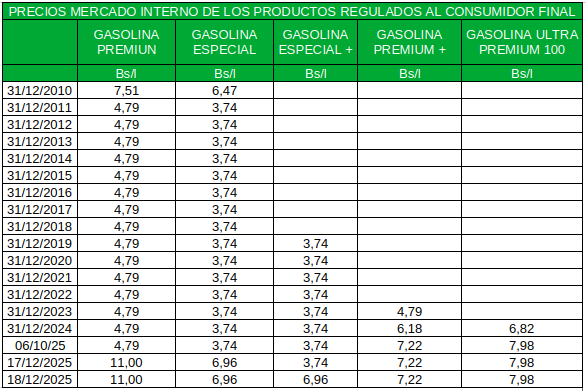
\includegraphics[width=0.9\textwidth]{Images/ANH.png}
	\vspace{0.2cm}
	
	% 3. La nota de fuente formateada según APA 7
	\begin{flushleft}
		\footnotesize \textit{Nota.} El gráfico muestra la tendencia histórica del costo del combustible. Tomado de \citep{anh_calidad_2024}.
	\end{flushleft}
\end{figure}

Asimismo, una combustión ineficiente asociada a combustibles de calidad variable puede influir en las lecturas de los sensores del vehículo, afectando la precisión de los sistemas de diagnóstico basados en OBD-II. Esto dificulta la interpretación adecuada de los parámetros del motor y limita la capacidad del usuario para evaluar el estado real de su vehículo.

En este escenario, surge una creciente preocupación sobre la eficiencia en el uso de la gasolina como fuente energética en el transporte, especialmente en vehículos que no cuentan con sistemas avanzados de monitoreo. La falta de herramientas accesibles que permitan analizar el consumo de combustible en tiempo real incrementa la incertidumbre del usuario respecto al rendimiento de su vehículo.

Por lo tanto, se plantea la necesidad de desarrollar un sistema que permita monitorear y analizar el consumo de combustible de manera precisa y en tiempo real, con el objetivo de contribuir a la optimización de la eficiencia energética del vehículo y brindar al usuario información confiable para la toma de decisiones \citep{lamby2026giro}.



\section{Justificación}

En el transporte urbano de La Paz, los vehiculos con sistemas de inyección electrónica operan sin herramientas que permitan conocer de manera precisa y continua el consumo real de gasolina durante su funcionamiento. En la práctica, la evaluación del consumo se realiza de forma empírica, sin información técnica que permita identificar ineficiencias en el uso del combustible.

La ausencia de sistemas de monitoreo del consumo dificulta el análisis del comportamiento del motor, tales tramos recorridos y modos de conducción. Esta situación limita la posibilidad de optimizar el desempeño del vehículo y detectar posibles fallas asociadas a un consumo anómalo de combustible El proyecto ayuda a tener un patrón o un control que indica si el vehículo consume mas gasolina de la que debe, considerando las condiciones en la ciudad de La Paz.

El desarrollo de un sistema permitirá generar información confiable sobre el comportamiento del motor. Esta información contribuirá a la mejora de la eficiencia operativa, al análisis técnico del consumo de combustible y al apoyo en procesos de mantenimiento y toma de decisiones técnicas.
\begin{itemize}
	\item \textbf{Justificación técnica:}
	El proyecto propone el desarrollo de un sistema de monitoreo del consumo de gasolina basado en la adquisición de parámetros del motor a través del puerto OBD-II y su procesamiento mediante un modelo físico-matemático del proceso de inyección de combustible. A diferencia de los métodos convencionales basados únicamente en mantenimiento correctivo o preventivo \citep{Reif2015}, la propuesta integra una plataforma telemétrica capaz de adquirir datos del vehículo, permitiendo el análisis casi en tiempo real del comportamiento del motor.
	
	\item \textbf{Justificación económica:}
	El acceso a información precisa y continua sobre el consumo de combustible permite a conductores y operadores de transporte optimizar el uso del vehículo, reduciendo gastos innecesarios asociados al consumo excesivo de gasolina. Asimismo, el sistema contribuye a la toma de decisiones relacionadas con el mantenimiento del motorizado y la planificación de rutas, generando un impacto económico positivo tanto para transportistas como para usuarios.
	
	\item \textbf{Justificación social:}
	El sistema propuesto aporta a la mejora de la eficiencia del transporte urbano y vehículos de uso particular, al promover un uso más responsable del combustible. Esto contribuye indirectamente a una mayor transparencia en el desempeño de los vehículos, a la concienciación sobre el consumo energético y a la mejora de la calidad del servicio de transporte en la ciudad de La Paz.
\end{itemize}

\section{Objetivos del proyecto}
\subsection{Objetivo General}
\begin{itemize}
	\item Desarrollar e implementar un sistema embebido capaz de adquirir datos en tiempo real desde el puerto de diagnóstico vehicular mediante el estándar OBD-II, con el fin de estimar el consumo instantáneo de combustible en vehículos a gasolina con inyección electrónica, generar un registro histórico de consumo y validar los resultados respecto a mediciones de referencia.
\end{itemize}

\subsection{Objetivos específicos}
\begin{itemize}
	\item Determinar los parámetros del sistema OBD-II disponibles, particularmente el flujo de aire del motor (MAF) y/o presión de aire del motor (MAP), las RPM y la velocidad del vehículo, con el fin de estimar el consumo de combustible mediante un modelo matemático basado en la relación aire-combustible.
	
	\item Desarrollar un modelo matemático para la estimación del consumo de combustible del transporte público de la ciudad de La Paz, utilizando parámetros obtenidos mediante el sistema OBD-II, basado en la relación aire--combustible del proceso de combustión.
	
	\item Adquirir y registrar datos del funcionamiento del motor mediante el sistema OBD-II, particularmente el flujo másico de aire (MAF) y/o presión de aire del motor (MAP), las revoluciones por minuto (RPM) y la velocidad del vehículo, para su posterior análisis en el modelo de estimación del consumo de combustible. Como se menciona en \citep{shaw2019fuel}, es posible estimar el consumo instantáneo de combustible utilizando datos obtenidos del vehículo mediante interfaces OBD-II.
	
	\item Diseñar un sistema embebido de adquisición de datos para la captura, el guardado y posterior procesamiento de estos, facilitando la validación del modelo matemático de consumo de combustible del transporte público de La Paz.
	
	\item Diseñar e implementar una plataforma telemétrica basada en arquitectura IoT para la adquisición de parámetros del motor a través de la interfaz OBD-II utilizando un módulo ESP32  conectado a un adaptador , permitiendo la transmisión de los datos mediante un protocolo de comunicación hacia un servidor local donde serán almacenados en una base de datos estructurada para su posterior análisis del consumo de combustible.
	
	\item Evaluar el sistema integral del transporte público de La Paz bajo condiciones reales, validando su precisión en la estimación del consumo de combustible y su contribución a la mejora de la eficiencia energética.
	
\end{itemize}

\section{Alcances y limites}
\subsection{Alcances}
El presente proyecto tiene como alcance el desarrollo de un sistema de monitoreo del 
consumo de combustible basado en la adquisición de datos a través del puerto OBD-II 
del vehículo, utilizando un microcontrolador ESP32C3 y un módulo de comunicación CAN.
El sistema tendrá los siguientes alcances:

\begin{itemize}
	\item Lectura de parámetros vehiculares en tiempo real, tales como revoluciones 
	del motor (RPM), velocidad del vehículo y otras variables disponibles mediante el 
	protocolo OBD-II, las cuales serán utilizadas para la estimación del consumo 
	de combustible.
	
	\item Procesamiento de los datos obtenidos con el fin de generar información 
	comprensible para el usuario, permitiendo evaluar el rendimiento del vehículo 
	en función de su consumo energético.
	
	\item Desarrollo de una interfaz de monitoreo accesible mediante una página web 
	generada por el propio ESP32, disponible a través de una dirección IP local, 
	que permitirá la visualización de los datos en tiempo real sin necesidad de 
	software adicional.
	
	\item Diseño, implementación y validación del sistema en condiciones reales de 
	funcionamiento, permitiendo verificar su desempeño en la estimación del consumo 
	de combustible.
\end{itemize}
\subsection{Limites}

La solución propuesta presenta ciertas limitaciones técnicas y de alcance que deben ser consideradas para una correcta interpretación de los resultados.

\begin{itemize}
	\item Una de las principales limitaciones está relacionada el tipo de combustible del vehículo.El desarrollo se enfoca exclusivamente a vehículos a gasolina con inyección electrónica, también no se enfoca a vehículos con diésel o con sistemas de combustible combinado, conocidos como vehículos \textit{bi-fuel}, los cuales pueden operar tanto con gasolina como con gas natural o GLP. Debido a que el comportamiento físico y energético de estos combustibles es diferente, el sistema propuesto se enfoca únicamente en vehículos que operan exclusivamente con gasolina, no siendo posible un control preciso del consumo en vehículos bi-fuel \citep{AFDC_BiFuelVehicles}.
	\item Asimismo, los vehículos de modelos antiguos que cuentan con sistemas de diagnóstico OBD-I presentan una limitación importante, ya que no permiten el acceso a información estandarizada del motor. Por esta razón, el sistema se encuentra limitado a vehículos que disponen de puerto OBD-II o sistemas de diagnóstico compatibles.
	\item En el contexto del transporte público en la ciudad de La Paz, la compatibilidad con sistemas de diagnóstico a bordo OBD-II se encuentra en vehiculos de fabricación relativamente reciente. En el presente trabajo se considerarán únicamente modelos que dispongan de esta tecnología, sin especificar marcas o versiones comerciales particulares.
	No obstante, el análisis experimental se limitará exclusivamente a unidades seleccionadas que cumplan con el requisito de compatibilidad OBD-II.
	\item Una de las limitaciones del presente estudio es la disponibilidad de
	vehículos para la realización de las pruebas experimentales. Al no disponer
	de acceso directo y permanente a unidades específicas como en el caso de los minibuses. Por esta razón, las pruebas experimentales podrán
	realizarse también en otros vehículos con características mecánicas
	similares que formen parte del parque automotor urbano y que
	cuenten con sistemas de inyección electrónica compatibles con la
	interfaz OBD-II.
	\item Adicionalmente, la precisión del sistema dependerá del estado mecánico del vehículo . En vehículos con alto kilometraje o desgaste significativo, los valores obtenidos pueden presentar variaciones respecto a los valores ideales.
\end{itemize}
\clearpage
	\chapter{MARCO TEÓRICO}
%--------------------------2.1-----------------
\section{Unidad de control electrónica ECU}

La \textit{Engine Control Unit} (ECU), o Unidad de Control del Motor, es un módulo electrónico encargado de gestionar el funcionamiento del motor de combustión interna, así como de otros sistemas del vehículo \citep{Bosch_EngineManagement, Heywood2018}. 

En términos simples, la ECU funciona como la “computadora central” del motor y se ve fisicamente como en la Figura \ref{fig:ecu}  recibe señales de sensores, las procesa y emite órdenes a actuadores como inyectores, válvulas de mariposa, sistemas de encendido y ventiladores para mantener el motor funcionando de manera eficiente, segura y dentro de los límites de emisiones permitidos \citep{AcademiaLab_ECU, ClubAuto_ECUfuncionamiento}.

\begin{figure}[h]
	\centering
	
	% 1. El caption automático que ya tiene configurado el estilo APA 7
	\caption{Estructura de la ECU}
	\label{fig:ecu}
	\vspace{0.3cm} % Espacio entre el título y la imagen
	
	% 2. La imagen ajustada
	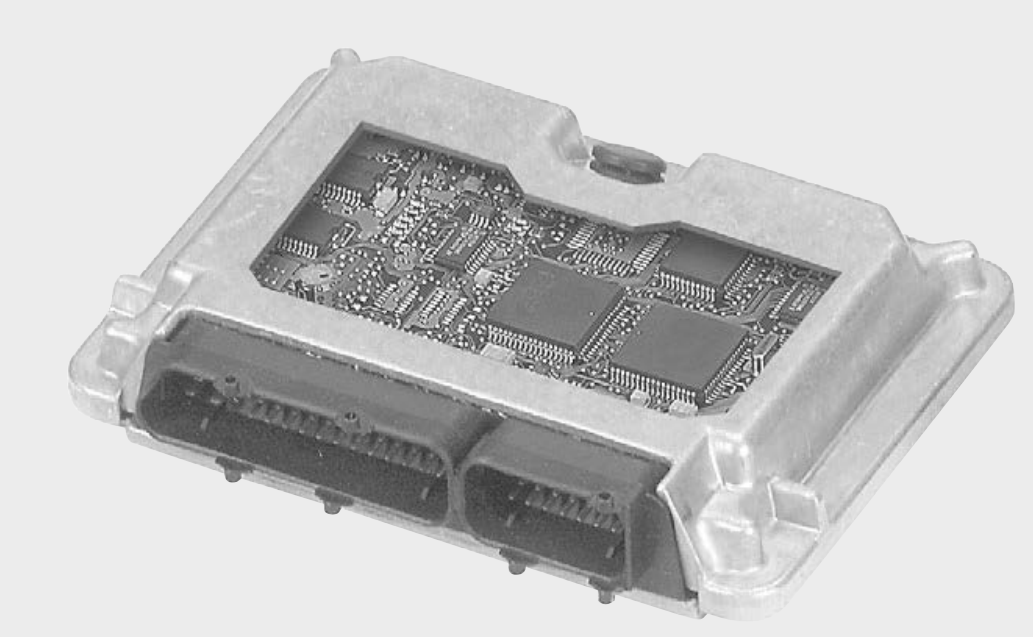
\includegraphics[width=0.75\textwidth]{Images/ECU.png}
	\vspace{0.2cm}
	
	% 3. La nota de fuente formateada según APA 7
	\begin{flushleft}
		\footnotesize \textit{Nota.} Cubierta de la carcasa abierta de una ECU. Fuente: \citep{kaiser2014electronic}.
	\end{flushleft}
\end{figure}

La ECU integra principios de electrónica, control automático y termodinámica del motor, permitiendo regular la mezcla de aire y combustible, el encendido, las emisiones y el consumo energético \citep{Heywood2018, SAE_ECU2015}. Su introducción en los vehículos modernos ha permitido optimizar el rendimiento del motor y cumplir con normas ambientales cada vez más estrictas \citep{SAE_ECU2015}.


Entre las funciones más relevantes de una ECU automotriz se pueden mencionar \citep{Bosch_EngineManagement, ClubAuto_ECUfuncionamiento, Autoavance_ECU2020}:

\begin{itemize}
  \item \textbf{Control de la inyección de combustible}: ajuste de la cantidad, el momento y la duración del chorro de combustible en cada cilindro según la carga del motor, la temperatura del refrigerante, la presión de admisión y otros parámetros.
  \item \textbf{Control del sistema de encendido}: determinación del avance del encendido (ángulo de bujía) para optimizar la combustión de la mezcla aire‑combustible.
  \item \textbf{Control de la admisión de aire}: regulación de la válvula de mariposa, el acelerador electrónico y dispositivos de recirculación de gases (EGR, turbocompresión, etc.) para el caudal de aire al motor.
  \item \textbf{Diagnóstico y monitorización del motor}: detección de anomalías, activación de luces de advertencia en el panel (MIL) y almacenamiento de códigos de falla mediante el sistema OBD‑II.
  \item \textbf{Gestión de otros sistemas}: en vehículos avanzados, la ECU o sus módulos asociados (ECM, PCM, VCM) pueden intervenir en el control de la transmisión automática, el sistema de carga y el aire acondicionado.
\end{itemize}

\subsection{Tipos de modulo de control}
\begin{itemize}
    \item \textbf{ECM} (engine control module), modulo de control del motor.Controla y almacena únicamente los códigos de diagnóstico de fallas (DTCs) de los componentes del motor.
    \item \textbf{PCM} (train power control module), modulo de control del tren de potencia. Controla y almacena datos del motor y la transmisión.
    \item \textbf{VCM} (vehicle control module), modulo de control del vehículo. Controla y almacena datos del motor, la transmisión y otros sistemas del vehículo como sistemas de frenos ABS.\citep{poudel2018design}
\end{itemize}

\subsection{Estructura interna de la ECU} % (microprocesador, memoria, entradas/salidas)
La estructura interna de una ECU se basa en un sistema de hardware y software integrado, donde el núcleo principal es un microcontrolador (CPU) encargado de procesar en tiempo real las señales provenientes de sensores y emitir órdenes a los actuadores del motor \citep{Bosch_EngineManagement, Heywood2018}. Alrededor de este microcontrolador se disponen memorias de tipo flash y ROM, que almacenan el firmware y los mapas de encendido e inyección, así como memoria RAM utilizada para cálculos y variables de estado durante el funcionamiento \citep{Wikipedia_ECU, ClubAuto_ECUfuncionamiento}. 

Además, la ECU integra módulos de acondicionamiento de señales de entrada (filtros, amplificadores y convertidores analógico‑digital) y etapas de potencia de salida (drivers de transistores o MOSFET) para activar correctamente actuadores como inyectores de combustible, válvulas solenoides y ventiladores de refrigeración \citep{Autoavance_ECU2020}.
Y se divide en los siguientes sistemas.

\begin{itemize}
    \item \textbf{Periferia} Consta de elementos pasivos resistencias, capacitores. 
    \item \textbf{Circuitos de filtrado} Filtros pasa bajos para contrarrestar ruido y mejorar la señal. 
    \item \textbf{Fuente} Elementos pasivos y semiconductores resistencias, capacitores, diodos y reguladores de tensión. 
    \item \textbf{Procesamiento de datos} Usa 2 sistemas clave, la memoria la que almacena todos los datos, y el procesador que lee todos los datos. 
    \item \textbf{Driver} Maneja todos los actuadores: transistores, drivers para motores de paso. 
    \item \textbf{Multiplexor} Comparte datos con otras ECUS. 
\end{itemize}

Todos los sistemas mencionados se muestran en conjunto en la Figura \ref{fig:a_ecu}

\begin{figure}[h]
	\centering
	
	% 1. El caption automático con estilo APA 7 (Título arriba)
	\caption{Arquitectura interna de la ECU}
	\label{fig:a_ecu}
	\vspace{0.3cm}
	
	% 2. La imagen
	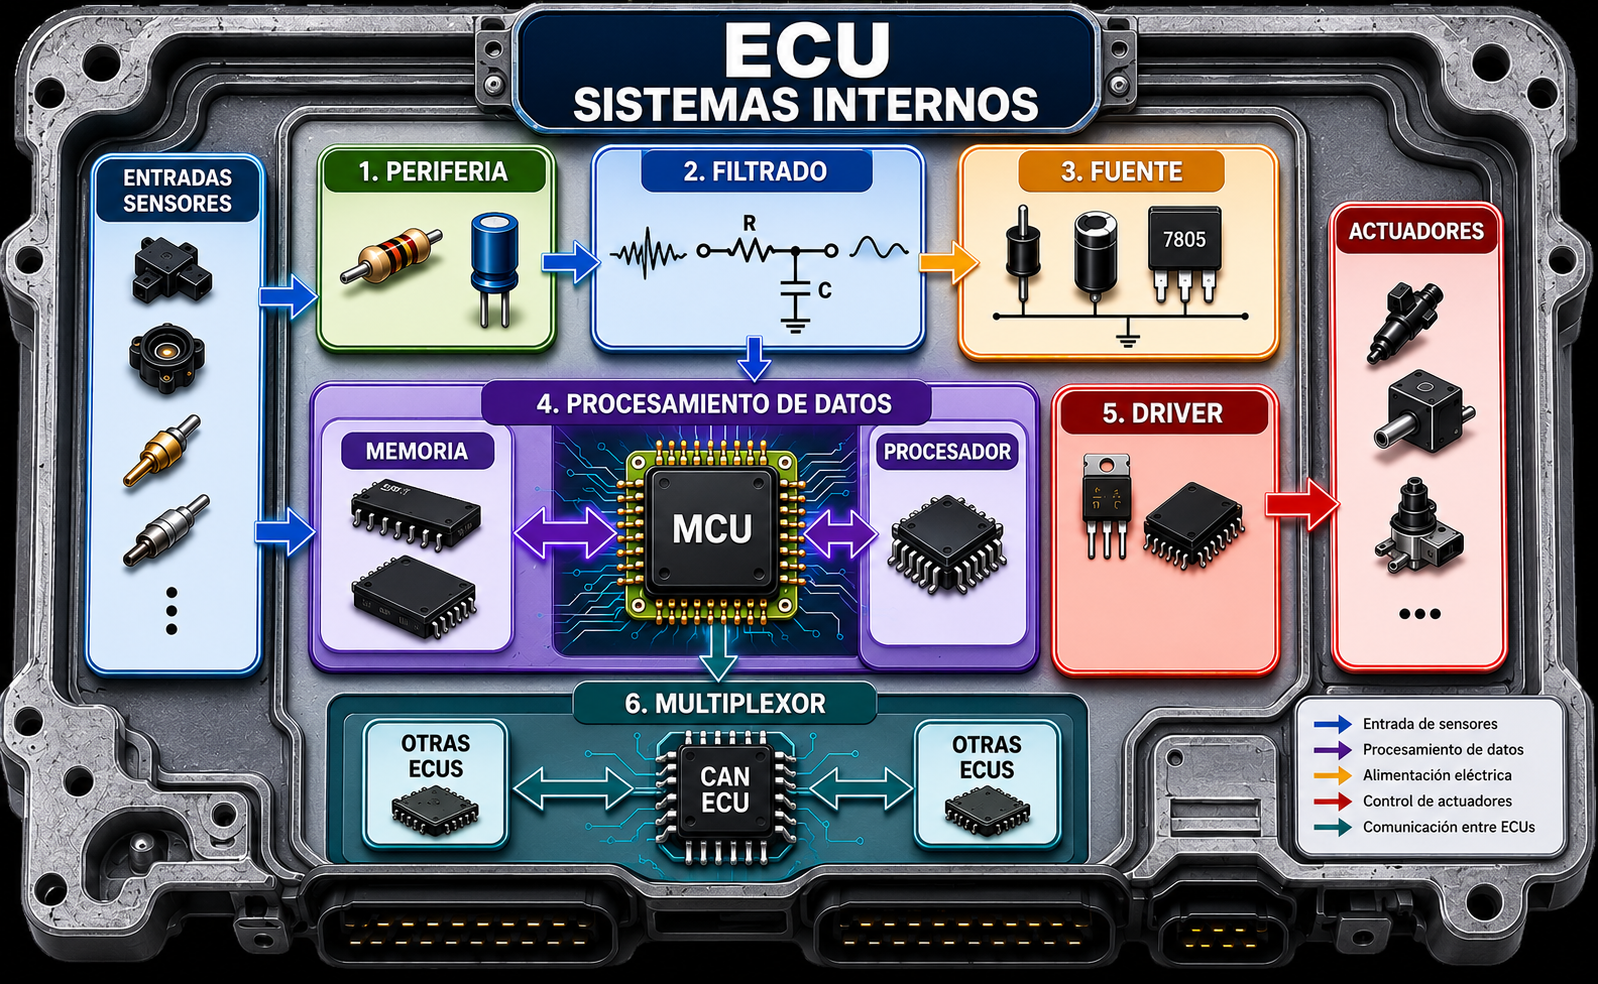
\includegraphics[width=0.9\textwidth]{Images/ESTRUCTURA.png}
	\vspace{0.2cm}
	
	% 3. La nota de fuente formateada según APA 7
	\begin{flushleft}
		\footnotesize \textit{Nota.} Arquitectura interna y conjunto de sistemas dentro de la unidad de control. Elaboración propia basada en \citep{poudel2018design} y generada con apoyo de inteligencia artificial (Gemini).
	\end{flushleft}
\end{figure}

\subsubsection{Procesamiento de señales} % (cómo la ECU interpreta datos)
Para que el microprocesador pueda interpretar las señales de los sensores (señales de entrada), estas deben ser convertidas en el módulo de control electrónico de analógicas a digitales. Estas señales luego son acompañadas con los parámetros lógicos grabados en la memoria y luego será elaborada la orden o señales de salida a los actuadores. 

Se muestra un diagrama general del procesamiento de la ECU en la Figura \ref{fig:dia_pro}.

\begin{figure}[h]
	\centering
	
	% 1. El caption automático estilo APA 7 (Título arriba)
	\caption{Diagrama de procesamiento de la ECU}
	\label{fig:dia_pro}
	\vspace{0.3cm}
	
	% 2. La imagen
	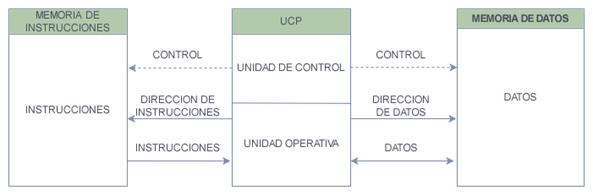
\includegraphics[width=0.8\textwidth]{Images/DIAGRAM.png}
	\vspace{0.2cm}
	
	% 3. La nota de la figura según APA 7
	\begin{flushleft}
		\footnotesize \textit{Nota.} Secuencia lógica de las etapas de entrada, procesamiento y salida de datos en la unidad de control. Elaboración propia.
	\end{flushleft}
\end{figure}

\subsubsection{Parámetros de control del motor} % (mezcla aire-combustible, avance de encendido)
Es necesario diferenciar bien cada una de las fases que esta debe realizar para enviar señales a los diferentes actuadores del vehículo.\\
Para ello se divide el estudio en cuatro bloques de funcionamiento. 
\begin{itemize}
    \item \textbf{Bloque de entrada} Se denomina bloque de entrada a todos los circuitos que se encuentran como receptores de las diferentes señales que van a ingresar a la ECU y antes de que lleguen al microprocesador. Encontramos en este sentido, filtros, amplificadores, conformadores de impulsos, conversores análogos a digital. 
    \begin{itemize}
        \item Regulador de tensión.- El regulador de tensión (5V) es utilizado como señal de entrada para casitodos los sensores de inyección y para la operación interna de memorias y el microprocesador del módulo de control electrónico.
        La tensión regulada es mantenida a pesar de las variaciones de tensión de la batería en 5V ± 15%
        \item Filtrado de señales.-  Los filtros digitales tienen como entrada una señal analógica o digital y en su salida tienen otra señal analógica o digital, pudiendo haber cambiado en amplitud, frecuencia o fase dependiendo de las características del filtro digital. 
        \item Conformadores de impulso.- Actúa para recibir los impulsos de tensión de los órganos de información del encendido. Estos impulsos son modificados en magnitud y en forma, para dejarlos en condiciones que puedan ser procesados por el micro-ordenador. 
        \item Convertidor Análogo – Digital.- La señal que recibe el módulo de control electrónico desde los sensores, no puede ser interpretada por el microprocesador, por lo tanto las señales de los sensores que son análogas, deben ser convertidas a digitales.\\
        Para esta conversión se utilizan transistores de saturación o corte, que se comportan exactamente igual a un relé activado-desactivado. 
    \end{itemize}
    \item \textbf{Bloque de procesamiento} Son todos los circuitos que desarrolla las funciones programadas y que están constituidos circuitalmente por el procesador, memorias y todo circuito que se vea involucrado en la ejecución del software. 
    \begin{itemize}
        \item \textbf{Memorias.-} Es esta se realizan los cálculos matemáticos de acuerdo a las señales de entrada; la memoria se borra cuando se apaga el motor. 
        \begin{itemize}
            \item \textbf{Memoria RAM (Random Access Memory):} El microprocesador utiliza la memoria RAM para saber el estado general y las condiciones del motor y en función a esto hacer funcionar los actuadores. 
            \item \textbf{Memoria KAM (Keep Alive Memory):} La memoria KAM vive con la memoria RAM y su función es de guardar los datos que no se pueden perder al cerrar el contacto, como por ejemplo códigos de fallas aleatorias de sensores.
            
            A diferencia de la memoria RAM, la KAM no se borra al cerrar el contacto, pero si se borra al desconectar la batería.
            
            Cuando en la memoria KAM se almacena un defecto, este permanecerá instalado aun después de ser corregido, debiendo desconectar la batería para que se borre o en algunos casos, se debe proceder al borrado con un scanner. 
            \item \textbf{Memoria EPROM (Erasable Programmable Read Only Memory):} En la memoria EPROM (programable) o PROM (programada) es donde el microprocesador consulta todas las calibraciones del vehículo, tales como el peso del mismo y la compresión del motor. Al cerrar el contacto o desconectar la batería, esta memoria no se borra. 
            \item \textbf{Memoria ROM (Read Only Memory):} Esta memoria mantiene grabados los programas con todos los datos, curvas características y valores teóricos con los que ha de funcionar el sistema.
            
            Esta memoria es utilizada por el microprocesador para comparar los parámetro de cada sensor en cada situación y en los casos en que el microprocesador detecte alguna anomalía en alguna señal, la reemplazará por un valor de la memoria ROM.
            
            La memoria ROM es una memoria de consulta y al igual que la memoria EPROM no se borra ni al cerrar el contacto, ni al desconectar la batería.
        \end{itemize}
        \item \textbf{Microprocesador:} Es el componente físico principal dentro de la unidad de control, encargado de ejecutar las instrucciones de software para optimizar el funcionamiento del motor. Este elemento realiza los cálculos matemáticos, la toma de decisiones y ejecuta las estrategias de emergencia.
        Contiene en su interior tres dispositivos fundamentales:
        \begin{itemize}
            \item \textbf{Unidad lógica de calculo (ALU):}Realiza las operaciones aritméticas y las operaciones lógicas.
            \item \textbf{Acumulador:} Es una memoria intermedia que permite al CPU guardar datos mientras trabaja con otros que están directamente relacionados con el proceso en curso.
            \item \textbf{Unidad de control:} Es el elemento activo que solicita los datos, controla las entradas, las salidas y el desarrollo de las operaciones.
        \end{itemize}
        
    \end{itemize}

    \item \textbf{Bloque de salida} Así como las señales son tratadas al ingresar, existen circuitos que se encuentran entre las salidas del microprocesador y los diferentes elementos que van a ser actuados como por ejemplo: bobinas de encendido, inyectores, relés, etc. \\
    Tenemos los siguientes componentes importantes en este bloque:
    \begin{itemize}
        \item Convertidor digital - análogo.- Así como las señales de los sensores deben ser transformadas en digitales, para que puedan ser interpretadas por el microprocesador y de esta forma “saber lo que está pasando La señal digital debe convertirse en analógica para controlar los actuadores(señales analógicas).
        
        De esta forma es que todas las señales micro procesadas son convertidas de digitales en análogas para controlar a los actuadores. El convertidor digital recibe un número de 8 BITS y la trasforma en una tensión continua de un valor proporcional al número digital.
        \item Drivers (Controlador de dispositivo).- El drivers están básicamente diseñado para controlar los actuadores, como por ejemplo los inyectores, bobinas, relés, entre otros, estos circuitos deben cumplir con requisitos de manejo de potencia puesto que la corriente que se maneja en muchos de ellos alcanza los 5A y los voltajes operados pueden llegar a picos de hasta 400V.
        \begin{itemize}
            \item Transistores
            \item Circuitos integrados de control
        \end{itemize}
        \item Circuitos de potencia con transistores.- Se encargan de dar los pulsos de activación a las bobinas de encendido, inyectores, relés, etc. para de esta manera poner en funcionamiento a cada uno de los actuadores. 
        
   \end{itemize}
    \item \textbf{Bloque de soporte}  Se denomina así al conjunto de componentes que tienen como función alimentar a los circuitos internos mencionados anteriormente. Lo constituye la fuente de alimentación de la ECU.
    \begin{itemize}
        \item Regulador de voltaje.-
        \item Fuente de alimentación de la ECU.- Los ECM disponen de una fuente de poder interna que proporciona distintos tipos de voltajes para energizar componentes como sensores y Actuadores. Estos voltajes pueden tener una variación.\\Conformados por:
        \begin{itemize}
            \item Diodos rectificadores y zener.
            \item Condensadores.
            \item Reguladores de Tensión.
            \item Resistencias.
        \end{itemize}
    \end{itemize}
    Datos importante de la parte de bloque de soporte:
    \begin{itemize}
        \item + 5 volt. + - 0.5 V voltaje de suministro para sensores análogos.
        \item + 8 volt. + - 0.5 V voltaje de suministro para sensores digitales o PWM.
        \item + 12,5 volt. + - 1V voltaje de suministro para sensores de frecuencia electrónicos.
        \item + 105 volt. + - 0.5 voltaje de suministro para solenoides para inyección de combustible.
    \end{itemize}
    Para el negativo, existen tres posibilidades de masas en una ECU, estas son: 
    \begin{itemize}
        \item \textbf{Masa digital:} Usada por la ECU para el sistema de procesamiento de datos, Procesador y Memoria.
        \item \textbf{Masa análoga:} Usada por la ECU para circuitos análogos, por ejemplo conversores análogos a digital.
        \item \textbf{Masa de potencia:} Usada por la ECU para circuitos de fuente y control de actuadores principalmente ej. , regulador de tensión y principalmente transistores.
        \item \textbf{Masa de blindaje:} La Ecu posee un circuito de blindaje, el cual es capaz de transportar las señales dentro de la ECU sin la presencia de ruido electromagnético.
    \end{itemize}
\end{itemize}

Se presenta un resumen en la Figura \ref{fig:esquema_ecu}

\begin{figure}[h]
	\centering
	
	% 1. El caption automático estilo APA 7 (Título arriba)
	\caption{Esquema de la unidad de control electrónica ECU}
	\label{fig:esquema_ecu}
	\vspace{0.3cm}
	
	% 2. La imagen ajustada al ancho del texto para evitar Overfull \hbox
	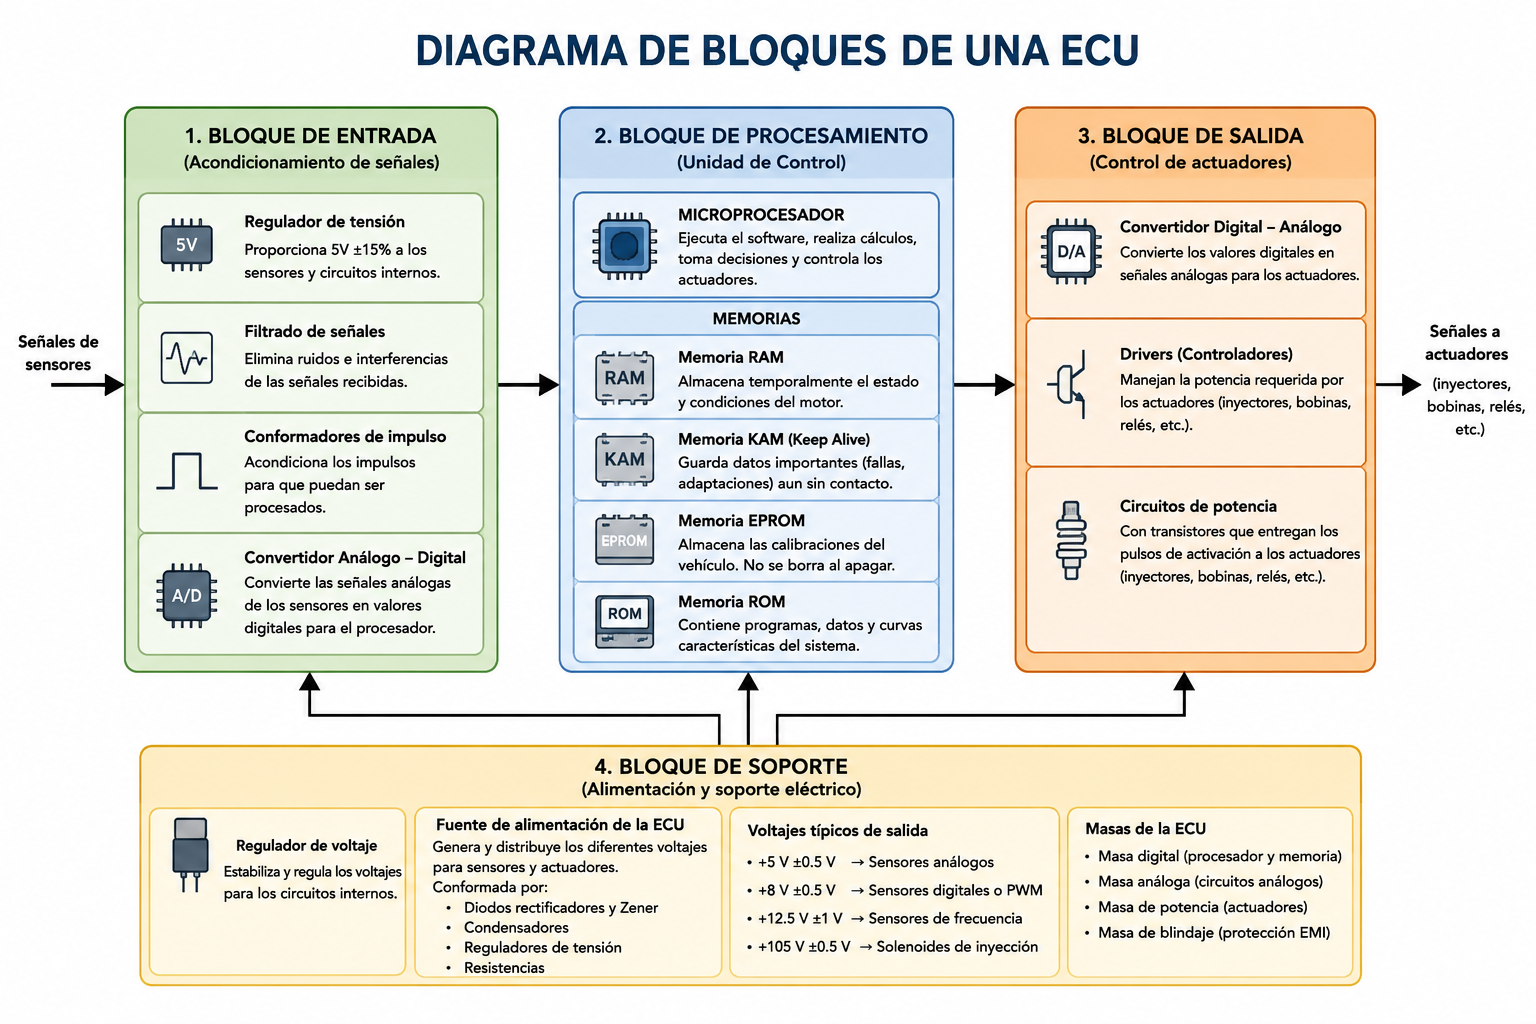
\includegraphics[width=1.0\textwidth]{Images/ChatGPT.png}
	\vspace{0.2cm}
	
	% 3. La nota de la figura según APA 7
	\begin{flushleft}
		\footnotesize \textit{Nota.} Diagrama esquemático integral de los bloques funcionales de la unidad de control. Elaboración propia, generada con apoyo de inteligencia artificial (Gemini).
	\end{flushleft}
\end{figure}

\subsection{Importancia de la ECU en el consumo de combustible}
La ECU desempeña un papel fundamental en la optimización del consumo de combustible, actúando como el elemento central que regula la mezcla aire‑combustible, el encendido, la admisión de aire y la gestión general del motor \citep{Bosch_EngineManagement, Heywood2018}. Mediante el uso continuo de sensores de presión de admisión, temperatura, posición del acelerador, velocidad y carga, la ECU ajusta en tiempo real la cantidad de combustible inyectado, el avance del encendido y el flujo de aire, favoreciendo siempre una combustión lo más completa y eficiente posible \citep{SAE_ECU2015, ClubAuto_ECUfuncionamiento}.

Esta regulación permanente permite que el motor funcione cerca de su punto óptimo de eficiencia en una amplia gama de condiciones de conducción, lo que se traduce en una reducción del consumo específico de combustible y en menores emisiones contaminantes \citep{AcademiaLab_ECU, CentralitaBSI_EficienciaCombustible}. 

Además, en vehículos con transmisión automática, la ECU colabora con otros módulos de control (por ejemplo, ECU de transmisión) para seleccionar el momento más adecuado para cambiar de marcha, lo que contribuye a mantener el motor en rangos de revoluciones donde el consumo de combustible es más bajo \citep{SAE_ECU2015, PedalCommander_ECUtuning}.

Por lo tanto la cantidad de combustible a inyectar es determinado teniendo en cuenta también la cartografía de inyección que esta memorizada en la unidad de control y que intenta en todo momento evitar la emisión de contaminantes (humo negro) ver Figura \ref{fig:carto}. Si el volumen de aire aspirado es demasiado bajo la cantidad de combustible inyectado es limitado a un valor que no provoque humos negros.

\begin{figure}[h]
	\centering
	
	% 1. El caption automático estilo APA 7 (Título arriba)
	\caption{Cartografía de inyección}
	\label{fig:carto}
	\vspace{0.3cm}
	
	% 2. La imagen ajustada para una mejor visualización de los datos
	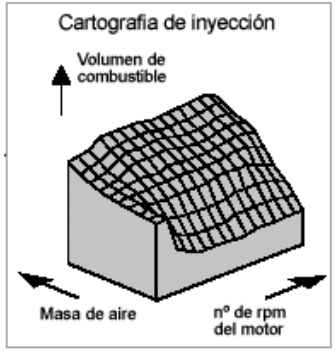
\includegraphics[width=0.5\textwidth]{Images/Conbu.png}
	\vspace{0.2cm}
	
	% 3. La nota de la figura según APA 7
	\begin{flushleft}
		\footnotesize \textit{Nota.} Mapa tridimensional de calibración que relaciona la carga del motor y las revoluciones por minuto para determinar el tiempo de inyección. Tomado de \citep{poudel2018design}.
	\end{flushleft}
\end{figure}

La unidad de control tiene memorizado un mapa de comienzo de la inyección.Este mapa toma como referencia principal el nº de rpm del motor y la cantidad de combustible inyectado ver Figura \ref{fig:rela} Como parámetro corrector se utiliza la temperatura del motor que actúa también sobre el comienzo de la inyección.

\begin{figure}[h]
	\centering
	
	% 1. El caption automático estilo APA 7 (Título conciso arriba)
	\caption{Relación de inyección entre el sensor MAP y las RPM}
	\label{fig:rela}
	\vspace{0.3cm}
	
	% 2. La imagen con su escala original
	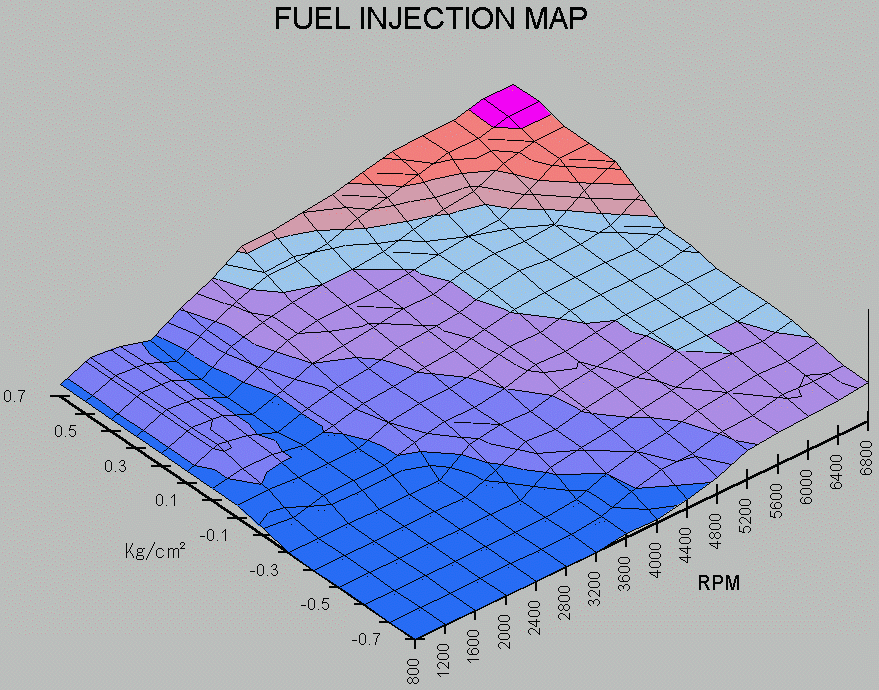
\includegraphics[width=0.63\textwidth]{Images/mAP2.png}
	\vspace{0.2cm}
	
	% 3. La nota de la figura según APA 7 (Con los detalles específicos)
	\begin{flushleft}
		\footnotesize \textit{Nota.} Comportamiento de la dosificación de combustible en un motor de cuatro tiempos operando a nivel del mar en función de la presión absoluta del colector y el régimen de giro. Tomado de \citep{ForoClubJapo_ECU}.
	\end{flushleft}
\end{figure}

En resumen, la ECU no solo mejora el rendimiento y la respuesta del motor, sino que es un componente clave para lograr una \textbf{operación económica y sostenible} del vehículo, incrementando la eficiencia del combustible sin comprometer significativamente la potencia entregada \citep{Bosch_EngineManagement, SERNAUTO_ECUeficiencia}.

%-------------------------2.2-----------------
\section{Protocolos de comunicación en vehículos}

En los vehículos modernos, la comunicación entre unidades de control electrónico (ECU) se realiza a través de diversos buses de datos en serie, que permiten integrar sistemas de motor, transmisión, chasis, seguridad y entretenimiento en una red coherente \citep{Navixy_AutomotiveBuses, MSG_CommunicationBuses}. Entre los protocolos más utilizados se encuentran CAN, LIN, FlexRay y MOST, cada uno con características distintas de velocidad, ancho de banda, costo y aplicación específica \citep{ProtocolosComunicacionAutomotriz}.

\subsection{CAN}

El protocolo \textit{Controller Area Network} (CAN) es el estándar más extendido en la comunicación interna de vehículos, utilizado para conectar unidades de control del motor (ECM), de transmisión (TCM) y sistemas de frenado (ABS), entre otros \citep{Navixy_AutomotiveBuses}. CAN opera sobre un bus de dos hilos (CAN high y CAN low) y permite la transmisión de mensajes priorizados, lo que garantiza que los datos de seguridad y dinámica del vehículo tengan mayor prioridad que los de confort o información \citep{ProtocolosComunicacionAutomotriz}. Su velocidad típica varía desde 125 kbit/s hasta 1 Mbit/s, convirtiéndolo en una solución robusta, económica y tolerante a fallos \citep{MSG_CommunicationBuses}.

\subsection{LIN}

El bus \textit{Local Interconnect Network} (LIN) es un protocolo de baja velocidad diseñado principalmente para aplicaciones de confort y comodidades, como ventanas eléctricas, espejos, luces interiores y sensores de climatización \citep{ProtocolosComunicacionAutomotriz}. Comparado con CAN, LIN es más simple y barato, ya que trabaja con un solo maestro y varios esclavos en topología maestro‑esclavo \citep{MSG_CommunicationBuses}. Aunque su velocidad máxima suele estar alrededor de 20 kbit/s, LIN es ideal para tareas poco críticas donde la prioridad es reducir costos de cableado y electrónica \citep{ProtocolosComunicacionAutomotriz}.

\subsection{FlexRay}

El protocolo FlexRay es un bus de alta velocidad y baja latencia orientado a aplicaciones críticas, como sistemas de conducción avanzada, control de chasis y vehículos autónomos \citep{Navixy_AutomotiveBuses, Autoavance_FlexRay}. FlexRay ofrece tiempos de respuesta deterministas y soporta tasas de transferencia de hasta 10 Mbit/s, lo que permite manejar grandes volúmenes de datos en tiempo real \citep{MSG_CommunicationBuses}. Además, su topología dual‑canal permite redundancia y alta disponibilidad, características clave para funciones de seguridad que no admiten interrupciones \citep{Autoavance_FlexRay}.

\subsection{MOST}

El bus MOST (\textit{Media Oriented Systems Transport}) está dedicado a la transmisión de datos multimedia, como audio, video y señales de info‑entretenimiento, dentro del vehículo \citep{Navixy_AutomotiveBuses}. MOST utiliza un anillo óptico o eléctrico y soporta velocidades de 25, 50 o 150 Mbit/s, permitiendo integrar pantallas, sistemas de navegación, reproductores de audio y dispositivos de comunicación sin afectar las redes de control principal \citep{ProtocolosComunicacionAutomotriz}. Su diseño está orientado a mantener alta calidad de señal y bajo retardo en el transporte de flujos multimedios, separando esta red de la red de control motor‑tracción construida sobre CAN o FlexRay \citep{ProtocolosComunicacionAutomotriz}.

El resumen de lo abordado se presenta en la Tabla \ref{table:caract}


\begin{table}[htbp]
	\centering
	% Título separado bajo norma estricta APA 7
	\captionsetup{labelformat=simple, labelsep=newline, textfont=it, labelfont=bf}
	\caption{Comparación de los protocolos de comunicación en vehículos}
	\label{table:caract}
	\vspace{0.3cm}
	
	\begin{tabularx}{\linewidth}{p{2.4cm} X X X X}
		\toprule 
		\rowcolor[rgb]{0.851, 0.851, 0.851}
		\textbf{Ítem} & \textbf{CAN} & \textbf{LIN} & \textbf{FlexRay} & \textbf{MOST} \\
		\midrule 
		Velocidad típica & 125 kbit/s a 1 Mbit/s & Hasta 20 kbit/s & Hasta 10 Mbit/s & 25, 50 o 150 Mbit/s \\
		Aplicación & Control de motor, transmisión, ABS & Comodidades (ventanas, espejos, luces) & Sistemas de seguridad y conducción avanzada & Multimedia (audio, video, infoentretenimiento) \\
		Topología & Bus multidifusión robusto & Maestro-esclavo, sencillo & Dual-canal redundante & Anillo óptico o eléctrico \\
		Prioridad & Alta, con priorización de datos críticos & Baja, tareas no críticas & Alta, determinista & Media, orientado a multimedia \\
		Costo & Moderado & Bajo & Alto & Alto \\
		Latencia & Media & Alta & Muy baja & Media \\
		\bottomrule 
	\end{tabularx}
	\vspace{0.2cm}
	
	\begin{flushleft}
		\footnotesize \textit{Nota.} Elaboración propia.
	\end{flushleft}
\end{table}


%-------------------------2.3----------------
\section{Sistema OBD-II}
\subsection{Evolución del diagnóstico a bordo}

El diagnóstico a bordo, conocido como OBD (\textit{On-Board Diagnostics}), evolucionó desde sistemas muy básicos de monitoreo hasta convertirse en una herramienta estandarizada y esencial para la detección de fallas en vehículos modernos. Sus primeras aplicaciones aparecieron en la década de 1960 con sistemas de diagnóstico analógicos, y posteriormente, en las décadas de 1970 y 1980, los fabricantes comenzaron a incorporar funciones electrónicas capaces de almacenar información sobre el funcionamiento del motor y registrar anomalías \citep{Geotab_OBDII}. La estandarización del sistema avanzó a finales de los años ochenta, cuando se impulsó el uso de conectores y protocolos comunes, lo que permitió que los escáneres pudieran leer códigos de falla de manera uniforme en distintos vehículos. 

Con la llegada del OBD-II en la década de 1990, el diagnóstico se volvió más completo, permitiendo supervisar sistemas relacionados con emisiones, rendimiento del motor y sensores críticos, facilitando así el mantenimiento preventivo y la reducción de contaminantes \citep{Geotab_OBDII, OBDII_HistoriaFuncion}.

Para llevar a cabo dichos diagnósticos, se emplean convencionalmente escáneres automotrices capaces de recopilar la información mencionada a través del puerto OBD-II; este instrumento se muestra en la Figura \ref{fig:escaner}.

\begin{figure}[h]
	\centering
	
	% 1. El caption automático estilo APA 7 (Título conciso arriba)
	\caption{Escáner automotriz}
	\label{fig:escaner}
	\vspace{0.3cm}
	
	% 2. La imagen con su escala original
	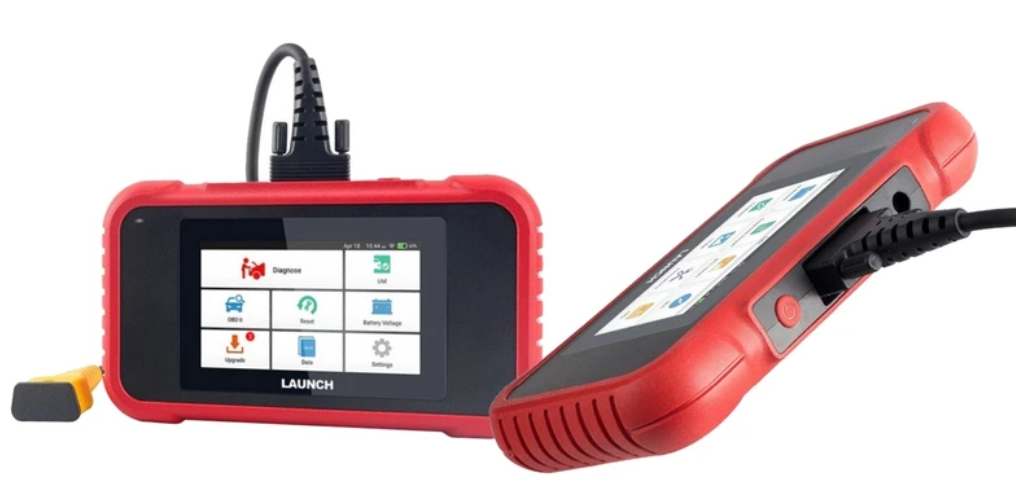
\includegraphics[width=0.63\textwidth]{Images/escaner.png}
	\vspace{0.2cm}
	
	% 3. La nota de la figura según APA 7
	\begin{flushleft}
		\footnotesize \textit{Nota.} Herramienta de diagnóstico electrónico utilizada para la lectura de códigos de falla y monitoreo de parámetros a través de la interfaz del puerto OBD-II. Tomado de \citep{OBDTester_OBD2Connector}.
	\end{flushleft}
\end{figure}

\subsection{Estructura del sistema OBD-II}% (ECU, conector, protocolos)

El sistema OBD-II está constituido por la unidad de control electrónico o ECU, el arnés de cableado, el conector de diagnóstico DLC y el protocolo de comunicación utilizado por el vehículo, que puede ser CAN, K-Line, PWM, VPW, entre otros \citep{Autoavance_OBD2, Autosoporte_OBDII, Flexihub_OBD2}. La ECU recibe señales de sensores distribuidos en el motor y, a partir del procesamiento interno, genera datos de funcionamiento, estados de actuadores y códigos de falla que pueden ser consultados a través del puerto OBD-II mediante una herramienta de diagnóstico \citep{Autoavance_OBD2, UMSA_OBDII}.

La información no sale de la ECU de forma directa hacia el escáner, sino que primero es organizada por la unidad de control en mensajes estructurados según el protocolo de comunicación del vehículo. En sistemas basados en CAN, por ejemplo, la ECU transmite y recibe tramas de datos por las líneas CAN High y CAN Low, que llegan al conector OBD-II a través del arnés eléctrico del vehículo \citep{Flexihub_OBD2, EquipoAutomotrizJAVAZ_OBD2}. En otros sistemas, la comunicación puede realizarse por una línea de datos única, como la K-Line, o por otros protocolos definidos por el fabricante \citep{Flexihub_OBD2, Autosoporte_OBDII}.

Entre la ECU y el puerto de diagnóstico intervienen principalmente el microcontrolador interno de la ECU, los circuitos de acondicionamiento de señal y los transceptores de comunicación, que adaptan los niveles eléctricos del microprocesador al bus del vehículo \citep{Autoavance_OBD2, UMSA_OBDII}. Estos transceptores permiten que la información generada dentro de la ECU sea enviada correctamente hacia el DLC sin pérdida de integridad, mientras que el escáner OBD-II actúa como elemento externo que solicita los datos y los interpreta para mostrar parámetros en tiempo real, códigos de avería y estados de sensores o actuadores \citep{Autoavance_OBD2, Autosoporte_OBDII} ver Figura \ref{fig:ecu_obd2}. De esta manera, el sistema OBD-II funciona como una interfaz estandarizada entre la electrónica interna del vehículo y el equipo de diagnóstico.

\begin{figure}[h]
	\centering
	
	% 1. El caption automático estilo APA 7 (Título arriba)
	\caption{Esquema general del flujo de información en el sistema OBD-II}
	\label{fig:ecu_obd2}
	\vspace{0.3cm}
	
	% 2. La imagen ajustada exactamente al ancho del texto
	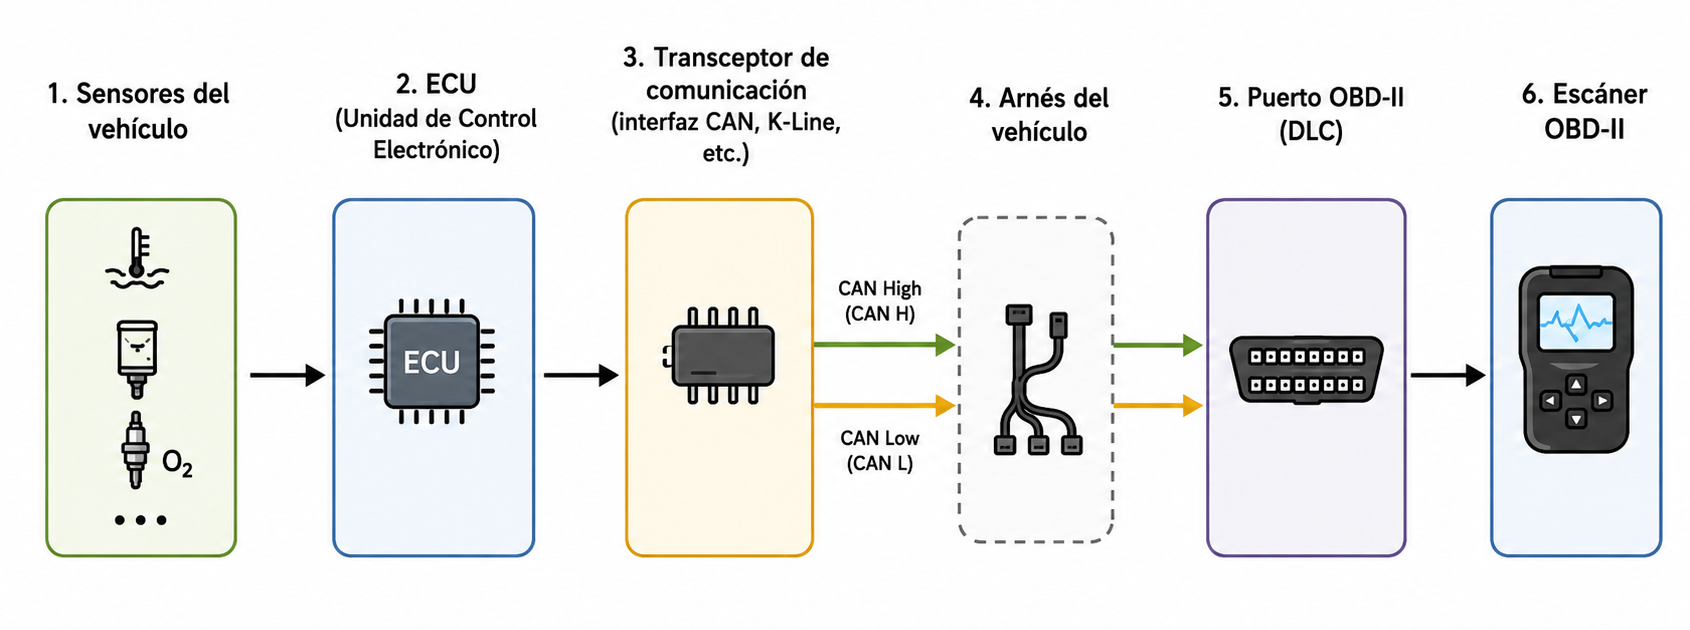
\includegraphics[width=1.0\textwidth]{Images/esquema_obd2.png}
	\vspace{0.2cm}
	
	% 3. La nota de la figura abajo alineada a la izquierda según APA 7
	\begin{flushleft}
		\footnotesize \textit{Nota.} Diagrama de bloques que describe la transmisión de datos desde la ECU y sus sensores periféricos hacia la interfaz de diagnóstico a través del bus de datos. Elaboración propia.
	\end{flushleft}
\end{figure}

\subsection{Conector OBD-II y asignación de pines}
El puerto OBD-II es una interfaz de comunicación  de 16 pines. Este puerto permite conectar dispositivos de diagnóstico, escáneres automotrices o sistemas de adquisición de datos para obtener información de las Unidades de Control Electrónico (ECU) del vehículo.  En la Figura \ref{fig:pinobd} se presenta  los pines de conexión de este puerto.

\begin{figure}[h]
	\centering
	
	% 1. El caption automático estilo APA 7 (Título conciso arriba)
	\caption{Distribución de pines del conector OBD-II}
	\label{fig:pinobd}
	\vspace{0.3cm}
	
	% 2. La imagen con su escala original
	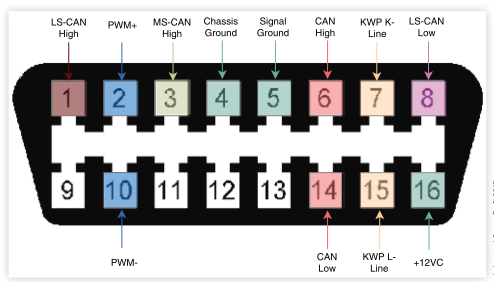
\includegraphics[width=0.5\textwidth]{Images/SEC_OBDII.png}
	\vspace{0.2cm}
	
	% 3. La nota de la figura según APA 7 (Con la descripción técnica)
	\begin{flushleft}
		\footnotesize \textit{Nota.} Configuración y asignación de los 16 pines del conector estandarizado J1962 para el diagnóstico a bordo. Tomado de \citep{OBDTester_OBD2Connector}.
	\end{flushleft}
\end{figure}

El conector OBD-II posee 16 pines, cada uno con funciones específicas dependiendo del protocolo de comunicación utilizado el detalle de cada uno de estos pines:

\begin{enumerate}
    \item LS-CAN High función específica del fabricante.
    \item Bus SAE J1850.
    \item MS-CAN High/función específica del fabricante.
    \item Tierra (chasis).
    \item Tierra de señal.
    \item CAN High (CAN alto).
    \item Línea K (ISO 9141 / ISO 14230).
    \item LS-CAN Low/función específica del fabricante.
    \item Función específica del fabricante.
    \item Bus SAE J1850/PWM.
    \item Función específica del fabricante.
    \item Función específica del fabricante.
    \item Función específica del fabricante.
    \item CAN Low.
    \item Línea L.
    \item Alimentación +12 V batería.
\end{enumerate}


En  la mayoría de los vehículos modernos, los pines 6 (CAN High) y 14 (CAN Low) son utilizados por el protocolo Controller Area Network (CAN) para la transmisión de datos entre las ECU. El puerto OBD-II puede utilizar diferentes protocolos de comunicación dependiendo del fabricante y del año del vehículo. Entre los más comunes se encuentran:
\begin{itemize}
    \item SAE J1850 PWM.
    \item SAE J1850 VPW.
    \item ISO 9141-2.
    \item ISO 14230 (KWP2000).
    \item ISO 15765-4 (CAN).
\end{itemize}

Este puerto permite solicitar información especifica mediante parámetros de identificación (Parameter ID - PIDs), los mas comunes son: 
\begin{itemize}
    \item Velocidad del vehículo.
    \item Revoluciones del motor.
    \item Temperatura del refrigerante.
    \item Posición del acelerador.
    \item Códigos de falla (DTC).
\end{itemize}
Algunas marcas permiten la visualizar una mayor cantidad de parámetros que otras, dependiendo de la cantidad de módulos con los que cuente el vehículo.
\subsection{Protocolos de comunicación}% (ISO 15765 CAN, ISO 9141, etc.)

En el sistema OBD-II existen varios protocolos de comunicación estandarizados que permiten el intercambio de información entre la ECU y el equipo de diagnóstico. En total, se consideran cinco protocolos principales de comunicación OBD-II, aunque en la práctica algunos de ellos ya han sido sustituidos por tecnologías más modernas \citep{Autoavance_OBD2, Autosoporte_OBDII, Flexihub_OBD2}.

\begin{itemize}
    \item \textbf{ISO 15765-4 CAN:} es el protocolo más utilizado en vehículos modernos. Se basa en la red CAN y utiliza las líneas CAN High y CAN Low del conector OBD-II. Se caracteriza por su alta velocidad, confiabilidad y capacidad para transmitir múltiples mensajes entre diferentes unidades de control \citep{Flexihub_OBD2, CISE_CAN}.

    \item \textbf{ISO 9141-2:} se emplea principalmente en vehículos más antiguos, especialmente de fabricantes europeos y asiáticos. Utiliza una única línea de comunicación llamada K-Line, normalmente conectada al pin 7 del conector OBD-II. Su velocidad es menor que la de CAN, pero fue muy importante en las primeras implementaciones de diagnóstico a bordo \citep{Scribd_ISO9141, Flexihub_OBD2}.

    \item \textbf{SAE J1850 PWM:} fue utilizado en algunos vehículos de origen estadounidense. Emplea una comunicación por modulación de ancho de pulso y presenta una velocidad intermedia. Aunque fue relevante en su momento, actualmente ha sido reemplazado en gran parte por CAN \citep{Autosoporte_OBDII, EquipoAutomotrizJAVAZ_OBD2}.

    \item \textbf{SAE J1850 VPW:} también fue común en vehículos de fabricantes norteamericanos. Su principal diferencia respecto a PWM es la forma de codificación de la señal, utilizando modulación por ancho de pulso variable. Tiene una arquitectura simple, pero menor capacidad que CAN \citep{Autosoporte_OBDII, EquipoAutomotrizJAVAZ_OBD2}.

    \item \textbf{ISO 14230-4 KWP2000:} conocido como \textit{Keyword Protocol 2000}, fue utilizado en varios vehículos antes de la adopción masiva de CAN. Emplea comunicación en serie sobre K-Line y permite realizar diagnósticos, lectura de datos en tiempo real y borrado de códigos de falla \citep{Autoavance_OBD2, Autosoporte_OBDII}.
\end{itemize}

En resumen como se muestra en la Tabla \ref{tab:compation}, los protocolos OBD-II evolucionaron desde soluciones más simples como K-Line y J1850 hasta el uso predominante del protocolo ISO 15765-4 CAN, que ofrece mayor velocidad, estabilidad y compatibilidad con los sistemas electrónicos actuales del vehículo \citep{Autoavance_OBD2, Flexihub_OBD2}.

\begin{table}[h]
	\centering
	% Título separado bajo norma estricta APA 7
	\captionsetup{labelformat=simple, labelsep=newline, textfont=it, labelfont=bf}
	\caption{Comparación de protocolos de comunicación OBD-II}
	\label{tab:compation}
	\vspace{0.3cm}
	
	\begin{tabularx}{\linewidth}{p{3.5cm} p{2.2cm} p{1.6cm} p{2.8cm} X}
		\toprule 
		\rowcolor[rgb]{0.851, 0.851, 0.851}
		\textbf{Protocolo} & \textbf{Medio} & \textbf{Velocidad} & \textbf{Aplicación} & \textbf{Características} \\
		\midrule 
		ISO 15765-4 CAN & CAN High / CAN Low & Alta & Vehículos modernos & Alta velocidad, confiabilidad y comunicación entre múltiples ECUs. \\
		\addlinespace
		ISO 9141-2 & K-Line & Baja & Vehículos europeos y asiáticos antiguos & Comunicación serial simple utilizada en primeras implementaciones OBD-II. \\
		\addlinespace
		SAE J1850 PWM & PWM & Media & Vehículos estadounidenses & Comunicación mediante modulación por ancho de pulso. \\
		\addlinespace
		SAE J1850 VPW & VPW & Media & Vehículos norteamericanos & Modulación por ancho de pulso variable y arquitectura simple. \\
		\addlinespace
		ISO 14230-4 KWP2000 & K-Line & Media & Vehículos previos a CAN & Permite diagnóstico, lectura de datos y borrado de códigos de falla. \\
		\bottomrule 
	\end{tabularx}
	\vspace{0.2cm}
	
	\begin{flushleft}
		\footnotesize \textit{Nota.} Elaboración propia con base en \citep{Flexihub_OBD2}, \citep{Autosoporte_OBDII} y \citep{Autoavance_OBD2}.
	\end{flushleft}
\end{table}

\subsection{Parámetros de diagnóstico (PIDs)}

Los parámetros de diagnóstico, conocidos como PIDs (\textit{Parameter IDs}), son códigos utilizados por el sistema OBD-II para solicitar y recibir información específica del funcionamiento del vehículo. Estos parámetros permiten acceder a datos en vivo provenientes de la ECU, tales como revoluciones del motor, velocidad del vehículo, temperatura del refrigerante, posición del acelerador, voltaje de sensores y otros valores relevantes para el diagnóstico \citep{Wikibooks_PIDModo01, Geotab_OBDII}.

Dentro del OBD-II, los PIDs forman parte del llamado \textit{Modo 01}, también denominado flujo de datos o datos en tiempo real. En este modo, el escáner de diagnóstico solicita a la ECU un parámetro concreto y la unidad de control responde con el valor correspondiente, que luego puede ser interpretado por el técnico para evaluar el estado de funcionamiento del motor y de los sistemas relacionados con emisiones \citep{Wikibooks_PIDModo01, OBDII_Breve}. Por ejemplo, mediante un PID es posible conocer la temperatura del motor, la carga calculada, la presión absoluta del múltiple de admisión o el estado de los sensores de oxígeno \citep{Wikibooks_PIDModo01, OBDII_Breve}.

Los PIDs no solo facilitan la lectura de variables operativas, sino que también permiten verificar si un vehículo soporta o no determinados parámetros. Esto se debe a que cada ECU responde únicamente a los PIDs que tiene implementados, lo que hace posible identificar qué información puede ser consultada en cada modelo de vehículo \citep{Wikibooks_PIDModo01, OBDII_PIDWiki}. En consecuencia, los PIDs constituyen una herramienta fundamental para el diagnóstico moderno, ya que transforman los datos internos de la ECU en información útil para el mantenimiento, la detección de fallas y el análisis de desempeño del motor \citep{Geotab_OBDII, OBDII_Breve}.

En la Tabla \ref{tab:PID} se muestra los PIDs mas utilizados y mas accesibles de ver pero de forma mas concreta se muestran en la Tabla A1 del Apéndice A.

\begin{table}[h]
	\centering
	% Título separado bajo norma estricta APA 7
	\captionsetup{labelformat=simple, labelsep=newline, textfont=it, labelfont=bf}
	\caption{PIDs OBD-II más utilizados en monitoreo vehicular}
	\label{tab:PID}
	\vspace{0.3cm}
	
	\begin{tabularx}{\linewidth}{c X c X}
		\toprule 
		\rowcolor[rgb]{0.851, 0.851, 0.851}
		\textbf{PID} & \textbf{Parámetro} & \textbf{Unidad} & \textbf{Aplicación principal} \\
		\midrule 
		0C & Velocidad del motor (RPM) & rpm & Monitoreo del rendimiento térmico y dinámico. \\
		0D & Velocidad del vehículo & km/h & Cálculo de desplazamiento y consumo de combustible. \\
		05 & Temperatura del refrigerante & °C & Supervisión térmica de las condiciones de operación. \\
		0F & Temperatura del aire de admisión & °C & Correcios en la densidad de la mezcla aire-combustible. \\
		10 & Flujo de aire másico (MAF) & g/s & Estimación absoluta de la masa de aire ingresada. \\
		11 & Posición del acelerador & \% & Detección de la carga solicitada por el conductor. \\
		04 & Carga calculada del motor & \% & Análisis de la demanda volumétrica del motor. \\
		2F & Nivel de combustible & \% & Monitoreo volumétrico de las reservas del tanque. \\
		42 & Voltaje del módulo de control & V & Diagnóstico del estado del sistema eléctrico general. \\
		03 & Códigos de falla almacenados (DTC) & --- & Diagnóstico y detección activa de averías. \\
		\bottomrule 
	\end{tabularx}
	\vspace{0.2cm}
	
	\begin{flushleft}
		\footnotesize \textit{Nota.} Elaboración propia con base en la documentación del estándar SAE J1979 y los PIDs del Modo 01.
	\end{flushleft}
\end{table}



\subsection{Importancia del OBD-II en el monitoreo del consumo de combustible}

El sistema OBD-II desempeña un papel importante en el monitoreo del consumo de combustible, ya que permite supervisar en tiempo real los parámetros que influyen directamente en la eficiencia de la combustión, como la mezcla aire-combustible, el tiempo de inyección, la señal de los sensores de oxígeno, la carga del motor y el estado del sistema de encendido \citep{MotoresUno_OBD2, Webfleet_OBD, MonitoreoOBDII}. A través de los PIDs y de los monitores internos de la ECU, el diagnóstico a bordo identifica desviaciones que pueden aumentar el consumo, como fallos de combustión, problemas en el sistema de combustible o una mala regulación de las emisiones \citep{MotoresUno_OBD2, MonitoreoOBDII}.

Cuando el sistema detecta una condición anómala, la ECU almacena códigos de falla y activa indicadores de advertencia, lo que facilita la detección temprana de problemas que afectan el rendimiento del motor y elevan el gasto de combustible \citep{Rodi_OBD2, MonitoreoOBDII}. De esta manera, el OBD-II no solo cumple una función de diagnóstico, sino que también contribuye a optimizar la operación del vehículo, reduciendo el consumo innecesario de combustible y ayudando a mantener los valores de emisiones dentro de los límites establecidos \citep{Webfleet_OBD, Autoavance_ManualOBDII}.
%-------------------------2.4----------------
\section{Red CAN}

El Controller Area Network (CAN) es un protocolo de comunicación serial diseñado para permitir la transmisión eficiente y confiable de datos entre múltiples dispositivos (módulos de sistemas específicos) electrónicos dentro de un sistema distribuido. Fue desarrollado en la década de 1980 por la empresa Robert Bosch GmbH con el objetivo de reducir la complejidad del cableado en los sistemas electrónicos de los vehículos y mejorar la comunicación entre las diferentes unidades de control electrónico.


Este protocolo permite que diferentes nodos de una red intercambien información a través de un único canal de comunicación, denominado bus, sin necesidad de una computadora central que gestione el tráfico de datos. Gracias a su arquitectura distribuida, robustez frente a interferencias electromagnéticas y capacidad de detección de errores, el bus CAN se ha convertido en uno de los estándares más utilizados en la industria automotriz y en sistemas embebidos. En la Figura ~\ref{fig:CAN_B} se presenta la conexión de diferentes módulos mediante este protocolo con dos lineas de transmisión CAN-HIGH y CAN-LOW.

\begin{figure}[h]
	\centering
	
	% 1. El caption automático estilo APA 7 (Título conciso arriba)
	\caption{Conexión de múltiples módulos mediante el protocolo CAN}
	\label{fig:CAN_B}
	\vspace{0.3cm}
	
	% 2. La imagen con su escala original
	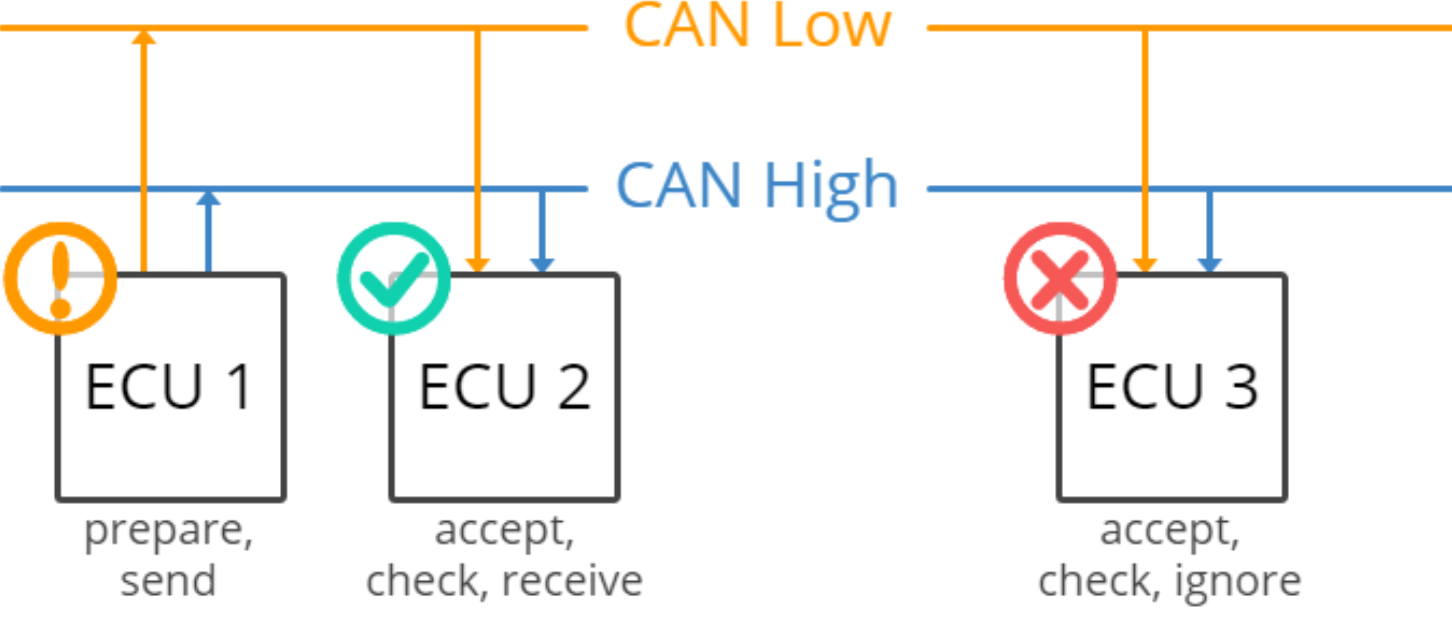
\includegraphics[width=0.5\textwidth]{Images/CAN_B.png}
	\vspace{0.2cm}
	
	% 3. La nota de la figura según APA 7 (Con la descripción técnica)
	\begin{flushleft}
		\footnotesize \textit{Nota.} Topología en bus que ilustra la interconexión en paralelo de las unidades de control electrónico compartiendo las líneas diferenciales CAN High y CAN Low. Tomado de \citep{TopeParts_EBikeProtocol}.
	\end{flushleft}
\end{figure}

\subsection{Arquitectura de la red CAN}
La implantación de este modelo de comunicaciones supuso un avance en cuanto a la cantidad de
conexiones entre dispositivos que eran necesarias para mantener todos los elementos comunicados, ya que el protocolo CAN emplea un único bus de comunicaciones, compartido por todos los dispositivos y evita la necesidad de establecer una conexión punto a punto con cada uno. Algunas de las características  que permiten a este protocolo ser adecuado para aplicaciones automotrices e industriales son:
\begin{itemize}
    \item Comunicación multi-maestro: En una red CAN no existe un nodo maestro que controle toda la comunicación. Todos los nodos conectados al bus tienen la capacidad de transmitir información cuando el canal está disponible. Esto permite una mayor flexibilidad y confiabilidad en el sistema.
    \item Comunicación basada en mensajes: A diferencia de otros protocolos de red que utilizan direcciones específicas para cada dispositivo, el bus CAN utiliza un sistema basado en identificadores de mensajes (tramas). Cada mensaje transmitido en la red contiene un identificador que indica el tipo de información que se está enviando y su nivel de prioridad. En la Figura ~\ref{fig:CAN_Frame} se presenta la estructura de datos CAN, esta cuenta de las siguientes partes:  a) Star of frame (inicio de trasmicion), b) Identifier: identificador, c) Control, d) Data (datos a transmitir), e) Cyclic Redundancy Check (detección de errores), f) Acknowledgement (confirmación) y e) End of frame (fin de trasmisión).

\begin{figure}[h]
	\centering
	
	% 1. El caption automático estilo APA 7 (Título arriba)
	\caption{Estructura de la trama de datos del protocolo CAN}
	\label{fig:CAN_Frame}
	\vspace{0.3cm}
	
	% 2. La imagen ajustada proporcionalmente al ancho del texto
	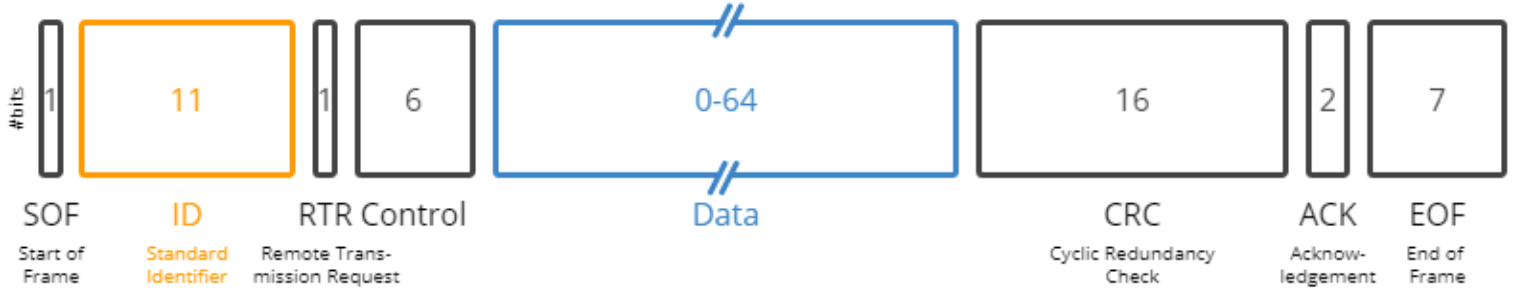
\includegraphics[width=0.9\textwidth]{Images/CAN-Frame.png}
	\vspace{0.2cm}
	
	% 3. La nota de la figura según APA 7 (Con descripción de ingeniería)
	\begin{flushleft}
		\footnotesize \textit{Nota.} Distribución de los campos de bits dentro de una trama estándar CAN, incluyendo el identificador de arbitraje, campo de control, campo de datos y el código de verificación CRC. Tomado de \citep{CarLightVision_CANBUSvsNonCANBUS}.
	\end{flushleft}
\end{figure}
    
    \item Alta inmunidad al ruido: El bus CAN utiliza una señal diferencial transmitida a través de dos líneas trenzadas denominadas CAN High y CAN Low. Esto permite reducir los efectos de interferencias electromagnéticas, lo cual es fundamental en el entorno automotriz donde existen múltiples fuentes de ruido eléctrico.
    \item Detección y manejo de errores: incluye múltiples mecanismos de detección de errores que garantizan la integridad de los datos transmitidos como: i) Verificación de redundancia cíclica (CRC); ii) Confirmación de recepción (ACK-acknowledge) y iii) Monitoreo de bits. Cuando se detecta un error, el mensaje es retransmitido automáticamente 
    
\end{itemize}

\subsection{Arquitectura física del bus CAN}
Una red CAN está compuesta por varios dispositivos denominados nodos (módulos), los cuales se conectan a un medio físico común denominado bus como se presenta en la figura ~\ref{fig:CAN_B}. Cada nodo esta compuesto principalmente por tres nodos que son:
\begin{enumerate}
    \item Microcontrolador: procesa la información del sistema y genera los datos que seran transmitidos.
    \item Controlador CAN: implementa el protocolo de comunicación CAN y gestiona la transmisión y recepción de mensajes puede estar incorporado en el microcontrolador o como un circuito externo.
    \item Transceptor CAN: convierte las señales digitales del controlador CAN en señales diferenciales que pueden transmitirse a través del bus físico.
\end{enumerate}

\section{Arquitectura física del bus CAN}
A nivel físico, el bus CAN está compuesto por una línea de comunicación diferencial formada por dos conductores. Estos dos cables transportan señales complementarias que permiten mejorar la inmunidad al ruido electromagnético. Los cables que transportan señales en protocolo CAN se identifican por ser pares trenzados como se presenta en la Figura \ref{fig:Can_Cable}.

\begin{figure}[h]
	\centering
	
	% 1. El caption automático estilo APA 7 (Título conciso arriba)
	\caption{Configuración física del cableado del protocolo CAN}
	\label{fig:Can_Cable}
	\vspace{0.3cm}
	
	% 2. La imagen con su escala original
	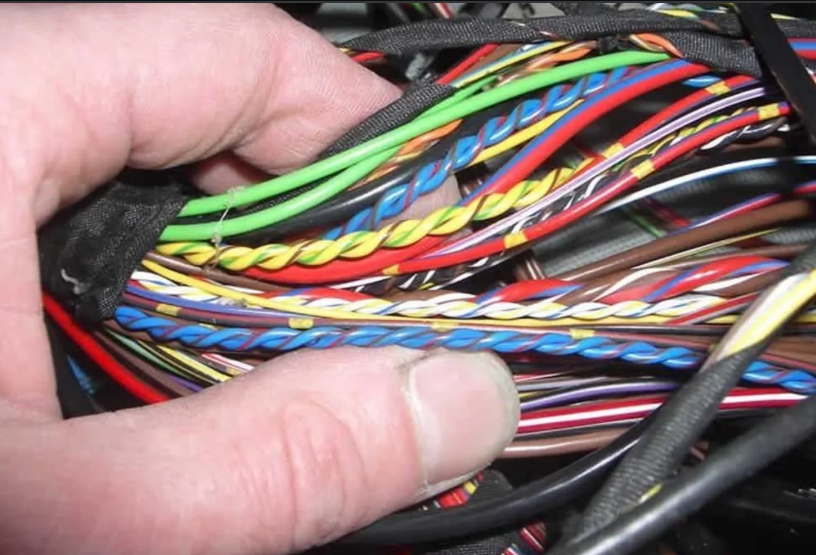
\includegraphics[width=0.6\textwidth]{Images/can cable.png}
	\vspace{0.2cm}
	
	% 3. La nota de la figura según APA 7 (Con descripción técnica)
	\begin{flushleft}
		\footnotesize \textit{Nota.} Disposición física de las líneas diferenciales de comunicación mediante par trenzado, diseñada para mitigar el ruido electromagnético en el entorno automotriz. Tomado de \citep{CarLightVision_CANBUSvsNonCANBUS}.
	\end{flushleft}
\end{figure}

El bus puede encontrarse en modo recesivo, con ambos cables con el mismo nivel de tensión o en modo dominante. En estado recesivo (inactivo), ambas líneas están cerca de 2,5V. En estado dominante (activo), CAN-H sube a 3,5V y CAN-L baja a 1,5V,Este modo de comunicación tiene como objetivo proporcionar una mayor protección frente a interferencias electromagnéticas. Esta protección viene dada, debido a que la lectura de los bits se basa en la diferencia de voltaje entre los dos cables trenzados, por lo que en caso de verse sometidas a la misma influencia electromagnética, a pesar de la variación señal en los cables, la diferencia de voltaje entre ellos se mantiene constante.

 En la Figura ~\ref{fig:Can_Volt} se presenta los niveles de voltaje de este protocolo. En el bus, los bits dominantes equivalen al nivel lógico "0", y los bits recesivos al valor lógico "1".
 
\begin{figure}[h]
	\centering
	
	% 1. El caption automático estilo APA 7 (Título conciso arriba)
	\caption{Niveles de voltaje diferencial en el bus CAN}
	\label{fig:Can_Volt}
	\vspace{0.3cm}
	
	% 2. La imagen con su escala original
	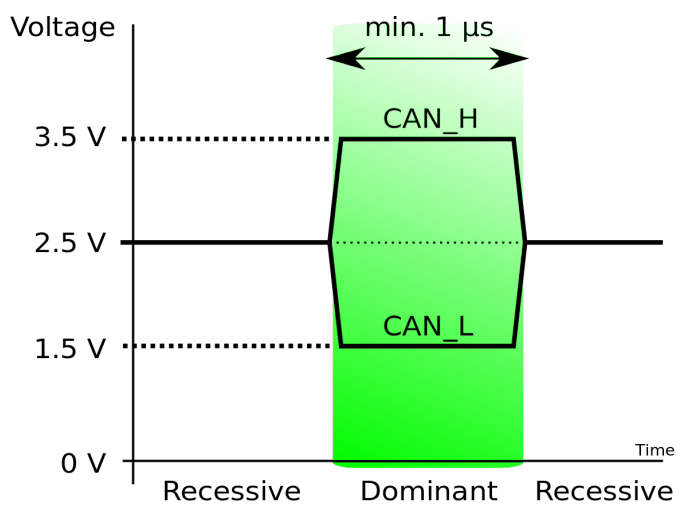
\includegraphics[width=0.6\textwidth]{Images/Can_Volt.png}
	\vspace{0.2cm}
	
	% 3. La nota de la figura según APA 7 (Con descripción técnica)
	\begin{flushleft}
		\footnotesize \textit{Nota.} Comportamiento eléctrico de las señales CAN High y CAN Low durante los estados lógicos dominante y recesivo para la transmisión física de datos. Tomado de \citep{Jidoshaseibishi_19}.
	\end{flushleft}
\end{figure}
    
\subsection{Topología del bus CAN}
Posee una topología en forma de bus, en la que únicamente son necesarios dos cables trenzados y todos los nodos se conectan a un mismo cable principal. En los extremos del bus se colocan resistencias de terminación, generalmente de 120 ohmios, con el objetivo de evitar reflexiones de señal y garantizar la estabilidad de la comunicación. \citep{Lifeder_BusTopology,IndustrialMonitorDirect_CANTermination}

La longitud máxima del bus depende de la velocidad de transmisión utilizada. Tabla \ref{bus_length} se presenta la velocidad, longitud y tiempo de transmisión  mediante este protocolo de comunicación a diferentes distancias. 

\begin{table}[h]
	\centering
	% Título separado bajo norma estricta APA 7
	\captionsetup{labelformat=simple, labelsep=newline, textfont=it, labelfont=bf}
	\caption{Relación entre longitud del bus, velocidad y tiempo máximo de transmisión}
	\label{bus_length}
	\vspace{0.3cm}
	
	% Usamos tabularx equilibrando las tres columnas uniformemente
	\begin{tabularx}{\linewidth}{X X X}
		\toprule % Línea superior APA 7
		\rowcolor[rgb]{0.851, 0.851, 0.851}
		\textbf{Longitud del bus} & \textbf{Velocidad (bits/s)} & \textbf{Tiempo máximo de transmisión} \\
		\midrule % Línea divisoria de encabezado APA 7
		Hasta 25 m & 1 Mbit/s & 129 $\mu$s \\
		\addlinespace
		Hasta 100 m & 500 Kbit/s & 258 $\mu$s \\
		\addlinespace
		Hasta 500 m & 125 Kbit/s & 1032 $\mu$s \\
		\addlinespace
		Hasta 1000 m & 50 Kbit/s & 2580 $\mu$s \\
		\bottomrule % Línea inferior de cierre APA 7
	\end{tabularx}
	\vspace{0.2cm}
	
	\begin{flushleft}
		\footnotesize \textit{Nota.} Elaboración propia.
	\end{flushleft}
\end{table}



\subsection{Tramas del protocolo CAN}
El protocolo CAN contempla diferentes formatos de tramas, cada una orientada a un propósito específico dentro del funcionamiento del protocolo en la figura ~\ref{fig:CAN_Frame} se presentan las partes mas importantes  que son:
\begin{itemize}
    \item Tramas de datos: utilizadas para el paso de información entre nodos, que puede ser  enviada y recibida por uno o varios de ellos.
    \item Tramas de error:  utilizadas cuando algún nodo de la red detecta un error en alguno de los mensajes transmitidos por otros nodos de la red conectada.
    \item Tramas de petición remota: utilizadas para solicitar el envío de información a otro nodo. Se envía una trama con el identificador (id) del nodo del que se requiere el envío de información, éste recibe la trama y devuelve la información con los datos solicitados. 
    \item Tramas de sobrecarga: utilizadas para detectar errores de sobre carga.  Es enviada por un nodo cuando éste está sobrecargado, provoca un retardo en la comunicación.
\end{itemize}

Cuando el bus esta en retardo no existe flujo de tramas y el bus se mantiene en estado recesivo. Cuando el bus requiere enviar mas de una trama estas deben estar separadas por una secuencia predeterminada (intertrama) que esta compuesta por tres bits recesivos.

Los datos enviados por este protocolo son de hasta 8 bytes. En la figigura \ref{fig:Frame} se presenta el formato de esta trama requiere 1 bit  para el inicio de la secuencia se cuenta empleado para la sincronización con el resto de la secuencia. Posteriormente se encuentra el identificador de 11 bits. Conociendo los identificadores de todas las tramas que intentan ser transmitidas, se puede establecer de manera determinista el orden en el que son transmitidas. Se puede establecer un orden para priorizar algunas tramas sobre otras por ejemplo: una trama CAN con identificador más bajo (mayor número de bits dominantes en las primeras posiciones) tiene más prioridad que una trama con identificador más alto. 

Para el campo de control los dos bits iniciales están reservados para un uso futuro, y posteriormente
se encuentran cuatro bits, que definen el tamaño del campo de datos de la trama que se encuentra a
continuación. La parte de la trama coloreada en rojo en la Figura \ref{fig:Frame} es la de datos que puede abarcar hasta 8 bytes. El campo CRC (Código de redundancia cíclica), se encarga de asegurar la integridad de los datos enviados esta cuenta con 15 bit y un bit adicional un bit recesivo como delimitador. La trama continua con 2 bits de confirmación o reconocimiento ACK (acknowledge) y finalmente se envían los bits de fin de trama EOF(end of frame) que contiene 7 bits. Adicionalmente la trama debe contener tres bits de espaciado al final de trama.

\begin{figure}[h]
	\centering
	
	% 1. El caption automático estilo APA 7 (Título conciso arriba)
	\caption{Campos constitutivos del formato de trama de datos CAN}
	\label{fig:Frame}
	\vspace{0.3cm}
	
	% 2. La imagen ajustada proporcionalmente al ancho del texto
	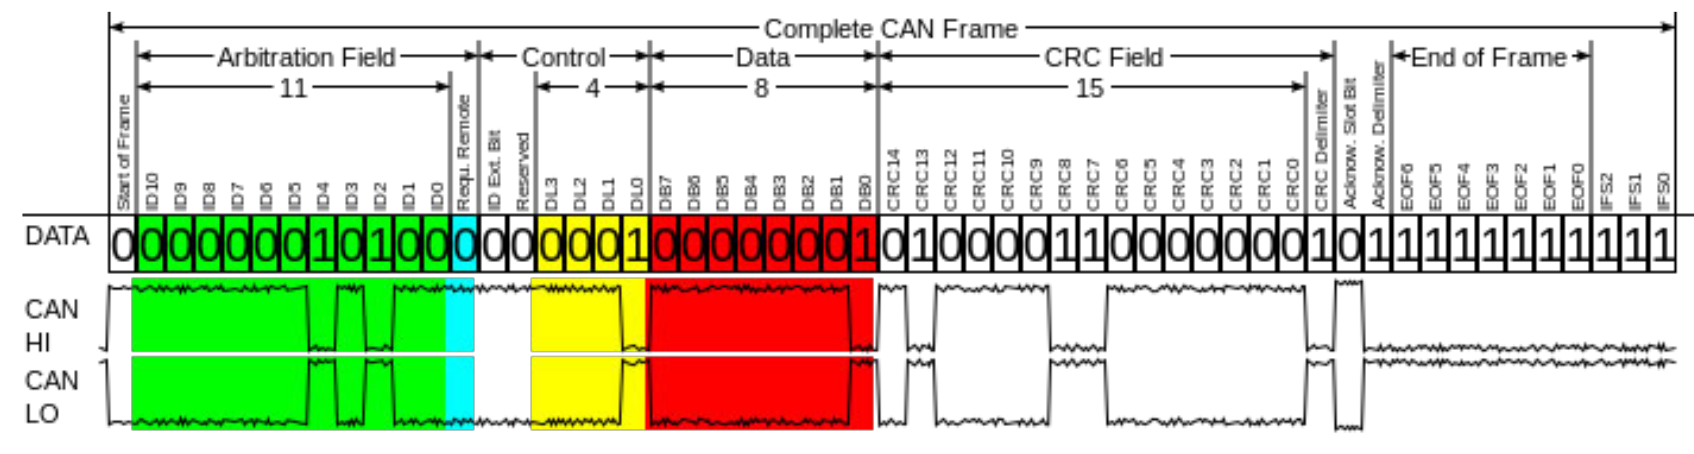
\includegraphics[width=0.9\textwidth]{Images/Frame.png}
	\vspace{0.2cm}
	
	% 3. La nota de la figura según APA 7 (Con descripción técnica)
	\begin{flushleft}
		\footnotesize \textit{Nota.} Segmentación detallada del formato de la trama estándar, especificando la longitud y función de los bits de inicio, arbitraje, control, datos, CRC, ACK y fin de trama (*EOF*). Tomado de \citep{Jeong_Ch7VehicleNetwork}.
	\end{flushleft}
\end{figure} 

\subsection{Errores en trama de datos}

El protocolo CAN posee una norma de relleno de bits en las tramas, que consiste en que cada secuencia de cinco bits con el mismo valor, se introduce un bit de valor inverso. Esto provoca que el formato de las tramas de error incumplan esta norma y puedan ser detectadas sobre las tramas de datos. Estas tramas de error pueden ser generadas por cualquier nodo que detecte un error en la comunicación. Se componen de dos campos. Se compone de dos campos primero se encuentra el indicador de error, o error flag, cuyo formato depende el tipo de nodo que haya detectado el error. En la Figura \ref{fig:Errorp}, se describen las partes de esta trama. 


\begin{figure}[h]
	\centering
	
	% 1. El caption automático estilo APA 7 (Título conciso arriba)
	\caption{Estructura de una trama de error en el protocolo CAN}
	\label{fig:Errorp}
	\vspace{0.3cm}
	
	% 2. La imagen ajustada proporcionalmente al ancho del texto
	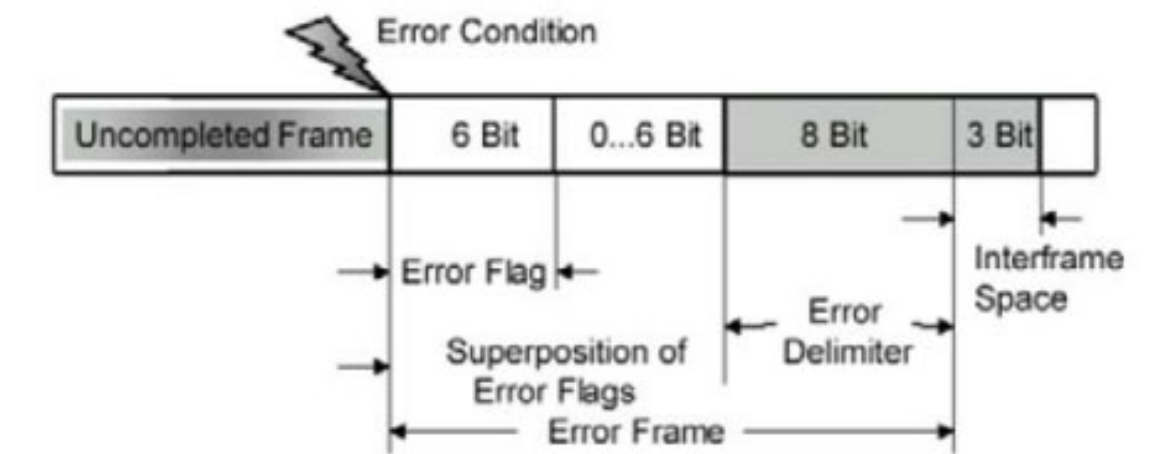
\includegraphics[width=0.8\textwidth]{Images/Error.png}
	\vspace{0.2cm}
	
	% 3. La nota de la figura según APA 7 (Con descripción técnica)
	\begin{flushleft}
		\footnotesize \textit{Nota.} Configuración de los campos de la trama de error, detallando los bits de delimitación y la secuencia de banderas de error activas o pasivas utilizadas para la gestión de fallas en el bus. Tomado de \citep{NCKU_EmbeddedWiki}.
	\end{flushleft}
\end{figure}

Para evitar que un nodo con errores condicione el funcionamiento de la red o pueda provocar fallos o saturaciones, el protocolo dispone de medidas para desconectar de la red este tipo de nodos. Los nodos pueden estar en tres tipos de estado diferente que son:
\begin{itemize}
    \item Error activo: El nodo puede enviar mensajes y tramas de error normalmente. Es el estado normal.
    \item Error pasivo: El nodo cambia el formato de sus tramas de error, enviando 12 bits recesivos. De este modo, el resto de nodos no son capaces de detectarlas y no ralentiza las comunicaciones.
    \item Bus off o Anulado: El nodo se auto-desconecta del bus, se deshabilita su transceptor y no participa en la comunicación.
\end{itemize}

Cuando un nodo se desconecta de la red, se resetea, configura y se conecta de nuevo a la red, pero no podrá comenzar a transmitir de nuevo hasta no haber recibido 128 secuencias de 11 bits recesivos sin errores en el bus.
\subsection{Red CAN en vehículos}

La red CAN (\textit{Controller Area Network}) es uno de los protocolos de comunicación más utilizados en vehículos modernos debido a su capacidad para permitir la comunicación entre múltiples unidades de control electrónico (ECU) mediante un bus compartido. A través de esta red, distintos módulos del vehículo intercambian información relacionada con el motor, transmisión, frenos, sistemas de seguridad y otros subsistemas electrónicos \citep{Flexihub_OBD2, CISE_CAN}. 

En los sistemas OBD-II modernos, especialmente aquellos basados en el protocolo ISO 15765-4, la comunicación de diagnóstico se realiza sobre la red CAN utilizando identificadores específicos para solicitudes y respuestas. Generalmente, las herramientas de diagnóstico envían solicitudes mediante el identificador funcional 0x7DF, mientras que las ECU responden utilizando identificadores comprendidos entre 0x7E8 y 0x7EF \citep{Flexihub_OBD2}. Mediante este mecanismo es posible consultar parámetros estandarizados conocidos como PIDs (\textit{Parameter IDs}), los cuales permiten obtener datos como velocidad del vehículo, revoluciones del motor, temperatura del refrigerante o flujo de aire del motor.

Sin embargo, además de los PIDs normalizados definidos por el estándar OBD-II, los fabricantes implementan protocolos CAN propietarios para la comunicación interna entre las ECU del vehículo. Estos mensajes no se encuentran documentados públicamente y varían dependiendo de la marca, modelo y año del vehículo. Debido a ello, gran parte de la información transmitida en la red CAN no puede ser interpretada directamente sin realizar procesos de ingeniería inversa (\textit{reverse engineering}) \citep{Flexihub_OBD2, CAN_D_2020}.

La ingeniería inversa sobre redes CAN consiste en capturar y analizar las tramas transmitidas por las ECU con el objetivo de identificar qué mensajes corresponden a determinados parámetros del vehículo. Para ello, normalmente se registra el tráfico CAN mientras se modifica una variable específica del vehículo, por ejemplo acelerar, activar luces o mover el volante. Posteriormente se analizan los identificadores CAN y los bytes de datos que presentan variaciones relacionadas con dicha acción \citep{reddit_CAN_reverse, embedded_CAN_reverse}. 

Un aspecto importante en el análisis de tramas CAN es la interpretación de los datos binarios transmitidos por las ECU. Cada mensaje CAN contiene una secuencia de bytes que representan información específica del vehículo, la cual debe convertirse desde formato hexadecimal o binario a valores numéricos comprensibles conocidos como DBC \citep{Flexihub_OBD2}. 

\subsection{Archivo DBC CAN}

Un archivo CAN DBC (CAN Database) es un archivo de texto que contiene la información necesaria para decodificar los datos sin procesar transmitidos por la red CAN y convertirlos en valores físicos interpretables. Este tipo de archivo define la estructura de los mensajes y de las señales asociadas, permitiendo establecer cómo debe leerse cada dato dentro de una trama CAN.

La Figura \ref{fig:dbc_sintaxis} presenta la estructura básica de un mensaje y de una señal dentro de un archivo DBC. Este tipo de archivo se utiliza para describir la forma en que los datos transmitidos a través de la red CAN deben ser interpretados, permitiendo asociar los valores binarios con variables físicas de interés.

\begin{figure}[htbp]
	\centering
	
	% 1. El caption automático estilo APA 7 (Título arriba)
	\caption{Sintaxis básica de un mensaje y una señal en un archivo DBC}
	\label{fig:dbc_sintaxis}
	\vspace{0.3cm}
	
	% 2. La imagen ajustada proporcionalmente al ancho del texto
	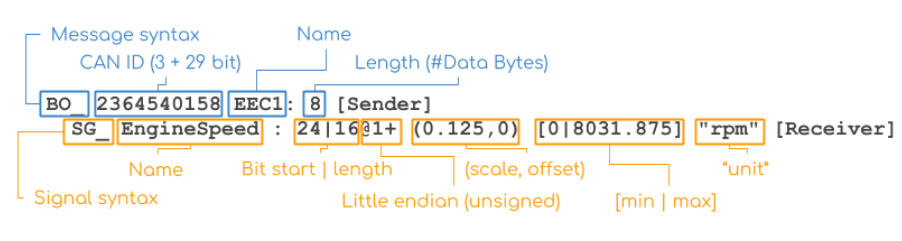
\includegraphics[width=0.9\textwidth]{Images/BDC.png}
	\vspace{0.2cm}
	
	% 3. La nota de la figura según APA 7 (Con descripción técnica)
	\begin{flushleft}
		\footnotesize \textit{Nota.} Estructura de codificación en bases de datos CAN (*.dbc*), donde se definen los identificadores de los mensajes (BO\_), los nombres de las señales (SG\_), el orden de los bits (*endianness*), el factor de escala y el offset de conversión. Elaboración propia.
	\end{flushleft}
\end{figure}

En la parte superior de la figura se muestra la sintaxis correspondiente a un mensaje, identificada con el prefijo \texttt{BO\_}. En esta definición se incluye el identificador CAN, el nombre del mensaje, la longitud expresada en número de bytes de datos y el nodo transmisor. Estos elementos permiten describir de manera ordenada cada trama que circula por el bus CAN.

En la parte inferior se presenta la sintaxis de una señal, indicada mediante el prefijo \texttt{SG\_}. En este caso, se especifica el nombre de la señal, la posición inicial del bit, la longitud de la señal, el orden de bytes, el tipo de dato, el factor de escala, el desplazamiento, el rango físico, la unidad de medida y el nodo receptor. La combinación de estos parámetros define cómo debe interpretarse cada señal contenida dentro de un mensaje.

Por ejemplo, en la señal mostrada en la figura, \texttt{EngineSpeed} corresponde al nombre de la señal; \texttt{24|16} indica que la señal inicia en el bit 24 y tiene una longitud de 16 bits; \texttt{@1+} señala una codificación little-endian y un dato sin signo; \texttt{(0.125,0)} representa el factor de escala y el desplazamiento; \texttt{[0|8031.875]} define el rango físico de la señal, y \texttt{rpm} establece la unidad de medida.

En este sentido, el archivo DBC funciona como una guía de decodificación que permite transformar los datos crudos del bus CAN en magnitudes físicas comprensibles, tales como velocidad, régimen del motor, temperatura o presión. Por ello, constituye una herramienta fundamental en aplicaciones de diagnóstico automotriz, monitoreo de variables vehiculares, telemetría e ingeniería inversa de redes CAN.

Un ejemplo simplificado de sintaxis DBC para la velocidad del vehículo es el siguiente:\\

\begin{verbatim}
	BO_ 2024 OBD2: 8 Vector__XXX
	SG_ VehicleSpeed : 0|8@1+ (1,0) [0|255] "km/h" Vector__XXX
\end{verbatim}

En este ejemplo, \texttt{VehicleSpeed} es el nombre de la señal, \texttt{0|8} indica que la señal comienza en el bit 0 y tiene una longitud de 8 bits, \texttt{@1+} señala que usa little-endian y que es no firmada, \texttt{(1,0)} corresponde al factor de escala y al desplazamiento, \texttt{[0|255]} define el rango físico permitido, \texttt{"km/h"} representa la unidad y \texttt{Vector\_\_XXX} actúa como nodo genérico.

Por ejemplo, una trama CAN correspondiente a una respuesta OBD-II puede representarse de la siguiente manera:

\begin{center}
	\texttt{7E8 03 41 0D 37 FF FF FF FF}
\end{center}

En esta trama, \texttt{7E8} corresponde al identificador de respuesta de la ECU, \texttt{41} indica una respuesta positiva al modo de diagnóstico 01, \texttt{0D} representa el PID de velocidad del vehículo y \texttt{37} contiene el valor de la señal. Al convertir \texttt{37} de hexadecimal a decimal se obtiene 55, por lo que la velocidad interpretada es de \texttt{55 km/h}.

De esta manera, los archivos DBC permiten transformar datos CAN sin procesar en variables físicas útiles para aplicaciones de monitoreo vehicular, diagnóstico automotriz, telemetría e ingeniería inversa de redes CAN.

%-------------------------2.5----------------


	\section{Sistema de inyección electrónica}
\subsection{Evolución de los sistemas de alimentación de combustible}


La evolución de los sistemas de alimentación de combustible en los vehículos ha pasado desde el carburador mecánico hasta sistemas electrónicos de inyección monopunto, multipunto e inyección directa, cada uno asociado a cambios normativos sobre emisiones y avances en electrónica del motor\citep{web1,web10,web14}.

\begin{itemize}
    \item \textbf{Finales del siglo XIX -- 1900}:  
    Los primeros motores de gasolina utilizan mezcladores mecánicos rudimentarios; el carburador se consolida como dispositivo estándar para crear la mezcla aire–combustible\citep{web10, web14}.

    \item \textbf{1912 -- 1930s}:  
    Primeros ensayos de bombas de inyección de gasolina en motores de aviación; en 1937 se aplica en serie la inyección de combustible en motores de avión, sentando las bases para los sistemas de inyección modernos\citep{web14}.

    \item \textbf{1945 -- 1950s}:  
    Primera aplicación en serie de inyección de gasolina en vehículos de carretera; se mantienen sistemas principalmente mecánicos o electromecánicos, usados en modelos deportivos o de alta gama\citep{web14}.

    \item \textbf{1967}:  
    Bosch introduce el sistema D‑Jetronic, el primer sistema de inyección electrónica de gasolina de producción masiva, sustituyendo parcialmente al carburador en Europa\citep{web1}.

    \item \textbf{1970s}:  
    La crisis del petróleo y las normas de emisiones obligan a abandonar parcialmente el carburador; se extienden sistemas de inyección electrónica continuos (por ejemplo KE‑Jetronic) y se empiezan a usar en modelos de serie de fabricantes como Mercedes‑Benz y otros\citep{web1,web14}.

    \item \textbf{1980s}:  
    Aparecen sistemas digitales de gestión del motor (por ejemplo Motronic de Bosch), integrando inyección electrónica multipunto y encendido electrónico; marcas como Volkswagen, BMW y Mercedes adoptan estos sistemas en múltiples modelos\citep{web7}.

    \item \textbf{1990}:  
    Se difunden sistemas de inyección electrónica monopunto y multipunto indirecta en vehículos comerciales de bajo costo (por ejemplo Suzuki Samurai 1990 y Suzuki Jimny 2000)\citep{web10}.

    \item \textbf{1990s -- 2000s}:  
    Implantación masiva del carburador en motores de gasolina reemplazado por inyección electrónica multipunto (por ejemplo General Motors, Ford, Honda, etc.); se adopta el catalizador de tres vías, lo que exige un control muy preciso de la mezcla aire–combustible\citep{web1,web7,web10}.

    \item \textbf{2000s -- 2010s}:  
    Desarrollo de sistemas de inyección directa de gasolina (GDI) en modelos de alta eficiencia y potencia (por ejemplo Toyota, Mazda, BMW, VW, GM); se combinan turbocompresores y control electrónico avanzado para reducir consumo y emisiones\citep{web1,web7}.

    \item \textbf{2010 -- actualidad}:  
    La inyección directa se vuelve estándar en muchos motores de gasolina y se introducen sistemas flexibles de inyección múltiple por ciclo, combinados con sistemas híbridos y electrificación parcial de la alimentación (bomba eléctrica de alta presión, inyección piezoeléctrica en diesel)\citep{web1,web7}.
\end{itemize}

\begin{figure}[h]
	\centering
	
	% 1. El caption automático estilo APA 7 (Título conciso arriba)
	\caption{Línea de tiempo de la evolución en los sistemas de alimentación de combustible}
	\label{fig:evolucion_combustible}
	\vspace{0.3cm}
	
	% 2. La imagen ajustada exactamente al límite del margen del texto
	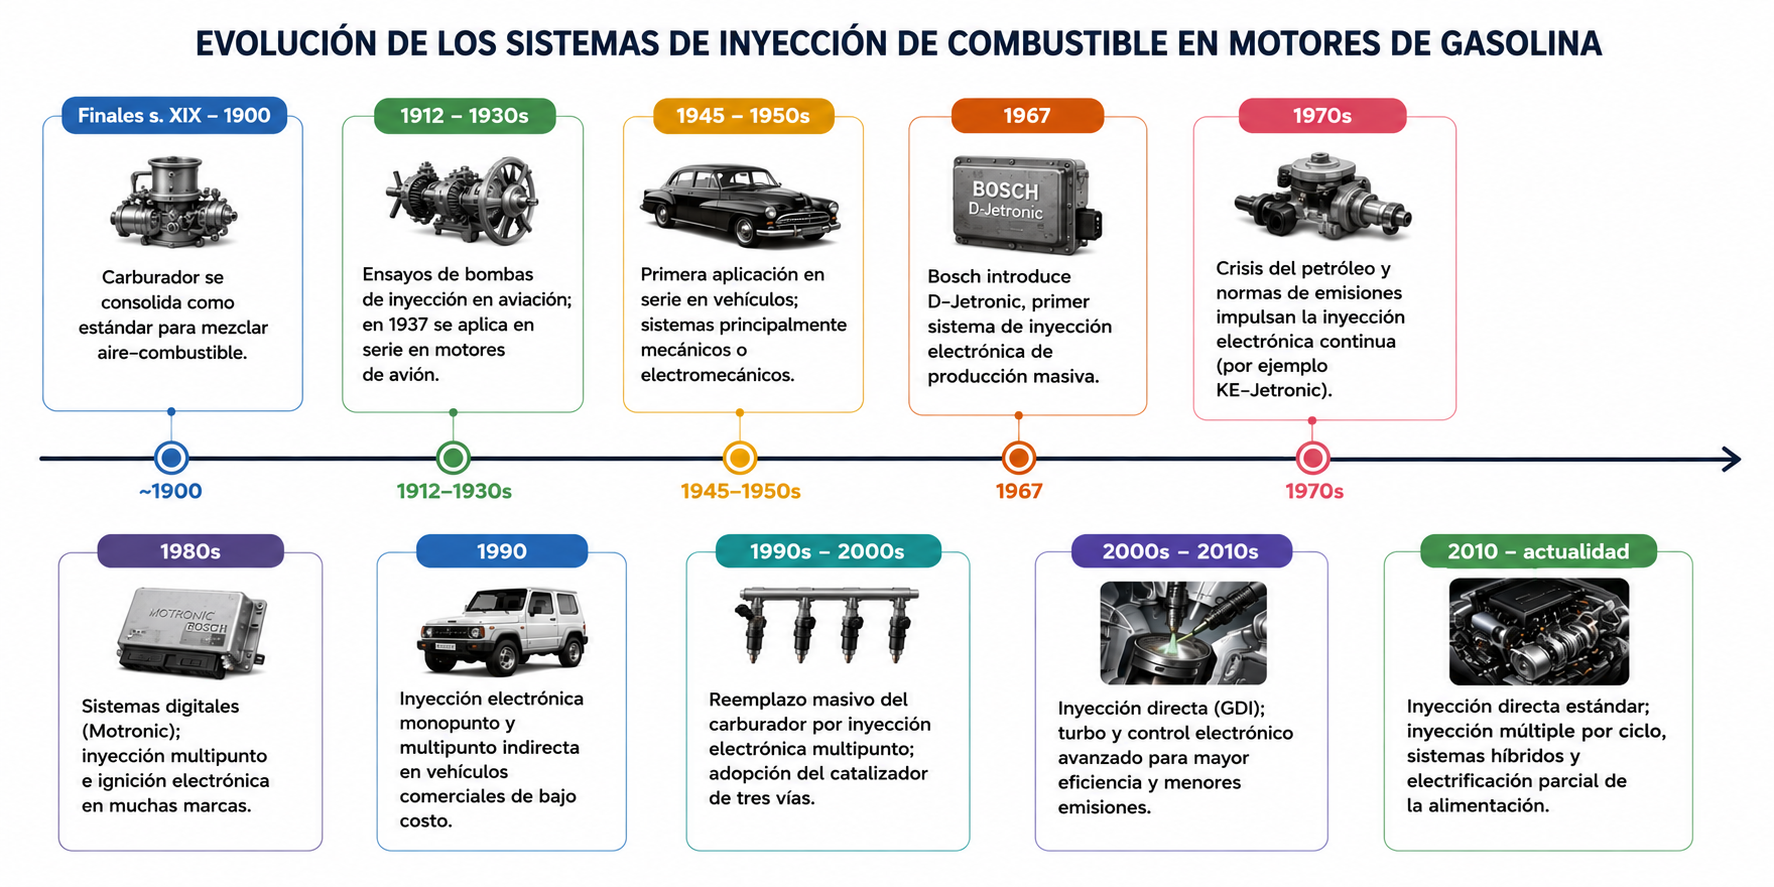
\includegraphics[width=1.0\textwidth]{Images/LINEA.png}
	\vspace{0.2cm}
	
	% 3. La nota de la figura según APA 7 (Con descripción técnica)
	\begin{flushleft}
		\footnotesize \textit{Nota.} Cronología del desarrollo tecnológico en la dosificación de combustible, destacando la transición desde sistemas mecánicos por carburador hasta esquemas de inyección electrónica directa controlados por computadora. Elaboración propia con base en \citep{web1}, \citep{web10} y \citep{web7}.
	\end{flushleft}
\end{figure}

\subsection{Tipos de sistemas de inyección electrónica}% (monopunto, multipunto, directa)

Los sistemas de inyección electrónica pueden clasificarse según la forma en que suministran el combustible hacia el motor. Entre los más utilizados se encuentran la inyección monopunto, multipunto y directa, cada una con diferentes características de funcionamiento, eficiencia y complejidad tecnológica \citep{Bosch_Automotive, web_inyeccion1}.

\subsubsection{Inyección monopunto}

La inyección monopunto, también conocida como \textit{Single Point Injection} (SPI) o \textit{Throttle Body Injection} (TBI), utiliza un único inyector ubicado en el cuerpo de aceleración para suministrar combustible a todos los cilindros del motor. Su funcionamiento es similar al carburador, pero con control electrónico de la dosificación de combustible \citep{Bosch_Automotive}.

Este sistema fue ampliamente utilizado durante la transición entre carburadores y sistemas de inyección electrónica modernos debido a su bajo costo y simplicidad. Sin embargo, presenta menor precisión en la distribución del combustible y menor eficiencia energética en comparación con sistemas más avanzados \citep{web_inyeccion2}.

Entre sus principales ventajas se encuentran:
\begin{itemize}
    \item Menor costo de implementación.
    \item Diseño simple y mantenimiento reducido.
    \item Mejor control de emisiones respecto al carburador.
\end{itemize}

No obstante, sus desventajas incluyen:
\begin{itemize}
    \item Distribución desigual del combustible.
    \item Menor rendimiento y eficiencia.
    \item Mayor consumo comparado con sistemas modernos.
\end{itemize}

\subsubsection{Inyección multipunto}

La inyección multipunto o \textit{Multi Point Injection} (MPI) emplea un inyector independiente para cada cilindro del motor. Los inyectores se encuentran ubicados en el múltiple de admisión, permitiendo una dosificación más precisa de combustible hacia cada cilindro \citep{Bosch_Automotive, web_inyeccion1}.

Este sistema mejora significativamente el rendimiento del motor, el consumo de combustible y las emisiones contaminantes. Dependiendo de la estrategia de control de la ECU, la inyección puede realizarse de forma simultánea, secuencial o semisecuencial \citep{web_inyeccion2}.

Entre sus ventajas destacan:
\begin{itemize}
    \item Mejor atomización y distribución del combustible.
    \item Reducción del consumo y emisiones.
    \item Mayor eficiencia y respuesta del motor.
\end{itemize}

Sin embargo:
\begin{itemize}
    \item Requiere mayor cantidad de sensores y componentes electrónicos.
    \item Presenta mayor complejidad de diagnóstico y mantenimiento.
\end{itemize}

\subsubsection{Diferencia entre monopunto y multipunto}
De acuerdo con Motorpasión, la inyección directa puede considerarse una evolución de la inyección multipunto, debido a que ambos sistemas utilizan un inyector por cilindro, pero difieren principalmente en la ubicación donde se introduce el combustible. En la inyección multipunto, el combustible es suministrado en el colector de admisión antes de ingresar a la cámara de combustión ver Figura \ref{fig:Multi}, mientras que en la inyección directa el combustible es pulverizado directamente dentro del cilindro, permitiendo una combustión más eficiente y un mejor aprovechamiento energético \citep{Motorpasion_Inyeccion}.

\begin{figure}[h]
	\centering
	
	% 1. El caption automático estilo APA 7 (Título conciso arriba)
	\caption{Diferencias estructurales entre los sistemas de inyección monopunto y multipunto}
	\label{fig:Multi}
	\vspace{0.3cm}
	
	% 2. La imagen ajustada proporcionalmente al ancho del texto
	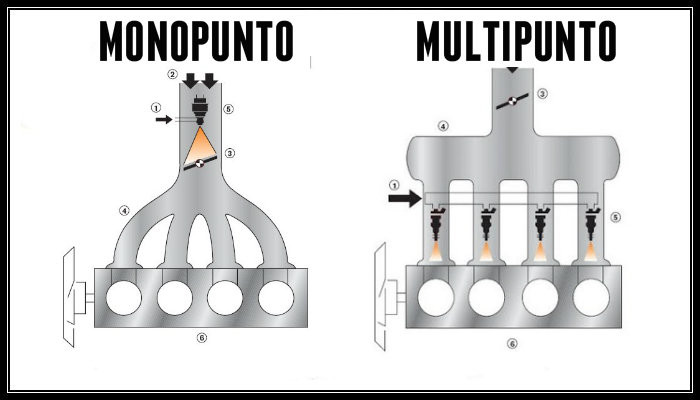
\includegraphics[width=0.6\textwidth]{Images/MULTI.jpg}
	\vspace{0.2cm}
	
	% 3. La nota de la figura según APA 7 (Con descripción técnica)
	\begin{flushleft}
		\footnotesize \textit{Nota.} Comparación esquemática del posicionamiento y cantidad de inyectores en la galería de admisión, contrastando el suministro centralizado (monopunto) frente al flujo independiente por cilindro (multipunto). Tomado de \citep{Motorpasion_Inyeccion}.
	\end{flushleft}
\end{figure}

\subsubsection{Inyección directa}

La inyección directa de gasolina o \textit{Gasoline Direct Injection} (GDI) introduce el combustible directamente dentro de la cámara de combustión a alta presión, eliminando el paso previo por el múltiple de admisión \citep{Bosch_GDI, web_inyeccion3}.

Este sistema permite un control mucho más preciso de la mezcla aire-combustible, incrementando la eficiencia térmica del motor y reduciendo el consumo de combustible. Además, puede trabajar junto con turbocompresores y estrategias avanzadas de \mbox{control electrónico \citep{Bosch_GDI}}.

Entre sus principales ventajas se encuentran:
\begin{itemize}
    \item Mayor eficiencia energética.
    \item Mejor desempeño y potencia.
    \item Reducción de emisiones contaminantes.
\end{itemize}

Como desventajas:
\begin{itemize}
    \item Mayor complejidad electrónica y mecánica.
    \item Costos elevados de mantenimiento.
    \item Sensibilidad a la calidad del combustible.
\end{itemize}


A continuacion en la Tabla \ref{tab:INye} se compara los distintos tipos de sistemas de inyección electrónica.

\begin{table}[h]
	\centering
	% Título separado bajo norma estricta APA 7
	\captionsetup{labelformat=simple, labelsep=newline, textfont=it, labelfont=bf}
	\caption{Comparación entre los tipos de sistemas de inyección electrónica}
	\label{tab:INye}
	\vspace{0.3cm}
	
	% Se usa tabularx para un autoajuste milimétrico a los márgenes
	\begin{tabularx}{\linewidth}{p{3.8cm} X X X}
		\toprule % Línea superior APA 7
		\rowcolor[rgb]{0.851, 0.851, 0.851}
		\textbf{Característica} & \textbf{Inyección monopunto} & \textbf{Inyección multipunto} & \textbf{Inyección directa} \\
		\midrule % Línea divisoria de encabezado APA 7
		Cantidad de inyectores & Un solo inyector para todos los cilindros & Un inyector por cilindro & Un inyector por cilindro \\
		\addlinespace
		Ubicación de inyección & Cuerpo de aceleración & Colector de admisión & Dentro de la cámara de combustión \\
		\addlinespace
		Formación de mezcla & Antes del múltiple de admisión & Antes de ingresar al cilindro & Dentro del cilindro \\
		\addlinespace
		Precisión de dosificación & Baja & Media-Alta & Alta \\
		\addlinespace
		Consumo de combustible & Mayor & Moderado & Menor \\
		\addlinespace
		Eficiencia energética & Baja & Buena & Muy alta \\
		\addlinespace
		Complejidad electrónica & Baja & Media & Alta \\
		\bottomrule % Línea inferior de cierre APA 7
	\end{tabularx}
	\vspace{0.2cm}
	
	\begin{flushleft}
		\footnotesize \textit{Nota.} Elaboración propia con base en~\citep{Motorpasion_Inyeccion}, \citep{Bosch_Automotive} y~\citep{Bosch_GDI}.
	\end{flushleft}
\end{table}

Actualmente, la inyección directa es ampliamente utilizada en vehículos modernos debido a sus ventajas en eficiencia, desempeño y cumplimiento de normativas ambientales \citep{Bosch_GDI, web_inyeccion3}.



\subsection{Componentes principales del sistema de inyección}% (inyectores, bomba, regulador, sensores)


El sistema de inyección electrónica está conformado por diversos componentes encargados de suministrar, regular y controlar la cantidad de combustible necesaria para el correcto funcionamiento del motor. Estos elementos trabajan de manera conjunta bajo la supervisión de la unidad de control electrónico (ECU), permitiendo optimizar el rendimiento, el consumo de combustible y las emisiones contaminantes \citep{Bosch_Automotive, Bosch_GDI}.

\subsubsection{Inyectores}

Los inyectores son dispositivos electromecánicos encargados de pulverizar el combustible hacia el múltiple de admisión o directamente dentro de la cámara de combustión, dependiendo del tipo de sistema de inyección utilizado. Su funcionamiento es controlado electrónicamente por la ECU mediante pulsos eléctricos que determinan el tiempo de apertura y la cantidad de combustible inyectada \citep{Bosch_GDI}.

La correcta atomización del combustible es fundamental para lograr una combustión eficiente, reducir emisiones contaminantes y mejorar el desempeño del motor. En sistemas modernos de inyección directa, los inyectores trabajan a altas presiones y permiten múltiples inyecciones por ciclo de combustión.

Entre las principales funciones de los inyectores se encuentran:
\begin{itemize}
    \item Dosificar la cantidad de combustible requerida.
    \item Pulverizar el combustible en partículas finas.
    \item Mejorar la mezcla aire-combustible.
    \item Reducir consumo y emisiones.
\end{itemize}

\subsubsection{Bomba de combustible}

La bomba de combustible tiene la función de suministrar el combustible desde el tanque hacia los inyectores manteniendo una presión adecuada dentro del sistema. En vehículos modernos generalmente se utiliza una bomba eléctrica ubicada dentro del tanque de combustible \citep{web_bomba_combustible}.

La presión generada por la bomba depende del tipo de sistema de inyección. Los sistemas multipunto trabajan con presiones moderadas, mientras que los sistemas de inyección directa requieren bombas de alta presión capaces de alimentar los inyectores directamente en la cámara de combustión.

Entre sus funciones principales destacan:
\begin{itemize}
    \item Transportar combustible desde el tanque.
    \item Mantener presión constante en el sistema.
    \item Garantizar el suministro adecuado al motor.
\end{itemize}

\subsubsection{Regulador de presión}

El regulador de presión es el componente encargado de mantener estable la presión del combustible dentro del riel de inyectores ver Figura \ref{fig:Inye}, evitando variaciones que puedan afectar la mezcla aire-combustible \citep{Bosch_Automotive}.

Cuando la presión excede el valor establecido, el regulador permite el retorno del exceso de combustible hacia el tanque. En sistemas modernos, esta regulación puede realizarse electrónicamente mediante sensores y módulos de control integrados.

Sus principales funciones son:
\begin{itemize}
    \item Estabilizar la presión de combustible.
    \item Proteger inyectores y conductos.
    \item Garantizar una dosificación precisa.
\end{itemize}


\begin{figure}[h]
	\centering
	
	% 1. El caption automático estilo APA 7 (Título conciso arriba)
	\caption{Componentes principales y distribución del sistema de inyección electrónica}
	\label{fig:Inye}
	\vspace{0.3cm}
	
	% 2. La imagen ajustada proporcionalmente al ancho del texto
	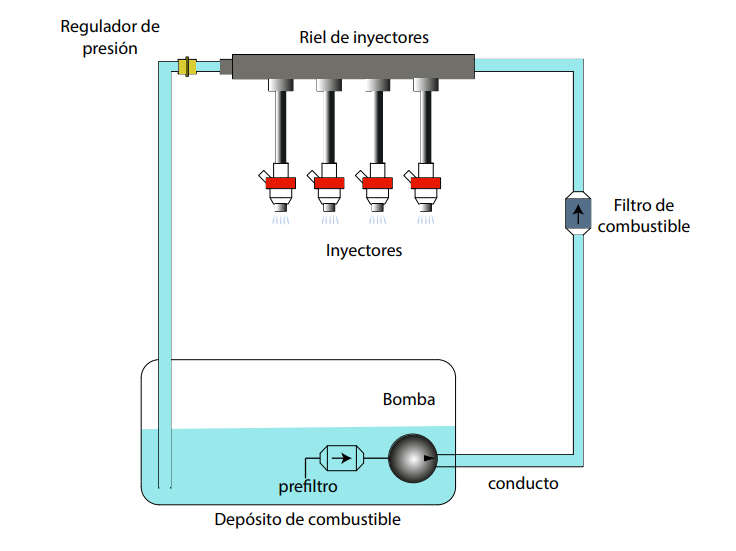
\includegraphics[width=0.9\textwidth]{Images/sistema.png}
	\vspace{0.2cm}
	
	% 3. La nota de la figura según APA 7 (Con descripción técnica)
	\begin{flushleft}
		\footnotesize \textit{Nota.} Disposición física y conectividad de los elementos constitutivos del sistema, incluyendo unidades de control, sensores de monitoreo de parámetros y actuadores para la dosificación de combustible. Elaboración propia con base en~\citep{Fundamentos_Inyeccion}.
	\end{flushleft}
\end{figure}
    
    
\subsubsection{Sensores}

Los sensores son dispositivos encargados de medir diferentes variables de funcionamiento del motor y enviar esta información a la ECU para que pueda calcular la cantidad exacta de combustible necesaria en cada condición de operación \citep{Bosch_Automotive, web_sensores_motor}.

Entre los sensores más importantes del sistema de inyección electrónica se encuentran:
\begin{itemize}
    \item Sensor MAF (\textit{Mass Air Flow}): mide el flujo de aire que ingresa al motor.
    \item Sensor MAP (\textit{Manifold Absolute Pressure}): mide la presión del múltiple de admisión.
    \item Sensor TPS (\textit{Throttle Position Sensor}): detecta la posición de la mariposa de aceleración.
    \item Sensor ECT (\textit{Engine Coolant Temperature}): mide la temperatura del refrigerante.
    \item Sensor de oxígeno o lambda: controla la cantidad de oxígeno presente en los gases de escape.
\end{itemize}

La información proporcionada por estos sensores permite que la ECU ajuste continuamente la mezcla aire-combustible, optimizando el rendimiento del motor y reduciendo emisiones contaminantes.


\subsection{Control de la mezcla aire-combustible}

El control de la mezcla aire-combustible constituye uno de los procesos fundamentales en los sistemas modernos de inyección electrónica, debido a su influencia directa sobre la eficiencia térmica del motor, el consumo de combustible y la formación de emisiones contaminantes durante la combustión \citep{Fundamentos_Inyeccion, Bosch_GDI}.

La mezcla aire-combustible se define como la proporción entre la masa de aire y la masa de combustible que ingresa al cilindro para llevar a cabo el proceso de combustión. En motores a gasolina, la relación estequiométrica ideal se aproxima a 14,7:1, es decir, 14,7 partes de aire por cada parte de combustible \citep{Bosch_Automotive}. Esta condición permite una combustión más eficiente y favorece el funcionamiento adecuado del convertidor catalítico.

Para evaluar la calidad de la mezcla, se utiliza el factor lambda ($\lambda$), definido como:

\begin{equation}
	\lambda = \frac{(A/F)_{\mathrm{real}}}{(A/F)_{\mathrm{estequiometrico}}}
	\label{eq:lambda}
\end{equation}

Donde $(A/F)_{\mathrm{real}}$ representa la relación aire-combustible presente en el motor y $(A/F)_{\mathrm{estequiometrico}}$ corresponde a la relación ideal para la combustión completa.

Las variaciones del factor lambda afectan de manera significativa tanto las emisiones contaminantes como el desempeño del motor. Las mezclas ricas incrementan la emisión de monóxido de carbono (CO) e hidrocarburos no quemados (HC), mientras que las mezclas pobres pueden favorecer la formación de óxidos de nitrógeno (NO$_x$) y provocar una disminución de la potencia entregada por el motor \citep{Combustion_Emissions_2020}.

El control de esta mezcla es realizado por la unidad de control electrónico (ECU), la cual recibe información de distintos sensores del motor para ajustar de forma continua el tiempo de inyección y mantener condiciones de combustión adecuadas. Entre los sensores más relevantes se encuentran el sensor MAF, el sensor MAP, el sensor TPS, el sensor ECT y, de manera especial, el sensor de oxígeno o sensor lambda, encargado de medir la concentración de oxígeno presente en los gases de escape \citep{Bosch_Automotive, Fundamentos_Inyeccion}.

A partir de la señal proporcionada por el sensor lambda, la ECU puede implementar un control en lazo cerrado (\textit{closed loop}), mediante el cual corrige de forma dinámica la cantidad de combustible inyectado para mantener el valor de $\lambda$ cercano a 1. Este mecanismo mejora la eficiencia del motor, reduce el consumo de combustible y contribuye a la disminución de las emisiones contaminantes \citep{Bosch_GDI}.

Finalmente, diversos estudios han demostrado que un control preciso de la mezcla aire-combustible tiene un impacto significativo en la reducción de emisiones vehiculares y en la optimización del desempeño energético de los motores de combustión interna. En este sentido, el desarrollo de estrategias avanzadas de control electrónico ha permitido mejorar el funcionamiento del motor bajo diferentes condiciones de carga, velocidad y operación \citep{Combustion_Emissions_2020}.

\subsection{Relación del sistema de inyección con el consumo de combustible}

El sistema de inyección electrónica tiene una relación directa con el consumo de combustible, debido a que la cantidad de combustible suministrada al motor depende del tiempo de apertura del inyector. En este contexto, la duración del pulso de inyección constituye una variable fundamental para estimar el consumo instantáneo, ya que representa el tiempo durante el cual el inyector permanece abierto y permite el paso del combustible hacia la cámara de combustión \citep{article2020fuelconsumption}.

De acuerdo con el artículo de referencia, el consumo instantáneo puede determinarse a partir de la medición de la duración del pulso de inyección, estableciéndose una correlación muy alta entre ambas variables, con un coeficiente de 0,99 \cite{article2020fuelconsumption}. Esto indica que, al incrementarse el ancho del pulso, aumenta también la cantidad de combustible inyectado; por el contrario, una reducción del tiempo de apertura disminuye el caudal de combustible y, en consecuencia, el consumo del motor \citep{article2020fuelconsumption}.

\begin{figure}[h]
	\centering
	
	% 1. El caption automático estilo APA 7 (Título conciso arriba)
	\caption{Relación entre el sistema de inyección y el consumo de combustible}
	\label{fig:sistema_inyeccion}
	\vspace{0.3cm}
	
	% 2. La imagen ajustada proporcionalmente al ancho del texto
	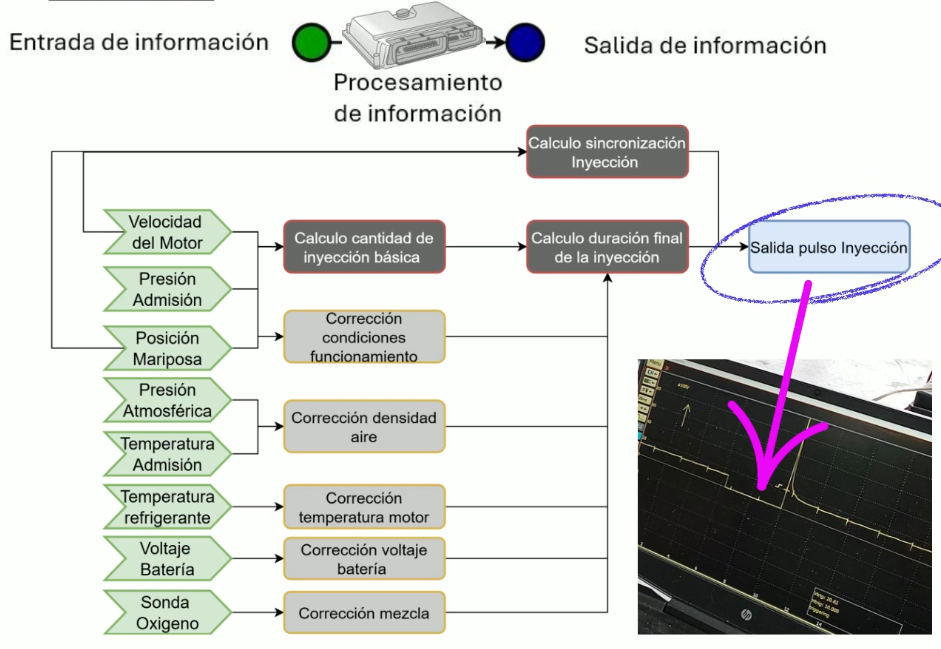
\includegraphics[width=0.9\textwidth]{Images/combu.png}
	\vspace{0.2cm}
	
	% 3. La nota de la figura según APA 7 (Con descripción técnica)
	\begin{flushleft}
		\footnotesize \textit{Nota.} Diagrama de bloques que ilustra cómo los parámetros medidos por la ECU (tiempo de inyección y flujo de masa de aire) impactan en el cálculo matemático del consumo instantáneo de combustible. Tomado de~\citep{Youtube_Inyeccion_2024}.
	\end{flushleft}
\end{figure}

La Figura \ref{fig:sistema_inyeccion} ilustra el proceso de adquisición y procesamiento de señales dentro del sistema de gestión del motor, donde las variables de entrada son procesadas por la unidad de control hasta generar la salida hacia el inyector. En particular, la señal de salida del pulso de inyección es el parámetro que permite regular la mezcla aire-combustible y, por tanto, influye de manera directa en el gasto de combustible durante la operación del motor \citep{article2020fuelconsumption}.

Por ello, el análisis del pulso de inyección resulta útil para estudiar el comportamiento real del motor bajo diferentes condiciones de operación, así como para evaluar estrategias orientadas a mejorar la eficiencia energética y reducir el consumo específico de combustible \citep{article2020fuelconsumption}.
%-------------------------2.6----------------
\section{Modelos matemáticos para el consumo del combustible}
\subsection{Concepto de consumo de combustible}

El consumo de combustible se define como la cantidad de combustible que utiliza un motor o vehículo para desarrollar un recorrido o mantener su operación durante un periodo determinado. Este parámetro constituye una de las variables más importantes en el análisis del desempeño automotriz, debido a que refleja de manera directa la eficiencia energética del sistema de propulsión y su impacto económico y ambiental \citep{PosadaHenao2016, EstimacionAlgoritmoUPS}.

Desde el punto de vista técnico, el consumo puede expresarse en términos de volumen o masa de combustible por unidad de distancia recorrida, como litros por cada 100 km (L/100 km), o por unidad de tiempo, como litros por hora (L/h), dependiendo del tipo de evaluación que se requiera \citep{PosadaHenao2016}. En motores de combustión interna, este indicador no solo depende de la demanda de potencia, sino también de las condiciones de operación del vehículo, tales como la velocidad, la carga, la pendiente del terreno, la resistencia aerodinámica y el estado del sistema de inyección \citep{ConsumoVehiculos2002, PosadaHenao2016}.

En términos generales, un menor consumo de combustible se asocia con una mejor eficiencia del motor, siempre que se mantengan condiciones adecuadas de potencia y funcionamiento. Sin embargo, este comportamiento puede variar en función de la estrategia de control del motor, la calidad de la combustión y las características del trayecto o ciclo de conducción \citep{EstimacionAlgoritmoUPS, ConsumoVehiculos2002}.

Por esta razón, el estudio del consumo de combustible constituye una base fundamental para el desarrollo de modelos matemáticos que permitan estimar, comparar y optimizar el desempeño de los motores en diferentes condiciones de operación \citep{PosadaHenao2016}.

\subsection{Métodos de estimación del consumo}

La estimación del consumo de combustible ha sido abordada mediante distintos enfoques matemáticos y experimentales, cuyo objetivo principal es determinar con precisión la cantidad de combustible utilizada por un vehículo durante su operación. En términos generales, estos métodos pueden clasificarse en modelos basados en variables de conducción, modelos fundamentados en parámetros del motor y modelos estadísticos o híbridos que combinan distintas señales del sistema vehicular \citep{EstimacionConsumoTransporte2004, EstimacionAlgoritmoUPS}.

Los modelos basados en variables de conducción utilizan información como la velocidad, la distancia recorrida, la aceleración y las condiciones de operación del vehículo para aproximar el consumo. Este tipo de enfoque resulta útil cuando no se dispone de acceso directo a variables internas del motor, aunque su precisión puede verse limitada por las variaciones propias del ciclo de conducción y por la topografía de la ruta \citep{ConsumoVehiculos2002, EstimacionConsumoTransporte2004}.

Por otro lado, los modelos basados en parámetros del motor emplean señales obtenidas desde la unidad de control electrónico o mediante el puerto OBD-II, tales como el flujo másico de aire (MAF), la posición del acelerador (TPS), las revoluciones por minuto (RPM) y la relación aire-combustible. Estos modelos presentan una mayor capacidad de representación del comportamiento real del motor, ya que incorporan variables directamente relacionadas con la formación de la mezcla y la entrega de combustible \citep{MAFFuelConsumption2024, ResearchOBD2018}.

Adicionalmente, existen métodos estadísticos y de aprendizaje automático que permiten construir relaciones empíricas entre variables de operación y consumo de combustible. Aunque estos enfoques pueden ofrecer buenos niveles de predicción, requieren bases de datos representativas y procesos de calibración adecuados para asegurar su validez en diferentes condiciones de uso \citep{EstimatingRegression2018, ResearchOBD2018}.

En este contexto en la Tabla \ref{tab:estim} se muestra, la selección del método de estimación depende de la disponibilidad de datos, el nivel de precisión requerido y la complejidad aceptable del modelo . Para aplicaciones en tiempo real, los modelos basados en sensores como el MAF representan una alternativa adecuada, debido a que permiten relacionar directamente la masa de aire admitida por el motor con la cantidad de combustible necesaria para mantener una combustión eficiente \citep{MAFFuelConsumption2024, Bosch_GDI}.

\begin{table}[h]
	\centering
	% Título separado bajo norma estricta APA 7
	\captionsetup{labelformat=simple, labelsep=newline, textfont=it, labelfont=bf}
	\caption{Comparación de métodos para la estimación del consumo de combustible}
	\label{tab:estim}
	\vspace{0.3cm}
	
	% Usamos tabularx para una distribución fluida y equilibrada de las columnas
	\begin{tabularx}{\linewidth}{p{2.5cm} X X X}
		\toprule % Línea superior APA 7
		\rowcolor[rgb]{0.851, 0.851, 0.851}
		\textbf{Método} & \textbf{Principio} & \textbf{Ventajas} & \textbf{Limitaciones} \\
		\midrule % Línea divisoria de encabezado APA 7
		Estadístico & Relaciona consumo con variables observables como velocidad o distancia. & Simple y económico. & Menor precisión en condiciones variables. \\
		\addlinespace
		Mecanicista & Usa fuerzas resistivas y demanda de potencia del vehículo. & Más físico y explicativo. & Requiere mayor cantidad de parámetros y calibración. \\
		\addlinespace
		Basado en sensores & Utiliza señales directas de la ECU como MAF, MAP, TPS o sonda lambda. & Ideal para la estimación y monitoreo en tiempo real. & Depende de la tasa de refresco y calidad de los sensores. \\
		\bottomrule % Línea inferior de cierre APA 7
	\end{tabularx}
	\vspace{0.2cm}
	
	\begin{flushleft}
		\footnotesize \textit{Nota.} Elaboración propia.
	\end{flushleft}
\end{table}

\subsection{Relación aire-combustible (AFR)}

La relación aire-combustible, conocida como \textit{Air-Fuel Ratio} (AFR), expresa la proporción existente entre la masa de aire y la masa de combustible que ingresan al cilindro durante el proceso de combustión. Este parámetro es fundamental en el análisis del funcionamiento de los motores de combustión interna, ya que determina la calidad de la mezcla y condiciona directamente la eficiencia térmica, el consumo de combustible y la generación de emisiones contaminantes \citep{AFRLambdaHPAcademy, AFRAnsed}.

En motores a gasolina, la relación estequiométrica de referencia es aproximadamente 14.7:1, lo que significa que se requieren 14.7 partes de aire por cada parte de combustible para lograr una combustión ideal \citep{AFRLambdaHPAcademy, Bosch_Automotive}. Bajo esta condición, el combustible puede oxidarse de manera más completa y se favorece el funcionamiento adecuado de los sistemas de postratamiento, como el convertidor catalítico.

Cuando la relación aire-combustible es inferior a la estequiométrica, la mezcla se considera rica, debido al exceso de combustible presente en la cámara de combustión. En este caso, aumenta la probabilidad de generar monóxido de carbono (CO) e hidrocarburos no quemados (HC), debido a una combustión incompleta \citep{AFRAnsed}. Por el contrario, cuando la relación aire-combustible es superior a la estequiométrica, la mezcla es pobre, lo que implica un exceso de aire. Esta condición puede disminuir el consumo de combustible, pero también puede afectar la potencia del motor y favorecer la formación de óxidos de nitrógeno (NO$_x$) \citep{AFRLambdaHPAcademy, Combustion_Emissions_2020}.

\begin{figure}[h]
	\centering
	
	% 1. El caption automático estilo APA 7 (Título conciso arriba)
	\caption{Curva estequiométrica del factor lambda y respuesta del sensor de oxígeno}
	\label{fig:factor_lambda}
	\vspace{0.3cm}
	
	% 2. La imagen ajustada proporcionalmente al ancho del texto
	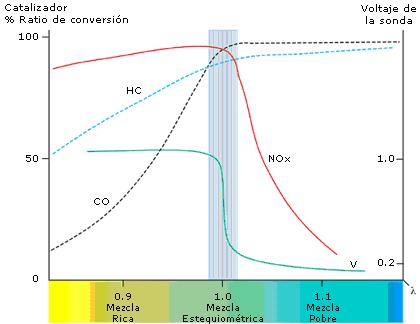
\includegraphics[width=0.75\textwidth]{Images/Sonda.JPG}
	\vspace{0.2cm}
	
	% 3. La nota de la figura según APA 7 (Con descripción técnica)
	\begin{flushleft}
		\footnotesize \textit{Nota.} Comportamiento de la señal de voltaje generada por el sensor de oxígeno en función del factor lambda, detallando las regiones de transición entre mezcla rica y mezcla pobre. Adaptado de~\citep{Fundamentos_Inyeccion}.
	\end{flushleft}
\end{figure}

La AFR está estrechamente relacionada con el factor lambda ($\lambda$), el cual permite expresar qué tan lejos se encuentra la mezcla real respecto de la condición estequiométrica ver Tabla \ref{tab:afr} En términos generales, el control de la AFR constituye una estrategia esencial para mantener una combustión eficiente y adaptar la entrega de combustible a las condiciones de carga, velocidad y demanda del motor \citep{Bosch_GDI, Fundamentos_Inyeccion}.

Para el cálculo final del consumo, es fundamental definir la relación aire-combustible ($AFR$), la cual se expresa como la proporción entre la masa de aire y la masa de combustible:

\begin{equation}
	AFR = \frac{m_{aire}}{m_{combustible}}
\end{equation}

En los sistemas de gestión modernos, esta relación se normaliza mediante el factor $\lambda$ (lambda), que relaciona el $AFR$ real medido por la sonda de oxígeno con el valor estequiométrico ideal:

\begin{equation}
	\lambda = \frac{AFR_{real}}{AFR_{estequiometrico}}
\end{equation}

Si $\lambda = 1$, la mezcla es estequiométrica; si $\lambda < 1$, la mezcla es rica (exceso de combustible), y si $\lambda > 1$, la mezcla es pobre (exceso de aire) ver Figura \ref{fig:factor_lambda}.

Por esta razón, el análisis de la relación aire-combustible es indispensable dentro de los modelos matemáticos de estimación del consumo de combustible, ya que permite vincular la cantidad de aire admitida con la masa de combustible requerida para sostener una operación eficiente del motor.

\begin{table}[htbp]
	\centering
	% Título separado bajo norma estricta APA 7
	\captionsetup{labelformat=simple, labelsep=newline, textfont=it, labelfont=bf}
	\caption{Interpretación de la relación aire-combustible y el factor lambda}
	\label{tab:afr}
	\vspace{0.3cm}
	
	% Usamos tabularx para un autoajuste milimétrico a los márgenes
	\begin{tabularx}{\linewidth}{p{3.8cm} p{2.8cm} p{2.2cm} X}
		\toprule % Línea superior APA 7
		\rowcolor[rgb]{0.851, 0.851, 0.851}
		\textbf{Condición} & \textbf{Relación AFR} & \textbf{Factor $\lambda$} & \textbf{Efecto principal y aplicación} \\
		\midrule % Línea divisoria de encabezado APA 7
		\textbf{Mezcla rica} & AFR $<$ 14,7:1 & $\lambda < 1$ & Mayor consumo de combustible y aumento de emisiones de CO y HC. Típica en aceleraciones a plena carga. \\
		\addlinespace
		\textbf{Mezcla estequiométrica} & AFR = 14,7:1 & $\lambda = 1$ & Combustión completa y eficiente, operación óptima del catalizador. Condición ideal de crucero. \\
		\addlinespace
		\textbf{Mezcla pobre} & AFR $>$ 14,7:1 & $\lambda > 1$ & Menor consumo de combustible, incremento de temperatura en la cámara y emisiones de NOx. \\
		\bottomrule % Línea inferior de cierre APA 7
	\end{tabularx}
	\vspace{0.2cm}
	
	\begin{flushleft}
		\footnotesize \textit{Nota.} Comportamiento físico-químico de la dosificación de la mezcla aire-combustible en motores de gasolina y su impacto en la eficiencia y emisiones. Elaboración propia.
	\end{flushleft}
\end{table}

\subsection{Modelo basado en el sensor MAF}

El sensor MAF (\textit{Mass Air Flow}) es uno de los sensores más importantes dentro de los sistemas modernos de inyección electrónica, debido a que permite medir la cantidad de aire que ingresa al motor. Esta información es utilizada por la unidad de control electrónico (ECU) para calcular la cantidad adecuada de combustible necesaria para mantener una combustión eficiente \citep{Bosch_Automotive, Fundamentos_Inyeccion}. 

El funcionamiento del sensor MAF se basa generalmente en el principio de hilo caliente (\textit{Hot Wire}). En este sistema, un filamento metálico es calentado eléctricamente a una temperatura constante. Cuando el aire atraviesa el conducto de admisión, enfría el filamento y provoca una variación en la corriente eléctrica necesaria para mantener la temperatura estable. La ECU interpreta esta variación como una medida del flujo de aire que entra al motor \citep{Hella_MAF, Bosch_GDI}.

La información proporcionada por el sensor MAF permite mejorar el control de la mezcla aire–combustible, optimizar el consumo de combustible y reducir emisiones contaminantes. Además, este sensor es ampliamente utilizado en estrategias de monitoreo y diagnóstico automotriz debido a que el flujo de aire está directamente relacionado con la cantidad de combustible consumida por el motor \citep{Fundamentos_Inyeccion}.

La Figura \ref{fig:maf_sensor} muestra la ubicación típica y el principio de funcionamiento de un sensor MAF dentro del sistema de admisión del motor.

\begin{figure}[h]
	\centering
	
	% 1. El caption automático estilo APA 7 (Título descriptivo arriba)
	\caption{Principio de funcionamiento eléctrico y térmico del sensor MAF}
	\label{fig:maf_sensor}
	\vspace{0.3cm}
	
	% 2. La imagen ajustada proporcionalmente al ancho del texto
	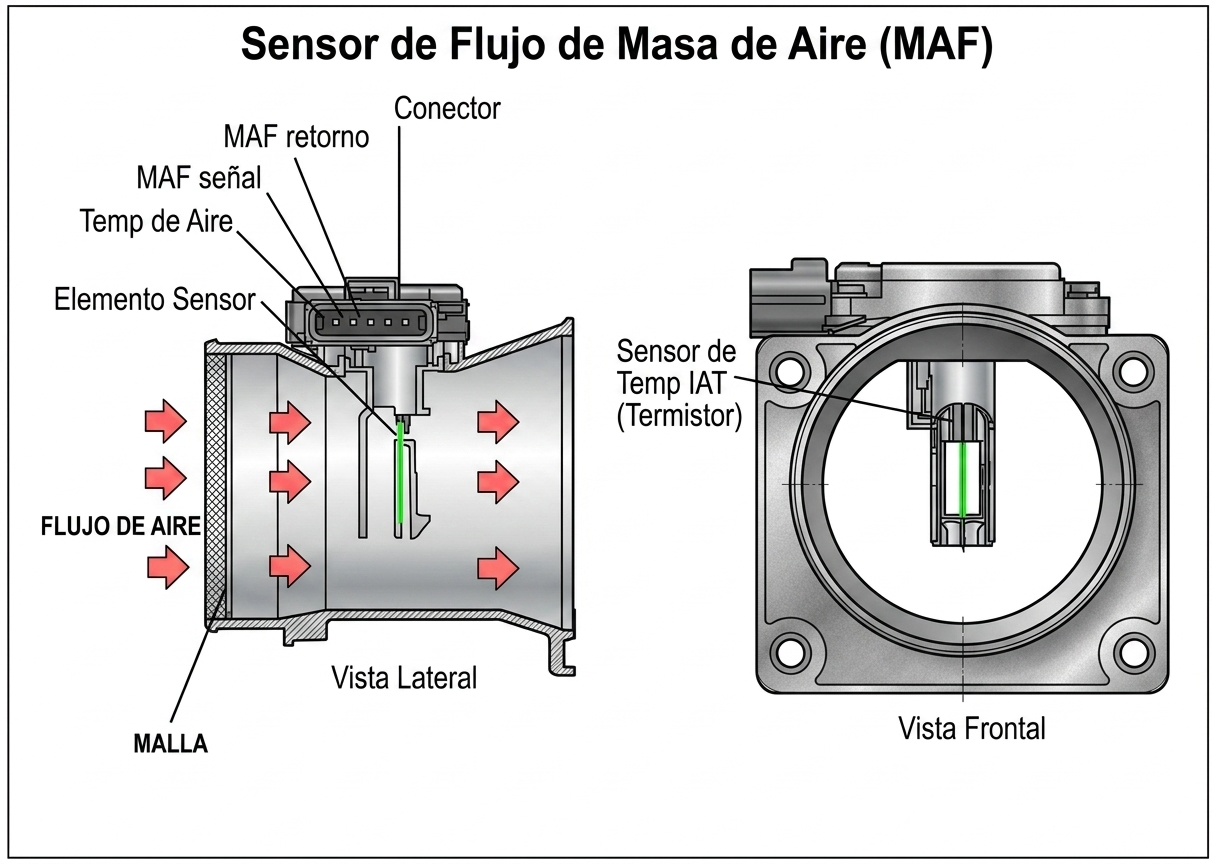
\includegraphics[width=0.75\textwidth]{Images/maf_sensor.png}
	\vspace{0.2cm}
	
	% 3. La nota de la figura según APA 7 (Con descripción técnica)
	\begin{flushleft}
		\footnotesize \textit{Nota.} Diagrama del comportamiento del flujo de masa de aire sobre el elemento térmico (hilo caliente), ilustrando cómo la transferencia de calor altera la resistencia eléctrica y la señal de salida hacia la ECU. Adaptado de~\citep{Hella_MAF}.
	\end{flushleft}
\end{figure}


Uno de los métodos más utilizados para estimar el consumo de combustible en tiempo real consiste en emplear directamente la señal del sensor MAF. Este enfoque se basa en la relación estequiométrica aire–combustible, considerando que para motores a gasolina la mezcla ideal es aproximadamente 14,7:1 \citep{Bosch_Automotive}.

El consumo de combustible puede calcularse mediante la siguiente expresión:

\begin{equation}
	FuelConsumption_{(L/h)} = \frac{MAF_{(g/s)} \times 3600}{14.7 \times 745}
\end{equation}

En esta expresión, los valores constantes representan:
\begin{itemize}
	\item \textbf{3600}: Factor de conversión de segundos a horas.
	\item \textbf{14.7}: Relación aire-combustible estequiométrica ideal para la gasolina.
	\item \textbf{745}: Densidad aproximada de la gasolina en $g/L$ (este valor puede oscilar entre $720$ y $775$ $g/L$ según la temperatura y el octanaje).
\end{itemize}

donde:

Para el cálculo operativo en motores a gasolina, se asumen valores estándar que permiten simplificar la monitorización en tiempo real. En este modelo, se consideran las siguientes constantes:

\begin{equation}
	AFR_{estequiometrico} = 14.7
\end{equation}

\begin{equation}
	\rho_{fuel} \approx 750 \, \mathrm{g/L}
\end{equation}

Es importante destacar que la densidad de la gasolina es una variable sensible a la composición química, el porcentaje de aditivos y las condiciones ambientales. En el contexto de \textbf{Bolivia}, la gasolina comercial incorpora mezclas de bioetanol (como la Gasolina Especial Plus o la Súper Etanol), lo que puede generar variaciones en la densidad y en el poder calorífico respecto a las gasolinas convencionales puras \citep{ANH_Gasolina_87}.

Sustituyendo estos valores en la fórmula general, la ecuación de consumo instantáneo se simplifica mediante un factor de conversión aproximado:

\begin{equation}
	FuelConsumption_{(L/h)} \approx MAF_{(g/s)} \times 0.33
\end{equation}

\subsection{Ejemplo de Cálculo Instantáneo}

Para ilustrar la sensibilidad del modelo, se propone el siguiente escenario: si el sistema (vía sensores MAP+IAT o MAF) registra un flujo de masa de aire de $10 \, g/s$, el consumo instantáneo se calcula como:

\begin{equation}
	FuelConsumption = \frac{10 \times 3600}{14.7 \times 745}
\end{equation}

\begin{equation}
	FuelConsumption \approx 3.29 \, \mathrm{L/h}
\end{equation}

Este resultado permite al sistema de gestión o al usuario final visualizar el gasto volumétrico de combustible en función de la carga del motor en un momento determinado.

Este modelo permite obtener estimaciones relativamente precisas del consumo instantáneo de combustible utilizando únicamente información proveniente del sistema OBD-II. Debido a su simplicidad y facilidad de implementación, es ampliamente utilizado en aplicaciones de telemetría, monitoreo vehicular y análisis de eficiencia energética \citep{CSSElectronics_OBD2, Hella_MAF}.

En el presente proyecto, este modelo constituye una de las principales estrategias para estimar el consumo de combustible en tiempo real mediante la adquisición de datos desde la ECU del vehículo a través del protocolo OBD-II.


\subsection{El Método Speed-Density: Origen y Evolución}

El modelo basado en los sensores MAP e IAT es técnicamente denominado el método \textbf{Speed-Density} (Velocidad-Densidad). Recibe este nombre porque el flujo de masa de aire no se mide directamente, sino que se infiere a partir de la \textit{velocidad} del motor (RPM) y la \textit{densidad} del aire en el colector de admisión.


Aunque el concepto de densidad de gases se remonta a la termodinámica clásica, su aplicación en el control electrónico de motores (ECU) fue impulsada por la necesidad de cumplir con las normativas de emisiones contaminantes en la década de 1970.

Uno de los pioneros en la implementación masiva de sistemas electrónicos basados en presión de vacío fue la compañía Bendix Corporation con su sistema Electrojector, y posteriormente Bosch con el sistema D-Jetronic(donde la "D" proviene del alemán Druck, que significa presión).

Este sistema fue revolucionario porque reemplazó los carburadores mecánicos por una unidad de control analógica que leía la presión del colector (MAP) para determinar el pulso de inyección. A diferencia del sistema \textit{L-Jetronic} (que usa flujo de aire directo o MAF), el sistema \textit{D-Jetronic} sentó las bases del algoritmo Speed-Density moderno.

El nombre deriva directamente de las dos variables fundamentales que la computadora del motor utiliza para consultar sus mapas de combustible:

\begin{enumerate}
	\item \textbf{Speed (Velocidad):} Se refiere a la velocidad angular del motor ($N$ en RPM). Esta variable determina la frecuencia con la que los cilindros "bombean" aire hacia adentro.
	\item \textbf{Density (Densidad):} Calculada mediante la presión (MAP) y la temperatura (IAT). La densidad ($\rho$) nos dice cuánta masa de aire hay en un volumen determinado de espacio en el colector.
\end{enumerate}

La relación fundamental del método establece que la masa de aire por cilindro ($m_{cyl}$) es proporcional a la densidad del aire en el colector multiplicada por el volumen del cilindro y corregida por la eficiencia volumétrica:

\begin{equation}
	m_{cyl} = \eta_v(N, P) \cdot \rho_{intake} \cdot V_{cyl}
\end{equation}


El uso de Speed-Density sobre otros métodos (como MAF) tiene implicaciones técnicas importantes:

\begin{itemize}
	\item \textbf{Robustez Mecánica:} Los sensores MAP son extremadamente duraderos y no obstruyen el flujo de aire, a diferencia de los hilos calientes de los sensores MAF que pueden ensuciarse.
	\item \textbf{Respuesta Transitoria:} En motores con turbocompresores de alto rendimiento, el método Speed-Density suele ser más rápido para reaccionar a cambios súbitos de presión.
	\item \textbf{Dependencia de la Calibración:} La mayor desventaja es que el sistema "no sabe" si el motor ha sido modificado (por ejemplo, levas más agresivas). Cualquier cambio físico requiere recalibrar la tabla de eficiencia volumétrica ($\eta_v$) en la ECU, ya que el cálculo es puramente matemático y no una medición física directa del aire.
\end{itemize}



\subsection{Densidad del combustible}

La densidad del combustible es una propiedad física que relaciona la masa de un fluido con el volumen que ocupa. En el caso de los combustibles líquidos, esta magnitud es relevante porque influye en la energía contenida por unidad de volumen, en el caudal inyectado y en la estimación del consumo de combustible. Por esta razón, en los ensayos de calidad de carburantes se suele reportar la densidad en condiciones normalizadas de temperatura, generalmente a 15,6$^\circ$C o 20$^\circ$C, con el fin de garantizar la comparabilidad de los resultados \citep{ANH2014, FuelsDensityToolbox}.

A nivel del mar y en condiciones normalizadas de laboratorio, la densidad de la gasolina suele ubicarse aproximadamente entre 0,71 y 0,78 g/cm$^3$, mientras que en el diésel se encuentra en un rango aproximado de 0,82 a 0,85 g/cm$^3$, aunque estos valores pueden variar según la formulación, los aditivos y la temperatura de medición \citep{FuelsDensityToolbox}. En consecuencia, una misma masa de combustible puede ocupar distinto volumen dependiendo de su densidad, lo cual afecta la forma en que se expresa y compara el consumo en términos volumétricos.

En la práctica, la densidad del combustible disminuye cuando aumenta la temperatura, debido a la expansión térmica del líquido. Por ello, los organismos técnicos y las normas de control de calidad establecen valores de referencia y métodos estandarizados de medición, como D-1298 y D-4052, para asegurar que los resultados no dependan de variaciones ambientales durante el ensayo \citep{ANH2014}.

En la ciudad de La Paz, Bolivia, la evaluación de combustibles debe considerarse dentro de un contexto de altitud elevada, cercana a 3600 m. s. n. m., donde la presión atmosférica es menor que a nivel del mar \citep{BarometricaPaz}. Aunque la densidad del combustible como propiedad intrínseca no depende directamente de la altitud, las condiciones ambientales de operación del motor sí influyen en el comportamiento de la combustión y en la estimación real del consumo, por lo que resulta necesario trabajar con valores corregidos o medidos bajo condiciones controladas \citep{ANH2014}.

En la Tabla \ref{tab:densidad} se presenta valores aproximados de algunos carburantes utilizados en sistemas de combustión interna.


\begin{table}[h]
	\centering
	% Título separado bajo norma estricta APA 7
	\captionsetup{labelformat=simple, labelsep=newline, textfont=it, labelfont=bf}
	\caption{Densidad típica de combustibles líquidos a temperatura de referencia}
	\label{tab:densidad}
	\vspace{0.3cm}
	
	% Usamos tabularx para una distribución fluida y adaptativa
	\begin{tabularx}{\linewidth}{p{3.5cm} p{4.5cm} X}
		\toprule % Línea superior APA 7
		\rowcolor[rgb]{0.851, 0.851, 0.851}
		\textbf{Combustible} & \textbf{Densidad aproximada} & \textbf{Observación} \\
		\midrule % Línea divisoria de encabezado APA 7
		Gasolina & 0,715 -- 0,780 g/cm$^{3}$ & Varía según la formulación estacional y la temperatura. \\
		\addlinespace
		Diésel & 0,820 -- 0,845 g/cm$^{3}$ & Presenta mayor densidad y contenido energético que la gasolina. \\
		\addlinespace
		Jet fuel & 0,775 -- 0,840 g/cm$^{3}$ & Sujeto a especificaciones y normativas internacionales aeronáuticas. \\
		\addlinespace
		GLP & Variable & Altamente dependiente de la proporción de la mezcla propano-butano. \\
		\bottomrule % Línea inferior de cierre APA 7
	\end{tabularx}
	\vspace{0.2cm}
	
	\begin{flushleft}
		\footnotesize \textit{Nota.} Valores de referencia utilizados para la conversión volumétrica en el cálculo de tasas de consumo masivo en sistemas de combustión interna. Elaboración propia.
	\end{flushleft}
\end{table}

En este sentido, la densidad del combustible constituye una variable de apoyo dentro de los modelos matemáticos de consumo, especialmente cuando se desea convertir el caudal volumétrico a caudal másico o cuando se analizan diferencias de desempeño entre distintas zonas geográficas.

\subsection{Efecto de la altura en el consumo de gasolina}

La altura sobre el nivel del mar influye de manera significativa en el desempeño de los motores de combustión interna, debido a que al aumentar la altitud disminuyen la presión atmosférica y la densidad del aire. Esta reducción implica una menor cantidad de oxígeno disponible por unidad de volumen, lo que afecta directamente el proceso de combustión y la potencia desarrollada por el motor \citep{LopezRuano2018}.

En motores de aspiración natural, la disminución de la presión barométrica reduce la masa de aire que ingresa al cilindro durante la carrera de admisión. Como consecuencia, la ECU debe modificar la cantidad de combustible inyectado para conservar una relación aire-combustible adecuada. Si esta compensación no es suficiente, la combustión puede volverse menos eficiente y el consumo específico de combustible puede incrementarse, especialmente en condiciones de carga elevada o conducción exigente \citep{LopezRuano2018}.

Diversos estudios indican que, como referencia práctica, la potencia de un motor atmosférico puede disminuir aproximadamente un 10\% por cada 1\,000 m de incremento en la altitud, debido a la menor densidad del aire y a la reducción del oxígeno disponible para la combustión \citep{LopezRuano2018}. Sin embargo, el efecto sobre el consumo de gasolina no siempre es lineal, ya que también intervienen la estrategia de inyección, la aerodinámica del vehículo, la topografía del recorrido y el estilo de conducción.

En la ciudad de La Paz, ubicada a gran altitud, esta condición tiene especial relevancia en el comportamiento de los vehículos con motor de gasolina. A menor presión atmosférica, el motor recibe una masa de aire menor en cada ciclo, por lo que el sistema de inyección debe ajustar la entrega de combustible para evitar mezclas excesivamente ricas o pobres. En consecuencia, el análisis del consumo en esta ciudad debe considerar no solo el volumen de combustible utilizado, sino también el contexto altitudinal y las condiciones de operación del vehículo \citep{LopezRuano2018, ANH2014} ver Tabla \ref{tab:altitud}.

Por ello, la altitud debe entenderse como una variable ambiental que modifica el rendimiento del motor y condiciona la estimación del consumo de gasolina, especialmente en vehículos no sobrealimentados y en trayectos urbanos donde las variaciones de carga y velocidad son frecuentes .

\begin{table}[h]
	\centering
	% Título separado bajo norma estricta APA 7
	\captionsetup{labelformat=simple, labelsep=newline, textfont=it, labelfont=bf}
	\caption{Efecto de la altitud sobre los parámetros del motor y el consumo de gasolina}
	\label{tab:altitud}
	\vspace{0.3cm}
	
	% Usamos tabularx para una distribución fluida y adaptativa entre los márgenes
	\begin{tabularx}{\linewidth}{p{3.0cm} X X}
		\toprule % Línea superior APA 7
		\rowcolor[rgb]{0.851, 0.851, 0.851}
		\textbf{Condición} & \textbf{Efecto físico} & \textbf{Consecuencia en el consumo} \\
		\midrule % Línea divisoria de encabezado APA 7
		Nivel del mar & Mayor presión barométrica y alta densidad del aire. & Combustión más estable y un óptimo llenado volumétrico del cilindro. \\
		\addlinespace
		Altitud media & Menor densidad del aire y reducción moderada en la concentración de oxígeno. & Ajustes dinámicos en los tiempos de inyección y variación del consumo nominal. \\
		\addlinespace
		Alta altitud & Reducción significativa de la presión barométrica y densidad atmosférica. & Pérdida de potencia efectiva (pérdida por bombeo) y potencial incremento del consumo específico. \\
		\bottomrule % Línea inferior de cierre APA 7
	\end{tabularx}
	\vspace{0.2cm}
	
	\begin{flushleft}
		\footnotesize \textit{Nota.} Relación termodinámica general entre la altitud geográfica, la densidad del aire de admisión y el comportamiento del consumo de combustible en motores de combustión interna atmosféricos. Elaboración propia.
	\end{flushleft}
\end{table}

%-------------------------2.7----------------
\section{Vehículos bi-fuel}

\subsection{Principio de funcionamiento}

Los vehículos bi-fuel o bicombustibles son aquellos cuyo sistema de propulsión está diseñado para operar con dos combustibles distintos, normalmente gasolina y un combustible gaseoso como GLP o GNV. Este tipo de configuración permite que el motor funcione con uno u otro combustible según las condiciones de operación, la disponibilidad energética y la estrategia de control implementada en la unidad electrónica del vehículo \citep{BifuelMotor1, BifuelMotorES, GasNaturalGNU}.

En términos generales, el motor bi-fuel conserva un único sistema de combustión, pero incorpora un conjunto adicional de componentes para la gestión del segundo combustible, tales como tanque, válvulas, regulador, inyectores y elementos de conmutación ver Figura \ref{fig:bifuel_sistema1}. El arranque suele realizarse con gasolina y, una vez alcanzadas ciertas condiciones de temperatura o funcionamiento, el sistema puede cambiar automáticamente al combustible alternativo \citep{DRBifuel, BifuelMotorES}.

\subsection{Tipos de combustibles utilizados}

Los combustibles más comunes en los vehículos bi-fuel son la gasolina y el gas licuado de petróleo (GLP) o el gas natural vehicular (GNV). También existen aplicaciones con biocombustibles y mezclas de combustibles fósiles y alternativos, aunque en el contexto vehicular el término bi-fuel se asocia principalmente al uso de gasolina combinada con GLP o GNV \citep{TiposCombustiblesWebfleet, BifuelMotor1}.

\begin{figure}[h]
	\centering
	
	% 1. El caption automático estilo APA 7 (Título descriptivo arriba)
	\caption{Esquema de componentes y distribución en una adaptación de sistema Bi-Fuel (Gasolina/GLP)}
	\label{fig:bifuel_sistema1}
	\vspace{0.3cm}
	
	% 2. La imagen ajustada proporcionalmente para mantener simetría visual
	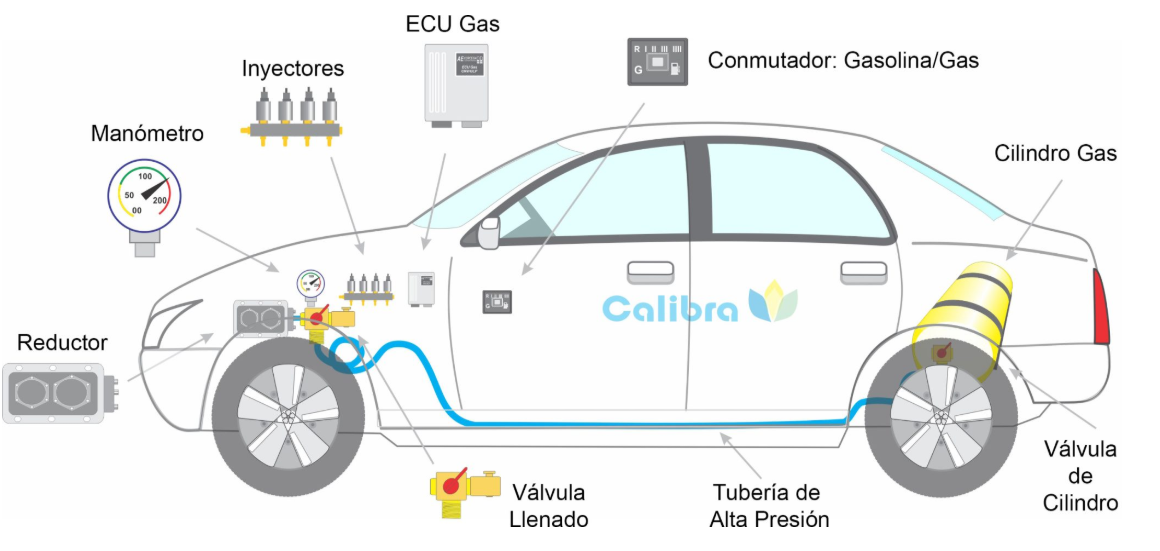
\includegraphics[width=0.95\textwidth]{Images/GLP.png}
	\vspace{0.2cm}
	
	% 3. La nota de la figura según APA 7 (Con descripción técnica)
	\begin{flushleft}
		\footnotesize \textit{Nota.} Arquitectura de instalación y flujo de señales en un motor adaptado para doble combustible, detallando la integración de la ECU secundaria de gas, el regulador de presión, la rampa de inyectores de GLP y el tanque de almacenamiento con su respectiva multivalvula. Adaptado de~\citep{GasNaturalGNU}.
	\end{flushleft}
\end{figure}

La elección del combustible alternativo depende de factores como la infraestructura disponible, el costo por unidad de energía, la autonomía requerida y la compatibilidad del sistema de inyección y encendido con las características del combustible \citep{GasNaturalGNU, BifuelMotor1}.

\subsection{Ventajas y desventajas}

Entre las principales ventajas de los vehículos bi-fuel se encuentra la posibilidad de extender la autonomía del vehículo al disponer de dos sistemas de alimentación, así como la reducción del costo operativo cuando se utiliza el combustible alternativo. Además, el uso de GLP o GNV suele asociarse con menores emisiones de CO$_2$ y NO$_x$, lo cual representa una ventaja ambiental frente al uso exclusivo de gasolina \citep{ GasNaturalGNU, Fedebiocombustibles}.

No obstante, este tipo de tecnología también presenta desventajas. En algunos casos, el motor puede experimentar una ligera reducción de potencia cuando opera con el combustible alternativo, especialmente en configuraciones a GLP. Asimismo, la instalación del sistema bi-fuel implica una mayor complejidad mecánica, costos iniciales más elevados y la necesidad de mantenimiento especializado \citep{ BifuelMotorES}.

\subsection{Impacto en el consumo de combustible}

El impacto de los vehículos bi-fuel sobre el consumo de combustible debe analizarse considerando que cada combustible posee una densidad energética distinta. En general, el consumo volumétrico con GLP o GNV puede ser mayor que con gasolina, aunque el costo por kilómetro recorrido puede disminuir debido al menor precio del combustible alternativo \citep{DRBifuel}.

En la práctica, la comparación del consumo debe realizarse en términos equivalentes de energía o costo operativo, ya que un mayor volumen consumido no necesariamente implica un mayor gasto económico. Por esta razón, los vehículos bi-fuel constituyen una alternativa interesante para aplicaciones donde se busca reducir el costo de operación y las emisiones, manteniendo la posibilidad de usar gasolina como respaldo energético \citep{GasNaturalGNU, BifuelMotorES}.

La Figura \ref{fig:bifuel_sistema2} puede utilizarse para mostrar la arquitectura general de un sistema bi-fuel, incluyendo los componentes principales del circuito de gasolina y del circuito de gas. Y seguidamente en la Tabla \ref{tab:bifuel} su comparación con diferentes combustibles.

\begin{figure}[h]
	\centering
	
	% 1. El caption automático estilo APA 7 (Título descriptivo arriba)
	\caption{Esquema de componentes que conforman un vehículo bi-fuel, mostrando la coexistencia de sistemas de inyección paralelos y su gestión electrónica integrada}
	\label{fig:bifuel_sistema2}
	\vspace{0.3cm}
	
	% 2. La imagen ajustada proporcionalmente para mantener simetría visual
	% Nota: Se redujo levemente a 0.95\textwidth para evitar desbordes accidentales
	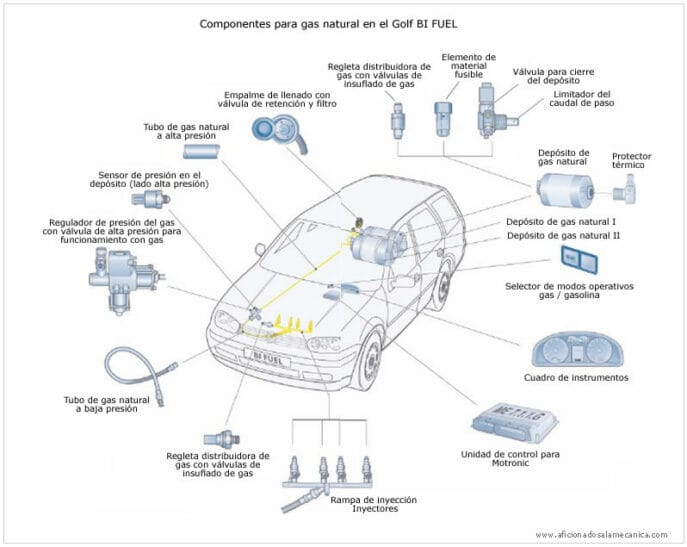
\includegraphics[width=0.95\textwidth]{Images/esquema-inyeccion-golf.jpg}
	\vspace{0.2cm}
	
	% 3. La nota de la figura según APA 7 (Con descripción técnica)
	\begin{flushleft}
		\footnotesize \textit{Nota.} Diagrama de bloques que ilustra la arquitectura de un motor adaptado para doble combustible (Gasolina/Gas). Se detalla la integración de la ECU secundaria, el regulador de presión, la rampa de inyectores de gas y el tanque de almacenamiento con su multivalvula, operando en paralelo al sistema de inyección original. Elaboración propia con base en~\citep{BifuelMotorES}.
	\end{flushleft}
\end{figure}

\begin{table}[h]
	\centering
	% Título separado bajo norma estricta APA 7
	\captionsetup{labelformat=simple, labelsep=newline, textfont=it, labelfont=bf}
	\caption{Comparación general entre combustibles en vehículos bi-fuel}
	\label{tab:bifuel}
	\vspace{0.3cm}
	
	% Usamos tabularx para una distribución fluida y adaptativa entre los márgenes
	\begin{tabularx}{\linewidth}{p{2.8cm} X X X}
		\toprule % Línea superior APA 7
		\rowcolor[rgb]{0.851, 0.851, 0.851}
		\textbf{Combustible} & \textbf{Ventaja principal} & \textbf{Limitación principal} & \textbf{Uso típico} \\
		\midrule % Línea divisoria de encabezado APA 7
		Gasolina & Mayor disponibilidad y arranque confiable en frío. & Mayor costo operativo y mayores emisiones de CO. & Operación principal o combustible de respaldo. \\
		\addlinespace
		GLP & Menor costo por kilómetro y reducción de emisiones. & Ligera pérdida de potencia y mayor consumo volumétrico. & Uso alternativo en vehículos convencionales adaptados. \\
		\addlinespace
		GNV & Alto rendimiento energético y bajas emisiones contaminantes. & Infraestructura de carga limitada y peso del tanque de almacenamiento. & Transporte urbano, flotas comerciales y transporte pesado. \\
		\bottomrule % Línea inferior de cierre APA 7
	\end{tabularx}
	\vspace{0.2cm}
	
	\begin{flushleft}
		\footnotesize \textit{Nota.} Comparación de parámetros operativos, económicos y logísticos de los combustibles más utilizados en vehículos dotados con sistemas de conversión de doble combustible. Elaboración propia.
	\end{flushleft}
\end{table}


%-------------------------2.9----------------
\section{Microcontroladores y sistemas embebidos}


\subsection{Microprocesador vs microcontrolador}
Un \textit{microprocesador} es un circuito integrado que contiene únicamente la unidad central de procesamiento (CPU), encargada de ejecutar instrucciones y procesar datos. Su función principal consiste en interpretar operaciones almacenadas en memoria externa, realizar cálculos aritméticos y lógicos y coordinar la ejecución de un programa mediante señales de control y buses de datos, direcciones e instrucciones .

A diferencia de otros dispositivos, el microprocesador por sí solo no forma un sistema funcional completo, ya que requiere memoria externa (RAM, ROM/Flash), periféricos de entrada/salida y circuitos auxiliares para operar en una aplicación real. Por esta razón, suele emplearse en sistemas de propósito general o en plataformas que demandan mayor capacidad de cómputo y flexibilidad, como computadoras de escritorio o sistemas de infoentretenimiento de alto nivel \citep{ MikroE2018}.

En contraste, un \textit{microcontrolador} integra en un solo chip la CPU, memoria (programa y datos) y periféricos de entrada y salida necesarios para ejecutar tareas específicas. Esta integración permite construir sistemas compactos, de bajo consumo y bajo costo, orientados a aplicación de control en tiempo real, como la gestión de sensores, actuadores y buses de comunicación. En el ámbito automotriz, los microcontroladores son ampliamente utilizados en unidades de control electrónico (ECU) para funciones de powertrain, chasis, seguridad y confort \citep{ EmbebidosUruguay}.

\subsection{Sistema embebido}
Un \textit{sistema embebido} es un sistema de cómputo diseñado para realizar una función específica dentro de un dispositivo o equipo mayor, en lugar de servir como plataforma de propósito general. Está compuesto por hardware (microcontrolador o microprocesador, sensores, actuadores, conversiones de señal, etc.), software (firmware o RTOS) y, en algunos casos, elementos mecánicos, con restricciones propias de tiempo, consumo energético y recursos disponibles \citep{EmbebidosUruguay, ITESOEmbebidos}.

Estos sistemas interactúan con el entorno físico mediante sensores y actuadores, y suelen operar en tiempo real o con tiempos de respuesta acotados. Debido a su naturaleza específica, se optimizan para resolver una tarea concreta (por ejemplo, medir el flujo de combustible, controlar el encendido o gestionar una bomba eléctrica) con alta confiabilidad, bajo costo y consumo reducido de energía. En la industria automotriz, prácticamente todas las ECUs presentes en el vehículo constituyen sistemas embebidos \citep{EmbebidosUruguay, AutomotiveEmbeddedHandbook}.

\subsection{Arquitectura de microcontroladores}

Como se ha señalado, un \textit{microcontrolador} combina núcleo, memoria RAM y periféricos. Con el fin de profundizar en su funcionamiento, en esta sección se describirán teóricamente estos elementos y se analizarán las arquitecturas que definen su estructura.

\subsubsection{Núcleo/CPU}
El núcleo o CPU de un microcontrolador es el bloque encargado de ejecutar las instrucciones del programa, gestionar registros internos y controlar el flujo de datos entre los distintos componentes del sistema. En la actualidad, los microcontroladores más utilizados en aplicaciones automotrices se basan en arquitecturas de tipo RISC, como los núcleos ARM Cortex‑M, AVR o PIC , que ofrecen un buen equilibrio entre rendimiento, consumo energético y facilidad de programación \citep{MikroE2018}.

Estos últimos se detallan en la Tabla \ref{tab:arqui}

\begin{table}[htbp]
	\centering
	% Título separado bajo norma estricta APA 7
	\captionsetup{labelformat=simple, labelsep=newline, textfont=it, labelfont=bf}
	\caption{Comparación de arquitecturas de CPU en sistemas embebidos y computación}
	\label{tab:arqui}
	\vspace{0.3cm}
	
	% Usamos tabularx para un autoajuste exacto a los márgenes del documento
	\begin{tabularx}{\linewidth}{p{2.2cm} X X X p{2.8cm}}
		\toprule % Línea superior APA 7
		\rowcolor[rgb]{0.851, 0.851, 0.851}
		\textbf{Arquitectura} & \textbf{Principio clave} & \textbf{Ventaja principal} & \textbf{Desventaja principal} & \textbf{Ejemplos} \\
		\midrule % Línea divisoria de encabezado APA 7
		\textbf{Harvard} & Buses físicos separados para datos e instrucciones. Permite accesos simultáneos. & Mayor velocidad de procesamiento y paralelismo básico. & Hardware más complejo de diseñar y cablear. & PIC, AVR (Arduino), ARM Cortex-M (ESP32, Pi Pico). \\
		\addlinespace
		\textbf{Von Neumann} & Un solo bus compartido para datos e instrucciones. Acceso de tipo secuencial. & Estructura más simple y mapa de memoria continuo. & Cuello de botella en el bus (ralentiza el sistema). & MSP430, Intel 8051 clásico, arquitectura de PC. \\
		\addlinespace
		\textbf{RISC} & Juego de instrucciones simples y de tamaño fijo. Ejecución en un ciclo de reloj. & Ejecución rápida, eficiente y con bajo consumo energético. & Requiere mayor cantidad de líneas de código compilado. & AVR, ARM Cortex-M, PIC modernos, RISC-V. \\
		\addlinespace
		\textbf{CISC} & Instrucciones complejas y de longitud variable para tareas múltiples. & Código binario más compacto (optimiza el uso de memoria). & Mayor consumo de potencia y tiempos de ejecución variables. & Procesadores de PC comerciales (x86), familias Renesas. \\
		\bottomrule % Línea inferior de cierre APA 7
	\end{tabularx}
	\vspace{0.2cm}
	
	\begin{flushleft}
		\footnotesize \textit{Nota.} Comparación estructural de los criterios de diseño de hardware para el procesamiento de datos en microcontroladores y procesadores modernos. Elaboración propia.
	\end{flushleft}
\end{table}


Dentro de la CPU se encuentran la unidad de control, que coordina el ciclo de instrucción, y la unidad aritmético‑lógica (ALU), que realiza operaciones aritméticas y lógicas sobre los datos. Los registros internos almacenan temporalmente direcciones, datos de trabajo e información de estado (flag de condición), lo que permite una ejecución rápida sin necesidad de acceder continuamente a la memoria principal.

\subsubsection{Memoria on‑chip}
Los microcontroladores integran en el mismo chip varios tipos de memoria, cada uno orientado a una función específica. La memoria de programa, típicamente Flash o ROM, almacena el código ejecutable del firmware, permitiendo leer e, idealmente, reprogramar el dispositivo en campo. La memoria de datos (SRAM) guarda variables temporales, pilas de ejecución y estructuras de datos mientras el sistema está activo, aunque su contenido se pierde al desconectar la alimentación, mas detalle acerca de estas memorias en la Tabla \ref{tab:memo}.

\begin{table}[h]
	\centering
	% Título separado bajo norma estricta APA 7
	\captionsetup{labelformat=simple, labelsep=newline, textfont=it, labelfont=bf}
	\caption{Clasificación y funciones de las memorias en un microcontrolador}
	\label{tab:memo}
	\vspace{0.3cm}
	
	% Usamos tabularx para un autoajuste exacto a los márgenes del documento
	\begin{tabularx}{\linewidth}{p{3.2cm} p{2.2cm} X p{2.8cm}}
		\toprule % Línea superior APA 7
		\rowcolor[rgb]{0.851, 0.851, 0.851}
		\textbf{Tipo de memoria} & \textbf{Volatilidad} & \textbf{Función principal} & \textbf{Velocidad} \\
		\midrule % Línea divisoria de encabezado APA 7
		\textbf{Flash} & No volátil & Almacenar el código del programa fuente (firmware) y constantes del sistema. & Alta / Media. \\
		\addlinespace
		\textbf{RAM (SRAM)} & Volátil & Almacenar variables temporales, pilas de ejecución y datos de sensores en tiempo real. & Muy Alta. \\
		\addlinespace
		\textbf{EEPROM} & No volátil & Almacenar parámetros de calibración y datos de configuración del usuario que deben persistir. & Baja. \\
		\addlinespace
		\textbf{Registros} & Volátil & Espacio de trabajo directo del núcleo de la CPU para operaciones aritmético-lógicas. & Máxima (Inmediata). \\
		\addlinespace
		\textbf{ROM / Bootloader} & No volátil & Almacenar el código de arranque y rutinas de fábrica inalterables para la programación del chip. & Alta. \\
		\bottomrule % Línea inferior de cierre APA 7
	\end{tabularx}
	\vspace{0.2cm}
	
	\begin{flushleft}
		\footnotesize \textit{Nota.} Organización jerárquica y segmentación funcional del mapa de memoria interno característico en arquitecturas de sistemas embebidos modernos. Elaboración propia.
	\end{flushleft}
\end{table}

En muchos microcontroladores automotrices se incluye también memoria EEPROM o una sección de Flash configurada como memoria no volátil, utilizada para almacenar parámetros de calibración, configuraciones de usuario o datos de diagnóstico que deben preservarse entre encendidos. La coexistencia de Flash, SRAM y, en algunos casos, EEPROM permite una arquitectura de memoria eficiente y adecuada para aplicaciones de control críticas.

\subsubsection{Periféricos integrados}
Los periféricos integrados son módulos especializados que permiten al microcontrolador interactuar con el mundo externo de forma directa. Entre los más comunes se encuentran los convertidores analógico‑digital (ADC), que permiten leer señales de sensores como presión, temperatura o voltaje; los convertidores digital‑analógico (DAC), que generan señales continuas para controlar actuadores lineales; y los timers o temporizadores, que permiten la medición de tiempos, la generación de señales PWM o la implementación de rutinas periódicas \citep{EmbebidosUruguay, AutomotiveEmbeddedHandbook}.

Además, los microcontroladores incluyen módulos de comunicación serie como UART, SPI e I2C, que permiten la comunicación con dispositivos externos (sensores, displays, módulos de radio, etc.) con bajo costo y alta integración. Otros periféricos típicos incluyen GPIO (pines de entrada/salida digitales configurables), comparadores analógicos, watchdog timers y módulos de captura/comparación, todos diseñados para simplificar el control de señales en tiempo real.

\subsubsection{Controladores de comunicación}
En el ámbito automotriz, los microcontroladores suelen integrar controladores de comunicación especializados para buses como CAN, LIN y, en algunos casos, FlexRay o Automotive Ethernet. El controlador CAN, por ejemplo, gestiona la trama CAN conforme a la norma ISO 11898, permitiendo la transmisión y recepción de mensajes sin que el núcleo tenga que gestionar cada bit, lo que alivia la carga de procesamiento y mejora la determinismo en la comunicación de datos entre ECUs \citep{ISO11898, AutomotiveEmbeddedHandbook}.

Los módulos LIN permiten la creación de redes de bajo costo para subsistemas de confort y body electronics, mientras que módulos de Ethernet o FlexRay se utilizan en aplicaciones de mayor ancho de banda o requisitos de tiempo real estrictos, como sistemas de infoentretenimiento o ADAS. La presencia de estos controladores de comunicación integrados convierte al microcontrolador en un nodo de red listo para integrarse en la arquitectura de comunicación vehicular sin necesidad de circuitos externos complejos.

\subsubsection{Subsistemas de energía y gestión}
Los microcontroladores incluyen subsistemas de energía y gestión que permiten operar en entornos de alto consumo dinámico y garantizar la confiabilidad del sistema. Entre estos se encuentran módulos de regulación de voltaje interna, circuitos de brown‑out detection (que detectan caídas de tensión peligrosas), osciladores de reloj internos y externos, y módulos de bajo consumo que permiten activar distintos modos de ahorro de energía (sleep, standby, power‑down) según el estado de la aplicación \citep{MikroE2018}.

El watchdog timer (WDT) es un módulo fundamental en sistemas críticos, ya que reinicia el microcontrolador si el software deja de ejecutar periódicamente una rutina de “alimentación” del temporizador, corrigiendo así bloqueos o estados indecisos del firmware. Estos mecanismos combinados (modos de bajo consumo, brown‑out detection, WDT y supervisión de reloj) son esenciales en aplicaciones automotrices, donde la falencia de un sistema de control puede tener consecuencias de seguridad y operativas significativas.

En la Figura \ref{fig:MICRO_R} se presenta un esquema genérico de la arquitectura de un \textit{microcontrolador}

\begin{figure}[h]
	\centering
	
	% 1. El caption automático estilo APA 7 (Título descriptivo arriba)
	\caption{Diagrama de bloques general de la arquitectura interna de un microcontrolador estándar}
	\label{fig:MICRO_R}
	\vspace{0.3cm}
	
	% 2. La imagen ajustada proporcionalmente para mantener simetría visual
	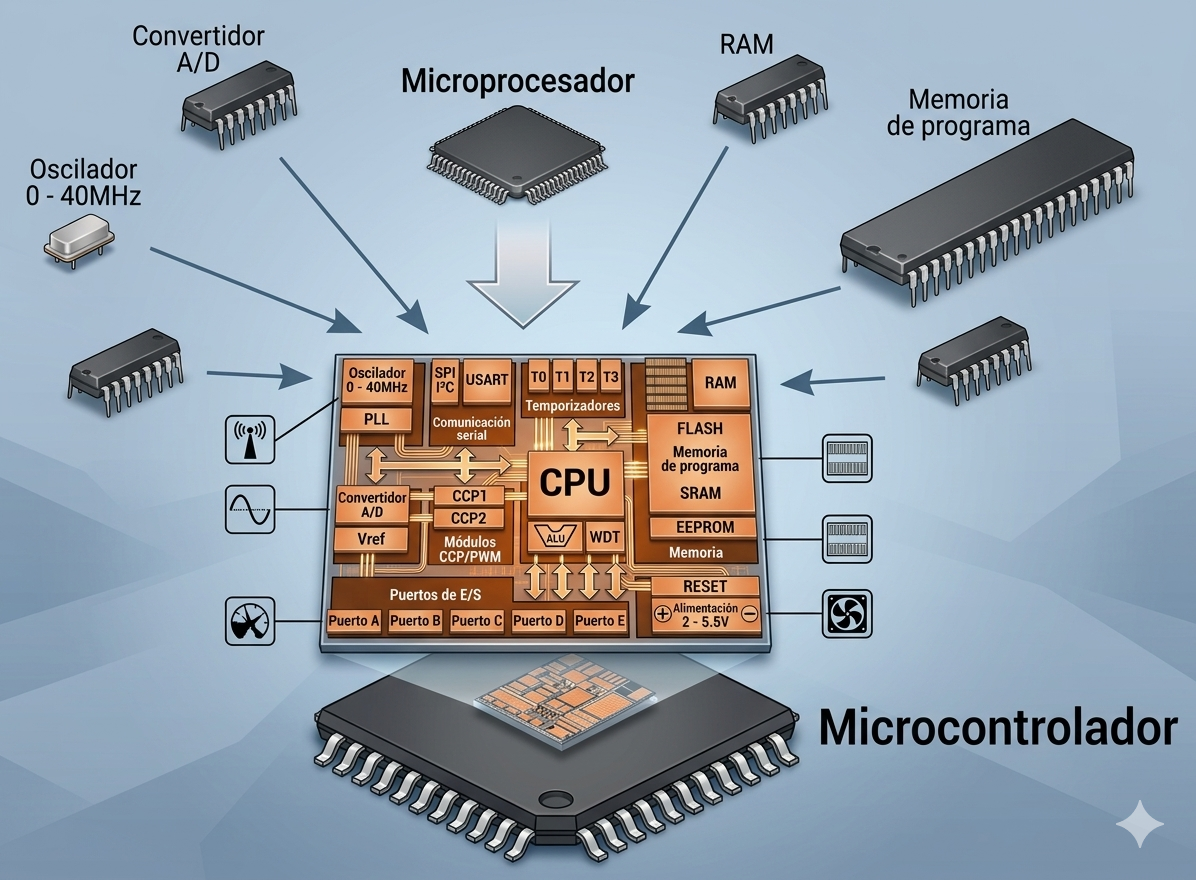
\includegraphics[width=0.75\textwidth]{Images/MICRO_E.png}
	\vspace{0.2cm}
	
	% 3. La nota de la figura según APA 7 (Con descripción técnica)
	\begin{flushleft}
		\footnotesize \textit{Nota.} Interconectividad de los componentes modulares del dispositivo, ilustrando el núcleo de procesamiento (CPU), las unidades de memoria volátil y no volátil, las líneas de los buses internos y la distribución de los periféricos de entrada y salida (I/O). Adaptado de~\citep{aprendiendoarduino2016}.
	\end{flushleft}
\end{figure}


\subsection{Programación y desarrollo de firmware}
\subsubsection{Lenguajes y paradigmas de programación}
El desarrollo de firmware para microcontroladores se realiza principalmente en lenguajes de bajo nivel pero de alto rendimiento, destacando el uso de \textit{C} y, en menor medida, \textit{C++}. Estos lenguajes permiten un control fino sobre el hardware, manejo directo de registros y periféricos, y optimización de memoria y tiempo de ejecución, aspectos críticos en sistemas embebidos de recursos limitados \citep{EmbebidosUruguay}.

En secciones críticas, como manejo de interrupciones o rutinas de tiempo real extremadamente acotado, se emplea también \textit{ensamblador} para reducir la latencia y aprovechar al máximo las características del núcleo. Además, se utilizan paradigmas de programación orientados a eventos y a tareas, mediante el uso de rutinas de servicio de interrupción (ISR), bucles principales con polling y, cuando se emplea un RTOS, ejecución de tareas concurrentes con prioridades bien definidas .

\subsubsection{Software bare‑metal y RTOS}
El \textit{bare‑metal programming} se refiere al desarrollo de firmware sin sistema operativo, donde el programador gestiona directamente el hardware, los registros y el flujo de ejecución. Este enfoque minimiza el uso de memoria y la latencia de respuesta, resultando adecuado para sistemas relativamente simples o de máxima crítica en tiempo real, como ciertas ECUs de sensado y control básico \citep{EmbebidosUruguay}.

Cuando la complejidad del sistema crece (múltiples tareas, comunicación asincrónica, gestión de recursos compartidos), se recurre a \textit{sistemas operativos en tiempo real} (RTOS) como FreeRTOS, que permiten ejecutar tareas concurrentes, gestionar colas de mensajes, semáforos y prioridades de forma determinista. Los RTOS son ampliamente utilizados en ECUs automotrices donde se requiere coordinar diversas funcionalidades (lectura de sensores, control de actuadores, comunicación CAN) con tiempos de respuesta garantizados \citep{AutomotiveEmbeddedHandbook}.

\subsubsection{Herramientas de desarrollo y depuración}
El desarrollo de firmware se apoya en una cadena de herramientas conocida como \textit{toolchain}, compuesta por compiladores (por ejemplo, GCC para ARM o herramientas del fabricante), ensambladores, enlazadores y librerías de bajo nivel. Estas herramientas transforman el código fuente en un binario que se graba en la memoria del microcontrolador y se ejecuta en el sistema objetivo .

La depuración se realiza mediante interfaces como JTAG o SWD, que permiten detener la ejecución, inspeccionar variables, modificar el flujo de control y monitorear señales de control en tiempo real. Entornos de desarrollo integrados (IDE) y simuladores ayudan a realizar pruebas tempranas y a validar algoritmos sin necesidad de hardware físico, aumentando la productividad y reduciendo errores en el diseño de firmware \citep{EmbebidosUruguay}.

\subsubsection{Pruebas y validación de firmware}
La validación de firmware incluye pruebas unitarias, pruebas de integración y, en sistemas críticos, pruebas en configuración hardware in the loop (HIL), donde la ECU se conecta a un simulador de vehículo que replica el comportamiento de sensores y actuadores. Estas pruebas permiten verificar el cumplimiento de requisitos de funcionalidad, seguridad y tiempo real antes de la puesta en marcha en el vehículo real \citep{AutomotiveEmbeddedHandbook}.

Además, se emplean técnicas de análisis estático de código, inspección de cubrimiento de pruebas y auditorías de seguridad funcional para detectar errores tempranos y asegurar que el firmware cumpla con normas de calidad y estándares de la industria automotriz.

\subsection{Comunicación y redes embebidas en automoción}
\subsubsection{CAN / CAN‑FD}
El bus \textit{CAN} (Controller Area Network), definido por la norma ISO 11898, es el estándar de comunicación más extendido en vehículos modernos. Permite interconectar múltiples unidades de control electrónico (ECU) mediante un par trenzado y protocolo de comunicación de mensajes orientado a datos, con alta inmunidad al ruido y mecanismos de arbitraje basados en la prioridad de la identificación de mensaje \citep{AutomotiveEmbeddedHandbook}.

CAN‑FD (CAN with Flexible Data Rate) es una evolución que mantiene compatibilidad con CAN clásico, pero permite velocidades de línea y tamaños de payload mayores, lo que mejora el ancho de banda disponible para datos de diagnóstico, sensores de alto volumen y sistemas ADAS. En sistemas embebidos automotrices, el uso de CAN/CAN‑FD es fundamental para la coordinación de ECUs de motor, transmisión, chasis y seguridad de forma robusta y determinista.

\subsubsection{LIN, FlexRay y Automotive Ethernet}
El bus \textit{LIN} (Local Interconnect Network) se utiliza para redes de bajo costo y baja velocidad, orientadas a subsistemas de confort y body electronics, como ventanas, cerraduras, sensores de puerta y luces interiores. LIN funciona sobre un solo cable y emplea una arquitectura maestro‑esclavo, lo que lo hace adecuado para aplicaciones no críticas en tiempo real pero sensibles al costo \citep{ AutomotiveEmbeddedHandbook}.

\textit{FlexRay} ofrece un bus de alta velocidad y alta fiabilidad, orientado a sistemas de tiempo real estricto como control de estabilidad, suspensión activa y algunas arquitecturas de seguridad. Proporciona latencias predecibles y tolerancia a fallos, pero con un costo de hardware y desarrollo más elevado respecto a CAN. En paralelo, \textit{Automotive Ethernet} aparece como solución para sistemas de alto ancho de banda, como infoentretenimiento, telemetría avanzada y comunicaciones entre dominios mediante redes IP dentro del vehículo.

\subsubsection{Protocolos de diagnóstico (OBD‑II, UDS)}
La normativa internacional de diagnósticos vehiculares se basa principalmente en el \textit{OBD‑II} (On‑Board Diagnostics II), que define formatos de conectores, mensajes básicos y códigos de fallo genéricos accesibles mediante lectores comerciales. Este protocolo permite la lectura remota de códigos DTC, el monitoreo de parámetros de funcionamiento y el borrado de fallos, facilitando el mantenimiento y la verificación emisiones \citep{ AutomotiveEmbeddedHandbook}.

Por encima de la capa física y de transporte se encuentra el protocolo \textit{UDS} (Unified Diagnostic Services, ISO 14229), que define servicios estandarizados como lectura y escritura de datos de diagnóstico, arranque de rutinas, acceso a memoria y reprogramación de firmware vía CAN (ISO 15765). 

\subsection{Requisitos eléctricos y ambientales}
\subsubsection{Rangos de tensión y transientes}

Los microcontroladores empleados en entornos automotrices deben operar de forma confiable dentro de un sistema eléctrico cuya tensión nominal es de 12\,V en vehículos de combustión interna convencionales, 24\,V en vehículos comerciales y camiones pesados, y 48\,V en arquitecturas de red de a bordo híbridas de tipo \textit{mild-hybrid} \citep{Zimmermann2014}.

La norma \textbf{ISO~16750-2} \citep{ISO16750} establece los perfiles de tensión que todo componente electrónico automotriz debe tolerar, clasificándolos en condiciones de operación normal, condiciones límite y eventos transitorios. En condiciones normales, la tensión de batería de un sistema de 12\,V oscila entre 9\,V y 16\,V durante la operación del alternador.

Los principales fenómenos transitorios reconocidos por \textbf{ISO~7637-2} 
\citep{ISO7637} e \textbf{ISO~16750-2} se describen a continuación:

\begin{itemize}
	\item \textbf{Pulso 1 — Load Dump:} Ocurre cuando la batería se desconecta 
	abruptamente mientras el alternador está en plena carga. Genera pulsos de 
	tensión que pueden superar los $+100$\,V con una duración de hasta 400\,ms. 
	Es el transitorio de mayor energía y requiere supresores de tensión tipo TVS 
	(\textit{Transient Voltage Suppressor}) o varistores de óxido metálico (MOV) 
	en la etapa de entrada de alimentación \citep{Tarter1991}.
	
	\item \textbf{Pulso 2a/2b — Interrupción inductiva:} Producido por la apertura 
	de cargas inductivas (relés, solenoides). Genera pulsos negativos de hasta 
	$-100$\,V y pulsos positivos de corta duración en el bus.
	
	\item \textbf{Pulso 3a/3b — Switching transients:} Originados por la 
	conmutación de cargas en el mismo bus. Presentan amplitudes de $\pm100$\,V 
	con duraciones del orden de los microsegundos y alta repetitividad.
	
	\item \textbf{Pulso 4 — Arranque del motor:} Durante el encendido, el motor 
	de arranque produce una caída de tensión que puede llevar el bus de 12\,V 
	hasta valores de 4--6\,V por intervalos de hasta 150\,ms. Los 
	microcontroladores deben mantener su estado operativo o ejecutar un 
	\textit{reset} controlado en este escenario \citep{Bosch2014}.
	
	\item \textbf{Pulso 5a/5b — Jump start / sobretensión de carga:} Un arranque 
	con cables de puente puede elevar la tensión hasta 24\,V en un sistema de 
	12\,V. Los reguladores de tensión de la ECU deben absorber esta condición 
	sin degradarse.
\end{itemize}

La Figura~\ref{fig:transitorios_automotriz} ilustra de forma esquemática la 
morfología temporal de los pulsos más representativos sobre un bus de 12\,V.

\begin{figure}[h]
	\centering
	
	% 1. El caption automático estilo APA 7 (Título descriptivo arriba)
	\caption{Perfiles morfológicos de los principales transitorios de tensión en un sistema eléctrico automotriz de 12\,V}
	\label{fig:transitorios_automotriz}
	\vspace{0.3cm}
	
	% 2. La imagen ajustada proporcionalmente para mantener simetría visual
	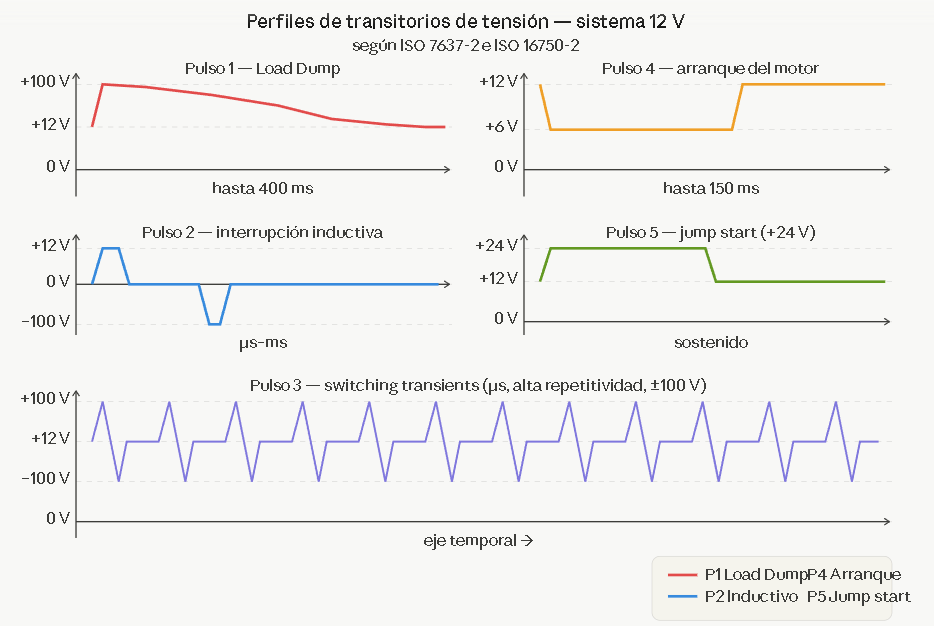
\includegraphics[width=0.95\textwidth]{Images/transitorios_automotriz.png}
	\vspace{0.2cm}
	
	% 3. La nota de la figura según APA 7 (Con la descripción y normas técnicas completas)
	\begin{flushleft}
		\footnotesize \textit{Nota.} Comportamiento temporal y formas de onda de los pulsos de voltaje críticos conforme a las normativas ISO~7637-2 e ISO~16750-2. Los pulsos 1 y 5 representan las condiciones de mayor descarga de energía (como el fenómeno de \textit{Load Dump}), mientras que el pulso 3 detalla las ráfagas de alta frecuencia provocadas por conmutaciones de relés y acoplamientos capacitivos. Elaboración propia.
	\end{flushleft}
\end{figure}

Para garantizar la integridad de las ECU frente a estos eventos, los diseñadores 
recurren a una cadena de protección en la etapa de entrada de alimentación que 
combina varios dispositivos \citep{Bosch2014}:

\begin{enumerate}
	\item \textbf{Fusible o PTC:} Primera barrera contra sobrecorriente sostenida.
	
	\item \textbf{MOV / TVS bidireccional:} Absorbe la energía del Load Dump y 
	los pulsos positivos de alta tensión. Los diodos TVS (p.\,ej., serie SMBJ) 
	ofrecen tiempos de respuesta del orden de los picosegundos.
	
	\item \textbf{Inductor de modo común y condensador de desacoplo:} Filtra los 
	transitorios de alta frecuencia (pulso~3) y desacopla el bus de la 
	electrónica interna.
	
	\item \textbf{Regulador de tensión (LDO o SMPS):} Provee la tensión 
	estabilizada de 5\,V o 3{,}3\,V al MCU, con rechazo de rizado (PSRR) y 
	protección de subvoltaje (\textit{undervoltage lockout}, UVLO) para gestionar 
	correctamente la caída producida durante el arranque (pulso~4).
	
	\item \textbf{Supervisor de tensión:} Circuito dedicado (p.\,ej., TPS3840) 
	que monitoriza continuamente la alimentación y genera un \textit{reset} 
	controlado ante condiciones fuera de rango, garantizando la integridad del 
	firmware almacenado en memoria no volátil.
\end{enumerate}

Los microcontroladores automotrices modernos, como el Renesas RH850 o el 
NXP~S32K3, incorporan internamente circuitos de UVLO y detectores de 
\textit{brown-out} conformes con los requisitos de ISO~16750-2, reduciendo la 
cantidad de componentes externos necesarios en el diseño de la ECU 
\citep{Renesas2021, NXP2022}.


%%%─────────────────────────────────────────────────────────────
\subsection{Aplicaciones en la industria automotriz}

Los microcontroladores (MCU) constituyen el núcleo computacional de las
unidades de control electrónico (\textit{Electronic Control Unit}, ECU) que
gobiernan la práctica totalidad de los subsistemas de un vehículo moderno.
Según estimaciones de la industria, un automóvil de gama media-alta incorpora
entre 70 y 100 ECUs independientes, cifra que en vehículos premium o eléctricos
puede superar las 150 unidades \citep{Bosch2014}. Estas ECUs se agrupan
funcionalmente en dominios que comparten buses de comunicación, requisitos de
integridad y restricciones de tiempo real, tal como se ilustra en la
Figura~\ref{fig:dominios_ecu}.

\begin{figure}[h]
	\centering
	
	% 1. El caption automático estilo APA 7 (Título descriptivo conciso arriba)
	\caption{Arquitectura y distribución de dominios de ECUs en un vehículo moderno}
	\label{fig:dominios_ecu}
	\vspace{0.3cm}
	
	% 2. La imagen ajustada proporcionalmente para mantener simetría visual
	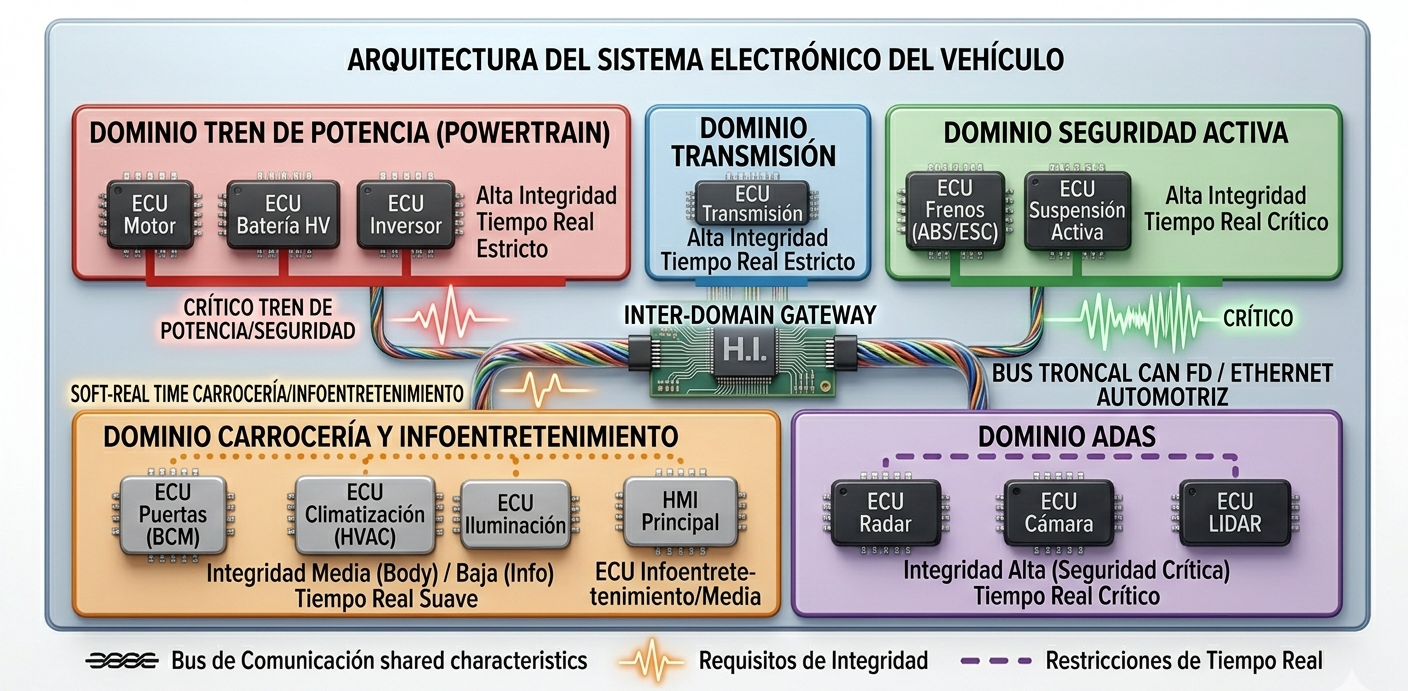
\includegraphics[width=0.95\textwidth]{Images/dominios_ecu.png}
	\vspace{0.2cm}
	
	% 3. La nota de la figura según APA 7 (Con la descripción técnica detallada)
	\begin{flushleft}
		\footnotesize \textit{Nota.} Organización funcional del sistema electrónico del vehículo dividida en cinco dominios principales: \textit{powertrain}, transmisión, seguridad activa, \textit{body}/infoentretenimiento y sistemas avanzados de asistencia al conductor (ADAS). Se ilustra la interconectividad y el flujo de datos masivo a través de un bus troncal central basado en las tecnologías CAN\,FD y Ethernet automotriz. Elaboración propia.
	\end{flushleft}
\end{figure}

%%%─────────────────────────────────────────────────────────────
\subsection{ECUs de powertrain}

El dominio de \textit{powertrain} agrupa las ECUs responsables de la gestión
energética del tren de potencia, siendo la más relevante la unidad de control
del motor (\textit{Engine Management System}, EMS o ECM). Su función principal
consiste en optimizar los procesos de dosificación de combustible, encendido y
control de emisiones, garantizando simultáneamente el rendimiento dinámico
exigido por el conductor y el cumplimiento de las normativas de emisiones
EURO\,6d y EPA Tier\,3 \citep{Reif2015}.

\subsubsection{Funciones principales de la ECM}

La ECM adquiere señales de un conjunto de sensores —cigüeñal, árbol de levas,
masa de aire (MAF), presión absoluta en colector (MAP), sonda lambda de banda
ancha, temperatura de refrigerante y presión de combustible— y ejecuta, en
tiempo real, los algoritmos de:

\begin{itemize}
	\item \textbf{Cálculo de tiempo de inyección (\textit{injection pulse width},
		IPW):} basado en modelos de carga volumétrica y correcciones adaptativas
	por desvíos lambda \citep{Bosch2014}.
	\item \textbf{Avance de encendido:} optimizado ciclo a ciclo mediante el
	detector de detonación (\textit{knock sensor}); en motores modernos
	con encendido por compresión (HCCI), el control se realiza
	por temperatura en cámara \citep{Heywood2018}.
	\item \textbf{Gestión del par:} coordinación con la TCU y con el sistema
	ESP para garantizar transferencia de par coherente en maniobras de
	cambio o corrección de estabilidad.
	\item \textbf{Control de emisiones:} regeneración del filtro de partículas
	(DPF), dosificación de AdBlue para reducción catalítica selectiva (SCR)
	y monitorización del sistema OBD-II conforme a ISO~15031 \citep{sae_j1979_2014}.
\end{itemize}

\subsubsection{Requerimientos computacionales}

La ECM opera con ciclos de control de hasta 1\,ms para las tareas de alta
prioridad (inyección, encendido) y ciclos de 10--100\,ms para las tareas de
diagnóstico y adaptación. Esto impone el uso de MCUs de 32\,bits con núcleos
duales en configuración \textit{lockstep} —como el Infineon AURIX TC3xx o el
NXP S32K3— capaces de ejecutar entre 200 y 800\,DMIPS con memorias Flash de
hasta 16\,MB y RAM de hasta 6\,MB \citep{Infineon2022, NXP2022} ver Tabla \ref{tab:mcu_ecm}.

\begin{table}[h]
	\centering
	% Título separado bajo norma estricta APA 7
	\captionsetup{labelformat=simple, labelsep=newline, textfont=it, labelfont=bf}
	\caption{Parámetros típicos de microcontroladores utilizados en módulos de control de motor de producción}
	\label{tab:mcu_ecm}
	
	% Ajuste de espaciado vertical de filas para una lectura cómoda
	\renewcommand{\arraystretch}{1.25}
	
	% Usamos tabularx con alineación centrada para las columnas cuantitativas
	\begin{tabularx}{\linewidth}{X c c c c c}
		\toprule % Línea superior APA 7
		\rowcolor[rgb]{0.851, 0.851, 0.851}
		\textbf{Familia} & \textbf{Núcleos} & \textbf{Frec. (MHz)} & \textbf{Flash (MB)} & \textbf{RAM (KB)} & \textbf{ASIL} \\
		\midrule % Línea divisoria de encabezado APA 7
		AURIX TC39x & 6 $\times$ TriCore & 300 & 16 & 6\,272 & D \\
		\addlinespace
		S32K396 & 4 $\times$ CM7 & 320 & 16 & 4\,096 & D \\
		\addlinespace
		RH850/U2A & 8 $\times$ G4MH & 400 & 16 & 7\,680 & D \\
		\addlinespace
		SPC58xEx & 4 $\times$ e200z7 & 200 & 8 & 1\,536 & D \\
		\bottomrule % Línea inferior de cierre APA 7
	\end{tabularx}
	\vspace{0.2cm}
	
	\begin{flushleft}
		\footnotesize \textit{Nota.} Criterios de rendimiento, almacenamiento y niveles de integridad de seguridad de la arquitectura automotriz (ASIL) en semiconductores integrados para la gestión del \textit{powertrain}. Elaboración propia.
	\end{flushleft}
\end{table}

La arquitectura \textit{lockstep} duplica la ejecución en dos núcleos idénticos
comparando los resultados en cada ciclo de reloj; cualquier discrepancia activa
un manejador de fallo seguro, lo que constituye un requisito indispensable
para alcanzar el nivel ASIL-D según ISO~26262 \citep{ISO16750}.

%%%─────────────────────────────────────────────────────────────
%\subsection{Control de transmisión (TCU)}
%
%La unidad de control de transmisión (\textit{Transmission Control Unit}, TCU)
%gestiona la lógica de cambio de marchas, la presión hidráulica de los embragues
%y la coordinación de par entre el motor y la caja de cambios \citep{Naunheimer2011}.
%En transmisiones automáticas de convertidor de par (AT), de doble embrague (DCT)
%y de variación continua (CVT), la TCU es la pieza central que determina el
%confort de cambio, la eficiencia energética y la protección mecánica del conjunto.
%
%\subsubsection{Estrategias de control}
%
%Las TCUs modernas implementan tres capas de control:
%
%\begin{enumerate}
%	\item \textbf{Capa de estrategia:} decide el punto de cambio óptimo a partir
%	de mapas multidimensionales que relacionan velocidad del vehículo, posición
%	del acelerador, pendiente de la calzada (estimada por el acelerómetro del
%	ESP) y modo de conducción seleccionado (Sport, Eco, Manual).
%	\item \textbf{Capa de control hidráulico:} regula solenoides de presión y
%	flujo con lazos PID de alta velocidad (ciclos de 1--5\,ms) para garantizar
%	el llenado y vaciado de los embragues dentro de las ventanas de tiempo de
%	cambio establecidas ($<$600\,ms en AT convencional,
%	$<$200\,ms en DCT) \citep{Naunheimer2011}.
%	\item \textbf{Capa de coordinación:} se comunica con la ECM vía CAN para
%	solicitar reducciones de par durante el cambio y evitar el impacto de
%	tracción (\textit{shift shock}).
%\end{enumerate}
%
%\subsubsection{Comunicación y diagnóstico}
%
%La TCU opera en el bus CAN\,HS a 500\,kbit/s e intercambia tramas con la ECM,
%el módulo ABS/ESP y la pantalla de instrumentos. A través del protocolo
%UDS (ISO~14229) expone parámetros de diagnóstico (temperatura de aceite,
%presión de embrague, número de cambios acumulados) accesibles con herramientas
%OBD-II de taller \citep{ISO14229} Algunas comparatuvas se presentan en la Tabla \ref{tab:tipos_tcu}.
%
%\begin{table}[h]
%	\centering
%	% Título separado bajo norma estricta APA 7
%	\captionsetup{labelformat=simple, labelsep=newline, textfont=it, labelfont=bf}
%	\caption{Comparativa de tipos de transmisión automática y requisitos de la unidad de control de transmisión}
%	\label{tab:tipos_tcu}
%	
%	% Ajuste de espaciado vertical de filas para mantener consistencia visual
%	\renewcommand{\arraystretch}{1.25}
%	
%	% Usamos tabularx con alineación centrada para las columnas de datos de ingeniería
%	\begin{tabularx}{\linewidth}{X c c c c}
%		\toprule % Línea superior APA 7
%		\rowcolor[rgb]{0.851, 0.851, 0.851}
%		\textbf{Tipo} & \textbf{Ciclo ctrl.} & \textbf{Solenoides} & \textbf{Bus CAN} & \textbf{ASIL} \\
%		\midrule % Línea divisoria de encabezado APA 7
%		AT conv. (6--10 vel.) & 5\,ms & 6--10 & HS 500 kbit/s & B \\
%		\addlinespace
%		DCT (7 vel.) & 1\,ms & 12--16 & HS 500 kbit/s & C \\
%		\addlinespace
%		CVT & 2\,ms & 4--6 & HS 500 kbit/s & B \\
%		\addlinespace
%		Híbrido P2 (DCT + motor) & 1\,ms & 16+ & CAN FD 2 Mbit/s & C \\
%		\bottomrule % Línea inferior de cierre APA 7
%	\end{tabularx}
%	\vspace{0.2cm}
%	
%	\begin{flushleft}
%		\footnotesize \textit{Nota.} Criterios de diseño temporal, demanda de actuadores hidráulicos, velocidad del bus de datos y requerimientos de seguridad funcional (ASIL) según la arquitectura de la transmisión. Elaboración propia.
%	\end{flushleft}
%\end{table}
%
%%%%─────────────────────────────────────────────────────────────
%\subsection{Sistemas de seguridad}
%
%Los sistemas de seguridad activa constituyen el dominio de mayor criticidad
%funcional del vehículo. Sus ECUs deben alcanzar el nivel ASIL-D —el más
%elevado de la norma ISO~26262— y garantizar la ejecución correcta de sus
%funciones incluso ante fallos de hardware o software \citep{ISO16750}.
%Este dominio comprende principalmente: el módulo de control de frenos
%(ABS/ESP/TCS), el actuador de dirección asistida eléctrica (EPS) y la unidad
%de control del airbag (ACU).
%
%\subsubsection{ABS / ESP / TCS}
%
%El sistema antibloqueo de frenos (ABS) y el programa electrónico de
%estabilidad (ESP) comparten una ECU que adquiere señales de velocidad en
%cada rueda (sensores de efecto Hall ABS), aceleración lateral e
%inercial (IMU de 6 ejes) y presión en el circuito de frenos. El algoritmo
%ESP detecta la divergencia entre la trayectoria deseada (calculada a partir
%del ángulo de volante y la velocidad del vehículo) y la real (medida con el
%giróscopo de guiñada), aplicando frenadas selectivas en las ruedas individua\-les
%con una resolución de par de 1\,Nm y tiempos de respuesta inferiores a
%20\,ms \citep{Bosch2014}.
%
%La ECU del ESP opera típicamente con un MCU de arquitectura \textit{lockstep}
%a 160--200\,MHz, conectado a dos módulos de accionamiento hidráulico mediante
%un bus privado de alta velocidad (FlexRay a 10\,Mbit/s o CAN\,FD a 5\,Mbit/s)
%para minimizar la latencia de actuación \citep{FlexRay2010}.
%
%\subsubsection{Unidad de control del airbag (ACU)}
%
%La ACU monitoriza de forma continua (período de muestreo de 1\,ms)
%los acelerómetros de impacto periféricos y el sensor central de desaceleración.
%Un algoritmo de fusión de señales evalúa en tiempo real si la severidad del
%impacto supera el umbral de disparo, tomando la decisión de activar los
%pirotécnicos de los airbags en menos de 15\,ms desde el inicio del impacto,
%tiempo durante el cual el vehículo apenas ha deformado los primeros 30\,mm
%de la zona de absorción \citep{Bastian2016}.
%
%La ACU implementa redundancia en la fuente de alimentación: un
%\textit{energy reserve capacitor} almacena suficiente energía para disparar
%todos los airbags incluso si la batería queda desconectada en el impacto,
%cumpliendo con el requisito ASIL-D de disponibilidad de misión
%(\textit{mission time}) de al menos 150\,ms.
%
%\subsubsection{Dirección asistida eléctrica (EPS)}
%
%La ECU de EPS controla un motor BLDC de 200--1\,000\,W acoplado a la columna
%de dirección. El lazo de control de corriente opera a 20\,kHz, mientras el
%lazo de par asistido opera a 1\,kHz. La función de asistencia se mapea en
%función de la velocidad del vehículo (a baja velocidad se asiste más para
%facilitar maniobras, a alta velocidad menos para mejorar la retroalimentación
%al conductor) \citep{Reif2015}. En sistemas de dirección autónoma de nivel 3+,
%la EPS recibe trayectorias objetivo desde el dominio ADAS y actúa como
%actuador de seguimiento con ASIL-D ver Tabla \ref{tab:ecu_seguridad}.
%
%\begin{table}[h]
%	\centering
%	% Título separado bajo norma estricta APA 7
%	\captionsetup{labelformat=simple, labelsep=newline, textfont=it, labelfont=bf}
%	\caption{ECUs de seguridad activa: función, bus y nivel ASIL requerido}
%	\label{tab:ecu_seguridad}
%	
%	% Ajuste de espaciado vertical de las filas
%	\renewcommand{\arraystretch}{1.25}
%	
%	% Usamos tabularx para garantizar la adaptación a los márgenes del documento
%	\begin{tabularx}{\linewidth}{l X c c c}
%		\toprule % Línea superior APA 7
%		\rowcolor[rgb]{0.851, 0.851, 0.851}
%		\textbf{ECU} & \textbf{Función principal} & \textbf{Bus} & \textbf{Ciclo ctrl.} & \textbf{ASIL} \\
%		\midrule % Línea divisoria de encabezado APA 7
%		ABS/ESP & Estabilidad dinámica y control de tracción. & CAN FD / FlexRay & 1\,ms & D \\
%		\addlinespace
%		ACU & Gestión y disparo de \textit{airbags} (bolsas de aire). & CAN HS & 1\,ms & D \\
%		\addlinespace
%		EPS & Control y asistencia de la dirección eléctrica. & CAN FD & 0.05\,ms & D \\
%		\addlinespace
%		EPB & Freno de estacionamiento electromecánico. & LIN / CAN & 10\,ms & C \\
%		\addlinespace
%		BBW & Sistema de frenado electrónico (\textit{Brake-by-wire}). & FlexRay & 1\,ms & D \\
%		\bottomrule % Línea inferior de cierre APA 7
%	\end{tabularx}
%	\vspace{0.2cm}
%	
%	\begin{flushleft}
%		\footnotesize \textit{Nota.} Análisis de la latencia temporal y requerimientos de confiabilidad crítica en los sistemas electrónicos orientados a la mitigación de colisiones y seguridad dinámica del vehículo. Elaboración propia.
%	\end{flushleft}
%\end{table}
%
%%%%─────────────────────────────────────────────────────────────
%\subsection{Body electronics e infoentretenimiento}
%
%El dominio de \textit{body electronics} agrupa las funciones de confort,
%iluminación, control climático y acceso al vehículo, cuya criticidad funcional
%es generalmente baja (QM o ASIL-A) pero cuyo volumen es elevado: puede
%representar hasta el 40\,\% de las ECUs totales del vehículo \citep{Zimmermann2014}.
%La tendencia actual es consolidar estas funciones en módulos de zona
%(\textit{zone controllers}) que sustituyen a decenas de nodos LIN
%dispersos \citep{AUTOSAR2023}.
%
%\subsubsection{Módulo de control de carrocería (BCM)}
%
%El BCM centraliza el control de:
%
%\begin{itemize}
%	\item \textbf{Iluminación exterior e interior:} gestión PWM de LEDs de alta
%	potencia (faros matriciales, luces DRL, indicadores de posición),
%	incluyendo funciones de curvado adaptativo y encendido automático.
%	\item \textbf{Elevalunas, retrovisores y techo solar:} accionamiento de
%	motores DC con detección de obstáculos por monitorización de corriente
%	(\textit{anti-pinch}).
%	\item \textbf{Acceso y arranque sin llave (PASE):} comunicación LF/RF con
%	la llave inteligente, autenticación por criptografía AES-128 y
%	activación del relé de encendido.
%	\item \textbf{Climatización (HVAC):} regulación PID de temperatura en
%	cabina, control de velocidad del ventilador y distribución de
%	flujo de aire por compuertas servoaccionadas.
%\end{itemize}
%
%El bus LIN es el protocolo predominante en este dominio: opera a
%10.4--20\,kbit/s, es de bajo coste (bus de un solo hilo) y es adecuado
%para esclavos de baja velocidad como sensores de lluvia, motores de apertura
%y actuadores de HVAC \citep{LIN2016}. El BCM actúa como maestro LIN y
%a su vez como nodo CAN, puente entre los dos dominios.
%
%\subsubsection{Infoentretenimiento y conectividad}
%
%La unidad de infoentretenimiento (\textit{Head Unit} o IVI,
%\textit{In-Vehicle Infotainment}) es la ECU de mayor complejidad software
%del dominio. Ejecuta un sistema operativo embebido (Android Automotive OS,
%QNX Neutrino o Linux con Yocto) sobre un SoC de aplicaciones (p.\,ej.,
%Qualcomm SA8295P o Renesas R-Car H3) con CPU de 8 núcleos a 3\,GHz,
%GPU integrada, acelerador neuronal y hasta 8\,GB de RAM \citep{Qualcomm2022}.
%
%Sus funciones incluyen:
%
%\begin{itemize}
%	\item Navegación con mapas vectoriales en tiempo real (HERE, TomTom).
%	\item Conectividad inalámbrica: Wi-Fi 802.11ac, Bluetooth 5.x,
%	Apple CarPlay y Android Auto vía USB/Wi-Fi.
%	\item Transmisión de video 4K para cámaras de 360° y pantallas traseras.
%	\item \textit{Over-the-Air} (OTA): actualización del firmware del IVI
%	y de otras ECUs vía red 4G/5G, conforme a UNECE WP.29
%	R156 \citep{UNECE_R156}.
%\end{itemize}
%
%Algunas protocolomas mas usados en este dominio se presentan en la Tabla \ref{tab:protocolos_body}.
%
%\begin{table}[h]
%	\centering
%	% Título separado bajo norma estricta APA 7
%	\captionsetup{labelformat=simple, labelsep=newline, textfont=it, labelfont=bf}
%	\caption{Protocolos de comunicación predominantes en el dominio de confort e infoentretenimiento}
%	\label{tab:protocolos_body}
%	
%	% Ajuste de espaciado vertical de las filas para mantener la consistencia
%	\renewcommand{\arraystretch}{1.25}
%	
%	% Usamos tabularx para un ajuste milimétrico automático entre los márgenes
%	\begin{tabularx}{\linewidth}{l c c c X}
%		\toprule % Línea superior APA 7
%		\rowcolor[rgb]{0.851, 0.851, 0.851}
%		\textbf{Protocolo} & \textbf{Velocidad} & \textbf{Topología} & \textbf{Nodos máx.} & \textbf{Aplicación típica} \\
%		\midrule % Línea divisoria de encabezado APA 7
%		LIN 2.2A & 20 kbit/s & Bus (1 hilo) & 16 & Sensores de lluvia, espejos eléctricos y sistemas HVAC. \\
%		\addlinespace
%		CAN HS & 1 Mbit/s & Bus pasivo & 32 & Módulo de control de carrocería (BCM), \textit{gateway} e instrumentación. \\
%		\addlinespace
%		MOST150 & 150 Mbit/s & Anillo óptico & 64 & Sistemas de audio de alta fidelidad y vídeo digital. \\
%		\addlinespace
%		Ethernet & Hasta 1 Gbit/s & Estrella & --- & Infoentretenimiento (IVI), sistemas de cámaras y pasarelas OTA. \\
%		\bottomrule % Línea inferior de cierre APA 7
%	\end{tabularx}
%	\vspace{0.2cm}
%	
%	\begin{flushleft}
%		\footnotesize \textit{Nota.} Comparación de estándares de red según su tasa de transferencia de datos, distribución geométrica y aplicaciones en el entorno de confort y telemática del vehículo. Elaboración propia.
%	\end{flushleft}
%\end{table}
%
%%%%─────────────────────────────────────────────────────────────
%\subsection{ADAS y fusión de sensores}
%
%Los sistemas avanzados de asistencia al conductor (\textit{Advanced Driver
%Assistance Systems}, ADAS) representan el dominio de mayor crecimiento en laelectrónica automotriz, impulsado por la hoja de ruta de automatización SAE J3016 que define seis niveles de autonomía (L0--L5) \citep{SAE_J3016}. Las ECUs de ADAS deben procesar flujos de datos de múltiples modalidades sensoriales, fusionarlos en una representación del entorno y alimentar los algoritmos de percepción, planificación y control que gobiernan la respuesta del vehículo.
%
%\subsubsection{Modalidades sensoriales}
%
%Cada sensor tiene características de alcance, resolución y robustez ambiental
%complementarias, lo que hace indispensable la fusión de datos ver Tabla \ref{tab:sensores_adas}:
%
%\begin{table}[htbp]
%	\centering
%	% Título separado bajo norma estricta APA 7
%	\captionsetup{labelformat=simple, labelsep=newline, textfont=it, labelfont=bf}
%	\caption{Comparativa de sensores empleados en sistemas avanzados de asistencia al conductor y sus características operativas}
%	\label{tab:sensores_adas}
%	
%	% Ajuste de espaciado vertical de las filas para una lectura limpia
%	\renewcommand{\arraystretch}{1.3}
%	
%	% Asignamos anchos fijos proporcionales exactos que sumados dan 1.00\textwidth
%	\begin{tabular}{p{0.15\textwidth} p{0.10\textwidth} p{0.14\textwidth} p{0.10\textwidth} p{0.20\textwidth} p{0.11\textwidth}}
%		\toprule % Línea superior APA 7
%		\rowcolor[rgb]{0.851, 0.851, 0.851}
%		\textbf{Sensor} & \textbf{Alcance} & \textbf{Res. ang.} & \textbf{Rango vel.} & \textbf{Condic. adv.} & \textbf{Costo rel.} \\
%		\midrule % Línea divisoria de encabezado APA 7
%		Cámara mono/estéreo & 0 -- 250\,m & Alta (píxel) & Media & Bajo (lluvia, niebla) & Bajo \\
%		\addlinespace
%		Radar 77\,GHz & 0 -- 300\,m & Baja -- media & Alto & Alto & Medio \\
%		\addlinespace
%		LiDAR (ToF) & 0 -- 200\,m & Muy alta & Bajo & Medio (lluvia) & Alto \\
%		\addlinespace
%		Ultrasónico & 0 -- 5\,m & Baja & Estático & Alto & Muy bajo \\
%		\addlinespace
%		IMU (6 ejes) & --- & --- & --- & Muy alto & Bajo \\
%		\addlinespace
%		GNSS (RTK) & --- & 0.01\,m & Medio & Bajo (túneles) & Medio \\
%		\bottomrule % Línea inferior de cierre APA 7
%	\end{tabular}
%	\vspace{0.2cm}
%	
%	\begin{flushleft}
%		\footnotesize \textit{Nota.} Análisis comparativo de los rangos de operación, inmunidad a perturbaciones climáticas y costos relativos de los componentes de hardware que integran la capa de percepción del entorno vehicular. Elaboración propia.
%	\end{flushleft}
%\end{table}
%
%\subsubsection{Arquitectura de fusión de sensores}
%
%La fusión de sensores se implementa en tres capas \citep{Thrun2005}:
%
%\begin{enumerate}
%	\item \textbf{Fusión a nivel de dato (\textit{early fusion}):} combinación
%	de nubes de puntos LiDAR con imágenes de cámara en el espacio de
%	características antes de la detección de objetos. Requiere calibración
%	extrínseca precisa entre sensores.
%	\item \textbf{Fusión a nivel de objeto (\textit{mid fusion}):} cada sensor
%	genera su propia lista de objetos detectados (posición, velocidad,
%	clasificación) y un filtro de Kalman extendido (EKF) o un filtro de
%	partículas los integra en una lista de objetos fusionados
%	(\textit{object list}) con covarianza de incertidumbre \citep{Thrun2005}.
%	\item \textbf{Fusión a nivel de decisión (\textit{late fusion}):} cada
%	subsistema genera una acción recomendada y un árbitro de decisión
%	selecciona la acción más conservadora (p.\,ej., intervención de frenado
%	de emergencia).
%\end{enumerate}
%
%\subsubsection{ECUs de dominio y SoCs de ADAS}
%
%El procesamiento de ADAS exige plataformas de alto rendimiento (\textit{High
%	Performance Computing}, HPC). Los SoCs de ADAS combinan en un único chip:
%CPUs de propósito general para planificación, aceleradores de visión
%(\textit{Deep Neural Network}, DNN) para inferencia de redes convolucionales
%(YOLO, PointPillars, BEVFusion) y núcleos de seguridad funcional en
%\textit{lockstep} para las tareas de actuación ASIL-D \citep{Mobileye2021}.
%
%En la Tabla \ref{tab:soc_adas} se muestra las capacidades de SoCs en ADAS.
%
%\begin{table}[h]
%	\centering
%	% Título separado bajo norma estricta APA 7
%	\captionsetup{labelformat=simple, labelsep=newline, textfont=it, labelfont=bf}
%	\caption{SoCs de ADAS de producción masiva y sus capacidades de procesamiento computacional}
%	\label{tab:soc_adas}
%	
%	% Ajuste de espaciado vertical de las filas para consistencia visual
%	\renewcommand{\arraystretch}{1.25}
%	
%	% Usamos tabularx para garantizar la adaptación exacta a los márgenes
%	\begin{tabularx}{\linewidth}{X c c c c}
%		\toprule % Línea superior APA 7
%		\rowcolor[rgb]{0.851, 0.851, 0.851}
%		\textbf{SoC} & \textbf{Fabricante} & \textbf{TOPS (DNN)} & \textbf{Nivel SAE objetivo} & \textbf{ASIL} \\
%		\midrule % Línea divisoria de encabezado APA 7
%		EyeQ6H & Mobileye & 176 & L2+ & D \\
%		\addlinespace
%		TDA4VM & TI & 8 & L2 & D \\
%		\addlinespace
%		Xavier (AGX) & NVIDIA & 30 & L3 & B \\
%		\addlinespace
%		Orin (AGX) & NVIDIA & 254 & L4 & D \\
%		\addlinespace
%		Snapdragon Ride & Qualcomm & 700+ & L4+ & D \\
%		\bottomrule % Línea inferior de cierre APA 7
%	\end{tabularx}
%	\vspace{0.2cm}
%	
%	\begin{flushleft}
%		\footnotesize \textit{Nota.} Comparación de la capacidad de cómputo en Tera Operaciones Por Segundo (TOPS) destinadas al procesamiento de redes neuronales profundas (DNN) y su clasificación según los niveles de automatización de la SAE. Elaboración propia.
%	\end{flushleft}
%\end{table}
%
%La comunicación entre los sensores y la ECU de ADAS utiliza Ethernet automotriz 1000BASE-T1 o 100BASE-T1 (IEEE~802.3bw/bp), que permite
%transferir flujos de video comprimidos (H.265) y nubes de puntos LiDAR
%con latencias inferiores a 1\,ms, empleando el protocolo de transporte
%SOME/IP o DDS sobre una pila de red conforme a AUTOSAR Adaptive Platform
%\citep{AUTOSAR2023, SOME_IP}.
%
%La integridad funcional del dominio ADAS no se limita a ISO~26262; la
%norma ISO~21448 (SOTIF, \textit{Safety Of The Intended Functionality})
%\citep{ISO21448} aborda los fallos causados no por averías de hardware sino
%por limitaciones del sistema en condiciones no previstas durante el diseño
%(p.\,ej., condiciones de iluminación extrema que degradan la percepción
%de la cámara).

% ============================================================
\subsection{Ejemplos prácticos y casos de estudio}
% ============================================================

La literatura reporta múltiples implementaciones de sistemas
embebidos para la adquisición de datos vehiculares mediante el
protocolo OBD-II sobre bus CAN.  Estos casos de estudio
constituyen antecedentes directos del presente proyecto.

% -----------------------------------------------------------
\subsection{Medidor de consumo de combustible con microcontrolador}
% -----------------------------------------------------------

Uno de los enfoques más consolidados para estimar el consumo
de combustible en tiempo real utiliza los parámetros PID
estándar del protocolo SAE~J1979 disponibles a través del
conector OBD-II.  \citet{Rimpas2020} seleccionaron variables
como el flujo másico de aire (MAF), el sensor de lambda
($\lambda$), la temperatura del refrigerante (ECT) y la
velocidad del vehículo (VSS) para estimar el consumo
volumétrico instantáneo.  La fórmula fundamental empleada es:

\begin{equation}
	\dot{m}_{\text{fuel}} =
	\frac{\dot{m}_{\text{air}}}{\lambda \cdot \text{AFR}_{\text{stoich}}}
	\label{eq:fuel_mass}
\end{equation}

\noindent donde $\dot{m}_{\text{air}}$ es el flujo másico de
aire en g/s proporcionado por el sensor MAF y
$\text{AFR}_{\text{stoich}} = 14.7$ para gasolina.  La
conversión volumétrica se obtiene dividiendo la masa de
combustible entre su densidad energética
($\rho \approx 770$~g/l):

\begin{equation}
	\dot{V}_{\text{fuel}} =
	\frac{\dot{m}_{\text{fuel}}}{\rho_{\text{fuel}}}
	\label{eq:fuel_volume}
\end{equation}

Para expresar el consumo en \mbox{L/100~km} se divide la
distancia recorrida entre los litros consumidos y se invierte
la relación.  Cuando el sensor MAF no está disponible, como
ocurre en algunos vehículos Chrysler y Honda, se emplea el
modelo \textit{Speed-Density} basado en la presión absoluta
del múltiple de admisión (MAP) y la ley del gas ideal
\citep{HEMData2021}.

\citet{Ling2021} propusieron un sistema de adquisición de
datos embebido orientado a flotas de transporte público,
combinando un módulo OBD-II sobre CAN con un receptor GPS para
correlacionar el estilo de conducción con el consumo.  Sus
resultados mostraron que en condiciones urbanas la
incertidumbre de medición del consumo puede alcanzar el 7~\%.
\citet{FuelConsumptionSVM2020} validaron la estimación de
consumo usando PIDs de RPM y posición del acelerador (TPS)
sobre tres vehículos de distintas marcas (Ford~Fusion~2017,
Mercedes-Benz~E280~2006 y Toyota~Camry~2016), logrando buenos
ajustes con modelos de máquina de soporte vectorial (SVM).

La Tabla~\ref{tab:pids_consumo} resume los PIDs del estándar
SAE~J1979 más empleados en proyectos de medición de consumo:

\begin{table}[h]
	\centering
	% Título separado bajo norma estricta APA 7
	\captionsetup{labelformat=simple, labelsep=newline, textfont=it, labelfont=bf}
	\caption{PIDs OBD-II relevantes para el cálculo de consumo de combustible}
	\label{tab:pids_consumo}
	
	% Ajuste de espaciado vertical base de las filas
	\renewcommand{\arraystretch}{1.3}
	
	% Forzamos a la tabla completa a ajustarse de forma compacta al ancho de página
	\resizebox{\textwidth}{!}{%
		\begin{tabular}{c l c p{8.5cm}}
			\toprule % Línea superior APA 7
			\rowcolor[rgb]{0.851, 0.851, 0.851}
			\textbf{PID (hex)} & \textbf{Nombre} & \textbf{Unidad} & \textbf{Relevancia para el cálculo de consumo} \\
			\midrule % Línea divisoria de encabezado APA 7
			\texttt{0x10} & MAF (flujo másico de aire) & g/s & Variable principal para el cálculo directo de flujo másico mediante la ecuación~\ref{eq:fuel_mass}. \\
			\addlinespace
			\texttt{0x0B} & MAP (presión absoluta del múltiple) & kPa & Alternativa fundamental al sensor MAF bajo el modelo de estimación \textit{Speed-Density}. \\
			\addlinespace
			\texttt{0x0C} & RPM del motor & rpm & Variable cinemática necesaria para determinar el flujo volumétrico en el modelo \textit{Speed-Density}. \\
			\addlinespace
			\texttt{0x0D} & Velocidad del vehículo & km/h & Parámetro requerido para la conversión del consumo instantáneo a unidades relativas (L/100~km). \\
			\addlinespace
			\texttt{0x44} & Relación Lambda ($\lambda$) equivalente & --- & Factor de corrección para el ajuste estequiométrico real en la ecuación~\ref{eq:fuel_mass}. \\
			\addlinespace
			\texttt{0x06} & STFT (\textit{Short Term Fuel Trim}) & \% & Ajuste dinámico a corto plazo de la inyección en lazo cerrado (\textit{closed-loop}). \\
			\addlinespace
			\texttt{0x07} & LTFT (\textit{Long Term Fuel Trim}) & \% & Desviación adaptativa acumulada a largo plazo de la estrategia de inyección. \\
			\addlinespace
			\texttt{0x33} & Presión barométrica atmosférica & kPa & Variable crítica para la compensación de densidad del aire a alta altitud (ej. La~Paz, 3{,}640~m.s.n.m.). \\
			\addlinespace
			\texttt{0x5E} & Tasa de flujo del inyector & L/h & Lectura directa de consumo, de soporte limitado u opcional en ECUs comerciales. \\
			\bottomrule % Línea inferior de cierre APA 7
		\end{tabular}%
	}
	\vspace{0.2cm}
	
	\begin{flushleft}
		\footnotesize \textit{Nota.} Especificación de identificadores de parámetros (PIDs) estandarizados bajo la norma SAE~J1979 utilizados para la adquisición de datos de diagnóstico a bordo en tiempo real. Adaptado de~\citep{sae_j1979_2014, Rimpas2020}.
	\end{flushleft}
\end{table}

\subsubsection{Relevancia para el presente proyecto.}
El sistema desarrollado utiliza el ATmega328P junto con el
módulo MCP2515 para acceder al bus CAN vehicular y solicitar
estos PIDs periódicamente.  Dado que el sistema opera en
La~Paz (Bolivia) a aproximadamente 3{,}640~m.s.n.m., el
\mbox{PID~\texttt{0x33}} adquiere especial importancia: la
presión barométrica reducida ($\approx 64,4$~kPa frente a
101,3~kPa al nivel del mar) representa una disminución del
36,4~\% en la densidad del aire.  Esto impacta directamente
en el modelo \textit{Speed-Density} y obliga a incorporar el
factor de corrección altitudinal $Q_{\text{corr}}$ en el
cálculo del flujo de combustible.

% -----------------------------------------------------------
\subsection{Registrador de datos vehiculares vía CAN/OBD-II con ESP32}
% -----------------------------------------------------------

\citet{ICCT2013} documentaron el diseño de un registrador de
datos portátil basado en el estándar OBD-II sobre CAN, capaz
de solicitar hasta seis PIDs por trama CAN en vehículos
modernos, lo que permite un ciclo de adquisición multiplex
eficiente.  Este principio se aplica directamente en el
presente proyecto: el ESP32 envía tramas de solicitud
(\mbox{ID~0x7DF}) al ECU y procesa las respuestas
(\mbox{ID~0x7E8}) interpretando los bytes de datos según las
fórmulas de conversión de SAE~J1979 \citep{sae_j1979_2014}.

A diferencia de arquitecturas que emplean un controlador CAN
externo por SPI ---como el MCP2515---, el ESP32 integra un
controlador \mbox{TWAI} (\textit{Two-Wire Automotive
	Interface}) nativo conforme a ISO~11898-1.
La capa física del bus se implementa mediante el transceptor
SN65HVD230 de Texas Instruments
\citep{sn65hvd230_datasheet}, un circuito de 3{,}3~V que
proporciona la señalización diferencial en los hilos
\mbox{CAN-H} y \mbox{CAN-L} sin requerir adaptación de
niveles de tensión, dado que la lógica de entrada/salida del
ESP32 opera a la misma tensión de alimentación.  La conexión
es directa: los pines GPIO configurados como TWAI\_TX y
TWAI\_RX del ESP32 se conectan, respectivamente, a los
terminales TXD y RXD del SN65HVD230, cuyos pads diferenciales
se llevan al conector OBD-II (pin~6 \mbox{CAN-H},
pin~14 \mbox{CAN-L}).  Esta topología elimina el
\textit{overhead} del protocolo SPI, simplifica el árbol de
componentes y reduce la latencia de inserción de tramas al
bus.

La arquitectura hardware típica de estos sistemas embebidos se
muestra en la Tabla~\ref{tab:hardware_comparativa}:

\begin{table}[htbp]
	\centering
	\captionsetup{labelformat=simple, labelsep=newline,
		textfont=it, labelfont=bf}
	\caption{Comparativa de arquitecturas de hardware en
		proyectos de adquisición de datos OBD-II}
	\label{tab:hardware_comparativa}
	
	\renewcommand{\arraystretch}{1.3}
	
	\resizebox{\textwidth}{!}{%
		\begin{tabular}{l l l p{8.5cm}}
			\toprule
			\rowcolor[rgb]{0.851, 0.851, 0.851}
			\textbf{Referencia} & \textbf{MCU / SoC} &
			\textbf{Interfaz CAN} &
			\textbf{Características principales} \\
			\midrule
			\citet{Rimpas2020} &
			Arduino Uno (ATmega328P) &
			ELM327 &
			Extracción de variables MAF, lambda y velocidad;
			cálculo de consumo en L/100~km. \\
			\addlinespace
			\citet{HacadayOBD2017} &
			STM32F103 &
			ELM327 clone &
			Despliegue en pantalla gráfica ILI9341;
			compatibilidad con el protocolo heredado KW1281
			(Audi). \\
			\addlinespace
			\citet{FuelConsumptionSVM2020} &
			Raspberry Pi + OBD logger &
			USB--CAN &
			Registro de RPM y TPS; procesamiento adaptativo
			mediante modelo SVM en modo \textit{offline}. \\
			\addlinespace
			Presente proyecto &
			ESP32 (TWAI nativo) &
			SN65HVD230 (TI) &
			Controlador CAN integrado sin \textit{overhead}
			SPI; transceptor 3{,}3~V con acople directo al
			bus diferencial; adquisición de PIDs OBD-II y
			captura de tramas CAN raw; algoritmo de corrección
			por altitud barométrica; conectividad Wi-Fi con
			interfaz web vía WebSocket. \\
			\bottomrule
		\end{tabular}%
	}
	\vspace{0.2cm}
	
	\begin{flushleft}
		\footnotesize \textit{Nota.} Estado del arte
		comparativo enfocado en los componentes de
		procesamiento, métodos de acoplamiento al transceptor
		físico del bus de datos y características funcionales
		del firmware embebido desarrollado.
		Elaboración propia.
	\end{flushleft}
\end{table}


% ============================================================
\subsection{Validación, verificación y certificación}
% ============================================================

La ingeniería de sistemas embebidos automotrices exige
metodologías formales de verificación que garanticen el
correcto funcionamiento del software antes de su despliegue en
hardware final.  El estándar ISO~26262 \citep{ISO26262_2018}
define la \textit{Automotive Safety Integrity Level} (ASIL)
como marco regulatorio de seguridad funcional, mientras que la
normativa IEC~61508 orienta el diseño de sistemas de seguridad
en aplicaciones críticas \citep{IEC61508}.

% -----------------------------------------------------------
\subsubsection{Pruebas MIL, SIL y HIL}
% -----------------------------------------------------------

Las pruebas del ciclo de vida de desarrollo de software
embebido automotriz siguen una jerarquía de cuatro niveles
denominada \textit{xIL} (Model\allowbreak/Software\allowbreak
/Processor\allowbreak/Hardware\allowbreak-in-the-Loop).
\citet{VVDNTech2024} describen estas etapas:

\begin{enumerate}
	\item \textbf{MIL (\textit{Model-in-the-Loop}):} Valida la
	lógica del controlador en un entorno de simulación de
	alto nivel (p.~ej., MATLAB/Simulink) antes de
	cualquier generación de código.  El modelo de la
	planta (vehículo) y el controlador corren en el mismo
	simulador.
	
	\item \textbf{SIL (\textit{Software-in-the-Loop}):} El
	código fuente o el código generado automáticamente
	(model-based) sustituye al modelo del controlador,
	pero el entorno de simulación permanece en PC.
	Verifica que la traducción modelo--código no introduce
	errores semánticos.
	
	\item \textbf{PIL (\textit{Processor-in-the-Loop}):} El
	código compilado se ejecuta en el microcontrolador
	objetivo conectado al simulador de planta en PC
	mediante UART u otro canal.  Detecta problemas de
	compilación cruzada y tiempos de ejecución reales.
	
	\item \textbf{HIL (\textit{Hardware-in-the-Loop}):} El ECU
	o prototipo real interactúa con un simulador en tiempo
	real (dSPACE, National~Instruments) que emula los
	sensores y actuadores del vehículo.
	\citet{VVDNTech2024} señalan que esta etapa incluye
	pruebas de inyección de fallas, validación de I/O
	(CAN, LIN, FlexRay) y verificación de tiempo real.
\end{enumerate}

\citet{SlidingModeBLDC2025} aplicaron la metodología
MIL--SIL--HIL en el diseño de un controlador SMC-MPC para
motores BLDC, obteniendo un tiempo de establecimiento de
0{,}02~s y un sobrepico del 0{,}066~\%, lo que ilustra la
efectividad de estas metodologías para validar controladores
embebidos en entornos de alta fiabilidad.

Un resumen de estos sistemas en la Tabla~\ref{tab:xil_comparativa}.

\begin{table}[h]
	\centering
	\captionsetup{labelformat=simple, labelsep=newline,
		textfont=it, labelfont=bf}
	\caption{Comparativa de niveles de verificación xIL
		para sistemas embebidos automotrices}
	\label{tab:xil_comparativa}
	
	\begin{tabularx}{\linewidth}{l X X X}
		\toprule
		\rowcolor[rgb]{0.851, 0.851, 0.851}
		\textbf{Nivel} &
		\textbf{¿Qué se ejecuta en HW real?} &
		\textbf{Herramientas típicas} &
		\textbf{Defectos detectables} \\
		\midrule
		\textbf{MIL} (\textit{Model}) &
		Nada (todo el entorno opera en simulación
		matemática). &
		MATLAB / Simulink, Modelica. &
		Errores en la lógica algorítmica y control del
		modelo. \\
		\addlinespace
		\textbf{SIL} (\textit{Software}) &
		Nada (el código C/C++ compilado se ejecuta en
		una PC). &
		GCC, IAR Embedded Workbench. &
		Errores de sintaxis, punteros y fallas en la
		generación de código. \\
		\addlinespace
		\textbf{PIL} (\textit{Processor}) &
		El código binario se ejecuta en el ESP32
		objetivo. &
		ESP-IDF, Arduino-ESP32, monitor serie USB. &
		Tiempos de ejecución del ciclo TWAI y posibles
		desbordamientos de buffer en recepción CAN. \\
		\addlinespace
		\textbf{HIL} (\textit{Hardware}) &
		El sistema completo (ESP32 + SN65HVD230)
		interactúa con hardware de simulación física. &
		dSPACE, National Instruments (NI~PXI). &
		Errores de integración I/O, latencia de red y
		fallas de comunicación en el bus CAN. \\
		\bottomrule
	\end{tabularx}
	\vspace{0.2cm}
	
	\begin{flushleft}
		\footnotesize \textit{Nota.} Clasificación de las
		etapas de validación en lazo (*In-the-Loop*)
		aplicadas al ciclo de desarrollo en V para sistemas
		electrónicos embebidos de grado automotriz.
		Adaptado de~\citep{VVDNTech2024}.
	\end{flushleft}
\end{table}

\noindent Para el presente proyecto, la etapa PIL resulta
especialmente relevante dado que el ESP32 opera a 240~MHz con
el controlador TWAI configurado a 500~kbps; las pruebas PIL
permiten verificar que el ciclo de adquisición OBD-II
(solicitud + respuesta + cálculo de consumo) se completa
dentro del intervalo de muestreo configurado de 100~ms, y que
el buffer de recepción del controlador TWAI no incurre en
desbordamiento bajo carga máxima del bus.

% -----------------------------------------------------------
\subsubsection{Trazabilidad de requisitos y pruebas}
% -----------------------------------------------------------

La trazabilidad de requisitos es el proceso mediante el cual
cada requisito del sistema queda vinculado, de forma
bidireccional, a los casos de prueba que lo verifican y a los
módulos de código que lo implementan \citep{ISO26262_2018}.
Esta práctica es obligatoria en sistemas de seguridad
funcional ASIL~B o superior.

En sistemas de adquisición de datos OBD-II, los requisitos
típicos cubren:

\begin{itemize}
	\item \textbf{Requisitos de comunicación:} La trama CAN de
	solicitud PID debe generarse con ID~0x7DF y una
	latencia máxima de 50~ms desde el evento de disparo.
	\item \textbf{Requisitos de precisión:} El error en la
	estimación de consumo no debe superar el 7~\% en
	ciclo urbano \citep{Rimpas2020}.
	\item \textbf{Requisitos de interfaz:} La interfaz web
	debe actualizar los valores cada 500~ms sin causar
	bloqueos en el ciclo principal del firmware.
	\item \textbf{Requisitos de robustez:} El sistema debe
	recuperarse de un error de bus CAN (mensaje ausente)
	dentro de 200~ms sin reiniciar el microcontrolador.
\end{itemize}

La Tabla~\ref{tab:trazabilidad} muestra un ejemplo de matriz
de trazabilidad aplicable a este proyecto:

\begin{table}[h]
	\centering
	\captionsetup{labelformat=simple, labelsep=newline,
		textfont=it, labelfont=bf}
	\caption{Fragmento de la matriz de trazabilidad entre
		requisitos y pruebas para el sistema OBD-II}
	\label{tab:trazabilidad}
	
	\renewcommand{\arraystretch}{1.3}
	
	\resizebox{\textwidth}{!}{%
		\begin{tabular}{l p{5.5cm} p{8.5cm} l}
			\toprule
			\rowcolor[rgb]{0.851, 0.851, 0.851}
			\textbf{ID Req.} &
			\textbf{Descripción del requisito} &
			\textbf{Caso de prueba asociado} &
			\textbf{Estado} \\
			\midrule
			REQ-COM-01 &
			Solicitud de PID en intervalos $\leq$ 50~ms. &
			TC-COM-01: Medición de la latencia de respuesta
			mediante osciloscopio en los hilos físicos del
			bus CAN. &
			Verificado. \\
			\addlinespace
			REQ-CAL-01 &
			Margen de error en cálculo de consumo
			$\leq$ 7~\%. &
			TC-CAL-01: Comparación analítica de la estimación
			del firmware frente a las lecturas de un
			flujómetro Coriolis patrón. &
			Verificado. \\
			\addlinespace
			REQ-HMI-01 &
			Tasa de refresco de la interfaz web cada
			500~ms. &
			TC-HMI-01: Verificación de la temporización
			mediante captura de tramas WebSocket con
			Wireshark. &
			Verificado. \\
			\addlinespace
			REQ-ROB-01 &
			Recuperación del nodo ante fallos en el bus
			$\leq$ 200~ms. &
			TC-ROB-01: Inyección de fallas físicas en la red
			mediante conmutación de resistencia de carga
			espuria. &
			Pendiente. \\
			\bottomrule
		\end{tabular}%
	}
	\vspace{0.2cm}
	
	\begin{flushleft}
		\footnotesize \textit{Nota.} Mapeo bidireccional para
		el control de calidad del firmware y hardware,
		asegurando la correlación directa entre los objetivos
		funcionales de diseño y los protocolos de ensayo
		experimentales. Elaboración propia.
	\end{flushleft}
\end{table}

% ============================================================
\subsection{Buenas prácticas de firmware y mantenimiento}
% ============================================================

El desarrollo de firmware para sistemas embebidos vehiculares
requiere disciplinas de ingeniería de software que faciliten
el mantenimiento, la reproducibilidad y la trazabilidad a lo
largo del ciclo de vida del producto.

% -----------------------------------------------------------
\subsubsection{Versionado y integración continua}
% -----------------------------------------------------------

El versionado semántico (\textit{Semantic Versioning},
SemVer) es el esquema más extendido para firmware embebido,
estructurado en tres componentes
\texttt{MAYOR.MENOR.PARCHE} \citep{SemVer2013}:

\begin{itemize}
	\item \textbf{MAYOR:} se incrementa ante cambios
	incompatibles con versiones anteriores (p.~ej.,
	modificación del protocolo CAN o del formato de trama
	OBD-II).
	\item \textbf{MENOR:} nuevas funcionalidades
	retrocompatibles (p.~ej., incorporación del PID
	\texttt{0x33} de presión barométrica).
	\item \textbf{PARCHE:} correcciones de errores sin cambio
	de interfaz (p.~ej., corrección de cálculo CRC-8 en
	la trama SPI del MCP2515).
\end{itemize}

\citet{SwedishEmbedded2024} señalan que en proyectos de
firmware embebido es crítico garantizar que, en 2025, sea
posible reproducir una compilación de 2023 con exactamente
el mismo binario: esto exige versionar no solo el código
fuente, sino también el compilador (p.~ej., AVR-GCC~7.3),
las bibliotecas y el toolchain de construcción.

La \textit{Integración Continua} (CI) en firmware embebido
se implementa mediante sistemas como GitHub~Actions,
GitLab~CI o Jenkins \citep{DojoCICD2025}.  Un pipeline
típico para un proyecto ATmega328P incluye:

\begin{enumerate}
	\item \textbf{Compilación cruzada} con AVR-GCC en
	contenedor Docker para reproducibilidad.
	\item \textbf{Pruebas unitarias} de las funciones de
	cálculo (conversión PID, corrección altitudinal) con
	\texttt{Unity} o \texttt{CMock} sobre PC.
	\item \textbf{Análisis estático} con \texttt{cppcheck} o
	MISRA-C lint para detectar comportamientos
	indefinidos.
	\item \textbf{Generación automática} de artefactos
	(\texttt{.hex}, \texttt{.elf}) con etiqueta de
	versión SemVer integrada en el binario mediante
	macro \texttt{FIRMWARE\_VERSION}.
\end{enumerate}

\citet{InfolitzCI2025} destacan que los equipos de firmware
automotriz utilizan plataformas HIL con racks de hardware y
simulación del bus CAN para validar componentes críticos de
seguridad en pruebas nocturnas automatizadas, lo que permite
detectar regresiones de forma temprana.

En la Tabla \ref{tab:cicd_tools} las funciones de algunas herramientas en el monitoreo OBD-II.

\begin{table}[h]
	\centering
	% Título separado bajo norma estricta APA 7
	\captionsetup{labelformat=simple, labelsep=newline, textfont=it, labelfont=bf}
	\caption{Herramientas de integración y despliegue continuos para firmware embebido automotriz}
	\label{tab:cicd_tools}
	
	% Ajuste de espaciado vertical de las filas para consistencia visual
	\renewcommand{\arraystretch}{1.3}
	
	% Forzamos el ajuste exacto al ancho de los márgenes eliminando el auto-estiramiento vertical
	\resizebox{\textwidth}{!}{%
		\begin{tabular}{l l p{8.5cm}}
			\toprule % Línea superior APA 7
			\rowcolor[rgb]{0.851, 0.851, 0.851}
			\textbf{Etapa de CI/CD} & \textbf{Herramienta seleccionada} & \textbf{Función en el proyecto de monitoreo OBD-II} \\
			\midrule % Línea divisoria de encabezado APA 7
			Control de versiones & Git + GitHub / GitLab & Gestión del historial de cambios y etiquetado estructurado (\textit{SemVer}) por cada lanzamiento (\textit{release}). \\
			\addlinespace
			Compilación cruzada & AVR-GCC (Contenedor Docker) & Compilación automatizada y aislada para la generación del archivo ejecutable \texttt{firmware.hex} de forma reproducible. \\
			\addlinespace
			Pruebas unitarias & Unity / CppUTest & Verificación aislada de las funciones lógicas del \textit{parser} de tramas OBD-II y ecuaciones de consumo másico. \\
			\addlinespace
			Análisis estático & \texttt{cppcheck} / Reglas MISRA-C & Auditoría automatizada del código fuente para la detección temprana de accesos fuera de rango en los \textit{buffers} del bus CAN. \\
			\addlinespace
			Despliegue y flasheo & \texttt{avrdude} + \textit{Runner} de CI & Programación automatizada del binario en el microcontrolador ATmega328P dispuesto en el banco de pruebas de hardware. \\
			\bottomrule % Línea inferior de cierre APA 7
		\end{tabular}%
	}
	\vspace{0.2cm}
	
	\begin{flushleft}
		\footnotesize \textit{Nota.} Configuración de la tubería (\textit{pipeline}) de automatización para la optimización de la calidad del software embebido y la mitigación de errores en entornos físicos de operación. Adaptado de~\citep{DojoCICD2025, InfolitzCI2025}.
	\end{flushleft}
\end{table}

% -----------------------------------------------------------
\subsection{Documentación y soporte a largo plazo}
% -----------------------------------------------------------

La documentación técnica de un sistema embebido automotriz
abarca cuatro niveles complementarios \citep{ISO26262_2018}:

\begin{enumerate}
	\item \textbf{Documentación de requisitos:} especificación
	funcional de cada módulo (p.~ej., módulo de
	comunicación CAN, módulo de cálculo de consumo,
	módulo de visualización LCD).
	\item \textbf{Documentación de arquitectura:} diagramas de
	bloques hardware (esquemático EasyEDA, capas PCB) y
	diagramas de flujo del firmware.
	\item \textbf{Documentación de API interna:} comentarios
	Doxygen en el código fuente que describen cada función,
	sus parámetros y valores de retorno.
	\item \textbf{Notas de versión (\textit{Release Notes}):}
	tabla de cambios por versión SemVer con la referencia
	al ticket o requisito modificado.
\end{enumerate}

El \textit{soporte a largo plazo} (LTS) es la práctica de
mantener una rama de software estable, recibiendo únicamente
correcciones de errores y parches de seguridad, durante un
periodo extendido (típicamente 3~años) sin incorporar nuevas
características \citep{NVIDIA_LTS2024}.  En el contexto del
proyecto, una política LTS implica que la versión de firmware
que se certifica para el vehículo permanece congelada, y
cualquier nueva funcionalidad (p.~ej., soporte de PIDs
adicionales o integración con plataforma IoT) se desarrolla
en una rama paralela.

\citet{ipXchange2026} señalan que en el sector automotriz e
industrial, los clientes evalúan los productos embebidos no
solo por sus prestaciones iniciales sino también por la
garantía de mejora durante el ciclo de vida del dispositivo,
lo que convierte al LTS en un factor competitivo crítico.



% ============================================================
\subsection{Futuro y tendencias}
% ============================================================

% -----------------------------------------------------------
\subsubsection{Electrificación y arquitecturas de zona}
% -----------------------------------------------------------

La industria automotriz está experimentando una
transformación profunda en su arquitectura
eléctrica/electrónica (E/E), impulsada por la electrificación
del tren motriz y la proliferación de funciones definidas por
software (\textit{Software-Defined Vehicles}, SDV).

\citet{TechBriefs2024} reportan que la electrificación y las
presiones de sostenibilidad han motivado regulaciones
gubernamentales que aceleran la adopción de vehículos
eléctricos: en 2022, Noruega alcanzó el 80~\% de cuota de
mercado EV, mientras las ventas globales de automóviles
eléctricos totalizaron 14 millones de unidades en 2023 según
la Agencia Internacional de Energía \citep{GMInsights2025}.

Este avance impulsa la transición de las arquitecturas E/E
distribuidas (un ECU por función) hacia
\textbf{arquitecturas de zona} (\textit{Zonal
	Architecture}), en las que unos pocos controladores de zona
gestionan todos los actuadores y sensores de una región
física del vehículo \citep{Promwad2025}.  Los beneficios
reportados son:

\begin{itemize}
	\item Reducción del arnés de cableado (hasta 30~\% de
	ahorro en peso y coste).
	\item Gestión centralizada de energía con menor caída de
	tensión.
	\item Actualizaciones OTA (\textit{Over-the-Air}) más
	simples al consolidar el software en pocos nodos.
\end{itemize}

\citet{Bosch_EE2024} (Bosch Mobility) describen un kit
modular de arquitectura E/E centralizada y orientada a zonas
que es escalable según el tamaño del vehículo: los vehículos
pequeños emplean menos ECUs de zona que los de mayor tamaño,
reduciendo la complejidad de desarrollo gracias a la
\textit{arquitectura orientada a servicios} (SOA) diseñada
para iteraciones rápidas de software y actualizaciones OTA.

La Tabla~\ref{tab:sensores_adass} resume la evolución
histórica de las arquitecturas E/E:

\begin{table}[h]
	\centering
	% Título separado bajo norma estricta APA 7
	\captionsetup{labelformat=simple, labelsep=newline, textfont=it, labelfont=bf}
	\caption{Comparativa de sensores empleados en sistemas avanzados de asistencia al conductor y sus características operativas}
	\label{tab:sensores_adass}
	
	% Ajuste de espaciado vertical de las filas para una lectura cómoda
	\renewcommand{\arraystretch}{1.3}
	
	% Escalamos la tabla completa de forma exacta al ancho de tus márgenes
	\resizebox{\textwidth}{!}{%
		\begin{tabular}{l c c c l c}
			\toprule % Línea superior APA 7
			\rowcolor[rgb]{0.851, 0.851, 0.851}
			\textbf{Sensor} & \textbf{Alcance} & \textbf{Res. ang.} & \textbf{Rango vel.} & \textbf{Condic. adv.} & \textbf{Costo rel.} \\
			\midrule % Línea divisoria de encabezado APA 7
			Cámara mono/estéreo & 0 -- 250\,m & Alta (píxel) & Media & Bajo (lluvia, niebla) & Bajo \\
			\addlinespace
			Radar 77\,GHz & 0 -- 300\,m & Baja -- media & Alto & Alto & Medio \\
			\addlinespace
			LiDAR (ToF) & 0 -- 200\,m & Muy alta & Bajo & Medio (lluvia) & Alto \\
			\addlinespace
			Ultrasónico & 0 -- 5\,m & Baja & Estático & Alto & Muy bajo \\
			\addlinespace
			IMU (6 ejes) & --- & --- & --- & Muy alto & Bajo \\
			\addlinespace
			GNSS (RTK) & --- & 0.01\,m & Medio & Bajo (túneles) & Medio \\
			\bottomrule % Línea inferior de cierre APA 7
		\end{tabular}%
	}
	\vspace{0.2cm}
	
	\begin{flushleft}
		\footnotesize \textit{Nota.} Análisis comparativo de los rangos de operación, inmunidad a perturbaciones climáticas y costos relativos de los componentes de hardware que integran la capa de percepción del entorno vehicular. Elaboración propia.
	\end{flushleft}
\end{table}

\noindent\textbf{Implicación para el proyecto.}
Aunque el presente sistema emplea CAN~2.0 clásico a través
del SN65HVD230, la tendencia hacia arquitecturas zonales sugiere
que futuras versiones del sistema podrían migrar a CAN-FD o
incluso a Ethernet automotriz, manteniendo compatibilidad con
el estándar OBD-II a través de capas de adaptación de
protocolo.

% -----------------------------------------------------------
\subsubsection{Evolución de buses y estándares}
% -----------------------------------------------------------

El bus CAN, introducido por Bosch en 1986 y estandarizado en
ISO~11898, sigue siendo el protocolo dominante en redes de
control automotriz.  Sin embargo, la creciente demanda de
ancho de banda de aplicaciones como ADAS, cámaras y
comunicaciones V2X está acelerando la adopción de protocolos
de mayor velocidad \citep{Springer_EEArch2024}.

\citet{Springer_EEArch2024} documentan que el
\textbf{Ethernet automotriz} (\textit{100BASE-T1},
\textit{1000BASE-T1}) opera sobre un par de hilos no
apantallados y ofrece latencia baja y baja variación de
retardo (\textit{jitter}), lo que lo hace adecuado para
transmisión de audio y video en tiempo real dentro del
vehículo.  El protocolo SOME/IP, estandarizado por AUTOSAR en
2016, opera sobre TCP/UDP sobre Ethernet automotriz y
proporciona una arquitectura de middleware orientada a
servicios (SOA) \citep{Springer_EEArch2024}.

La Tabla~\ref{tab:buses_comparativa} compara los principales
buses automotrices en uso y proyectados:

\begin{table}[h]
	\centering
	% Título separado bajo norma estricta APA 7
	\captionsetup{labelformat=simple, labelsep=newline, textfont=it, labelfont=bf}
	\caption{Comparativa de buses de comunicación automotrices según sus especificaciones técnicas y aplicaciones}
	\label{tab:buses_comparativa}
	
	% Ajuste de espaciado vertical de las filas para consistencia visual
	\renewcommand{\arraystretch}{1.3}
	
	% Forzamos el ajuste exacto al ancho de los márgenes eliminando el auto-estiramiento vertical
	\resizebox{\textwidth}{!}{%
		\begin{tabular}{l l l p{8.5cm}}
			\toprule % Línea superior APA 7
			\rowcolor[rgb]{0.851, 0.851, 0.851}
			\textbf{Bus} & \textbf{Velocidad máx.} & \textbf{Estándar} & \textbf{Aplicación típica en el vehículo} \\
			\midrule % Línea divisoria de encabezado APA 7
			CAN 2.0 & 1~Mbps & ISO~11898-1 & Diagnóstico mediante el puerto OBD-II y redes de control secundarias. \\
			\addlinespace
			CAN FD & 8~Mbps & ISO~11898-2 & Redes de tren motriz (\textit{powertrain}) y sistemas de chasis de nueva generación. \\
			\addlinespace
			LIN & 20~kbps & ISO~17987 & Control de actuadores de carrocería local (espejos, ventanas, asientos). \\
			\addlinespace
			FlexRay & 10~Mbps & ISO~17458 & Sistemas de seguridad activa de alta criticidad determinista (\textit{steer-by-wire}). \\
			\addlinespace
			MOST & 150~Mbps & MOST Spec. & Sistemas de infoentretenimiento, pantallas multimedia y transferencia de audio digital. \\
			\addlinespace
			100BASE-T1 & 100~Mbps & IEEE~802.3bw & Transmisión de vídeo en cámaras ADAS y comunicación dentro de la arquitectura E/E zonal. \\
			\addlinespace
			1000BASE-T1 & 1~Gbps & IEEE~802.3bp & Interconexión troncal (\textit{backbone}) en arquitecturas E/E centralizadas y sistemas V2X. \\
			\bottomrule % Línea inferior de cierre APA 7
		\end{tabular}%
	}
	\vspace{0.2cm}
	
	\begin{flushleft}
		\footnotesize \textit{Nota.} Análisis comparativo de los principales protocolos de red y buses de datos que estructuran la comunicación interna de los vehículos modernos. Adaptado de~\citep{Springer_EEArch2024, Embien_EE2024, ISO11898}.
	\end{flushleft}
\end{table}

En paralelo, la estandarización AUTOSAR (AUTomotive Open
System ARchitecture) avanza hacia su plataforma
\textit{Adaptive}, que incorpora POSIX sobre procesadores
multinúcleo y soporta SOA y actualizaciones OTA, en
complemento con la plataforma clásica (\textit{Classic
	Platform}) basada en microcontroladores como el ATmega328P o
familias de 32~bits \citep{Embien_EE2024, Springer_EEArch2024}.

Para el contexto de proyectos de adquisición de datos basados
en OBD-II, \citet{GMInsights2025} señalan que el mercado
global de arquitecturas E/E automotrices fue valorado en
79{,}4~miles de millones de USD en 2024, con una tasa de
crecimiento compuesto anual (CAGR) del 6{,}6~\% proyectada
hasta 2034, impulsada principalmente por la demanda de EVs y
los sistemas ADAS.  Esto garantiza la vigencia y el interés
continuo en proyectos de integración de sensores y
diagnóstico vehicular como el desarrollado en el presente
trabajo.


	% !TEX root = ../main.tex
% ============================================================
%  CAPÍTULO 3 — INGENIERÍA DEL PROYECTO
%  Proyecto: Sistema de monitoreo de consumo de combustible
%            por protocolo CAN OBD-II
% ============================================================

\chapter{INGENIERÍA DEL PROYECTO}

% ────────────────────────────────────────────────────────────
\section{Descripción general del sistema}
% Sin cambios respecto a tu versión actual.
% Incluye: subsistemas funcionales + diagrama de arquitectura.
El sistema propuesto tiene como uno de los objetivos principales optimizar el consumo energético, limitando el uso de componentes innecesarios y priorizando la eficiencia del sistema embebido. Debido a que la fuente de alimentación proviene directamente de la batería del vehículo, un consumo excesivo de energía podría ocasionar la descarga de la misma, afectando el arranque y funcionamiento del automóvil.

Con el propósito de mejorar la organización, modularidad y escalabilidad del diseño, el sistema se divide en los siguientes subsistemas funcionales:

\begin{itemize}
	\item \textbf{Sistema de protección eléctrica.} Etapa de aislamiento analógico encargada de salvaguardar los componentes lógicos frente a transitorios de tensión, picos de sobrecorriente, inversión de polaridad y ruido electromagnético (EMI) inherente a la red del vehículo.
	
	\item \textbf{Sistema de alimentación.} Módulo de acondicionamiento de potencia que convierte la tensión nominal de 12~V extraída del puerto OBD-II a niveles lógicos estables (ej. 3.3~V o 5~V) mediante regulación DC-DC.
	
	\item \textbf{Sistema de adquisición de datos.} Capa física (\textit{PHY}) acoplada a las líneas diferenciales CAN~High y CAN~Low (pines 6 y 14 del conector OBD-II) para la intercepción, lectura y transmisión de las tramas de diagnóstico del automóvil.
	
	\item \textbf{Sistema de procesamiento y filtrado.} Etapa algorítmica donde el firmware central extrae la carga útil (\textit{payload}) de los mensajes de red, descartando el ruido o tramas irrelevantes y decodificando los PIDs hexadecimales a valores físicos operables.
	
	\item \textbf{Sistema de cálculo y control.} Subsistema lógico que aplica modelos estequiométricos de dinámica de fluidos utilizando los parámetros extraídos (como flujo de aire y RPM) y la retroalimentación del sensor lambda para estimar la tasa real de consumo de combustible.
	
	\item \textbf{Sistema de almacenamiento de datos.} Unidad de gestión de memoria (\textit{datalogger}) que resguarda los registros en buffers temporales o memoria no volátil, garantizando la preservación de los históricos de conducción ante cortes de energía.
	
	\item \textbf{Sistema de interfaz de usuario (HMI).} Módulo de visualización en cabina que otorga retroalimentación directa de las variables calculadas e instrumentación en tiempo real, permitiendo la interacción física del conductor.
	
	\item \textbf{Plataforma de monitoreo web.} Servidor de interfaz de red (\textit{Dashboard}) diseñado para la recepción, graficación y análisis remoto de los datos telemétricos del vehículo.
\end{itemize}

Teniendo finalmente un diagrama ver Figura \ref{fig:arquitectura_final_limpia}

\begin{figure}[H]
	\centering
	\captionsetup{labelformat=simple, labelsep=newline, textfont=it, labelfont=bf}
	\caption{Diagrama de bloques de la arquitectura funcional y flujo de señales del sistema}
	\label{fig:arquitectura_final_limpia}
	\vspace{0.4cm}
	
	\shorthandoff{<>}
	
	\resizebox{\textwidth}{!}{%
		\begin{tikzpicture}[
			>=Stealth,
			node distance=1.3cm and 1.4cm,
			block/.style={rectangle, draw, fill=blue!5, text width=4.3cm, text centered, rounded corners, minimum height=1.5cm, font=\small},
			mcu_block/.style={rectangle, draw, fill=green!5, text width=4.1cm, text centered, rounded corners, minimum height=1.4cm, font=\small},
			ext_block/.style={rectangle, draw, fill=gray!10, text width=4.6cm, text centered, rounded corners, minimum height=1.5cm, font=\small},
			line/.style={draw, ->, thick},
			bi_line/.style={draw, <->, thick},
			pwr_line/.style={draw, ->, thick, red, dashed}
			]
			
			% Nodos
			\node[ext_block] (obd) {\textbf{Conector OBD-II}\\(Vehículo Changan Honor)};
			\node[block, below=1.5cm of obd] (adquisicion) {\textbf{3. Adquisición}\\(Transceptor SN65HVD230)};
			\node[mcu_block, below=1.9cm of adquisicion] (procesamiento) {\textbf{4. Procesamiento}\\(Controlador CAN TWAI)};
			\node[mcu_block, below=1.6cm of procesamiento] (calculo) {\textbf{5. Cálculo y Control}\\(Algoritmo Consumo)};
			
			\node[block, left=1.8cm of adquisicion] (proteccion) {\textbf{1. Prot. Eléctrica}\\(Filtro EMI y Fusible)};
			\node[block, below=1.6cm of proteccion] (alimentacion) {\textbf{2. Alimentación}\\(Regulador DC-DC a 3,3V)};
			
			\node[mcu_block, right=1.8cm of procesamiento] (almacenamiento) {\textbf{6. Almacenamiento}\\(Memoria \textit{Datalogger})};
			\node[mcu_block, right=1.8cm of calculo] (comunicacion) {\textbf{7. Comunicación}\\(Wi-Fi / BT Nativo)};
			
			\node[ext_block, below=1.8cm of calculo] (hmi) {\textbf{8. Interfaz de Usuario}\\(Pantalla HMI / LCD)};
			\node[ext_block, fill=cyan!5, right=1.8cm of hmi] (web) {\textbf{9. Monitoreo Web}\\(\textit{Dashboard} Remoto)};
			
			% Contenedor
			\begin{scope}[on background layer]
				\node[draw, black!40, dashed, thick, fill=green!2, rounded corners, fit=(procesamiento) (calculo) (almacenamiento) (comunicacion), inner sep=0.6cm, inner ysep=0.8cm] (mcu_group) {};
				\node[above left=0.05cm and 0.1cm of mcu_group.north east, font=\bfseries\small, text=black!60] {Capa de Firmware (SoC ESP32)};
			\end{scope}
			
			% Conexiones
			\draw[pwr_line] (obd.west) -| (proteccion.north) node[pos=0.3, above, font=\scriptsize, text=black] {12V DC};
			\draw[pwr_line] (proteccion) -- (alimentacion);
			\draw[pwr_line] (alimentacion.east) -- (procesamiento.west) node[midway, above, font=\scriptsize, text=black] {3.3V};
			
			\draw[line] (obd) -- (adquisicion) node[midway, right, font=\scriptsize] {CAN H / CAN L};
			\draw[line] (adquisicion) -- (procesamiento) node[midway, right, font=\scriptsize] {Líneas TX/RX};
			\draw[line] (procesamiento) -- (calculo) node[midway, right, font=\scriptsize] {PIDs Raw};
			
			\draw[line] (procesamiento.east) -- (almacenamiento.west) node[midway, above, font=\scriptsize] {SPI / I2C};
			\draw[line] (calculo.east) -- (comunicacion.west) node[midway, above, font=\scriptsize] {Variables};
			
			\draw[line] (calculo) -- (hmi) node[midway, right, font=\scriptsize] {Bus Local};
			\draw[line] (comunicacion.south) -- (web.north) node[midway, right, font=\scriptsize] {HTTP / WS};
			
		\end{tikzpicture}%
	}
	\vspace{0.4cm}
	
	\begin{flushleft}
		\footnotesize \textit{Nota.} Arquitectura del sistema embebido. La columna izquierda procesa la etapa de potencia; la central gobierna el flujo del bus CAN y el núcleo del procesador; la derecha y la base gestionan el almacenamiento local y la telemática. Elaboración propia.
	\end{flushleft}
	
	\shorthandon{<>}
\end{figure}

% ────────────────────────────────────────────────────────────
\subsection{Configuración del entorno de captura}
% Conexión ESP32 + SN65HVD230 al conector OBD-II.
% Modo SLCAN, firmware serial bridge, SavvyCAN.
% Figura: diagrama de conexión de sniffing.
Para validar experimentalmente los fundamentos teóricos del protocolo CAN, se propone el desarrollo de un prototipo orientado a la captura y lectura de tramas de datos a través del puerto OBD-II. Este sistema requiere de una interfaz física capaz de realizar la transición entre el medio físico de transmisión y el nivel lógico digital. Dado que el protocolo CAN opera bajo un esquema de señalización diferencial a través de los hilos CAN-H y CAN-L, es indispensable integrar un transceptor que convierta dichas diferencias de potencial en niveles lógicos (TTL/CMOS) compatibles con un microcontrolador.

Este prototipo se fundamenta en los principios del hacking ético aplicado a sistemas automotrices \citep{ocsaly2022canfuzzer}, cuyo enfoque permite la extracción, monitoreo y análisis de datos vehiculares mediante el uso de hardware embebido. El flujo operativo de esta arquitectura de adquisición se ilustra en la Figura \ref{fig:flujo_logico_datos}.

\begin{figure}[H]
	\centering
	\captionsetup{labelformat=simple, labelsep=newline, textfont=it, labelfont=bf}
	\caption{Diagrama de flujo lógico para la adquisición y procesamiento de datos}
	\label{fig:flujo_logico_datos}
	\vspace{0.4cm}
	
	% Desactivar Babel temporalmente para el entorno
	\shorthandoff{<>}
	
	\resizebox{\textwidth}{!}{%
		\begin{tikzpicture}[
			node distance=2.0cm,
			% Usamos una sintaxis que no requiere < o >
			myarrow/.style={-{Stealth[scale=1.2]}, ultra thick, black!70},
			stage/.style={rectangle, draw, fill=gray!10, text width=3.8cm, text centered, rounded corners, minimum height=1.5cm, font=\small\bfseries},
			process/.style={rectangle, draw, fill=blue!5, text width=3.8cm, text centered, rounded corners, minimum height=1.5cm, font=\small\bfseries}
			]
			
			\node[stage] (bus) {Bus de Datos \\ Puerto OBD-II};
			\node[stage, right=of bus] (traductor) {Interfaz Física};
			\node[process, right=of traductor] (mcu) {Procesamiento\\Digital};
			\node[process, right=of mcu] (interpretacion) {Interpretación de Datos\\(Información Útil)};
			
			% Aquí usamos el estilo 'myarrow' definido arriba
			\draw[myarrow] (bus) -- (traductor) node[midway, above, font=\scriptsize] {};
			\draw[myarrow] (traductor) -- (mcu) node[midway, above, font=\scriptsize] {};
			\draw[myarrow] (mcu) -- (interpretacion) node[midway, above, font=\scriptsize] {};
			
		\end{tikzpicture}%
	}
	
	% Reactivar Babel
	\shorthandon{<>}
	\vspace{0.4cm}
	
	\begin{flushleft}
		\footnotesize \textit{Nota.} Esquema del flujo de información. Elaboración propia.
	\end{flushleft}
\end{figure}

Según \citet{ocsaly2022canfuzzer}, para la implementación de este tipo de sistemas se pueden emplear principalmente dos arquitecturas de interfaz. La primera consiste en el uso del controlador CAN MCP2515 en conjunto con el transceptor físico TJA1050. Por otra parte, está la alternativa basada en el transceptor SN65HVD230, que opera a un nivel de voltaje de 3{,}3V y por eso resulta directamente compatible con los microcontroladores de la serie ESP32, sin necesitar conversores de nivel externos.

En la Tabla \ref{tab:comparativa_arquitecturas} se detallan las ventajas y desventajas técnicas de ambas configuraciones, facilitando la selección de la arquitectura más eficiente para este desarrollo.

\begin{table}[h]
	% Ajuste para alinear a la izquierda
	\captionsetup{justification=raggedright, singlelinecheck=false, labelformat=simple, labelsep=newline, textfont=it, labelfont=bf}
	\caption{Comparativa técnica entre arquitecturas de adquisición CAN}
	\label{tab:comparativa_arquitecturas}
	
	\renewcommand{\arraystretch}{1.3}
	
	\resizebox{\textwidth}{!}{%
		\begin{tabular}{p{4.5cm} p{5.5cm} p{5.5cm}}
			\toprule
			\rowcolor[rgb]{0.851, 0.851, 0.851}
			\textbf{Característica} & \textbf{Opción A: MCP2515 + TJA1050 + ATmega328p} & \textbf{Opción B: SN65HVD230 + ESP32} \\
			\midrule
			Controlador CAN & Externo (MCP2515 vía SPI). & Interno (TWAI nativo en ESP32). \\
			\addlinespace
			Nivel de Tensión & 5V (requiere conversores si el MCU es 3{,}3V). & 3{,}3V (nativo, sin conversores). \\
			\addlinespace
			Complejidad & Alta (más componentes, más cableado). & Baja (arquitectura minimalista). \\
			\addlinespace
			Velocidad & Limitada por la interfaz SPI. & Alta (gestión directa por hardware). \\
			\addlinespace
			Eficiencia Energética & Consumo mayor por múltiples integrados. & Muy eficiente (modo Standby avanzado). \\
			\addlinespace
			Facilidad de Implementación & Requiere librerías externas de terceros. & Integración nativa con framework ESP-IDF. \\
			\bottomrule
		\end{tabular}%
	}
	\vspace{0.2cm}
	
	\begin{flushleft}
		\footnotesize \textit{Nota.} Comparativa entre la arquitectura clásica de 8 bits y la arquitectura SoC de 32 bits de alto rendimiento. Elaboración propia.
	\end{flushleft}
\end{table}

Finalmente, se ha seleccionado la Opción B para la implementación del sistema de adquisición de datos del bus CAN, la cual integra el transceptor SN65HVD230 con el microcontrolador ESP32. Esta elección se fundamenta en las ventajas técnicas expuestas en la Tabla \ref{tab:comparativa_arquitecturas} y en las recomendaciones metodológicas propuestas por \citet{ocsaly2022canfuzzer}.

\subsection{Esquema de conexión ESP32 -- OBD-II}
% Pinout OBD-II pines 6 (CANH) y 14 (CANL).
% Tabla: conexión ESP32 GPIO → SN65HVD230 → OBD-II.
Para establecer la comunicación entre el microcontrolador y la red CAN del vehículo, es necesario realizar una interconexión precisa entre el puerto OBD-II, el transceptor SN65HVD230 y el ESP32. El diseño del cableado debe garantizar la integridad de la señal diferencial y minimizar el ruido electromagnético.

\subsection{Interfaz con el puerto OBD-II}
La conexión al puerto de diagnóstico requiere la identificación exacta de los pines normalizados en el conector macho:
\begin{itemize}
	\item \textbf{Pin 6 (CAN-H):} Línea de señal diferencial alta.
	\item \textbf{Pin 14 (CAN-L):} Línea de señal diferencial baja.
	\item \textbf{Pin 5 (Signal Ground):} Masa de referencia para la señal de datos. Se recomienda estrictamente el uso del Pin 5 en lugar del Pin 4 (masa de chasis), debido a que este último suele presentar un alto nivel de ruido eléctrico derivado de los componentes auxiliares del vehículo, como el alternador o los limpiaparabrisas.
\end{itemize}

\subsection{Configuración del transceptor SN65HVD230}
El transceptor actúa como el puente físico para interpretar los niveles de tensión del bus CAN. Los cables provenientes del puerto OBD-II deben conectarse a los terminales correspondientes del módulo (H, L y GND). Es imperativo que las líneas CAN-H y CAN-L mantengan una configuración de \textbf{par trenzado} a lo largo de todo el cableado, ya que esta técnica permite la cancelación de interferencias electromagnéticas externas.

\subsection{Enlace lógico con el ESP32}
La comunicación digital entre el transceptor y el microcontrolador se realiza mediante el protocolo TWAI (\textit{Two-Wire Automotive Interface}) nativo del ESP32, siguiendo la configuración de pines descrita a continuación:
\begin{itemize}
	\item \textbf{VCC (3{,}3V):} Alimentación del módulo transceptor.
	\item \textbf{GND:} Punto de masa común; es fundamental que el ESP32, el transceptor y la señal de referencia proveniente del vehículo compartan una misma referencia a tierra.
	\item \textbf{CTRX/CRX (Transmisión/Recepción):} Conexión a los pines de entrada/salida (IO4 e IO5), configurados mediante el \textit{firmware} para la gestión de las tramas de datos.
\end{itemize}

\subsection{Consideraciones de montaje y seguridad}
Previo a la integración definitiva en el vehículo, se deben realizar las siguientes validaciones físicas:
\begin{itemize}
	\item \textbf{Prueba de tracción:} Verificar la solidez de todas las soldaduras mediante una tracción mecánica suave para asegurar conexiones estables.
	\item \textbf{Alivio de tensión:} Aplicar fijaciones mecánicas (como abrazaderas o adhesivo termofusible) en los puntos de entrada de los cables hacia los módulos para prevenir daños por tensión mecánica accidental.
\end{itemize}

Y finalmente mostramos en la Tabla \ref{tab:pinout_conexion} las conexiones.

\begin{table}[htbp]
	\centering
	\captionsetup{justification=raggedright, singlelinecheck=false, labelformat=simple, labelsep=newline, textfont=it, labelfont=bf}
	\caption{Esquema de conexiones (Pinout) entre el puerto OBD-II, el transceptor y el microcontrolador}
	\label{tab:pinout_conexion}
	\renewcommand{\arraystretch}{1.2}
	\begin{tabular}{p{3.5cm} p{3.5cm} p{5cm}}
		\toprule
		\rowcolor[rgb]{0.851, 0.851, 0.851}
		\textbf{Origen} & \textbf{Destino} & \textbf{Función/Nota} \\
		\midrule
		OBD-II Pin 6 & SN65HVD230 CAN-H & Señal diferencial alta. \\
		OBD-II Pin 14 & SN65HVD230 CAN-L & Señal diferencial baja. \\
		OBD-II Pin 5 & GND Común & Referencia a tierra (no usar Pin 4). \\
		SN65HVD230 VCC & ESP32 3{,}3V & Alimentación lógica del módulo. \\
		SN65HVD230 TX & ESP32 GPIO 4 & Transmisión de datos (TX). \\
		SN65HVD230 RX & ESP32 GPIO 5 & Recepción de datos (RX). \\
		\bottomrule
	\end{tabular}
	\vspace{0.2cm}
	\begin{flushleft}
		\small
		\begin{center}
			\textit{Nota.}Elaboración propia.
		\end{center}
		
	\end{flushleft}
\end{table}

En la Figura \ref{fig:obd_conector_soldado} se muestra el esquema de conexión:

\begin{figure}[h]
	\centering
	% El título y número se integran en el \caption (arriba de la imagen en APA)
	\caption{Esquema de conexión de los pines CAN-H y CAN-L al microcontrolador}
	\label{fig:obd_conector_soldado}
	
	\vspace{0.3cm}
	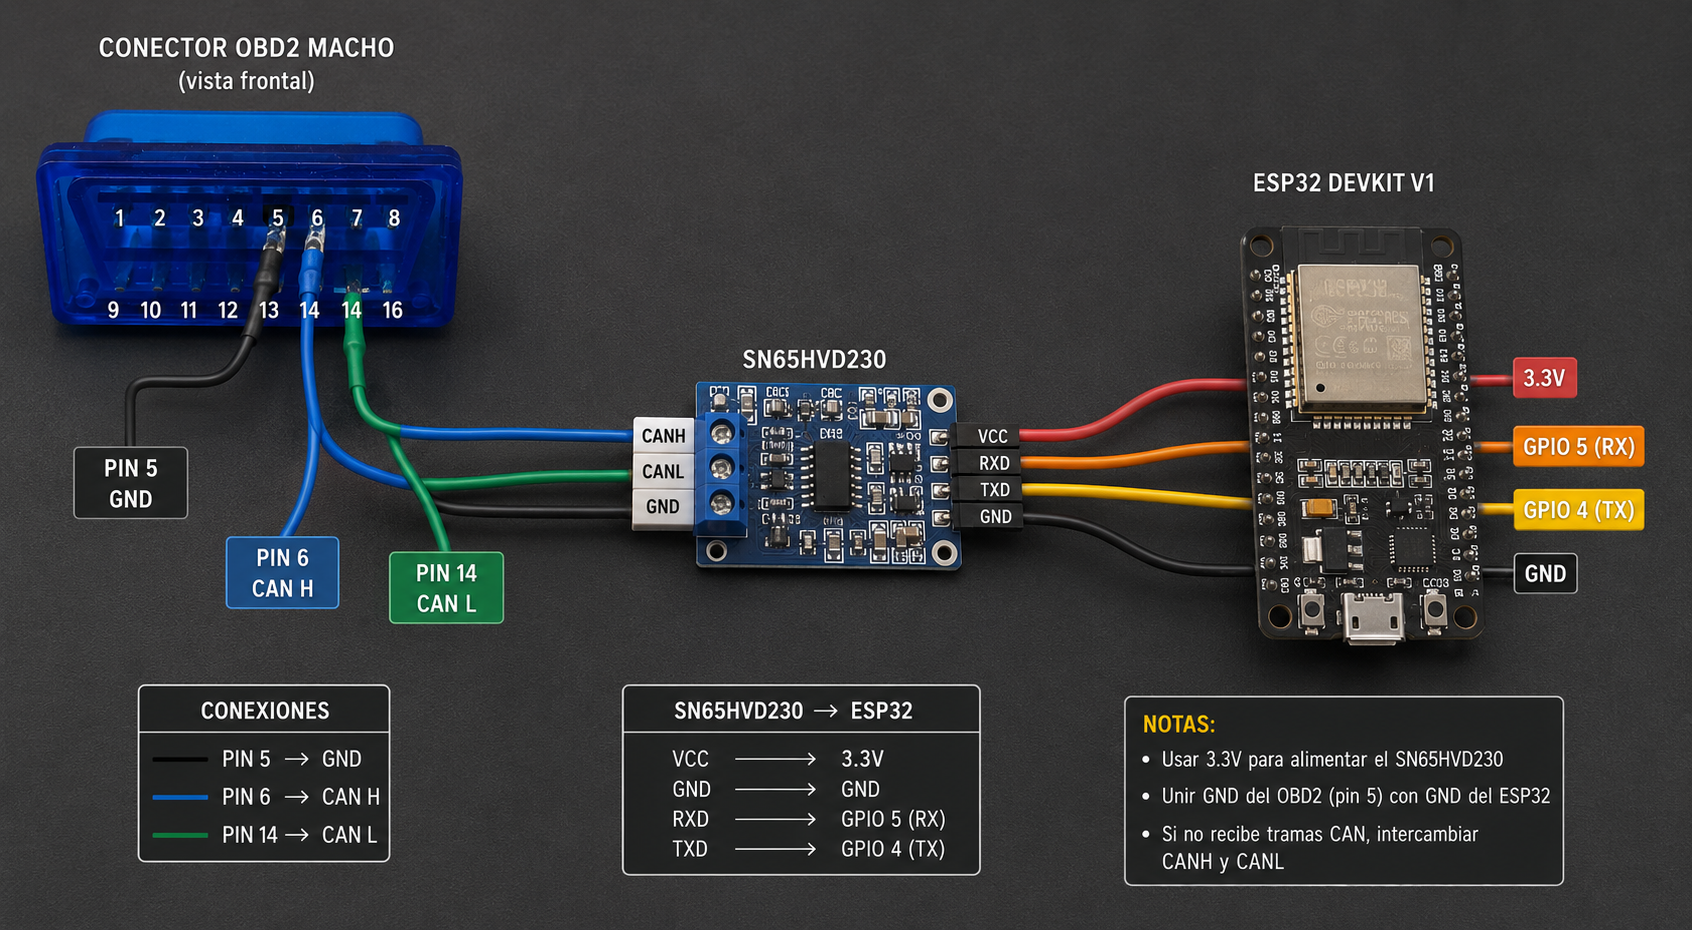
\includegraphics[width=1\textwidth]{Images/REAL.png}
	\vspace{0.2cm}
	
	% La nota explicativa detallada va debajo, alineada a la izquierda
	\begin{flushleft}
		\footnotesize \textit{Nota.} Esquema de conexión entre los componentes de la Tabla \ref{tab:pinout_conexion}. Elaboración propia asistida con IA (Gemini).
	\end{flushleft}
\end{figure}


\subsection{Configuración SLCAN y SavvyCAN para el análisis de datos}

Una vez completada la implementación física del \textit{hardware} de adquisición basado en el ESP32, el siguiente paso crítico es la interfaz lógica con un entorno de análisis. Debido a que las tramas CAN en vehículos como el Changan Honor 2023 operan a velocidades de entre 250 y 500\,kbps, el uso de un monitor serial convencional resulta insuficiente, ya que la alta tasa de datos satura la visualización y dificulta la interpretación en tiempo real.

Para solventar esta limitación, se implementa el protocolo \textbf{SLCAN (Serial CAN)}, basado en el estándar \textit{LAWICEL}. SLCAN permite encapsular tramas CAN dentro de un flujo de datos serie (UART), facilitando que el microcontrolador actúe como un adaptador CAN-USB transparente. Esta arquitectura es fundamental para el uso de \textbf{SavvyCAN}, una herramienta de código abierto especializada en ingeniería inversa, \textit{fuzzing} y análisis de tráfico vehicular, la cual es compatible de forma nativa con el protocolo SLCAN \citep{savvycan2026}.

La Tabla \ref{tab:herramientas_analisis} presenta una comparativa de las herramientas evaluadas para este estudio:

\begin{table}[htbp]
	\centering
	\captionsetup{labelformat=simple, labelsep=newline, textfont=it, labelfont=bf}
	\caption{Comparativa de herramientas de análisis para tráfico CAN}
	\label{tab:herramientas_analisis}
	\begin{tabular}{p{2.5cm} p{2.5cm} p{5cm}}
		\toprule
		\rowcolor[rgb]{0.851, 0.851, 0.851}
		\textbf{Herramienta} & \textbf{Licencia} & \textbf{Características principales} \\
		\midrule
		SavvyCAN & Open Source & Ingeniería inversa, \textit{fuzzing}, soporte SLCAN. \\
		Busmaster & Open Source & Simulación de nodos y redes. \\
		webCAN & Propietario & Visualización web y gráficos rápidos. \\
		CANtact App & Open Source & Sencillez y diagnóstico básico. \\
		\bottomrule
	\end{tabular}
	\vspace{0.2cm}
	\begin{flushleft}
		\small
		\begin{center}
			\textit{Nota.}Elaboración propia.
		\end{center}
		
	\end{flushleft}
\end{table}

Para la ejecución en entornos Linux (Ubuntu), es necesario configurar el puerto serie mediante \textit{udev} o asignar permisos de lectura/escritura al usuario actual sobre el dispositivo (ej. \texttt{/dev/ttyUSB0}). SavvyCAN, al ser ejecutado en Ubuntu, permite la conexión mediante el \textit{Serial/SLCAN Connection Manager}. La configuración recomendada es la siguiente:
\begin{enumerate}
	\item \textbf{Selección de puerto:} Identificar el puerto serie donde está conectado el ESP32.
	\item \textbf{Baudrate:} Configurar el \textit{baudrate} del puerto serie a 115200 o superior (dependiendo del \textit{firmware} del ESP32).
	\item \textbf{Configuración SLCAN:} Habilitar el formato \textit{LAWICEL} y establecer la velocidad del bus CAN (500\,kbps para este caso específico).
\end{enumerate}

La elección de SavvyCAN se justifica por su capacidad de manejar grandes volúmenes de datos con una sobrecarga mínima, permitiendo capturar y filtrar tramas de forma eficiente bajo el protocolo SLCAN \citep{savvycan2026}.

Para que SavvyCAN pueda interpretar estos datos en tiempo real, es necesario utilizar el protocolo slcan a través del puerto serial. Este protocolo emplea una estructura de trama específica con el formato txxxxxxxxxx, la cual permite al software decodificar y mostrar la actividad del bus CAN de manera continua.

Con este objetivo, se configuró el ESP32 mediante un código diseñado para leer los datos recibidos por el transceptor SN65HVD230 (aprovechando los pines dedicados para hardware CAN del microcontrolador) y retransmitirlos hacia SavvyCAN a través del puerto serial.
	
Para la integración del hardware se desarrolló un firmware en el entorno de desarrollo de Arduino utilizando el controlador nativo de dos cables para redes automotrices (TWAI). En la Figura 1 se detalla la lógica de programación orientada a la bidireccionalidad de datos entre el bus del vehículo y el software de análisis de diagnóstico.


\begin{figure}[H]
	\caption{Firmware bidireccional entre el driver TWAI del ESP32 y SavvyCAN.}
	\label{fig:codigo_esp32_slcan}
	
	\begin{lstlisting}[
		language=C++,
		basicstyle=\fontsize{9.5}{9}\ttfamily,
		columns=flexible,
		breaklines=true,
		breakatwhitespace=false,
		postbreak=\mbox{\textcolor{gray}{$\hookrightarrow$}\space}
		]
#include <Arduino.h>
#include "driver/twai.h"

static const gpio_num_t CAN_TX_PIN = GPIO_NUM_4;
static const gpio_num_t CAN_RX_PIN = GPIO_NUM_5;

void handleSavvyCANTransmit(String cmd) {

	if (cmd.length() < 5 || cmd[0] != 't') return;
	twai_message_t tx_msg;
	memset(&tx_msg, 0, sizeof(tx_msg)); 
	tx_msg.identifier = strtol(cmd.substring(1, 4).c_str(), NULL, 16);
	tx_msg.data_length_code = cmd.substring(4, 5).toInt();
	if (tx_msg.data_length_code > 8) tx_msg.data_length_code = 8;
	for (int i = 0; i < tx_msg.data_length_code; i++) {
		tx_msg.data[i] = strtol(cmd.substring(5 + (i * 2), 7 + (i * 2)).c_str(), NULL, 16);
	}
	esp_err_t res = twai_transmit(&tx_msg, pdMS_TO_TICKS(5));
	if (res != ESP_OK) {
	}
}

void setup() {

	Serial.begin(115200); 	
	twai_general_config_t g_config = TWAI_GENERAL_CONFIG_DEFAULT(CAN_TX_PIN, CAN_RX_PIN, TWAI_MODE_NORMAL);
	twai_timing_config_t t_config = TWAI_TIMING_CONFIG_500KBITS(); 
	twai_filter_config_t f_config = TWAI_FILTER_CONFIG_ACCEPT_ALL();
	
	if (twai_driver_install(&g_config, &t_config, &f_config) == ESP_OK) {
		twai_start();
	}
}

void loop() {

	twai_message_t rx_msg;
	while (twai_receive(&rx_msg, 0) == ESP_OK) {
		if (!(rx_msg.flags & TWAI_MSG_FLAG_RTR)) {
			Serial.printf("t03Xd", rx_msg.identifier, rx_msg.data_length_code);
			for (int i = 0; i < rx_msg.data_length_code; i++) {
				Serial.printf("02X", rx_msg.data[i]);
			}
			Serial.print('\r'); 
		}
	}
	
	while (Serial.available()) {
		char c = Serial.read();
		if (c == '\r') {
			handleSavvyCANTransmit(inputBuffer);
			inputBuffer = "";
		} else if (c != '\n') { 
			inputBuffer += c;
		}
	}
}
	\end{lstlisting}
	
	\vspace{-3mm} % Ajuste de espaciado estándar para la nota	
	\small
\textit{Nota.} Algoritmo estructurado para la conversión asíncrona de tramas del bus de datos bajo el estándar \textit{slcan}. Utiliza el retorno de carro (\texttt{\textbackslash r}) con referencia de \citep{ocsaly2022canfuzzer}.
\end{figure}

Después de cargar el firmware al esp32 y montar el circuito planteado en la Figura \ref{fig:obd_conector_soldado} se procede a obtener tramas CAN, los siguientes son usados en el sistema operativo UBUNTU 22.4 para tener mas control de los comunicadores.

\begin{itemize}
	\item Primero se descarga el archivo ejecutable para Ubuntu de SAvvyCAN de la pagina oficial de la misma \citep{savvycan2026}.
	
	\item Posteriormente se conceden permisos al archivo con el siguiente comando por la terminal ver Figura \ref{fig:terminal_instalacion}
	
	\begin{figure}[H]
		\caption{Comando para los permisos de administrador a SavvyCAN.}
		\label{fig:terminal_instalacion}
		
		\begin{lstlisting}[style=terminal, basicstyle=\fontsize{11}{13}\ttfamily\color{white}]
			$ sudo chmod +x SavvyCAN-x86_64.AppImage
			$ sudo ./SavvyCAN-x86_64.AppImage 
		\end{lstlisting}
		
		\vspace{2mm}
		\textit{Nota.} Secuencia de comandos ejecutada en terminal Bash sobre Ubuntu 22.04 para la instalación y apertura del software SAvvyCAN.
	\end{figure}
	
	\item Después se observa que el software se abre y queda listo para recibir las tramas.
	
	\item Mientras cargamos el código de la Figura \ref{fig:codigo_esp32_slcan} igual atravesar de la terminal al ESP32 con el comando de la Figura \ref{fig:comando_upload_esp32}.
	
	\begin{figure}[H]
		\caption{Comando para la carga del firmware al microcontrolador ESP32 mediante PlatformIO.}
		\label{fig:comando_upload_esp32}
		
		\begin{lstlisting}[style=terminal, basicstyle=\fontsize{11}{13}\ttfamily\color{white}]
			$ pio run --target upload --upload-port /dev/ttyUSB0
		\end{lstlisting}
		
		\vspace{2mm}
		\textit{Nota.} Comando ejecutado en terminal Bash sobre Ubuntu 22.04. El puerto \texttt{/dev/ttyUSB0} corresponde a la conexión serial del ESP32; puede variar según el sistema. Se requiere tener PlatformIO CLI instalado y el archivo \texttt{platformio.ini} configurado en el directorio del proyecto.
	\end{figure}
	
	\item  A continuación se conecta al SavvyCAN con la siguiente configuración como se ve en la Figura \ref{fig:config_savvyCAN}.
	
	\begin{figure}[H]
		\centering
		% El título y número se integran en el \caption (arriba de la imagen en APA)
		\caption{Configuración en el software SavvyCAN}
		\label{fig:config_savvyCAN}
		
		\vspace{0.3cm}
		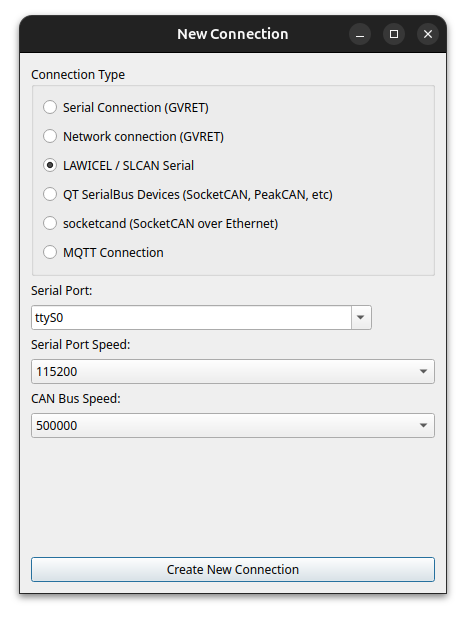
\includegraphics[width=0.8\textwidth]{Images/Savvy.png}
		\vspace{0.2cm}
		
		% La nota explicativa detallada va debajo, alineada a la izquierda
		\begin{flushleft}
			\footnotesize \textit{Nota.} Configuración de la conexión en SavvyCAN mediante el protocolo SLCAN, utilizando un ESP32 como puente serial hacia el bus CAN.
		\end{flushleft}
	\end{figure}
	
	\item Después de crear la conexión podremos notar como las tramas can se muestran en la pantalla como se ve en la Figura \ref{fig:imagencan}.
	
		\begin{figure}[H]
		\centering
		% El título y número se integran en el \caption (arriba de la imagen en APA)
		\caption{Conexion exitosa con el software SavvyCAN}
		\label{fig:imagencan}
		
		\vspace{0.3cm}
		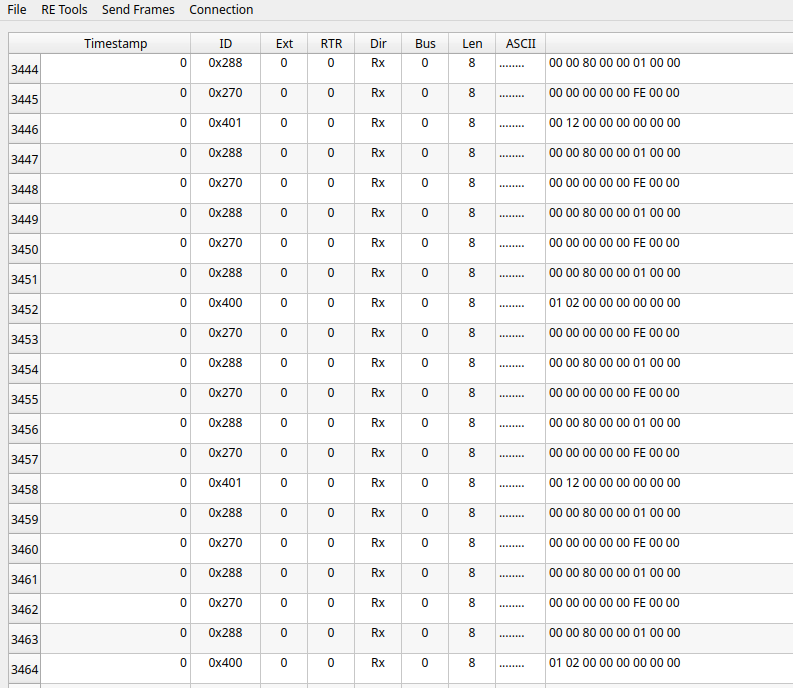
\includegraphics[width=1\textwidth]{Images/capturaCAN.png}
		\vspace{0.2cm}
		
		% La nota explicativa detallada va debajo, alineada a la izquierda
		\begin{flushleft}
			\footnotesize \textit{Nota.} Se detalla como los valores en hexadecimal están en cambio porque el vehículo al estar en contacto recibe muchas tramas CAN.
		\end{flushleft}
	\end{figure}
	
	\item Finalmente se demuestra exitosamente que si existen estas tramas CAN y en la siguiente parte veremos sus análisis y compresión del mismo.
	
\end{itemize}

\subsection{Análisis de tramas capturadas}
% Presentar capturas reales de SavvyCAN.
% Tabla con IDs CAN observados, periodicidad y longitud.
% Figura: screenshot de SavvyCAN con tramas reales.

Una vez establecida la comunicación con el vehículo (cuya arquitectura puede compararse con la de un sistema robótico compuesto por múltiples subsistemas interconectados), se procedió a la captura de tramas del bus de datos.

Como se observa en la Figura \ref{fig:imagencan}, los valores 
obtenidos en bruto no resultan interpretables de forma directa, por lo 
que es necesario aplicar ingeniería inversa para descifrar el significado 
de cada parámetro. Con base en los PIDs normalizados presentados en la 
Tabla \ref{tab:PID}, se identificaron en primera instancia aquellos 
parámetros conocidos como punto de partida para el análisis.

\subsubsection{Identificación de IDs}
% ID 0x7DF (broadcast), 0x7E8 (respuesta ECU principal).
% Diferencia entre tramas de diagnóstico y tramas nativas.
Para este análisis, se utilizó la herramienta Sniffer integrada en SavvyCAN, la cual permite monitorear e identificar en tiempo real las variaciones en los datos del bus. Un ejemplo práctico de su aplicación consiste en la conmutación de las luces altas del vehículo. Como se observa en la Figura \ref{fig:Sniffer}, la interfaz resalta dinámicamente los cambios en los bytes: los valores decrecientes se tiñen de color rojo, mientras que aquellos que se incrementan se muestran en verde, facilitando así la detección visual de las transiciones de datos.

\begin{figure}[htbp]
	\centering
	% 1. Forzamos el contador manual para que \ref{fig:Sniffer} extraiga el número exacto
	\refstepcounter{figure}
	\label{fig:Sniffer}
	
	% 2. Estructura de Título APA 7 (Alineado a la izquierda)
	\begin{flushleft}
		\bfseries Figura \thefigure \\
		\normalfont\itshape Interfaz de la herramienta Sniffer en SavvyCAN para el monitoreo del bus
	\end{flushleft}
	\vspace{2mm} % Espacio entre el título y la imagen
	
	% 3. Inserción de la Imagen (Cambia 'tu_imagen_sniffer' por el nombre de tu archivo)
	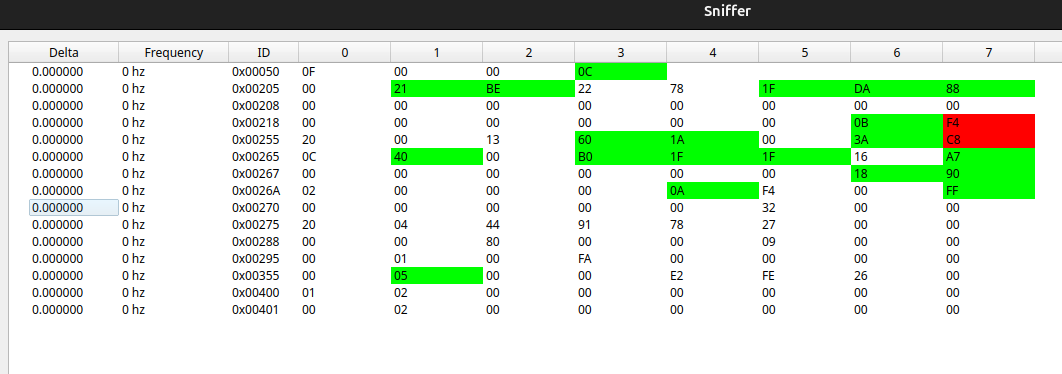
\includegraphics[width=1.0\textwidth]{Images/Sniffer.png} 
	
	\vspace{2mm} % Espacio entre la imagen y la nota
	
	% 4. Nota de Figura APA 7 (Alineada a la izquierda y en tamaño pequeño)
	\begin{flushleft}
		\itshape Nota. \normalfont Monitoreo pasivo en tiempo real de los identificadores de CAN (CAN IDs). La interfaz destaca dinámicamente las variaciones de los bytes empleando un código de colores: verde para incrementos en los valores y rojo para decrementos.
	\end{flushleft}
\end{figure}

Este procedimiento es fundamental para el proceso de ingeniería inversa; por ejemplo, al activar las luces de parqueo, se examinan las modificaciones en el Sniffer con el objetivo de aislar e identificar el identificador de CAN (CAN ID) y la trama hexadecimal específica que comanda dicha función.

Posteriormente, se analizó el comportamiento de las revoluciones por minuto (RPM) del motor en SavvyCAN. Aunque el estándar OBD-II define conceptualmente el PID 0x0C para solicitar de forma activa las RPM (como se listó en la Tabla A1 del Apéndice A), mediante el escaneo pasivo (Sniffer) se identificó que el vehículo transmite de forma autónoma estos datos bajo el CAN ID como muestra su estructura en la Figura \ref{fig:CAN_Frame}. Para validar este hallazgo, se capturaron las tramas en tiempo real bajo diferentes regímenes de operación (ver Figura \ref{fig:RPM_SNIFFER}).

\begin{figure}[htbp]
	\centering
	% 1. Forzamos el contador manual para que \ref{fig:RPM_SNIFFER} extraiga el número exacto
	\refstepcounter{figure}
	\label{fig:RPM_SNIFFER}
	
	% 2. Estructura de Título APA 7 (Alineado a la izquierda)
	\begin{flushleft}
		\bfseries Figura \thefigure \\
		\normalfont\itshape Monitoreo del bus CAN a un régimen constante de 2000 RPM
	\end{flushleft}
	\vspace{2mm} % Espacio entre el título y la imagen
	
	% 3. Inserción de la Imagen (Cambia 'tu_imagen_rpm_2000' por tu archivo correspondiente)
	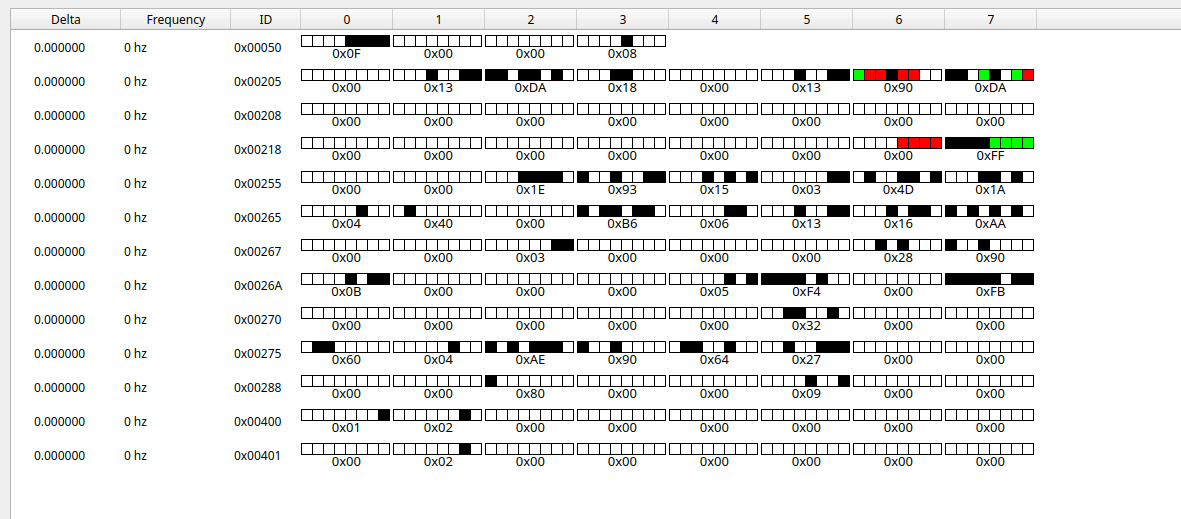
\includegraphics[width=1.0\textwidth]{Images/rpm_sniffer.png} 
	
	\vspace{2mm} % Espacio entre la imagen y la nota
	
	% 4. Nota de Figura APA 7 (Alineada a la izquierda y en tamaño pequeño)
	\begin{flushleft}
		\itshape Nota. \normalfont Captura de datos en el software SavvyCAN con el motor retenido a 2000 RPM. Las variaciones cromáticas en los bytes del ID \texttt{0x00255} permiten aislar las señales dinámicas vinculadas a la velocidad angular del cigüeñal del motor frente al estado de ralentí.
	\end{flushleft}
\end{figure}

Utilizando los datos crudos extraídos en un instante específico de la captura, se aplicaron las ecuaciones de ingeniería inversa correspondientes para decodificar los bytes y comparar el resultado matemático con el valor reflejado simultáneamente en el tacómetro del tablero de instrumentos del vehículo.

La ecuación matemática estándar que rige esta conversión, considerando la resolución universal de $0{,}25\,\text{RPM}/\text{bit}$ (factor de división por 4), se define en la Ecuación~\ref{eq:rpm_standard}:

\begin{equation}
	\text{RPM} = \frac{(\text{MSB} \times 256) + \text{LSB}}{4}
	\label{eq:rpm_standard}
\end{equation}

Donde $\text{MSB}$ representa el Byte Más Significativo (\textit{Byte Alto}) y $\text{LSB}$ representa el Byte Menos Significativo (\textit{Byte Bajo}).

\subsubsection{Candidato 1: ID \texttt{0x00255} (Bytes 2 y 3)}
A partir de la captura en vivo con el motor retenido, los bytes en estado activo para este ID presentaron los valores hexadecimales $\text{Byte}_2 = 1\text{E}_{16}$ y $\text{Byte}_3 = 93_{16}$. Convirtiendo dichos valores a base decimal se obtiene:
\begin{itemize}
	\item $\text{MSB} = 1\text{E}_{16} = (1 \times 16^1) + (14 \times 16^0) = 30$
	\item $\text{LSB} = 93_{16} = (9 \times 16^1) + (3 \times 16^0) = 147$
\end{itemize}

Sustituyendo estos valores en la ecuación de ingeniería inversa:
\begin{equation}
	\text{RPM}_{0255} = \frac{(30 \times 256) + 147}{4} = \frac{7680 + 147}{4} = \frac{7827}{4} = \mathbf{1956{,}75\,\text{RPM}}
\end{equation}

\subsubsection{Candidato 2: ID \texttt{0x00218} (Bytes 6 y 7)}
Este ID mostró alta volatilidad durante la aceleración. Evaluando sus bytes finales, cuyos valores registrados fueron $\text{Byte}_6 = 00_{16}$ y $\text{Byte}_7 = \text{FF}_{16}$, se procede con la conversión decimal:
\begin{itemize}
	\item $\text{MSB} = 00_{16} = 0$
	\item $\text{LSB} = \text{FF}_{16} = 255$
\end{itemize}

Sustituyendo en la ecuación fundamental:
\begin{equation}
	\text{RPM}_{0218} = \frac{(0 \times 256) + 255}{4} = \frac{255}{4} = \mathbf{63{,}75\,\text{RPM}}
\end{equation}

\subsubsection{Candidato 3: ID \texttt{0x00275} (Bytes 1 y 2)}
Este identificador, vinculado tentativamente a la posición del acelerador, marcó variaciones lineales leves. Tomando sus primeros bytes modificados, $\text{Byte}_1 = 00_{16}$ y $\text{Byte}_2 = \text{AE}_{16}$, se calcula su equivalente decimal:
\begin{itemize}
	\item $\text{MSB} = 00_{16} = 0$
	\item $\text{LSB} = \text{AE}_{16} = (10 \times 16^1) + (14 \times 16^0) = 174$
\end{itemize}

Sustituyendo en la ecuación:
\begin{equation}
	\text{RPM}_{0275} = \frac{(0 \times 256) + 174}{4} = \frac{174}{4} = \mathbf{43{,}50\,\text{RPM}}
\end{equation}

\subsubsection{Comparación de Resultados y Validación}

En la Tabla~\ref{tab:comparativa_ids} se organizan los datos calculados frente al valor real de referencia observado en el tacómetro analógico del vehículo ($2000\,\text{RPM}$).

\begin{table}[htbp]
	\centering
	\captionsetup{labelformat=simple, labelsep=newline, textfont=it, labelfont=bf}
	\caption{Comparativa de IDs candidatos para la determinación de la variable de RPM}
	\label{tab:comparativa_ids}
	% Definimos anchos fijos (p) que suman 14.0cm en total para una distribución perfecta en la hoja
	\begin{tabular}{p{1.8cm} p{2.5cm} p{2.8cm} p{3.8cm} p{3.1cm}}
		\toprule
		\rowcolor[rgb]{0.851, 0.851, 0.851}
		\textbf{CAN ID} & \textbf{Datos Hexadecimales} & \textbf{Valor Calculado} & \textbf{Desviación Absoluta} & \textbf{¿Es el ID de RPM?} \\
		\midrule
		\texttt{0x00255} & \texttt{0x1E 0x93} & \textbf{1956{,}75 RPM} & \textbf{43{,}25 RPM (2.1\%)} & \textbf{SÍ (Confirmado)} \\
		\texttt{0x00218} & \texttt{0x00 0xFF} & 63{,}75 RPM            & 1936{,}25 RPM                & NO \\
		\texttt{0x00275} & \texttt{0x00 0xAE} & 43{,}50 RPM            & 1956{,}50 RPM                & NO \\ 
		\bottomrule
	\end{tabular}
	\vspace{0.2cm}
	\begin{flushleft}
		\small
		\begin{center}
			\textit{Nota.} Comparativa de los identificadores del bus CAN analizados bajo un régimen constante de operación frente al valor nominal del tacómetro. Elaboración propia.
		\end{center}
	\end{flushleft}
\end{table}

A partir del análisis comparativo, se determina que el identificador del bus CAN perteneciente a las revoluciones por minuto es contundentemente el \textbf{ID \texttt{0x00255}}. 

La resolución matemática arroja un valor de $1956{,}75\,\text{RPM}$, lo cual representa una precisión del $97{,}9\%$ respecto al valor objetivo visualizado en el tablero de instrumentos.

El margen de desviación residual ($\approx 2{,}1\%$) no manifiesta un error en el modelado de la ecuación, sino que responde al comportamiento dinámico real del motor de combustión interna, cuyas micro-oscilaciones son captadas de forma pura por el bus de datos en milisegundos, mientras que la aguja física del cuadro de instrumentos actúa como un filtro mecánico amortiguado que suaviza la lectura visual para el conductor.

Los resultados demuestran que, mediante el análisis por ingeniería inversa de los identificadores (IDs) provistos por la herramienta SavvyCAN, es posible aislar e interpretar la estructura de las tramas CAN del vehículo.

\subsection{Selección final de PIDs para monitoreo de consumo}
% Justificar por qué se eligieron los 12 PIDs de la Tabla~\ref{tab:pids}.
% Tabla comparativa: PID disponible en Changan Honor vs Nissan Vanette.
% Criterio de conmutación MAF → Speed-Density si 0x10 no responde.
A continuación, se abordará la consulta de Identificadores de Parámetro (PIDs). A diferencia de los identificadores de trama (IDs) del bus CAN, que definen pasivamente la procedencia o prioridad de un mensaje, los PIDs constituyen peticiones activas enviadas hacia la Unidad de Control Electrónico (ECU), la cual procesa la solicitud y devuelve la información bajo un esquema de pregunta-respuesta. Este mecanismo interactivo representa el principio operativo fundamental de la mayoría de los escáneres automotrices comerciales. Con el propósito de determinar qué variables de telemetría están disponibles en el vehículo de prueba, se desarrolló inicialmente un algoritmo general diseñado para explorar y decodificar el mapa de bits de los PIDs soportados.

El código fuente en C++ presentado en la Figura \ref{fig:codigo_scanner_obd2} implementa la inicialización, inyección y lectura de datos sobre el bus CAN del vehículo. Este algoritmo configura el periférico nativo TWAI \citep{espressif_esp32_datasheet} a un régimen de 500 kbps para garantizar la sincronización temporal con la red automotriz a través del transceptor físico \citep{sn65hvd230_datasheet}. 

El procesamiento de datos se sintetiza en tres etapas operativas esenciales:
\begin{itemize}
	\item \textbf{Inicialización:} En la rutina \texttt{setup()}, se asignan los pines de control (GPIO 4 y 5) y se establece un filtro de aceptación total para habilitar la escucha completa del tráfico en el bus.
	\item \textbf{Transmisión Funcional:} La función \texttt{solicitarPIDsSoportados()} inyecta una trama de diagnóstico única (\textit{Single Frame}) bajo el identificador estándar \texttt{0x7DF} conforme a la norma ISO 15765-4 \citep{iso15765}. La solicitud invoca al Servicio 01 y al PID \texttt{0x00}, rellenando los bytes restantes con ceros (\textit{padding}) para mantener la simetría obligatoria de 8 bytes.
	\item \textbf{Filtrado Lógico:} En el bucle principal \texttt{loop()}, el sistema evalúa las tramas entrantes en el búfer. El algoritmo descarta el tráfico secundario y aísla exclusivamente las respuestas de la ECU de motor (\texttt{0x7E8}) que validen el servicio (\texttt{0x41 0x00}), extrayendo finalmente los 4 bytes del mapa de bits.
\end{itemize}

\begin{figure}[H]
	\caption{Algoritmo en C++ para la detección activa y decodificación del mapa de bits de PIDs soportados en el bus CAN.}
	\label{fig:codigo_scanner_obd2}
	
	\begin{lstlisting}[
		language=C++,
		basicstyle=\fontsize{9.5}{9}\ttfamily,
		columns=flexible,
		breaklines=true,
		breakatwhitespace=false,
		postbreak=\mbox{\textcolor{gray}{$\hookrightarrow$}\space}
		]
#include "driver/twai.h"
#define CAN_TX_PIN GPIO_NUM_5
#define CAN_RX_PIN GPIO_NUM_4

void setup() {
	Serial.begin(115200);
	while(!Serial);
	Serial.println("Iniciando Escaner de PIDs OBD-II...");
	twai_general_config_t g_config = TWAI_GENERAL_CONFIG_DEFAULT(CAN_TX_PIN, CAN_RX_PIN, TWAI_MODE_NORMAL);
	twai_timing_config_t t_config = TWAI_TIMING_CONFIG_500KBITS(); 
	twai_filter_config_t f_config = TWAI_FILTER_CONFIG_ACCEPT_ALL();
	if (twai_driver_install(&g_config, &t_config, &f_config) == ESP_OK) {
		Serial.println("Driver TWAI instalado con exito.");
	} else {
		while (1);
	}
	if (twai_start() == ESP_OK) {
		Serial.println("Driver TWAI iniciado.");
	} else {
		while (1);
	}
	delay(2000);
	solicitarPIDsSoportados();
}
void loop() {
	twai_message_t rx_msg;
	if (twai_receive(&rx_msg, pdMS_TO_TICKS(1000)) == ESP_OK) {
		// Filtrar respuestas OBD2 estandar (0x7E8) y Servicio 01
		if (rx_msg.identifier == 0x7E8 && rx_msg.data[1] == 0x41 && rx_msg.data[2] == 0x00) {
			Serial.print("Respuesta Recibida de la ECU ID: 0x");
			Serial.println(rx_msg.identifier, HEX);
			Serial.print("Mapa de bits de PIDs (Hex): ");
			for(int i = 3; i < 7; i++) {
				if(rx_msg.data[i] < 0x10) Serial.print("0");
				Serial.print(rx_msg.data[i], HEX);
				Serial.print(" ");
			}
			Serial.println("\n-----------------------------------------");}}
}
void solicitarPIDsSoportados() {
	twai_message_t tx_msg;
	tx_msg.identifier = 0x7DF; 
	tx_msg.extd = 0;           
	tx_msg.data_length_code = 8;
	tx_msg.data[0] = 0x02;     
	tx_msg.data[1] = 0x01;     
	tx_msg.data[2] = 0x00;     
	for(int i=3; i<8; i++) tx_msg.data[i] = 0x00; 	
	if (twai_transmit(&tx_msg, pdMS_TO_TICKS(1000)) == ESP_OK) {
		Serial.println("Solicitud PID 0x00 enviada correctamente.");
	}}		
	\end{lstlisting}
	
	\vspace{-3mm} % Ajuste de espaciado estándar para la nota	
	\small
	\textit{Nota.} Algoritmo estructurado para la inicialización y el control del periférico de comunicación automotriz mediante la inyección activa de tramas de diagnóstico funcional (ID \texttt{0x7DF}). Desarrollado a partir de las especificaciones de bajo nivel para el manejo del buffer y sincronización de bits con referencias de \citep{espressif_twai} y \citep{sae_j1979_2014}.
\end{figure}


% ==========================================
% SECCIÓN 3: RESULTADOS EN MONITOR SERIE
% ==========================================
\subsubsection{Resultados Obtenidos}
Tras compilar el código y conectar el sistema al puerto OBD-II del Changan Honor con el contacto en posición \textit{ON}, el monitor serie arrojó la siguiente salida a $115200\text{ baudios}$ ver Figura \ref{fig:monitor_serie_obd2}:

\begin{figure}[H]
	\caption{Captura de pantalla del monitor serie durante la ejecución del escáner de PIDs OBD-II (Changan Honor).}
	\label{fig:monitor_serie_obd2}
	\centering
	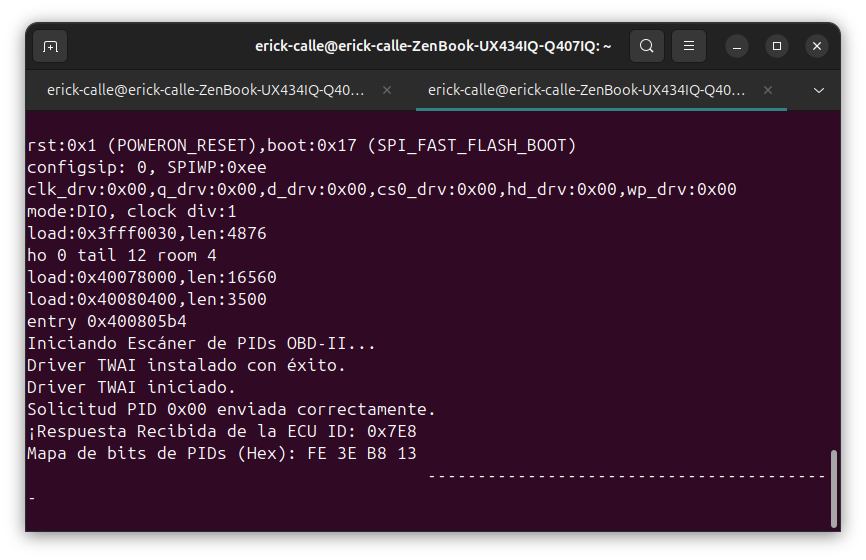
\includegraphics[width=0.85\textwidth]{Images/Serial.png} % Reemplaza por el nombre de tu archivo de imagen
	
	\vspace{2mm} % Ajuste de espaciado para la nota bajo formato APA
	\textit{Nota.} Registro de depuración en tiempo real, tomado sobre el Changan Honor, que muestra la inicialización correcta del controlador TWAI, el envío de la solicitud funcional (PID 0x00) y la respuesta hexadecimal (\texttt{FE 3E B8 13}) emitida por la unidad de control del motor (ECU).

\end{figure}

% ==========================================
% SECCIÓN 4: INTERPRETACIÓN DE RESULTADOS
% ==========================================
\subsubsection{Interpretación de Resultados}

La respuesta del bus CAN indica que la comunicación bidireccional fue exitosa. El identificador \texttt{0x7E8} confirma, bajo la arquitectura de segmentación de IDs de diagnóstico físico \cite{iso15765}, que la trama proviene directamente del módulo de control del motor (ECM).

Para determinar la disponibilidad de los comandos, el mapa de bits devuelto en formato hexadecimal, \texttt{FE 3E B8 13}, debe ser descompuesto en su representación binaria de 32 bits. Siguiendo el estándar SAE J1979 \citep{sae_j1979_2014}, cada bit se evalúa de izquierda a derecha (desde el bit más significativo hasta el menos significativo), donde un estado lógico de 1 indica que el PID está soportado por la ECU, y un estado de 0 indica su ausencia.

A continuación, se detalla la conversión de los cuatro bytes y el mapeo completo de los bits correspondientes al primer bloque de diagnóstico (PIDs del 0x01 al 0x20):
\begin{itemize}
	\item \textbf{Byte 1 (\texttt{FE}):} \texttt{1111 1110} $\rightarrow$ Soportados PIDs del 0x01 al 0x07; el PID 0x08 está ausente.
	\item \textbf{Byte 2 (\texttt{3E}):} \texttt{0011 1110} $\rightarrow$ Ausentes PIDs 0x09 y 0x0A; soportados del 0x0B al 0x0F; el PID 0x10 está ausente.
	\item \textbf{Byte 3 (\texttt{B8}):} \texttt{1011 1000} $\rightarrow$ Soportados PIDs 0x11, 0x13, 0x14 y 0x15; los demás están ausentes.
	\item \textbf{Byte 4 (\texttt{13}):} \texttt{0001 0011} $\rightarrow$ Soportados PIDs 0x1C, 0x1F y 0x20; los demás están ausentes.
\end{itemize}

La Tabla~\ref{tab:mapeo_pids_binario} describe la función específica y el impacto analítico de las variables críticas recuperadas en este mapa de bits para la caracterización dinámica del tren motriz.

\begin{table}[htbp]
	\centering
	\captionsetup{labelformat=simple, labelsep=newline, textfont=it, labelfont=bf}
	\caption{Mapeo binario de la respuesta hexadecimal FE 3E B8 13 y descripción de PIDs}
	\label{tab:mapeo_pids_binario}
	\small
	\renewcommand{\arraystretch}{1.3}
	% Definimos anchos fijos (p) que suman 14.2cm para mantener simetría exacta con tus otras tablas
	\begin{tabular}{p{1.5cm} p{1.2cm} p{2.2cm} p{3.0cm} p{6.3cm}}
		\toprule
		\rowcolor[rgb]{0.851, 0.851, 0.851}
		\textbf{Byte} & \textbf{Hex} & \textbf{Binario} & \textbf{PID Asociado} & \textbf{Descripción Técnica Resumida} \\
		
		Byte 1 & \texttt{FE} & \texttt{1111111\textbf{0}} & PID 0x01 - 0x08 & Estado de monitores y códigos de falla (DTC). \\
		&             &                            & \textbf{PID 0x0B (1)} & \textbf{MAP:} Presión del múltiple de admisión; clave para la densidad del aire. \\
		&             &                            & \textbf{PID 0x0C (1)} & \textbf{RPM:} Régimen de giro del motor y ciclos de llenado. \\ 
		
		Byte 2 & \texttt{3E} & \texttt{00\textbf{111110}} & \textbf{PID 0x0D (1)} & \textbf{VSS:} Velocidad del vehículo; convierte el consumo a L/km. \\
		&             &                            & \textbf{PID 0x0F (1)} & \textbf{IAT:} Temperatura de admisión; corrige la densidad por factor térmico. \\
		&             &                            & \texttt{PID 0x10 (0)} & \textbf{MAF:} Sensor de flujo de masa de aire (Ausente). \\ 
		
		Byte 3 & \texttt{B8} & \texttt{10111000}          & PID 0x11 - 0x18       & Posición del acelerador y sensores de oxígeno activos. \\ 
		
		Byte 4 & \texttt{13} & \texttt{00010011}          & PID 0x19 - 0x20       & Tiempo de operación y habilitación del bloque 0x21-0x40. \\
		\bottomrule
	\end{tabular}
	\vspace{0.2cm}
	\begin{flushleft}
		\small
		\begin{center}
			\textit{Nota.} El bit final del Byte 4 (\texttt{PID 0x20 = 1}) confirma que la ECU admite la consulta del siguiente rango de parámetros (PIDs 0x21 a 0x40) para expandir la adquisición de datos.
		\end{center}
	\end{flushleft}
\end{table}

% ==========================================
% SECCIÓN 5: CONCLUSIÓN DE LA PRUEBA
% ==========================================
\subsubsection{Conclusión de la prueba}

La ausencia absoluta del sensor MAF (\texttt{PID 0x10 = 0}), combinada con la disponibilidad simultánea y mandatoria de los sensores MAP, RPM e IAT, revela un aspecto fundamental de la arquitectura de la ECU: el sistema de inyección electrónica del vehículo no mide el flujo de aire de forma masiva directa, sino que calcula el caudal utilizando el método indirecto de Densidad de Velocidad (\textit{Speed Density}).

Este hallazgo define y valida el desarrollo matemático del sistema embebido. Al no contar con el PID 0x10, el microcontrolador deberá ser programado para resolver la ecuación de estado de los gases ideales combinada con la eficiencia volumétrica del motor en tiempo real. Al disponer de los datos de presión (MAP), temperatura (IAT) y velocidad angular (RPM), se confirma que el hardware desarrollado tiene acceso a todas las variables de estado requeridas para modelar el flujo de aire y estimar el consumo instantáneo de combustible de manera matemática y precisa.

El mismo procedimiento de escaneo se repitió sobre el segundo vehículo de prueba (Nissan Vanette), confirmando además que este sí soporta el PID 0x10 (MAF), tal como se resume en la Tabla~\ref{tab:pids_verificacion} del Capítulo~4. El listado completo y decodificado de los PIDs soportados por ambos vehículos se presenta en el Apéndice~O.
% ────────────────────────────────────────────────────────────
\section{Selección y justificación de componentes}
% Tu sección actual, sin cambios de fondo.
% Evalúa opciones → justifica → tabla resumen de componentes.
En esta sección se describen los componentes seleccionados para el sistema, priorizando su disponibilidad local en la ciudad de La Paz y su alineación con los objetivos del proyecto. La elección se basa en criterios de compatibilidad eléctrica, facilidad de integración, costo y rendimiento, con énfasis en soluciones robustas y accesibles.

\subsection{Interfaz OBD-II y controlador CAN}
% Conector, TJA1050 vs SN65HVD230, MCP2515.
Para leer datos del puerto OBD-II del vehículo, se requiere una conexión estable al bus CAN (Controller Area Network). Los componentes clave son:

\begin{enumerate}
	\item \textbf{Conector OBD-II}: Se utiliza un conector extraído de un escáner defectuoso para garantizar fiabilidad. Alternativamente, dos cables directos a las líneas CANH y CANL podrían emplearse, pero presentan riesgos de falsos contactos o conexiones inestables.Este posteriormente sera remplazado para una versión final del sistema.
	
	\item \textbf{Transceptores CAN}: Para convertir las señales diferenciales CANH/CANL en líneas digitales RX/TX compatibles con el microcontrolador, se evaluaron dos opciones:
	\begin{itemize}
		\item TJA1050 : Actúa como transceptor bidireccional, convirtiendo señales eléctricas del bus CAN en RX/TX como muestra en la Tabla B1 del Apéndice B. Es de bajo costo y disponible. Y su rango de voltajes de señal nos da el primer obstáculo como se ve en la Tabla B2 del Apéndice B al no ser de rango 3{,}3~V.
		
		\item SN65HVD230 (ver Apéndice C): Similar al anterior, pero optimizado para 3{,}3\,V; ideal, entonces, para microcontroladores de bajo voltaje.
		
	\end{itemize}
	Se seleccionó el SN65HVD230 por su stock local, popularidad en aplicaciones automotrices y compatibilidad con 3{,}3~V.
	
	\item \textbf{Controlador CAN (Periférico TWAI)}: Se seleccionó el ESP32 como unidad central debido a que integra periféricamente un controlador CAN a nivel de silicio, una característica ausente en la mayoría de microcontroladores convencionales de desarrollo ver Apéndice D. Este módulo nativo asume de forma autónoma la gestión de la capa de enlace de datos: empaqueta el payload, ejecuta el filtrado de mensajes por hardware para no saturar la CPU y administra la corrección de errores. 
\end{enumerate}

A todo esto se descartó el uso del escáner ELM327 de código abierto por su mayor costo y dependencia de conectividad inalámbrica (Bluetooth/Wi-Fi), que requeriría un ESP32 o Raspberry Pi con Python/MicroPython, complicando la integración.

\subsection{Microcontrolador del Sistema}
A diferencia de los esquemas de procesamiento distribuido, el núcleo de este sistema centraliza la adquisición de datos, el modelado matemático y la conectividad inalámbrica en un único circuito integrado, optimizando el espacio físico y suprimiendo la latencia de comunicación inter-procesador:

\begin{itemize}
	\item \textbf{ESP32}: Seleccionado como la unidad central de control debido a su arquitectura de alto rendimiento y su versatilidad periférica. El dispositivo asume de forma nativa dos funciones críticas para el proyecto: la gestión del bus CAN automotriz mediante su controlador interno TWAI (\textit{Two-Wire Automotive Interface}) y la transmisión inalámbrica de la telemetría hacia el servidor local a través de su pila de protocolos Wi-Fi integrada. 
\end{itemize}

\subsection{Periféricos de visualización}
% LCD 20×4 con módulo I2C vs OLED. Selección y justificación.
Se evaluaron varias pantallas para mostrar datos en tiempo real, priorizando tamaño, facilidad de conexión (I$^2$C o paralelo) y legibilidad para conductores:

\begin{itemize}

	\item \textbf{Pantalla LCD 20x4 o 16x2 }: Ofrece el tamaño óptimo para datos vehiculares, mejorando la usabilidad sin sacrificar simplicidad.
	
	\item \textbf{Pantalla OLED}: Se selecciono esta por ser compacta, conexión I$^2$C simple y compatible con 3{,}3~V según el Apéndice E.
	
\end{itemize}

\subsection{Lenguaje de programación}

El lenguaje de programación seleccionado es C++, por ser mas optimo para su programación y flexibilidad en entornos embebidos.

Finalmente en la Tabla \ref{tab:componentes_seleccionados} se muestran los componentes seleccionados :

\begin{table}[H]
	\centering
	\captionsetup{labelformat=simple, labelsep=newline, textfont=it, labelfont=bf, justification=raggedright, singlelinecheck=false}
	\caption{Componentes seleccionados y justificación técnica del sistema unificado}
	\label{tab:componentes_seleccionados}
	\small
	\renewcommand{\arraystretch}{1.3}
	% Mantenemos tus anchos fijos calibrados (3.5cm + 3.2cm + 7.5cm = 14.2cm) para un ajuste perfecto
	\begin{tabular}{p{3.5cm} p{3.2cm} p{7.5cm}}
		\toprule
		\rowcolor[rgb]{0.851, 0.851, 0.851}
		\textbf{Componente} & \textbf{Selección} & \textbf{Ventajas y justificación en el proyecto} \\ 
		\midrule
		Interfaz OBD-II & Conector OBD-II estándar & Permite una conexión mecánica y eléctrica estable directamente con el puerto de diagnóstico del vehículo. \\
		
		Microcontrolador y Controlador CAN & ESP32 & Centraliza el procesamiento, el modelado matemático de consumo y la conectividad Wi-Fi. Su periférico nativo TWAI elimina la necesidad de chips controladores externos como el MCP2515. \\ 
		
		Transceptor CAN & SN65HVD230 & Opera nativamente a 3,3 V, acoplándose de forma segura a los pines del ESP32. Traduce las señales lógicas a los niveles diferenciales del bus CAN automotriz. \\ 
		
		Pantalla de visualización & OLED & Ofrece excelente legibilidad en entornos con alta iluminación solar y mejor adaptación a ser 3,3 V. \\
		
		Lenguaje de programación & C++ (Entorno Arduino) & Cuenta con librerías maduras y de bajo nivel para el manejo del periférico TWAI, optimizando el tiempo de desarrollo y la estabilidad del sistema embebido. \\
		\bottomrule
	\end{tabular}
	\vspace{0.2cm}
	\begin{flushleft}
		\small
		\begin{center}
			\textit{Nota.} Arquitectura de hardware optimizada y simplificada a partir de la centralización de procesos en un único núcleo de ejecución.
		\end{center}
	\end{flushleft}
\end{table}
% ────────────────────────────────────────────────────────────
\section{Diseño de hardware}

\subsection{Módulo de Interfaz CAN Bus (SN65HVD230 + ESP32)}

El transceptor SN65HVD230 de Texas Instruments fue seleccionado como interfaz física 
entre el microcontrolador ESP32 y el bus CAN del vehículo. A diferencia de soluciones 
basadas en el MCP2515, este transceptor no requiere controlador CAN externo ni 
comunicación SPI, dado que el ESP32 integra nativamente el periférico 
TWAI\textsuperscript{\textregistered} (\textit{Two-Wire Automotive Interface}), 
compatible con el estándar ISO 11898-1 (CAN 2.0B). La conexión entre ambos 
dispositivos se reduce a dos líneas lógicas: TX y RX entre el ESP32 y el 
transceptor, y dos líneas diferenciales CANH y CANL hacia el bus del vehículo.

\subsubsection{Configuración del Periférico TWAI\textsuperscript{\textregistered} del ESP32}

La velocidad del bus CAN automotriz opera típicamente a 500~kbps bajo el estándar 
ISO 11898-1. La configuración del periférico TWAI\textsuperscript{\textregistered} 
se realiza directamente mediante el driver oficial de Espressif en el framework 
ESP-IDF, sin necesidad de calcular registros de temporización manualmente. 
La inicialización del bus se estructura en tres parámetros fundamentales, 
tal como se muestra en la Figura \ref{fig:twai_init}:

\begin{figure}[H]
	\caption{Inicialización del periférico TWAI\textsuperscript{\textregistered} 
			del ESP32 a 500~kbps.}
	\label{fig:twai_init}
	\begin{lstlisting}[language=C++, basicstyle=\fontsize{10}{10}\ttfamily, breaklines=true]
twai_general_config_t g_config = 
TWAI_GENERAL_CONFIG_DEFAULT(GPIO_NUM_4, GPIO_NUM_5, TWAI_MODE_NORMAL);
twai_timing_config_t t_config = TWAI_TIMING_CONFIG_500KBITS();
twai_filter_config_t f_config = TWAI_FILTER_CONFIG_ACCEPT_ALL();
		
twai_driver_install(&g_config, &t_config, &f_config);
twai_start();
	\end{lstlisting}
	\vspace{-1mm}
	\noindent\small\textit{Nota.} La macro \texttt{TWAI\_TIMING\_CONFIG\_500KBITS()} 
	configura automáticamente los parámetros de bit-timing (TQ, PropSeg, PhaseSeg1, 
	PhaseSeg2 y SJW) para operar a 500~kbps sobre el reloj interno del ESP32 
	a 80~MHz, eliminando el cálculo manual de registros CNF.
\end{figure}

\subsubsection{Filtrado de Tramas CAN por Identificador}

El periférico TWAI\textsuperscript{\textregistered} incorpora un filtro de 
aceptación por hardware configurable mediante una máscara de 32 bits, equivalente 
funcional a los registros RXF y RXM del MCP2515. Para recibir únicamente la 
respuesta de la ECU principal en consultas OBD-II (ID \texttt{0x7E8}), se 
configura el filtro de la siguiente manera (ver Figura \ref{fig:twai_filter}):

\begin{figure}[H]
	\caption{Configuración del filtro de aceptación para recepción exclusiva 
			de respuestas OBD-II.}
	\label{fig:twai_filter}
	\begin{lstlisting}[language=C++, basicstyle=\fontsize{10}{10}\ttfamily, breaklines=true]
twai_filter_config_t f_config = {
	.acceptance_code = (0x7E8 << 21), // ID aceptado: respuesta ECU
	.acceptance_mask = ~(0x7FF << 21), // Mascara exacta de 11 bits
	.single_filter   = true
};
	\end{lstlisting}
	\vspace{-1mm}
	\noindent\small\textit{Nota.} El desplazamiento de 21 bits se debe al formato 
	interno del registro de filtro del TWAI\textsuperscript{\textregistered}, que 
	ubica el identificador de 11 bits en los bits más significativos de la palabra 
	de 32 bits. La máscara \texttt{0x7FF} garantiza coincidencia exacta del 
	identificador, descartando cualquier otra trama presente en el bus y reduciendo 
	la carga de procesamiento del sistema.
\end{figure}

\subsection{Módulo de Visualización (OLED I2C)}

Para la visualización local de parámetros se empleó una pantalla OLED de 
128$\times$64 píxeles controlada mediante el protocolo I2C, conectada 
directamente al ESP32. La dirección esclava del dispositivo es \texttt{0x3C}, 
configurable a \texttt{0x3D} mediante el puente de soldadura en la placa del 
módulo. La gestión del display se realizó mediante la biblioteca 
\texttt{Adafruit\_SSD1306}, que abstrae el protocolo de comunicación y provee 
funciones de renderizado de texto y gráficos primitivos.

\subsubsection{Distribución de la información en pantalla}

A diferencia de un esquema de múltiples pantallas navegables, el firmware mantiene una única pantalla fija que se redibuja por completo cada \texttt{OLED\_REFRESH\_PERIOD\_MS} (400~ms por defecto), priorizando en todo momento los datos que más se consultan al conducir: el consumo y el costo acumulado del viaje. La distribución de la información en esa pantalla se detalla en la Tabla \ref{tab:distribucion_pantallas}.

\begin{table}[H]
	\centering
	\captionsetup{labelformat=simple, labelsep=newline, textfont=it, labelfont=bf, justification=raggedright, singlelinecheck=false}
	\caption{Distribución de la información en la pantalla OLED}
	\label{tab:distribucion_pantallas}
	\small
	\renewcommand{\arraystretch}{1.3}
	% Mantenemos la calibración exacta de anchos fijos (3.0cm + 11.2cm = 14.2cm)
	\begin{tabular}{p{3.0cm} p{11.2cm}}
		\toprule
		\rowcolor[rgb]{0.851, 0.851, 0.851}
		\textbf{Zona} & \textbf{Contenido mostrado} \\
		\midrule
		Línea superior & RPM del motor (PID \texttt{0x0C}) y velocidad del vehículo (PID \texttt{0x0D}), en texto pequeño. \\

		Centro (texto grande) & Consumo instantáneo: L/100~km si el vehículo se mueve (velocidad $>2$~km/h), o L/h si está detenido o en ralentí, para no dividir entre una velocidad cercana a cero. \\

		Centro (texto grande) & Costo acumulado del viaje, en bolivianos, calculado a partir del combustible ya consumido (\texttt{trip\_fuel\_L} $\times$ \texttt{FUEL\_PRICE\_BS\_PER\_L}), no de la tasa instantánea. \\

		Línea inferior 1 & Distancia y combustible acumulados del viaje. \\

		Línea inferior 2 & Estado de la comunicación CAN (\texttt{CAN:OK}/\texttt{CAN:--}) y estado del panel web: dirección IP del punto de acceso si está activo, o \texttt{srv:--} en caso contrario. \\
		\bottomrule
	\end{tabular}
	\vspace{0.2cm}
	\begin{flushleft}
		\small
		\begin{center}
			\textit{Nota.} No hay navegación entre pantallas ni pulsador físico asociado a la OLED: toda la información relevante para conducir se muestra simultáneamente en esta única vista, y el detalle adicional (MAP, IAT, eficiencia volumétrica, flujo de aire y combustible calculados, etc.) queda disponible en el panel web y en el registro de la tarjeta microSD (Tabla~\ref{tab:estructura_csv}).
		\end{center}
	\end{flushleft}
\end{table}

\subsection{Módulo de Registro en Memoria (SSD)}

Para el almacenamiento persistente de los datos adquiridos se utilizó una 
memoria de estado sólido conectada al ESP32 mediante el protocolo SPI. 
Los registros se almacenan en formato CSV con marca de tiempo, permitiendo 
su posterior análisis en herramientas de ofimática o procesamiento de datos.
Cada sesión genera un archivo independiente identificado por número de 
sesión correlativo, preservando el historial completo de adquisiciones.

\subsubsection{Estructura del Archivo de Registro}

Cada fila del archivo CSV registra una muestra completa de los parámetros 
activos en ese instante, con la estructura definida en la Tabla \ref{tab:estructura_csv}.

\begin{table}[H]
	\centering
	\captionsetup{labelformat=simple, labelsep=newline, textfont=it, labelfont=bf, justification=raggedright, singlelinecheck=false}
	\caption{Estructura real del registro CSV escrito por \texttt{sdLoggerTask()} (\texttt{sd\_logger.cpp})}
	\label{tab:estructura_csv}
	\small
	\renewcommand{\arraystretch}{1.15}
	% Mantenemos la calibración exacta de anchos fijos (3.5cm + 2.0cm + 8.7cm = 14.2cm)
	\begin{tabular}{p{3.5cm} p{2.0cm} p{8.7cm}}
		\toprule
		\rowcolor[rgb]{0.851, 0.851, 0.851}
		\textbf{Campo} & \textbf{Tipo} & \textbf{Descripción} \\
		\midrule
		\texttt{uptime\_ms}       & uint32 & Tiempo transcurrido desde el arranque del sistema, en milisegundos (\texttt{millis()}). \\
		\texttt{rpm}              & uint16 & Revoluciones por minuto del motor (PID \texttt{0x0C}). \\
		\texttt{speed\_kmh}       & float  & Velocidad del vehículo, en km/h (PID \texttt{0x0D}). \\
		\texttt{map\_kpa}         & float  & Presión absoluta del colector de admisión, en kPa (PID \texttt{0x0B}). \\
		\texttt{iat\_c}           & float  & Temperatura del aire de admisión, en °C (PID \texttt{0x0F}). \\
		\texttt{coolant\_c}       & float  & Temperatura del líquido refrigerante del motor, en °C (PID \texttt{0x05}). \\
		\texttt{ve\_pct}          & float  & Eficiencia volumétrica interpolada de \texttt{kVeTable} para el régimen actual, en \%. \\
		\texttt{maf\_gs}          & float  & Flujo másico de aire estimado por el modelo Speed-Density, en g/s. \\
		\texttt{fuel\_gs}         & float  & Flujo másico de combustible calculado, en g/s. \\
		\texttt{instant\_Lh}      & float  & Consumo instantáneo en L/h (válido en ralentí o vehículo detenido). \\
		\texttt{instant\_L100km}  & float  & Consumo instantáneo en L/100~km (válido con el vehículo en movimiento). \\
		\texttt{trip\_km}         & float  & Distancia acumulada del viaje, en km. \\
		\texttt{trip\_fuel\_L}    & float  & Combustible acumulado del viaje, en L. \\
		\texttt{trip\_avg\_L100km} & float & Consumo promedio acumulado del viaje, en L/100~km. \\
		\texttt{can\_status}      & uint8  & Estado de la comunicación CAN (\texttt{0}=INIT, \texttt{1}=OK, \texttt{2}=SIN\_RESPUESTA, \texttt{3}=ERROR\_BUS, \texttt{4}=BUS\_OFF). \\
		\texttt{trip\_cost\_bs}   & float  & Costo acumulado del viaje, en bolivianos (\texttt{trip\_fuel\_L}~$\times$~\texttt{FUEL\_PRICE\_BS\_PER\_L}). \\
		\texttt{baro\_kpa}        & float  & Presión barométrica de referencia, en kPa (PID \texttt{0x33} real, o estimación del modelo ISA si no está soportado). \\
		\texttt{baro\_is\_estimated} & bool & \texttt{1} si \texttt{baro\_kpa} proviene de la estimación ISA; \texttt{0} si es una lectura real por PID \texttt{0x33}. \\
		\bottomrule
	\end{tabular}
	\vspace{0.2cm}
	\begin{flushleft}
		\small
		\begin{center}
			\textit{Nota.} Fila exacta escrita cada \texttt{SD\_LOG\_INTERVAL\_MS} (1000~ms por defecto) mientras hay una lectura CAN válida; el archivo se abre una sola vez por sesión y cada fila se escribe en modo \textit{append} con \texttt{flush()} inmediato, de forma que una pérdida de energía no descarta filas ya escritas. Los ajustes de combustible STFT/LTFT (PIDs \texttt{0x06}/\texttt{0x07}) se usan internamente para corregir el cálculo (Capítulo~3, lazo cerrado) pero no se registran como columnas propias de este CSV.
		\end{center}
	\end{flushleft}
\end{table}


\subsection{Módulo de Comunicación Inalámbrica y Servidor Web}

El mismo ESP32 que gestiona la adquisición CAN opera simultáneamente como 
punto de acceso WiFi (\textit{Access Point}), exponiendo un servidor web 
embebido para la visualización remota de parámetros en tiempo real desde 
cualquier dispositivo conectado a la red local generada. No se requiere 
conexión a internet ni infraestructura de red externa.

\subsubsection{Arquitectura del Servidor Web Embebido}

El servidor web se implementó con la biblioteca \texttt{ESPAsyncWebServer}, 
que permite atender peticiones HTTP y mantener conexiones WebSocket de forma 
asíncrona sin bloquear el bucle principal de adquisición CAN. La interfaz 
gráfica HTML/CSS/JS se almacena en la partición SPIFFS del ESP32 y se sirve 
estáticamente al cliente. La actualización de datos en tiempo real se realiza 
mediante WebSocket, evitando el \textit{polling} HTTP y reduciendo la latencia 
de visualización. El flujo de datos completo se ilustra en la 
Figura~\ref{fig:flujo_web}.

\begin{figure}[htbp]
	\centering
	% Título alineado a la izquierda estilo APA 7 idéntico a tus tablas
	\captionsetup{labelformat=simple, labelsep=newline, textfont=it, labelfont=bf, justification=raggedright, singlelinecheck=false}
	\caption{Flujo de datos desde el bus CAN hasta el cliente web}
	\label{fig:flujo_web}
	
	\begin{tikzpicture}[
		% Configuración de Estilos de los Bloques
		node_ext/.style={rectangle, draw=gray!70!black, fill=gray!5, thick, rounded corners=3pt, text width=5.2cm, align=center, minimum height=0.9cm, font=\small},
		node_core1/.style={rectangle, draw=blue!60!black, fill=blue!4, thick, rounded corners=3pt, text width=5.2cm, align=center, minimum height=0.9cm, font=\small},
		node_core0/.style={rectangle, draw=teal!60!black, fill=teal!4, thick, rounded corners=3pt, text width=5.2cm, align=center, minimum height=0.9cm, font=\small},
		node_hw/.style={rectangle, draw=gray!50, fill=gray!1, dashed, rounded corners=3pt, text width=3.4cm, align=center, minimum height=0.9cm, font=\small},
		arrow/.style={-{Stealth[scale=1.2]}, draw=black!70, thick}
		]
		
		% --- UBICACIÓN DE NODOS ---
		
		% Origen externo
		\node (can) [node_ext] {\textbf{Bus CAN (Vehículo)}};
		
		% Bloque del Núcleo 1 (Adquisición y Almacenamiento)
		\node (twai) [node_core1, below=0.8cm of can] {\textbf{ESP32 - Núcleo 1}\\Periférico TWAI\\(Adquisición CAN)};
		
		% Periféricos locales de salida (a los lados del Núcleo 1)
		\node (oled) [node_hw, left=0.7cm of twai] {\textbf{OLED I2C}\\(Visualización local)};
		\node (ssd) [node_hw, right=0.7cm of twai] {\textbf{SSD SPI}\\(Registro CSV persistente)};
		
		% Bloques del Núcleo 0 (Conectividad y Servidor Web)
		\node (ap) [node_core0, below=1.0cm of twai] {\textbf{ESP32 - Núcleo 0}\\Access Point WiFi\\(192.168.4.1)};
		
		\node (web) [node_core0, below=0.6cm of ap] {\textbf{ESPAsyncWebServer}\\HTTP $\rightarrow$ \texttt{index.html} (SPIFFS)};
		
		\node (ws) [node_core0, below=0.6cm of web] {\textbf{WebSocket}\\Transmisión de datos \texttt{JSON}};
		
		% Destino final (Entorno del cliente)
		\node (nav) [node_ext, below=1.0cm of ws] {\textbf{Navegador Cliente}\\(Renderizado en Laptop/Móvil)};
		
		\node (chart) [node_ext, below=0.6cm of nav] {\textbf{Canvas nativo}\\Gráficas en tiempo real};
		
		% --- CONEXIONES / FLECHAS ---
		
		\draw [arrow] (can) -- (twai);
		\draw [arrow] (twai) -- (oled);
		\draw [arrow] (twai) -- (ssd);
		
		% Enlace inter-núcleos
		\draw [arrow] (twai) -- (ap) node[midway, right, font=\scriptsize\itshape, text=black!60] {Memoria compartida};
		
		\draw [arrow] (ap) -- (web);
		\draw [arrow] (web) -- (ws);
		
		% Transmisión inalámbrica hacia el cliente
		\draw [arrow] (ws) -- (nav) node[midway, right, font=\scriptsize\itshape, text=black!60] {Enlace WiFi (WebSockets)};
		
		\draw [arrow] (nav) -- (chart);
		
	\end{tikzpicture}
	
	\vspace{0.2cm}
	\begin{flushleft}
		\small
		\begin{center}
			\textit{Nota.} Todos los módulos operan sobre el mismo microcontrolador ESP32, aprovechando el núcleo dual del procesador: el núcleo 0 gestiona la comunicación WiFi y el servidor web, mientras que el núcleo 1 ejecuta la adquisición CAN y la escritura en SSD.
		\end{center}
	\end{flushleft}
\end{figure}
\subsubsection{Formato de Trama JSON por WebSocket}

Cada 500~ms el ESP32 serializa los parámetros activos en un objeto JSON 
y lo transmite a todos los clientes conectados mediante difusión 
(\textit{broadcast}) WebSocket con la estructura en código como se muestra en la Figura \ref{fig:json_trama}:

\begin{figure}[H]
	\caption{Estructura de la trama JSON transmitida por WebSocket 
			al cliente web.}
	\label{fig:json_trama}
	\begin{lstlisting}[language=C++, basicstyle=\fontsize{10}{10}\ttfamily, breaklines=true]
// Serializacion en el ESP32
String buildJSON(OBDData& d) {
	return "{\"rpm\":"      + String(d.rpm, 0)       +
		",\"vel\":"      + String(d.velocidad)     +
		",\"temp\":"     + String(d.temp_ref)      +
		",\"carga\":"    + String(d.carga, 1)      +
		",\"maf\":"      + String(d.maf, 2)        +
		",\"stft\":"     + String(d.stft_b1, 1)    +
		",\"ltft\":"     + String(d.ltft_b1, 1)    +
		",\"ts\":"       + String(millis())        + "}";
}
		
// Envio broadcast a todos los clientes WebSocket
ws.textAll(buildJSON(currentData));
	\end{lstlisting}
	\vspace{-3mm}
	\noindent\small\textit{Nota.} El cliente web recibe el JSON y actualiza 
	las gráficas mediante Chart.js sin recargar la página, logrando una 
	visualización fluida con latencia inferior a 100~ms en condiciones normales 
	de red local.
\end{figure}

\subsection{Diagrama esquemático general}
% Tu contenido actual: 4 bloques funcionales con figuras.
En esta sección se presentará el diseño esquemático del sistema, realizando el cálculo y selección de los valores óptimos para cada componente con base en las recomendaciones de sus respectivas hojas de datos. Para facilitar el análisis y diseño, el sistema se ha dividido en los siguientes subsistemas:

\begin{itemize}
	
	\item \textbf{Sistema de alimentación:} En este subsistema se incorporarán las etapas de protección, regulación y filtrado de energía. Su principal objetivo es garantizar una alimentación estable y segura para todos los componentes del sistema, minimizando los efectos de ruido eléctrico, interferencias y transitorios de tensión.
	
	\item \textbf{Sistema transceptor CAN:} Se analizará el funcionamiento del transceptor CAN SN65HVD230, implementando una configuración optimizada que permita reducir el espacio ocupado en la PCB y mantener una comunicación confiable con la red CAN del vehículo.
	
	\item \textbf{Sistema de procesamiento:} Comprende el microcontrolador ESP32 y todos los componentes necesarios para su correcto funcionamiento, incluyendo circuitos auxiliares, interfaces de comunicación y conexiones para los distintos periféricos del sistema.
	
	\item \textbf{Sistema de visualización:} Se desarrollará la interfaz de conexión hacia una pantalla externa ubicada en el tablero del vehículo, para que el usuario disponga de la información relevante.

	\item \textbf{Sistema de almacenamiento de datos:} Se implementará una interfaz para memoria microSD destinada al almacenamiento de los datos obtenidos por el sistema, de modo que puedan analizarse y procesarse más adelante.

	\item \textbf{Sistema de programación:} Incluye los componentes necesarios para la configuración, programación y actualización del firmware del ESP32; con esto se simplifica el desarrollo y mantenimiento del dispositivo.
	
	\item \textbf{Sistema de monitoreo y estado:} Se incorporarán indicadores luminosos (LEDs) que permitirán visualizar el estado operativo del sistema y facilitar tareas de diagnóstico durante su funcionamiento.
	
\end{itemize}

Todos estos subsistemas han sido concebidos para su implementación en una placa de circuito impreso (PCB). A continuación, se desarrollan los esquemáticos correspondientes a cada uno de ellos.


\subsubsection{Sistema de alimentación}

Se contempla la obtención del voltaje de alimentación principal directamente desde el pin 16 del conector OBD-II del vehículo, el cual proporciona una tensión nominal de 12~V proveniente de la batería (ver Figura \ref{fig:pinobd}). Debido a que los circuitos electrónicos internos operan a tensiones significativamente menores, es indispensable implementar una etapa previa de acondicionamiento, protección y reducción de voltaje mediante un convertidor reductor (\textit{step-down}). 

Con el propósito de mitigar perturbaciones eléctricas severas comunes en el entorno automotriz, tales como transitorios de conmutación o picos de tensión, se diseñó una etapa de protección robusta previa a la regulación síncrona a niveles de 5~V y 3{,}3~V. El flujo lógico y secuencial planificado para esta etapa de potencia se detalla en la Figura \ref{fig:esquema_potencia}.

\begin{figure}[H]
	\centering
	% Formato APA 7 con alineación estricta a la izquierda y protección para el índice
	\captionsetup{labelformat=simple, labelsep=newline, textfont=it, labelfont=bf, justification=raggedright, singlelinecheck=false}
	\caption[Diagrama de bloques del sistema de protección y regulación de energía (12V a 3.3V)]{Diagrama de bloques del sistema de protección y regulación de energía}
	\label{fig:esquema_potencia}
	
	% Escalamos el diagrama automáticamente para que ocupe el ancho del texto
	\resizebox{\textwidth}{!}{%
		\begin{tikzpicture}[
			% Configuración de estilos visuales para las etapas
			etapa_in/.style={rectangle, draw=red!60!black, fill=red!5, thick, rounded corners=3pt, text width=2.4cm, align=center, minimum height=1.1cm, font=\small},
			etapa_prot/.style={rectangle, draw=gray!70!black, fill=gray!5, thick, rounded corners=3pt, text width=2.4cm, align=center, minimum height=1.1cm, font=\small},
			etapa_reg/.style={rectangle, draw=orange!70!black, fill=orange!5, thick, rounded corners=3pt, text width=2.4cm, align=center, minimum height=1.1cm, font=\small},
			etapa_out/.style={rectangle, draw=teal!70!black, fill=teal!4, thick, rounded corners=3pt, text width=2.4cm, align=center, minimum height=1.1cm, font=\small},
			arrow/.style={-{Stealth[scale=1.2]}, draw=black!70, thick}
			]
			
			% --- UBICACIÓN HORIZONTAL DE LOS BLOQUES ---
			\node (pin16) [etapa_in] {\textbf{Pin 16 (12V)}\\Entrada OBD-II};
			
			\node (fuse) [etapa_prot, right=0.5cm of pin16] {\textbf{Fusible}\\Protección contra sobrecorriente};
			
			\node (diode) [etapa_prot, right=0.5cm of fuse] {\textbf{Diodo TVS}\\Supresión de picos de voltaje};
			
			% Conexión directa del TVS al Buck de 3.3V
			\node (reg33v) [etapa_reg, right=0.5cm of diode] {\textbf{Regulador 5V}\\(TPS54302 Buck)};
			
			\node (esp32) [etapa_out, right=0.5cm of reg33v] {\textbf{ESP32}\\y Periféricos 3,3V};
			
			% --- CONEXIONES / FLECHAS ---
			\draw [arrow] (pin16) -- (fuse);
			\draw [arrow] (fuse) -- (diode);
			\draw [arrow] (diode) -- (reg33v) node[midway, below, font=\scriptsize\bfseries\color{black!60}] {12V};
			\draw [arrow] (reg33v) -- (esp32) node[midway, below, font=\scriptsize\bfseries\color{black!60}] {5V};
			
		\end{tikzpicture}%
	}
	
	\vspace{3mm}
	\small\raggedright
	\textit{Nota.} Topología de conversión directa de alta eficiencia basada en el regulador síncrono TPS54302. Esta configuración reduce directamente la tensión del bus automotriz de 12~V a 3{,}3~V nominales, optimizando la disipación térmica y garantizando un suministro eléctrico estable para el microcontrolador y sus periféricos críticos, previniendo caídas de tensión (\textit{brownouts}) bajo las exigencias de consumo del transmisor Wi-Fi \cite{espressif_esp32_datasheet}.
\end{figure}

Con base en el diagrama de bloques estructurado, se procedió a la selección rigurosa de los
componentes electrónicos para la etapa de potencia. Esta etapa es crítica para adaptar los 12~V
nominales provenientes del pin 16 del conector OBD-II a los niveles lógicos del sistema,
garantizando fiabilidad frente a las exigentes condiciones eléctricas del entorno automotriz:

\begin{enumerate}
	
	\item \textbf{Fusible rearmable (PTC):} Debido a que la red eléctrica del vehículo está
	expuesta a cortocircuitos y sobrecorrientes transitorias, se descartó el uso de fusibles
	tradicionales de un solo uso. Se optó por el fusible rearmable polimérico PTC modelo
	LUTE 1812L150/33GR, el cual soporta una tensión máxima de operación de 33~V, una corriente
	de mantenimiento (\textit{hold current}) de 1{,}5~A y una corriente de disparo
	(\textit{trip current}) de 3{,}0~A en encapsulado SMD 1812,datos que muestra la hoja de datos del componente en el Apendice F \citep{bourns_bsmd1812}. Su
	principal ventaja radica en su capacidad de restablecer automáticamente la conducción una
	vez que la falla desaparece y el componente se enfría, eliminando la necesidad de
	reemplazo físico en el campo.
	
	\item \textbf{Diodo Schottky de protección de polaridad inversa (D1):} Para evitar daños
	irreversibles ante una conexión accidental con polaridad invertida en el puerto OBD-II, se
	integró el diodo Schottky SS34 en serie con la línea de alimentación positiva. Según su
	hoja de datos mostrada en el Apéndice G , este componente soporta una tensión inversa repetitiva máxima
	($V_{RRM}$) de 40~V y una corriente media rectificada ($I_O$) de 3~A, con una caída de
	tensión directa típica de 550~mV a plena carga \citep{onsemi_ss36}. Su encapsulado
	DO-214AB (SMA) ofrece excelente disipación térmica en condiciones de alta corriente.
	
	\item \textbf{Diodo TVS (\textit{Transient Voltage Suppressor}):} Para suprimir el ruido
	electromagnético y proteger la circuitería contra picos de voltaje severos (tales como
	los transitorios de desconexión de carga, o \textit{load dump}, propios del entorno
	automotriz, que pueden superar los 40~V) se integró el diodo TVS unidireccional SMAJ18A
	en paralelo con la línea de alimentación, inmediatamente después del fusible PTC y el
	diodo de polaridad. De acuerdo con su hoja de datos (ver Apéndice H), su tensión de trabajo
	(\textit{stand-off voltage}) de 18~V permite la libre operación del voltaje nominal de
	la batería del vehículo, mientras que su tensión de sujeción máxima (\textit{clamping
		voltage}) de 29{,}2~V a una corriente de pico de 13{,}7~A \citep{vishay_smaj28a} garantiza
	que ningún transitorio destructivo alcance al regulador.  La potencia de disipación de pulso pico es de
	400~W con una forma de onda de 10/1000~µs, suficiente para absorber los transitorios
	definidos por la norma ISO 7637-2 en entornos automotrices.
	
	\item \textbf{Regulador reductor de 5~V (TPS54302):} Inicialmente se evaluaron
	reguladores lineales clásicos como el AMS1117-3.3, pero fueron descartados debido a su
	ineficiente disipación térmica al intentar reducir directamente tensiones del bus
	automotriz de 12~V a 3{,}3~V, ya que esto representaría disipar más del 72\% de la potencia
	en calor. En su lugar, se seleccionó el convertidor reductor síncrono
	(\textit{buck converter}) TPS54302 de Texas Instruments.
	
	Este integrado opera en un rango de tensión de entrada de 4{,}5~V a 28~V, entrega una corriente de salida continua de hasta 3~A, y opera a una frecuencia de conmutación fija de 400~kHz (con espectro expandido para reducción de EMI). Incorpora dos MOSFETs de canal N integrados, de bajo $R_{DS(on)}$ (85~m$\Omega$ en el lado alto o \textit{high-side}, y 40~m$\Omega$ en el lado bajo o \textit{low-side}), y con ello configura un convertidor \textit{buck} síncrono, además de una función de modo Eco (\textit{Eco-mode}) que maximiza la eficiencia en condiciones de carga ligera. El rango de temperatura de juntura de operación es de $-40$~°C a $+125$~°C (ver Apéndice I). Se encuentra disponible en encapsulado SOT-23-6, de fácil soldadura y montaje en superficie.
	
	\textbf{Cálculo de la tensión de salida:} La tensión de salida se programa mediante un
	divisor resistivo conectado al pin FB del integrado. Según la hoja de datos del
	TPS54302DDCR, la tensión de referencia interna es $V_{ref} = 0{,}596$~V, y la expresión
	que gobierna la tensión de salida es:
	
	\begin{equation}
		V_{out} = V_{ref} \times \left(1 + \frac{R_{upper}}{R_{lower}}\right)
		\label{eq:vout}
	\end{equation}
	
	Para obtener una salida de 5~V se seleccionaron los valores de resistencia
	$R_{upper} = 100~\text{k}\Omega$ y $R_{lower} = 13{,}3~\text{k}\Omega$. Sustituyendo en
	la ecuación~\ref{eq:vout}:
	
	\begin{equation}
		V_{out} = 0{,}596 \times \left(1 + \frac{100000}{13300}\right) = 0{,}596 \times 8{,}519
		\approx 5{,}078~\text{V}
	\end{equation}
	
	Este valor representa un error del $+1{,}56$\% respecto al valor nominal de 5~V, dentro
	de la tolerancia aceptable para alimentar la etapa posterior de reguladores lineales
	(AMS1117-3.3 y AP2112K-3.3), que a su vez entregan la tensión regulada de 3{,}3~V
	requerida por el microcontrolador ESP32-S3, cuyo rango de operación es de 3{,}0~V a
	3{,}6~V \citep{espressif_esp32_datasheet}.
	
	\textbf{Habilitación (EN):} A diferencia de otros reguladores de la familia TPS543xx
	que permiten configurar un \textit{undervoltage lockout} (UVLO) ajustable mediante un
	divisor resistivo externo en el pin EN, el TPS54302DDCR habilita la conmutación
	simplemente dejando el pin EN sin conexión (\textit{floating}), según lo indicado en su
	hoja de datos. En esta condición, el dispositivo inicia la conmutación de forma
	automática cuando la tensión de entrada supera el umbral interno de UVLO, típicamente
	4{,}5~V, sin necesidad de componentes adicionales. Esta configuración fue la adoptada en
	el diseño, dado que la tensión de entrada protegida (\texttt{12V\_PROT}) proveniente del
	riel del vehículo (12~V a 14{,}4~V nominales) se mantiene ampliamente por encima de este
	umbral durante la operación normal del sistema.
	

	\item \textbf{Filtro de salida LC:} El filtro de salida está compuesto por un inductor de 10~µH y dos condensadores de 22~µF en paralelo, formando una inductancia total de 10~µH y una capacitancia de salida efectiva de 44~µF. Esta combinación proporciona la atenuación del rizado de corriente y tensión necesaria para garantizar una alimentación limpia y estable al microcontrolador ESP32-S3 y demás periféricos del sistema.

	\item \textbf{Compensación del lazo de control:} A diferencia de otros reguladores de la familia TPS543xx que requieren una red de compensación externa tipo II en un pin COMP dedicado, el TPS54302DDCR emplea control en modo de corriente pico (\textit{peak	current-mode control}) con una red de compensación interna optimizada de fábrica. Esto elimina la necesidad de componentes externos de compensación, reduce el conteo de piezas y simplifica el diseño del lazo de control, según lo indicado en su hoja de datos. Como complemento al filtro de salida, se incorporó un condensador adicional de 75~pF en paralelo, cuya función es mejorar la respuesta ante transitorios de carga.
	
	\item \textbf{Regulación de 5~V a 3.3~V:} Para mejorar la eficiencia del convertidor DC-DC la regulación de 5~V a 3.3~V se realizara con 2 componentes muy usados los cuales se detallan:
	\begin{itemize}
		\item \textbf{AMS1117-3.3}
		
		Se seleccionó el regulador AMS1117-3.3 para alimentar exclusivamente el módulo ESP32 debido a su capacidad de suministrar hasta 1 A (ver Apéndice J)de corriente, proporcionando un margen suficiente para soportar los picos de consumo generados por el microcontrolador durante la transmisión Wi-Fi, el funcionamiento del servidor web local y el procesamiento de datos provenientes del sistema OBD-II. Aunque el consumo promedio del ESP32 es inferior, durante las comunicaciones inalámbricas puede presentar picos de corriente superiores a 400 mA, por lo que disponer de un regulador con mayor capacidad mejora la estabilidad del sistema y reduce la posibilidad de caídas de tensión.
		
		\item \textbf{AP2112K-3.3TRG1}
		
		El regulador AP2112K-3.3TRG1 fue destinado a la alimentación de los dispositivos periféricos, como la pantalla OLED, la memoria microSD y otros circuitos auxiliares. Este regulador puede suministrar hasta 600 mA (ver Apéndice K), corriente suficiente para estos dispositivos, además de ofrecer una baja caída de tensión (Low Dropout) y un bajo nivel de ruido, características que favorecen el correcto funcionamiento de los periféricos. Separar la alimentación del ESP32 y de los periféricos evita que los picos de corriente generados por el módulo Wi-Fi afecten el funcionamiento de los demás dispositivos, incrementando la estabilidad y confiabilidad del sistema.
	\end{itemize}
	
\end{enumerate}

Consolidada la selección y el dimensionamiento métrico de los componentes, se procedió a
la transcripción topológica en el entorno de diseño electrónico profesional Altium
Designer. El resultado es una arquitectura de alimentación robusta y desacoplada, cuyo
esquema electrónico del sistema de alimentación se ilustra en la Figura \ref{fig:esquematico_final_dc}, junto con el convertidor a 3.3~V que se ilustra en la Figura \ref{fig:esquematico_reg_3v3}.
\begin{figure}[H]
	% Formato APA 7 con protección para el índice de figuras
	\captionsetup{labelformat=simple, labelsep=newline, textfont=it, labelfont=bf, justification=raggedright, singlelinecheck=false}
	\caption[Esquemático del convertidor DC/DC TPS54302 en Altium Designer]{Esquemático del circuito convertidor DC/DC Buck para alimentación de 5~V.}
	\label{fig:esquematico_final_dc}
	\centering
	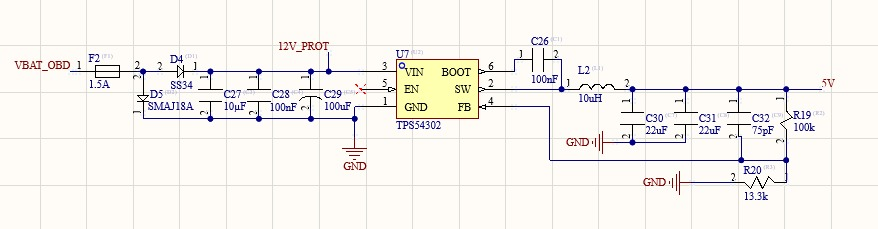
\includegraphics[width=1.02\textwidth]{Images/regu.png}
	
	\vspace{2mm}
	\small\raggedright
	\textit{Nota.} Diagrama eléctrico de la etapa de potencia regulada tipo reductora (\textit{Buck}) basada en el controlador TPS54302. Incluye las etapas de protección de entrada (fusible PTC rearmable, diodo Schottky de protección contra inversión de polaridad y diodo TVS), el filtro de potencia LC y el lazo de realimentación ajustado para una salida estable de 5~V/3~A.
\end{figure}

\begin{figure}[H]
	% Formato APA 7 con protección para el índice de figuras
	\captionsetup{labelformat=simple, labelsep=newline, textfont=it, labelfont=bf, justification=raggedright, singlelinecheck=false}
	\caption[Esquemático de los reguladores LDO AMS1117 y AP2112 en Altium Designer]{Esquemático del circuito de regulación lineal para la alimentación de 3.3~V.}
	\label{fig:esquematico_reg_3v3}
	\centering
	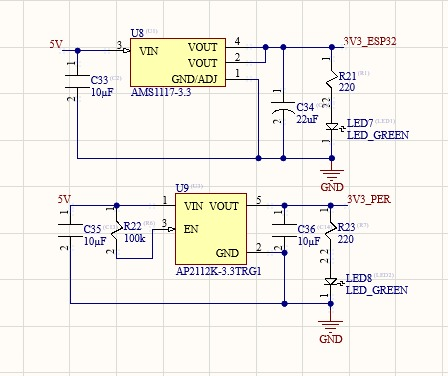
\includegraphics[width=0.8\textwidth]{Images/regum.png} % Modifica el nombre de la imagen si es necesario
	
	\vspace{2mm}
	\small\raggedright
	\textit{Nota.} Diagrama eléctrico de la etapa de regulación lineal que reduce el voltaje de 5~V a 3.3~V. El diseño emplea los reguladores de baja caída de tensión (LDO, por sus siglas en inglés) AMS1117 y AP2112 para suministrar energía de forma estable al microcontrolador y periféricos de 3.3~V. 
\end{figure}

\subsubsection{Sistema transceptor CAN}

Para la comunicación en el bus CAN, se seleccionó el transceptor SN65HVD230 (ver Tabla \ref{tab:componentes_seleccionados}). La configuración del circuito se realizó siguiendo las recomendaciones técnicas detalladas en su hoja de datos \citep{sn65hvd230_datasheet}, la cual describe la implementación óptima para garantizar la integridad de la señal. La configuración del esquema de conexión se ilustra en la Figura \ref{fig:sn65}

\begin{figure}[H]
	% Se usa labelformat=simple para que LaTeX gestione la numeración automáticamente
	\captionsetup{labelformat=simple, labelsep=period, textfont=it, labelfont=bf, justification=raggedright, singlelinecheck=false}
	
	\caption{Configuración de conexión óptima del transceptor CAN SN65HVD230}
	\label{fig:sn65}
	
	\vspace{4mm}
	% Imagen de la conexión del transceptor
	\centering
	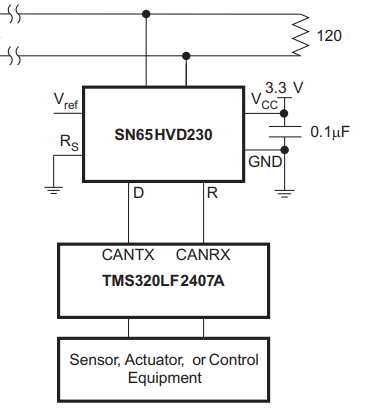
\includegraphics[width=0.40\textwidth]{Images/sn65.png}
	
	\vspace{4mm}
	% Nota a la izquierda
	\raggedright
	\small
	\textit{Nota.} Diagrama de conexión típica para el transceptor SN65HVD230, incluyendo la resistencia de terminación de 120 $\Omega$ entre las líneas CANH y CANL para evitar reflexiones en el bus, y la configuración de los pines de control para el modo de operación de alta velocidad. Adaptado de \citet{sn65hvd230_datasheet}.
\end{figure}

Tras analizar el esquema de los módulos basados en el SN65HVD230, se identificó una resistencia adicional conectada al pin RS (Rate Select). Asimismo, se añadió un PediScan, cuya función es actuar como un escáner y herramienta de diagnóstico automotriz, permitiendo la comunicación con la ECU del vehículo a través del puerto OBD-II para la lectura de parámetros, códigos de diagnóstico (DTC) y datos en tiempo real. Su incorporación permitió tomar como referencia un dispositivo comercial ampliamente utilizado para validar el diseño de la interfaz CAN implementada. Al integrar esta configuración en el diseño, el sistema resultante se ilustra en la Figura \ref{fig:esquema_can}.

\begin{figure}[H]
	% Formato APA 7 con protección para el índice de figuras
	\captionsetup{labelformat=simple, labelsep=newline, textfont=it, labelfont=bf, justification=raggedright, singlelinecheck=false}
	\caption[Esquemático del transceptor CAN SN65HVD230 en EasyEDA]{Esquemático del circuito transceptor CAN basado en el SN65HVD230.}
	\label{fig:esquema_can}
	\centering
	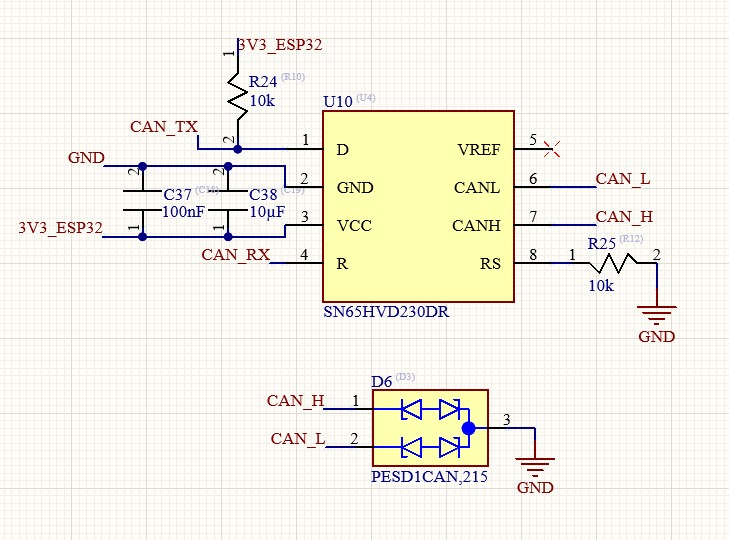
\includegraphics[width=0.9\textwidth]{Images/esquematico_can_final.png}
	
	\vspace{2mm}
	\small\raggedright
	\textit{Nota.} Diagrama eléctrico de la interfaz de comunicación CAN basada en el transceptor SN65HVD230. Incluye la configuración de los pines de control, la red de desacoplamiento de alimentación y la resistencia de terminación de 120 $\Omega$ necesaria para la integridad del bus, siguiendo las especificaciones de diseño recomendadas en la hoja de datos del fabricante.
\end{figure}


\subsubsection{Sistema de procesamiento}

Para este sistema se optó por el módulo \textbf{ESP32-S3-WROOM-1-N16R8}, el cual integra el microcontrolador ESP32-S3 de Espressif Systems. Este dispositivo incorpora un procesador de doble núcleo basado en la arquitectura Xtensa\textsuperscript{\textregistered} LX7 de hasta 240 MHz, conectividad Wi-Fi de 2.4 GHz y Bluetooth Low Energy (BLE) 5.0, además de una memoria Flash integrada de 16 MB y 8 MB de PSRAM. Estas características proporcionan la capacidad de ejecutar simultáneamente las tareas de adquisición de datos del vehículo, almacenamiento en memoria microSD, comunicación mediante el protocolo CAN y la implementación de un servidor web local para la visualización de información en tiempo real; el desempeño del sistema se mantiene estable incluso con estas tareas corriendo en paralelo \citep{espressif_esp32_datasheet}. Para asegurar el correcto funcionamiento del microcontrolador se debe implementar, además, la configuración mínima de hardware recomendada por el fabricante, tal como se ilustra en la Figura \ref{fig:conexion_minima_esp32}.

\begin{figure}[H]
	% Formato APA 7 con numeración automática gestionada por LaTeX
	\captionsetup{labelformat=simple, labelsep=newline, textfont=it, labelfont=bf, justification=raggedright, singlelinecheck=false}
	
	\caption{Circuito de conexión mínima y configuración óptima del módulo ESP32-S3-WROOM-1-N16R8.}
	\label{fig:conexion_minima_esp32}
	\centering
	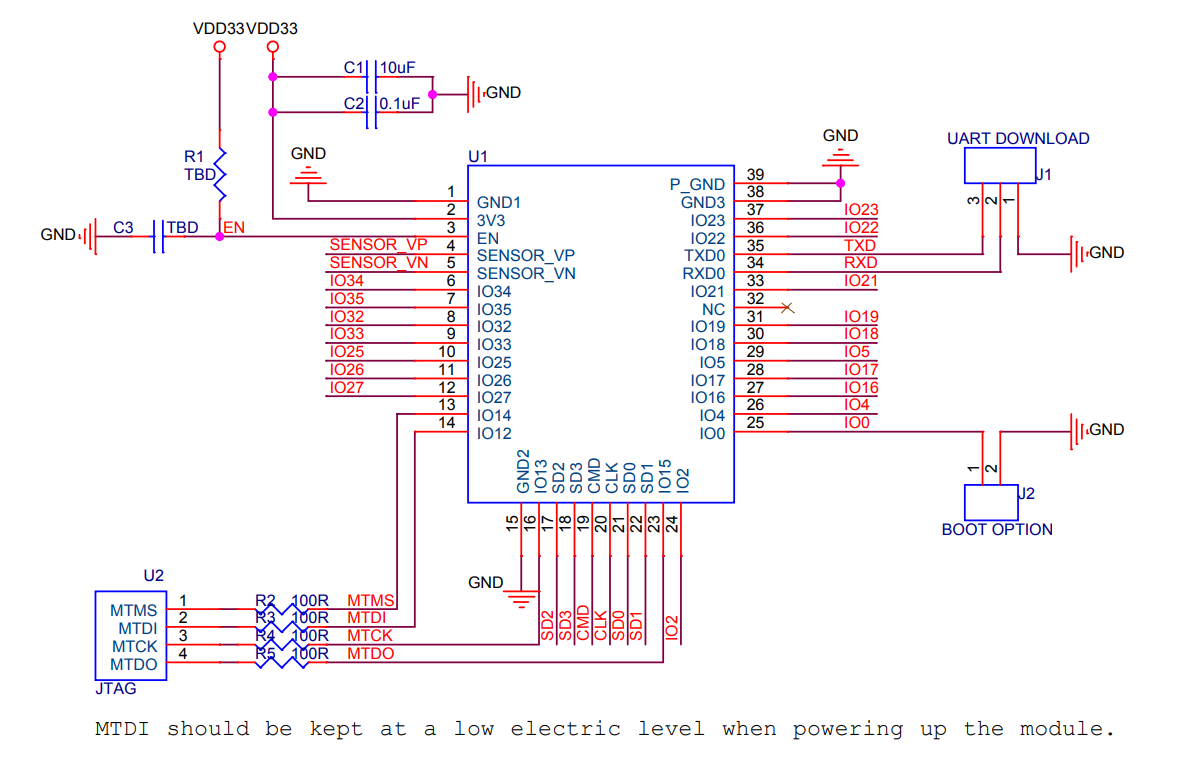
\includegraphics[width=1.02\textwidth]{Images/esp32_conexion_optima.png}
	
	\vspace{2mm}
	\small\raggedright
	\textit{Nota.} Esquemático de la configuración de hardware requerida para el correcto funcionamiento del módulo ESP32-S3-WROOM-1-N16R8. Se muestra el circuito de habilitación y reinicio mediante el pin EN, los condensadores de desacoplamiento de la alimentación de 3.3 V ubicados próximos al módulo, así como la configuración recomendada de los pines de arranque y programación para garantizar una inicialización estable del sistema. Adaptado de \textit{ESP32-S3-WROOM-1 Datasheet}, por Espressif Systems, 2024.
\end{figure}

La integración definitiva de la etapa de procesamiento se consolidó mediante el diseño del circuito impreso en la plataforma Altium Designer. Este esquema incorpora las recomendaciones establecidas por el fabricante para el módulo ESP32-S3-WROOM-1-N16R8 y la integración de los diferentes periféricos empleados en el sistema, optimizando la distribución de las señales de alimentación, comunicación y control para mejorar la estabilidad eléctrica y el rendimiento general del dispositivo. El resultado de esta integración y la topología eléctrica final del sistema basado en el microcontrolador se presentan detalladamente en la Figura \ref{fig:esp32fin}.

\begin{figure}[H]
	% Formato APA 7 con protección para el índice de figuras
	\captionsetup{labelformat=simple, labelsep=newline, textfont=it, labelfont=bf, justification=raggedright, singlelinecheck=false}
	\caption[Esquemático final del módulo ESP32-S3-WROOM-1-N16R8 en EasyEDA]{Esquemático completo del circuito de control y periféricos basados en el ESP32-S3-WROOM-1-N16R8.}
	\label{fig:esp32fin}
	\centering
	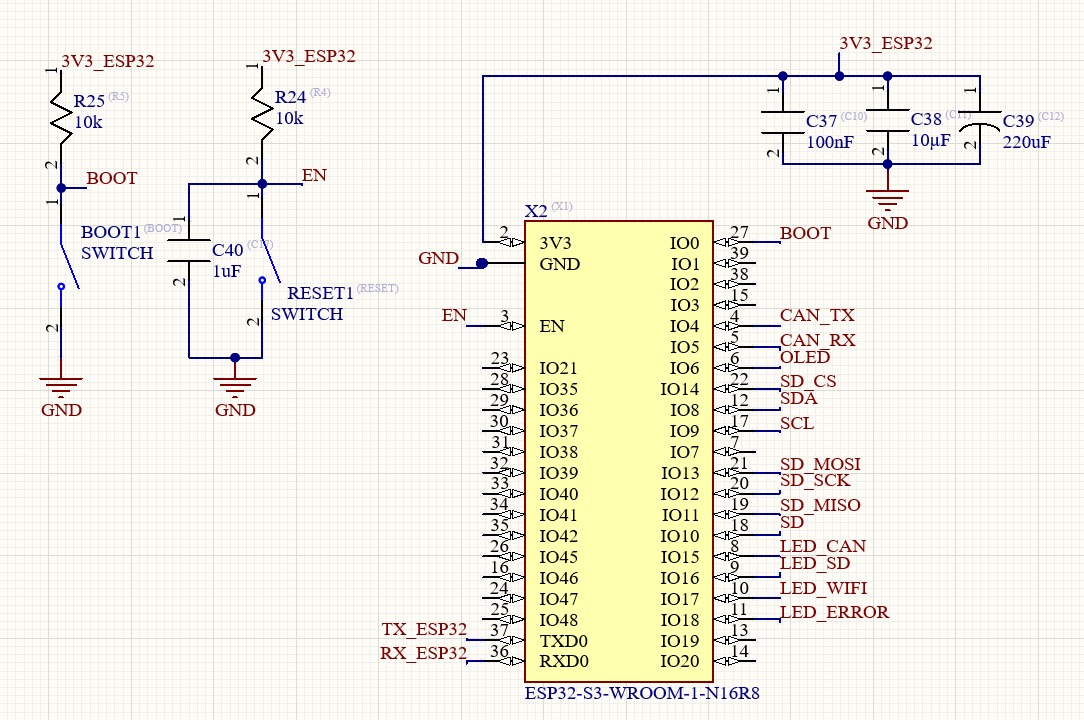
\includegraphics[width=1.02\textwidth]{Images/ESP32_FINAL.png}
	
	\vspace{2mm}
	\small\raggedright
	\textit{Nota.} Diagrama eléctrico final desarrollado en Altium Designer para la etapa de procesamiento basada en el módulo ESP32-S3-WROOM-1-N16R8. El diseño integra las recomendaciones de la hoja de datos del fabricante, el acondicionamiento de la alimentación, el circuito de programación y reinicio automático, así como la conexión de los periféricos utilizados en el sistema para garantizar un funcionamiento confiable durante la adquisición, procesamiento y visualización de los datos obtenidos desde el puerto OBD-II.
\end{figure}


\subsubsection{Sistema de visualización}

Una vez definida la distribución de señales del conector de expansión, se procedió al diseño del esquemático de la etapa de visualización utilizando el software Altium Designer. En este diseño se integran la pantalla OLED, el conector JST-GH, las resistencias \textit{pull-up} del bus $I^2C$ y el condensador de desacoplamiento, obteniéndose el circuito mostrado en la Figura \ref{fig:esquematico_visualizacion}.

\begin{table}[H]
	\centering
	\captionsetup{labelformat=simple, labelsep=newline, textfont=it, labelfont=bf, justification=raggedright, singlelinecheck=false}
	\caption{Asignación de pines y código de colores del conector de expansión de 6 pines}
	\label{tab:pinout_conector}
	\small
	\renewcommand{\arraystretch}{1.3}
	% Mantenemos la calibración exacta de anchos fijos (3.5cm + 2.0cm + 8.7cm = 14.2cm)
	\begin{tabular}{p{3.5cm} p{2.0cm} p{8.7cm}}
		\toprule
		\rowcolor[rgb]{0.851, 0.851, 0.851}
		\textbf{Pin / Función} & \textbf{Color} & \textbf{Descripción} \\
		\midrule
		\texttt{VCC} & Rojo & Alimentación principal del módulo externo regulada a 3{,}3~V. \\
		\texttt{GND} & Negro & Referencia común de tierra del sistema. \\
		\texttt{SCL} & Verde & Línea de reloj de la interfaz de comunicación serial $I^2C$. \\
		\texttt{SDA} & Azul & Línea de datos bidireccional de la interfaz de comunicación serial $I^2C$. \\
		\bottomrule
	\end{tabular}
	\vspace{0.2cm}
	\begin{flushleft}
		\small
		\begin{center}
			\textit{Nota.} La distribución de señales del conector de expansión garantiza la compatibilidad con sensores periféricos a través del bus de comunicación $I^2C$. Las líneas auxiliares permiten la integración posterior de interrupciones de hardware o señales de control adicionales sin necesidad de modificar el diseño base del circuito impreso.
		\end{center}
	\end{flushleft}
\end{table}

Definida el uso de este conector se procede a dibujar el esquemático (ver Figura \ref{fig:esquematico_visualizacion}) donde su conexión sera al oled.

\begin{figure}[H]
	% Formato APA 7 con protección para el índice de figuras (Mismo estilo de tus otras figuras de EasyEDA)
	\captionsetup{labelformat=simple, labelsep=newline, textfont=it, labelfont=bf, justification=raggedright, singlelinecheck=false}
	\caption[Esquemático de la etapa de visualización OLED en EasyEDA]{Esquemático del circuito de visualización física y conector de expansión periférico.}
	\label{fig:esquematico_visualizacion}
	\centering
	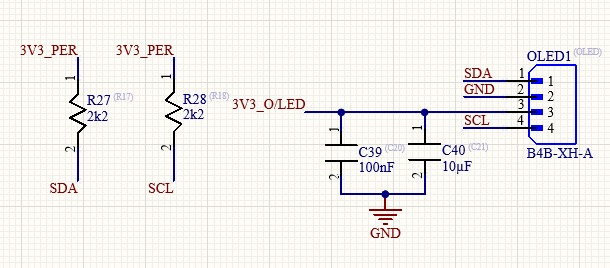
\includegraphics[width=0.9\textwidth]{Images/visu.png}
	
	\vspace{2mm}
	\small\raggedright
	\textit{Nota.} \textit{Nota.} Diagrama esquemático desarrollado en Altium Designer para la etapa de visualización del sistema. El diseño incorpora la pantalla OLED, el conector JST-GH de seis pines para su conexión externa, las resistencias \textit{pull-up} de las líneas SDA y SCL del bus $I^2C$, así como el condensador de desacoplamiento de 100~nF ubicado próximo al periférico para mejorar la estabilidad de la alimentación y la integridad de la comunicación en aplicaciones con cableado de mayor longitud..
\end{figure}

\subsubsection{Sistema de almacenamiento de datos}

Con el propósito de almacenar de forma local los datos obtenidos desde el sistema OBD-II, se incorporó una memoria MicroSD al diseño electrónico. Su utilización permite registrar de manera permanente las variables adquiridas por el ESP32-S3-WROOM-1-N16R8, facilitando el almacenamiento de grandes volúmenes de información para su posterior análisis sin depender de una conexión inalámbrica o de un servidor externo. Esta característica resulta especialmente útil durante las pruebas de campo, donde es necesario conservar el historial completo de los parámetros del vehículo para realizar comparaciones, validar modelos matemáticos y analizar el comportamiento del sistema en diferentes condiciones de operación.

La implementación de esta etapa se basó en las especificaciones de la SD Card Association \citep{transcend_microsd_datasheet}. Debido a que tanto el módulo ESP32-S3-WROOM-1-N16R8 como las tarjetas MicroSD operan con niveles lógicos de 3.3 V, fue posible realizar la conexión directa entre ambos dispositivos sin necesidad de incorporar convertidores de nivel lógico, simplificando el diseño y reduciendo el número de componentes.

Para la comunicación entre el microcontrolador y la memoria se seleccionó el protocolo SPI (Serial Peripheral Interface), debido a su elevada velocidad de transferencia, simplicidad de implementación y reducido número de líneas de comunicación. En esta configuración se emplean las señales SCK, MOSI, MISO y CS para gestionar el acceso a la memoria durante las operaciones de lectura y escritura.

Con el objetivo de garantizar un funcionamiento confiable del sistema, se incorporaron condensadores de desacoplamiento de 10~$\mu$F y 100~nF próximos al conector MicroSD. El condensador de 10~$\mu$F proporciona una reserva de energía para compensar los picos de corriente que se presentan durante las operaciones de escritura, mientras que el condensador cerámico de 100~nF filtra las componentes de alta frecuencia presentes en la alimentación, reduciendo el ruido eléctrico y mejorando la estabilidad del sistema.

También se implementaron resistencias de 10~k$\Omega$ conectadas a las líneas DAT1, DAT2 y DAT3/CS de la tarjeta MicroSD. Estas resistencias mantienen dichas líneas en un nivel lógico alto cuando no están siendo utilizadas, evitando estados flotantes durante el encendido del sistema, la inserción o extracción de la tarjeta y mejorando la confiabilidad del proceso de inicialización, de acuerdo con las recomendaciones de diseño para dispositivos compatibles con tarjetas SD. El esquema eléctrico final de esta etapa se presenta en la Figura \ref{fig:esquematico_microsd}.

\begin{figure}[H]
	\captionsetup{labelformat=simple, labelsep=newline, textfont=it, labelfont=bf, justification=raggedright, singlelinecheck=false}
	\caption[Esquemático del sistema de almacenamiento mediante memoria MicroSD en Altium Designer]{Esquemático de la etapa de almacenamiento de datos mediante tarjeta MicroSD.}
	\label{fig:esquematico_microsd}
	\centering
	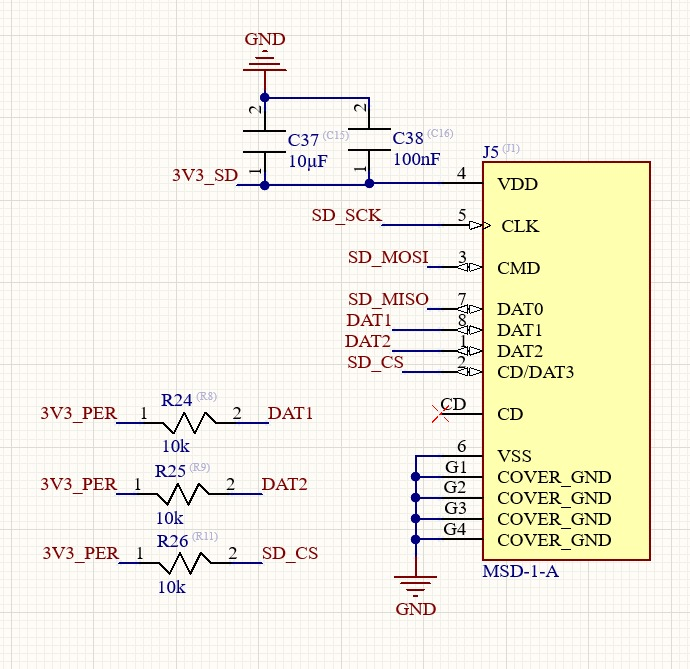
\includegraphics[width=0.75\textwidth]{Images/sd.png}
	
	\vspace{2mm}
	\small\raggedright
	\textit{Nota.} Diagrama esquemático desarrollado en Altium Designer para la interfaz de almacenamiento mediante memoria MicroSD. El diseño incorpora los condensadores de desacoplamiento de 10~$\mu$F y 100~nF para estabilizar la alimentación durante las operaciones de lectura y escritura, así como resistencias de 10~k$\Omega$ conectadas a las líneas DAT1, DAT2 y DAT3/CS, las cuales mantienen dichas señales en un estado lógico definido durante el arranque e inicialización de la tarjeta, incrementando la confiabilidad de la comunicación SPI con el módulo ESP32-S3-WROOM-1-N16R8.
\end{figure}

\subsubsection{Sistema de programación de uso de periféricos}

\subsubsection{Control de alimentación de periféricos}

Con el propósito de optimizar el consumo energético del sistema y permitir una administración independiente de los dispositivos auxiliares, se incorporó un interruptor electrónico de carga TPS22918. Este circuito integrado permite conectar o desconectar la alimentación de los periféricos mediante una señal de control proveniente del microcontrolador ESP32-S3-WROOM-1-N16R8.

En el diseño propuesto, dos pines GPIO del ESP32-S3 controlan el estado lógico de habilitación del TPS22918, permitiendo energizar únicamente los dispositivos cuando son requeridos por la aplicación. Los principales periféricos alimentados mediante este circuito son la memoria MicroSD y la pantalla OLED, los cuales permanecen desenergizados durante el proceso de inicialización del sistema o cuando no se encuentran en uso; así se reduce el consumo de corriente y se evitan inicializaciones indeseadas.

La utilización del TPS22918 también proporciona un encendido controlado de los periféricos gracias a su baja resistencia de conducción (\textit{R\textsubscript{ON}}) y a su mecanismo interno de control de la corriente de irrupción (\textit{Inrush Current}) (ver Apéndice L), evitando caídas bruscas de tensión sobre la línea de alimentación de 3.3 V durante la conexión de cargas capacitivas. Estas características contribuyen a mejorar la estabilidad del sistema y la confiabilidad del funcionamiento del microcontrolador durante el arranque y la operación normal.

El esquemático correspondiente a la etapa de control de alimentación se presenta en la Figura \ref{fig:esquematico_programacion}.

\begin{figure}[H]
	\captionsetup{labelformat=simple, labelsep=newline, textfont=it, labelfont=bf, justification=raggedright, singlelinecheck=false}
	\caption[Esquemático del control de alimentación de periféricos]{Esquemático de la etapa de control de alimentación mediante el interruptor electrónico TPS22918.}
	\label{fig:esquematico_programacion}
	\centering
	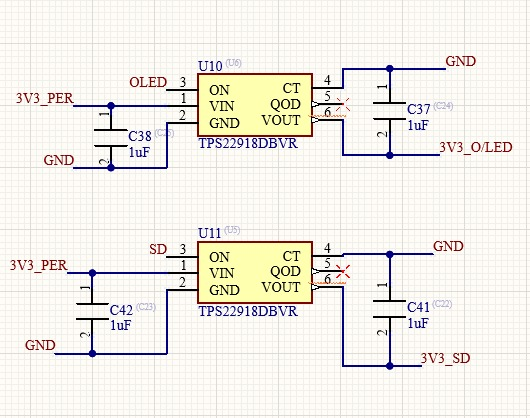
\includegraphics[width=0.82\textwidth]{Images/PROGRAMACION.png}
	
	\vspace{2mm}
	\small\raggedright
	\textit{Nota.} Diagrama esquemático desarrollado en Altium Designer para el control de alimentación de los periféricos del sistema. El circuito emplea un interruptor electrónico TPS22918, controlado mediante señales GPIO del módulo ESP32-S3-WROOM-1-N16R8, para habilitar o deshabilitar la alimentación de la memoria MicroSD y la pantalla OLED. Esta estrategia permite reducir el consumo energético, controlar la secuencia de encendido de los periféricos y mejorar la estabilidad de la línea de alimentación de 3.3 V al limitar la corriente de irrupción durante la conexión de las cargas.
\end{figure}

\subsubsection{Sistema de monitoreo y estado}

\subsubsection{Indicadores de estado}

Con el propósito de facilitar el diagnóstico visual y el monitoreo del estado operativo del sistema, se incorporó un conjunto de indicadores luminosos basados en diodos emisores de luz (LED) de montaje superficial (SMD). Estos indicadores permiten conocer de forma inmediata el estado de los principales módulos del dispositivo durante su funcionamiento: las tareas de depuración, mantenimiento y validación del sistema pueden hacerse así sin herramientas externas de diagnóstico.

Cada LED es controlado mediante un pin de propósito general (GPIO) del módulo ESP32-S3-WROOM-1-N16R8, permitiendo que el firmware indique diferentes estados de operación de acuerdo con los eventos generados por el sistema. Para limitar la corriente que circula por cada diodo y proteger tanto los LED como las salidas digitales del microcontrolador, se incorporó una resistencia de 220~$\Omega$ conectada en serie con cada indicador.

El sistema de señalización está conformado por los siguientes indicadores:

\begin{itemize}
	\item \textbf{LED CAN (morado):} Indica la actividad de comunicación sobre el bus CAN, encendiéndose o parpadeando durante la transmisión y recepción de tramas provenientes de la ECU del vehículo.
	
	\item \textbf{LED MicroSD (naranja):} Señaliza las operaciones de acceso a la memoria MicroSD, incluyendo procesos de inicialización, lectura y escritura de archivos de registro.
	
	\item \textbf{LED ERROR (rojo):} Indica la presencia de fallas detectadas por el sistema, como errores de comunicación, problemas durante la inicialización de los periféricos o cualquier condición anómala registrada por el firmware.
	
	\item \textbf{LED Wi-Fi (azul):} Muestra el estado de la conectividad inalámbrica y del servidor web local implementado en el ESP32-S3, indicando la disponibilidad del sistema para la visualización de datos mediante un navegador web.
\end{itemize}

El esquemático correspondiente a esta etapa se desarrolló en Altium Designer y se presenta en la Figura \ref{fig:esquematico_indicadores}.

\begin{figure}[H]
	\captionsetup{labelformat=simple, labelsep=newline, textfont=it, labelfont=bf, justification=raggedright, singlelinecheck=false}
	\caption[Esquemático del sistema de indicadores visuales]{Esquemático del circuito de indicadores LED para el monitoreo del estado del sistema.}
	\label{fig:esquematico_indicadores}
	\centering
	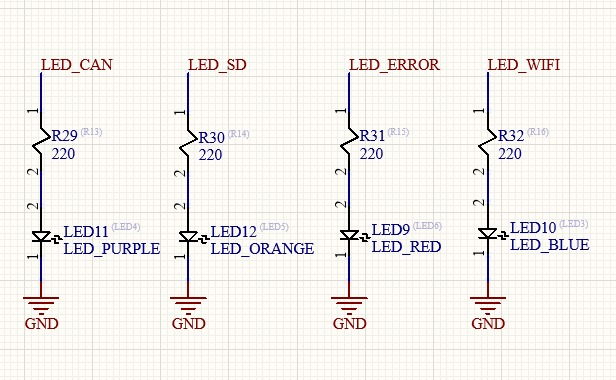
\includegraphics[width=0.82\textwidth]{Images/INDICADOR.png}
	
	\vspace{2mm}
	\small\raggedright
	\textit{Nota.} Diagrama esquemático desarrollado en Altium Designer para el sistema de indicadores visuales. Cada LED se encuentra conectado a un GPIO del módulo ESP32-S3-WROOM-1-N16R8 mediante una resistencia limitadora de 220~$\Omega$, la cual restringe la corriente que circula por el diodo, protege las salidas digitales del microcontrolador y prolonga la vida útil de los indicadores. Los cuatro LED permiten visualizar el estado de la comunicación CAN, la actividad de la memoria MicroSD, la conectividad Wi-Fi y la presencia de condiciones de error detectadas durante el funcionamiento del sistema.
\end{figure}

\subsection{Placa preliminar (EasyEDA)}
\label{sec:pcb_preliminar_diseno}

Antes de proceder con el diseño de la placa final descrito en el resto de esta sección, se desarrolló en EasyEDA una placa preliminar que replica el mismo circuito ya validado sobre protoboard (Capítulo~4, Sección~4.1.3), con el fin de contar con una versión física más robusta que las conexiones sueltas de una protoboard para las pruebas de campo. A diferencia de la placa final, esta versión preliminar resuelve la alimentación con un regulador lineal simple (7805 más un transistor de paso TIP42C en configuración de refuerzo de corriente) en lugar de la conversión conmutada de dos rieles, y conecta el transceptor CAN, la pantalla OLED y el módulo microSD --ya validados en la etapa de protoboard-- mediante conectores de pines en vez de integrarlos directamente en la placa. El esquemático completo se muestra en la Figura~\ref{fig:esquematico_pcb_preliminar}.

\begin{figure}[H]
	\captionsetup{labelformat=simple, labelsep=newline, textfont=it, labelfont=bf, justification=raggedright, singlelinecheck=false}
	\caption[Esquemático de la placa preliminar en EasyEDA]{Esquemático completo de la placa preliminar.}
	\label{fig:esquematico_pcb_preliminar}
	\centering
	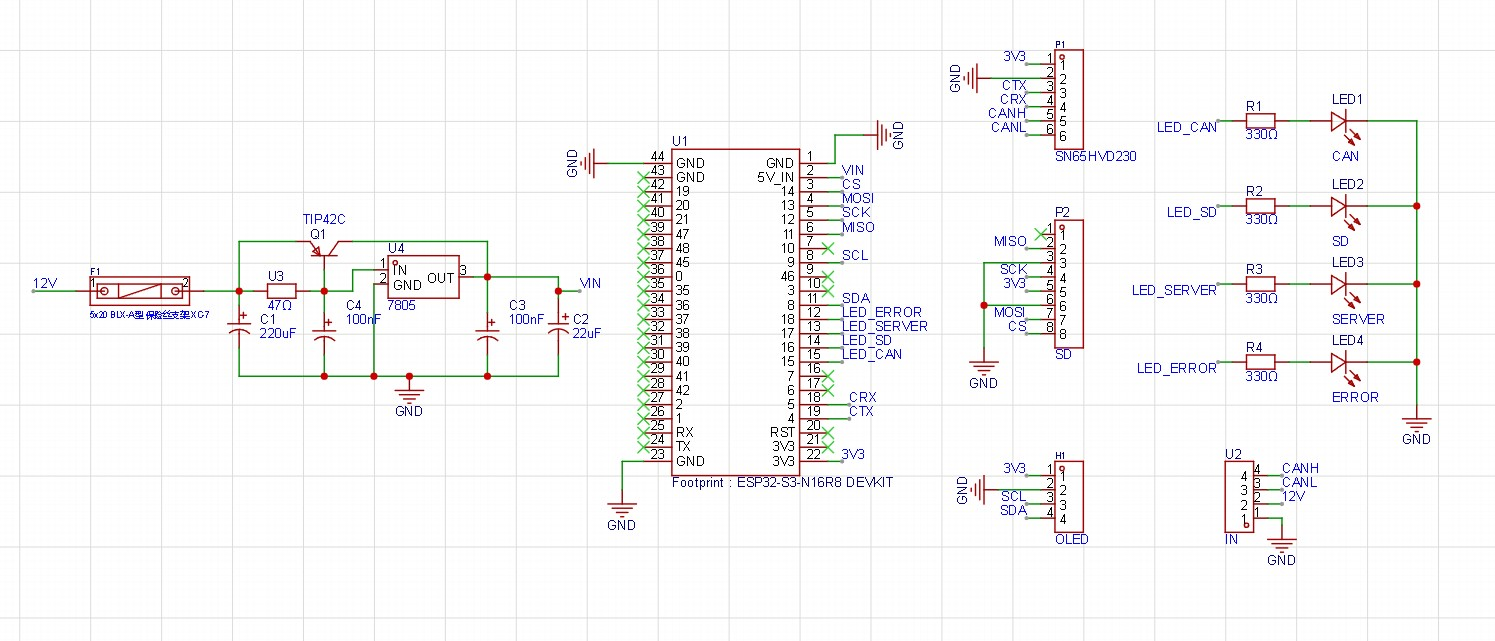
\includegraphics[width=0.95\textwidth]{Images/esquematico_pcb_proto.jpg}

	\vspace{2mm}
	\small\raggedright
	\textit{Nota.} Desarrollado en EasyEDA. El costo detallado de cada componente se presenta en el Capítulo~5 (Tabla~\ref{tab:costo_placa_preliminar_bom}).
\end{figure}

La Figura~\ref{fig:simulacion_pcb_preliminar} muestra la vista 3D generada por EasyEDA a partir de ese esquemático y del enrutado de la placa, previo al envío a fabricar.

\begin{figure}[H]
	\captionsetup{labelformat=simple, labelsep=newline, textfont=it, labelfont=bf, justification=raggedright, singlelinecheck=false}
	\caption[Vista 3D de la placa preliminar en EasyEDA]{Simulación 3D de la placa preliminar, generada en EasyEDA antes de la fabricación.}
	\label{fig:simulacion_pcb_preliminar}
	\centering
	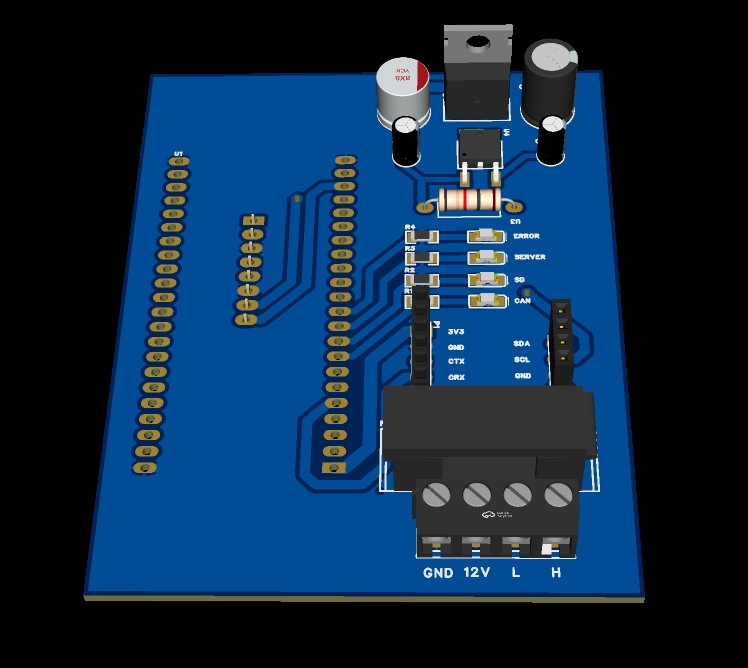
\includegraphics[width=0.55\textwidth]{Images/simulacion_pcb_proto.jpg}
\end{figure}

La fabricación de la placa preliminar se encargó a Robokit (La Paz); la Figura~\ref{fig:fisica_pcb_preliminar} muestra las caras superior e inferior de la placa recibida, previo al ensamblaje de los componentes.

\begin{figure}[H]
	\centering
	\caption{Placa preliminar fabricada por Robokit, sin ensamblar}
	\label{fig:fisica_pcb_preliminar}
	\begin{subfigure}[t]{0.48\textwidth}
		\centering
		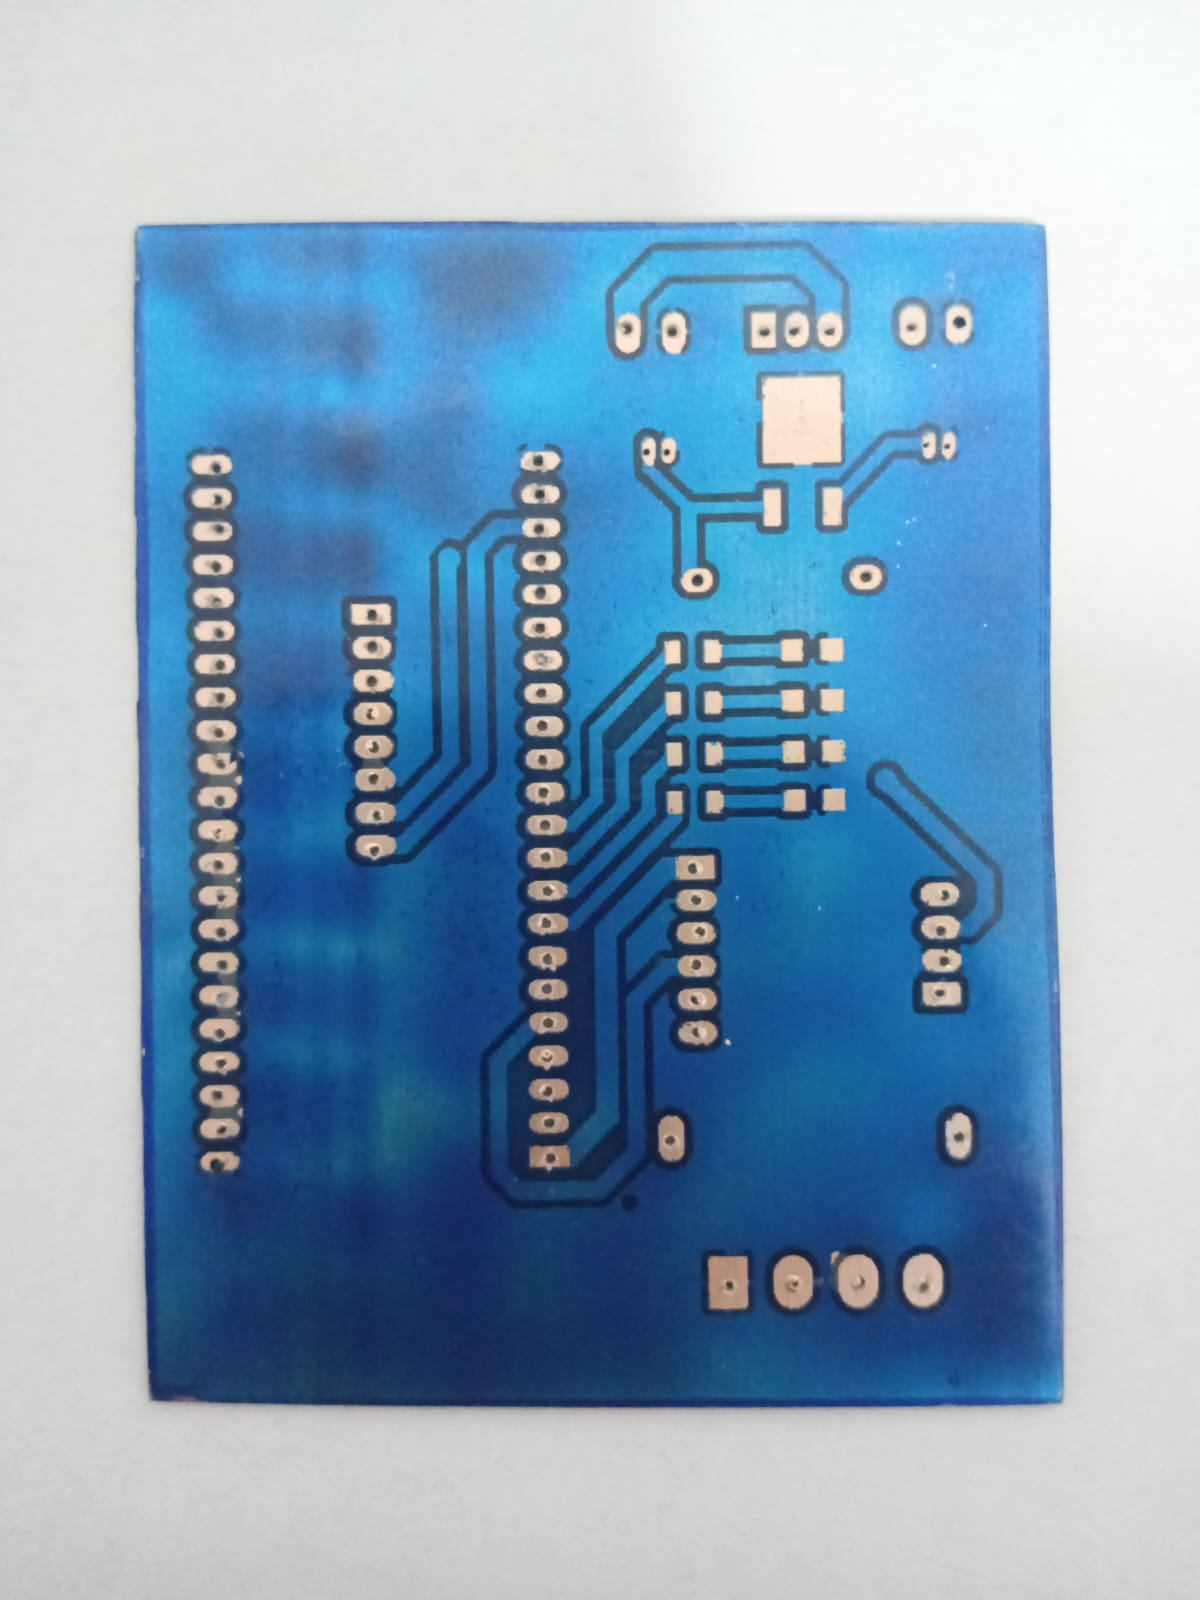
\includegraphics[width=\textwidth]{Images/top_pcb_proto.jpeg}
		\caption{Cara superior (\textit{top})}
		\label{fig:top_pcb_preliminar}
	\end{subfigure}
	\hfill
	\begin{subfigure}[t]{0.48\textwidth}
		\centering
		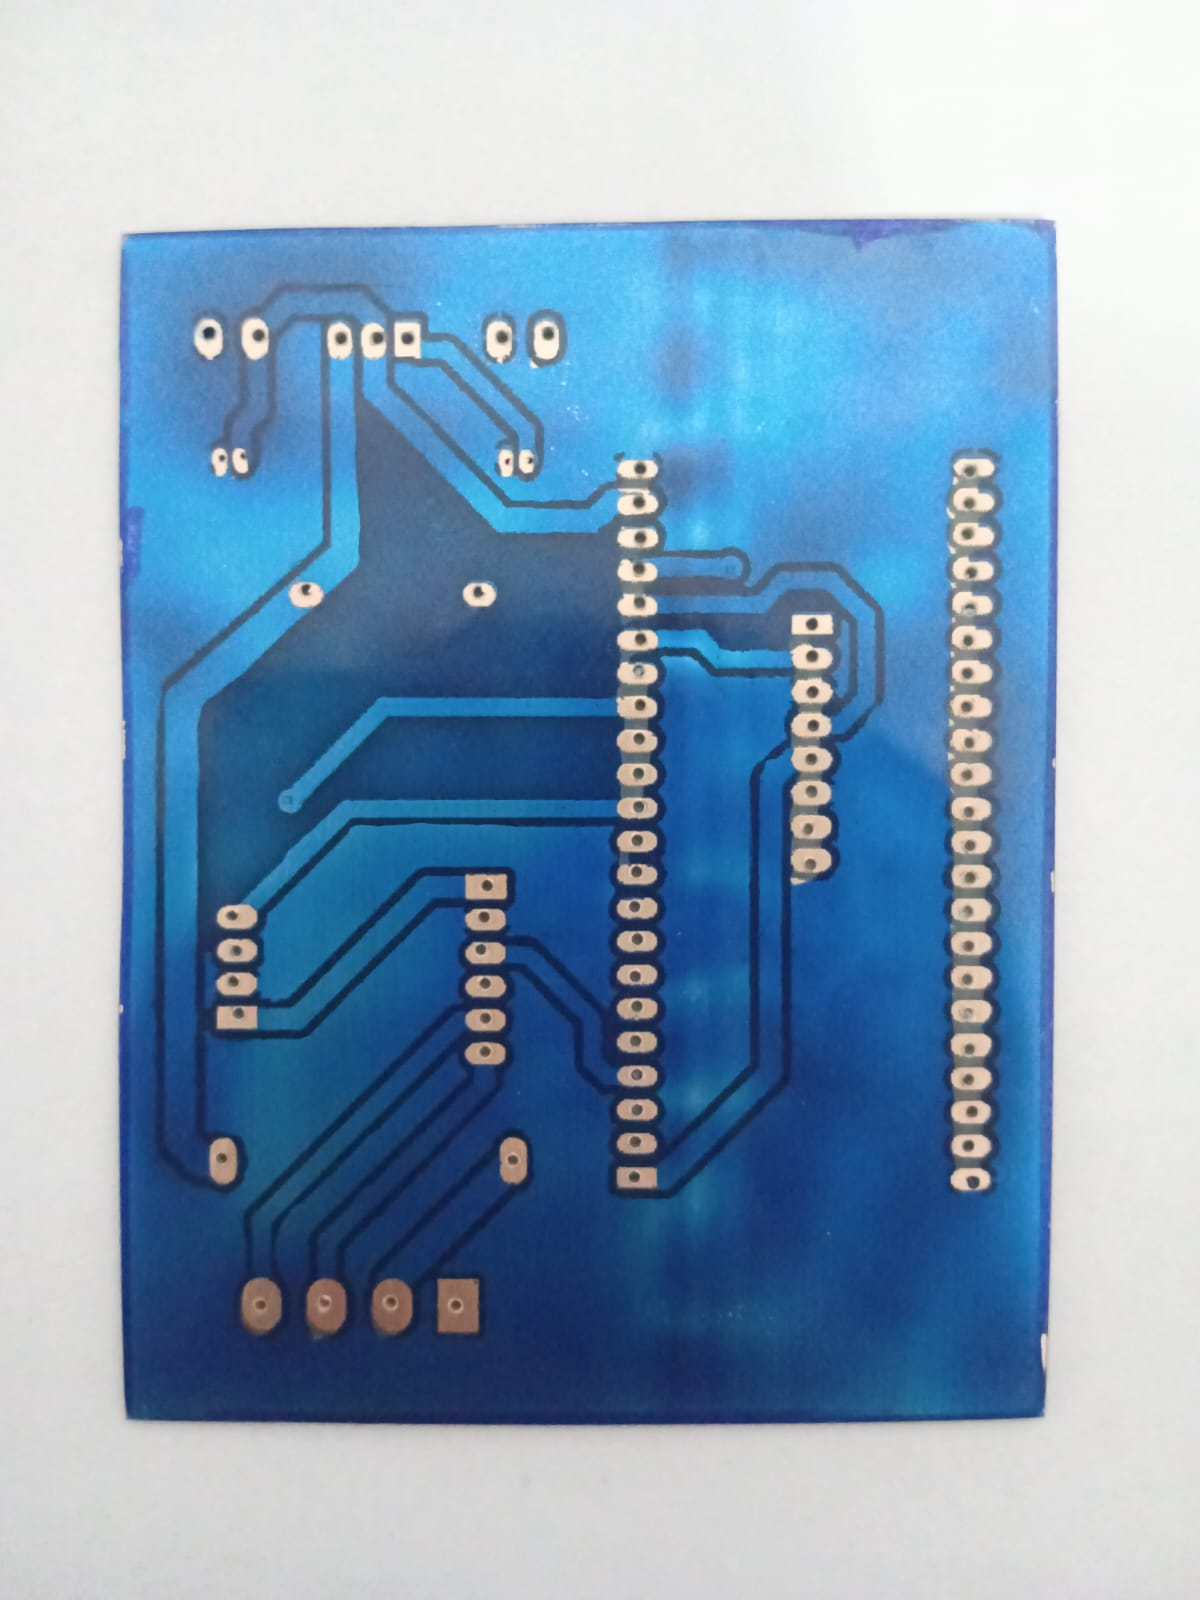
\includegraphics[width=\textwidth]{Images/bottom_pcb_proto.jpeg}
		\caption{Cara inferior (\textit{bottom})}
		\label{fig:bottom_pcb_preliminar}
	\end{subfigure}
	\vspace{2pt}
	\\
	{\footnotesize\textit{Nota.} Placa de una sola cara fabricada por Robokit (La Paz), 150\,Bs (Capítulo~5, Tabla~\ref{tab:costo_pcb_preliminar}); el ensamblaje de los componentes se realizó manualmente. Elaboración propia.}
\end{figure}

Una vez soldados los componentes de la Tabla~\ref{tab:costo_placa_preliminar_bom} (Capítulo~5) sobre esta placa, y reutilizando el módulo ESP32-S3, el transceptor SN65HVD230 y la pantalla OLED ya validados en protoboard, se obtiene la placa ensamblada de la Figura~\ref{fig:ensamblada_pcb_preliminar}.

\begin{figure}[H]
	\centering
	\caption{Placa preliminar ensamblada}
	\label{fig:ensamblada_pcb_preliminar}
	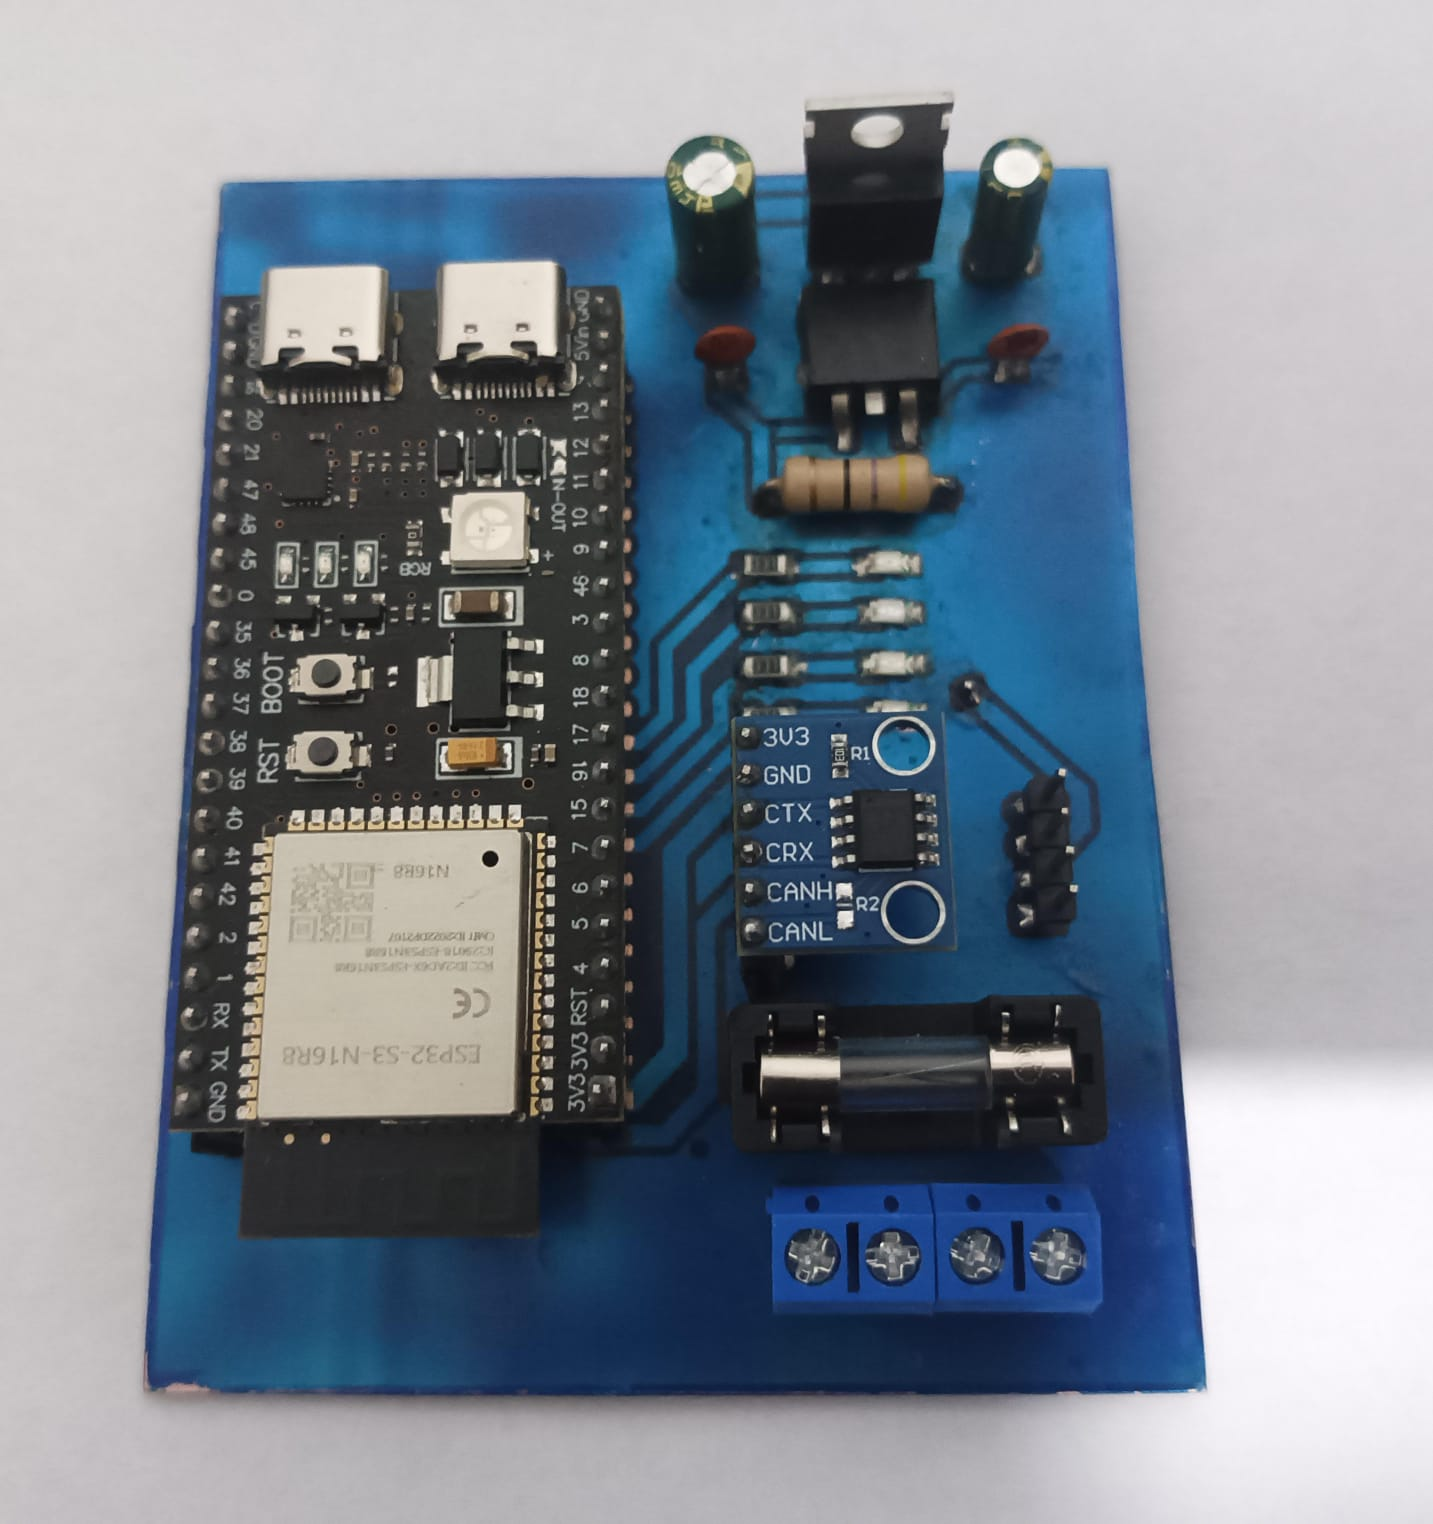
\includegraphics[width=0.6\textwidth]{Images/pcb_proto_ensamblada.jpeg}

	\vspace{2pt}
	{\footnotesize\textit{Nota.} Placa preliminar tras el ensamblaje manual de los componentes: se distinguen el módulo ESP32-S3-N16R8, el regulador 7805 con el transistor de paso TIP42C, el módulo transceptor SN65HVD230 (conectado mediante el header de 6 pines), el fusible reseteable F1 y el conector de entrada de 4 pines (GND, 12~V, CAN\_L, CAN\_H). Elaboración propia.}
\end{figure}

\subsection{Diseño de la carcasa del prototipo (impresión 3D)}
\label{sec:carcasa_prototipo}

Para esta presentación se diseñó e imprimió una carcasa únicamente para la placa preliminar; la carcasa de la placa final queda pendiente y se elaborará si el tribunal la solicita. Como punto de partida se tomó un modelo STL de una caja de dos piezas (base y tapa) publicado en MakerWorld, el repositorio de modelos de Bambu Lab, mostrado en la Figura~\ref{fig:stl_makerworld}.

\begin{figure}[H]
	\centering
	\caption{Modelo STL base, tomado de MakerWorld}
	\label{fig:stl_makerworld}
	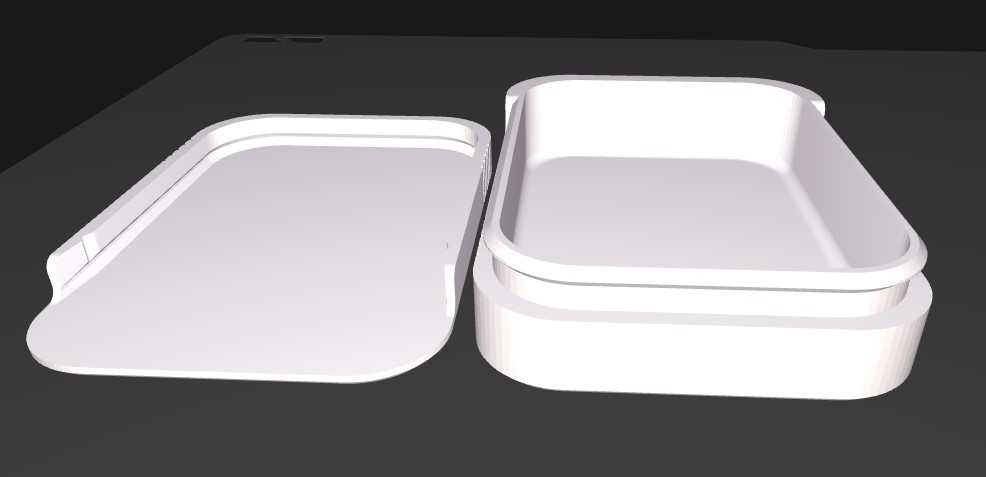
\includegraphics[width=0.7\textwidth]{Images/STL_MAKEWORD.jpg}

	\vspace{2pt}
	{\footnotesize\textit{Nota.} Modelo de caja de dos piezas (base y tapa) publicado en MakerWorld (Bambu Lab), usado como punto de partida antes de la edición en SolidWorks.}
\end{figure}

La tapa del modelo original no contaba con una abertura para la pantalla OLED; se editó en SolidWorks para agregar el recorte rectangular necesario, manteniendo el resto de la geometría del modelo original (Figura~\ref{fig:tapa_editada}).

\begin{figure}[H]
	\centering
	\caption{Tapa modificada en SolidWorks, con abertura para la pantalla OLED}
	\label{fig:tapa_editada}
	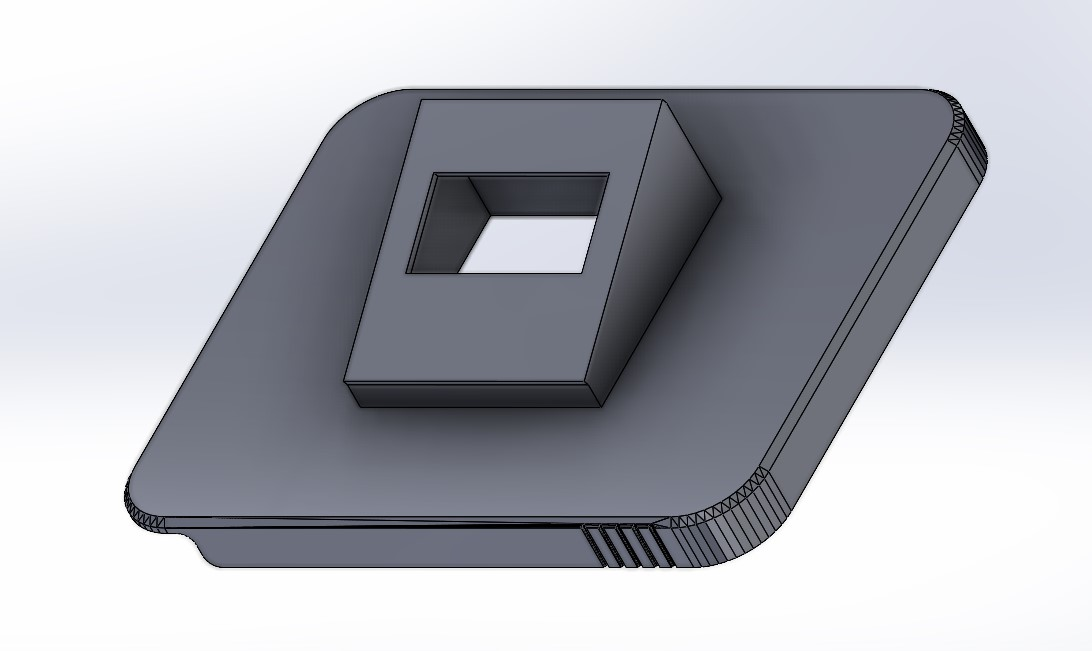
\includegraphics[width=0.6\textwidth]{Images/TAPA_EDITADA.jpg}
\end{figure}

La impresión se realizó en PLA, con una impresora propia Creality Ender V3 KE (Figura~\ref{fig:impresion_3d}). Se eligió PLA en vez de un material más resistente a la intemperie (por ejemplo, PETG o ABS) porque, al tratarse de una carcasa de prototipo, no está expuesta al sol de forma prolongada; esa consideración sí sería relevante para una carcasa de producción instalada de forma permanente en el vehículo.

\begin{figure}[H]
	\centering
	\caption{Impresión 3D en la Creality Ender V3 KE}
	\label{fig:impresion_3d}
	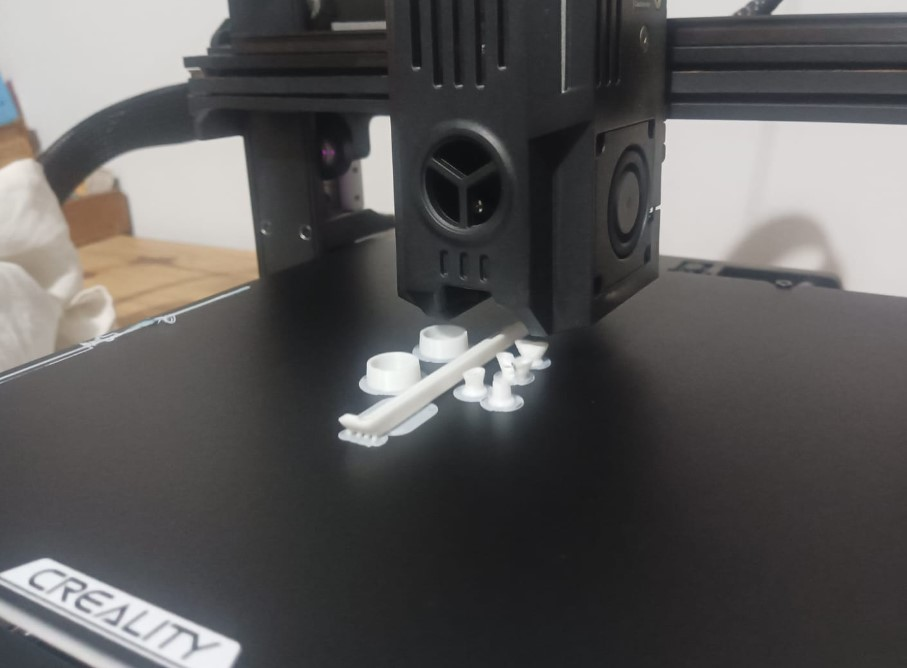
\includegraphics[width=0.7\textwidth]{Images/IMPRESION_3D.jpg}
\end{figure}

La base ya impresa (21~g de PLA) se muestra en la Figura~\ref{fig:carcasa_3d}; la tapa (16~g) está pendiente de impresión al momento de escribir este capítulo. El costo del material se presenta en el Capítulo~5 (Tabla~\ref{tab:costo_carcasa}).

\begin{figure}[H]
	\centering
	\caption{Carcasa impresa del prototipo}
	\label{fig:carcasa_3d}
	\begin{subfigure}[t]{0.48\textwidth}
		\centering
		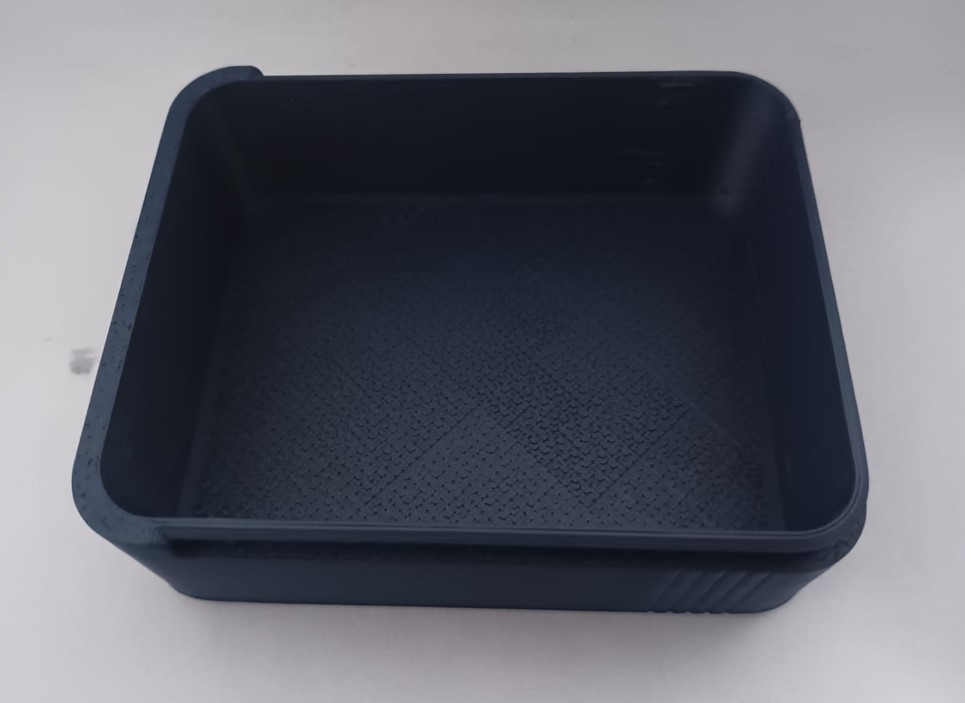
\includegraphics[width=\textwidth]{Images/CARCASA_3D.jpg}
		\caption{Base (impresa, 21~g)}
		\label{fig:carcasa_3d_base}
	\end{subfigure}
	\hfill
	\begin{subfigure}[t]{0.48\textwidth}
		\centering
		\fbox{\parbox[c][0.75\textwidth][c]{\textwidth}{\centering \textit{[Pendiente: fotografía de la tapa una vez impresa]}}}
		\caption{Tapa (pendiente, 16~g)}
		\label{fig:carcasa_3d_tapa}
	\end{subfigure}
	\vspace{2pt}
	\\
	{\footnotesize\textit{Nota.} Impresión propia en PLA. Elaboración propia.}
\end{figure}

\subsection{Diseño de la PCB (Altium Designer)}
% Tu contenido actual: monocapa, anchos de pista, bloques,
% render 3D.
Una vez concluidos los diagramas esquemáticos de cada subsistema, se procedió a la fase de diseño y distribución de la placa de circuito impreso (PCB). Para ello, se utilizó la función 'Import to PCB' integrada en Altium Designer, la cual permite transferir la conectividad lógica y las huellas físicas (footprints) de los componentes. Posteriormente, se realizó la disposición estratégica de los elementos en las diferentes capas (layers) de la placa. En la Figura \ref{fig:pcb} se ilustra detalladamente el proceso de transición de los componentes desde el entorno esquemático hacia el lienzo de diseño definitivo de la PCB. Todos estos documentos tanto como el diagrama esquematico y el layout de la PCB se muestran en el Apendice M

\begin{figure}[H]
	% Formato APA 7 con protección para el índice de figuras (Mismo estilo de tus otras figuras de EasyEDA)
	\captionsetup{labelformat=simple, labelsep=newline, textfont=it, labelfont=bf, justification=raggedright, singlelinecheck=false}
	\caption[Conversión del circuito esquemático al diseño de la PCB en Altium Designer]{Interfaz de transición y mapeo desde el diagrama esquemático hacia el entorno de diseño de la PCB.}
	\label{fig:pcb}
	\centering
	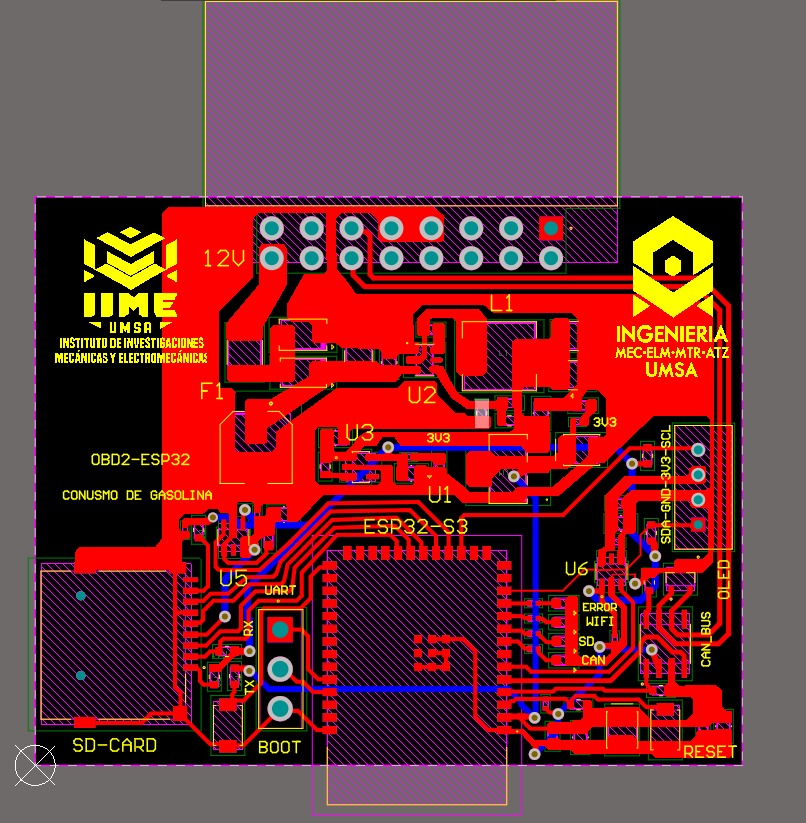
\includegraphics[width=0.85\textwidth]{Images/TRANSICION_PCB.png}
	
	\vspace{2mm}
	\small\raggedright
	\textit{Nota.} Proceso de transferencia y sincronización de componentes mediante la netlist en Altium Designer. Se ilustra cómo los símbolos lógicos del esquema eléctrico se transforman en sus respectivas huellas físicas (footprints) sobre el lienzo bidimensional de la placa de circuito impreso, quedando dispuestos para la organización de capas y el ruteado definitivo de las pistas de cobre.
\end{figure}

Previo a la fase de distribución (layout) y ruteo de las pistas de cobre, es fundamental establecer ciertos criterios técnicos de diseño. Estas consideraciones preliminares permiten optimizar la integridad de las señales, asegurar el manejo correcto de la potencia y garantizar la viabilidad de manufactura de la PCB.

\subsubsection{Criterios de integridad de señal}
% Ancho de pista por corriente (IPC-2221).
% Longitud equivalente CANH/CANL, desacople local VCC.
% Via stitching y plano de tierra (si aplica).
El diseño de circuitos impresos está regulado por estándares internacionales que garantizan su fiabilidad, rendimiento y manufacturabilidad. Entre ellos, la norma IPC-2221 (Generic Standard on Printed Board Design) constituye el pilar fundamental que establece las directrices lógicas y físicas para el desarrollo de PCB. Dentro de las buenas prácticas estipuladas por esta normativa, destacan los siguientes criterios:

\begin{itemize}
	\item \textbf{Sistemas de unidades:} Definir el sistema de medición es un paso preliminar crítico en el desarrollo de la PCB. En la práctica de la ingeniería electrónica, se prioriza el uso del sistema imperial (mils y pulgadas), debido a que el paso (pitch) y la distribución de los pines en la gran mayoría de los componentes y encapsulados comerciales están estandarizados bajo este sistema de medidas.
	
	\item \textbf{Configuración de rejillas (Grids):} La correcta gestión del grid es indispensable para garantizar la precisión geométrica, simetría y alineación del circuito. Un grid de 100~mils constituye el estándar industrial para la distribución de componentes de inserción (Through-Hole), ya que se acopla perfectamente con los centros de perforación. Para el trazo y ruteado de pistas, se adopta de forma general una rejilla de 50~mils, la cual puede reducirse a 25~mils o valores inferiores para diseños de alta densidad que requieran un nivel de detalle más fino.
	
	\item \textbf{Dimensionamiento de pistas:} El ancho de los conductores no está condicionado por un valor absoluto, sino que depende estrictamente de los requerimientos eléctricos del circuito (capacidad de corriente), el espacio disponible para el enrutamiento y las distancias de aislamiento (clearance). En la Tabla \ref{tab:pistas} se presentan los valores geométricos sugeridos; el cálculo matemático para determinar el ancho óptimo en función de la corriente y la elevación térmica es, de por sí, complejo, así que la industria se fundamenta en ecuaciones empíricas y curvas de comportamiento no lineal que han sido recopiladas y validadas experimentalmente por organismos normativos a lo largo de décadas de pruebas de laboratorio.
	
	\begin{table}[H]
		% Formato APA 7 (Estilo homogéneo, limpio y profesional)
		\captionsetup{labelformat=simple, labelsep=newline, textfont=it, labelfont=bf, justification=raggedright, singlelinecheck=false}
		\caption{Ancho de pista recomendado y resistencia estimada en función de la corriente}
		\label{tab:pistas}
		\centering
		\begin{tabular}{cccc}
			\toprule
			\rowcolor[rgb]{0.851, 0.851, 0.851}
			\textbf{Corriente (Amp)} & \textbf{1 oz (mils)} & \textbf{2 oz (mils)} & \textbf{Resistencia (m$\Omega$/plg)} \\
			\midrule
			1  & 10  & 5   & 52,0 \\
			2  & 30  & 15  & 17,2 \\
			3  & 50  & 25  & 10,3 \\
			4  & 80  & 40  & 6,4  \\
			5  & 110 & 55  & 4,7  \\
			6  & 150 & 75  & 3,4  \\
			7  & 180 & 90  & 2,9  \\
			8  & 220 & 110 & 2,3  \\
			9  & 260 & 130 & 2,0  \\
			10 & 300 & 150 & 1,7  \\
			\bottomrule
		\end{tabular}
		
		\vspace{2mm}
		\small\raggedright
		\textit{Nota.} Parámetros de diseño electrónico sugeridos para el ruteado de pistas de potencia en la PCB. Los anchos están calculados en milésimas de pulgada (mils) para los dos espesores de cobre más comunes (1~oz y 2~oz), considerando una elevación de temperatura admisible estándar ($\Delta T = 10^{\circ}\text{C}$) bajo criterios normativos de diseño industrial.
	\end{table}
	
	\item \textbf{Pads:} La geometría, dimensiones y morfología de los pads (islas de soldadura) no se determinan únicamente en función del componente seleccionado; existe un marco normativo y teórico riguroso que rige su diseño para diferentes aplicaciones electrónicas. Aunque cada fabricante de PCB (fab house) establece sus propias tolerancias y capacidades tecnológicas mínimas, una regla empírica ampliamente aceptada en la industria dicta que el diámetro del pad debe ser al menos 1{,}8 veces el diámetro de la perforación, o bien, presentar un excedente dimensional mínimo de 0{,}5 mm.
	
	\item \textbf{Vías:} Las vías constituyen las interconexiones eléctricas verticales que permiten comunicar pistas conductoras ubicadas en diferentes capas (layers) de la PCB a través de perforaciones metalizadas. En la industria del prototipado comercial (inclusive en servicios de bajo costo), esta continuidad se logra mediante un proceso de chapado electrolítico, técnicamente denominado PTH (Plated Through Hole). A diferencia de los métodos de fabricación puramente artesanales (donde se recurre a puentes de alambre o remaches mecánicos), este metalizado químico garantiza una unión uniforme, robusta y de baja resistencia eléctrica dentro de la perforación.
	
	\item \textbf{Distancias de aislamiento (Clearance):} El clearance representa un parámetro crítico y mandatorio en el diseño de cualquier PCB. Para un diseño estándar seguro, se recomienda adoptar un valor umbral de 15~mils; si bien es técnicamente viable reducir este margen a 8 o 10~mils, el diseño se encuadra en tecnologías de alta densidad (HDI), lo que exige procesos de fabricación más estrictos y costosos una referencia es la siguiente Tabla \ref{tab:clear}.
	
	\begin{table}[H]
		% Formato APA 7 (Estilo homogéneo, sin líneas verticales y con tipografía reglamentaria)
		\captionsetup{labelformat=simple, labelsep=newline, textfont=it, labelfont=bf, justification=raggedright, singlelinecheck=false}
		\caption{Distancias mínimas de aislamiento eléctrico (clearance) según el voltaje operativo y la altitud}
		\label{tab:clear}
		\centering
		\begin{tabular}{cccc}
			\toprule
			\rowcolor[rgb]{0.851, 0.851, 0.851}
			\textbf{Voltaje} & \textbf{Capas} & \textbf{Capa Externa} & \textbf{Capa Externa} \\
			\rowcolor[rgb]{0.851, 0.851, 0.851}
			\textbf{(DC o pico AC)} & \textbf{Interiores} & \textbf{($<$ 3050 m s.n.m.)} & \textbf{($>$ 3050 m s.n.m.)} \\
			\midrule
			0--15 V    & 0{,}05 mm & 0{,}10 mm & 0{,}10 mm \\
			16--30 V   & 0{,}05 mm & 0{,}10 mm & 0{,}10 mm \\
			31--50 V   & 0{,}10 mm & 0{,}60 mm & 0{,}60 mm \\
			51--100 V  & 0{,}10 mm & 0{,}60 mm & 1{,}50 mm \\
			101--150 V & 0{,}20 mm & 0{,}60 mm & 3{,}20 mm \\
			151--170 V & 0{,}20 mm & 1{,}25 mm & 3{,}20 mm \\
			171--250 V & 0{,}20 mm & 1{,}25 mm & 6{,}40 mm \\
			251--300 V & 0{,}20 mm & 1{,}25 mm & 12{,}50 mm \\
			301--500 V & 0{,}25 mm & 2{,}50 mm & 12{,}50 mm \\
			\bottomrule
		\end{tabular}
		
		\vspace{2mm}
		\small\raggedright
		\textit{Nota.} Directrices de espaciamiento mínimo (clearance) adaptadas de la norma IPC-2221B \citep{IPC2221B2012}. 
	\end{table}
	
	\item \textbf{Constante dieléctrica:} Entre los parámetros más importantes en los 
	PCB está también la constante dieléctrica, 	usada para cálculos de parámetros en líneas de alta velocidad como referencia se tiene la Tabla \ref{tab:dielectrica}.
	
	\begin{table}[H]
		% Formato APA 7 (Estilo limpio, sin líneas verticales y alineación reglamentaria)
		\captionsetup{labelformat=simple, labelsep=newline, textfont=it, labelfont=bf, justification=raggedright, singlelinecheck=false}
		\caption{Constante dieléctrica relativa de materiales comunes en sustratos de PCB}
		\label{tab:dielectrica}
		\centering
		\begin{tabular}{lc}
			\toprule
			\rowcolor[rgb]{0.851, 0.851, 0.851}
			\textbf{Material} & \textbf{Constante Dieléctrica ($\varepsilon_r$)} \\
			\midrule
			FR4    & 3{,}8 -- 4{,}8 \\
			FR5    & 4{,}2 \\
			Vidrio & 6{,}0 \\
			Resina & 3{,}0 \\
			\bottomrule
		\end{tabular}
		
		\vspace{2mm}
		\small\raggedright
		\textit{Nota.} Valores típicos de la permitividad eléctrica relativa ($\varepsilon_r$) evaluados a frecuencias estándar de operación.
	\end{table}
	
\end{itemize}

% =====================================================================
%  SECCIÓN: PARÁMETROS DE DISEÑO DEL PCB (IPC-2221B), BOM Y JLCPCB
%  Tesis: Sistema de monitoreo de consumo de combustible OBD-II / CAN
%
%  PAQUETES REQUERIDOS (verificar que estén en el preámbulo principal):
%     \usepackage{amsmath}      % ecuaciones
%     \usepackage{booktabs}     % \toprule, \midrule, \bottomrule
%     \usepackage{float}        % opción [H] para fijar tablas/figuras
%     \usepackage{graphicx}     % \includegraphics
%     \usepackage{array}        % columnas p{} con texto envuelto
%     \usepackage{longtable}    % (solo si el BOM se extiende a >1 página)
%
%  CONVENCIÓN APA 7 USADA: número y título de tabla/figura ARRIBA;
%  "Nota." en \footnotesize\textit{} ABAJO. Citas con natbib (\citep/\citet).
%
%  FIGURAS: se dejan marcadores \includegraphics con un comentario que
%  describe qué debe mostrar cada una; reemplazar la ruta por tu imagen.
% =====================================================================

\subsection{Parámetros de diseño del PCB según la norma IPC-2221B}

Después de revisar estos conceptos y ser validados con la norma IPC-2221B
\citep{IPC2221B2012}, se definieron los criterios de diseño que permiten obtener
un PCB conforme a dicho estándar. La IPC-2221B constituye el documento genérico
de referencia para el diseño de placas de circuito impreso de una, dos o más
capas, y establece, entre otros aspectos, los requisitos de ancho de pista,
separación entre conductores (\textit{clearance}), distancias de fuga
(\textit{creepage}) y dimensiones de vías \citep{IPC2221B2012}. 

Con estos criterios claros, los parámetros adoptados para la fabricación de la placa de
dos capas (35~\textmu m de cobre, 1~oz) se resumen en la
Tabla~\ref{parametros_pcb}. A continuación se justifica cada grupo de valores a
partir del estándar, de las capacidades del fabricante \citep{JLCPCB2025} y de
las corrientes reales estimadas en el presupuesto de potencia del sistema.

\subsubsection{Ancho de pistas (capacidad de corriente)}

El ancho mínimo de una pista se determina por la corriente que debe conducir y
por el incremento de temperatura admisible debido al efecto Joule. La IPC-2221B
deriva el área transversal de cobre necesaria a partir de la Ecuación
\ref{eq:ancho_pista}, donde la corriente, el sobrecalentamiento y un coeficiente
ligado a la ubicación de la pista (externa o interna) fijan la sección de cobre
requerida \citep{IPC2221B2012}. 

Para diseños de alta exactitud en capacidad de
corriente, el estándar moderno IPC-2152 reemplaza a estas curvas históricas;
sin embargo, la formulación de la IPC-2221B sigue siendo válida y conservadora
para placas de baja potencia como la presente \citep{IPC2152_2009}.

\begin{equation}
	A = \left( \frac{I}{k \cdot \Delta T^{\,0{,}44}} \right)^{\!1/0{,}725}
	\label{eq:ancho_pista}
\end{equation}

\noindent donde:

\begin{center}
	\begin{tabular}{r l}
		$A$        & : área transversal de la pista [mils$^2$] \\
		$I$        & : corriente que circula por la pista [A] \\
		$\Delta T$ & : incremento de temperatura admisible sobre el ambiente [$^\circ$C] \\
		$k$        & : constante ($k=0{,}048$ para pistas externas; $k=0{,}024$ internas) \\
	\end{tabular}
\end{center}

\noindent A partir del área obtenida, el ancho de la pista se calcula con la
Ecuación \ref{eq:ancho_w}, considerando el espesor de cobre de 1~oz
($t = 35$~\textmu m $= 1{,}378$~mils):

\begin{equation}
	W = \frac{A}{t}
	\label{eq:ancho_w}
\end{equation}

Para la línea de mayor consumo del sistema (el riel de 3,3~V, que alimenta de
forma conjunta al ESP32-S3-WROOM-1-N16R8, el transceptor CAN, la tarjeta MicroSD y la
pantalla OLED), el presupuesto de potencia arrojó una corriente pico de
aproximadamente $0{,}76$~A. Diseñando con un margen de seguridad hasta
$I = 1$~A, un sobrecalentamiento conservador de $\Delta T = 10\,^\circ$C y
$k = 0{,}048$ (pista externa), la Ecuación \ref{eq:ancho_pista} entrega
$A \approx 16{,}3$~mils$^2$, que con la Ecuación \ref{eq:ancho_w} corresponde a
un ancho mínimo de $W \approx 11{,}8$~mils $\approx 0{,}30$~mm. En otras
palabras, $0{,}30$~mm bastarían para 1~A; no obstante, se adoptó un ancho de
\textbf{1,0~mm} para las pistas de potencia (entrada de 12~V y riel de 3,3~V).

Esta decisión, holgada respecto al mínimo, responde a tres criterios de diseño:
(i) reducir la caída de tensión $IR$ y la resistencia serie del riel, evitando
caídas que afecten la regulación de 3,3~V; (ii) disminuir la elevación de
temperatura para mejorar la fiabilidad térmica, dado que un ancho de $1{,}0$~mm
en cobre de 1~oz admite del orden de $2{,}4$~A con el mismo $\Delta T = 10\,^\circ$C
(más de tres veces la corriente pico real); y (iii) ofrecer una vía de retorno
de baja impedancia que mitiga el ruido del regulador conmutado. Para las pistas
de señal de baja corriente (GPIO, I\textsuperscript{2}C, SPI de la MicroSD) se
adoptó $0{,}20$~mm, ancho gobernado por la densidad de ruteo y el límite de
fabricación (no por la corriente, ya que estas líneas conducen apenas algunos
miliamperios), y se mantiene por encima del mínimo de $0{,}127$~mm del fabricante
\citep{JLCPCB2025}. Finalmente, el par diferencial del bus CAN (CANH/CANL) se
ruteó con pistas de $0{,}30$~mm, acopladas y de igual longitud; a 500~kbps y
sobre trazos cortos la impedancia diferencial nominal de 120~$\Omega$ no es
crítica, por lo que prima el apareamiento geométrico y de longitud del par sobre
el control estricto de impedancia.

\subsubsection{Separación entre conductores (\textit{clearance})}

La separación mínima entre conductores se establece a partir de la tensión de
trabajo pico entre ellos, según la Tabla 6-1 de la IPC-2221B
\citep{IPC2221B2012}. El riel de mayor tensión del diseño es la entrada de 12~V
proveniente del conector OBD-II; aun considerando transitorios del sistema
eléctrico automotriz, la tensión de trabajo se mantiene por debajo de 30~V. La
Tabla~\ref{clearance_ipc} reproduce los valores relevantes del estándar para
conductores externos sin recubrimiento.

% --------------------- Tabla: clearance IPC-2221B ---------------------
\begin{table}[H]
	% Formato APA 7 (Estilo limpio, sin líneas verticales y alineación reglamentaria)
	\captionsetup{labelformat=simple, labelsep=newline, textfont=it, labelfont=bf, justification=raggedright, singlelinecheck=false}
	\caption{Separación mínima entre conductores externos sin recubrimiento (IPC-2221B, Tabla 6-1)}
	\label{clearance_ipc}
	\centering
	\begin{tabular}{c c c}
		\toprule
		\rowcolor[rgb]{0.851, 0.851, 0.851}
		\textbf{Tensión pico} & \textbf{Hasta 3050 m (B1)} & \textbf{Sobre 3050 m (B2)} \\
		$[$V$]$ & $[$mm$]$ & $[$mm$]$ \\
		\midrule
		$\leq 15$  & 0,10 & 0,10 \\
		$\leq 30$  & 0,10 & 0,10 \\
		$\leq 50$  & 0,60 & 0,60 \\
		$\leq 100$ & 0,60 & 1,50 \\
		$\leq 150$ & 0,60 & 3,20 \\
		\bottomrule
	\end{tabular}
	
	\vspace{2pt}
	{\footnotesize\textit{Nota.} Valores derivados de la Tabla 6-1 de la norma IPC-2221B
		\citep{IPC2221B2012}. La columna B1 corresponde a conductores externos sin
		recubrimiento desde el nivel del mar hasta 3050~m; la columna B2, a la misma
		condición por encima de 3050~m.}
\end{table}

Un aspecto particular de este proyecto es la altitud de La Paz
($\approx 3600$~m s.\,n.\,m.), superior al umbral de 3050~m que separa las
categorías B1 y B2 de la norma. Dado que la reducción de presión atmosférica
disminuye la rigidez dieléctrica del aire (ley de Paschen), la IPC-2221B exige
mayores separaciones por encima de 3050~m. Sin embargo, como se observa en la
Tabla~\ref{clearance_ipc}, para tensiones de trabajo $\leq 30$~V (rango en el
que opera la totalidad de este diseño) el valor exigido es idéntico en ambas
categorías ($0{,}10$~mm): el penalti por altitud solo se vuelve significativo a
partir de $\sim 100$~V (por ejemplo, $0{,}60$~mm frente a $1{,}50$~mm). Por
tanto, se concluye que la altitud de La Paz no impone requisitos
	adicionales de separación para esta placa de baja tensión, aunque sí es un
factor determinante en el modelo de cálculo de consumo de combustible por su
efecto sobre la densidad del aire.

Sobre esta base, y siempre por encima del mínimo del fabricante de $0{,}127$~mm
\citep{JLCPCB2025}, se adoptaron separaciones conservadoras: $0{,}20$~mm como
\textit{clearance} general de señal y $0{,}50$~mm en la sección de entrada de
12~V, esta última para absorber con holgura eventuales sobretensiones del bus de
12~V del vehículo y facilitar el ensamblaje. Todos los conductores se mantienen
además a $\geq 0{,}30$~mm del borde de la placa, según la capacidad del
fabricante \citep{JLCPCB2025}.

Una vez establecidos estos criterios y reglas de diseño, se procedió con su implementación en el software Altium Designer. Como resultado, se consolidó el esquemático completo del circuito y el ruteado de la placa de circuito impreso (PCB), garantizando la correcta disposición de vías y distancias de separación (clearance) bajo los lineamientos de la norma IPC. El esquemático eléctrico completo, la disposición de capas y el ruteado de la PCB, y el reporte de la pila de capas se presentan en el Apéndice~M.
% --------------------- Tabla CONSOLIDADA de parámetros ---------------------
\begin{table}[H]
	\captionsetup{labelformat=simple, labelsep=newline, textfont=it, labelfont=bf, justification=raggedright, singlelinecheck=false}
	\caption{Parámetros de diseño del PCB conforme a IPC-2221B y capacidades de JLCPCB}
	\label{parametros_pcb}
	\centering
	\begin{tabular}{p{5.0cm} c p{5.0cm}}
		\toprule
		\rowcolor[rgb]{0.851, 0.851, 0.851}
		\textbf{Parámetro} & \textbf{Valor adoptado} & \textbf{Criterio / Referencia} \\
		\midrule
		Ancho de pistas de potencia (12~V, 3,3~V) & 1,00 mm & Margen $\approx 3\times$ sobre 0,76~A pico; baja caída $IR$ \citep{IPC2221B2012} \\[2pt]
		Ancho de pistas de señal (GPIO, I\textsuperscript{2}C, SPI) & 0,20 mm & Densidad de ruteo; $>$ mínimo de fábrica \citep{JLCPCB2025} \\[2pt]
		Ancho del par diferencial CAN (CANH/CANL) & 0,30 mm & Par acoplado y apareado en longitud \\[2pt]
		Separación general de señal & 0,20 mm & $>$ mínimo IPC y de fábrica \citep{IPC2221B2012,JLCPCB2025} \\[2pt]
		Separación en sección de 12~V & 0,50 mm & Margen ante transitorios automotrices \\[2pt]
		Separación mínima absoluta (fábrica) & 0,127 mm & Límite 2 capas, 1~oz \citep{JLCPCB2025} \\[2pt]
		Diámetro de perforación de vía & 0,30 mm & Vía estándar fiable \citep{JLCPCB2025} \\[2pt]
		Diámetro de \textit{pad} de vía & 0,60 mm & Anillo anular $0{,}15$~mm \citep{JLCPCB2025} \\[2pt]
		Anillo anular mínimo & 0,15 mm & Capacidad de fábrica \citep{JLCPCB2025} \\[2pt]
		Distancia cobre--borde de placa & 0,30 mm & Capacidad de fábrica \citep{JLCPCB2025} \\[2pt]
		Espesor de cobre & 1 oz (35~\textmu m) & Estándar de uso general \citep{JLCPCB2025} \\[2pt]
		Espesor de placa & 1,60 mm & FR-4 estándar \\[2pt]
		Acabado superficial & HASL sin plomo & Estándar de bajo costo \citep{JLCPCB2025} \\[2pt]
		Dimensiones del PCB & 40~$\times$~60 mm & Restricción mecánica del encapsulado OBD-II \\
		\bottomrule
	\end{tabular}
	
	\vspace{2pt}
	{\footnotesize\textit{Nota.} Parámetros validados contra la norma IPC-2221B
		\citep{IPC2221B2012} y las capacidades de fabricación de JLCPCB
		\citep{JLCPCB2025}. Los anchos de pista se verificaron con la
		Ecuación \ref{eq:ancho_pista} para la corriente pico estimada del sistema.}
\end{table}

% --------------------- FIGURA (marcador) ---------------------

% layout, los tres anchos de pista (1,0 / 0,2 / 0,3 mm) y las separaciones
% (0,2 / 0,5 mm). Una captura del DRC de EasyEDA con las reglas activas también
% sirve. Reemplaza la ruta del \includegraphics por tu imagen.
\begin{figure}[H]
	\centering
	\caption{Anchos de pista en el ruteo del PCB}
	\label{fig:pistas_clearance}
	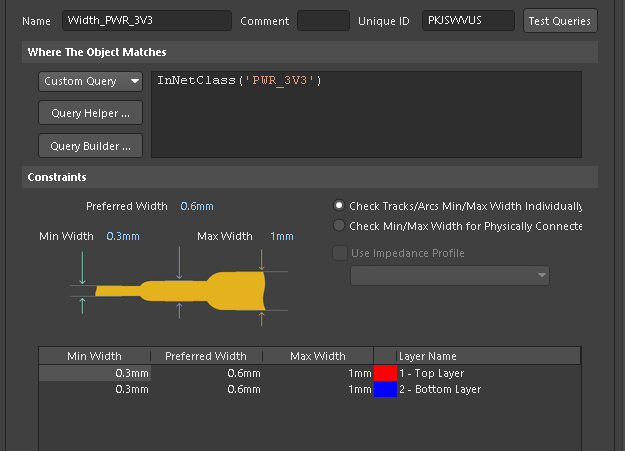
\includegraphics[width=1.05\textwidth]{Images/1.png}
%	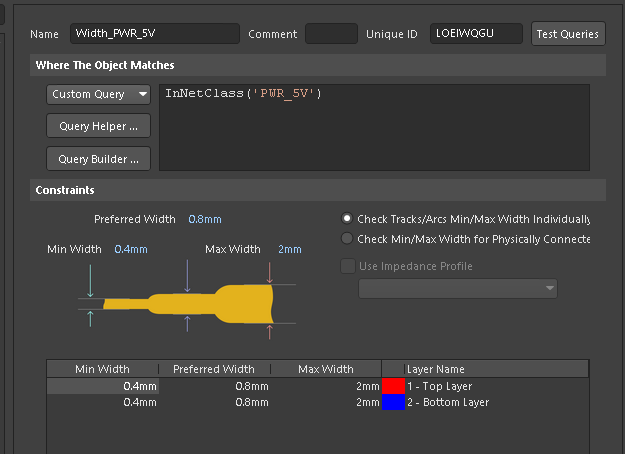
\includegraphics[width=0.75\textwidth]{Images/2.png}
%	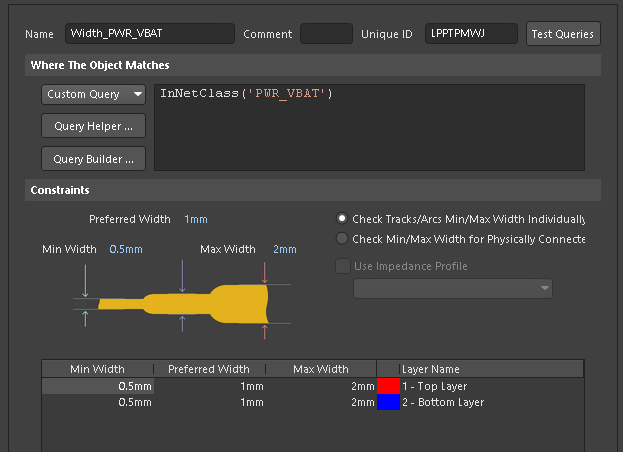
\includegraphics[width=0.75\textwidth]{Images/3.png}
	\vspace{2pt}\\
	{\footnotesize\textit{Nota.} Elaboración propia a partir del diseño en Altium Designer.}
\end{figure}

% =====================================================================
\subsection{Lista de materiales (BOM)}

La lista de materiales (\textit{Bill of Materials}, BOM) consolida todos los
componentes del dispositivo, organizados por bloque funcional: etapa de
alimentación de dos rieles basada en el convertidor reductor síncrono
TPS54302DDCR (12~V~$\rightarrow$~5~V) seguido de los reguladores lineales
AMS1117-3.3 y AP2112K-3.3TRG1 (5~V~$\rightarrow$~3,3~V), unidad de
procesamiento ESP32-S3-WROOM-1-N16R8 \citep{espressif_esp32_datasheet},
interfaz de bus CAN con el transceptor SN65HVD230
\citep{sn65hvd230_datasheet}, almacenamiento en MicroSD, interfaz de usuario
OLED y conector OBD-II. Los valores de los componentes pasivos de la etapa de
potencia se seleccionaron siguiendo el procedimiento de diseño y el
esquemático típico de aplicación del fabricante del regulador, detallado en
la subsección anterior. La Tabla~\ref{bom} presenta un resumen; el detalle de
fabricación (huellas, designadores agrupados y códigos de parte LCSC) se
presenta en el Apéndice~N.

% --------------------- Tabla BOM ---------------------
\begingroup
\captionsetup{labelformat=simple, labelsep=newline, textfont=it, labelfont=bf, justification=raggedright, singlelinecheck=false}
\small
\begin{longtable}{c p{5.9cm} p{3.0cm} c c}
	\caption{Lista de materiales (BOM) del dispositivo}
	\label{bom} \\
	\toprule
	\rowcolor[rgb]{0.851, 0.851, 0.851}
	\textbf{Ref.} & \textbf{Componente} & \textbf{Valor / Parte} & \textbf{Encap.} & \textbf{Cant.} \\
	\midrule
	\endfirsthead
	\multicolumn{5}{l}{\textit{Tabla~\ref{bom} (continuación)}} \\
	\toprule
	\rowcolor[rgb]{0.851, 0.851, 0.851}
	\textbf{Ref.} & \textbf{Componente} & \textbf{Valor / Parte} & \textbf{Encap.} & \textbf{Cant.} \\
	\midrule
	\endhead
	\midrule
	\multicolumn{5}{r}{\textit{Continúa en la siguiente página\ldots}} \\
	\endfoot
	\bottomrule
	\endlastfoot
		\multicolumn{5}{l}{\textit{Etapa de alimentación, riel 1 de 2 (12~V $\rightarrow$ 5~V, síncrona)}} \\
		U1 & Convertidor reductor (buck) síncrono & TPS54302DDCR & SOT-23-6 & 1 \\
		L1 & Inductor de potencia          & 10~\textmu H      & SMD    & 1 \\
		D2 & Diodo protección polaridad inv.& SS34 (3~A/40~V)  & SMA    & 1 \\
		F1 & Fusible reseteable PTC        & $I_{hold}\approx 1{,}5$~A & 1812 & 1 \\
		C1,C2 & Condensador de entrada     & 4,7~\textmu F / 50~V X7R & 1206 & 2 \\
		C3 & Condensador de entrada (HF)   & 0,01~\textmu F    & 0603 & 1 \\
		C4,C5 & Condensador de salida (44~\textmu F efectivos) & 22~\textmu F / 16~V X5R & 1206 & 2 \\
		C6 & Condensador de mejora transitoria & 75~pF         & 0603 & 1 \\
		R1 & Resistor divisor realim. (sup.) & 100~k$\Omega$   & 0603 & 1 \\
		R2 & Resistor divisor realim. (inf.) & 13,3~k$\Omega$  & 0603 & 1 \\
		\midrule
		\multicolumn{5}{l}{\textit{Etapa de alimentación, riel 2 de 2 (5~V $\rightarrow$ 3,3~V, dos rieles LDO)}} \\
		U4 & LDO riel 1 (ESP32-S3, hasta 1~A), siempre activo & AMS1117-3.3 & SOT-223 & 1 \\
		U5 & LDO riel 2 (periféricos, hasta 600~mA) & AP2112K-3.3TRG1 & SOT-23-5 & 1 \\
		C14,C15 & Desacople entrada/salida AMS1117 & 10~\textmu F & 1206 & 2 \\
		C16,C17 & Desacople entrada/salida AP2112 & 1~\textmu F & 0603 & 2 \\
		\midrule
		\multicolumn{5}{l}{\textit{Unidad de procesamiento}} \\
		U2 & Microcontrolador (módulo)     & ESP32-S3-WROOM-1-N16R8 & Módulo & 1 \\
		R3 & \textit{Pull-up} EN           & 10~k$\Omega$      & 0603 & 1 \\
		C7 & Condensador EN                & 0,1~\textmu F     & 0603 & 1 \\
		C8--C11 & Desacople de alimentación & 0,1~\textmu F    & 0603 & 4 \\
		C12 & Reserva de carga (\textit{bulk}) 3,3~V & 10~\textmu F & 0805 & 1 \\
		SW1 & Pulsador de \textit{reset}   & ---               & SMD  & 1 \\
		SW2 & Pulsador BOOT (GPIO0)        & ---               & SMD  & 1 \\
		\midrule
		\multicolumn{5}{l}{\textit{Interfaz de bus CAN}} \\
		U3 & Transceptor CAN               & SN65HVD230        & SOIC-8 & 1 \\
		R4 & Resistor de control de pendiente  & 10~k$\Omega$ & 0603 & 1 \\
		R5 & Resistor de terminación (opcional)$^{a}$ & 120~$\Omega$ & 0805 & 1 \\
		C13 & Desacople                    & 0,1~\textmu F     & 0603 & 1 \\
		\midrule
		\multicolumn{5}{l}{\textit{Almacenamiento y pantalla}} \\
		J2 & Zócalo MicroSD (push-push)    & ---               & SMD  & 1 \\
		R6--R9 & \textit{Pull-up} líneas SPI & 10~k$\Omega$    & 0603 & 4 \\
		DISP1 & Pantalla OLED I\textsuperscript{2}C 0,96" & SSD1306 & Módulo & 1 \\
		R10,R11 & \textit{Pull-up} I\textsuperscript{2}C (SDA/SCL) & 4,7~k$\Omega$ & 0603 & 2 \\
		\midrule
		\multicolumn{5}{l}{\textit{Conectores e indicadores}} \\
		J1 & Conector OBD-II (12~V, GND, CANH, CANL) & 4 pines & --- & 1 \\
		LED1 & LED indicador de alimentación & Verde           & 0805 & 1 \\
		LED2 & LED indicador de estado      & Azul             & 0805 & 1 \\
		R12,R13 & Resistor limitador de LED & 1~k$\Omega$       & 0805 & 2 \\
\end{longtable}
\endgroup

\vspace{2pt}
{\footnotesize\textit{Nota.} Elaboración propia. Los valores de la etapa de
	alimentación siguen el procedimiento de diseño del fabricante para el
	TPS54302DDCR, detallado en la subsección de diseño de hardware de este
	capítulo. $^{a}$El resistor de terminación de 120~$\Omega$ se
	deja como \textit{footprint} opcional (no poblado por defecto), dado que el
	dispositivo se conecta como nodo en derivación a un bus CAN que ya posee sus
	terminaciones en el vehículo.}

% =====================================================================
\subsection{Capacidades de fabricación de JLCPCB}

El PCB se fabricó mediante el servicio de prototipado de JLCPCB, integrado de
forma nativa con la herramienta EasyEDA empleada en el diseño. Para garantizar
una producción correcta y de alto rendimiento (\textit{Right-First-Time}), las
reglas de diseño (DRC) del proyecto se ajustaron a las capacidades del
fabricante para placas de dos capas en cobre de 1~oz \citep{JLCPCB2025}. La
Tabla~\ref{jlcpcb} compara los límites de fabricación con los valores adoptados
en este diseño, evidenciando que todos los parámetros se mantienen dentro de la
ventana de proceso estándar (la más económica y de mayor rendimiento de
producción).

% --------------------- Tabla capacidades JLCPCB ---------------------
\begin{table}[H]
	
	\captionsetup{labelformat=simple, labelsep=newline, textfont=it, labelfont=bf, justification=raggedright, singlelinecheck=false}
	\caption{Capacidades de fabricación de JLCPCB (2 capas, 1~oz) frente al diseño}
	\label{jlcpcb}
	\centering
	\begin{tabular}{p{5.2cm} c c}
		\toprule
		\rowcolor[rgb]{0.851, 0.851, 0.851}
		\textbf{Parámetro de fabricación} & \textbf{Mínimo JLCPCB} & \textbf{Diseño} \\
		\midrule
		Ancho mínimo de pista        & 0,127 mm (5 mil) & 0,20 mm \\
		Separación mínima de pista   & 0,127 mm (5 mil) & 0,20 mm \\
		Diámetro mínimo de perforación & 0,20 mm        & 0,30 mm \\
		Anillo anular mínimo         & 0,15 mm          & 0,15 mm \\
		Distancia cobre--borde       & 0,30 mm          & 0,30 mm \\
		Altura mínima de texto (serigrafía) & 1,00 mm   & $\geq 1$ mm \\
		Ancho mínimo de línea (serigrafía)  & 0,15 mm   & $\geq 0{,}15$ mm \\
		Expansión de máscara antisoldante   & 0,05 mm   & 0,05 mm \\
		Espesor de cobre             & 1 oz (35~\textmu m) & 1 oz \\
		Tamaño de placa (rango)      & 5$\times$5 a 400$\times$500 mm & 40$\times$60 mm \\
		\bottomrule
	\end{tabular}
	
	\vspace{2pt}
	{\footnotesize\textit{Nota.} Capacidades según la documentación de fabricación de
		JLCPCB \citep{JLCPCB2025}. Todos los valores del diseño cumplen o superan el
		mínimo del fabricante, situándose en la categoría de proceso estándar.}
\end{table}

% --------------------- FIGURA (marcador) --------------------
%Inserta aquí una captura del reporte DFM/DRC de JLCPCB o de la
% vista previa de Gerbers (cara superior/inferior) confirmando que el diseño
% pasa la verificación de fabricación. Reemplaza la ruta del \includegraphics.
\begin{figure}[H]
	\centering
	\caption{Verificación de fabricabilidad (DFM) del PCB en JLCPCB}
	\label{fig:jlcpcb_dfm}
	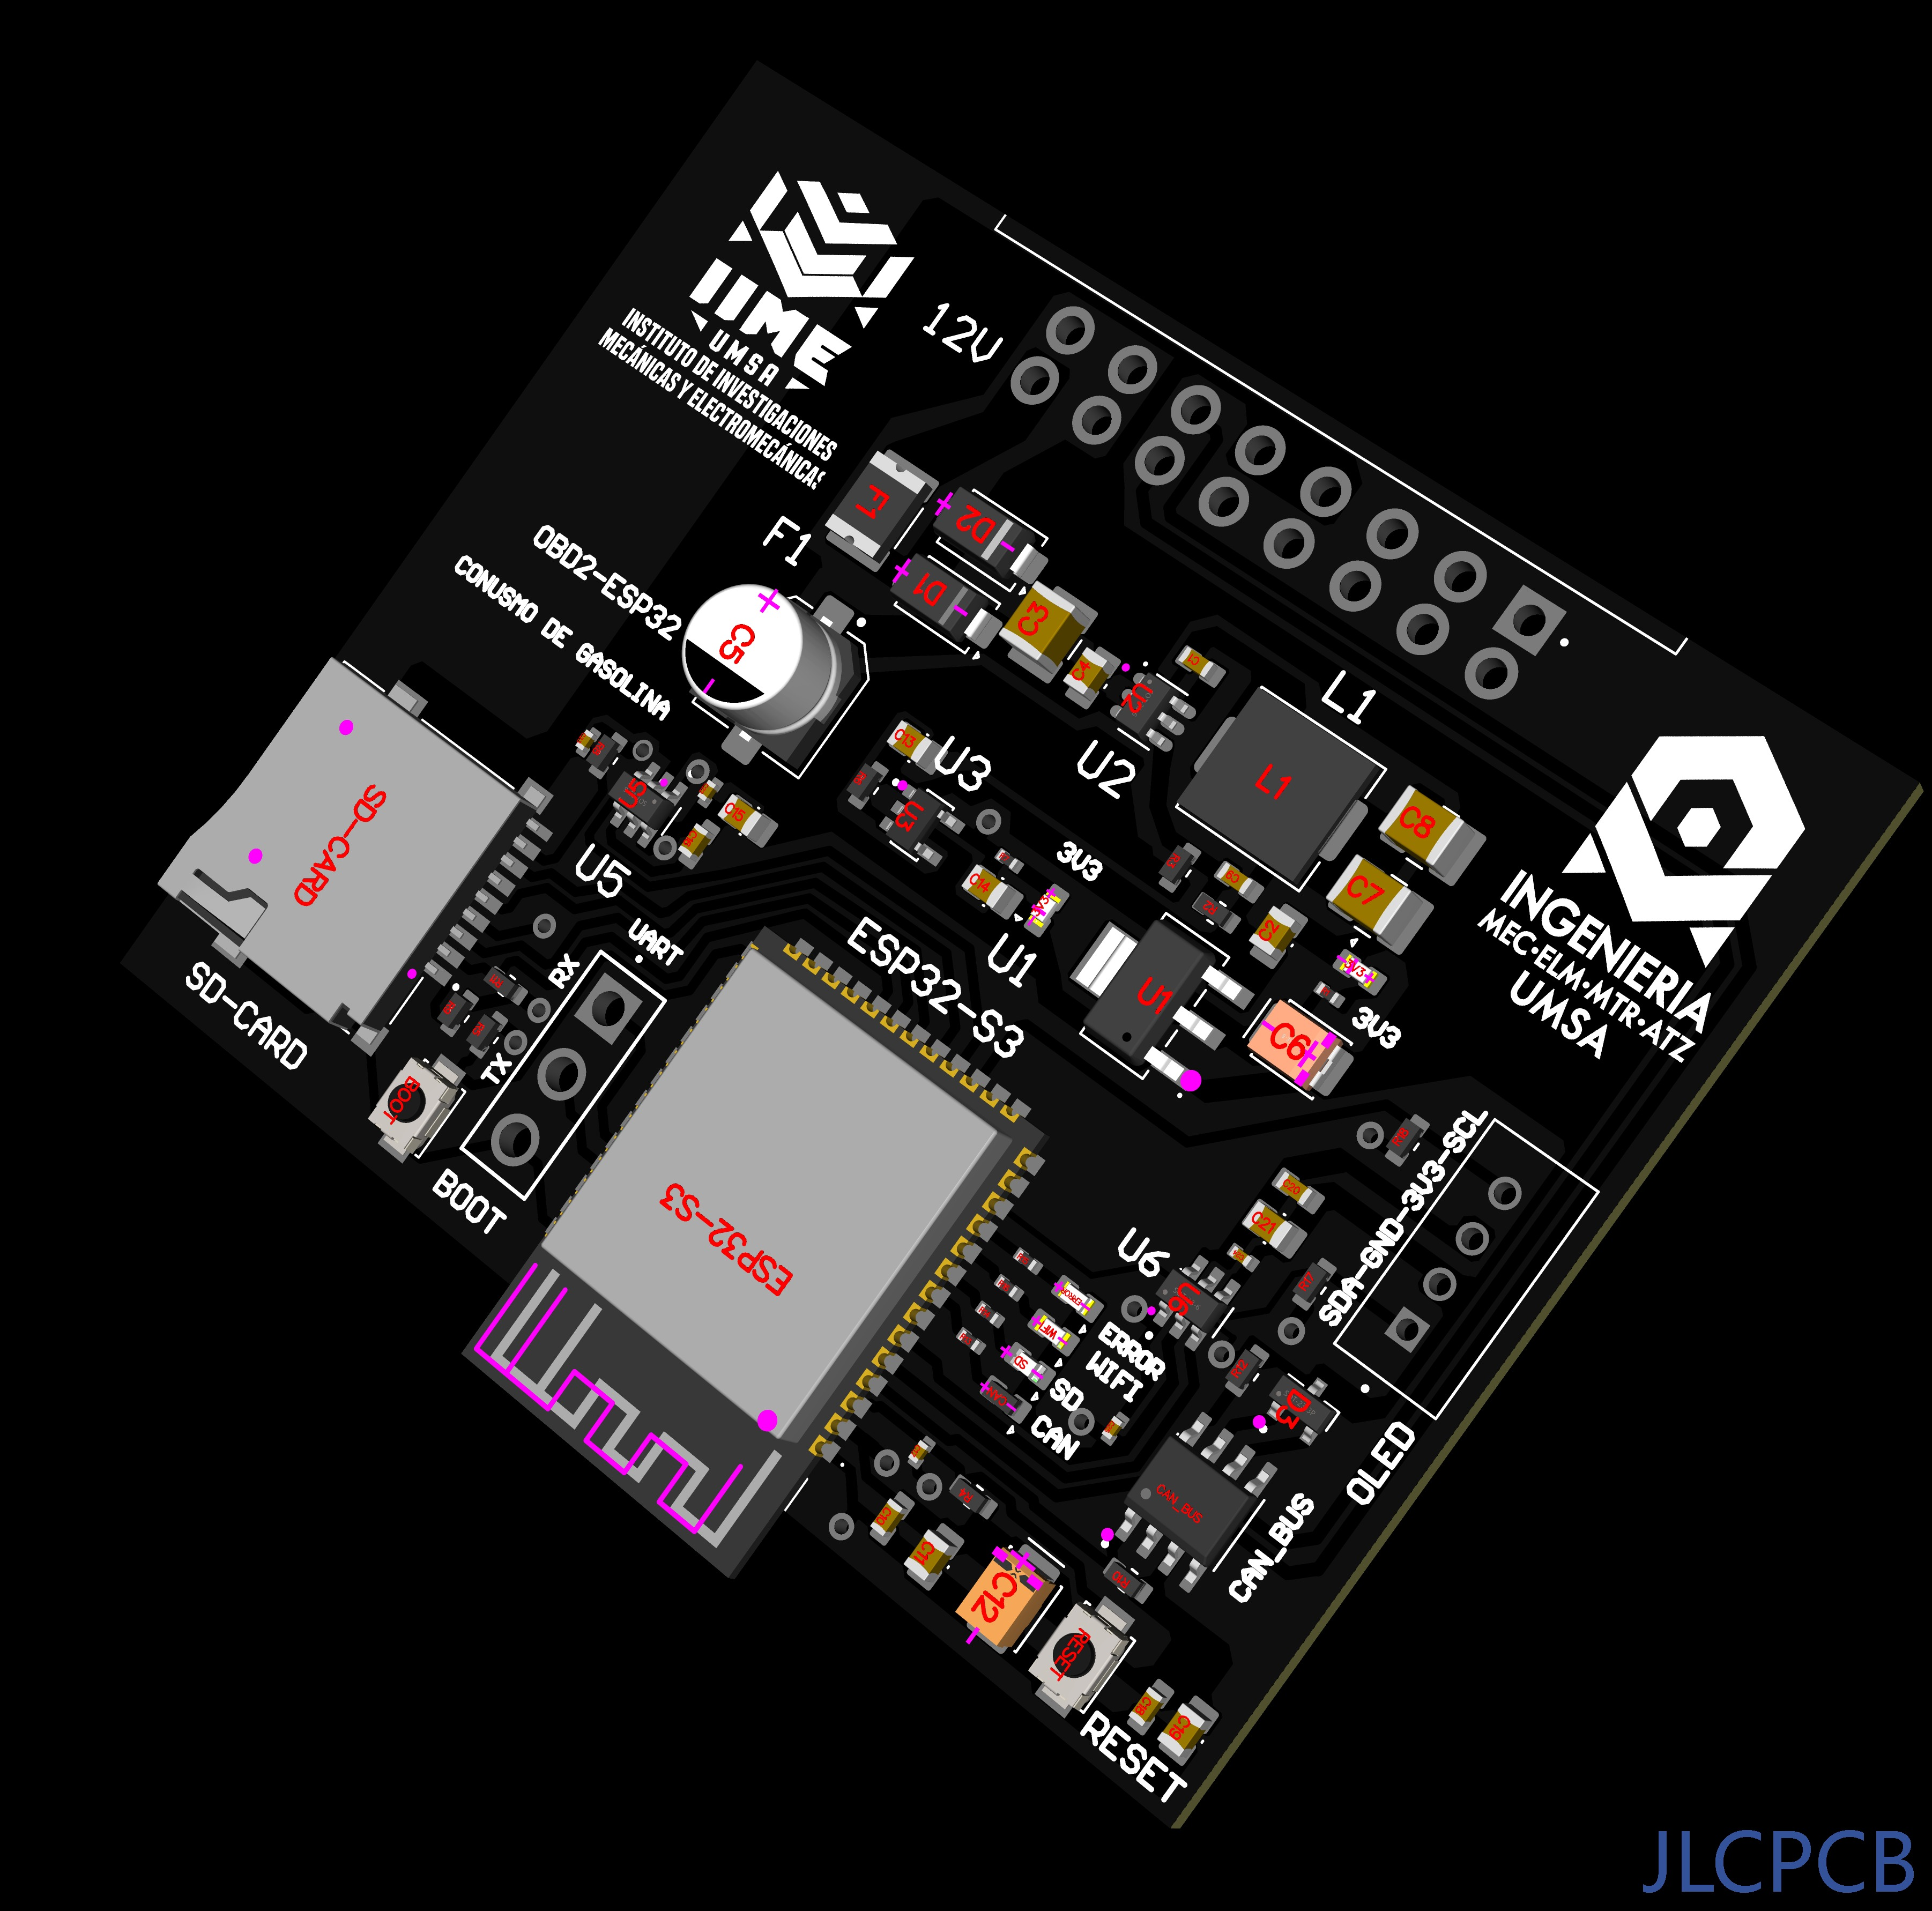
\includegraphics[width=0.8\textwidth]{Images/3D_PCB.png}
	
	\vspace{2pt}
	{\footnotesize\textit{Nota.} Captura obtenida del servicio de fabricación JLCPCB
		\citep{JLCPCB2025}.}
\end{figure}


\subsection{Diseño de la carcasa (impresión 3D)}

Aquí realizare el envase al PCB , cuando pida la PCB pondré aquí información.

% ────────────────────────────────────────────────────────────
% =====================================================================
%  SECCIÓN: MODELO MATEMÁTICO DE ESTIMACIÓN DE CONSUMO DE COMBUSTIBLE
%  Enfoque: deducción de ecuaciones desde principios físicos + criterios
%
%  PAQUETES REQUERIDOS (verificar en el preámbulo principal):
%     \usepackage{amsmath}
%     \usepackage{booktabs}
%     \usepackage{float}
%     \usepackage{graphicx}
%     \usepackage{array}
%     \usepackage[ruled,vlined,linesnumbered]{algorithm2e}  % pseudocódigo
%     \usepackage{tikz}                                      % diagrama de estados
%     \usetikzlibrary{shapes.geometric,arrows.meta,positioning}
%     \usepackage{natbib}                                    % citas APA 7
%
%  CONVENCIÓN APA 7: número/título de tabla y figura ARRIBA; "Nota." abajo.
% =====================================================================

\section{Modelo matemático de estimación de consumo de combustible}

En la sección 2.7 se desarrolló el marco teórico de los modelos de estimación de
consumo de combustible. En este apartado, en cambio, se deducen y formalizan las
ecuaciones que se implementarán directamente en el software del dispositivo,
partiendo de principios físicos (conservación de masa, ley de los gases ideales
y relación aire-combustible) y aplicando los criterios de ingeniería que rigen la
selección de variables, parámetros y fuentes de datos (PIDs OBD-II). El objetivo
es obtener un conjunto de expresiones cerradas, computables en tiempo real sobre
el ESP32, junto con conclusiones operativas sobre qué PIDs deben consultarse y
con qué prioridad.

% =====================================================================
\subsection{Método por sensor MAF}

El método más directo parte de la medición del flujo másico de aire admitido por
el motor, $\dot{m}_{air}$ [g/s], reportado por el sensor MAF (\textit{Mass Air
	Flow}) a través del PID 0x10 \citep{sae_j1979_2014}. La estimación de combustible
se fundamenta en la relación aire-combustible (\textit{Air-Fuel Ratio}, AFR),
definida como el cociente entre la masa de aire y la masa de combustible de la
mezcla \citep{Heywood2018}:

\begin{equation}
	\mathrm{AFR} = \frac{\dot{m}_{air}}{\dot{m}_{fuel}}
	\label{eq:afr}
\end{equation}

Para la gasolina, la relación estequiométrica es $\mathrm{AFR}_{s} \approx 14{,}7$
(14,7 kg de aire por cada kg de combustible) \citep{Heywood2018, Bosch2014}. La
mezcla real rara vez es exactamente estequiométrica; la ECU la regula en torno a
$\lambda = 1$, donde $\lambda$ es el factor lambda (relación de equivalencia
inversa) disponible en el PID 0x44. La relación real se expresa entonces como
$\mathrm{AFR} = \lambda \cdot \mathrm{AFR}_{s}$, y despejando $\dot{m}_{fuel}$ de
la Ecuación \ref{eq:afr} se obtiene el flujo másico de combustible:

\begin{equation}
	\dot{m}_{fuel} = \frac{\dot{m}_{air}}{\lambda \cdot \mathrm{AFR}_{s}}
	\label{eq:mfuel}
\end{equation}

El flujo másico se convierte a flujo volumétrico dividiendo por la densidad del
combustible, $\rho_{fuel} \approx 745$~kg/m$^3$ para la gasolina
\citep{Bosch2014}. Considerando que $1$~kg/m$^3 = 1$~g/L y que $\dot{m}_{air}$ se
expresa en g/s, el caudal de combustible en litros por hora (FuelRate) resulta de
incorporar el factor de conversión temporal $3600$~s/h:

\begin{equation}
	\mathrm{FuelRate}\;[\mathrm{L/h}]
	= \frac{3600 \cdot \dot{m}_{air}}{\lambda \cdot \mathrm{AFR}_{s} \cdot \rho_{fuel}}
	\label{eq:fuelrate_maf}
\end{equation}

Finalmente, el consumo normalizado por distancia, métrica de referencia para el
usuario, se obtiene relacionando el caudal con la velocidad del vehículo $v$
[km/h] (PID 0x0D):

\begin{equation}
	\mathrm{FC}\;[\mathrm{L/100\,km}]
	= \frac{\mathrm{FuelRate}\;[\mathrm{L/h}]}{v\;[\mathrm{km/h}]} \cdot 100
	\label{eq:fc}
\end{equation}

\noindent donde:

\begin{center}
	\begin{tabular}{r l}
		$\dot{m}_{air}$ & : flujo másico de aire [g/s] (PID 0x10) \\
		$\dot{m}_{fuel}$ & : flujo másico de combustible [g/s] \\
		$\mathrm{AFR}_{s}$ & : relación aire-combustible estequiométrica ($\approx 14{,}7$) \\
		$\lambda$ & : factor lambda (PID 0x44; $\lambda = 1$ en estequiometría) \\
		$\rho_{fuel}$ & : densidad de la gasolina ($\approx 745$~kg/m$^3$) \\
		$v$ & : velocidad del vehículo [km/h] (PID 0x0D) \\
	\end{tabular}
\end{center}

\textit{Criterio de ingeniería.} El método MAF es el más exacto porque mide
\emph{directamente} la masa de aire, sin requerir el modelado de la eficiencia
volumétrica ni el conocimiento de la cilindrada; su única dependencia paramétrica
es $\rho_{fuel}$ y el supuesto sobre $\lambda$. Su limitación es la
disponibilidad: exige que el vehículo soporte el PID 0x10, lo cual no está
garantizado (véase la Subsección \ref{subsec:soporte_pids}).

% =====================================================================
\subsection{Método Speed-Density}

Cuando el vehículo no dispone de sensor MAF (caso del Changan Honor analizado),
el flujo másico de aire no se mide sino que se \emph{estima} a partir de la
presión absoluta del múltiple (MAP, PID 0x0B), la temperatura del aire de
admisión (IAT, PID 0x0F) y el régimen del motor (RPM, PID 0x0C), junto con dos
parámetros del motor: la cilindrada $V_d$ y la eficiencia volumétrica $\eta_v$.
Este es el método \textit{Speed-Density} \citep{Heywood2018, Pulkrabek2014}.

El punto de partida es la ecuación de los gases ideales en su forma de densidad,
$P = \rho R T$, de la cual se despeja la densidad del aire de admisión
\citep{Cengel2019}:

\begin{equation}
	\rho_{air} = \frac{\mathrm{MAP}}{R_{air} \cdot \mathrm{IAT}}
	\label{eq:rho_air}
\end{equation}

\noindent con $R_{air} = 287$~J/(kg$\cdot$K) (constante específica del aire), MAP
en Pa e IAT en kelvin. A continuación se cuantifica el aire admitido por unidad
de tiempo. En un motor de cuatro tiempos, cada cilindro completa una carrera de
admisión una vez cada dos vueltas del cigüeñal; por lo tanto, el número de ciclos
de admisión completos por segundo es:

\begin{equation}
	n_{ciclos} = \frac{\mathrm{RPM}}{2} \cdot \frac{1}{60} = \frac{\mathrm{RPM}}{120}
	\label{eq:nciclos}
\end{equation}

El factor 120 surge del producto de dos conversiones: el factor 2 del ciclo de
cuatro tiempos (una admisión cada dos revoluciones) y el factor 60 del paso de
minutos a segundos. \textbf{Es crítico aplicar este factor una sola vez}: dividir
adicionalmente entre dos (un error frecuente, que confunde el ciclo de cuatro
tiempos con una segunda corrección) deja el resultado en la mitad de lo que debería ser.

En condiciones ideales, el volumen de aire admitido por ciclo es la cilindrada
$V_d$; la masa real admitida se corrige con la eficiencia volumétrica $\eta_v$.
Combinando la densidad (Ecuación \ref{eq:rho_air}) y la frecuencia de ciclos
(Ecuación \ref{eq:nciclos}), el flujo másico de aire estimado es:

\begin{equation}
	\dot{m}_{air} = \eta_v \cdot \rho_{air} \cdot V_d \cdot \frac{\mathrm{RPM}}{120}
	= \eta_v \cdot \frac{\mathrm{MAP}}{R_{air}\cdot \mathrm{IAT}} \cdot V_d \cdot \frac{\mathrm{RPM}}{120}
	\label{eq:speed_density}
\end{equation}

\noindent donde:

\begin{center}
	\begin{tabular}{r l}
		$\rho_{air}$ & : densidad del aire de admisión [kg/m$^3$] \\
		$\mathrm{MAP}$ & : presión absoluta del múltiple [Pa] (PID 0x0B) \\
		$R_{air}$ & : constante específica del aire ($287$~J/(kg$\cdot$K)) \\
		$\mathrm{IAT}$ & : temperatura del aire de admisión [K] (PID 0x0F) \\
		$V_d$ & : cilindrada total del motor [m$^3$] \\
		$\eta_v$ & : eficiencia volumétrica [adimensional] \\
		$\mathrm{RPM}$ & : régimen del motor [rev/min] (PID 0x0C) \\
	\end{tabular}
\end{center}

Una vez estimado $\dot{m}_{air}$ con la Ecuación \ref{eq:speed_density}, el flujo
de combustible y el consumo se calculan exactamente igual que en el método MAF,
mediante las Ecuaciones \ref{eq:mfuel} a \ref{eq:fc}. De este modo, ambos métodos
comparten la misma cadena de cálculo aguas abajo y solo difieren en cómo obtienen
$\dot{m}_{air}$.

\textit{Criterio de ingeniería.} El método Speed-Density habilita la estimación
en vehículos sin MAF, a costa de introducir dos dependencias paramétricas: $V_d$
(conocida y constante) y $\eta_v$ (variable con el punto de operación). Su
exactitud queda condicionada por la calidad del modelo de $\eta_v$ y por la
correcta lectura de la presión, factor especialmente sensible en altura, como se
analiza a continuación.

% =====================================================================
\subsection{Eficiencia volumétrica y corrección por altitud}
\label{subsec:etav-altitud}

La eficiencia volumétrica $\eta_v$ se define como el cociente entre la masa de
aire realmente admitida y la masa teórica que ocuparía la cilindrada a la densidad
del aire de admisión \citep{Heywood2018}:

\begin{equation}
	\eta_v = \frac{m_{air,\,real}}{\rho_{air}\cdot V_d}
	\label{eq:eta_v}
\end{equation}

En motores atmosféricos $\eta_v$ se sitúa típicamente entre 0,70 y 0,95, y varía
con el régimen y la carga \citep{Heywood2018, Pulkrabek2014}. En la implementación
se adopta un valor calibrado en función del punto de operación, ajustado de forma
adaptativa mediante la realimentación de los \textit{fuel trims} de la ECU (lazo
cerrado descrito en la arquitectura de control del sistema).

\subsubsection*{Efecto de la altitud de La Paz}

El parámetro físico determinante en altura es la presión atmosférica. La densidad
del aire (Ecuación \ref{eq:rho_air}) es directamente proporcional a la presión;
una sobreestimación de esta se traduce, punto por punto, en una sobreestimación
del aire admitido y, por tanto, del combustible calculado. La Paz se encuentra a
$\approx 3600$~m s.\,n.\,m., muy por encima de la referencia a nivel del mar
empleada por defecto en la mayoría de las implementaciones genéricas. La presión a
dicha altitud puede predecirse con el modelo de la Atmósfera Estándar
Internacional (ISA) \citep{ISO2533_1975}:

\begin{equation}
	P(h) = P_0 \left( 1 - \frac{L\,h}{T_0} \right)^{\dfrac{g\,M}{R\,L}}
	\label{eq:isa}
\end{equation}

\noindent con $P_0 = 101{,}32$~kPa, $T_0 = 288{,}15$~K, $L = 0{,}0065$~K/m,
$g = 9{,}80$~m/s$^2$, $M = 0{,}029$~kg/mol y $R = 8{,}32$~J/(mol$\cdot$K).
Evaluando la Ecuación \ref{eq:isa} en $h = 3600$~m se obtiene
$P(3600) \approx 64{,}9$~kPa, valor que coincide con la presión barométrica
medida en tiempo real mediante el PID 0x33 ($\approx 65$~kPa). Esta concordancia
valida tanto el modelo ISA como la lectura del sensor y confirma la magnitud de la
desviación respecto al nivel del mar.

El error cometido al asumir la presión estándar a nivel del mar
($P_0 = 101{,}3$~kPa) en lugar de la presión real de La Paz
($P_{baro} = 65$~kPa) es:

\begin{equation}
	\varepsilon = \frac{P_0 - P_{baro}}{P_{baro}}
	= \frac{101{,}3 - 65}{65} \approx 0{,}558 = 55{,}8\%
	\label{eq:error_altitud}
\end{equation}

Es decir, un modelo que \emph{asumiera} una presión de admisión constante de
nivel del mar en vez de medirla sobrestimaría el consumo en aproximadamente un
\textbf{55,8\%} en La Paz, una desviación inadmisible para la finalidad del
dispositivo.

\textit{Precisión importante.} La Ecuación~\eqref{eq:speed_density} de este
proyecto \emph{no} incurre en este error, porque no asume $P_0$: emplea en
cada ciclo la lectura real y absoluta del colector ($\mathrm{MAP}$, PID
0x0B) tomada directamente de la ECU del vehículo. A mariposa cerrada, el
MAP no puede superar la presión atmosférica local, sea cual sea esta; por
construcción, la densidad del aire calculada con la Ecuación~\ref{eq:rho_air}
ya refleja la altitud de operación sin necesitar ningún factor adicional.
Aplicar además un multiplicador $K_{alt} = P_{baro}/P_0$ sobre el resultado
(como haría una implementación que combinara MAP real \emph{y} un factor de
altitud) penalizaría la altitud dos veces sobre el mismo dato, y así se
incurriría en un error de signo contrario. Por esta razón, el firmware evaluado en el
Capítulo~4 no aplica $K_{alt}$ como corrector multiplicativo.

El valor de $P_{baro}$ conserva, no obstante, una utilidad real: como
\textbf{dato de validación} del propio sensor MAP, no como corrector del
cálculo. Con el contacto puesto y el motor apagado (\textit{key-on,
engine-off}), no existe vacío de admisión, por lo que el MAP debería leer
un valor muy cercano a la presión atmosférica real; contrastar esa lectura
contra el PID 0x33 (o, en su defecto, contra el modelo ISA evaluado en la
altitud del sitio) permite verificar que el sensor MAP del vehículo está
correctamente calibrado para la altitud de La Paz, antes de confiar en él
durante la conducción. Esta es la prueba que se documenta en el
Capítulo~4.

\textit{Criterio de ingeniería.} Se prioriza la medición en tiempo real del PID
0x33 sobre el modelo ISA estático como fuente de $P_{baro}$ para esta
validación, ya que la primera captura también las variaciones meteorológicas
de presión; el modelo ISA se reserva como respaldo (\textit{fallback}) cuando
el vehículo no soporta el PID 0x33 (implementado así en
\texttt{can\_obd2.cpp}, función \texttt{isaPressureKpaAt()}). La corrección
de altitud del \emph{consumo} es, en cambio, automática e implícita en el
método Speed-Density con MAP real, y no requiere un paso adicional de
software.

% =====================================================================
\subsection{Comparativa de métodos y criterio de selección}

La Tabla~\ref{tab:estim} sintetiza las diferencias entre ambos métodos. El
criterio de selección es jerárquico y se fundamenta en un principio de ingeniería:
preferir siempre la medición directa frente a la estimación basada en
	modelos. En consecuencia, si el vehículo soporta el sensor MAF (PID 0x10) se
emplea el método MAF; en caso contrario, se recurre al método Speed-Density. La
Tabla~\ref{tab:criterio_seleccion} resume este árbol de decisión, y la
Subsección \ref{subsec:soporte_pids} detalla cómo se determina el soporte de
PIDs en tiempo de ejecución.

% --------------------- Tabla: criterio de selección ---------------------
\begin{table}[H]
	
	\captionsetup{labelformat=simple, labelsep=newline, textfont=it, labelfont=bf, justification=raggedright, singlelinecheck=false}
	\caption{Árbol de decisión para la selección del método de estimación}
	\centering
	\label{tab:criterio_seleccion}
	\begin{tabular}{p{5.0cm} c p{5.0cm}}
		\toprule
		\rowcolor[rgb]{0.851, 0.851, 0.851}
		\textbf{Condición evaluada} & \textbf{Resultado} & \textbf{Método seleccionado} \\
		\midrule
		PID 0x10 (MAF) soportado & Verdadero & Método MAF (medición directa) \\[3pt]
		PID 0x10 (MAF) soportado & Falso & Método Speed-Density (estimación) \\[3pt]
		PID 0x0B, 0x0C, 0x0F soportados & Requerido & Habilita Speed-Density como respaldo \\
		\bottomrule
	\end{tabular}
	
	\vspace{2pt}
	{\footnotesize\textit{Nota.} Elaboración propia. La evaluación se realiza una sola
		vez durante la inicialización, a partir de la respuesta al PID 0x00
		\citep{sae_j1979_2014}.}
\end{table}

El pseudocódigo del criterio de conmutación, en su forma más simple, es:

\begin{algorithm}[H]
	\DontPrintSemicolon
	\SetKwInOut{Entrada}{Entrada}\SetKwInOut{Salida}{Salida}
	\Entrada{Mapa de PIDs soportados (respuesta a PID 0x00)}
	\Salida{Método de estimación seleccionado}
	\BlankLine
	\eIf{PID\_0x10\_soportado}{
		metodo $\leftarrow$ \textsc{MAF}\;
	}{
		metodo $\leftarrow$ \textsc{Speed-Density}\;
	}
	\Return metodo\;
	\caption{Criterio de selección del método de estimación}
	\label{alg:seleccion}
\end{algorithm}

% =====================================================================
\subsection{Consulta de soporte de PIDs (PID 0x00)}
\label{subsec:soporte_pids}

La decisión anterior exige conocer, en tiempo de ejecución, qué PIDs implementa
cada vehículo. El estándar SAE J1979 resuelve esto mediante el PID 0x00, cuya
respuesta es un campo de bits (\textit{bitmask}) de cuatro bytes (denominados A,
B, C y D) que codifica el soporte de los PIDs 0x01 a 0x20
\citep{sae_j1979_2014}. La convención de codificación es la siguiente: el byte A es
el más significativo, y dentro de cada byte el bit 7 es el más significativo y el
bit 0 el menos significativo. El bit más significativo del byte A corresponde al
PID 0x01, y así sucesivamente hasta el bit menos significativo del byte D, que
corresponde al PID 0x20. Un bit en 1 indica que el PID asociado está soportado.

De esta convención se desprende un resultado de gran utilidad para este proyecto:
el soporte del sensor MAF (PID 0x10) queda determinado por el bit menos
	significativo del byte B. La Tabla~\ref{tab:bitmap} muestra el mapeo de los bits
del byte B (que abarca los PIDs 0x09 a 0x10, precisamente los más relevantes para
la estimación de consumo) y un ejemplo de decodificación.

% --------------------- Tabla: decodificación bitmask byte B ---------------------
\begin{table}[H]
	\captionsetup{labelformat=simple, labelsep=newline, textfont=it, labelfont=bf, justification=raggedright, singlelinecheck=false}	
	\caption{Decodificación del byte B de la respuesta al PID 0x00 (ejemplo: B = 0x3E)}
	\centering
	\label{tab:bitmap}
	\begin{tabular}{c c l c}
		\toprule
		\rowcolor[rgb]{0.851, 0.851, 0.851}
		\textbf{Bit (byte B)} & \textbf{PID} & \textbf{Parámetro} & \textbf{Ejemplo (0x3E)} \\
		\midrule
		7 & 0x09 & Presión de combustible            & 0 (no) \\
		6 & 0x0A & Presión de combustible (ECU)      & 0 (no) \\
		5 & 0x0B & MAP --- presión del múltiple      & 1 (sí) \\
		4 & 0x0C & RPM --- régimen del motor         & 1 (sí) \\
		3 & 0x0D & Velocidad del vehículo            & 1 (sí) \\
		2 & 0x0E & Avance de encendido               & 1 (sí) \\
		1 & 0x0F & IAT --- temperatura de admisión   & 1 (sí) \\
		0 & 0x10 & \textbf{MAF --- flujo másico de aire} & \textbf{0 (no)} \\
		\bottomrule
	\end{tabular}
	
	\vspace{2pt}
	{\footnotesize\textit{Nota.} Codificación según SAE J1979 \citep{sae_j1979_2014}.
		En el ejemplo, $\mathrm{0x3E} = 0011\,1110_2$: el bit 0 (MAF) está en 0, por lo que
		el vehículo \emph{no} soporta el PID 0x10 y el sistema conmuta a Speed-Density;
		los PIDs MAP, RPM, velocidad e IAT (bits 5 a 1) sí están disponibles, habilitando
		dicho método. Este patrón ilustra el caso de un vehículo sin sensor MAF.}
\end{table}

Cabe señalar que el PID 0x33 (presión barométrica), necesario para la corrección
por altitud, pertenece al rango 0x21--0x40; su soporte se consulta con el PID 0x20
de forma análoga. A partir de esta lectura de soporte, el dispositivo determina si
dispone de los PIDs que requiere cada método de estimación. La
Tabla~\ref{tab:pids_metodo} reúne los PIDs necesarios para el método MAF y para el
método Speed-Density, indicando en cada caso si la lectura es obligatoria u
opcional.

% --------------------- Tabla: PIDs requeridos por método ---------------------
\begin{table}[H]
	\captionsetup{labelformat=simple, labelsep=newline, textfont=it, labelfont=bf, justification=raggedright, singlelinecheck=false}
	\caption{PIDs requeridos por cada método de estimación}
	\centering
	\label{tab:pids_metodo}
	\begin{tabular}{c l c c}
		\toprule
		\rowcolor[rgb]{0.851, 0.851, 0.851}
		\textbf{PID} & \textbf{Parámetro} & \textbf{Método MAF} & \textbf{Speed-Density} \\
		\midrule
		0x00 & Descubrimiento de PIDs soportados      & Obligatorio & Obligatorio \\
		0x0C & RPM --- régimen del motor              & ---         & Obligatorio \\
		0x0B & MAP --- presión del múltiple           & ---         & Obligatorio \\
		0x0F & IAT --- temperatura de admisión        & ---         & Obligatorio \\
		0x10 & MAF --- flujo másico de aire           & Obligatorio & ---         \\
		0x0D & Velocidad del vehículo                 & Obligatorio & Obligatorio \\
		0x33 & Presión barométrica (altitud)          & ---         & Obligatorio$^{a}$ \\
		0x44 & Lambda --- relación de equivalencia    & Opcional    & Opcional \\
		\bottomrule
	\end{tabular}
	
	\vspace{2pt}
	{\footnotesize\textit{Nota.} Elaboración propia con base en SAE J1979
		\citep{sae_j1979_2014}.}
\end{table}

\textit{Conclusión sobre los PIDs.} El conjunto mínimo de PIDs que el dispositivo
debe consultar de forma obligatoria es: 0x00 (descubrimiento de soporte), 0x0C
(RPM), 0x0D (velocidad), y según el método, 0x10 (MAF) o bien
\{0x0B, 0x0F\} (MAP e IAT) más 0x33 (corrección por altitud). El PID 0x44
(lambda) se consulta para refinar la mezcla cuando está disponible; si no lo está,
se asume $\lambda = 1$.

% =====================================================================
\subsection{Algoritmo de conmutación automática}

La lógica completa de operación se modela como una máquina de estados finitos que
integra el descubrimiento de PIDs, la selección de método y el bucle de
adquisición. El sistema transita por cuatro estados, ilustrados en la
Figura~\ref{fig:fsm}: inicialización (INIT), verificación de MAF (CHECK\_MAF),
y los dos modos de operación (MAF\_MODE o SD\_MODE), que convergen al estado de
ejecución continua (RUNNING).

% --------------------- FIGURA: máquina de estados (TikZ) ---------------------
\begin{figure}[H]
	\centering
	\caption{Máquina de estados del algoritmo de conmutación automática}
	\label{fig:fsm}
	\vspace{4pt}
	\begin{tikzpicture}[
		node distance=14mm and 16mm,
		estado/.style={rectangle, rounded corners, draw, thick, minimum width=22mm, minimum height=9mm, align=center, font=\small},
		modo/.style={rectangle, rounded corners, draw, thick, fill=black!5, minimum width=24mm, minimum height=9mm, align=center, font=\small},
		flecha/.style={-{Stealth[length=2.4mm]}, thick},
		etiqueta/.style={font=\scriptsize, align=center}
		]
		\node[estado] (init) {INIT};
		\node[estado, right=of init] (check) {CHECK\_MAF};
		\node[modo, above right=8mm and 18mm of check] (maf) {MAF\_MODE};
		\node[modo, below right=8mm and 18mm of check] (sd) {SD\_MODE};
		\node[estado, below right=8mm and 18mm of maf] (run) {RUNNING};
		
		\draw[flecha] (init) -- node[etiqueta, above]{consulta\\PID 0x00} (check);
		\draw[flecha] (check) -- node[etiqueta, above left]{PID 0x10 = 1} (maf);
		\draw[flecha] (check) -- node[etiqueta, below left]{PID 0x10 = 0} (sd);
		\draw[flecha] (maf) -- node[etiqueta, above right]{$\dot{m}_{air}$ directo} (run);
		\draw[flecha] (sd) -- node[etiqueta, below right]{Speed-Density\\+ PID 0x33} (run);
		\draw[flecha]
		(run.south)
		|- ++(0,-20mm)
		-| node[pos=0.25, below]{bucle de adquisición}
		(init.south);
	\end{tikzpicture}
	
	\vspace{2pt}
	{\footnotesize\textit{Nota.} Elaboración propia. La transición desde CHECK\_MAF se
		decide con el bit 0 del byte B de la respuesta al PID 0x00.}
\end{figure}

El Algoritmo~\ref{alg:conmutacion} formaliza el comportamiento de la máquina de
estados, incluyendo la corrección por altitud en el modo Speed-Density.

\begin{algorithm}[H]
	\DontPrintSemicolon
	\SetKwInOut{Entrada}{Entrada}\SetKwInOut{Salida}{Salida}
	\Entrada{Tramas OBD-II del bus CAN; parámetros del motor $V_d$, $\eta_v$}
	\Salida{FuelRate [L/h], FC [L/100 km]}
	\BlankLine
	\textbf{Estado} INIT\;
	\quad Inicializar bus CAN (TWAI, 500 kbps); solicitar PID 0x00 y 0x20\;
	\quad soporte $\leftarrow$ decodificar\_bitmask(respuesta)\;
	\BlankLine
	\textbf{Estado} CHECK\_MAF\;
	\eIf{soporte[0x10]}{
		modo $\leftarrow$ \textsc{MAF\_MODE}\;
	}{
		modo $\leftarrow$ \textsc{SD\_MODE}\;
	}
	\BlankLine
	\textbf{Estado} RUNNING \textbf{(bucle periódico)}\;
	\While{sistema activo}{
		\eIf{modo = \textsc{MAF\_MODE}}{
			$\dot{m}_{air} \leftarrow$ leer\_PID(0x10)\;
		}{
			MAP $\leftarrow$ leer\_PID(0x0B);\quad IAT $\leftarrow$ leer\_PID(0x0F)\;
			RPM $\leftarrow$ leer\_PID(0x0C)\;
			\If{soporte[0x33]}{
				$P_{baro} \leftarrow$ leer\_PID(0x33)\tcp*{corrección por altitud}
			}
			$\rho_{air} \leftarrow \mathrm{MAP}/(R_{air}\cdot \mathrm{IAT})$\;
			$\dot{m}_{air} \leftarrow \eta_v \cdot \rho_{air} \cdot V_d \cdot \mathrm{RPM}/120$\;
		}
		$\lambda \leftarrow$ leer\_PID(0x44) \textbf{si} disponible \textbf{si no} $1$\;
		$\dot{m}_{fuel} \leftarrow \dot{m}_{air} / (\lambda \cdot 14{,}7)$\;
		FuelRate $\leftarrow 3600 \cdot \dot{m}_{fuel} / \rho_{fuel}$\;
		$v \leftarrow$ leer\_PID(0x0D)\;
		\If{$v > 0$}{
			FC $\leftarrow 100 \cdot$ FuelRate $/\, v$\;
		}
		Mostrar/registrar (FuelRate, FC); acumular litros y costo\;
	}
	\caption{Conmutación automática y cálculo de consumo}
	\label{alg:conmutacion}
\end{algorithm}

\textit{Criterio de ingeniería.} El descubrimiento de PIDs y la selección de
método se ejecutan una sola vez en la inicialización (no en cada iteración),
minimizando el tráfico en el bus CAN y la carga de cómputo del ESP32. El bucle
RUNNING opera a una frecuencia de muestreo acorde con la dinámica del consumo
(del orden de 1--5 Hz), suficiente para integrar litros y costo con exactitud sin
saturar el canal de diagnóstico.

\textit{Alcance de la implementación evaluada.} El Algoritmo~\ref{alg:conmutacion}
formaliza el \emph{criterio de diseño} que justifica la elección del método de
estimación: dado que el vehículo de prueba principal (Changan Honor) no soporta
el PID 0x10 (Subsección~\ref{subsec:soporte_pids}), Speed-Density es la única vía
disponible sin instalar un sensor adicional, y ese es el método que el firmware
descrito en la Sección~\ref{sec:software} fija de forma permanente para ambos
vehículos de validación del Capítulo~4 (incluido el Nissan Vanette, que sí soporta
el PID 0x10, pero se evalúa igualmente en modo Speed-Density para mantener un
único método comparable entre ambas unidades). La conmutación
\emph{automática y en tiempo de ejecución} entre MAF\_MODE y SD\_MODE que
describe el estado CHECK\_MAF de la máquina de estados no está implementada en
esta versión del firmware; se documenta aquí como la extensión natural del
sistema y se retoma como recomendación de trabajo futuro en el
Capítulo~6.
% ────────────────────────────────────────────────────────────
% ==============================================================================
%  SECCIÓN: Sistema de estimación con retroalimentación en lazo cerrado
%  Tesis: Sistema de monitoreo de consumo de combustible OBD-II (ESP32 + SN65HVD230)
%  Autor: Erick — Ing. Mecatrónica, UMSA (La Paz, Bolivia)
% ------------------------------------------------------------------------------
%  PAQUETES REQUERIDOS (agregar al preámbulo si aún no los tienes):
%    \usepackage{amsmath, amssymb}
%    \usepackage{booktabs}
%    \usepackage{array}
%    \usepackage{graphicx}
%    \usepackage{tikz}
%      \usetikzlibrary{arrows.meta, positioning, calc, shapes.geometric}
%    \usepackage{pgfplots}
%      \pgfplotsset{compat=1.18}
%    \usepackage[ruled,vlined,linesnumbered]{algorithm2e}
%    \usepackage[round]{natbib}   % estilo apalike / APA
%  COMPILADOR: PDFLaTeX (coherente con tu uso de \includepdf en apéndices)
% ==============================================================================

\section{Sistema de estimación con retroalimentación en lazo cerrado}
\label{sec:lazo-cerrado}

\textit{Alcance de esta sección: estudio y diseño, no implementación.} Todo lo
desarrollado a continuación —el factor de calibración adaptativo $K$ con
filtro EMA (Subsección~\ref{subsec:factor-k}), la identificación en línea de
la curva $\eta_v(N)$ por regresión (Subsección~\ref{subsec:curva-etav}) y la
conmutación automática MAF/Speed-Density (Subsección~\ref{subsec:soporte_pids})—
es un estudio y diseño formal de una arquitectura de estimador en
lazo cerrado, no una implementación evaluada en este proyecto. Del
contenido de esta sección, el firmware probado en el Capítulo~4 incorpora
únicamente el corrector directo por ajustes de combustible del ECU
($\mathrm{STFT}+\mathrm{LTFT}$ aplicados sobre el AFR efectivo, ya descrito en
la Sección~\ref{sec:speeddensity} del \emph{Diseño de software}); el resto
queda formalizado matemáticamente, pero sin construirse ni probarse en campo.

No se implementó por dos razones concretas, no por falta de desarrollo
matemático: primero, cada uno de los tres componentes exige su propio
protocolo de validación experimental independiente —un banco de pruebas con
carga controlada para calibrar y verificar el factor $K$, y sesiones de
conducción dedicadas para identificar $\eta_v(N)$ en línea sin reutilizar los
datos ya empleados en la calibración estática del Capítulo~4—, lo que excede
el tiempo disponible de un proyecto de grado si se suma al protocolo de
validación en lazo abierto ya reportado en ese capítulo. Segundo, se priorizó
deliberadamente contar con un sistema simple e íntegramente verificable,
coherente con lo efectivamente probado en campo, en vez de uno más
sofisticado pero sin evidencia experimental propia que respalde reportarlo
como validado; el Capítulo~6 retoma los tres componentes como trabajo futuro
concreto. Esta distinción entre lo formalizado y lo implementado se mantiene
explícita a lo largo de toda la sección, para que el lector no infiera
validación experimental de componentes que aún no se han puesto a prueba.

El método Speed-Density desarrollado en la sección anterior entrega una estimación
\emph{en lazo abierto} del flujo de aire y, por consiguiente, del consumo de
combustible. Esta sección formaliza por qué dicha estimación es insuficiente por sí
sola y cómo se la corrige incorporando la realimentación que el propio ECU del
vehículo expone a través del puerto OBD-II. El resultado es un \textbf{estimador en
	lazo cerrado} cuyo modelo matemático final, con todas sus variables de entrada y de
salida, se consolida al cierre de la sección.

% ------------------------------------------------------------------------------
\subsection{Justificación del enfoque en lazo cerrado}
\label{subsec:justificacion-lazo}

\subsubsection*{Limitaciones de la estimación en lazo abierto}

La estimación Speed-Density reposa sobre la ecuación de llenado del motor, en la que
la eficiencia volumétrica $\eta_v$ y los sensores de presión ($P_{\text{MAP}}$) y
temperatura ($T_{\text{IAT}}$) determinan por completo el flujo de aire estimado.
En un sistema embebido de bajo costo, sin acceso a banco dinamométrico, las
principales fuentes de error son:

\begin{itemize}
	\item \textbf{Incertidumbre de $\eta_v$.} La eficiencia volumétrica no es un dato
	de fábrica y varía con el régimen del motor, el envejecimiento mecánico y la
	apertura de válvulas. Un error del $10\,\%$ en $\eta_v$ se traslada
	directamente como un error del $10\,\%$ en el caudal de combustible
	\citep{Heywood2018}.
	\item \textbf{Ruido y cuantización de sensores.} Las PID OBD-II entregan
	$P_{\text{MAP}}$ con resolución de $1\,\mathrm{kPa}$ y $T_{\text{IAT}}$ con
	resolución de $1\,^{\circ}\mathrm{C}$; ambos propagan ruido a la densidad
	$\rho$ del modelo.
	\item \textbf{Condición no estequiométrica.} En enriquecimiento (aceleración a
	plena carga, arranque en frío) la relación aire--combustible se aparta de la
	estequiométrica, por lo que asumir $\lambda=1$ introduce un sesgo sistemático.
	\item \textbf{Deriva de $\eta_v$ con el envejecimiento.} A diferencia del efecto
	de altitud (ya resuelto por construcción al usar el MAP real en cada ciclo,
	como se explicó en la Subsección~\ref{subsec:etav-altitud}), la eficiencia
	volumétrica sí puede derivar con el tiempo (desgaste de válvulas, depósitos de
	carbón, calidad variable del combustible), y esa deriva no la corrige ningún
	sensor que el vehículo ya reporte por sí solo.
\end{itemize}

Al integrarse en el tiempo para obtener el consumo acumulado ($\mathrm{L}$ totales),
estos errores no se cancelan, sino que se acumulan como deriva. Se requiere, por
tanto, una señal de referencia que corrija la estimación de forma continua.

\subsubsection*{El ECU como lazo cerrado físico}

El ECU del vehículo opera un lazo de control de combustible cerrado: mediante la
sonda de oxígeno (lambda) mide la relación aire--combustible real y ajusta el tiempo
de inyección para sostener la relación objetivo. Este ajuste se publica en el bus
como ajustes de combustible(fuel trims): el ajuste de corto plazo
$\mathrm{STFT}$ (PID~\texttt{0x06}) y el de largo plazo $\mathrm{LTFT}$
(PID~\texttt{0x07}). En consecuencia, el lazo cerrado físico ya existe en el
	vehículo; nuestra contribución es observarlo y emplear su señal de corrección
para realimentar la estimación propia \citep{guzzella2010}.

\subsubsection*{Estimador, no controlador: el marco del observador}

Es necesaria una precisión conceptual que sostiene la defensa de este trabajo. El
módulo desarrollado no actúa sobre los inyectores; es un dispositivo de
monitoreo. Por ello no constituye un controlador en el sentido clásico, sino
un estimador en lazo cerrado (sensor virtual). Su arquitectura reproduce la
estructura predicción--corrección de un observador de estados
\citep{astrom2008}:

\begin{itemize}
	\item \emph{Predicción}: el modelo Speed-Density estima en lazo abierto el flujo
	de aire y de combustible a partir de $N$, $P_{\text{MAP}}$ e $T_{\text{IAT}}$.
	\item \emph{Corrección (innovación)}: los fuel trims del ECU, que codifican la
	medición real de la sonda lambda, corrigen la predicción.
\end{itemize}

De este modo, la planta es el motor; el controlador físico es el lazo de lambda del
ECU; y el algoritmo aquí propuesto es el observador que se realimenta de la señal de
corrección de ese controlador. Esta interpretación es directamente análoga al paso de
actualización de un observador de Luenberger o de un filtro de Kalman, y responde de
forma rigurosa a la pregunta de dónde reside el lazo cerrado del sistema.

% ------------------------------------------------------------------------------
\subsection{Arquitectura del lazo cerrado}
\label{subsec:arquitectura}

La Figura~\ref{fig:diagrama-lazo} presenta el diagrama de bloques del estimador. Se
distinguen cinco bloques funcionales: (1)~adquisición de señales OBD-II;
(2)~modelo base Speed-Density (predicción en lazo abierto); (3)~corrector
multiplicativo, que aplica la realimentación rápida del ECU; (4)~bloque de
aprendizaje adaptativo, que ajusta lentamente el factor de calibración $K$ (y,
opcionalmente, la curva $\eta_v$); y (5)~cálculo de métricas de salida.

\begin{figure}[H]
	% Formato APA 7 
	\captionsetup{labelformat=simple, labelsep=newline, textfont=it, labelfont=bf, justification=raggedright, singlelinecheck=false}
	\caption[Diagrama de bloques del estimador de consumo]{Diagrama de bloques del estimador de consumo en lazo cerrado.}
	\label{fig:diagrama-lazo}
	\centering
	
	\vspace{4mm}
	\begin{tikzpicture}[
		font=\small,
		block/.style={rectangle, draw, rounded corners, align=center,
			minimum height=1.05cm, minimum width=2.5cm, thick},
		io/.style={trapezium, trapezium left angle=70, trapezium right angle=110,
			draw, align=center, minimum height=1.0cm, thick},
		sum/.style={circle, draw, minimum size=0.55cm, thick, inner sep=0pt},
		line/.style={-{Latex[length=2mm]}, thick}
		]
		% 1. Fila principal
		\node[io] (sensores) {Sensores OBD-II\\$N,\,P_{\text{MAP}},\,T_{\text{IAT}}$};
		\node[block, right=1.0cm of sensores] (sd)
		{Modelo\\Speed-Density\\(predicción)\\$\dot m_{\text{air}},\,\dot m_{\text{fuel,SD}}$};
		\node[block, right=1.0cm of sd] (corr)
		{Corrector\\multiplicativo\\$\times K,\;\times\!\left(1+\tfrac{\mathrm{STFT}}{100}\right)$};
		\node[io, right=1.0cm of corr] (salida)
		{Salida\\L/h,\,L/100km\\L tot,\,costo};
		
		% 2. Bloques de feedback (ECU) y aprendizaje
		\node[block, below=1.2cm of corr, fill=black!4] (ecu)
		{ECU (lazo lambda)\\$\mathrm{STFT}$\,\texttt{0x06}, $\mathrm{LTFT}$\,\texttt{0x07}\\$\lambda$\,\texttt{0x44}, $P_{\text{baro}}$\,\texttt{0x33}};
		\node[block, below=1.2cm of sd, fill=black!4] (learn)
		{Aprendizaje\\adaptativo (EMA)\\$\to K,\;\eta_v(N)$};
		
		% 3. Conexiones principales (Flujo superior)
		\draw[line] (sensores) -- (sd);
		\draw[line] (sd) -- (corr);
		\draw[line] (corr) -- (salida);
		
		% 4. Realimentación y lazos inferiores
		\draw[line] (ecu.north) -- node[right]{$\mathrm{STFT}$} (corr.south);
		\draw[line] (ecu.west) -- node[below]{} (learn.east);
		\draw[line] (learn.north) -- node[left]{$\eta_v(N)$} (sd.south);
		
		% Lazo diagonal limpio (solución gráfica)
		\draw[line] (learn.north east) -- node[above left, inner sep=1pt]{$K$} (corr.south west);
		
	\end{tikzpicture}
	
	\vspace{4mm}
	\small\raggedright
	\textit{Nota.} Elaboración propia. El modelo Speed-Density opera como predictor en lazo abierto; los ajustes de combustible de la ECU realimentan el corrector multiplicativo (lazo rápido) y el bloque de aprendizaje adaptativo (lazo lento).
\end{figure}

\begin{table}[htbp]
	
	\captionsetup{labelformat=simple, labelsep=newline, textfont=it, labelfont=bf, justification=raggedright, singlelinecheck=false}
	\caption{Nomenclatura de las variables del modelo.}
	\centering
	\label{tab:nomenclatura}
	\begin{tabular}{@{}clc@{}}
		\toprule
		\rowcolor[rgb]{0.851, 0.851, 0.851}
		\textbf{Símbolo} & \textbf{Descripción} & \textbf{Unidad} \\
		\midrule
		$N$              & Régimen del motor                       & rpm \\
		$P_{\text{MAP}}$ & Presión absoluta del múltiple           & kPa \\
		$T_{\text{IAT}}$ & Temperatura del aire de admisión        & K \\
		$\rho$           & Densidad del aire en el múltiple        & kg/m$^3$ \\
		$V_d$            & Cilindrada total del motor              & m$^3$ \\
		$\eta_v$         & Eficiencia volumétrica                  & -- \\
		$\dot m_{\text{air}}$  & Flujo másico de aire              & kg/s \\
		$\dot m_{\text{fuel}}$ & Flujo másico de combustible       & kg/s \\
		$\lambda$        & Relación de equivalencia comandada      & -- \\
		$\mathrm{AFR}_s$ & Relación aire--combustible estequiom.   & -- \\
		$\rho_{\text{fuel}}$ & Densidad de la gasolina             & kg/m$^3$ \\
		$R$              & Constante específica del aire           & J/(kg$\cdot$K) \\
		$\mathrm{STFT}$  & Ajuste de combustible de corto plazo    & \% \\
		$\mathrm{LTFT}$  & Ajuste de combustible de largo plazo    & \% \\
		$K$              & Factor de calibración adaptativo        & -- \\
		$\alpha$         & Coeficiente de suavizado (EMA)          & -- \\
		\bottomrule
	\end{tabular}
	
	\vspace{2pt}
	{\footnotesize\textit{Nota.} Elaboración propia.}
\end{table}

% ------------------------------------------------------------------------------
\subsection{Modelo base Speed-Density (lazo abierto)}
\label{subsec:sd-base}

El bloque predictor reproduce la cadena de cálculo Speed-Density. La densidad del
aire en el múltiple se obtiene de la ley de gases ideales:

\begin{equation}
	\rho = \frac{P_{\text{MAP}}}{R\,T_{\text{IAT}}},
	\qquad R = 287\ \mathrm{J/(kg\cdot K)}.
	\label{eq:densidad}
\end{equation}

Para un motor de cuatro tiempos, que completa una admisión cada dos revoluciones, el
flujo másico de aire teórico ponderado por la eficiencia volumétrica es:

\begin{equation}
	\dot m_{\text{air}}
	= \eta_v(N)\,\frac{P_{\text{MAP}}\,V_d\,N}{120\,R\,T_{\text{IAT}}}
	\qquad [\mathrm{kg/s}],
	\label{eq:maire}
\end{equation}

donde el factor $120 = 2 \times 60$ combina las dos revoluciones por ciclo y la
conversión de minutos a segundos. La relación aire--combustible efectiva se forma a
partir de la relación de equivalencia comandada $\lambda$ (PID~\texttt{0x44}):

\begin{equation}
	\mathrm{AFR} = \mathrm{AFR}_s\,\lambda,
	\qquad \mathrm{AFR}_s = 14{,}7,
	\label{eq:afr-lambda}
\end{equation}

de donde el flujo de combustible estimado en lazo abierto resulta:

\begin{equation}
	\dot m_{\text{fuel,SD}}
	= \frac{\dot m_{\text{air}}}{\mathrm{AFR}}
	= \frac{\dot m_{\text{air}}}{\mathrm{AFR}_s\,\lambda}
	\qquad [\mathrm{kg/s}].
	\label{eq:mfuel-sd}
\end{equation}

La Ecuación~\eqref{eq:mfuel-sd} es la predicción; las subsecciones siguientes
construyen el término de corrección.

% ------------------------------------------------------------------------------
\subsection{Señales de error del ECU}
\label{subsec:senales-ecu}

La realimentación se compone de cuatro señales OBD-II
(Tabla~\ref{tab:senales-ecu}). Los ajustes $\mathrm{STFT}$ y $\mathrm{LTFT}$ son
desviaciones porcentuales respecto del cálculo base de combustible del ECU: un valor
positivo indica que el ECU está añadiendo combustible (mezcla pobre,
mayor masa de aire que la estimada), y uno negativo, que lo está
restando (mezcla rica). La presión barométrica $P_{\text{baro}}$
(PID~\texttt{0x33}) habilita la corrección de altitud, y $\lambda$ (PID~\texttt{0x44})
define la relación de equivalencia comandada.

\begin{table}[htbp]
	
	\captionsetup{labelformat=simple, labelsep=newline, textfont=it, labelfont=bf, justification=raggedright, singlelinecheck=false}
	\caption{Señales OBD-II de realimentación empleadas por el estimador.}
	\centering
	\label{tab:senales-ecu}
	\begin{tabular}{@{}cllc@{}}
		\toprule
		\rowcolor[rgb]{0.851, 0.851, 0.851}
		\textbf{PID} & \textbf{Señal} & \textbf{Función en el lazo} & \textbf{Rango} \\
		\midrule
		\texttt{0x06} & $\mathrm{STFT}$ Banco 1 & Corrección rápida (transitoria) & $\pm 100\,\%$ \\
		\texttt{0x07} & $\mathrm{LTFT}$ Banco 1 & Corrección lenta (aprendida)    & $\pm 100\,\%$ \\
		\texttt{0x44} & $\lambda$ comandada     & Relación de equivalencia        & $0$--$2$ \\
		\texttt{0x33} & $P_{\text{baro}}$       & Compensación de altitud         & $0$--$255\,\mathrm{kPa}$ \\
		\bottomrule
	\end{tabular}
	
	\vspace{2pt}
	{\footnotesize\textit{Nota.} Elaboración propia.}
\end{table}

\subsubsection*{Separación de escalas temporales}

Una decisión de diseño central es asignar a cada ajuste un papel distinto según su
escala temporal, evitando aplicarlos de forma redundante:

\begin{itemize}
	\item El $\mathrm{STFT}$ oscila rápidamente en torno a cero conforme la sonda
	lambda conmuta; representa la corrección de transitorios y se aplica de
	forma instantánea en el corrector multiplicativo.
	\item El $\mathrm{LTFT}$ evoluciona lentamente y captura sesgos persistentes
	(altitud, desgaste, deriva de sensores); representa la corrección de
		régimen y alimenta la adaptación del factor $K$.
\end{itemize}

Esta partición reproduce la forma en que los ECU reales reparten los ajustes y, en
términos prácticos, evita el doble conteo del $\mathrm{LTFT}$ que de otro modo
introduciría una sobrecorrección sistemática.

% ------------------------------------------------------------------------------
\subsection{Corrector multiplicativo}
\label{subsec:corrector}

El corrector convierte la predicción Speed-Density en una estimación corregida
aplicando el factor de calibración $K$ y la corrección rápida del $\mathrm{STFT}$:

\begin{equation}
	\boxed{\;
		\dot m_{\text{fuel}}
		= K\,\dot m_{\text{fuel,SD}}\,
		\left(1 + \frac{\mathrm{STFT}}{100}\right)
		\;}
	\qquad [\mathrm{kg/s}].
	\label{eq:mfuel-corr}
\end{equation}

\subsubsection*{Análisis dimensional}

El término $K$ es adimensional, al igual que el factor
$\left(1+\mathrm{STFT}/100\right)$, pues $\mathrm{STFT}$ es un porcentaje. Por tanto
ambos factores son ganancias puras y la
Ecuación~\eqref{eq:mfuel-corr} conserva las unidades de
$\dot m_{\text{fuel,SD}}$, esto es, $\mathrm{kg/s}$. La consistencia dimensional
queda verificada.

\subsubsection*{Interpretación física}

Cada factor de la Ecuación~\eqref{eq:mfuel-corr} tiene un significado físico
definido:

\begin{itemize}
	\item $\dot m_{\text{fuel,SD}}$ es la mejor estimación a priori obtenida del
	modelo de llenado del motor.
	\item $\left(1+\mathrm{STFT}/100\right)$ corrige la discrepancia
	instantánea entre la mezcla comandada y la medida real por la sonda lambda:
	si la mezcla es pobre ($\mathrm{STFT}>0$), el factor amplifica la estimación.
	\item $K$ absorbe el sesgo sistemático de régimen que el modelo no captura
	(calidad del combustible, deriva, error residual de $\eta_v$), y se actualiza
	lentamente según la subsección~\ref{subsec:factor-k}.
\end{itemize}

% ------------------------------------------------------------------------------
\subsection{Aprendizaje adaptativo --- Factor $K$}
\label{subsec:factor-k}

El factor $K$ se ajusta mediante un filtro de media móvil exponencial (EMA, por sus
siglas en inglés) accionado por el $\mathrm{LTFT}$. Sea $K_n$ el valor en el instante
de actualización $n$ y $\alpha_K$ el coeficiente de suavizado:

\begin{equation}
	K_n = (1-\alpha_K)\,K_{n-1}
	+ \alpha_K\,\underbrace{K_{n-1}\!\left(1+\frac{\mathrm{LTFT}}{100}\right)}_{\text{objetivo}},
	\qquad \alpha_K = 0{,}20.
	\label{eq:ema-k}
\end{equation}

Reagrupando, la actualización se reduce a un crecimiento proporcional al ajuste de
largo plazo:

\begin{equation}
	K_n = K_{n-1}\left(1 + \alpha_K\,\frac{\mathrm{LTFT}}{100}\right).
	\label{eq:ema-k-simpl}
\end{equation}

A medida que $K$ corrige el sesgo, el $\mathrm{LTFT}$ tiende a cero y $K$ se
estabiliza, lo que confiere consistencia interna al lazo. Para garantizar robustez
ante valores espurios del $\mathrm{LTFT}$, el factor se acota a un rango físico
admisible:

\begin{equation}
	K_n \leftarrow \min\!\big(\max(K_n,\,0{,}70),\,1{,}30\big),
	\label{eq:clamp-k}
\end{equation}

es decir, $K\in[0{,}70,\,1{,}30]$ ($\pm 30\,\%$). El valor inicial es $K_0 = 1{,}00$.
Sustituyendo la Ecuación~\eqref{eq:mfuel-corr}, el caudal de combustible adaptado
queda completamente definido por la predicción Speed-Density y las dos correcciones
del ECU.

% ------------------------------------------------------------------------------
\subsection{Análisis de estabilidad del filtro EMA}
\label{subsec:estabilidad-ema}

Para respaldar ingenierilmente el bloque adaptativo se analiza el EMA como un sistema
lineal e invariante en el tiempo de primer orden. Considerando una entrada genérica
$u_n$ y salida $y_n$, la ecuación en diferencias del filtro es
$y_n = (1-\alpha)\,y_{n-1} + \alpha\,u_n$. Aplicando la transformada $Z$
\citep{oppenheim2010}:

\begin{equation}
	H(z) = \frac{Y(z)}{U(z)}
	= \frac{\alpha}{1-(1-\alpha)\,z^{-1}}
	= \frac{\alpha\,z}{\,z-(1-\alpha)\,}.
	\label{eq:Hz}
\end{equation}

\subsubsection*{Polos, ceros y estabilidad}

La función de transferencia presenta un cero en $z=0$ y un polo en
$z = 1-\alpha$. Para $\alpha_K = 0{,}20$ el polo se ubica en $z = 0{,}80$. Dado que
$|0{,}80| < 1$, el polo está dentro del círculo unitario y el filtro es
estable en sentido BIBO. La Figura~\ref{fig:polos-ceros} muestra el mapa de
polos y ceros.

\begin{figure}[htbp]
	\captionsetup{labelformat=simple, labelsep=newline, textfont=it, labelfont=bf, justification=raggedright, singlelinecheck=false}
	\caption{Mapa de polos y ceros del filtro EMA para $\alpha=0{,}20$. El polo en
		$z=0{,}80$ se encuentra dentro del círculo unitario, lo que garantiza estabilidad.}
	\label{fig:polos-ceros}
	\centering
	\begin{tikzpicture}[scale=2.4, font=\small]
		% ejes
		\draw[-{Latex[length=2mm]}] (-1.35,0) -- (1.35,0) node[right]{$\mathrm{Re}\{z\}$};
		\draw[-{Latex[length=2mm]}] (0,-1.35) -- (0,1.35) node[above]{$\mathrm{Im}\{z\}$};
		% circulo unitario
		\draw[thick, gray] (0,0) circle (1);
		\node[gray] at (0.72,0.78) {$|z|=1$};
		% cero en origen
		\draw[thick] (0,0) circle (0.045);
		\node[below left] at (0,-0.02) {cero};
		% polo en z=0.80
		\draw[thick] (0.766,-0.034) -- (0.834,0.034);
		\draw[thick] (0.766,0.034) -- (0.834,-0.034);
		\node[below=4pt] at (0.80,-0.04) {$z=0{,}80$};
		% marcas de eje
		\draw (1,-0.03)--(1,0.03) node[above]{$1$};
		\draw (-1,-0.03)--(-1,0.03) node[above]{$-1$};
	\end{tikzpicture}
	
	\vspace{2pt}
	{\footnotesize\textit{Nota.} Elaboración propia.}
\end{figure}

\subsubsection*{Ganancia, constante de tiempo y ancho de banda}

La ganancia en continua se obtiene evaluando $z=1$ en la
Ecuación~\eqref{eq:Hz}: $H(1) = \alpha/\alpha = 1$, es decir, ganancia
	unitaria: una entrada constante se transmite sin atenuación, como corresponde a un
filtro promediador. La constante de tiempo, en número de muestras, se deriva del
decaimiento de la respuesta al impulso $(1-\alpha)^n$:

\begin{equation}
	\tau = -\frac{1}{\ln(1-\alpha)}\ \text{muestras},
	\qquad
	\tau\big|_{\alpha=0{,}20} = -\frac{1}{\ln 0{,}80} \approx 4{,}48\ \text{muestras}.
	\label{eq:tau}
\end{equation}

Con un periodo de actualización $T_s = 1\,\mathrm{s}$, esto equivale a
$\tau \approx 4{,}5\,\mathrm{s}$. La frecuencia de corte aproximada del filtro
pasa-bajos resulta
$f_c \approx \alpha/(2\pi T_s) \approx 0{,}032\,\mathrm{Hz}$, de modo que el lazo
rechaza las fluctuaciones rápidas del $\mathrm{LTFT}$ y conserva su deriva lenta,
que es justamente la información de interés.

% ------------------------------------------------------------------------------
\subsection{Criterios de sintonización de $\alpha$}
\label{subsec:sintonizacion-alpha}

La elección de $\alpha$ es un compromiso entre velocidad de aprendizaje y rechazo de
ruido. Para un filtro EMA excitado por ruido blanco, el factor de reducción de
varianza es $\alpha/(2-\alpha)$, por lo que la desviación estándar de salida relativa
a la de entrada es $\sqrt{\alpha/(2-\alpha)}$. La Tabla~\ref{tab:alpha} resume el
efecto de $\alpha$ sobre el polo, la constante de tiempo $\tau$, el tiempo de
establecimiento al $2\,\%$ ($t_s = \ln(0{,}02)/\ln(1-\alpha)$) y la atenuación de
ruido.

\begin{table}[htbp]
	
	\captionsetup{labelformat=simple, labelsep=newline, textfont=it, labelfont=bf, justification=raggedright, singlelinecheck=false}
	\caption{Sintonización del coeficiente $\alpha$ del filtro EMA.}
	\centering
	\label{tab:alpha}
	\begin{tabular}{@{}ccccc@{}}
		\toprule
		\rowcolor[rgb]{0.851, 0.851, 0.851}
		$\boldsymbol{\alpha}$ & \textbf{Polo} $(1-\alpha)$ & $\boldsymbol{\tau}$ \textbf{[muestras]}
		& $\boldsymbol{t_s}$ \textbf{(2\%) [muestras]} & \textbf{Ruido de salida} \\
		\midrule
		0,05 & 0,95 & 19,5 & 76,3 & 0,16\,$\sigma$ \\
		0,10 & 0,90 & 9,5  & 37,1 & 0,23\,$\sigma$ \\
		\textbf{0,20} & \textbf{0,80} & \textbf{4,5} & \textbf{17,5} & \textbf{0,33\,$\sigma$} \\
		0,30 & 0,70 & 2,8  & 11,0 & 0,42\,$\sigma$ \\
		0,50 & 0,50 & 1,4  & 5,6  & 0,58\,$\sigma$ \\
		\bottomrule
	\end{tabular}
	
	\vspace{2pt}
	{\footnotesize\textit{Nota.} Elaboración propia.}
\end{table}

\subsubsection*{Elección de diseño}

Se adopta $\alpha_K = 0{,}20$ para el factor $K$. Este valor sitúa el polo en
$z=0{,}80$, con una constante de tiempo de $\approx 4{,}5$ muestras y un rechazo de
ruido que reduce la fluctuación a un tercio de la de entrada
($0{,}33\,\sigma$). Representa el compromiso buscado: suficientemente rápido para
seguir la deriva del $\mathrm{LTFT}$ en pocos segundos, pero suficientemente lento
para no propagar las oscilaciones de la conmutación de la sonda lambda. Para el
refinamiento en línea de la curva $\eta_v$ (sección~\ref{subsec:curva-etav}) se
emplea un valor más conservador, $\alpha_{\eta_v} = 0{,}05$, que prioriza la
estabilidad de la curva por encima de la velocidad de convergencia.

% ------------------------------------------------------------------------------
\subsection{Identificación de la curva de eficiencia volumétrica}
\label{subsec:curva-etav}

La eficiencia volumétrica es el parámetro de mayor incidencia sobre la exactitud del
modelo y, a la vez, el más difícil de conocer sin banco de pruebas. Esta subsección
formaliza cómo obtener $\eta_v$ como una curva suave en función del régimen,
en lugar de valores aislados que fluctúan de un punto a otro.

\subsubsection*{Por qué $\eta_v$ es una curva del régimen}

La eficiencia volumétrica admite distintas referencias de densidad. Cuando se la refiere a las condiciones del múltiple (es decir, cuando $\rho$ se calcula
con $P_{\text{MAP}}$ y $T_{\text{IAT}}$, como hace Speed-Density en la
Ecuación~\eqref{eq:densidad}) la eficiencia volumétrica deja de capturar el efecto
de estrangulamiento y refleja únicamente la capacidad de respiración del
motor: efectos de inercia y acústicos de los conductos, sincronización de válvulas y
flujo en los puertos \citep{heywood1988engine}. Estos fenómenos están
gobernados por la velocidad media del gas y, por tanto, por el régimen $N$.
La dependencia respecto del $\mathrm{MAP}$ es secundaria (asociada a la fracción de
gases residuales). En consecuencia, a primer orden:

\begin{equation}
	\eta_v \approx \eta_v(N),
	\label{eq:etav-n}
\end{equation}

lo que justifica representar la eficiencia volumétrica como una curva y no como
un campo disperso. La curva presenta la forma característica de un único máximo: crece
con el régimen, alcanza un máximo cerca del par máximo y decae a alto régimen por
restricción de flujo.

\subsubsection*{Modelo paramétrico (garantía de suavidad)}

Para garantizar suavidad por construcción, $\eta_v(N)$ no se almacena como una tabla
de valores independientes, sino que se modela mediante un polinomio cúbico, capaz de
reproducir la curva de un solo máximo con cuatro coeficientes:

\begin{equation}
	\eta_v(N) = c_0 + c_1 N + c_2 N^2 + c_3 N^3.
	\label{eq:etav-cubica}
\end{equation}

El carácter polinómico elimina los saltos punto a punto: cualquier régimen
intermedio se evalúa sobre una función continua y derivable. Para aplicaciones que
exijan mayor fidelidad puede sustituirse el polinomio por un \emph{spline} cúbico sin
alterar el resto del modelo. Si se requiere capturar la dependencia secundaria del
$\mathrm{MAP}$, se añade una modulación lineal pequeña en torno a una presión de
referencia $P_{\text{ref}}$:

\begin{equation}
	\eta_v(N, P) = \eta_v(N)\,\big[\,1 + k_P\,(P_{\text{MAP}} - P_{\text{ref}})\,\big],
	\qquad |k_P| \ll 1.
	\label{eq:etav-map}
\end{equation}

\subsubsection*{Obtención de la curva a partir de datos}

Los coeficientes de la Ecuación~\eqref{eq:etav-cubica} se identifican a partir de
datos de operación del vehículo. El procedimiento separa explícitamente los
estimados ruidosos (que se promedian o se descartan) de la curva suave
(salida de la regresión). Consta de cuatro etapas, sintetizadas en el
Algoritmo~\ref{alg:etav}:

\begin{enumerate}
	\item \textbf{Compuerta de régimen permanente.} Solo se aceptan muestras con el
	lazo del ECU en modo cerrado, con variación acotada del régimen y de la presión
	($|\mathrm{d}N/\mathrm{d}t|<\varepsilon_N$, $|\mathrm{d}P/\mathrm{d}t|<\varepsilon_P$)
	y fuera de enriquecimiento ($\lambda \approx 1$). Esto descarta los transitorios,
	donde la hipótesis cuasiestática del modelo no es válida.
	\item \textbf{Estimación por muestra.} En cada muestra aceptada se calcula el
	factor de corrección implícito en los ajustes del ECU y se obtiene un estimado
	puntual de la eficiencia volumétrica:
	\begin{equation}
		\hat\eta_v = \eta_v(N)\left(1 + \frac{\mathrm{STFT}+\mathrm{LTFT}}{100}\right).
		\label{eq:etav-estimado}
	\end{equation}
	\item \textbf{Promediado por bin (rechazo de ruido).} El eje de régimen se divide
	en intervalos (\emph{bins}) de, por ejemplo, $250\,\mathrm{rpm}$. Dentro de cada
	bin se promedian los estimados $\hat\eta_v$ (mediante el mismo filtro EMA con
	$\alpha_{\eta_v}=0{,}05$), de modo que el ruido aleatorio se cancela. Los bins
	con muestras insuficientes se marcan como de baja confianza.
	\item \textbf{Regresión polinómica.} Se ajusta el polinomio cúbico de la
	Ecuación~\eqref{eq:etav-cubica} a las medias por bin, ponderadas por el número de
	muestras. El coeficiente de determinación $R^2$ y el análisis de residuos verifican
	la calidad del ajuste. El resultado es la curva suave $\eta_v(N)$.
\end{enumerate}

\begin{algorithm}[htbp]
	\DontPrintSemicolon
	\caption{Identificación de la curva $\eta_v(N)$}
	\label{alg:etav}
	\KwIn{flujo de muestras $(N, P_{\text{MAP}}, T_{\text{IAT}}, \mathrm{STFT}, \mathrm{LTFT}, \lambda)$;
		curva semilla $\eta_v^{0}(N)$; umbrales $\varepsilon_N, \varepsilon_P$;
		$\alpha_{\eta_v}=0{,}05$; mínimo de muestras por bin $N_{\min}$.}
	\KwOut{curva ajustada $\eta_v(N)$.}
	Inicializar bins $\eta_v[k] \leftarrow \eta_v^{0}(N_k)$, $\text{cont}[k] \leftarrow 0$\;
	\ForEach{muestra}{
		\If{lazo cerrado \textbf{y} $|\dot N|<\varepsilon_N$ \textbf{y} $|\dot P|<\varepsilon_P$ \textbf{y} $\lambda\approx 1$}{
			$\rho \leftarrow P_{\text{MAP}}/(R\,T_{\text{IAT}})$\;
			$f \leftarrow 1 + (\mathrm{STFT}+\mathrm{LTFT})/100$\;
			$\hat\eta_v \leftarrow \eta_v(N)\cdot f$\;
			$k \leftarrow \text{bin}(N)$\;
			$\eta_v[k] \leftarrow (1-\alpha_{\eta_v})\,\eta_v[k] + \alpha_{\eta_v}\,\hat\eta_v$\;
			$\text{cont}[k] \leftarrow \text{cont}[k] + 1$\;
		}
	}
	Ajustar polinomio cúbico a $\{\eta_v[k] : \text{cont}[k] \ge N_{\min}\}$ ponderado por $\text{cont}[k]$\;
	\Return{$\eta_v(N)$ ajustada}\;
\end{algorithm}

\subsubsection*{Estrategia de despliegue y problema de identificabilidad}

Coexisten dos mecanismos adaptativos: el factor global $K$ y la curva $\eta_v(N)$.
Como una ganancia global puede ser absorbida por cualquiera de los dos, se presenta
un problema de identificabilidad. Se resuelve separando autoridades y
escalas temporales:

\begin{itemize}
	\item \textbf{Opción A (línea base, recomendada).} La curva $\eta_v(N)$ se
	identifica \emph{fuera de línea} a partir de un trayecto de calibración (compuerta,
	binning y regresión) y se congela. En operación, únicamente el factor $K$ se
	adapta en línea, acotado a $\pm 30\,\%$, para corregir deriva residual, calidad del
	combustible y transitorios. No hay interacción entre lazos.
	\item \textbf{Opción B (extensión).} La curva $\eta_v(N)$ se refina además en línea
	mediante el EMA lento ($\alpha_{\eta_v}=0{,}05$), mientras $K$ permanece rápido
	($\alpha_K=0{,}20$) y acotado. La condición $\alpha_{\eta_v}\ll\alpha_K$ y el
	acotamiento de $K$ mitigan cualquier conflicto entre ambos.
\end{itemize}

\subsubsection*{Sembrado y validación de la escala absoluta}

Los ajustes del ECU informan la \emph{forma} de la curva, pero no su escala absoluta,
pues son magnitudes relativas. Por ello la curva se siembra con valores
típicos de literatura para un motor atmosférico de gasolina, y su escala absoluta se
\emph{ancla} comparando el consumo acumulado estimado contra una medición
tanque-a-tanque (\emph{fill-to-fill}) sobre una ruta de prueba, el método de
validación estándar para sistemas de consumo \citep{guzzella2010}. La
Tabla~\ref{tab:etav-valores} presenta valores ilustrativos de las medias por bin y la
Figura~\ref{fig:curva-etav} muestra la curva resultante.

\begin{table}[htbp]
	
	\captionsetup{labelformat=simple, labelsep=newline, textfont=it, labelfont=bf, justification=raggedright, singlelinecheck=false}
	\caption{Valores ilustrativos de $\eta_v$ por bin de régimen (medias por bin).
		Los valores definitivos se identifican para el vehículo de ensayo mediante el
		Algoritmo~\ref{alg:etav}.}
	\centering
	\label{tab:etav-valores}
	\begin{tabular}{@{}cc@{\hskip 1.5cm}cc@{}}
		\toprule
		\rowcolor[rgb]{0.851, 0.851, 0.851}
		$N$ \textbf{[rpm]} & $\eta_v$ & $N$ \textbf{[rpm]} & $\eta_v$ \\
		\midrule
		800  & 0,72 & 4\,000 & 0,90 \\
		1\,500 & 0,80 & 4\,500 & 0,89 \\
		2\,500 & 0,87 & 5\,500 & 0,83 \\
		3\,500 & 0,91 & 6\,000 & 0,79 \\
		\bottomrule
	\end{tabular}
	
	\vspace{2pt}
	{\footnotesize\textit{Nota.} Elaboración propia.}
\end{table}

\begin{figure}[htbp]
	\caption{Curva de eficiencia volumétrica identificada en función del régimen. Los
		marcadores corresponden a las medias por bin (datos ilustrativos) y la línea, al
		ajuste polinómico cúbico que constituye la curva $\eta_v(N)$ del modelo.}
	\label{fig:curva-etav}
	\centering
	\begin{tikzpicture}
		\begin{axis}[
			width=0.85\textwidth, height=6.2cm,
			xlabel={Régimen del motor $N$ [rpm]},
			ylabel={Eficiencia volumétrica $\eta_v$ [--]},
			xmin=500, xmax=6300, ymin=0.66, ymax=0.95,
			grid=both, grid style={gray!25},
			legend pos=south east, legend cell align=left,
			tick label style={font=\small}, label style={font=\small},
			]
			\addplot[only marks, mark=*, mark size=1.6pt]
			coordinates {(800,0.72)(1500,0.80)(2500,0.87)(3500,0.91)
				(4000,0.90)(4500,0.89)(5500,0.83)(6000,0.79)};
			\addlegendentry{Medias por bin}
			\addplot[thick, smooth]
			coordinates {(800,0.72)(1500,0.80)(2500,0.87)(3500,0.91)
				(4000,0.90)(4500,0.89)(5500,0.83)(6000,0.79)};
			\addlegendentry{Ajuste cúbico $\eta_v(N)$}
		\end{axis}
	\end{tikzpicture}
	
	\vspace{2pt}
	{\footnotesize\textit{Nota.} Elaboración propia. Datos ilustrativos; los valores definitivos se obtienen del trayecto de calibración del vehículo de ensayo.}

\end{figure}

% --- Figura sugerida adicional (a generar con datos medidos): --------------------
% Se recomienda incluir una figura de validación con datos reales del vehículo,
% contrastando: (i) el estimado por muestra h\^{eta}_v (dispersión) frente al ajuste
% cúbico; y (ii) el consumo acumulado en lazo abierto vs. lazo cerrado vs. medición
% tanque-a-tanque. Plantilla:
%
% \begin{figure}[htbp]
	%   \centering
	%   \includegraphics[width=0.85\textwidth]{figuras/validacion_lazo.png}
	%   \caption{Comparación del consumo acumulado: estimación en lazo abierto,
		%   estimación en lazo cerrado y referencia tanque-a-tanque sobre la ruta de prueba.}
	%   \label{fig:validacion-lazo}
	%   % Nota (APA): Elaboración propia a partir de los datos de campo del vehículo de ensayo.
	% \end{figure}

% ------------------------------------------------------------------------------
\subsection{Modelo matemático final y variables de entrada/salida}
\label{subsec:modelo-final}

Reuniendo las ecuaciones anteriores, el modelo completo del estimador en lazo cerrado
se expresa como la siguiente cadena de cálculo. A partir de las entradas OBD-II y de
los parámetros del vehículo, el sistema produce el caudal instantáneo de combustible
y las métricas derivadas:

\begin{align}
	\rho &= \frac{P_{\text{MAP}}}{R\,T_{\text{IAT}}}, \label{eq:fin-rho}\\[2pt]
	\dot m_{\text{air}} &= \eta_v(N)\,\frac{P_{\text{MAP}}\,V_d\,N}{120\,R\,T_{\text{IAT}}}, \label{eq:fin-maire}\\[2pt]
	\dot m_{\text{fuel,SD}} &= \frac{\dot m_{\text{air}}}{\mathrm{AFR}_s\,\lambda}, \label{eq:fin-msd}\\[2pt]
	\dot m_{\text{fuel}} &= K\,\dot m_{\text{fuel,SD}}\left(1+\frac{\mathrm{STFT}}{100}\right), \label{eq:fin-mcorr}\\[2pt]
	\dot V_{\text{fuel}} &= \frac{\dot m_{\text{fuel}}}{\rho_{\text{fuel}}}, \label{eq:fin-vol}
\end{align}

con $\mathrm{AFR}_s = 14{,}7$, $R = 287\ \mathrm{J/(kg\cdot K)}$ y
$\rho_{\text{fuel}} \approx 745\ \mathrm{kg/m^3}$. Las métricas de salida se obtienen
por conversión de unidades e integración temporal:

\begin{align}
	Q_{\text{inst}}\,[\mathrm{L/h}] &= \dot V_{\text{fuel}}\times 3{,}6\times 10^{6}, \label{eq:fin-Lh}\\[2pt]
	Q_{\text{dist}}\,[\mathrm{L/100\,km}] &= \frac{Q_{\text{inst}}}{v}\times 100, \label{eq:fin-L100}\\[2pt]
	V_{\text{total}}\,[\mathrm{L}] &= \int_0^{t} \dot V_{\text{fuel}}\,\mathrm{d}t, \label{eq:fin-Vtot}\\[2pt]
	\text{Costo}\,[\mathrm{Bs}] &= V_{\text{total}}\times \text{precio}\,[\mathrm{Bs/L}], \label{eq:fin-costo}
\end{align}

donde $v$ es la velocidad del vehículo (PID~\texttt{0x0D}). El factor $3{,}6\times
10^{6}$ convierte $\mathrm{m^3/s}$ a $\mathrm{L/h}$
($\times 10^{3}\,\mathrm{L/m^3}\times 3600\,\mathrm{s/h}$). La
Tabla~\ref{tab:io-modelo} consolida todas las variables de entrada, los parámetros y
las salidas del modelo.

\begin{table}[htbp]
	
	\captionsetup{labelformat=simple, labelsep=newline, textfont=it, labelfont=bf, justification=raggedright, singlelinecheck=false}
	\caption{Variables de entrada, parámetros y salidas del modelo en lazo cerrado.}
	\centering
	\label{tab:io-modelo}
	\begin{tabular}{@{}llll@{}}
		\toprule
		\rowcolor[rgb]{0.851, 0.851, 0.851}
		\textbf{Categoría} & \textbf{Variable} & \textbf{Origen / valor} & \textbf{Unidad} \\
		\midrule
		\multirow{7}{*}{Entradas (OBD-II)}
		& $N$              & PID \texttt{0x0C} & rpm \\
		& $P_{\text{MAP}}$ & PID \texttt{0x0B} & kPa \\
		& $T_{\text{IAT}}$ & PID \texttt{0x0F} & $^{\circ}$C $\to$ K \\
		& $\lambda$        & PID \texttt{0x44} & -- \\
		& $\mathrm{STFT}$  & PID \texttt{0x06} & \% \\
		& $\mathrm{LTFT}$  & PID \texttt{0x07} & \% \\
		& $v$              & PID \texttt{0x0D} & km/h \\
		\midrule
		\multirow{6}{*}{Parámetros}
		& $V_d$            & Ficha del vehículo & m$^3$ \\
		& $\mathrm{AFR}_s$ & 14,7 (gasolina)    & -- \\
		& $\rho_{\text{fuel}}$ & $\approx 745$  & kg/m$^3$ \\
		& $R$              & 287                & J/(kg$\cdot$K) \\
		& $\eta_v(N)$      & Identificada (Alg.~\ref{alg:etav}) & -- \\
		& $\alpha_K,\,\alpha_{\eta_v}$ & 0,20 / 0,05 & -- \\
		\midrule
		\multirow{2}{*}{Estados adaptativos}
		& $K$              & EMA, $\in[0{,}70,\,1{,}30]$ & -- \\
		& $\eta_v[k]$      & Bins por régimen   & -- \\
		\midrule
		\multirow{6}{*}{Salidas}
		& $\dot m_{\text{air}}$  & Ec.~\eqref{eq:fin-maire} & kg/s \\
		& $\dot m_{\text{fuel}}$ & Ec.~\eqref{eq:fin-mcorr} & kg/s \\
		& $Q_{\text{inst}}$      & Ec.~\eqref{eq:fin-Lh}    & L/h \\
		& $Q_{\text{dist}}$      & Ec.~\eqref{eq:fin-L100}  & L/100\,km \\
		& $V_{\text{total}}$     & Ec.~\eqref{eq:fin-Vtot}  & L \\
		& Costo                  & Ec.~\eqref{eq:fin-costo} & Bs \\
		\bottomrule
	\end{tabular}
	
	\vspace{2pt}
	{\footnotesize\textit{Nota.} Elaboración propia.}
\end{table}

En síntesis, el modelo final propuesto integra la predicción física del método
Speed-Density (Ecuaciones~\eqref{eq:fin-rho}--\eqref{eq:fin-msd}) con dos
mecanismos de realimentación de distinta escala temporal: la corrección rápida
del $\mathrm{STFT}$ y la adaptación lenta del factor $K$
(Ecuación~\eqref{eq:fin-mcorr}), apoyados en una curva de eficiencia
volumétrica $\eta_v(N)$ identificada de los propios datos del vehículo. Esta
arquitectura de estimador en lazo cerrado está diseñada para convertir una
estimación abierta sensible al error de $\eta_v$ en un sistema robusto,
autocalibrable y trazable frente a una referencia física. Como se precisó al
inicio de la sección, el prototipo evaluado en el Capítulo~4 implementa el
subconjunto de esta arquitectura correspondiente a la corrección directa por
$\mathrm{STFT}+\mathrm{LTFT}$; el factor $K$ adaptativo y la identificación en
línea de $\eta_v(N)$ quedan formalizados como la vía de mejora que el
Capítulo~6 recomienda para satisfacer, en una versión futura del firmware, los
requisitos de exactitud y confiabilidad de largo plazo del proyecto.



% =====================================================================
%  SECCIÓN: Diseño de software
%  Tesis: Sistema de monitoreo de consumo OBD-II (ESP32 + SN65HVD230)
%  Autor: Erick — Ing. Mecatrónica, UMSA (La Paz, Bolivia)
% ---------------------------------------------------------------------
%  Requiere (ya presentes en tu preámbulo corregido):
%    listings, booktabs, multirow, tikz (shapes.geometric, arrows.meta,
%    positioning, calc), amsmath, natbib, graphicx, float, \pct
% =====================================================================

\section{Diseño de software}
\label{sec:software}

El código completo del firmware descrito en esta sección está disponible en el repositorio de GitHub del proyecto \citep{CalleGitHub2026}, carpeta \texttt{CODIGOS/esp32s3\_obd2\_speeddensity/}.

Esta sección retoma el capítulo de diseño de software y describe, parte por
parte, el firmware que corre en el ESP32-S3: las herramientas con las que se
construyó, cómo reparte el trabajo entre tareas, el protocolo con el que
habla con el vehículo, el método de cálculo del consumo, cómo persiste los
datos, cómo expone un panel de control, y el criterio detrás de cada
elección de componente y de librería.

% ============================================================
\subsection{Herramientas y entorno de desarrollo}
\label{sec:herramientas}
% ============================================================

\subsubsection{Visual Studio Code + PlatformIO}
El firmware se desarrolla en Visual Studio Code con la extensión PlatformIO
IDE, en vez del IDE oficial de Arduino. La diferencia no es cosmética:

\begin{itemize}
	\item \textbf{Toolchain embebido integrado.} PlatformIO gestiona la
	descarga y versión exacta del framework
	(\texttt{framework-arduinoespressif32}) \citep{arduinoesp32core2024},
	el compilador cruzado (\texttt{toolchain-xtensa-esp32s3}) y
	\texttt{esptool} para programar, todo declarado y fijado en
	\texttt{platformio.ini} \citep{platformio2024}. Esto hace que el
	\textit{build} sea reproducible entre máquinas (un requisito real
	una vez que el proyecto tiene múltiples archivos fuente y
	dependencias externas), algo que el modelo de ``sketch único'' del
	IDE de Arduino maneja peor.
	\item \textbf{Autocompletado real de C++.} Con un servidor de lenguaje
	indexando todo el árbol de \texttt{src/}/\texttt{include/}, moverse
	entre los siete archivos fuente del proyecto y sus cabeceras
	compartidas (\texttt{config.h}, \texttt{types.h}) es inmediato.
	\item \textbf{Terminal integrado.} Compilar, subir y abrir el monitor
	serie desde el mismo terminal donde se edita el código evita el
	cambio de contexto entre editor y herramienta externa, y deja el
	registro de errores de compilación con enlaces directos a archivo y
	línea.
\end{itemize}

\subsubsection{Por qué FreeRTOS}
Un sistema que a la vez sondea un bus CAN sensible a tiempos, refresca una
pantalla, escribe en una tarjeta SD y sirve un panel web por WiFi es, por
naturaleza, un problema \textbf{concurrente}. Hay dos formas razonables de
resolverlo: un único \texttt{loop()} con máquinas de estado manuales y
sondeo no bloqueante en cada punto donde se podría esperar (viable en
proyectos pequeños, pero frágil a medida que crecen), o un sistema operativo
de tiempo real con prioridades y primitivas de sincronización reales. Este
proyecto usa la segunda opción.

FreeRTOS no es, en rigor, una dependencia externa que se agregó, es el
planificador que el propio núcleo Arduino-ESP32 ya usa por debajo
\citep{freertos2024}; usarlo explícitamente es aprovechar la plataforma en
vez de pelear contra ella con un \texttt{loop()} monolítico encima.
Concretamente, esto permite:

\begin{itemize}
	\item Darle al sondeo CAN la \textbf{prioridad más alta} de todas las
	tareas, garantizando que una transacción I2C lenta hacia el OLED o
	una descarga de CSV por WiFi nunca retrase la lectura del vehículo.
	\item Proteger el estado compartido con mutex reales en vez de banderas
	improvisadas.
	\item Que agregar una funcionalidad nueva sea, casi siempre, agregar una
	tarea nueva con una prioridad clara, en vez de insertar más lógica
	condicional dentro de un bucle ya complejo: el modo de bajo consumo
	de la Sección~\ref{sec:idle} solo requirió tocar el bucle de la
	tarea CAN y agregar una bandera de estado que las demás tareas ya
	sabían consultar.
\end{itemize}

\begin{figure}[H]
	\centering
	\caption{\textit{Creación de tareas FreeRTOS en \texttt{src/main.cpp}.}}
	\label{fig:tasks}
	\begin{lstlisting}[language=C++, basicstyle=\fontsize{10}{10}\ttfamily, breaklines=true]
statusLedsInit();
xTaskCreatePinnedToCore(statusLedsTask, "leds", STACK_LED_TASK, nullptr,
PRIO_LED_TASK, nullptr, CORE_LED_TASK);
		
bool oledOk = displayInit();
bool sdOk   = sdLoggerInit();
bool canOk  = canObd2Init();
		
webServerInit(); // reporta ErrorCode::WIFI_FAIL si el softAP falla
		
if (canOk) {
	xTaskCreatePinnedToCore(canObd2Task, "canObd2", STACK_CAN_TASK, nullptr,
	PRIO_CAN_TASK, nullptr, CORE_CAN_TASK);
}
if (oledOk) {
	xTaskCreatePinnedToCore(displayTask, "display", STACK_DISPLAY_TASK, nullptr,
	PRIO_DISPLAY_TASK, nullptr, CORE_DISPLAY_TASK);
}
if (sdOk) {
	xTaskCreatePinnedToCore(sdLoggerTask, "sdLogger", STACK_SD_TASK, nullptr,
	PRIO_SD_TASK, nullptr, CORE_SD_TASK);
}
	\end{lstlisting}
	\begin{minipage}{\linewidth}
		\small
		\textit{Nota.} Inicialización condicional de las tareas asignadas a los núcleos del ESP32 según el estado de la verificación del hardware.
	\end{minipage}
\end{figure}

% ============================================================
\subsection{Interfaz con el hardware}
% ============================================================

El software está organizado alrededor de las interfaces físicas del
ESP32-S3 \citep{espressif2024datasheet,espressif2024trm}. Cada periférico se
eligió por una razón concreta, no por ser ``lo que venía en el kit'':

\begin{table}[H]
	\centering
	\captionsetup{labelformat=simple, labelsep=newline, textfont=it, labelfont=bf, justification=raggedright, singlelinecheck=false}
	\caption{Mapa de pines definido en \texttt{include/config.h}.}
	\label{tab:mapa_pines}
	\begin{tabular}{lll}
		\toprule
		\rowcolor[rgb]{0.851, 0.851, 0.851}
		Bus & Señal & GPIO ESP32-S3 \\
		\midrule
		TWAI (CAN) & TX $\rightarrow$ SN65HVD230 CTX & GPIO4 \\
		TWAI (CAN) & RX $\leftarrow$ SN65HVD230 CRX  & GPIO5 \\
		I2C        & SDA $\rightarrow$ OLED          & GPIO8 \\
		I2C        & SCL $\rightarrow$ OLED          & GPIO9 \\
		SPI (SD)   & SCK                             & GPIO12 \\
		SPI (SD)   & MISO                            & GPIO13 \\
		SPI (SD)   & MOSI                            & GPIO11 \\
		SPI (SD)   & CS                              & GPIO10 \\
		LED        & CAN activo                      & GPIO15 \\
		LED        & Actividad SD                    & GPIO16 \\
		LED        & Servidor activo                 & GPIO18 \\
		LED        & Error                           & GPIO17 \\
		\bottomrule
	\end{tabular}
	\\
	\vspace{2mm}
	\begin{minipage}{\linewidth}
		\small
		\textit{Nota.} Asignación de pines del microcontrolador ESP32-S3 para los buses de comunicación CAN, I2C, SPI y los indicadores LED de estado.
	\end{minipage}
\end{table}

\textit{Nota.} Pines reservados (no usar): GPIO 26-37 (bus interno hacia el
flash y la PSRAM octal del módulo N16R8) y GPIO 0/3/19/20/43-46 (pines de
\textit{strapping}, USB nativo y consola UART0 del chip).

\subsubsection{Controlador CAN: TWAI integrado, no un chip externo}
El ESP32-S3 trae un controlador CAN (TWAI) integrado en el propio chip
\citep{espressif2024trm}. Esa es la razón por la que el diseño no usa un
controlador CAN externo por SPI como el MCP2515, común en proyectos sobre
Arduino Uno/Nano que no tienen esta capacidad de fábrica: usar el
controlador nativo ahorra un dispositivo, una interrupción y un bus SPI que
ya está ocupado por la microSD, y evita la latencia adicional de tener que
serializar cada trama CAN a través de otro periférico intermediario.

\subsubsection{Transceptor CAN: SN65HVD230}
El TWAI del ESP32-S3 solo genera niveles lógicos TTL; convertirlos a las
señales diferenciales CAN\_H/CAN\_L del bus físico requiere un transceptor.
Se eligió el SN65HVD230 \citep{sn65hvd230_datasheet} en concreto porque opera
nativamente a 3.3\,V, el mismo nivel lógico del ESP32-S3; así se evita un
\textit{level-shifter} que sí haría falta con transceptores clásicos de 5\,V
como el MCP2551. CAN\_H y CAN\_L se conectan a los pines 6 y 14 del conector
OBD2 (J1962).

\subsubsection{Pantalla: SSD1306 OLED por I2C}
Se eligió un OLED monocromático de $128\times64$ px con controlador SSD1306
\citep{solomon2008ssd1306} sobre I2C en vez de, por ejemplo, una pantalla TFT
a color por SPI, por tres razones: consume solo 2 pines (I2C) dejando el SPI
libre para la SD; su consumo (10-20\,mA encendida, y se puede apagar por
software, Sección~\ref{sec:idle}) es bajo comparado con un TFT retroiluminado;
y la resolución alcanza de sobra para los pocos números grandes que hace
falta mostrar al conductor (no se necesita color ni gráficos complejos en el
tablero físico: eso ya lo cubre el panel web).

\subsubsection{Almacenamiento: microSD por SPI dedicado}
La tarjeta microSD usa su propio bus SPI, sin compartirlo con ningún otro
periférico. La alternativa, reutilizar un bus SPI ya en uso, se descartó
porque el registro en la SD ocurre una vez por segundo de forma predecible
mientras que una eventual escritura de mayor tamaño (por ejemplo, servir una
descarga de CSV completa) no debe competir por el bus con otra
responsabilidad no relacionada; un bus dedicado simplifica el análisis de
tiempos y evita tener que coordinar dos periféricos distintos sobre el mismo
SPI.

% ============================================================
\subsection{Arquitectura de tareas}
% ============================================================

\begin{table}[H]
	\centering
	\captionsetup{labelformat=simple, labelsep=newline, textfont=it, labelfont=bf, justification=raggedright, singlelinecheck=false}
	\caption{Tareas FreeRTOS, definidas en \texttt{include/config.h} y creadas en \texttt{src/main.cpp}.}
	\label{tab:tareas_freertos}
	\begin{tabular}{llccc}
		\toprule
		\rowcolor[rgb]{0.851, 0.851, 0.851}
		Tarea & Función & Núcleo & Prioridad & Pila (bytes) \\
		\midrule
		CAN/OBD2       & \texttt{canObd2Task}       & 0 & 5 & 4096 \\
		SD logger      & \texttt{sdLoggerTask}      & 1 & 4 & 6144 \\
		WebSocket push & \texttt{webSocketPushTask} & 0 & 3 & 4096 \\
		OLED display   & \texttt{displayTask}       & 1 & 2 & 4096 \\
		LEDs de estado & \texttt{statusLedsTask}    & 1 & 1 & 2048 \\
		\bottomrule
	\end{tabular}
	\\
	\vspace{2mm}
	\begin{minipage}{\linewidth}
		\small
		\textit{Nota.} Distribución de tareas en el sistema operativo en tiempo real FreeRTOS, especificando la asignación de núcleos del ESP32, prioridades de ejecución y tamaño de pila asignado a cada hilo.
	\end{minipage}
\end{table}

El núcleo 0 concentra lo sensible a tiempos (sondeo CAN de alta prioridad +
la pila WiFi/AsyncTCP, que en Arduino-ESP32 corre en ese mismo núcleo). El
núcleo 1 queda con las tareas de interfaz/almacenamiento, que toleran más
\textit{jitter} sin afectar la lectura del vehículo. Las prioridades no son
arbitrarias: reflejan directamente qué tan caro es que cada tarea llegue
tarde (perder un ciclo de sondeo CAN corrompe el cálculo de consumo; llegar
tarde a refrescar un LED es imperceptible).

\subsubsection{Sincronización entre tareas}
Dos mutex protegen el estado compartido: \texttt{g\_dataMutex} protege
\texttt{g\_vehicleData} (la tarea CAN arma cada ciclo en una copia local y
solo toca la estructura global, bajo mutex, en el paso final de fusión,
ver Figura~\ref{fig:merge}); \texttt{g\_sdMutex} protege el bus SPI de la
microSD, compartido entre el \textit{logger} periódico y los endpoints de
descarga/gráfica del servidor web. El criterio para usar mutex en vez de,
por ejemplo, deshabilitar interrupciones o copiar datos sin protección, es
que ambos recursos (la estructura de datos y el bus SPI) tienen escritores y
lectores en tareas de distinta prioridad corriendo en núcleos distintos: un
mutex es la primitiva correcta quando el acceso puede, en principio,
bloquear brevemente sin romper los tiempos críticos del sistema.



\begin{figure}[H]
	\centering
	\caption{\textit{Fusión bajo mutex al final de cada ciclo, \texttt{src/can\_obd2.cpp}.}}
	\label{fig:merge}
	\begin{lstlisting}[language=C++, basicstyle=\fontsize{10}{10}\ttfamily, breaklines=true]
if (xSemaphoreTake(g_dataMutex, pdMS_TO_TICKS(100)) == pdTRUE) {
	VehicleData &g = g_vehicleData;
	g.rpm = scratch.rpm;
	g.speed_kmh = scratch.speed_kmh;
	// ... resto de los campos ...
	g.can_status = status;
	g.data_valid = criticalOk;
	g.last_update_ms = now;
			
	if (criticalOk && dt > 0.0f && dt < 5.0f) {
		fuelCalcUpdate(g, dt);
	}
	xSemaphoreGive(g_dataMutex);
}
	\end{lstlisting}
	\begin{minipage}{\linewidth}
		\small
		\textit{Nota.} Sincronización de variables del vehículo mediante semáforo mutex para garantizar la integridad de los datos compartidos entre tareas en FreeRTOS.
	\end{minipage}
\end{figure}

\subsubsection{Manejo de errores}
\texttt{systemReportError(ErrorCode)} centraliza el reporte de fallos: guarda
el último código en \texttt{g\_systemStatus.error\_code} (dispara el parpadeo
del LED de error) y lo imprime por \texttt{Serial} con el detalle completo.
El criterio es separar dos audiencias distintas: el LED es para el
conductor, que solo necesita saber \textit{que algo falló}; el log serie es
para depuración en banco, donde sí importa el detalle completo y el
historial.

\begin{table}[H]
	\centering
	\captionsetup{labelformat=simple, labelsep=newline, textfont=it, labelfont=bf, justification=raggedright, singlelinecheck=false}
	\caption{Códigos de \texttt{ErrorCode} (\texttt{include/types.h}).}
	\label{tab:error_codes}
	\begin{tabular}{cl}
		\toprule
		\rowcolor[rgb]{0.851, 0.851, 0.851}
		Código & Significado \\
		\midrule
		1 & Fallo al iniciar el driver TWAI/CAN \\
		2 & Fallo al iniciar la microSD \\
		3 & Fallo al iniciar la pantalla OLED \\
		4 & Fallo al iniciar el punto de acceso Wi-Fi \\
		\bottomrule
	\end{tabular}
	\\
	\vspace{2mm}
	\begin{minipage}{\linewidth}
		\small
		\textit{Nota.} Identificación numérica de errores de inicialización del hardware y periféricos empleada por el sistema para el diagnóstico.
	\end{minipage}
\end{table}

% ============================================================
\subsection{Protocolo CAN / OBD2}
% ============================================================

El controlador TWAI del ESP32-S3 se configura a \textbf{500\,kbit/s}, el
estándar de la mayoría de vehículos livianos con OBD2 sobre CAN
(ISO 15765-4, \citep{iso157654}). Todas las
peticiones usadas caben en un único \textit{frame} CAN de 8 bytes
(\textit{single frame}), así que no hace falta implementar el mecanismo
multi-\textit{frame} de control de flujo ISO-TP (una simplificación
deliberada: ninguno de los PIDs que este proyecto necesita supera ese
tamaño, y soportar multi-\textit{frame} sin necesitarlo solo agrega
superficie de error).

\subsubsection{PIDs consultados (Modo 01)}
El conjunto de PIDs se eligió por ser el mínimo necesario para el cálculo
speed-density (Sección~\ref{sec:speeddensity}) más los que enriquecen el
registro sin costo relevante de tiempo de bus, siguiendo el estándar SAE
J1979 \citep{sae_j1979_2014}:

\begin{table}[H]
	\centering
	\captionsetup{labelformat=simple, labelsep=newline, textfont=it, labelfont=bf, justification=raggedright, singlelinecheck=false}
	\caption{PIDs Mode 01 consultados por \texttt{canObd2Task}.}
	\label{tab:pids_mode01}
	\begin{tabular}{cll}
		\toprule
		\rowcolor[rgb]{0.851, 0.851, 0.851}
		PID & Dato & Uso \\
		\midrule
		\texttt{0x0C} & RPM & Speed-density (crítico) \\
		\texttt{0x0B} & MAP (kPa) & Speed-density (crítico) \\
		\texttt{0x0F} & IAT (°C) & Speed-density (crítico) \\
		\texttt{0x0D} & Velocidad (km/h) & L/100km, distancia (crítico) \\
		\texttt{0x05} & Temperatura refrigerante & Mostrado en pantalla/CSV \\
		\texttt{0x04} & Carga calculada (\%) & Mostrado en pantalla/CSV \\
		\texttt{0x06} & Fuel trim corto plazo (\%) & Corrige el AFR estimado \\
		\texttt{0x07} & Fuel trim largo plazo (\%) & Corrige el AFR estimado \\
		\bottomrule
	\end{tabular}
	\\
	\vspace{2mm}
	\begin{minipage}{\linewidth}
		\small
		\textit{Nota.} Identificadores de parámetros (PIDs) solicitados mediante el protocolo OBD-II para el cálculo del consumo instantáneo de combustible y monitoreo de sensores.
	\end{minipage}
\end{table}
\textit{Nota.} Los cuatro PIDs marcados ``crítico'' son indispensables para el
cálculo speed-density; si la ECU no responde alguno, el ciclo completo se
marca inválido y no se integra al viaje.

\subsubsection{Formato de la petición}

\begin{figure}[H]
	\centering
	\caption{\textit{Trama de petición Mode 01, PID genérico.}}
	\label{fig:trama_obd2}
	\begin{lstlisting}[language=C++, basicstyle=\fontsize{10}{10}\ttfamily, breaklines=true]
ID = 0x7DF
Data[0] = 0x02   ; SF, 2 bytes de payload (modo + pid)
Data[1] = 0x01   ; Modo 01: datos actuales
Data[2] = <PID>
Data[3..7] = 0x00 (relleno)
	\end{lstlisting}
	\begin{minipage}{\linewidth}
		\small
		\textit{Nota.} Estructura de la trama CAN empleada para la solicitud de parámetros OBD-II en el vehículo.
	\end{minipage}
\end{figure}

Las ECUs responden en el rango \texttt{0x7E8}-\texttt{0x7EF}; se acepta la
primera respuesta cuyo \texttt{Data[1] == 0x41} y \texttt{Data[2]} coincida
con el PID pedido.

\subsubsection{Recuperación de bus-off}
Si el controlador entra en estado \texttt{BUS\_OFF}, la recuperación se
sondea en cada vuelta del bucle sin bloquear con una espera fija: según el
driver TWAI de ESP-IDF \citep{espressif2024trm}, la recuperación solo llega a
\texttt{STOPPED} tras contar 128 ocurrencias de 11 bits recesivos
consecutivos en el bus, un tiempo que depende del tráfico real y no se puede
predecir de antemano; sondear en vez de esperar un tiempo fijo evita tanto
reintentar demasiado pronto (fallar en vano) como esperar de más
innecesariamente.

% ============================================================
\subsection{Método de cálculo: Speed-Density}
\label{sec:speeddensity}
% ============================================================

El método speed-density estima el flujo másico de aire admitido por el motor
a partir de la ley de gases ideales, sin medirlo con un sensor MAF (la
razón de fondo para elegir este método sobre uno basado en MAF real es que
la mayoría de los vehículos con OBD2 reportan MAP, no flujo de aire directo,
así que speed-density es el único método viable sin instalar un sensor
adicional):

\begin{equation}
	\dot{m}_{aire} \;[\text{g/s}] =
	\frac{\dfrac{VE}{100} \cdot RPM \cdot MAP\,[\text{kPa}] \cdot V_d\,[\text{L}] \cdot 28.97}
	{2 \cdot 8.314 \cdot T_{IAT}\,[\text{K}] \cdot 60}
\end{equation}

donde $VE$ es la eficiencia volumétrica (\%) interpolada de una tabla
calibrable (Sección~\ref{sec:ve}); $V_d$ la cilindrada en litros; $28.97$ la
masa molar del aire (g/mol); $8.314$ la constante universal de los gases
(L$\cdot$kPa/(mol$\cdot$K)); el factor $2$ corresponde a que un motor de 4
tiempos completa una admisión cada 2 vueltas de cigüeñal; y $T_{IAT}$ la
temperatura de admisión en Kelvin, con guarda de rango
[$-40$,\,$100$]\,\textdegree C.

\begin{figure}[H]
	\centering
	\caption{\textit{Núcleo del cálculo speed-density, \texttt{src/fuel\_calc.cpp}.}}
	\label{fig:fuelcalc}
	\begin{lstlisting}[language=C++, basicstyle=\fontsize{10}{10}\ttfamily, breaklines=true]
float ve = fuelCalcVeForRpm(vd.rpm);
float iat_K = vd.iat_c + 273.15f;
if (iat_K < 233.15f || iat_K > 373.15f) iat_K = 288.15f;
		
const float MM_AIR = 28.97f; // g/mol
const float R = 8.314f;      // L*kPa/(mol*K)
		
float maf = (ve / 100.0f) * (float)vd.rpm * vd.map_kpa *
ENGINE_DISPLACEMENT_L * MM_AIR /(2.0f * R * iat_K * 60.0f);
	\end{lstlisting}
	\begin{minipage}{\linewidth}
		\small
		\textit{Nota.} Algoritmo para la estimación del flujo de masa de aire (MAF) a partir de la eficiencia volumétrica (VE), presión MAP y temperatura IAT.
	\end{minipage}
\end{figure}

\subsubsection{De aire a combustible}

\begin{equation}
	\dot{m}_{comb}\,[\text{g/s}] = \frac{\dot{m}_{aire}}{AFR} \cdot k_{cal}
\end{equation}

$AFR$ es la relación aire/combustible, por defecto el valor estequiométrico
de la gasolina ($AFR_{stoich} = 14.7$), opcionalmente corregido con los
\textit{fuel trims} que reporta la ECU:

\begin{equation}
	AFR_{efectivo} = \frac{AFR_{stoich}}{1 + \frac{STFT\% + LTFT\%}{100}}
\end{equation}

acotado a $[8, 25]$. $k_{cal}$ es \texttt{FUEL\_CALIBRATION\_FACTOR}
(Sección~\ref{sec:calibracion}), $1.0$ por defecto. El criterio para incluir
la corrección por \textit{fuel trim} es que, sin ella, el cálculo asume que
el motor siempre corre exactamente en estequiométrico, cosa que en la
práctica no ocurre; usar los \textit{trims} que la propia ECU ya reporta es
una corrección ``gratis'' (no requiere sensores adicionales) frente a un error
sistemático conocido.

\subsubsection{De masa a volumen}

\begin{align}
	\dot{V}_{comb}\,[\text{L/h}] &= \frac{\dot{m}_{comb} \cdot 3600}{\rho_{comb}} \\[4pt]
	L/100km &=
	\begin{cases}
		\dfrac{\dot{V}_{comb}}{v}\cdot 100 & \text{si } v > 2\,\text{km/h} \\[6pt]
		0 & \text{vehículo detenido}
	\end{cases}
\end{align}

con $\rho_{comb} = 745\,\text{g/L}$ y $v$ la velocidad en km/h.

\subsubsection{Integración del viaje}

\begin{align}
	L_{viaje} &\mathrel{+}= \dot{m}_{comb} \cdot dt \,/\, \rho_{comb} \\
	km_{viaje} &\mathrel{+}= v \cdot dt / 3600 \\
	Bs_{viaje} &= L_{viaje} \cdot P_{L}
\end{align}

con $dt$ el paso de tiempo real entre ciclos (no un valor fijo, precisamente
para no perder precisión si un ciclo de sondeo tarda más o menos de lo
típico) y $P_L = 6.96$ (\texttt{FUEL\_PRICE\_BS\_PER\_L}) el precio de
referencia del litro.

\subsubsection{Tabla de eficiencia volumétrica (VE)}
\label{sec:ve}

\begin{table}[H]
	\centering
	\captionsetup{labelformat=simple, labelsep=newline, textfont=it, labelfont=bf, justification=raggedright, singlelinecheck=false}
	\caption{\texttt{kVeTable}, \texttt{src/fuel\_calc.cpp}. Interpolación lineal entre puntos.}
	\label{tab:ve_table}
	\begin{tabular}{ccl}
		\toprule
		\rowcolor[rgb]{0.851, 0.851, 0.851}
		RPM & VE (\%) & Origen \\
		\midrule
		940  & 82.7 & Calibrado (Nissan Vanette) \\
		1500 & 79.7 & Calibrado (Nissan Vanette) \\
		2500 & 79.7 & Calibrado (Nissan Vanette) \\
		3500 & 72.7 & Calibrado (Nissan Vanette) \\
		4000 & 88.0 & Genérico, sin calibrar \\
		5500 & 83.0 & Genérico, sin calibrar \\
		7000 & 74.0 & Genérico, sin calibrar \\
		\bottomrule
	\end{tabular}
	\vspace{2mm}
	\begin{minipage}{\linewidth}
		\small
		\textit{Nota.} Tabla de valores de eficiencia volumétrica (VE) caracterizados según el régimen de rotación del motor (RPM) para la estimación del flujo de masa de aire mediante el método speed-density.
	\end{minipage}
\end{table}

\textit{Nota.} Los cuatro puntos marcados como ``Calibrado'' se obtuvieron
con la prueba estática de pasos de RPM del Nissan Vanette contra su PID
0x10/MAF real (Sección~4.3.3 del Capítulo~4); el procedimiento de
calibración general se documenta en la Subsección~\ref{sec:ve-general}. Los
puntos restantes (4000/5500/7000\,rpm) son un punto de partida genérico, no
un dato de fábrica del vehículo: sin calibrarlos, el consumo calculado en
ese rango tendrá un error sistemático.

\subsubsection{Cálculo general de la eficiencia volumétrica para un vehículo arbitrario}
\label{sec:ve-general}

Los cuatro puntos calibrados de la Tabla~\ref{tab:ve_table} son específicos
del Nissan Vanette: no existen dos motores con la misma curva $\eta_v$, así
que no es razonable pedirle a un código un número universal de eficiencia
volumétrica. Lo que sí es general (y se documenta en esta subsección) es el
\emph{procedimiento} para calcularla a partir de datos reales de
\textbf{cualquier} vehículo, implementado en
\texttt{CODIGOS/ve\_curve\_calibrator.py} y disponible en el repositorio de
GitHub del proyecto \citep{CalleGitHub2026}.

\paragraph{Teoría.} La eficiencia volumétrica se define como el cociente
entre la masa de aire realmente admitida y la masa teórica que ocuparía la
cilindrada a la densidad de admisión (Ecuación~\eqref{eq:eta_v}). No es un
dato de fábrica del vehículo \citep{Heywood2018}: depende de la geometría de
válvulas, el árbol de levas, la resonancia de los múltiples de admisión y
escape, y el estado mecánico del motor: parámetros de diseño que ningún PID
OBD-II expone y que no admiten una fórmula cerrada válida para cualquier
motor. Por esto, en la práctica de la puesta a punto de motores (por
ejemplo, en sistemas de gestión programable tipo \textit{speed-density}) la
curva $\eta_v(N)$ siempre se obtiene de forma empírica, nunca analítica.

\paragraph{Ingeniería.} Lo que sí generaliza es la propia ecuación de
speed-density (Ecuación~\eqref{eq:speed_density}): dado un conjunto real de
muestras $(RPM, P_{MAP}, T_{IAT})$ y una referencia real de flujo de aire
$MAF_{ref}$ (el PID 0x10, cuando el vehículo lo soporta), se despeja
algebraicamente la única incógnita:

\begin{equation}
	VE_{\text{requerida}} = \frac{MAF_{ref} \cdot 100 \cdot 2 \cdot 8.314 \cdot T_{IAT} \cdot 60}{RPM \cdot P_{MAP} \cdot V_d \cdot 28.97}
	\label{eq:ve_general}
\end{equation}

Esta es la misma inversión de la Ecuación~\eqref{eq:speed_density} usada
para calibrar la Tabla~\ref{tab:ve_table} (Sección~4.3.3 del Capítulo~4),
pero aquí generalizada: el código no asume ningún vehículo, régimen objetivo
ni número fijo de puntos: solo necesita la cilindrada $V_d$ y un registro
CSV con columnas \texttt{rpm}, \texttt{map\_kpa}, \texttt{iat\_c} y
\texttt{maf\_referencia\_gs}, en el mismo formato que produce
\texttt{speed\_density\_bench.py}.

\begin{figure}[H]
	\centering
	\caption{Inversión general de la ecuación speed-density, \texttt{ve\_curve\_calibrator.py}.}
	\label{fig:ve_general_code}
	\begin{lstlisting}[language=Python, basicstyle=\fontsize{9}{10}\ttfamily, breaklines=true]
def estimate_ve(rpm, map_kpa, iat_c, maf_ref_gs, displacement_l):
    iat_k = iat_c + 273.15
    if iat_k < 233.15 or iat_k > 373.15:
        iat_k = 288.15
    return maf_ref_gs * 100.0 * 2.0 * R * iat_k * 60.0 \
           / (rpm * map_kpa * displacement_l * MM_AIR)
	\end{lstlisting}
	\begin{minipage}{\linewidth}
		\small
		\textit{Nota.} \texttt{displacement\_l} ($V_d$) es el único parámetro que cambia entre vehículos; el resto de la función es idéntico a la Ecuación~\eqref{eq:ve_general} para cualquier motor.
	\end{minipage}
\end{figure}

\paragraph{Criterio del programa.} Una sola muestra invertida es ruidosa
(cuantización de los PID, transitorios de conducción), así que el script no
reporta la VE muestra por muestra sino que sigue el mismo criterio de
agrupamiento y ajuste que el Algoritmo~\ref{alg:etav} del lazo cerrado
(Sección~\ref{sec:lazo-cerrado}), con una diferencia deliberada en la fuente
del estimado puntual:

\begin{itemize}
	\item \textbf{Agrupamiento por bin de régimen.} Las muestras se agrupan en
	intervalos de RPM de ancho configurable (250\,rpm por defecto), igual que
	la Ecuación~\eqref{eq:etav-cubica}, en vez de exigir puntos de régimen
	fijos como \texttt{calibrate\_ve\_table.py}: esto permite calibrar con
	cualquier registro de conducción, no solo con la prueba estática de pasos
	de RPM.
	\item \textbf{Umbral mínimo de confianza.} Un bin con menos de
	\texttt{min\_samples} muestras (5 por defecto) se marca como de baja
	confianza y se excluye del ajuste en vez de participar con un promedio
	poco confiable; no se rellena ningún bin sin datos suficientes con un
	valor supuesto.
	\item \textbf{Regresión cúbica ponderada.} Sobre los bins de confianza se
	ajusta el mismo polinomio cúbico $\eta_v(N)=c_0+c_1N+c_2N^2+c_3N^3$ de la
	Ecuación~\eqref{eq:etav-cubica}, ponderado por el número de muestras de
	cada bin, junto con su coeficiente de determinación $R^2$ para poder
	juzgar la calidad del ajuste en vez de aceptarlo a ciegas.
\end{itemize}

La diferencia con el Algoritmo~\ref{alg:etav} original es la fuente del
estimado puntual: aquel, pensado para ejecutarse en línea dentro del propio
firmware, infiere $\hat\eta_v$ de forma indirecta a partir del STFT/LTFT
(por lo que requiere ya conocer una curva semilla $\eta_v^0(N)$ para
funcionar, Ecuación~\eqref{eq:etav-estimado}), mientras que
\texttt{ve\_curve\_calibrator.py} lo calcula de forma directa a partir de un
$MAF_{ref}$ real, sin depender de ninguna curva previa. Por esta misma
razón, este script offline es además una forma práctica de generar esa
curva semilla $\eta_v^0(N)$ que el Algoritmo~\ref{alg:etav} necesita como
punto de partida, en cualquier vehículo que soporte el PID 0x10.

La Figura~\ref{fig:ve_curve_vanette} muestra el resultado de correr el
script sobre el mismo registro del Nissan Vanette (Sección~4.3.3 del
Capítulo~4, $V_d=1{,}626$\,L): a diferencia de la calibración de cuatro
puntos fijos, aquí se aprovechan también las muestras tomadas durante las
transiciones entre regímenes, lo que produce ocho bins de confianza en vez
de cuatro y permite juzgar la calidad del ajuste cúbico con un
$R^2=0{,}968$.

\begin{figure}[H]
	\centering
	\caption{Curva de eficiencia volumétrica identificada por \texttt{ve\_curve\_calibrator.py} sobre datos reales del Nissan Vanette}
	\label{fig:ve_curve_vanette}
	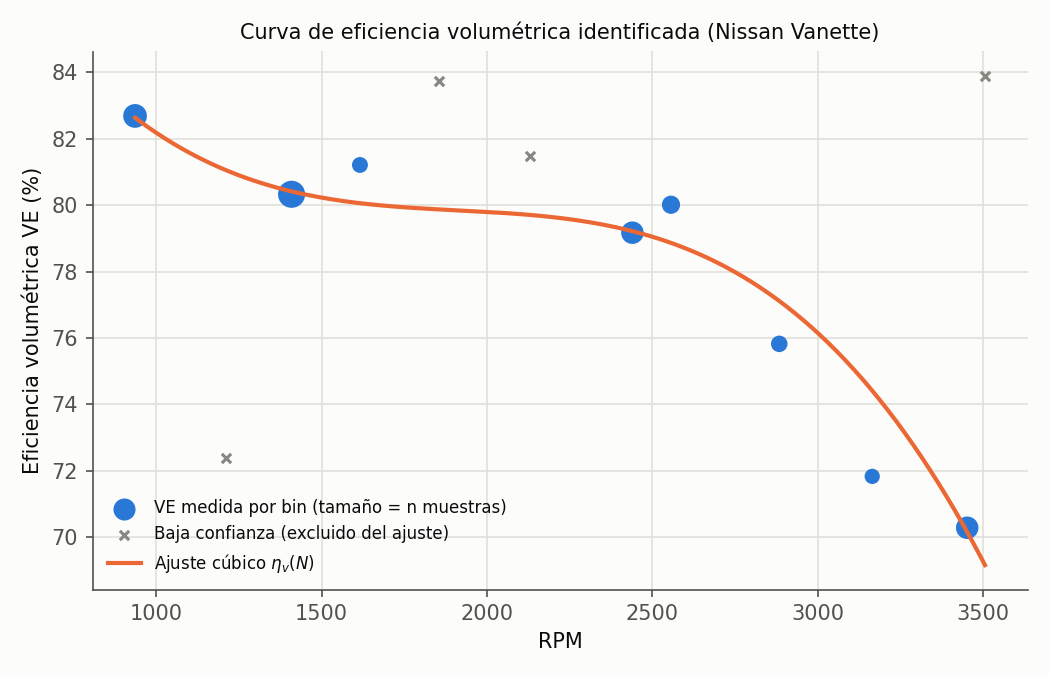
\includegraphics[width=0.8\textwidth]{Images/ve_curve_fit_vanette.png}

	\vspace{2pt}
	{\footnotesize\textit{Nota.} Círculos: VE promedio por bin (tamaño proporcional al número de muestras). Cruces: bins de baja confianza, excluidos del ajuste. Línea: polinomio cúbico ponderado, Ecuación~\eqref{eq:etav-cubica}. Elaboración propia.}
\end{figure}

\paragraph{Caso sin MAF: el Changan Honor.} La Ecuación~\eqref{eq:ve_general}
requiere una referencia real de flujo de aire ($MAF_{ref}$) para despejar la
VE de forma directa; sin ella, RPM, MAP e IAT por sí solos no alcanzan para
aislar esa incógnita. El Changan Honor no soporta el PID 0x10
(Tabla~\ref{tab:pids_verificacion}, Capítulo~4), así que
\texttt{ve\_curve\_calibrator.py} no es aplicable a este vehículo: ninguna
manipulación algebraica sustituye a la referencia real que falta.

El escaneo de PIDs del Changan (Apéndice~O) confirma, sin embargo, que sí
soporta el PID~0x06 (STFT), el PID~0x07 (LTFT) y el PID~0x44 (relación de
equivalencia aire-combustible comandada, usada aquí como indicador de lazo
cerrado). Esa combinación es exactamente la que requiere el
Algoritmo~\ref{alg:etav} ya formalizado en la Sección~\ref{sec:lazo-cerrado}:
en vez de una referencia absoluta de aire, usa el propio ajuste de mezcla
que la ECU ya reporta como señal indirecta de que la VE asumida está mal.
\texttt{CODIGOS/ve\_curve\_calibrator\_indirect.py} implementa una versión
offline de ese algoritmo, análoga en estructura a
\texttt{ve\_curve\_calibrator.py} (mismo agrupamiento por bin, mismo umbral
mínimo de confianza, mismo ajuste cúbico ponderado) pero con un estimador
puntual distinto, el de la Ecuación~\eqref{eq:etav-estimado}:

\begin{equation}
	\hat\eta_v(N) = \eta_v^{0}(N)\left(1 + \frac{\mathrm{STFT}\% + \mathrm{LTFT}\%}{100}\right)
\end{equation}

donde $\eta_v^{0}(N)$ es una curva semilla (por defecto, la misma tabla
genérica de literatura con la que este proyecto arrancó antes de calibrar la
del Vanette, Tabla~\ref{tab:ve_table}, valores originales) y solo se
aceptan muestras con el motor en lazo cerrado ($|\lambda_{cmd}-1|$ dentro de
una tolerancia, PID~0x44), descartando los tramos de enriquecimiento donde
el STFT/LTFT no reflejan un error de VE sino una estrategia distinta de la
ECU. Nótese que esta corrección es multiplicativa y relativa a la curva
semilla (no involucra $V_d$, $P_{MAP}$ ni $T_{IAT}$), a diferencia de la
Ecuación~\eqref{eq:ve_general}, que sí es una inversión absoluta de la
ecuación de gas ideal.

\textit{Advertencia epistemológica.} El resultado de este procedimiento
\textbf{no} debe reportarse como una VE ``calibrada'' del Changan en el mismo
sentido que la del Vanette: es una \emph{corrección relativa a una curva
semilla asumida}, no una medición absoluta. Si la curva semilla generica
está lejos de la realidad de este motor en particular, la corrección
heredará ese sesgo: el método solo garantiza mayor consistencia con los
STFT/LTFT observados, no exactitud absoluta, precisamente por la ausencia de
una referencia real de aire o combustible en este vehículo. Queda, junto con
la recolección misma de los datos con \texttt{CODIGOS/changan\_trim\_logger.py},
como trabajo pendiente para una eventual continuación de este proyecto
(Capítulo~6): no se generó una curva para el Changan dentro del alcance de
este trabajo por no haberse completado esa recolección de campo.

\subsubsection{Calibración contra un tanque real}
\label{sec:calibracion}
No existe forma de que el ESP32 sepa, por sí solo, si el número que calcula
es correcto (no hay con qué comparar dentro del propio microcontrolador).
El procedimiento recomendado: llenar el tanque y anotar el odómetro, manejar
con normalidad hasta la próxima recarga, comparar los litros reales cargados
contra \texttt{trip\_fuel\_L} acumulado en esa misma distancia, y ajustar

\begin{equation}
	\texttt{FUEL\_CALIBRATION\_FACTOR} = \frac{L_{real}}{L_{calculado}}
\end{equation}

en \texttt{config.h}. El criterio de aplicar un único factor multiplicativo
sobre \texttt{fuel\_gs}, en vez de reajustar toda la tabla VE a mano, es que
corrige de forma consistente el instantáneo, el acumulado del viaje y el
costo con un solo número, y es reversible/auditable, a diferencia de
retocar seis puntos de la tabla VE por prueba y error.

% ============================================================
\subsection{Registro en microSD}
% ============================================================

Cada arranque crea un archivo nuevo \texttt{/logs/trip\_NNN.csv} (índice
autoincremental calculado escaneando los archivos existentes, en vez de un
contador separado que podría desincronizarse tras un corte de energía). Se
escribe una fila por segundo, solo después del primer ciclo CAN válido, y se
pausa por completo durante el modo de bajo consumo (Sección~\ref{sec:idle}).

\subsubsection{Por qué CSV}
Se eligió CSV en vez de un formato binario compacto o JSON por fila por tres
razones: es directamente legible/abrible en cualquier hoja de cálculo sin
escribir un parser; el tamaño de fila (unos 100 bytes) es intrascendente
frente a la capacidad de una microSD moderna incluso a una fila por segundo
durante horas; y es el formato que el propio panel web ya necesita poder
descargar y volver a interpretar (Sección~\ref{sec:panelweb}), así que un
mismo formato sirve para ambos usos sin conversión intermedia.



\begin{figure}[H]
	\centering
	\caption{\textit{Fila de ejemplo del CSV (encabezado y fila de datos).}}
	\label{fig:csv_ejemplo}
	\begin{lstlisting}[language=C++, basicstyle=\fontsize{10}{10}\ttfamily, breaklines=true]
uptime_ms,rpm,speed_kmh,map_kpa,iat_c,coolant_c,ve_pct,maf_gs,
fuel_gs,instant_Lh,instant_L100km,trip_km,trip_fuel_L,
trip_avg_L100km,can_status,trip_cost_bs
		
184532,2150,62.0,58.0,29.0,89.0,81.4,7.82,0.532,1.91,3.09,
12.400,0.384,3.10,1,2.67
	\end{lstlisting}
	\begin{minipage}{\linewidth}
		\small
		\textit{Nota.} Estructura del registro de datos almacenado en la tarjeta microSD durante la ejecución del sistema.
	\end{minipage}
\end{figure}

\begin{table}[H]
	\centering
	\captionsetup{labelformat=simple, labelsep=newline, textfont=it, labelfont=bf, justification=raggedright, singlelinecheck=false}
	\caption{Columnas escritas por \texttt{sdLoggerTask} (\texttt{src/sd\_logger.cpp}).}
	\label{tab:columnas_sd_logger}
	\begin{tabular}{ll}
		\toprule
		\rowcolor[rgb]{0.851, 0.851, 0.851}
		Columna & Descripción \\
		\midrule
		\texttt{uptime\_ms}        & Milisegundos desde el arranque \\
		\texttt{rpm}               & Revoluciones por minuto \\
		\texttt{speed\_kmh}        & Velocidad, km/h \\
		\texttt{map\_kpa}          & Presión absoluta del múltiple, kPa \\
		\texttt{iat\_c}            & Temperatura del aire de admisión, °C \\
		\texttt{coolant\_c}        & Temperatura del refrigerante, °C \\
		\texttt{ve\_pct}           & Eficiencia volumétrica usada, \% \\
		\texttt{maf\_gs}           & Flujo másico de aire calculated, g/s \\
		\texttt{fuel\_gs}          & Flujo másico de combustible calculado, g/s \\
		\texttt{instant\_Lh}       & Consumo instantáneo, L/h \\
		\texttt{instant\_L100km}   & Consumo instantáneo, L/100km \\
		\texttt{trip\_km}          & Distancia acumulada del viaje, km \\
		\texttt{trip\_fuel\_L}     & Combustible acumulado del viaje, L \\
		\texttt{trip\_avg\_L100km} & Promedio del viaje, L/100km \\
		\texttt{can\_status}       & Estado del bus CAN (enum \texttt{CanStatus}) \\
		\texttt{trip\_cost\_bs}    & Costo acumulado del viaje, Bs \\
		\bottomrule
	\end{tabular}
	\\
	\vspace{2mm}
	\begin{minipage}{\linewidth}
		\small
		\textit{Nota.} Especificación de la estructura del registro de datos guardado en el archivo CSV de la memoria microSD.
	\end{minipage}
\end{table}
% ============================================================
\subsection{Modo de bajo consumo (``sin contacto'')}
\label{sec:idle}
% ============================================================

\subsubsection{Motivación}
El dispositivo se alimenta del pin 16 del conector OBD2, que entrega
12\,V \textbf{constantes} sin importar la posición de la llave. Si el
firmware siguiera sondeando el bus a ritmo completo, con el panel web y
todos los periféricos encendidos las 24 horas, se convertiría en una carga
parásita permanente sobre la batería del vehículo. La primera versión de
este modo se basaba en detectar RPM$=0$ y solo bajaba el ritmo de sondeo
(una mejora real pero modesta, porque el ESP32-S3 seguía activo con el
WiFi encendido). La versión actual va más lejos: separa la alimentación en
dos rieles y usa \textbf{deep sleep} real del ESP32-S3 mientras no hay
contacto.

\subsubsection{Dos rieles de alimentación}
La PCB entrega dos salidas de 3.3\,V independientes desde el 12\,V
constante del OBD2:

\begin{itemize}
	\item \textbf{Riel 1} (siempre encendido): ESP32-S3 + SN65HVD230. Tiene
	que quedar siempre alimentado porque el transceptor es lo único
	capaz de ``escuchar'' el bus CAN para saber cuándo volvió el
	contacto.
	\item \textbf{Riel 2} (conmutado por software): LEDs + OLED, y por
	separado la microSD. Se corta por completo mientras no hay
	contacto.
\end{itemize}

\subsubsection{Circuito de \textit{power-gating}: MOSFET y pines}
\label{sec:powergate}
Cada riel 2 se controla con un MOSFET de \textbf{canal P, como interruptor
	de alto lado} (corta el 3.3\,V que entra al periférico, no su GND). Se
prefiere sobre un N-MOSFET de bajo lado porque con este último el GND del
periférico puede quedar ligeramente flotante mientras conduce, lo que
genera problemas de integridad de señal en buses referenciados a GND como
I2C (OLED) y SPI (microSD).

\begin{table}[H]
	\centering
	\captionsetup{labelformat=simple, labelsep=newline, textfont=it, labelfont=bf, justification=raggedright, singlelinecheck=false}
	\caption{Pines de \textit{power-gating}, \texttt{include/config.h}.}
	\label{tab:pines_power_gating}
	\begin{tabular}{lll}
		\toprule
		\rowcolor[rgb]{0.851, 0.851, 0.851}
		Señal & GPIO ESP32-S3 & Controla \\
		\midrule
		\texttt{PIN\_PWR\_LED\_OLED} & GPIO6 & LEDs + OLED \\
		\texttt{PIN\_PWR\_SD}       & GPIO7 & microSD \\
		\bottomrule
	\end{tabular}
	\\
	\vspace{2mm}
	\begin{minipage}{\linewidth}
		\small
		\textit{Nota.} Asignación de los pines de salida del microcontrolador utilizados para conmutar la alimentación de los periféricos durante los modos de bajo consumo.
	\end{minipage}
\end{table}

Ambos GPIO son de dominio RTC en el ESP32-S3 (rango GPIO0-21), requisito
para que \texttt{gpio\_hold\_en()} pueda retener su nivel lógico durante el
\textit{deep sleep} \citep{espressif2024trm}. Topología de cada MOSFET
(misma para los dos rieles):

\begin{figure}[H]
	\centering
	\caption{\textit{Interruptor de alto lado con P-MOSFET, un canal por riel.}}
	\label{fig:pmosfet_switch}
	\begin{lstlisting}[language=C++, basicstyle=\fontsize{10}{10}\ttfamily, breaklines=true]
Riel 2 (3.3V) ---+--------------------- Source (P-MOSFET)
|
[R_pullup ~10k]
|
GPIO --[R_gate ~1k]------------------- Gate
|
Drain --- carga (OLED+LED, o microSD)
	\end{lstlisting}
	\begin{minipage}{\linewidth}
		\small
		\textit{Nota.} Esquema básico del circuito de conmutación en el lado alto para el control de energía de periféricos.
	\end{minipage}
\end{figure}

El criterio detrás de cada componente: como el GPIO y el riel 2 comparten
el mismo nivel lógico (3.3\,V), no hace falta un transistor adicional para
manejar la compuerta: GPIO en alto da $V_{gs}=0$ (MOSFET apagado); GPIO en
bajo da $V_{gs}\approx-3.3\,\text{V}$, muy por debajo del umbral típico de
un P-MOSFET de nivel lógico ($-1$ a $-2\,\text{V}$ aprox., p.\,ej. un
AO3401A o equivalente). La resistencia de \textit{pull-up} en la
compuerta asegura que el MOSFET arranque apagado por defecto durante el
breve instante antes de que el firmware configure el GPIO como salida; la
resistencia en serie hacia el GPIO limita la corriente de carga de la
compuerta.

\subsubsection{Cadena de regulación}
\label{sec:regchain}
La alimentación completa, del 12\,V del OBD2 a los dos rieles de 3.3\,V,
pasa por tres reguladores en cascada:

\begin{enumerate}
	\item \textbf{TPS54302}: convertidor \textit{buck} (conmutado) que baja
	el 12\,V del pin 16 a 5\,V. Es la única etapa de conversión
	conmutada del sistema; las dos siguientes son lineales.
	\item \textbf{AMS1117} (5\,V $\rightarrow$ 3.3\,V): alimenta el
	\textbf{riel 1} (ESP32-S3 + SN65HVD230). Nunca se apaga.
	\item \textbf{AP2112} (5\,V $\rightarrow$ 3.3\,V): alimenta el
	\textbf{riel 2}; su salida de 3.3\,V entra a los dos MOSFET de la
	Sección~\ref{sec:powergate}, que gatean OLED+LED y microSD por
	separado. El AP2112 en sí mismo nunca se apaga (solo se corta lo
	que hay \textit{después} de los MOSFET), pero al ser una LDO de
	muy baja corriente de reposo su aporte al consumo en espera es
	pequeño de todos modos (Sección~\ref{sec:consumo}).
\end{enumerate}

Esta cadena (\textit{buck} + 2 LDO en paralelo desde el mismo 5\,V) es una
elección de diseño válida y común, pero tiene una consecuencia directa para
el consumo ``sin contacto'' que conviene tener presente: a diferencia del
AP2112, el \textbf{AMS1117 es una LDO de propósito general, no de bajo
	consumo}: su corriente de reposo (\textit{ground current}) es
comparativamente alta, típicamente 5-8\,mA casi sin importar la carga en
su salida, con variación notable entre fabricantes clon del mismo chip.
Como el AMS1117 alimenta justo el riel que nunca se apaga, esa corriente de
reposo se sostiene las 24\,horas del día, se detalla en la
Sección~\ref{sec:consumo}.

\subsubsection{Implementación en firmware}
\texttt{canObd2CheckContact()} manda un único \textit{ping} (PID
\texttt{0x0C}, RPM, obligatorio en todo ECU OBD2) y reporta si algo
respondió, sin importar el valor. Se usa en dos puntos:

\begin{itemize}
	\item Al arrancar (\texttt{setup()}, tanto en un encendido normal como al
	despertar del \textit{deep sleep}): si no hay contacto, el chip
	vuelve a dormir antes de tocar el riel 2 o el WiFi.
	\item Ya despierto, dentro de \texttt{canObd2Task}: si el bus deja de
	responder durante \texttt{CONTACT\_LOST\_DEBOUNCE\_CYCLES} ciclos
	seguidos (3, para no dormirse por un solo \textit{frame} perdido en
	un bus ocupado), se considera que se fue el contacto.
\end{itemize}

\begin{figure}[H]
	\centering
	\caption{\textit{Entrada a deep sleep, \texttt{src/power\_sleep.cpp}.}}
	\label{fig:deepsleep}
	\begin{lstlisting}[language=C++, basicstyle=\fontsize{10}{10}\ttfamily, breaklines=true]
void enterDeepSleepUntilContact() {
	sdLoggerShutdown();  // cierra el archivo antes de cortarle la energia
	WiFi.mode(WIFI_OFF);
			
	powerGateSet(false);
	gpio_hold_en((gpio_num_t)PIN_PWR_LED_OLED);
	gpio_hold_en((gpio_num_t)PIN_PWR_SD);
	gpio_deep_sleep_hold_en(); // sin esto el hold no sobrevive al deep sleep
			
	esp_sleep_enable_timer_wakeup(DEEP_SLEEP_WAKE_INTERVAL_US);
	esp_deep_sleep_start();  // no retorna
}
	\end{lstlisting}
	\begin{minipage}{\linewidth}
		\small
		\textit{Nota.} Procedimiento para el apague seguro de perifericos, mantenimiento del estado GPIO (hold) y entrada al modo de bajo consumo deep sleep en el ESP32.
	\end{minipage}
\end{figure}

Cerrar el archivo de la SD \textbf{antes} de cortar su MOSFET es
obligatorio, no una formalidad: cortar la alimentación con un archivo
abierto arriesga corromper el sistema de archivos completo, no solo perder
la última fila. El \textit{deep sleep} borra toda la RAM salvo el dominio
RTC, así que al despertar \texttt{setup()} vuelve a correr desde el
principio, exactamente como un arranque en frío.

\subsubsection{Consumo estimado y autonomía de la batería}
\label{sec:consumo}
Los siguientes números son estimaciones a partir de valores típicos de
hoja de datos, no mediciones sobre la placa real (sirven para tener una
idea de orden de magnitud, no un valor exacto).

\begin{table}[H]
	\centering
	\small
	\captionsetup{labelformat=simple, labelsep=newline, textfont=it, labelfont=bf, justification=raggedright, singlelinecheck=false}
	\caption{Contribuyentes al consumo promedio ``sin contacto'', cadena real (TPS54302 + AMS1117 + AP2112).}
	\label{tab:consumo_sin_contacto}
	\begin{tabular}{p{2.2cm}p{4.0cm}p{2.2cm}p{4.5cm}}
		\toprule
		\rowcolor[rgb]{0.851, 0.851, 0.851}
		Nodo & Fuente & Aporte típico & Nota \\
		\midrule
		3.3~V (riel 1) & ESP32-S3 en deep sleep & $\sim$0.02~mA & 10–25~$\mu$A \citep{espressif2024datasheet} \\
		3.3~V (riel 1) & SN65HVD230, siempre activo & $\sim$5–10~mA & Modo normal, no standby \citep{sn65hvd230_datasheet} \\
		3.3~V (riel 1) & Pulsos de despertar (cada 20~s) & $\sim$1.5–2~mA & Promediado: $\sim$150~mA por $\sim$0.2–0.3~s \\
		5~V & \textbf{AMS1117}, corriente de reposo propia & \textbf{$\sim$5–8~mA} & Casi independiente de la carga \\
		5~V & AP2112, corriente de reposo propia & $\sim$0.06~mA & Sin carga (MOSFET de salida abiertos) \\
		12~V & TPS54302, corriente de reposo propia & $\sim$0.1–0.3~mA & \\
		\midrule
		\multicolumn{2}{l}{\textbf{Total aproximado, lado 12~V}} & \textbf{$\sim$7–9~mA} & Ver conversión abajo \\
		\bottomrule
	\end{tabular}
	\vspace{2mm}
	\begin{minipage}{\linewidth}
		\small
		\textit{Nota.} Estimación del consumo de corriente del sistema en estado de reposo (sin contacto de encendido), detallando la contribución de cada componente regulador y periférico en la línea de alimentación.
	\end{minipage}
\end{table}

El resultado es contraintuitivo pero importante: \textbf{el transceptor CAN
	y la LDO del riel 1, no el ESP32-S3, dominan el consumo mientras el
	dispositivo ``duerme''}: ese riel no se puede cortar sin perder la
capacidad de detectar cuándo vuelve el contacto (Sección~\ref{sec:powergate}).
El \textit{deep sleep} resuelve la parte del ESP32-S3 casi por completo,
pero no puede resolver la del transceptor ni la de su LDO con esta
arquitectura de dos rieles fija.

Convertir la corriente del lado 3.3\,V/5\,V al lado 12\,V: el AMS1117 y el
AP2112 son LDO (no reducen corriente, solo voltaje, disipando la diferencia
como calor), así que la corriente que el TPS54302 debe entregar en su
salida de 5\,V es aproximadamente la suma de lo que consumen el riel 1
completo ($\sim$8.5\,mA de ESP32+SN65+pulsos) más la corriente de reposo
propia del AMS1117 ($\sim$6.5\,mA punto medio) y del AP2112
($\sim$0.06\,mA): $\approx$15\,mA a 5\,V. El TPS54302, al ser un
\textit{buck} conmutado, sí convierte potencia de forma más eficiente
($\sim$80\,\% en carga liviana, estimado):

\begin{equation}
	I_{12V} \approx \frac{5\,\text{V} \times 15\,\text{mA}}{12\,\text{V} \times 0.80} + 0.2\,\text{mA (I}_q\text{ TPS54302)} \approx 8\,\text{mA}
	\label{eq:i12v_reposo}
\end{equation}

Tomando esos $\sim$8\,mA y una batería típica de auto de 50\,Ah (de la cual,
por buena práctica, no conviene usar más del 50\,\% para no acortar su vida
útil, es decir $\sim$25\,000\,mAh utilizables):

\begin{equation}
	\frac{25\,000\,\text{mAh}}{8\,\text{mA}} \approx 3\,125\,\text{horas} \approx 130\,\text{días}
\end{equation}

Es decir, \textbf{el dispositivo por sí solo} tardaría del orden de 4-5
meses en consumir la mitad de una batería sana (menos que si el riel 1
usara una LDO de baja corriente de reposo en vez del AMS1117, pero todavía
un margen amplio frente al uso normal del vehículo). En la práctica esto
importa menos de lo que parece, porque el propio vehículo ya tiene su
propio consumo parásito de fábrica (alarma, memorias de radio/ECU, reloj,
etc.), típicamente $\sim$20-50\,mA con todo ``apagado'' (del mismo orden o
mayor que el aporte de este dispositivo), y ese consumo de base es el que
realmente determina cuánto aguanta la batería estacionada, con o sin el
ESP32-S3 conectado.

\textbf{Decisión de diseño:} se evaluó reemplazar el AMS1117 del riel 1 por
una LDO de baja corriente de reposo (el propio AP2112, un MCP1700, o una
TPS7A02 con $I_q$ en el orden de nanoamperios bajarían el consumo "sin
contacto" varios mA más), pero se optó por mantener el AMS1117 y el AP2112
tal como estaban ya elegidos en la placa: es el contribuyente individual
más grande después del SN65HVD230, y queda documentado aquí como una
compensación consciente entre simplicidad/costo de la lista de materiales y
la autonomía teórica de la batería, no un descuido.

\subsubsection{Consumo estimado en modo activo}
\label{sec:consumo_activo}

El mismo procedimiento de conversión de la Ecuación~\eqref{eq:i12v_reposo} se
aplica a dos escenarios activos, con la diferencia de que en modo activo la
corriente que domina en cada riel ya no es la de reposo de las LDO sino la
carga real que atraviesan (el AMS1117 y el AP2112 no reducen corriente,
solo la dejan pasar con caída de tensión). Los aportes por componente:

\begin{itemize}
	\item \textbf{ESP32-S3, activo con WiFi asociado (modo \textit{modem-sleep},
	tráfico intermitente cada 500\,ms, no transmisión continua):}
	$\sim$40--48\,mA a 240\,MHz \citep{espressif2024datasheet}. Es el escenario
	realista del panel web: el WiFi permanece asociado pero la radio pasa la
	mayor parte del tiempo en reposo entre los envíos periódicos del
	WebSocket, muy distinto del pico de $>$283\,mA que exige una transmisión
	continua a máxima tasa \citep{espressif2024datasheet}.
	\item \textbf{ESP32-S3, activo sin WiFi (CPU corriendo, radio apagada):}
	no tabulado directamente en la hoja de datos; se estima $\sim$25\,mA,
	por debajo del modo \textit{modem-sleep} al no incluir el consumo
	periódico de la banda base Wi-Fi.
	\item \textbf{SN65HVD230, activo:} $\sim$8\,mA, punto medio del rango ya
	usado en la Tabla~\ref{tab:consumo_sin_contacto} \citep{sn65hvd230_datasheet}.
	\item \textbf{OLED SSD1306, encendida:} $\sim$15\,mA, punto medio de
	10--20\,mA \citep{solomon2008ssd1306}.
	\item \textbf{MicroSD, activa (lectura/escritura):} $\sim$25\,mA, valor
	típico de fabricante para tarjetas microSD en operación (no corresponde a
	una hoja de datos de un modelo específico, a diferencia de los aportes
	anteriores).
\end{itemize}

\begin{table}[H]
	\centering
	\small
	\captionsetup{labelformat=simple, labelsep=newline, textfont=it, labelfont=bf, justification=raggedright, singlelinecheck=false}
	\caption{Consumo estimado en modo activo, dos escenarios (misma cadena TPS54302+AMS1117+AP2112)}
	\label{tab:consumo_activo}
	\begin{tabular}{p{5.5cm}p{3cm}p{3cm}}
		\toprule
		\rowcolor[rgb]{0.851, 0.851, 0.851}
		Escenario & Riel 1+2 a 5\,V & $I_{12V}$ estimada \\
		\midrule
		Activo, WiFi + OLED + microSD & $\sim$100\,mA & $\sim$52\,mA \\
		Activo, solo CAN + microSD (sin WiFi ni OLED) & $\sim$65\,mA & $\sim$34\,mA \\
		\bottomrule
	\end{tabular}
	\vspace{2mm}
	\begin{minipage}{\linewidth}
		\small
		\textit{Nota.} $I_{12V}$ calculada con la Ecuación~\eqref{eq:i12v_reposo} (eficiencia del TPS54302 $\sim$80\,\%), sumando los aportes de componente listados arriba más la corriente de reposo propia de cada LDO. Son estimaciones de orden de magnitud, no mediciones, pendientes de validar una vez ensamblada la PCB (Sección~4.3.8 del Capítulo~4).
	\end{minipage}
\end{table}

\subsubsection{Recomendación de mantenimiento}
Con esos números, la recomendación práctica no cambia mucho respecto al
cuidado normal de cualquier batería de auto: \textbf{arrancar/circular el
	vehículo al menos cada 2-3 semanas}, o usar un cargador de mantenimiento
(\textit{battery tender}) si va a quedar estacionado más tiempo que eso.
Con la cadena de reguladores actual (AMS1117 incluido) el dispositivo
agrega una fracción del consumo parásito que el auto ya tiene de fábrica
(notable, pero no dominante), así que este intervalo sigue siendo una
recomendación razonable sin necesitar ser más estricta.

\subsubsection{¿Afecta consultar tan seguido?}
Con la arquitectura actual hay dos frecuencias distintas que vale la pena
separar:

\begin{itemize}
	\item \textbf{Sondeo CAN mientras hay contacto} (un ciclo completo de 8
	PIDs cada $\sim$0.2-1.4\,s): el bus CAN a 500\,kbit/s tiene
	capacidad de sobra para esto (cada trama de petición/respuesta son
	unos 100 bits, así que incluso varias por segundo representan bien
	menos del 1\,\% del ancho de banda del bus). Una ECU real está
	diseñada para atender consultas de diagnóstico bastante más
	frecuentes que esto sin ningún problema; no hay riesgo de saturar
	el bus ni de sobrecargar la ECU.
	\item \textbf{Escritura a la microSD, una fila por segundo}
	(\texttt{SD\_LOG\_INTERVAL\_MS}): las escrituras son secuenciales
	(se van agregando al final del archivo, no se reescribe una y otra
	vez el mismo bloque), que es el mejor caso posible para el
	desgaste de la memoria flash. Una fila ronda los 100 bytes; a una
	por segundo son unos 360\,KB por hora de viaje, insignificante
	frente a la resistencia típica de una microSD moderna (miles de
	ciclos de escritura por bloque, con \textit{wear leveling}
	integrado). No es un factor de desgaste relevante en la práctica.
\end{itemize}

% ============================================================
\subsection{Panel web}
\label{sec:panelweb}
% ============================================================

\subsubsection{Punto de acceso WiFi: por qué SoftAP en vez de solo STA}
El dispositivo siempre levanta su propio punto de acceso (SSID
\texttt{ESP32\_OBD2}, IP típica \texttt{192.168.4.1}) en vez de depender
únicamente de unirse a una red WiFi conocida. El criterio es el contexto de
uso real: dentro de un vehículo casi nunca hay una red WiFi conocida en
rango, así que un diseño solo-STA dejaría el panel inaccesible la mayor
parte del tiempo. El SoftAP garantiza acceso local sin esa dependencia;
unirse además como cliente a una red conocida queda como algo opcional,
únicamente para sincronizar hora por NTP cuando hay una disponible.

\subsubsection{Por qué ESPAsyncWebServer en vez del servidor síncrono de Arduino}
Se eligió ESPAsyncWebServer \citep{espasyncwebserver2024} sobre el
\texttt{WebServer} síncrono incluido en el core de Arduino-ESP32 porque
atiende las conexiones de forma asíncrona, basada en eventos: una petición
lenta (por ejemplo, una descarga de CSV grande) no bloquea el hilo mientras
espera que el cliente reciba los datos. Dado que el servidor corre en el
mismo núcleo que la pila WiFi (Sección~\ref{sec:herramientas}), un modelo
síncrono habría significado que una descarga lenta retrasara también el
resto del tráfico de red, incluyendo el WebSocket que empuja los datos en
vivo.

\subsubsection{Empuje en vivo: WebSocket con respaldo por \textit{polling}}
El estado se empuja a los clientes por WebSocket cada 500\,ms
(la Figura~\ref{fig:merge} ya mostró de dónde sale ese dato), con un
mecanismo de respaldo: si el navegador detecta que el WebSocket no está
abierto, recurre a pedir \texttt{/api/live} por HTTP cada 1.5\,s. El
criterio es la robustez: un WebSocket puede caerse por muchas razones ajenas
al firmware (el navegador durmiendo la pestaña, un cambio de red en el
celular), y el panel no debería quedar congelado solo porque ese canal se
cortó.

\subsubsection{JSON con ArduinoJson}
Las respuestas HTTP y los mensajes WebSocket se serializan con la librería
ArduinoJson \citep{arduinojson2024} en vez de concatenar \textit{strings} a
mano. El criterio: construir JSON por concatenación de texto es una fuente
común de errores de escape/formato difíciles de depurar en un
microcontrolador, mientras que ArduinoJson gestiona el documento en un
búfer de tamaño acotado y conocido, algo relevante en un sistema con 320\,KB
de RAM total repartidos entre cinco tareas.

\begin{table}[H]
	\centering
	\captionsetup{labelformat=simple, labelsep=newline, textfont=it, labelfont=bf, justification=raggedright, singlelinecheck=false}
	\caption{Endpoints servidos por ESPAsyncWebServer (\texttt{src/web\_server.cpp}).}
	\label{tab:web_endpoints}
	\begin{tabular}{lll}
		\toprule
		\rowcolor[rgb]{0.851, 0.851, 0.851}
		Método & Ruta & Descripción \\
		\midrule
		GET  & \texttt{/}            & Panel del dashboard (HTML embebido en el firmware) \\
		WS   & \texttt{/ws}          & WebSocket, empuja el estado en vivo cada 500~ms \\
		GET  & \texttt{/api/live}    & Snapshot JSON del estado actual \\
		GET  & \texttt{/api/files}   & Lista de archivos en \texttt{/logs} \\
		GET  & \texttt{/api/download} & Descarga un CSV completo \\
		GET  & \texttt{/api/chartdata}& Puntos decimados para graficar \\
		POST & \texttt{/api/reset}    & Reinicia el contador de viaje \\
		\bottomrule
	\end{tabular}
	\\
	\vspace{2mm}
	\begin{minipage}{\linewidth}
		\small
		\textit{Nota.} Definición de la interfaz de programación de aplicaciones (API) REST y punto de conexión WebSocket implementados para el servidor web incrustado del microcontrolador.
	\end{minipage}
\end{table}

\subsubsection{Interfaz}
El HTML/CSS/JS está embebido por completo en el firmware, sin dependencias
de CDN externo (criterio directo del contexto de uso: el SoftAP no tiene
salida a internet, así que cualquier librería externa de gráficas
simplemente no cargaría). El panel tiene dos pestañas (\textit{En vivo} e
\textit{Historial}), tarjetas destacadas con el consumo instantáneo,
litros y costo del viaje, casillas para elegir qué variables graficar, y un
\textit{tooltip} interactivo con línea guía. Cuando hay 2 o más variables
seleccionadas a la vez, cada una se normaliza a su propio rango (0-100\,\%)
para poder comparar formas de curva con unidades muy distintas (RPM 0-7000
frente a L/100km 0-20) sin que una aplaste visualmente a la otra.

% ============================================================
\subsection{Compilación y programación}
\label{sec:build}
% ============================================================

\subsubsection{PlatformIO}

\begin{figure}[H]
	\centering
	\caption{\textit{Configuración relevante de \texttt{platformio.ini}.}}
	\label{fig:platformio_config}
	\begin{lstlisting}[language=C++, basicstyle=\fontsize{10}{10}\ttfamily, breaklines=true]
board = esp32-s3-devkitc-1
board_build.flash_mode = qio
board_build.arduino.memory_type = qio_opi
board_build.psram_type = opi
board_upload.flash_size = 16MB
	\end{lstlisting}
	\begin{minipage}{\linewidth}
		\small
		\textit{Nota.} Parámetros de compilación y definición del tipo de memoria Flash y PSRAM OPI para el módulo ESP32-S3.
	\end{minipage}
\end{figure}

\texttt{platformio.ini} define un entorno de compilación por vehículo
(\texttt{[env:vanette]} / \texttt{[env:changan]}) en vez de un único
firmware genérico: cada uno agrega un \textit{build flag}
(\texttt{-DVEHICLE\_VANETTE} / \texttt{-DVEHICLE\_CHANGAN}) que
selecciona en tiempo de compilación, mediante bloques
\texttt{\#if}/\texttt{\#elif} en \texttt{config.h} y
\texttt{fuel\_calc.cpp}, la cilindrada real y la tabla VE
correspondientes a cada motor (Sección~\ref{sec:ve-general}). El criterio
de resolver esto en tiempo de compilación, y no dejarlo como una
constante a editar a mano antes de cada \textit{flasheo}, es que un error
de este tipo ya ocurrió una vez en este proyecto (la cilindrada del
Vanette quedó en 1,6\,L en vez de 1,626\,L) y un \textit{build} que no
selecciona ningún vehículo simplemente no compila (\texttt{\#error}), en
vez de compilar en silencio con un valor incorrecto. Para compilar y
subir: \texttt{pio run -e vanette -t upload} o
\texttt{pio run -e changan -t upload}, y luego
\texttt{pio device monitor -b 115200}.

\subsubsection{USB nativo frente a UART externo}
El \textit{devkit} de desarrollo solo expone el \textbf{USB nativo} del
ESP32-S3 (el periférico USB-Serial-JTAG integrado, sin un chip puente
CP2102/CH340 aparte). Esto tiene dos implicancias para una PCB propia:

\begin{enumerate}
	\item Programar por UART \textbf{siempre funciona}, sin importar la
	configuración del firmware: \texttt{esptool} habla directo con el
	\textit{bootloader} de ROM del chip, independiente de cualquier
	opción de compilación de la aplicación.
	\item El firmware define \texttt{-DARDUINO\_USB\_CDC\_ON\_BOOT=1}. Con ese
	\textit{flag}, el objeto \texttt{Serial} de Arduino se enruta al
	USB nativo en vez del UART0 físico (GPIO43/44). Si la PCB propia usa
	un adaptador UART externo y no tiene el USB nativo conectado a
	nada, ese \textit{flag} debe quitarse: de lo contrario el monitor
	serie del adaptador UART no mostrará nada, aunque el firmware esté
	corriendo correctamente.
\end{enumerate}

\subsubsection{Circuito mínimo para programar/arrancar}
Cualquier placa propia con el ESP32-S3 necesita, como mínimo: \texttt{EN}
(reset) con \textit{pull-up} a 3.3\,V y un capacitor de $\sim$1\,$\mu$F a
GND; \texttt{GPIO0} (BOOT) con \textit{pull-up} a 3.3\,V y un botón a GND
para forzar el modo \textit{bootloader} manualmente; y, opcionalmente, un
circuito de auto-reset (2 transistores desde DTR/RTS del adaptador UART
hacia EN y GPIO0) para que PlatformIO entre solo al modo de programación sin
botones.

% ============================================================
\subsection{Solución de problemas comunes}
% ============================================================

\begin{itemize}
	\item \textbf{La subida se queda en ``Connecting...'' indefinidamente.}
	Entrar manualmente en modo \textit{bootloader} (mantener BOOT,
	pulsar y soltar RESET/EN, soltar BOOT, y recién ahí lanzar la
	subida). Verificar también que ningún otro programa tenga el
	puerto COM abierto.
	\item \textbf{El monitor serie no muestra nada tras programar.} Revisar
	que \texttt{ARDUINO\_USB\_CDC\_ON\_BOOT} coincida con el hardware
	real (Sección~\ref{sec:build}).
	\item \textbf{\texttt{sdSelectCard(): Select Failed} / \texttt{SD=0} en el
		arranque.} Casi siempre es cableado/alimentación: revisar tarjeta
	insertada, tensión correcta del módulo lector, continuidad de los 4
	pines SPI + GND, formato FAT32, y el \textit{pull-up} de
	10\,k$\Omega$ en CS si se soldó directo sin módulo.
	\item \textbf{El panel web no carga en el celular.} Escribir
	\texttt{http://192.168.4.1} con el esquema explícito (varios
	navegadores intentan \texttt{https://} por defecto y el dispositivo
	no tiene TLS). Algunos celulares además desconectan una red WiFi
	sin salida a internet a menos que se les indique quedarse
	conectados igual.
\end{itemize}


%El sistema migró de una arquitectura distribuida en dos microcontroladores
%(ATmega328P con controlador CAN externo MCP2515 y un ESP32-C3 dedicado a la
%interfaz web, enlazados por UART) a una arquitectura monolítica sobre un único
%ESP32, que incorpora controlador CAN nativo (TWAI) y conectividad Wi-Fi en el mismo
%encapsulado. Esta consolidación elimina el enlace UART entre microcontroladores ---y
%con él la necesidad de una verificación de integridad CRC-8 a nivel de
%aplicación, pues el bus CAN ya provee un CRC de 15 bits implementado en
%hardware--- y permite explotar los \textbf{dos núcleos del ESP32} mediante el
%planificador en tiempo real FreeRTOS \citep{barry2016freertos}. La presente sección
%detalla el diseño del firmware organizándolo en cuatro subsistemas ---adquisición,
%procesamiento, almacenamiento y visualización--- y cierra con el análisis de tiempos
%de respuesta y la estrategia de robustez.

%% ---------------------------------------------------------------------
%\subsection{Arquitectura de firmware del ESP32}
%\label{subsec:arq-firmware}
%
%\subsubsection{Modelo de concurrencia sobre dos núcleos}
%
%El ESP32 dispone de dos núcleos de procesamiento. El firmware asigna a cada uno
%tareas con requisitos temporales distintos, evitando que las operaciones bloqueantes
%de red interfieran con la adquisición determinista del bus CAN. La
%Tabla~\ref{tab:tareas} resume las tareas FreeRTOS, su núcleo y su prioridad.
%
%\begin{table}[htbp]
%	\captionsetup{labelformat=simple, labelsep=newline, textfont=it, labelfont=bf, justification=raggedright, singlelinecheck=false}
%	
%	\caption{Tareas FreeRTOS, asignación de núcleo y prioridad.}
%	\centering
%	\label{tab:tareas}
%	\begin{tabular}{@{}lcccl@{}}
%		\toprule
%		\rowcolor[rgb]{0.851, 0.851, 0.851}
%		\textbf{Tarea} & \textbf{Núcleo} & \textbf{Prioridad} & \textbf{Periodo} & \textbf{Función} \\
%		\midrule
%		\texttt{taskAcq} & 1 & 5 (alta)  & 250 ms & Adquisición OBD-II + cálculo \\
%		\texttt{taskLog} & 1 & 2 (media) & evento & Registro en MicroSD \\
%		\texttt{taskWeb} & 0 & 3 (media) & 200 ms & Servidor Wi-Fi + WebSocket \\
%		\bottomrule
%	\end{tabular}
%	
%	\vspace{2pt}
%	{\footnotesize\textit{Nota.} Elaboración propia.}
%\end{table}
%
%La comunicación entre tareas emplea dos mecanismos: una \emph{cola} (FreeRTOS queue)
%desde la adquisición hacia el registro en disco, y una \emph{estructura compartida}
%protegida por sección crítica para el último valor publicado a la web. La
%Figura~\ref{fig:arq-tareas} ilustra la arquitectura.
%
%\begin{figure}[H]
%	% Formato APA 7
%	\captionsetup{labelformat=simple, labelsep=newline, textfont=it, labelfont=bf, justification=raggedright, singlelinecheck=false}
%	\caption[Arquitectura de tareas concurrentes del firmware]{Arquitectura de tareas concurrentes del firmware del sistema embebido.}
%	\label{fig:arq-tareas}
%	\centering
%	
%	\vspace{4mm}
%	\resizebox{0.95\textwidth}{!}{% Se redujo la agresividad del escalado haciendo el dibujo más compacto
%		\begin{tikzpicture}[
%			font=\normalsize,
%			task1/.style={rectangle, draw=blue!75!black, line width=0.7pt, rounded corners,
%				align=center, minimum height=1.3cm, minimum width=2.7cm, fill=blue!10},
%			task0/.style={rectangle, draw=teal!75!black, line width=0.7pt, rounded corners,
%				align=center, minimum height=1.3cm, minimum width=2.7cm, fill=teal!10},
%			store/.style={cylinder, shape border rotate=90, draw=orange!85!black, line width=0.7pt,
%				aspect=0.3, minimum height=1.5cm, minimum width=1.8cm, align=center,
%				fill=orange!15},
%			busn/.style={rectangle, draw=violet!75!black, line width=0.7pt, rounded corners,
%				align=center, minimum height=1.2cm, minimum width=2.0cm, fill=violet!10},
%			cli/.style={rectangle, draw=gray!80!black, line width=0.7pt, rounded corners,
%				align=center, minimum height=1.3cm, minimum width=2.2cm, fill=black!5},
%			reg1/.style={rectangle, draw=blue!60, dashed, line width=0.9pt, rounded corners,
%				inner sep=14pt, fill=blue!3},
%			reg0/.style={rectangle, draw=teal!60, dashed, line width=0.9pt, rounded corners,
%				inner sep=14pt, fill=teal!3},
%			line/.style={-{Latex[length=2.6mm]}, line width=1.0pt, draw=black!75},
%			lbl/.style={font=\small, fill=white, inner sep=2pt, align=center}
%			]
%			
%			% 1. Tareas y periferia (Distancias reducidas para evitar miniaturización)
%			\node[task1] (acq) {\texttt{taskAcq}\\[2pt]\footnotesize adquisición + cálculo};
%			\node[task1, below=1.8cm of acq] (log) {\texttt{taskLog}\\[2pt]\footnotesize registro SD};
%			\node[task0, right=3.5cm of acq] (web) {\texttt{taskWeb}\\[2pt]\footnotesize Wi-Fi + WebSocket};
%			
%			\node[busn, left=1.5cm of acq] (can) {Bus CAN};
%			\node[store, left=1.5cm of log] (sd) {Micro SD};
%			\node[cli, right=1.5cm of web] (cli) {Navegador\\[2pt]\footnotesize (Cliente)};
%			
%			% 2. Regiones de nucleo (capa de fondo)
%			\begin{scope}[on background layer]
%				\node[reg1, fit=(acq)(log)] (region1) {};
%				\node[reg0, fit=(web)] (region0) {};
%			\end{scope}
%			
%			% Títulos de los núcleos
%			\node[above=2mm of region1, font=\bfseries, text=blue!75!black] {Núcleo 1 (Tiempo Real)};
%			\node[above=2mm of region0, font=\bfseries, text=teal!75!black] {Núcleo 0 (Red)};
%			
%			% 3. Conexiones
%			\draw[line] (can) -- (acq);
%			\draw[line] (acq) -- node[lbl, right] {Cola\\(Queue)} (log);
%			\draw[line] (log) -- (sd);
%			\draw[line] (acq) -- node[lbl] {Estructura\\compartida} (web);
%			\draw[line] (web) -- node[lbl, above] {JSON\\(WS)} (cli);
%			
%		\end{tikzpicture}%
%	}
%	
%	\vspace{4mm}
%	\small\raggedright
%	\textit{Nota.} Elaboración propia. La adquisición de datos y el cálculo iterativo se ejecutan en el núcleo de tiempo real; mientras que el servidor Wi-Fi y el protocolo WebSocket operan en el núcleo de red, garantizando el aislamiento de tareas críticas y previniendo bloqueos durante la lectura del bus OBD-II.
%\end{figure}
%\subsubsection{Máquina de estados de adquisición}
%
%La tarea \texttt{taskAcq} implementa una máquina de estados finita (FSM) que se
%recorre una vez por periodo: \texttt{INIT} (configuración del controlador TWAI),
%\texttt{REQUEST} (envío de la petición de un PID), \texttt{WAIT} (espera de respuesta
%con tiempo límite), \texttt{PROCESS} (decodificación y cálculo de consumo) y
%\texttt{LOG} (encolado para registro). La Figura~\ref{fig:fsm-sw} muestra la
%transición de estados.
%
%\begin{figure}[H]
%	% Formato APA 7
%	\captionsetup{labelformat=simple, labelsep=newline, textfont=it, labelfont=bf, justification=raggedright, singlelinecheck=false}
%	\caption[Máquina de estados de la tarea de adquisición]{Máquina de estados de la tarea de adquisición en el sistema embebido.}
%	\label{fig:fsm-sw}
%	\centering
%	
%	\vspace{4mm}
%	\begin{tikzpicture}[
%		font=\small, 
%		node distance=2.2cm and 1.8cm, % Ligeramente ampliado para evitar amontonamiento
%		st/.style={rectangle, draw, rounded corners, thick, align=center,
%			minimum height=0.85cm, minimum width=1.8cm},
%		line/.style={-{Latex[length=2mm]}, thick}
%		]
%		
%		% 1. Nodos con paleta de colores profesional (suaves para contraste)
%		\node[st, fill=gray!20]   (init) {INIT};
%		\node[st, fill=blue!15, right=of init] (req) {REQUEST};
%		\node[st, fill=orange!20, right=of req] (wait) {WAIT};
%		\node[st, fill=green!15, below=of wait] (proc) {PROCESS};
%		\node[st, fill=purple!15, left=of proc] (log) {LOG};
%		
%		% 2. Conexiones de flujo principal
%		\draw[line] (init) -- (req);
%		\draw[line] (req) -- node[above]{tx} (wait);
%		\draw[line] (wait) -- node[right]{rx ok} (proc);
%		\draw[line] (proc) -- (log);
%		
%		% 3. Retornos y lazos (Corregidos para no chocar)
%		% El retorno de LOG a REQUEST va directo hacia arriba (norte a sur)
%		\draw[line] (log.north) -- node[left]{siguiente PID} (req.south);
%		
%		% El lazo de WAIT a REQUEST forma un arco limpio por la parte superior
%		\draw[line] (wait.north) to[bend right=35] node[above]{timeout} (req.north);
%		
%	\end{tikzpicture}
%	
%	\vspace{4mm}
%	\small\raggedright
%	\textit{Nota.} Elaboración propia. El estado \texttt{LOG} reinicia el ciclo para el siguiente PID; un tiempo límite en el estado \texttt{WAIT} descarta la trama y la máquina continúa su operación.
%\end{figure}
%
%La Figura~\ref{fig:cod-tasks} muestra la creación de las tareas y de la cola, con anclado
%explícito a cada núcleo.
%
%\begin{figure}[H]
%	\caption{Creación de tareas FreeRTOS y cola de registro.}
%	\label{fig:cod-tasks}
%	\begin{lstlisting}[language=C++]
%QueueHandle_t qLog;             // cola adquisicion -> registro
%TelemetrySample gLatest;       // ultimo valor para la web
%portMUX_TYPE   gMux = portMUX_INITIALIZER_UNLOCKED;
%		
%void setup() {
%	canInit();                // controlador TWAI a 500 kbps
%	sdInit();            // MicroSD + carga de tabla eta_v y K
%	qLog = xQueueCreate(32, sizeof(TelemetrySample));
%// adquisicion en nucleo 1 (tiempo real), web en nucleo 0 (red)
%	xTaskCreatePinnedToCore(taskAcq,"acq",8192,NULL,5,NULL,1);
%	xTaskCreatePinnedToCore(taskLog,"log",4096,NULL,2,NULL,1);
%	xTaskCreatePinnedToCore(taskWeb,"web",8192,NULL,3,NULL,0);
%}
%void loop() { vTaskDelete(NULL); }  // todo corre en tareas
%	\end{lstlisting}
%\end{figure}
%
%% ---------------------------------------------------------------------
%\subsection{Subsistema de adquisición OBD-II}
%\label{subsec:adquisicion}
%
%\subsubsection{Controlador CAN nativo (TWAI)}
%
%El controlador TWAI del ESP32 se configura a la velocidad estándar del enlace
%OBD-II sobre CAN, 500 kbps (ISO~15765-4), con filtro abierto para
%aceptar las respuestas de la ECU \citep{sae_j1979_2014}. La Figura~\ref{fig:cod-caninit}
%resume la inicialización.
%
%\begin{figure}[H]
%	\caption{Inicializacion del controlador TWAI a 500 kbps.}
%	\label{fig:cod-caninit}
%	\begin{lstlisting}[language=C++]
%#include "driver/twai.h"
%#define CAN_TX GPIO_NUM_5    // ajustar al netlist de la PCB
%#define CAN_RX GPIO_NUM_4
%		
%void canInit() {
%	twai_general_config_t g =
%	TWAI_GENERAL_CONFIG_DEFAULT(CAN_TX,CAN_RX,TWAI_MODE_NORMAL);
%	twai_timing_config_t t = TWAI_TIMING_CONFIG_500KBITS();
%	twai_filter_config_t f = TWAI_FILTER_CONFIG_ACCEPT_ALL();
%	twai_driver_install(&g, &t, &f);
%	twai_start();
%}
%	\end{lstlisting}
%	
%
%\end{figure}
%
%\subsubsection{Petición y respuesta OBD-II}
%
%Una petición OBD-II en modo~01 (datos en vivo) se envía a la dirección funcional
%\texttt{0x7DF}; la ECU responde en el rango \texttt{0x7E8}--\texttt{0x7EF}. El primer
%byte indica el número de bytes adicionales, el segundo el modo y el tercero el PID.
%Las Figuras~\ref{fig:cod-request} y~\ref{fig:cod-read} implementan ambas operaciones, esta
%última con tiempo límite para no bloquear el ciclo.
%
%\begin{figure}[H]
%	\caption{Envio de peticion de un PID.}
%	\label{fig:cod-request}
%	\begin{lstlisting}[language=C++]
%bool obdRequest(uint8_t pid) {
%	twai_message_t m = {};
%	m.identifier = 0x7DF;  // peticion funcional (broadcast)
%	m.data_length_code = 8;
%	m.data[0] = 0x02;                 // bytes adicionales
%	m.data[1] = 0x01;                 // modo 01
%	m.data[2] = pid;                  // PID solicitado
%	return twai_transmit(&m, pdMS_TO_TICKS(10)) == ESP_OK;
%}
%	\end{lstlisting}
%\end{figure}
%
%\begin{figure}[H]
%	\caption{Lectura de respuesta con tiempo limite.}
%	\label{fig:cod-read}
%	\begin{lstlisting}[language=C++]
%bool obdRead(uint8_t pid, uint8_t *buf, uint8_t &len, uint32_t timeout_ms) {
%	twai_message_t rx;
%	uint32_t t0 = millis();
%	while (millis() - t0 < timeout_ms) {
%		if (twai_receive(&rx, pdMS_TO_TICKS(timeout_ms)) == ESP_OK) {
%	// respuesta valida: ID 0x7Ex, modo 0x41 (=0x01+0x40), mismo PID
%			if ((rx.identifier & 0x7F8) == 0x7E8 &&
%			rx.data[1] == 0x41 && rx.data[2] == pid) {
%				len = rx.data[0] - 2;       // bytes utiles
%				memcpy(buf, &rx.data[3], len);
%				return true;
%			}
%		}
%	}
%	return false;                     // timeout: trama descartada
%}
%	\end{lstlisting}
%	
%
%\end{figure}
%
%\subsubsection{Decodificación de PIDs}
%
%Cada PID se decodifica con la fórmula de la norma. La Figura~\ref{fig:cod-decode}
%implementa los empleados por el modelo Speed-Density y su lazo de corrección.
%
%\begin{figure}[H]
%	\caption{Decodificacion de los PIDs utilizados.}
%	\label{fig:cod-decode}
%	\begin{lstlisting}[language=C++]
%float decRPM   (uint8_t *d){ return ((d[0]*256)+d[1]) / 4.0f; }  
%float decMAP   (uint8_t *d){ return d[0]; }      // 0x0B [kPa]
%float decIAT   (uint8_t *d){ return d[0] - 40.0f; }// 0x0F [C]
%float decSpeed (uint8_t *d){ return d[0]; }     // 0x0D [km/h]
%float decBaro  (uint8_t *d){ return d[0]; }    // 0x33 [kPa]
%float decTrim  (uint8_t *d){ return (d[0]-128) * 100.0f/128.0f; } 
%float decLambda(uint8_t *d){ return ((d[0]*256)+d[1]) * 2.0f/65536.0f; } // 0x44
%	\end{lstlisting}
%	
%
%\end{figure}
%
%\subsubsection{Ciclo de adquisición y temporización}
%\label{subsubsec:ciclo}
%
%El conjunto de PIDs se solicita secuencialmente una vez por periodo. El tiempo de
%ciclo es la suma de los tiempos por PID, cada uno compuesto por la trama de petición,
%la latencia de la ECU y la trama de respuesta. A 500 kbps cada bit dura
%$2\,\mu\mathrm{s}$; una trama de datos con identificador de 11 bits y 8 bytes de
%datos ocupa del orden de 108 a 135 bits (según el relleno de bits), es decir,
%0,22 ms a 0,27 ms \citep{bosch1991can}. La latencia de respuesta de la
%ECU es el término dominante. La Tabla~\ref{tab:tiempos-pid} consolida el presupuesto.
%
%\begin{table}[htbp]
%	\captionsetup{labelformat=simple, labelsep=newline, textfont=it, labelfont=bf, justification=raggedright, singlelinecheck=false}
%	\caption{Presupuesto temporal del ciclo de adquisición (valores típicos).}
%	\centering
%	\label{tab:tiempos-pid}
%	\begin{tabular}{@{}llccc@{}}
%		\toprule
%		\rowcolor[rgb]{0.851, 0.851, 0.851}
%		\textbf{PID} & \textbf{Variable} & $t_\text{pet}$ [ms] & $t_\text{ECU}$ [ms] & $t_\text{PID}$ [ms] \\
%		\midrule
%		\texttt{0x0C} & RPM            & 0,22 & 5,0 & 5,4 \\
%		\texttt{0x0B} & MAP            & 0,22 & 5,0 & 5,4 \\
%		\texttt{0x0F} & IAT            & 0,22 & 5,0 & 5,4 \\
%		\texttt{0x0D} & Velocidad      & 0,22 & 5,0 & 5,4 \\
%		\texttt{0x44} & $\lambda$      & 0,22 & 5,0 & 5,4 \\
%		\texttt{0x06} & STFT           & 0,22 & 5,0 & 5,4 \\
%		\texttt{0x07} & LTFT           & 0,22 & 5,0 & 5,4 \\
%		\texttt{0x33} & $P_\text{baro}$& 0,22 & 5,0 & 5,4 \\
%		\midrule
%		\multicolumn{4}{r}{\textbf{Tiempo de ciclo} $T_\text{ciclo}$} & \textbf{43,2} \\
%		\bottomrule
%	\end{tabular}
%	
%	\vspace{2pt}
%	{\footnotesize\textit{Nota.} Elaboración propia.}
%\end{table}
%
%Con $T_\text{ciclo}\approx 43\,\mathrm{ms}$, la frecuencia teórica máxima de muestreo sería
%$1/T_\text{ciclo}\approx 23\,\mathrm{Hz}$. Se adopta un periodo conservador de
%250 ms ($f_s=4\,\mathrm{Hz}$, dentro del rango 2--5 Hz) por tres razones
%de ingeniería: (i)~deja un amplio margen ante latencias de ECU mayores a las típicas;
%(ii)~la dinámica del consumo de combustible es lenta frente a 4 Hz, por lo que
%muestrear más rápido no aporta información; y (iii)~reduce la tasa de escritura en la
%MicroSD, prolongando su vida útil. El periodo determinista se garantiza con
%\texttt{vTaskDelayUntil}, que compensa el tiempo de ejecución y mantiene el periodo
%constante independientemente del \emph{jitter}:
%
%\begin{figure}[H]
%	\caption{Lazo periodico determinista de la tarea de adquisicion.}
%	\label{fig:cod-taskacq}
%	\begin{lstlisting}[language=C++]
%void taskAcq(void *arg) {
%	const TickType_t periodo = pdMS_TO_TICKS(250); // 4 Hz
%	TickType_t ultimo = xTaskGetTickCount();
%	for (;;) {
%		TelemetrySample s = acquireAll();   
%		// FSM: REQUEST/WAIT/PROCESS por PID
%		compute(s);                         
%		// Speed-Density + correccion + K
%		portENTER_CRITICAL(&gMux); gLatest = s; portEXIT_CRITICAL(&gMux);
%		xQueueSend(qLog, &s, 0);            
%		// no bloquear si la cola esta llena
%		esp_task_wdt_reset();              
%		// alimenta el watchdog
%		vTaskDelayUntil(&ultimo, periodo); 
%		// periodo exacto
%	}
%}
%	\end{lstlisting}
%	
%
%\end{figure}
%
%% ---------------------------------------------------------------------
%\subsection{Subsistema de procesamiento (cálculo y retroalimentación)}
%\label{subsec:procesamiento}
%
%Este subsistema implementa en C++ el modelo matemático en lazo cerrado de la
%sección~\ref{sec:lazo-cerrado}. Todos los parámetros físicos y de sintonización se
%agrupan en una estructura de configuración (Figura~\ref{fig:cod-config}), cuyos campos
%se resumen en la Tabla~\ref{tab:config}.
%
%\begin{figure}[H]
%	\caption{Estructura de configuracion del modelo.}
%	\label{fig:cod-config}
%	\begin{lstlisting}[language=C++]
%struct Config {
%	float Vd       = 1.5e-3f;// cilindrada [m^3] (ajustar al vehiculo)
%	float AFR_s    = 14.7f;   // relacion estequiometrica gasolina
%	float rho_fuel = 745.0f;    // densidad gasolina [kg/m^3]
%	float R        = 287.0f;    // constante del aire [J/(kg K)]
%	float alpha_K  = 0.20f;     // suavizado EMA del factor K
%	float K_min    = 0.70f;     // limite inferior de K (-30 %)
%	float K_max    = 1.30f;     // limite superior de K (+30 %)
%	float precio   = 3.74f;     // precio del combustible [Bs/L]
%};
%Config cfg;
%float  K = 1.0f;   // factor de calibracion adaptativo (estado)
%	\end{lstlisting}
%	
%
%\end{figure}
%
%\begin{table}[htbp]
%	\captionsetup{labelformat=simple, labelsep=newline, textfont=it, labelfont=bf, justification=raggedright, singlelinecheck=false}
%	\caption{Parámetros configurables del subsistema de procesamiento.}
%	\centering
%	\label{tab:config}
%	\begin{tabular}{@{}llll@{}}
%		\toprule
%		\rowcolor[rgb]{0.851, 0.851, 0.851}
%		\textbf{Parámetro} & \textbf{Campo} & \textbf{Valor por defecto} & \textbf{Origen} \\
%		\midrule
%		Cilindrada            & \texttt{Vd}      & $1{,}5\times10^{-3}$ m$^3$ & Ficha técnica \\
%		Relación estequiom.   & \texttt{AFR\_s}  & 14,7                       & Gasolina \\
%		Densidad combustible  & \texttt{rho\_fuel}& 745 kg/m$^3$              & Literatura \\
%		Suavizado EMA         & \texttt{alpha\_K}& 0,20                       & Sección~\ref{sec:lazo-cerrado} \\
%		Límites de $K$        & \texttt{K\_min/max}& $[0{,}70,\,1{,}30]$      & $\pm 30\pct$ \\
%		Precio combustible    & \texttt{precio}  & 3,74 Bs/L                  & Tarifa local \\
%		Frecuencia de muestreo& ---              & 4 Hz                       & sección\ref{subsubsec:ciclo} \\
%		\bottomrule
%	\end{tabular}
%	
%	\vspace{2pt}
%	{\footnotesize\textit{Nota.} Elaboración propia.}
%\end{table}
%
%\subsubsection{Curva de eficiencia volumétrica}
%
%La curva $\eta_v(N)$ identificada se discretiza en una tabla de consulta (LUT) y se
%interpola linealmente en ejecución; esto es más liviano que evaluar un polinomio en
%punto flotante y conserva la suavidad (Figura~\ref{fig:cod-etav}).
%
%\begin{figure}[H]
%	\caption[Curva de eficiencia volumétrica (LUT)]{Curva $\eta_v(N)$ como LUT con interpolación lineal.}
%	\label{fig:cod-etav}
%	\begin{lstlisting}[language=C++]
%const int   NV = 8;
%const float RPM_V[NV] = {800,1500,2500,3500,4000,4500,5500,6000};
%const float ETA_V[NV] = {0.72,0.80,0.87,0.91,0.90,0.89,0.83,0.79};
%float lookupEtaV(float rpm) {
%	if (rpm <= RPM_V[0])    return ETA_V[0];
%	if (rpm >= RPM_V[NV-1]) return ETA_V[NV-1];
%	for (int i = 1; i < NV; i++) {
%		if (rpm < RPM_V[i]) {
%		float t = (rpm - RPM_V[i-1]) / (RPM_V[i] - RPM_V[i-1]);
%		return ETA_V[i-1] + t * (ETA_V[i] - ETA_V[i-1]);// lerp}
%	}
%	return ETA_V[NV-1];
%}
%	\end{lstlisting}
%	
%
%\end{figure}
%
%\subsubsection{Estimación Speed-Density y corrección en lazo cerrado}
%
%Las funciones de la Figura~\ref{fig:cod-fuel} traducen directamente las ecuaciones del
%modelo: estimación del flujo de aire, conversión a combustible, corrección
%multiplicativa con el ajuste de corto plazo y actualización adaptativa del factor
%$K$ con el de largo plazo. La separación de escalas temporales (STFT instantáneo,
%LTFT en el factor $K$) evita el doble conteo descrito en la
%sección~\ref{sec:lazo-cerrado}.
%
%\begin{figure}[H]
%	\caption{Modelo de consumo con retroalimentacion del ECU.}
%	\label{fig:cod-fuel}
%	\begin{lstlisting}[language=C++]
%// Flujo masico de aire (Speed-Density), referido al multiple [kg/s]
%float calcAirMass(float rpm, float map_kpa, float iat_c) {
%	float T = iat_c + 273.15f;          // K
%	float P = map_kpa * 1000.0f;        // Pa
%	float etaV = lookupEtaV(rpm);
%	return etaV * (P * cfg.Vd * rpm) / (120.0f * cfg.R * T);
%}
%// Flujo de combustible base [kg/s]
%float calcFuelSD(float mAir, float lambda) {
%	return mAir / (cfg.AFR_s * lambda);
%}
%// Correccion rapida (STFT) + factor de calibracion K
%float applyCorrection(float mFuelSD, float stft) {
%	return K * mFuelSD * (1.0f + stft/100.0f);
%}
%// Aprendizaje lento del factor K con el LTFT (EMA + saturacion)
%void updateK(float ltft) {
%	float objetivo = K * (1.0f + ltft/100.0f);
%	K = (1.0f - cfg.alpha_K)*K + cfg.alpha_K*objetivo;
%	if (K < cfg.K_min) K = cfg.K_min;
%	if (K > cfg.K_max) K = cfg.K_max;
%}
%	\end{lstlisting}
%	
%
%\end{figure}
%
%\subsubsection{Métricas de salida}
%
%Por último, el flujo másico se convierte en las métricas de interés. La Figura~\ref{fig:cod-metrics} calcula caudal instantáneo, consumo por distancia, total
%acumulado y costo. El consumo por distancia se protege ante velocidad nula.
%
%\begin{figure}[H]
%	\caption{Calculo de las metricas de salida.}
%	\label{fig:cod-metrics}
%	\begin{lstlisting}[language=C++]
%float toLph(float mFuel) {            // kg/s -> L/h
%	return (mFuel / cfg.rho_fuel) * 3.6e6f;
%}
%void computeOutputs(TelemetrySample &s, float dt_s) {
%	float mAir  = calcAirMass(s.rpm, s.map, s.iat);
%	float mFuel = applyCorrection(calcFuelSD(mAir, s.lambda), s.stft);
%	updateK(s.ltft);
%	s.lph     = toLph(mFuel);                    // L/h
%	s.l100    = (s.speed > 3.0f) ? s.lph/s.speed*100.0f : 0.0f; // L/100km
%	s.litros += (s.lph/3600.0f) * dt_s;        // integral [L]
%	s.costo   = s.litros * cfg.precio;          // Bs
%}
%	\end{lstlisting}
%	
%
%\end{figure}
%
%% ---------------------------------------------------------------------
%\subsection{Subsistema de almacenamiento (MicroSD)}
%\label{subsec:almacenamiento}
%
%La MicroSD cumple dos funciones: \emph{persistir} el estado calibrado (la curva
%$\eta_v$ y el factor $K$) entre encendidos, y \emph{registrar} la telemetría para su
%análisis posterior. Al arranque se carga el estado; el factor $K$ se guarda de forma
%periódica (no en cada ciclo) para limitar el desgaste de la memoria. El registro de
%telemetría se realiza en formato CSV.
%
%El punto crítico de diseño es que la escritura en la MicroSD puede tardar decenas de
%milisegundos y es \emph{bloqueante}. Para que no perturbe la adquisición, esta solo
%\emph{encola} la muestra (operación no bloqueante) y una tarea separada
%(\texttt{taskLog}) realiza la escritura, vaciando el buffer a disco por bloques de
%20~registros (Figura~\ref{fig:cod-log}).
%
%\begin{figure}[H]
%	\caption{Tarea de registro en MicroSD con escritura por bloques.}
%	\label{fig:cod-log}
%	\begin{lstlisting}[language=C++]
%void taskLog(void *arg) {
%	TelemetrySample s; int n = 0;
%	for (;;) {
%		if (xQueueReceive(qLog, &s, portMAX_DELAY) == pdTRUE) {
%			logFile.printf("%lu,%.0f,%.1f,%.1f,%.3f,%.2f,%.2f\n",
%			s.t, s.rpm, s.map, s.iat, s.lambda, s.lph, s.litros);
%			if (++n >= 20) { logFile.flush(); n = 0; }   
%			// vaciado por bloque
%		}
%	}
%}
%	\end{lstlisting}
%	
%
%\end{figure}
%
%La persistencia del factor $K$ (Figura~\ref{fig:cod-persist}) se invoca, por ejemplo,
%cada 60~segundos desde la tarea de adquisición.
%
%\begin{figure}[H]
%	\caption{Persistencia del factor de calibracion K.}
%	\label{fig:cod-persist}
%	\begin{lstlisting}[language=C++]
%void saveK() {            // sobrescribe un archivo pequeno
%	File f = SD.open("/cal.txt", FILE_WRITE);
%	if (f) { f.printf("%.4f\n", K); f.close(); }
%}
%void loadK() {
%	File f = SD.open("/cal.txt", FILE_READ);
%	if (f) { K = f.parseFloat(); f.close(); }
%}
%	\end{lstlisting}
%	
%
%\end{figure}
%
%% ---------------------------------------------------------------------
%\subsection{Subsistema de visualización web}
%\label{subsec:web}
%
%El ESP32 levanta un punto de acceso Wi-Fi propio (SSID \texttt{OBD-Monitor},
%dirección \texttt{192.168.4.1}) y sirve una página autocontenida: dado que el
%vehículo no dispone de acceso a Internet, todo el HTML, CSS y JavaScript se incrustan
%en el firmware y se sirven localmente, sin dependencias de CDN. La telemetría se
%difunde por WebSocket, que permite enviar datos del servidor al navegador en tiempo
%real con baja sobrecarga. La tarea \texttt{taskWeb} (Figura~\ref{fig:cod-web}) lee el
%valor compartido y lo transmite a todos los clientes.
%
%\begin{figure}[H]
%	\caption{Difusion de telemetria por WebSocket.}
%	\label{fig:cod-web}
%	\begin{lstlisting}[language=C++]
%void taskWeb(void *arg) {
%	startWiFiAP();     // SSID OBD-Monitor, 192.168.4.1
%	startWebServer();  // sirve "/" con HTML embebido (PROGMEM)
%	for (;;) {
%		TelemetrySample s;
%		portENTER_CRITICAL(&gMux); s = gLatest; portEXIT_CRITICAL(&gMux);
%		char json[160];
%		snprintf(json, sizeof(json),
%		"{\"rpm\":%.0f,\"lph\":%.2f,\"l100\":%.2f,\"litros\":%.3f,\"K\":%.3f}",
%		s.rpm, s.lph, s.l100, s.litros, K);
%		ws.broadcastTXT(json);  // a todos los clientes conectados
%		vTaskDelay(pdMS_TO_TICKS(200));  // 5 Hz hacia el navegador
%	}
%}
%	\end{lstlisting}
%	
%
%\end{figure}
%
%En el lado del navegador, una página mínima recibe el JSON y dibuja la serie temporal
%con la API nativa \texttt{Canvas} ---sin librerías externas--- como muestra la Figura~\ref{fig:cod-html}.
%
%\begin{figure}[H]
%	\caption{Pagina embebida: recepcion WebSocket y trazado en Canvas.}
%	\label{fig:cod-html}
%	\begin{lstlisting}[language=HTML]
%<canvas id="g" width="320" height="140"></canvas>
%<p>Consumo: <span id="lph">--</span> L/h</p>
%<script>
%const ws  = new WebSocket("ws://192.168.4.1:81/");
%const ctx = document.getElementById("g").getContext("2d");
%let buf = [];
%ws.onmessage = (e) => {
%	const d = JSON.parse(e.data);
%	document.getElementById("lph").textContent = d.lph.toFixed(2);
%	buf.push(d.lph); if (buf.length > 120) buf.shift();
%	ctx.clearRect(0, 0, 320, 140);
%	ctx.beginPath();
%	buf.forEach((v, i) => ctx.lineTo(i * 320 / 120, 140 - v * 10));
%	ctx.stroke();
%};
%</script>
%	\end{lstlisting}
%	
%
%\end{figure}
%
%A continuación, en la Figura \ref{fig:dashboard} se presenta la interfaz gráfica de usuario alojada en el servidor web local del ESP32.
%
%\begin{figure}[h]
%	\caption{Tablero web servido por el ESP32, con la lectura de consumo instantáneo y
%		la serie temporal trazada en tiempo real mediante \texttt{Canvas}.}
%	\label{fig:dashboard}
%	\centering
%	% Sustituir por la captura real del dashboard en el navegador:
%	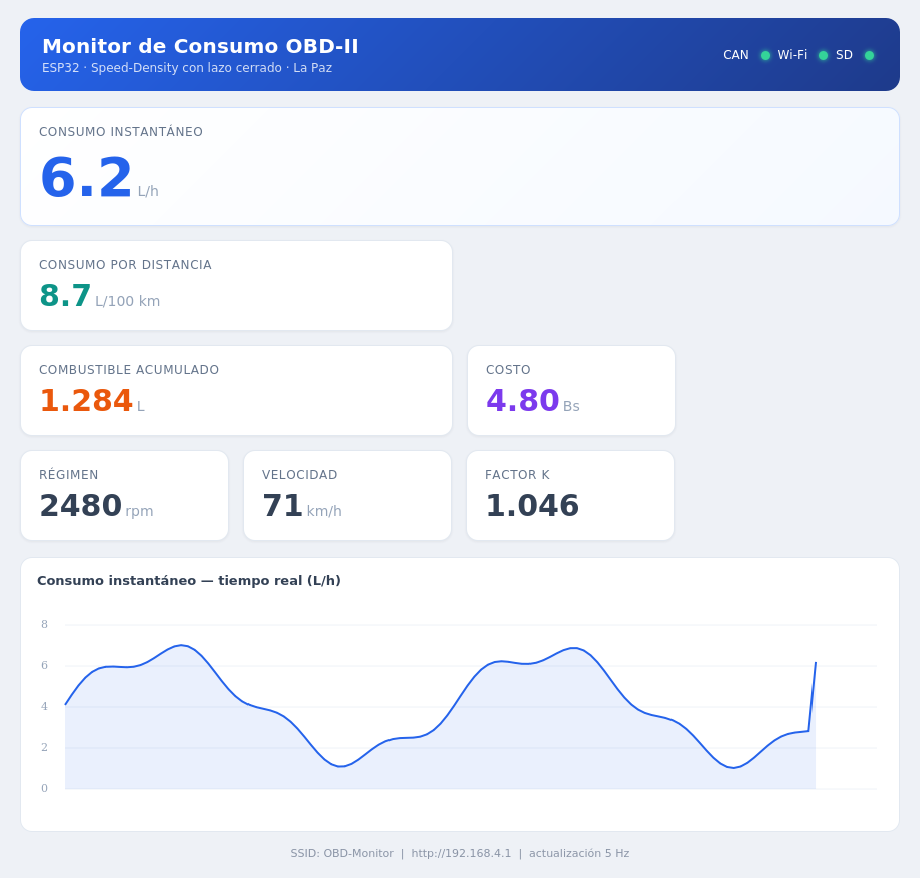
\includegraphics[width=0.75\textwidth]{Images/dashboard.png}
%
%	\vspace{4mm}
%	\small\raggedright
%	\textit{Nota.} Elaboración propia.
%	% Nota (APA): Elaboración propia.
%\end{figure}
%
%% ---------------------------------------------------------------------
%\subsection{Análisis de tiempos de respuesta y saturación de datos}
%\label{subsec:tiempos}
%
%La validez del sistema en tiempo real se sustenta en dos condiciones: que cada ciclo
%de adquisición quepa dentro de su periodo, y que ninguna cola ni canal se sature.
%
%\subsubsection{Presupuesto temporal del ciclo}
%
%La condición de tiempo real exige que el tiempo de ejecución del ciclo sea menor que
%el periodo asignado:
%
%\begin{equation}
%	T_\text{ciclo} + T_\text{cálculo} \;<\; T_\text{periodo},
%	\label{eq:presupuesto}
%\end{equation}
%
%donde $T_\text{ciclo}\approx 43\,\mathrm{ms}$ (Tabla~\ref{tab:tiempos-pid}),
%$T_\text{cálculo}<1\,\mathrm{ms}$ (operaciones en punto flotante e interpolación) y
%$T_\text{periodo}=250\,\mathrm{ms}$. El margen resultante es
%$250\,\mathrm{ms}-44\,\mathrm{ms}=206\,\mathrm{ms}$, equivalente a un
%\textbf{$82\pct$ de holgura}, suficiente para absorber latencias de ECU varias veces
%superiores a las típicas.
%
%\subsubsection{Saturación de colas y canal}
%
%La cola hacia la MicroSD no se satura mientras la tasa de producción sea menor que la
%de consumo:
%
%\begin{equation}
%	\lambda_\text{prod} = f_s = 4\ \text{muestras/s}
%	\;<\;
%	\mu_\text{consumo} = \frac{1}{\bar{T}_\text{escritura}},
%	\label{eq:cola}
%\end{equation}
%
%con $\bar{T}_\text{escritura}\approx 4{,}5\,\mathrm{ms/registro}$ (incluyendo el vaciado
%amortizado), lo que da $\mu\approx 220\,\mathrm{registros/s}\gg\lambda$. En consecuencia, la
%ocupación de la cola permanece cercana a~1 y el buffer de 32~no se llena.
%
%Para el canal WebSocket, el caudal de datos debe permanecer por debajo del ancho de
%banda del enlace Wi-Fi:
%
%\begin{equation}
%	S_\text{json}\cdot f_\text{web}\cdot N_\text{cli} \;<\; B_\text{Wi-Fi},
%	\label{eq:ws}
%\end{equation}
%
%con $S_\text{json}\approx 160\,\mathrm{bytes}$, $f_\text{web}=5\,\mathrm{Hz}$ y
%$N_\text{cli}$ clientes. Para $N_\text{cli}=4$ resulta
%$\approx 3{,}2\,\mathrm{kB/s}\approx 26\,\mathrm{kbps}$, muy por debajo del enlace; la limitación
%práctica es el número de estaciones que el punto de acceso del ESP32 admite con
%estabilidad (del orden de 4).
%
%\subsubsection{Instrumentación en firmware}
%
%Las métricas anteriores se miden directamente en ejecución
%(Figura~\ref{fig:cod-instr}): la latencia por PID con el temporizador de alta resolución,
%la ocupación de la cola con \texttt{uxQueueMessagesWaiting} y el margen de pila de
%cada tarea con \texttt{uxTaskGetStackHighWaterMark}. Estos valores se exponen por el
%puerto serie o el propio tablero, y constituyen la evidencia de validación.
%
%\begin{figure}[H]
%	\caption{Medicion de latencia, ocupacion de cola y margen de pila.}
%	\label{fig:cod-instr}
%	\begin{lstlisting}[language=C++]
%uint64_t t0 = esp_timer_get_time();     // microsegundos
%bool ok = obdRequest(pid) && obdRead(pid, buf, len, 60);
%uint64_t dt = esp_timer_get_time() - t0;// latencia del PID
%		
%uint32_t ocup = uxQueueMessagesWaiting(qLog);// ocupacion de la cola
%uint32_t pila = uxTaskGetStackHighWaterMark(NULL);// palabras libres min.
%uint8_t  cli  = WiFi.softAPgetStationNum();  // clientes Wi-Fi
%	\end{lstlisting}
%	
%
%\end{figure}
%
%La Tabla~\ref{tab:metricas} resume las métricas de validación con sus límites de
%diseño y el método de medición.
%
%\begin{table}[htbp]
%	\captionsetup{labelformat=simple, labelsep=newline, textfont=it, labelfont=bf, justification=raggedright, singlelinecheck=false}
%	\caption{Métricas de validación temporal y de saturación.}
%	\centering
%	\label{tab:metricas}
%	\begin{tabular}{@{}lll@{}}
%		\toprule
%		\rowcolor[rgb]{0.851, 0.851, 0.851}
%		\textbf{Métrica} & \textbf{Límite de diseño} & \textbf{Método de medición} \\
%		\midrule
%		Latencia por PID        & $<60\,\mathrm{ms}$ (timeout)        & \texttt{esp\_timer\_get\_time} \\
%		Tiempo de ciclo         & $<250\,\mathrm{ms}$ (periodo)       & acumulado por ciclo \\
%		Ocupación de cola       & $\ll 32$ ($\approx 1$)           & \texttt{uxQueueMessagesWaiting} \\
%		Margen de pila          & $>512\ \text{palabras}$           & \texttt{uxTaskGetStackHighWaterMark} \\
%		Caudal WebSocket        & $< B_\text{Wi-Fi}$               & Ec.~\eqref{eq:ws} \\
%		Clientes Wi-Fi          & $\le 4$                          & \texttt{softAPgetStationNum} \\
%		\bottomrule
%	\end{tabular}
%	
%	\vspace{2pt}
%	{\footnotesize\textit{Nota.} Elaboración propia.}
%\end{table}
%
%% ---------------------------------------------------------------------
%\subsection{Gestión de errores y robustez del sistema}
%\label{subsec:robustez}
%
%El firmware incorpora tres mecanismos de tolerancia a fallos, complementados por
%indicadores LED de estado en la PCB (alimentación, CAN activo, MicroSD y Wi-Fi).
%
%\textbf{Perro guardián (watchdog).} El temporizador watchdog de tareas (TWDT) del
%ESP32 vigila la tarea de adquisición. Si esta no se realimenta dentro del plazo
%configurado ---por ejemplo, porque el bus CAN quedó sin actividad y la tarea se
%bloqueó--- el TWDT reinicia el sistema, garantizando la recuperación autónoma
%(Figura~\ref{fig:cod-wdt}).
%
%\begin{figure}[H]
%	\caption{Configuracion del watchdog de tareas.}
%	\label{fig:cod-wdt}
%	\begin{lstlisting}[language=C++]
%esp_task_wdt_init(5, true);   // plazo 5 s; reinicia si vence
%esp_task_wdt_add(NULL);       // suscribe la tarea actual (adquisicion)
%// ... y dentro del lazo:  esp_task_wdt_reset();
%	\end{lstlisting}
%	
%
%\end{figure}
%
%\textbf{Recuperación de bus-off.} El controlador CAN entra en estado \emph{bus-off}
%cuando su contador de errores de transmisión (TEC) supera 255, desconectándose del
%bus \citep{bosch1991can}. El firmware detecta este estado y dispara la recuperación
%automática (Figura~\ref{fig:cod-busoff}); los contadores TEC/REC se monitorean para
%registrar la degradación antes de llegar a ese punto.
%
%\begin{figure}[H]
%	\caption{Deteccion y recuperacion de bus-off (TWAI).}
%	\label{fig:cod-busoff}
%	\begin{lstlisting}[language=C++]
%void canCheckHealth() {
%	twai_status_info_t st;
%	twai_get_status_info(&st);
%	if (st.state == TWAI_STATE_BUS_OFF) {
%		twai_initiate_recovery();        
%		// recupera tras 128x11 bits recesivos
%	} else if (st.state == TWAI_STATE_STOPPED) {
%		twai_start();   // reanuda tras recuperacion
%	}
%	// st.tx_error_counter 
%	// st.rx_error_counter > 96 -> registrar alerta
%}
%	\end{lstlisting}
%	
%
%\end{figure}
%
%\textbf{Estrategia de respaldo (fallback).} Si la ECU no responde durante varios
%ciclos consecutivos (superando un umbral configurable), la muestra se marca como
%inválida: el sistema conserva el último factor $K$ y la última curva $\eta_v$ válidos,
%mantiene en pantalla la última estimación fiable señalándola como no actualizada, y
%registra el evento. De este modo nunca se publican valores corruptos ni se pierde la
%calibración aprendida. La Tabla~\ref{tab:errores} sintetiza la matriz de errores.
%
%\begin{table}[H]
%	% Formato APA 7
%	\captionsetup{labelformat=simple, labelsep=newline, textfont=it, labelfont=bf, justification=raggedright, singlelinecheck=false}
%	\caption[Matriz de gestión de errores del sistema]{Matriz de gestión de errores del sistema embebido.}
%	\label{tab:errores}
%	\centering
%	
%	\vspace{2mm}
%	% Ampliamos los anchos de columna para evitar el amontonamiento de texto (Total ~14.5 cm)
%	\begin{tabular}{@{} p{3.5cm} p{3.5cm} p{4.5cm} p{3.0cm} @{}}
%		\toprule
%		\rowcolor[rgb]{0.851, 0.851, 0.851}
%		\textbf{Condición} & \textbf{Detección} & \textbf{Acción} & \textbf{Estado resultante} \\
%		\midrule
%		Sin respuesta de un PID & Timeout en \texttt{WAIT} ($>60\,\text{ms}$) & Descartar trama, reintentar en el siguiente ciclo & Operación normal \\
%		\addlinespace
%		Pérdida prolongada de CAN & $n$ ciclos sin respuesta & Marcar dato inválido, conservar $K$ y $\eta_v(N)$ & Modo degradado \\
%		\addlinespace
%		Bus-off del controlador & TWAI STATE BUS OFF & \texttt{twai\_initiate()} & Recuperación automática \\
%		\addlinespace
%		Tarea bloqueada & TWDT vence ($5\,\text{s}$) & Reinicio del sistema & Rearranque limpio \\
%		\addlinespace
%		Fallo de MicroSD & Error al abrir o escribir & Continuar sin registro, alertar por LED & Operación sin log \\
%		\bottomrule
%	\end{tabular}
%	
%	\vspace{4mm}
%	\small\raggedright
%	\textit{Nota.} Elaboración propia. La matriz detalla las contingencias consideradas en el diseño del firmware para asegurar la continuidad de la adquisición de datos de la ECU.
%\end{table}
%
%En conjunto, el diseño de software materializa el modelo en lazo cerrado sobre una
%arquitectura concurrente de dos núcleos, con subsistemas desacoplados, presupuesto
%temporal verificable y mecanismos de recuperación autónoma, satisfaciendo los
%requisitos de determinismo, robustez y confiabilidad del proyecto.
%
%\subsection{Gestión de energía y modo de reposo}
%\label{subsec:energia}
%
%El conector OBD-II mantiene el pin~16 con tensión de batería ($+12$~V) de forma
%permanente, incluso con el vehículo apagado. Por ello, un módulo conectado de forma
%fija queda energizado las 24~horas y, de no gestionarse su consumo, puede descargar
%gradualmente la batería. Esta subsección describe la estrategia para que el sistema
%entre en un modo de reposo de muy bajo consumo cuando el vehículo no está en uso y se
%reactive automáticamente al volver a encenderse.
%
%\subsubsection{Detección del vehículo inactivo}
%
%La detección se apoya en la actividad del bus CAN: mientras el contacto está activo, el
%bus presenta tráfico constante de las distintas ECU; al apagar el vehículo, el bus
%entra en reposo y deja de transmitir tramas tras unos minutos. El firmware aprovecha
%este comportamiento: si no se recibe ninguna trama válida durante un intervalo
%$T_\mathrm{idle}$ (por ejemplo, 90~s), concluye que el vehículo está apagado y procede
%a suspenderse. Como criterio complementario puede emplearse la tensión de la batería
%(con el motor en marcha el alternador la eleva a unos 14~V, frente a $\sim$12{,}4~V con
%el motor apagado), leída mediante un divisor resistivo.
%
%\subsubsection{Modos de bajo consumo del ESP32}
%
%El ESP32 ofrece varios modos de energía con distinto compromiso entre consumo y
%latencia de reactivación (Tabla~\ref{tab:modos-energia}). Para el reposo se selecciona
%el \emph{deep-sleep}, que reduce el consumo del microcontrolador a una fracción ínfima
%del de operación, a costa de reiniciar la ejecución al despertar ---lo cual es
%compatible con la persistencia en MicroSD ya implementada, que recupera el factor $K$
%y la curva $\eta_v$ tras cada arranque \citep{espressif_sleep}.
%
%\begin{table}[htbp]
%	\captionsetup{labelformat=simple, labelsep=newline, textfont=it, labelfont=bf, justification=raggedright, singlelinecheck=false}
%	
%	\caption{Modos de energía del ESP32 y su aplicación.}
%	\label{tab:modos-energia}
%	\centering
%	\begin{tabular}{@{}llll@{}}
%		\toprule
%		\rowcolor[rgb]{0.851, 0.851, 0.851}
%		\textbf{Modo} & \textbf{Consumo típico} & \textbf{Estado retenido} & \textbf{Reactivación} \\
%		\midrule
%		Activo (Wi-Fi activo)   & $\sim$150 mA          & completo              & inmediata \\
%		Activo (Wi-Fi inactivo) & $\sim$30 mA           & completo              & inmediata \\
%		Light-sleep             & $\sim$0{,}8 mA        & RAM y periféricos     & microsegundos \\
%		\textbf{Deep-sleep}     & $\sim$10 $\mu$A       & solo memoria RTC      & reinicio (\texttt{setup}) \\
%		\bottomrule
%	\end{tabular}
%\end{table}
%
%\subsubsection{Suspensión y reactivación}
%
%Antes de dormir, el firmware persiste la calibración, detiene el controlador TWAI y
%coloca el transceptor SN65HVD230 en modo \emph{standby} a través de su pin RS, lo que
%reduce su consumo a unos $0{,}2~\mu$A manteniendo la vigilancia del bus. Acto seguido
%configura las fuentes de despertar y entra en deep-sleep (Figura~\ref{fig:cod-sleep}).
%La fuente principal es la actividad del bus CAN: la línea RXD del transceptor
%se conecta a un GPIO con capacidad de despertar externo (\texttt{ext0}), de modo que la
%aparición de un bit dominante ---cuando el vehículo se enciende y el bus se reactiva---
%despierta al ESP32. Como respaldo se programa un despertar periódico por temporizador
%RTC que sondea brevemente el bus y vuelve a dormir si no detecta actividad. La
%Figura~\ref{fig:energia-fsm} resume la transición entre ambos modos.
%
%\begin{figure}[htbp]
%	\caption[Entrada en reposo profundo y despertar por actividad del bus]{Entrada en reposo
%		profundo y despertar por actividad del bus.}
%	\label{fig:cod-sleep}
%	\begin{lstlisting}[language=C++]
%#include "esp_sleep.h"
%#define WAKE_PIN  GPIO_NUM_4     // RXD del transceptor 
%#define T_IDLE_MS 90000          // 90 s sin tramas 
%
%uint32_t lastFrameMs = 0; // marca de la ultima trama recibida
%		
%void goToDeepSleep() {
%	saveK();              // persistir calibracion en MicroSD
%	twai_stop(); twai_driver_uninstall(); // liberar el controlador
%	digitalWrite(CAN_RS, HIGH); // SN65HVD230 -> standby (~0.2 uA)
%	// despertar cuando el bus vuelva a estar activo 
%	esp_sleep_enable_ext0_wakeup(WAKE_PIN, 0);
%	// respaldo: sondeo periodico cada 5 min
%	esp_sleep_enable_timer_wakeup(5ULL * 60 * 1000000);
%	esp_deep_sleep_start();      // ~10 uA hasta el despertar
%}
%
%// En el lazo principal, tras cada ciclo de adquisicion:
%//   if (millis() - lastFrameMs > T_IDLE_MS) goToDeepSleep();
%	\end{lstlisting}
%\end{figure}
%
%\begin{figure}[htbp]
%	
%	\caption{Transición entre el modo de operación y el modo de reposo de bajo consumo del
%		módulo, gobernada por la actividad del bus CAN.}
%	\label{fig:energia-fsm}
%	\centering
%	\vspace{2pt}
%	\resizebox{0.82\textwidth}{!}{%
%		\begin{tikzpicture}[
%			font=\normalsize,
%			base/.style={rectangle, draw, rounded corners, line width=0.8pt, align=center,
%				minimum height=1.5cm, minimum width=3.4cm},
%			act/.style={base, draw=green!60!black, fill=green!15},
%			slp/.style={base, draw=blue!70!black, fill=blue!12},
%			line/.style={-{Latex[length=2.8mm]}, line width=1.0pt, draw=black!75},
%			lbl/.style={font=\small, fill=white, inner sep=2.5pt, align=center}
%			]
%			\node[act] (act) {\textbf{ACTIVO}\\[2pt]\footnotesize adquisición + cálculo + web};
%			\node[slp, right=6.2cm of act] (slp) {\textbf{REPOSO}\\[2pt]\footnotesize deep-sleep ($\sim$10 $\mu$A)};
%			\draw[line] (act.north) .. controls +(0,1.2) and +(0,1.2) ..
%			node[lbl, above] {sin tráfico CAN $>$ $T_\mathrm{idle}$\\(detener TWAI, transceptor a standby)} (slp.north);
%			\draw[line] (slp.south) .. controls +(0,-1.2) and +(0,-1.2) ..
%			node[lbl, below] {actividad en el bus CAN (RXD)\\$\rightarrow$ despertar y reiniciar} (act.south);
%		\end{tikzpicture}%
%	}
%
%	% Nota (APA): Elaboración propia.
%\end{figure}
%
%\subsubsection{Presupuesto de energía y justificación del modo deep-sleep}
%
%Con el ESP32 en deep-sleep ($\sim$10~$\mu$A) y el transceptor SN65HVD230 en standby
%($\sim$0{,}2~$\mu$A), el consumo en reposo queda dominado por la corriente de
%	reposo (IQ) del convertidor TPS54331, del orden de $\sim$2{,}5~mA. El consumo
%acumulado durante el período máximo de inactividad del vehículo ---estimado en
%\textbf{3 días}--- se calcula como:
%
%\begin{equation}
%	Q_\mathrm{reposo} = I_\mathrm{reposo} \times t_\mathrm{max}
%	= 2{,}5\,\mathrm{mA} \times 72\,\mathrm{h} = 180\,\mathrm{mAh}.
%	\label{eq:q-reposo}
%\end{equation}
%
%Referida a la capacidad nominal de una batería de automóvil típica (45~Ah), esta
%energía representa:
%
%\begin{equation}
%	\frac{Q_\mathrm{reposo}}{C_\mathrm{bat}} =
%	\frac{180\,\mathrm{mAh}}{45{,}000\,\mathrm{mAh}} \approx 0{,}4\,\%.
%	\label{eq:porcentaje-bat}
%\end{equation}
%
%Un $0{,}4\,\%$ de la capacidad de la batería es prácticamente despreciable,
%especialmente considerando que el propio vehículo ya presenta corrientes parásitas en
%reposo de 20--50~mA (reloj, alarma, ECUs en standby), frente a los cuales los
%2{,}5~mA del módulo representan una fracción menor. Además, al volver a encenderse, el
%alternador recupera esos 180~mAh en cuestión de minutos de marcha. En consecuencia,
%el modo deep-sleep del ESP32 es suficiente para el caso de uso del presente
%	proyecto, sin necesidad de modificación de hardware. La desconexión completa del rail
%de 3{,}3~V (power-gating del convertidor buck) se plantea como recomendación para
%versiones futuras del módulo en escenarios de inactividad prolongada.
%
%La Tabla~\ref{tab:energia} consolida el presupuesto de energía comparando los tres
%escenarios posibles.
%
%\begin{table}[htbp]
%	\captionsetup{labelformat=simple, labelsep=newline, textfont=it, labelfont=bf, justification=raggedright, singlelinecheck=false}
%	
%	\caption{Presupuesto de energía en operación y en reposo.}
%	\label{tab:energia}
%	\centering
%	\resizebox{\textwidth}{!}{%
%		\begin{tabular}{@{}p{3.8cm}ccccl@{}}
%			\toprule
%			\rowcolor[rgb]{0.851, 0.851, 0.851}
%			\textbf{Estado} & \textbf{ESP32} & \textbf{Transc.}
%			& \textbf{TPS54331 IQ} & \textbf{Total@bat.} & \textbf{3 días acum.} \\
%			\midrule
%			Operación (adq.+Wi-Fi)
%			& $\sim$150 mA & $\sim$5 mA & $\sim$0{,}12 mA & $\sim$50 mA$^{\dagger}$ & --- \\[4pt]
%			\textbf{Reposo (deep-sleep)}
%			& 10 $\mu$A & 40 $\mu$A & 116 $\mu$A$^{*}$
%			& $\sim$\textbf{0{,}14 mA} & \textbf{10 mAh (0,02\,\%)} \\[4pt]
%			Reposo + power-gating
%			& apagado & apagado & apagado & $<$20 $\mu$A & $<$1{,}5 mAh \\
%			\bottomrule
%		\end{tabular}}
%	
%	\vspace{4pt}
%	{\footnotesize
%		$^{*}$ IQ típico del TPS54331DR según hoja de datos de Texas Instruments;
%		valor a verificar por medición directa del módulo ensamblado.\\
%		$^{\dagger}$ Corriente desde batería (12~V): $P_\mathrm{out}/(V_\mathrm{bat}\times\eta)
%		= (3{,}3\,\mathrm{V}\times155\,\mathrm{mA})/(12\,\mathrm{V}\times0{,}85)\approx50\,\mathrm{mA}$.
%		El porcentaje de capacidad se calcula respecto a una batería de 45~Ah.}
%\end{table}
%En conjunto, el diseño de software materializa el modelo en lazo cerrado sobre una
%arquitectura concurrente de dos núcleos, con subsistemas desacoplados, presupuesto
%temporal verificable, gestión de energía en reposo y mecanismos de recuperación
%autónoma, satisfaciendo los requisitos de determinismo, robustez, eficiencia energética
%y confiabilidad del proyecto.
	% !TEX root = ../main.tex
% ============================================================================
% CAPÍTULO 4 — IMPLEMENTACIÓN Y PRUEBAS
% ----------------------------------------------------------------------------
% NOTAS DE USO (borrar este bloque antes de la entrega final):
%   1. Este archivo asume \usepackage{booktabs} y \usepackage{graphicx} en el
%      preámbulo del documento principal. Si tu main.tex no los tiene, agrégalos.
%   2. Todo texto entre corchetes [COMPLETAR: ...] debe reemplazarse con tus
%      datos reales una vez realizadas las pruebas. Las tablas de resultados
%      contienen valores de EJEMPLO (marcados como tal) solo para mostrar el
%      formato; no son datos reales y no deben citarse como si lo fueran.
%   3. Los bloques de figura son marcadores de posición (cajas grises). Cuando
%      tengas la fotografía o gráfica, reemplaza el contenido del \fbox por
%      \includegraphics[width=0.8\textwidth]{ruta/imagen.png}.
%   4. Numeración: al usar \chapter, las tablas y figuras se numerarán como
%      4.1, 4.2, etc. automáticamente (asumiendo que este es el capítulo 4).
%   5. Las citas usan \citep{} (estilo natbib/apalike), coherente con el resto
%      de tu tesis. Las entradas .bib están en referencias_cap4.bib adjunto.
%   6. Redacción en tono impersonal/pasivo y en tiempo presente o pretérito,
%      sin primera persona ni futuro, siguiendo los criterios de estilo que
%      ya identificaste para el tribunal (separador decimal con coma, sin
%      "etc.", uso reducido de "el cual/la cual").
% ============================================================================

\chapter{IMPLEMENTACIÓN Y PRUEBAS}

Este capítulo describe el proceso de implementación física del sistema de monitoreo de consumo de combustible, desde el prototipado en protoboard hasta pruebas con la placa de circuito impreso (PCB) definitiva, y expone la metodología experimental empleada para validar su desempeño en condiciones reales de operación. La validación se realiza sobre dos vehículos de características distintas y se contrasta contra un adaptador ELM327 combinado con una aplicación comercial de cálculo de consumo. Esta comparación permite evaluar tanto la exactitud del método de estimación como la fiabilidad del sistema desarrollado frente a una alternativa disponible en el mercado.

\section{Montaje del sistema}

El montaje del sistema se organiza en dos etapas complementarias. En la primera, se ensambla un prototipo funcional sobre protoboard que permite verificar la viabilidad eléctrica y de firmware de la arquitectura propuesta antes de comprometer recursos en la fabricación de la PCB. En la segunda etapa, una vez validado el prototipo, se envía el diseño definitivo a fabricación bajo el proceso de JLCPCB. Este orden de trabajo reduce el riesgo de errores de diseño irreversibles en la placa final y permite depurar el firmware con mayor libertad de modificación del cableado.

\subsection{Prototipado en protoboard}

El prototipo se construye alrededor de la placa de desarrollo ESP32-S3-DevKitC-1 (módulo ESP32-S3-WROOM-1, variante N16R8), que integra el controlador CAN nativo TWAI, evitando así la necesidad del controlador externo MCP2515 empleado en la arquitectura inicial del proyecto. La Tabla~\ref{tab:componentes_protoboard} resume los componentes utilizados en esta etapa.



Siguiendo el proceso de armado:

\begin{itemize}
	\item Colocar primeramente el ESP32-S3 en una ubicación fácil de programar y de alimentar por su puerto de comunicación.
	\item Colocar estratégicamente el SN65HDV230 junto con el OLED, ya que estos componentes comparten una alimentación de 3.3~V.
	\item Después para no arruinar un micro SD se usa un adaptador SD, el cual soldaremos para una mejor conexión al protoboard.
	\item Y como ultimo se conecta una configuración de 4 leds para ayudar la visualización de los periféricos.
	
\end{itemize}

\begin{table}[H]
	\centering
	\captionsetup{labelformat=simple, labelsep=newline, textfont=it, labelfont=bf, justification=raggedright, singlelinecheck=false}
	\caption{Componentes empleados en el prototipo sobre protoboard}
	\label{tab:componentes_protoboard}
	\begin{tabularx}{\textwidth}{>{\raggedright\arraybackslash}p{4.5cm} X >{\centering\arraybackslash}p{2cm}}
		\toprule
		\rowcolor[rgb]{0.851, 0.851, 0.851}
		Componente & Función en el prototipo & Cantidad \\
		\midrule
		ESP32-S3-DevKitC-1 (N16R8) & Unidad de procesamiento principal, TWAI nativo & 1 \\
		Módulo transceptor SN65HVD230 & Adaptación de niveles para el bus CAN & 1 \\
		Módulo lector de tarjeta MicroSD (SPI) & Registro local de datos & 1 \\
		Pantalla OLED SSD1306 (I2C) & Visualización de parámetros en tiempo real & 1 \\
		Módulo regulador step-down 12\,V a 5\,V & Alimentación desde el conector OBD-II & 1 \\
		Conector OBD-II tipo A con cable & Interfaz física con el vehículo & 1 \\
		Protoboard, cables jumper macho-macho y macho-hembra & Interconexión temporal de los módulos & Variable \\
		\bottomrule
	\end{tabularx}
	\vspace{2mm}
	\\
	\begin{minipage}{\linewidth}
		\small 
		
		\textit{Nota.} Relación de elementos de hardware integrados para el montaje preliminar y validación de comunicaciones del sistema.
	\end{minipage}
\end{table}

La Figura~\ref{fig:prototipo} muestra la disposición física del prototipo, referenciada a lo largo de esta sección.

\begin{figure}[H]
	\centering
	\caption{Componentes del prototipo y elementos principales del sistema.}
	\label{fig:prototipo}
	
	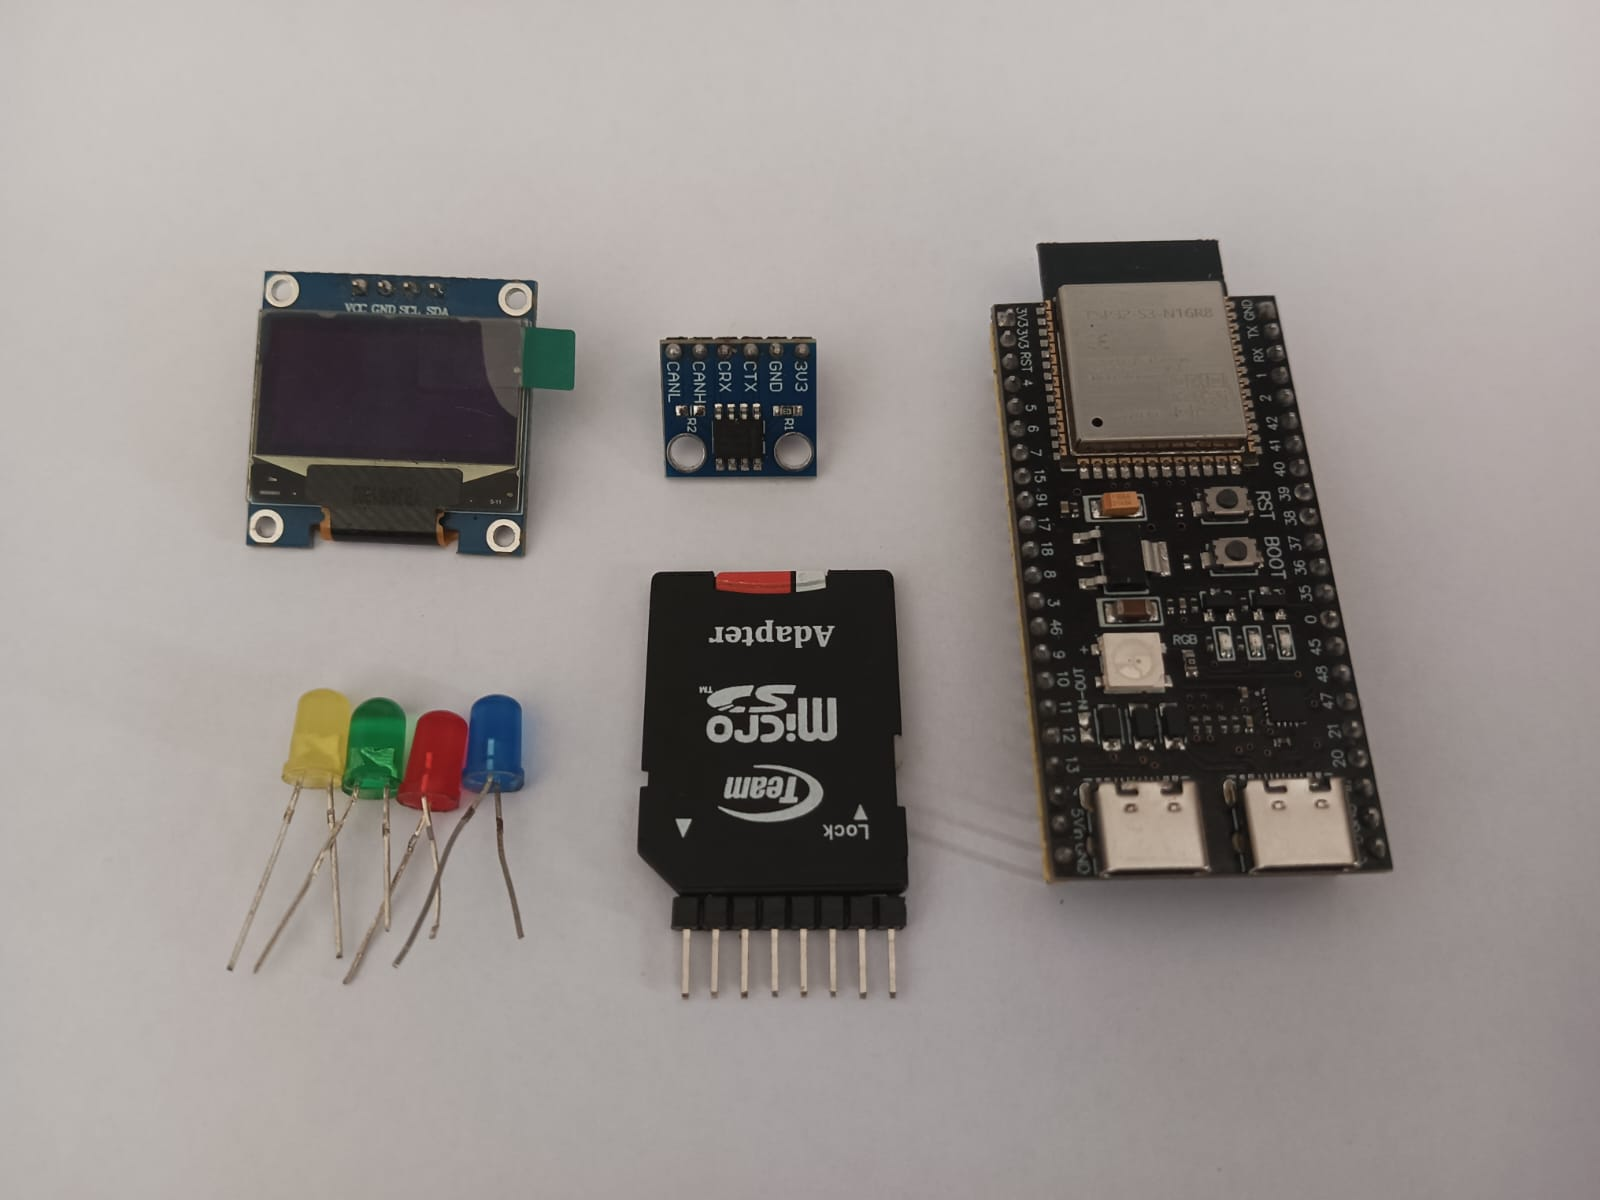
\includegraphics[width=0.8\textwidth]{Images/compo.jpeg}
	\\
	\vspace{2pt}
	{\footnotesize\textit{Nota.} Esquema detallado del patillaje y la comunicación serie entre el microcontrolador principal y los periféricos del sistema. Elaboración propia.}
	
\end{figure}



\subsection{Integración del módulo ESP32-S3 y periféricos en protoboard}

La asignación de pines para el prototipo se resume en la Tabla~\ref{tab:asignacion_pines}. Tal como se presentó en el esquemático de conexión dentro de la sección de diseño de software, esta misma distribución se mantiene para el prototipado físico (Tabla~\ref{tab:mapa_pines}).

\begin{table}[H]
	\centering
	\captionsetup{labelformat=simple, labelsep=newline, textfont=it, labelfont=bf, justification=raggedright, singlelinecheck=false}
	\caption{Asignación de pines GPIO del ESP32-S3 en el prototipo}
	\label{tab:asignacion_pines}
	\begin{tabularx}{\textwidth}{>{\raggedright\arraybackslash}p{4cm} >{\raggedright\arraybackslash}p{4cm} X}
		\toprule
		\rowcolor[rgb]{0.851, 0.851, 0.851}
		Periférico & Pines GPIO & Observaciones \\
		\midrule
		Bus CAN (TWAI) & TX: GPIO4, RX: GPIO5 & Modo listen-only durante pruebas comparativas \\
		Bus I2C (pantalla OLED) & SDA: GPIO8, SCL: GPIO9 & Dirección I2C del controlador SSD1306 \\
		Bus SPI (MicroSD) & MOSI/MISO/SCK/CS: GPIO11-GPIO14 & Sistema de archivos FAT32 \\
		Control de load switches (TPS22918DBVR) & GPIO6,GPIO10 & Habilitación activa en alto (HIGH) \\
		UART de programación & TXD0/RXD0 & Uso exclusivo durante flasheo y depuración \\
		\bottomrule
	\end{tabularx}
	\vspace{2mm}
	\\
	\begin{minipage}{\linewidth}
		\small
		\textit{Nota.} Mapeo de la distribución física de señales digitales y buses de comunicación configurados en el microcontrolador principal.
	\end{minipage}
\end{table}



\begin{figure}[H]
	\centering
	\caption{Diagrama de interconexión de periféricos en el prototipo}
	\label{fig:diagrama_perifericos}
	\begin{tikzpicture}
		
		% Imagen original
		\node[inner sep=0pt] (foto) {
			
\includegraphics[width=0.85\textwidth]{images/prototipo.jpg}
		};
		
		% ------------------------------------------------
		% ESP32
		% ------------------------------------------------
		\node[
		draw=red,
		very thick,
		rounded corners=3pt,
		fill=white,
		align=center,
		font=\bfseries,
		minimum width=2.5cm,
		minimum height=0.8cm
		] (esp32) at ([xshift=-1.0cm,yshift=-0.8cm]foto.north east)
		{ESP32};
		
		\draw[
		->,
		red,
		very thick
		]
		(esp32.west)
		-- ([xshift=-6.3cm,yshift=-4.3cm]foto.north east);
		
		% ------------------------------------------------
		% LEDs
		% ------------------------------------------------
		\node[
		draw=green!60!black,
		very thick,
		rounded corners=3pt,
		fill=white,
		align=center,
		font=\bfseries,
		minimum width=2.5cm,
		minimum height=0.8cm
		] (leds) at ([xshift=0.8cm,yshift=-0.8cm]foto.north west)
		{LEDs};
		
		\draw[
		->,
		green!60!black,
		very thick
		]
		(leds.east)
		-- ([xshift=6.8cm,yshift=-0.8cm]foto.north west);
		
		% ------------------------------------------------
		% OLED
		% ------------------------------------------------
		\node[
		draw=blue,
		very thick,
		rounded corners=3pt,
		fill=white,
		align=center,
		font=\bfseries,
		minimum width=2.5cm,
		minimum height=0.8cm
		] (oled) at ([xshift=0.8cm,yshift=-3.8cm]foto.north west)
		{OLED};
		
		\draw[
		->,
		blue,
		very thick
		]
		(oled.east)
		-- ([xshift=2.8cm,yshift=-6.3cm]foto.north west);
		
		% ------------------------------------------------
		% Tarjeta SD
		% ------------------------------------------------
		\node[
		draw=orange!80!black,
		very thick,
		rounded corners=3pt,
		fill=white,
		align=center,
		font=\bfseries,
		minimum width=2.8cm,
		minimum height=0.8cm
		] (sd) at ([xshift=-1.0cm,yshift=0.8cm]foto.south east)
		{Tarjeta SD};
		
		\draw[
		->,
		orange!80!black,
		very thick
		]
		(sd.west)
		-- ([xshift=-3.0cm,yshift=3.5cm]foto.south east);
		
		% ------------------------------------------------
		% SN65HVD230
		% ------------------------------------------------
		\node[
		draw=violet,
		very thick,
		rounded corners=3pt,
		fill=white,
		align=center,
		font=\bfseries,
		minimum width=3.5cm,
		minimum height=0.8cm
		] (can) at ([xshift=0cm,yshift=0.8cm]foto.south)
		{SN65HVD230};
		
		\draw[
		->,
		violet,
		very thick
		]
		(can.north)
		-- ([xshift=0cm,yshift=2.3cm]foto.south);
		
	\end{tikzpicture}
	\vspace{2pt}
	\\
	{\footnotesize\textit{Nota.} Vista general del prototipo con etiquetas identificativas para cada módulo interactivo. Elaboración propia.}
	
\end{figure}

La integración se verifica de manera incremental: primero se confirma la comunicación I2C con la pantalla OLED mediante un barrido de direcciones (\textit{I2C scanner}), luego se valida la escritura y lectura en la tarjeta MicroSD, y finalmente se habilita el controlador TWAI para la recepción de tramas CAN, como se detalla en la Figura~\ref{fig:diagrama_perifericos}.

\subsection{Placa preliminar en EasyEDA}
\label{sec:placa_preliminar}

Una vez concluidas las pruebas de campo sobre el prototipo en protoboard, se diseñó en EasyEDA una placa preliminar que replica el mismo circuito funcional ya validado (mismo módulo ESP32-S3, mismo transceptor CAN, misma pantalla OLED y microSD), con el único fin de contar con una versión más robusta y cómoda de manejar que las conexiones sueltas de una protoboard, previa a la placa final documentada en el Capítulo~3 (diseñada en Altium Designer). A diferencia de esa placa final, la preliminar resuelve la alimentación con un regulador lineal simple en vez de la conversión conmutada de dos rieles, suficiente para las pruebas de campo dado que no corre con la misma restricción de autonomía en reposo; el esquemático completo, la simulación 3D y las fotografías de la placa fabricada se presentan en el Capítulo~3 (Sección~\ref{sec:pcb_preliminar_diseno}). La fabricación de esta placa preliminar se encargó a Robokit (La Paz) por 150\,Bs (Tabla~\ref{tab:costo_pcb_preliminar}, Capítulo~5), y el ensamblaje de los componentes se realizó manualmente. Al tratarse del mismo circuito ya probado, esta placa no requirió una nueva ronda de pruebas de campo: su función es exclusivamente de robustez física y comodidad de manejo, no de validación técnica adicional sobre lo ya reportado en este capítulo.

\subsection{Conexión al bus CAN del vehículo}

La conexión física al vehículo se realiza a través del conector estandarizado de 16 pines J1962, cuya asignación depende del protocolo de comunicación soportado; desde 2008 la práctica totalidad de los vehículos livianos emplea el protocolo ISO 15765 sobre bus CAN \citep{iso15765}. La Tabla~\ref{tab:pinout_obd} resume los pines relevantes para este proyecto.

\begin{table}[H]
	\centering
	\captionsetup{labelformat=simple, labelsep=newline, textfont=it, labelfont=bf, justification=raggedright, singlelinecheck=false}
	\caption{Pines relevantes del conector OBD-II (J1962) utilizados en el proyecto}
	\label{tab:pinout_obd}
	\begin{tabularx}{\textwidth}{>{\centering\arraybackslash}p{1.5cm} >{\raggedright\arraybackslash}p{4cm} X}
		\toprule
		\rowcolor[rgb]{0.851, 0.851, 0.851}
		Pin & Señal & Uso en el sistema \\
		\midrule
		6 & CAN High (CAN\_H) & Línea diferencial positiva del bus CAN \\
		14 & CAN Low (CAN\_L) & Línea diferencial negativa del bus CAN \\
		16 & Alimentación +12\,V & Entrada al regulador TPS54302DDCR \\
		4 y 5 & Tierra (chasis y señal) & Referencia común del sistema \\
		\bottomrule
	\end{tabularx}
	\vspace{2mm}
	\\
	\begin{minipage}{\linewidth}
		\small
		\textit{Nota.} Identificación de las líneas físicas de alimentación y comunicación del estándar J1962 requeridas para la interfaz con el vehículo.
	\end{minipage}
\end{table}

Con el fin de evitar que el sistema propio introduzca tramas de solicitud adicionales que puedan interferir con el adaptador comercial, el controlador TWAI del ESP32-S3 se configura en modo de solo escucha (\textit{listen-only}), de manera que únicamente recibe y decodifica las tramas sin transmitir reconocimientos ni solicitudes propias. En la Figura \ref{fig:conexion_can}

\begin{figure}[htbp]
	\centering
	\caption{Conexión del sistema propuesto mediante OBD-II}
	\label{fig:conexion_can}
	\begin{tikzpicture}
		
		% Imagen original
		\node[inner sep=0pt] (foto) {
			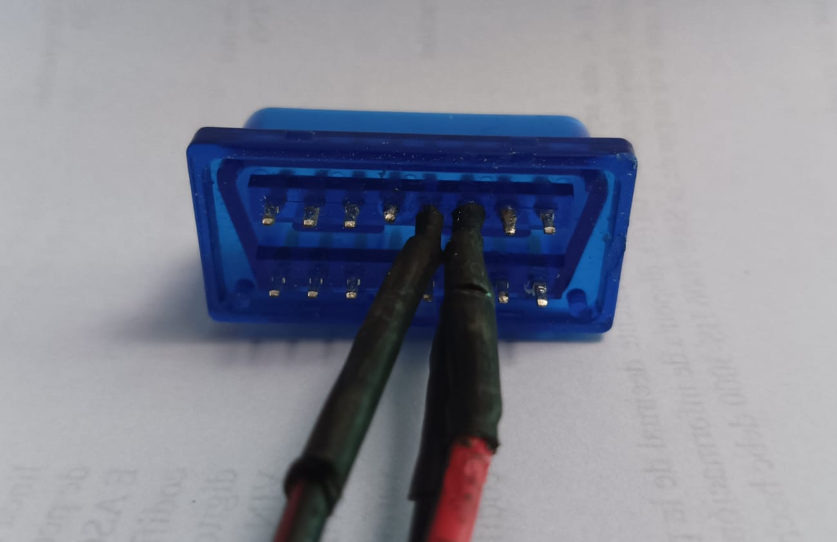
\includegraphics[width=0.7\textwidth]{Images/OBD.png}
		};
		
		% ------------------------------------------------
		% GND (Pin 5) - Arriba Izquierda
		% ------------------------------------------------
		\node[
		draw=blue,
		very thick,
		rounded corners=3pt,
		fill=white,
		align=center,
		font=\bfseries,
		minimum width=2.5cm,
		minimum height=0.8cm
		] (gnd) at ([xshift=-0.5cm,yshift=-0.8cm]foto.north west)
		{GND (Pin 5)};
		
		\draw[
		->,
		blue,
		very thick
		]
		(gnd.east)
		-- ([xshift=5.5cm,yshift=-2.5cm]foto.north west);
		
		% ------------------------------------------------
		% CAN_H (Pin 6) - Arriba Derecha
		% ------------------------------------------------
		\node[
		draw=red,
		very thick,
		rounded corners=3pt,
		fill=white,
		align=center,
		font=\bfseries,
		minimum width=2.5cm,
		minimum height=0.8cm
		] (canh) at ([xshift=0.5cm,yshift=-0.8cm]foto.north east)
		{CAN\_H (Pin 6)};
		
		\draw[
		->,
		red,
		very thick
		]
		(canh.west)
		-- ([xshift=-4.8cm,yshift=-2.9cm]foto.north east);
		
		% ------------------------------------------------
		% CAN_L (Pin 14) - Abajo Derecha
		% ------------------------------------------------
		\node[
		draw=green!60!black,
		very thick,
		rounded corners=3pt,
		fill=white,
		align=center,
		font=\bfseries,
		minimum width=2.5cm,
		minimum height=0.8cm
		] (canl) at ([xshift=0.5cm,yshift=-3.5cm]foto.north east)
		{CAN\_L (Pin 14)};
		
		\draw[
		->,
		green!60!black,
		very thick
		]
		(canl.west)
		-- ([xshift=-4.8cm,yshift=-3.8cm]foto.north east);
		
	\end{tikzpicture}
	\\
	\vspace{2pt}
	{\footnotesize\textit{Nota.} Fotografía de la interfaz OBD-II del vehículo mostrando la derivación del bus CAN. Elaboración propia.}

\end{figure}


\subsection{Instalación física en el vehículo de pruebas}

Buscamos para hacer las pruebas en campo , primero ubicar el puerto OBD2 del vehiculo el cual se ecuentra casi siempre abajo del volante arriba de los pedales, algunos a primera vista otros hay que desarmar unas piezas para llegar a su ubicacion.

En la Figura \ref{fig:instalacion_vehiculo} mostramos la ubicacion de uno de los vehiculos a ponerlo a prueba el cual se desarmo una parte para acceder este se encontro junto alos fusibles de los tableros.

\begin{figure}[H]
	\centering
	\caption{Identificación física del OBD2 en el vehículo antes de las pruebas}
	\label{fig:instalacion_vehiculo}
	\begin{tikzpicture}
		
		% Imagen original
		\node[inner sep=0pt] (foto) {
			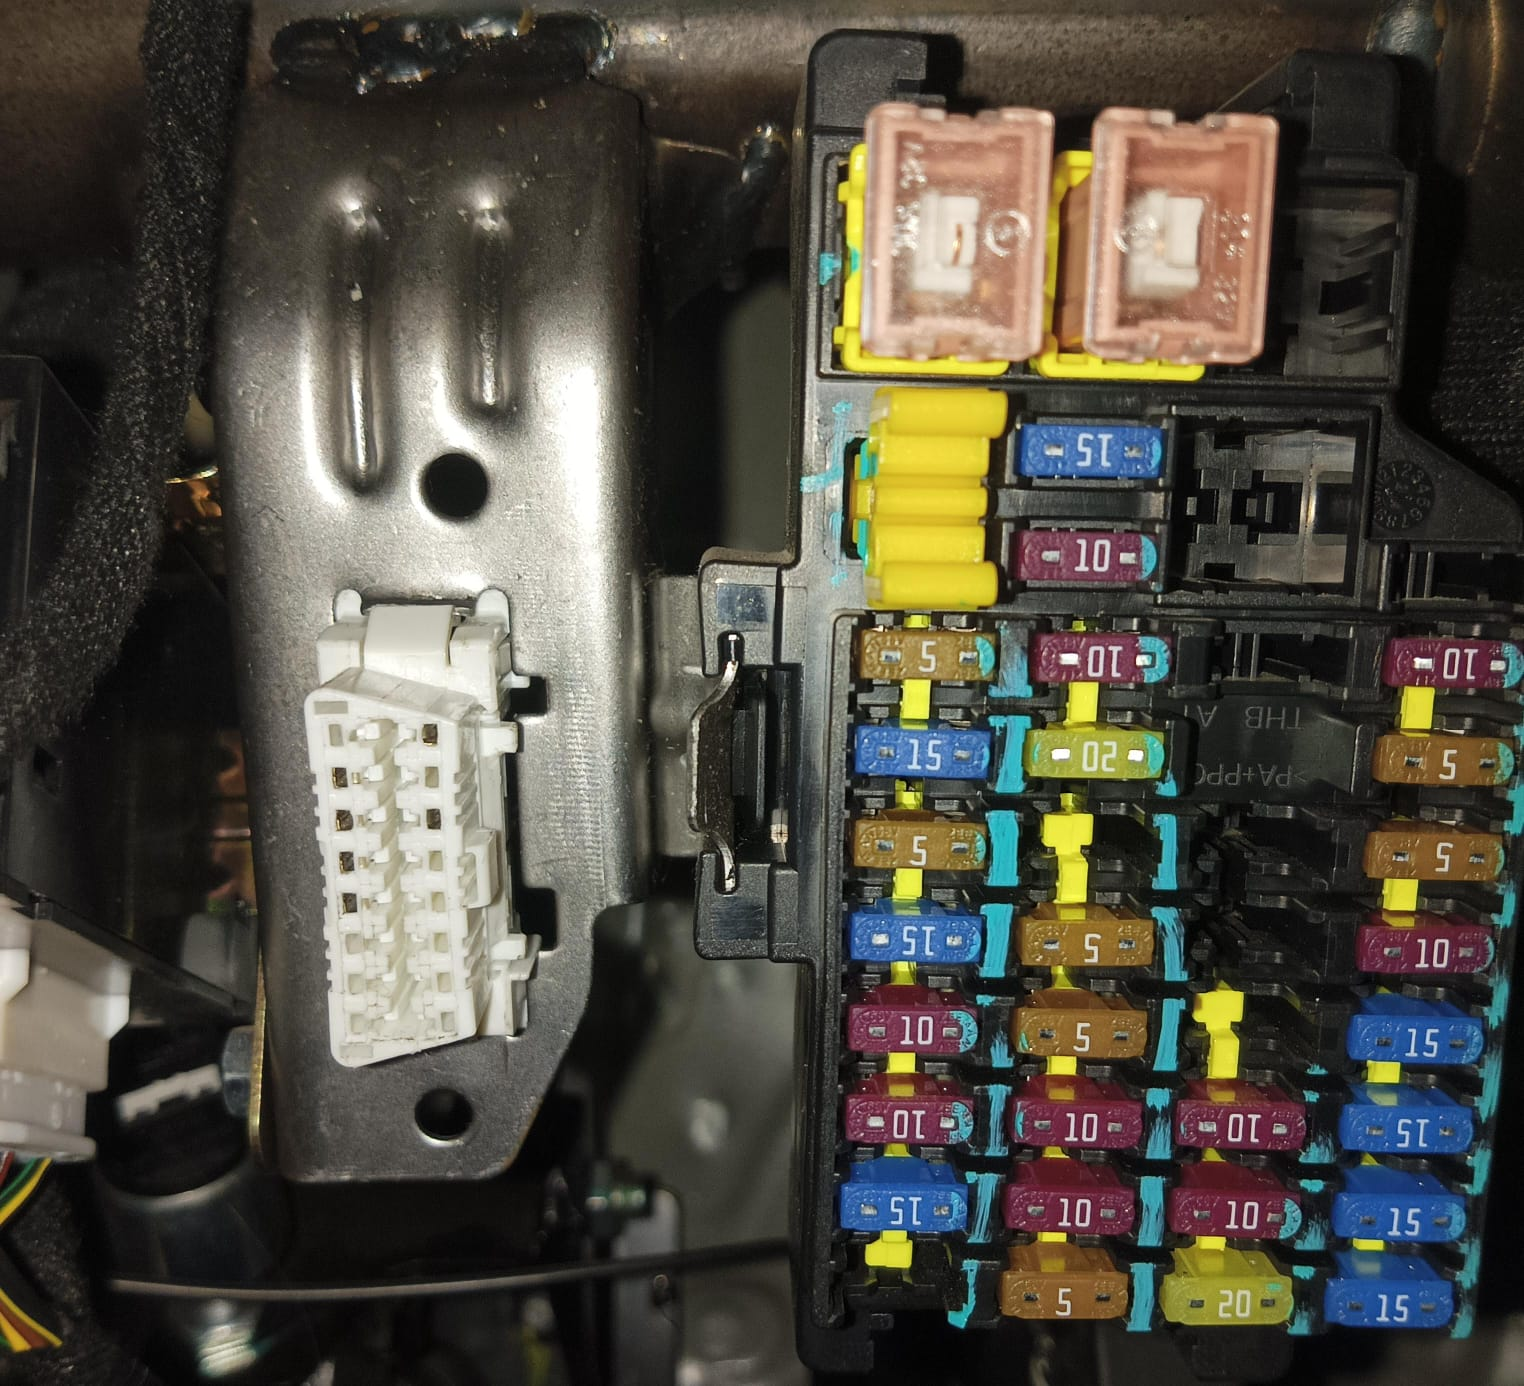
\includegraphics[width=0.55\textwidth]{Images/OBD_CON.jpeg}
		};
		
		% ------------------------------------------------
		% Conector OBD2 (Hembra) - Izquierda
		% ------------------------------------------------
		\node[
		draw=blue,
		very thick,
		rounded corners=3pt,
		fill=white,
		align=center,
		font=\bfseries,
		minimum width=3.8cm,
		minimum height=0.8cm
		] (obd) at ([xshift=-1.0cm,yshift=-2.0cm]foto.north west)
		{Conector OBD2\\(Hembra)};
		
		\draw[
		->,
		blue,
		very thick
		]
		(obd.east)
		-- ([xshift=2.0cm,yshift=-3.8cm]foto.north west);
		
		% ------------------------------------------------
		% 2do Tablero de Fusibles - Derecha
		% ------------------------------------------------
		\node[
		draw=red,
		very thick,
		rounded corners=3pt,
		fill=white,
		align=center,
		font=\bfseries,
		minimum width=3.8cm,
		minimum height=0.8cm
		] (fusibles) at ([xshift=1.0cm,yshift=-2.0cm]foto.north east)
		{2do Tablero de\\Fusibles};
		
		\draw[
		->,
		red,
		very thick
		]
		(fusibles.west)
		-- ([xshift=-2.8cm,yshift=-3.0cm]foto.north east);
		
	\end{tikzpicture}
	
	\vspace{2pt}
	{\footnotesize\textit{Nota.} Vista general del dispositivo dentro del habitáculo del vehículo. Elaboración propia.}
\end{figure}

Con el objetivo de que el dispositivo se instale de manera que no obstruye los controles del conductor y permite el acceso visual a la pantalla OLED durante la conducción.

\section{Configuración del entorno de pruebas}

\subsection{Vehículos utilizados para la validación}

La validación experimental se realiza sobre dos vehículos con arquitecturas de motor distintas. Esto permite evaluar la capacidad de generalización del método Speed-Density ante diferentes configuraciones de inyección y gestión electrónica. La Tabla~\ref{tab:vehiculos} resume sus características principales.

\begin{table}[H]
	\centering
	\captionsetup{labelformat=simple, labelsep=newline, textfont=it, labelfont=bf, justification=raggedright, singlelinecheck=false}
	\caption{Vehículos utilizados en la fase de validación experimental}
	\label{tab:vehiculos}
	\begin{tabularx}{\textwidth}{>{\raggedright\arraybackslash}p{4cm} X X}
		\toprule
		\rowcolor[rgb]{0.851, 0.851, 0.851}
		Característica & Changan Honor & Nissan Vanette \\
		\midrule
		Año de fabricación & 2023 & 2018 \\
		Cilindrada & 1298 mL & 1626 mL \\
		Capacidad de tanque & 40 L & 60 L \\
		Tipo de inyección & Electrónica & Electrónica \\
		Combustible & Gasolina & Gasolina \\
		Protocolo OBD-II & ISO 15765-4 & ISO 15765-4 \\
		Kilometraje aproximado & 5210 & 98765 \\
		Uso habitual & Particular y/o comercial & Cargamento \\
		\bottomrule
	\end{tabularx}
	\vspace{2mm}
	\\
	\begin{minipage}{\linewidth}
		\small
		\textit{Nota.} Ficha técnica comparativa de las unidades vehiculares empleadas para las pruebas de lectura de datos en el bus CAN y la recolección en campo.
	\end{minipage}
\end{table}

La diferencia de antigüedad entre ambos vehículos (2023 frente a 2018) permite además evaluar el comportamiento del sistema frente a posibles variaciones en la calibración de fábrica de los sensores MAP y en el desgaste mecánico propio de un motor con mayor kilometraje.

\begin{figure}[H]
	\centering
	\caption{Vehículos de prueba utilizados en la validación experimental}
	\label{fig:vehiculos_prueba}
	\begin{subfigure}[t]{0.48\textwidth}
		\centering
		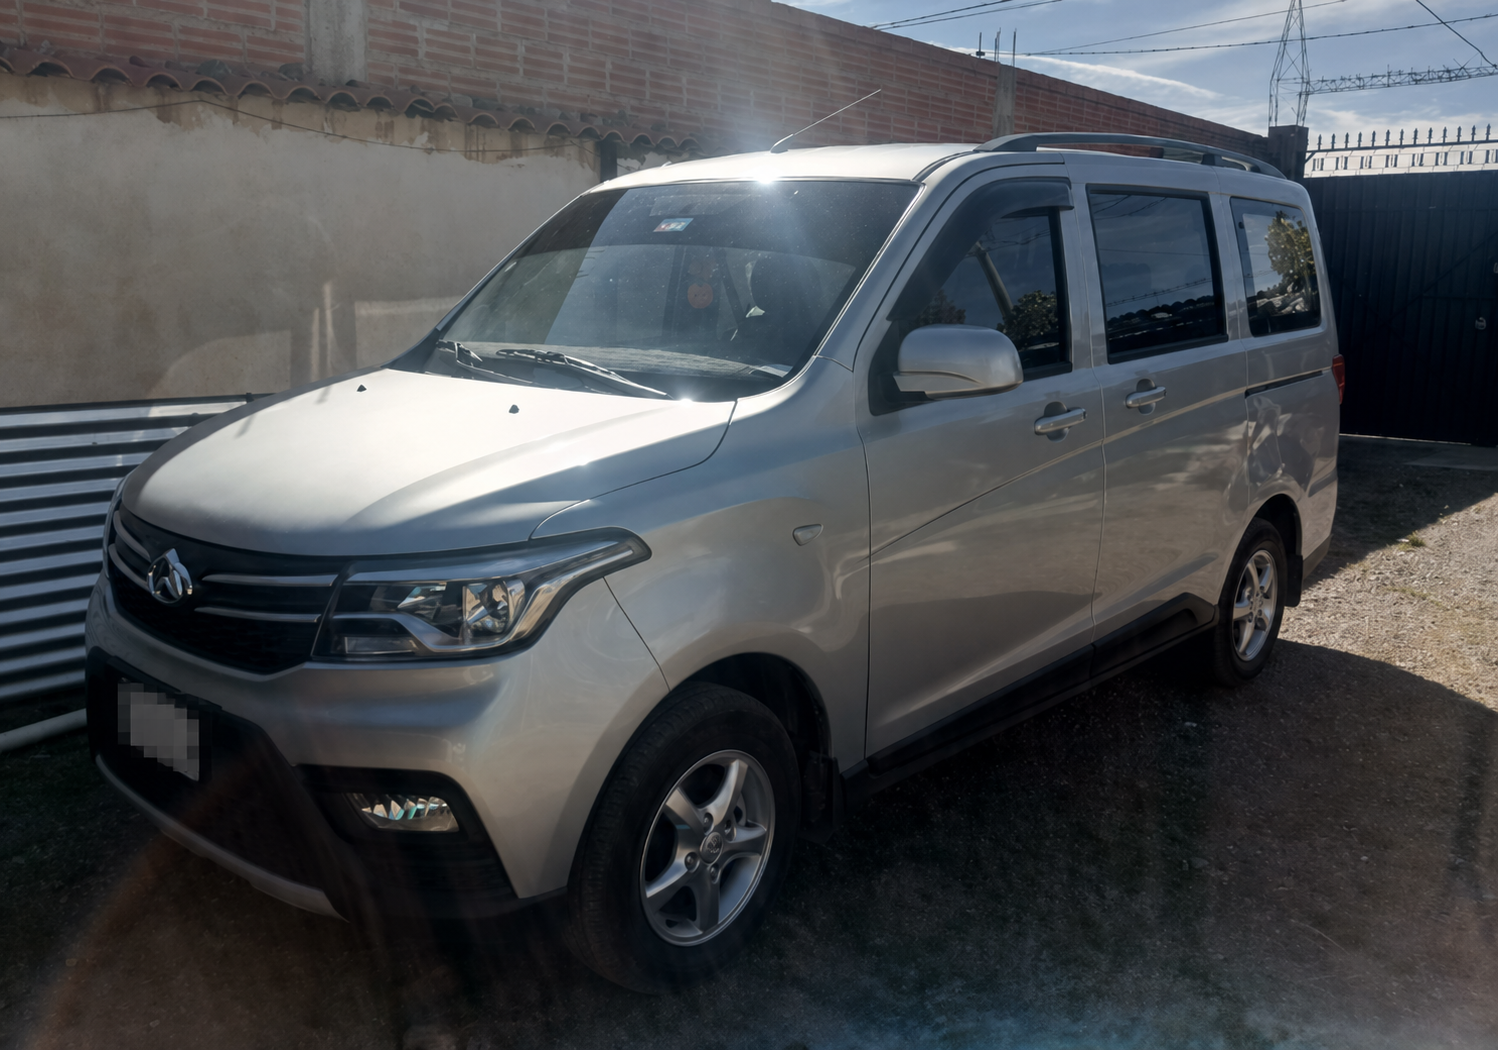
\includegraphics[width=\textwidth]{Images/changan.png}
		\caption{Changan Honor (2023)}
		\label{fig:foto_changan}
	\end{subfigure}
	\hfill
	\begin{subfigure}[t]{0.48\textwidth}
		\centering
		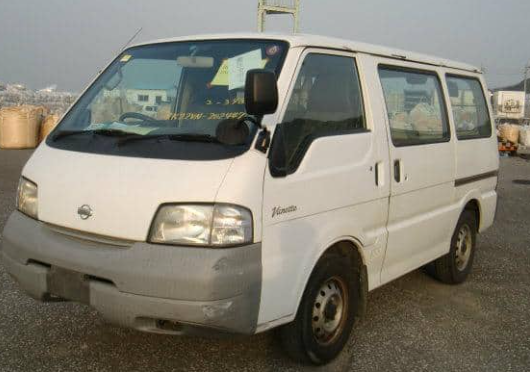
\includegraphics[width=\textwidth]{Images/vanette.png}
		\caption{Nissan Vanette (2018)}
		\label{fig:foto_vanette}
	\end{subfigure}
	\vspace{2pt}
	\\
	{\footnotesize\textit{Nota.} Placa del Changan Honor cubierta por privacidad. Elaboración propia.}
\end{figure}

\subsection{Configuración del adaptador ELM327 como referencia de validación}
\label{sec:elm327_ref}

El adaptador comercial ELM327 (Figura~\ref{fig:elm327_bluetooth}) se emplea como dispositivo de referencia para validar el correcto funcionamiento y la adquisición de datos del sistema desarrollado. Debido a su amplia difusión en la decodificación de protocolos OBD-II, este adaptador permite contrastar las lecturas de los parámetros del motor en tiempo real obtenidos por el prototipo propuesto. Para las pruebas de campo, el ELM327 se configura en modo de comunicación Bluetooth, forzando la selección del protocolo ISO 15765-4 (CAN a 500\,kbps, ID de 11 bits) de manera manual para optimizar los tiempos de inicialización y evitar el proceso de autodetección en cada conexión.

Como herramienta comercial de evaluación se utiliza la aplicación \textit{Car Scanner ELM OBD2}, la cual procesa la información enviada por el ELM327 para calcular el consumo instantáneo y acumulado a partir de las mismas variables del bus CAN (como las RPM, la presión absoluta del colector de admisión MAP y la velocidad del vehículo).

Conviene precisar que tanto el sistema propuesto como la solución basada en el ELM327 calculan el consumo de combustible mediante estimaciones indirectas (método \textit{Speed-Density}) basadas en las señales recopiladas por el bus CAN, y no mediante una medición de flujo directo de gasolina. Así, el cotejo entre ambos equipos representa una prueba de concordancia entre dos plataformas de decodificación.

\textit{Limitación de conexión simultánea.} En las pruebas de campo se verificó que el sistema propio y el adaptador ELM327 no pueden mantener ambos una comunicación estable con la ECU del vehículo al conectarse al mismo tiempo al puerto OBD-II: únicamente uno de los dos dispositivos logra establecer y sostener la sesión de diagnóstico. En consecuencia, la comparación entre ambos no se realiza sobre una única sesión simultánea, sino recorriendo el mismo trayecto dos veces de forma consecutiva (primero con el sistema propio conectado en solitario y, luego, inmediatamente después, con el ELM327 en solitario), manteniendo en lo posible las mismas condiciones de tráfico, ruta y estilo de conducción entre ambas pasadas. Esto introduce una fuente adicional de variabilidad entre las dos lecturas que no proviene de los instrumentos en sí, sino de la imposibilidad de repetir exactamente el mismo tránsito dos veces; se documenta aquí como una limitación metodológica explícita del estudio. Para obtener una referencia de consumo que no dependa de esta limitación ni de ningún método de estimación electrónica, las lecturas de ambos dispositivos se complementan con mediciones volumétricas directas mediante el método de tanque lleno a tanque lleno (Sección~\ref{sec:protocolo_tanque}), realizadas con el sistema propio conectado de forma continua durante todo el trayecto real, tal como se detalla en la Sección~\ref{sec:validacion_cuantitativa}.

% --- FIGURA DE REFERENCIA DEL ELM327 ---
\begin{figure}[htbp]
	\centering
	\caption{Adaptador comercial ELM327 Bluetooth utilizado para la validación de lecturas OBD-II.}
	\label{fig:elm327_bluetooth}
	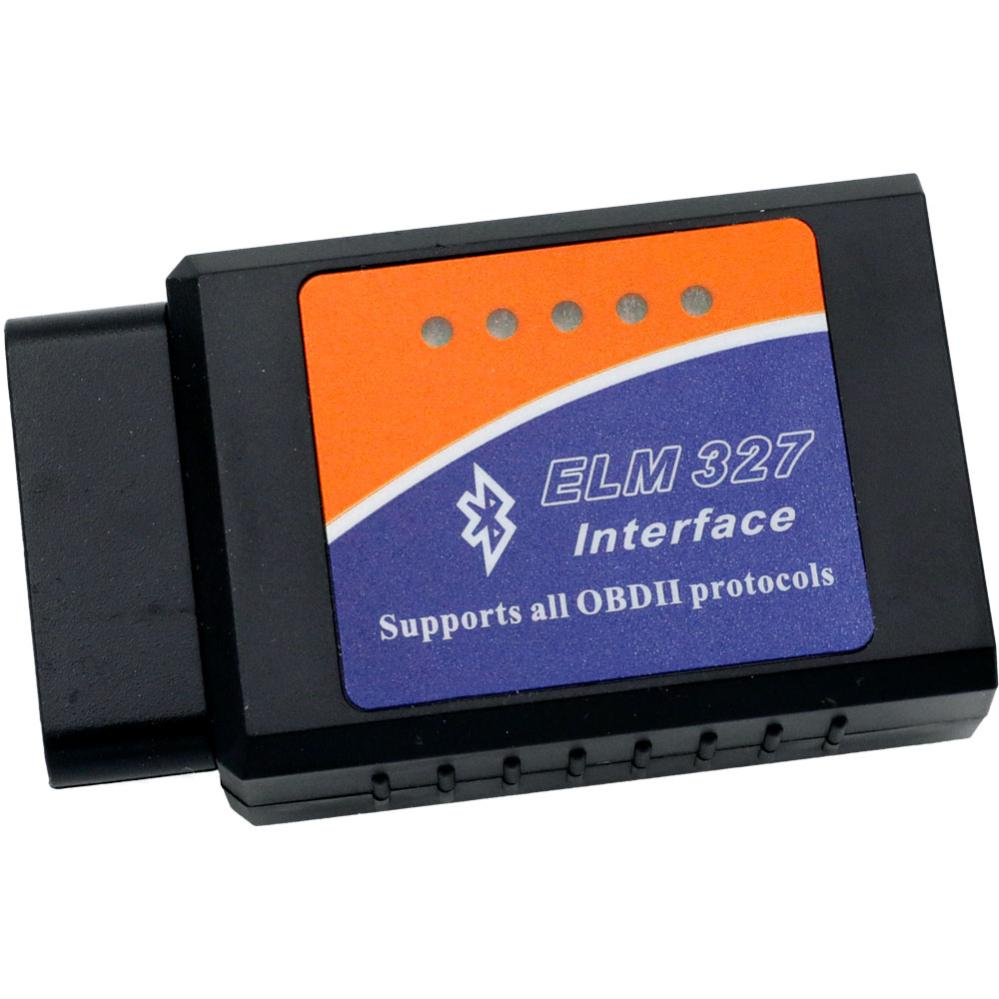
\includegraphics[width=0.45\textwidth]{Images/elm327.jpg} % Ajusta la ruta y nombre de tu imagen
	\\
	\vspace{2pt}
	{\footnotesize\textit{Nota.} Scanner comercial ELM327.}
\end{figure}

\subsection{Puesta en marcha del firmware y verificación inicial}

Antes de cada sesión de pruebas, se ejecuta una rutina de verificación inicial que confirma la correcta inicialización del controlador TWAI (sin errores de bus-off), el montaje del sistema de archivos en la tarjeta MicroSD, la sincronización horaria del registro de datos y la visualización de al menos un parámetro en tiempo real (RPM o velocidad) en la pantalla OLED. La confirmación del correcto funcionamiento de cada uno de estos subsistemas se realiza mediante indicadores LED integrados en el módulo (Tabla~\ref{tab:checklist_arranque}); así se descarta en segundos una falla de montaje antes de invertir tiempo de trayecto en una sesión de prueba inválida.

\begin{table}[H]
	\centering
	\captionsetup{labelformat=simple, labelsep=newline, textfont=it, labelfont=bf, justification=raggedright, singlelinecheck=false}
	\caption{Lista de verificación previa a cada sesión de pruebas}
	\label{tab:checklist_arranque}
	\begin{tabularx}{\textwidth}{>{\raggedright\arraybackslash}p{4.2cm} X >{\centering\arraybackslash}p{2.6cm}}
		\toprule
		\rowcolor[rgb]{0.851, 0.851, 0.851}
		Verificación & Indicador esperado & Resultado \\
		\midrule
		Bus CAN inicializado, sin bus-off & LED CAN encendido fijo tras conectar el contacto & \checkmark \\
		Tarjeta MicroSD montada & LED SD parpadea al escribir (una vez por segundo) &\checkmark \\
		Servidor web activo & LED Server encendido; SSID \texttt{ESP32\_OBD2} visible al buscar redes &\checkmark \\
		Ningún error activo & LED Error apagado (sin patrón de parpadeo) & \checkmark \\
		Parámetro en vivo visible & RPM o velocidad actualizándose en el OLED & \checkmark \\
		\bottomrule
	\end{tabularx}
	\vspace{2mm}
	\\
	\begin{minipage}{\linewidth}
		\small
		\textit{Nota.} Se completa con \checkmark~(correcto) o \texttt{X} (falla, con la causa anotada aparte) al inicio de cada sesión, antes de arrancar el vehículo. Si el LED de error está encendido, el código de parpadeo (Sección~4.3 del Capítulo~3, \texttt{status\_leds.cpp}) indica el subsistema que falló.
	\end{minipage}
\end{table}

\subsection{Herramientas y procesamiento de datos para el análisis}
\label{sec:herramientas_analisis}

Cada sesión de prueba produce datos de tres fuentes distintas, que deben combinarse fuera del dispositivo para calcular las métricas de la Sección~\ref{sec:validacion_cuantitativa}:

\begin{enumerate}
	\item \textbf{CSV del sistema propio}, descargado desde el panel web (\texttt{/api/download}) al finalizar cada trayecto, o directamente de la tarjeta MicroSD. Contiene una fila por segundo con las columnas descritas en el Capítulo~3 (\texttt{trip\_km}, \texttt{trip\_fuel\_L}, \texttt{instant\_L100km}, \texttt{baro\_kpa}, entre otras).
	\item \textbf{Registro del ELM327 + \textit{Car Scanner}}, exportado como CSV o KML/GPX desde la propia aplicación (opción de exportación en el historial de sesión), con marcas de tiempo y consumo instantáneo/acumulado calculado por la app.
	\item \textbf{Bitácora manual de aforo}, un cuaderno o planilla con hora, odómetro y litros cargados en cada llenado de tanque (Sección~\ref{sec:protocolo_tanque}).
\end{enumerate}

El análisis se centraliza en un script de Python (\texttt{pandas} para leer y alinear los CSV por marca de tiempo, \texttt{numpy}/\texttt{scipy.stats} para las métricas estadísticas) en vez de calcularse a mano: de esta forma el proceso es reproducible, permite reprocesar todos los trayectos si se detecta un error, y deja un registro auditable de exactamente cómo se obtuvo cada número de la Tabla~\ref{tab:metricas_validacion}. Este y el resto de los scripts de análisis usados en el capítulo se encuentran en la carpeta \texttt{CODIGOS/} del repositorio de GitHub del proyecto \citep{CalleGitHub2026}, junto con el firmware del dispositivo. Las funciones utilizadas para cada métrica son las siguientes:

\begin{itemize}
	\item RMSE y MAE: \texttt{numpy.sqrt(numpy.mean((est-ref)**2))} y \texttt{numpy.mean(numpy.abs(est-ref))} respectivamente, sobre los pares (estimado, referencia) de cada trayecto o punto de muestreo.
	\item MAPE: \texttt{numpy.mean(numpy.abs((est-ref)/ref))*100}, evitando dividir entre valores de referencia cercanos a cero (por ejemplo, excluyendo muestras con el vehículo detenido).
	\item Pearson $r$ y $R^2$: \texttt{scipy.stats.pearsonr(est, ref)}; $R^2$ es el cuadrado del coeficiente devuelto, o directamente el de una regresión lineal con \texttt{scipy.stats.linregress}.
	\item Bland-Altman: calcular por muestra la diferencia $d = est - ref$ y el promedio $m = (est+ref)/2$; el sesgo medio es $\bar d$ y los límites de concordancia son $\bar d \pm 1{,}96\,s_d$, con $s_d$ la desviación estándar de $d$. Un gráfico de dispersión de $d$ contra $m$, con esas tres líneas horizontales, es la figura estándar de este análisis.
	\item Repetibilidad: coeficiente de variación $CV = s/\bar{x}$ del sistema propio sobre las repeticiones del mismo trayecto (Sección~\ref{sec:protocolo_tanque}), expresado en porcentaje.
\end{itemize}

\section{Pruebas experimentales}

Esta sección describe la metodología seguida para cada tipo de prueba. En todos los casos se recomienda repetir cada prueba al menos 3 veces para poder estimar la variabilidad de la medición y no depender de una sola observación.

\subsection{Validación de la comunicación CAN (ESP32 vs. ELM327)}

Esta prueba verifica que el sistema propuesto decodifica correctamente las tramas de la ECU, con una tasa de éxito comparable a la del adaptador comercial. Dado que, como se explicó en la Sección~\ref{sec:elm327_ref}, ambos dispositivos no pueden mantener una sesión OBD-II estable conectados simultáneamente al mismo puerto, esta verificación se realiza en dos sesiones separadas y consecutivas —motor encendido en ralentí, ventana de tiempo fija (por ejemplo, 5 minutos) para cada dispositivo—, registrando el número de tramas recibidas, la tasa de tramas perdidas o corruptas, y la latencia entre solicitud y respuesta de cada uno por separado. La Tabla~\ref{tab:validacion_can} propone el formato de registro; la columna ``Diferencia'' compara el desempeño de cada dispositivo en su propia sesión, no una medición conjunta.

\begin{table}[H]
	\centering
	\captionsetup{labelformat=simple, labelsep=newline, textfont=it, labelfont=bf, justification=raggedright, singlelinecheck=false}
	\caption{Formato de registro para la validación de la comunicación CAN (sesiones separadas)}
	\label{tab:validacion_can}
	\begin{tabularx}{\textwidth}{X >{\centering\arraybackslash}p{3.5cm} >{\centering\arraybackslash}p{2.5cm} >{\centering\arraybackslash}p{2.5cm}}
		\toprule
		\rowcolor[rgb]{0.851, 0.851, 0.851}
		Parámetro & ESP32-S3 (sesión propia) & ELM327 (sesión separada) & Diferencia \\
		\midrule
		Tramas recibidas en 5 min & 2936 & 1712 & 1224 \\
		Tramas con error de CRC & 0 & 34 & 34 \\
		Latencia promedio (ms) & 2.2 & 231.4 & 229.2 \\
		\bottomrule
	\end{tabularx}
	\vspace{2mm}
	\\
	\begin{minipage}{\linewidth}
		\small
		\textit{Nota.} Cada columna de dispositivo corresponde a una sesión de conexión independiente (Sección~\ref{sec:elm327_ref}), con el vehículo en ralentí para minimizar la variabilidad entre ambas ventanas de medición.
	\end{minipage}
\end{table}

\subsubsection*{Herramientas de medición}

Los valores de la Tabla~\ref{tab:validacion_can} se obtuvieron con dos programas de referencia construidos específicamente para esta prueba, uno por dispositivo, ya que ninguno de los dos expone estas métricas de forma nativa:

\begin{itemize}
	\item \textbf{ESP32-S3} (\texttt{CODIGOS/can\_bench\_tool/}): un proyecto PlatformIO independiente del firmware de producción que, durante 5~minutos, solicita repetidamente el PID~0x0C (RPM), el único PID obligatorio en todo ECU OBD-II (así se aísla el desempeño de la comunicación en sí de la disponibilidad de un PID particular), y mide el tiempo entre cada solicitud y su respuesta directamente sobre el controlador TWAI nativo.
	\item \textbf{ELM327} (\texttt{CODIGOS/elm327\_bench.py}): un script en Python que se conecta al adaptador por Bluetooth y le envía el mismo PID mediante comandos AT estándar, sin pasar por la aplicación comercial, para medir la misma ventana de 5~minutos bajo las mismas condiciones de solicitud.
\end{itemize}

\begin{figure}[H]
	\centering
	\caption{Núcleo de medición de latencia en el benchmark del ESP32-S3, \texttt{can\_bench\_tool/src/main.cpp}.}
	\label{fig:bench_esp32}
	\begin{lstlisting}[language=C++, basicstyle=\fontsize{9}{10}\ttfamily, breaklines=true]
uint32_t reqStartUs = micros();
requestsSent++;

if (sendPidRequest(PID_TO_TEST) && waitForResponse(PID_TO_TEST, RESPONSE_TIMEOUT_MS)) {
  responsesOk++;
  latencySumUs += (uint64_t)(micros() - reqStartUs);
}

uint32_t alerts = 0;
if (twai_read_alerts(&alerts, 0) == ESP_OK && alerts != 0) {
  if (alerts & (TWAI_ALERT_BUS_ERROR | TWAI_ALERT_ERR_PASS | TWAI_ALERT_BUS_OFF)) {
    errorFrames++;
  }
}
	\end{lstlisting}
	\begin{minipage}{\linewidth}
		\small
		\textit{Nota.} La latencia se mide con \texttt{micros()} entre el envío de la solicitud y la recepción de la trama de respuesta válida; los errores se cuentan a partir de las alertas del propio controlador TWAI (\texttt{ESP-IDF}), no de una re-implementación manual de detección de errores de bus.
	\end{minipage}
\end{figure}

\begin{figure}[H]
	\centering
	\caption{Núcleo de medición y clasificación de respuestas en el benchmark del ELM327, \texttt{elm327\_bench.py}.}
	\label{fig:bench_elm327}
	\begin{lstlisting}[language=Python, basicstyle=\fontsize{9}{10}\ttfamily, breaklines=true]
t0 = time.time()
ser.reset_input_buffer()
ser.write(b"010C\r")
requests_sent += 1

resp = ser.read(64).decode(errors="ignore")
elapsed = time.time() - t0
resp_clean = resp.replace("\r", " ").upper()

if "NO DATA" in resp_clean or "ERROR" in resp_clean or "BUS" in resp_clean:
    error_frames += 1
elif "41 0C" in resp_clean:
    responses_ok += 1
    latencies.append(elapsed)
	\end{lstlisting}
	\begin{minipage}{\linewidth}
		\small
		\textit{Nota.} La latencia incluye, a diferencia de la medición del ESP32-S3, el tiempo de procesamiento interno del ELM327 (traducción de comandos AT a tramas CAN) y de la pila Bluetooth del sistema operativo, no solo el tiempo de bus.
	\end{minipage}
\end{figure}

\subsection{Verificación de comunicación OBD-II mediante PIDs}

La verificación de la comunicación con cada vehículo 
se realizó mediante la solicitud y recepción de 
parámetros estándar definidos por el protocolo 
OBD-II (SAE J1979), conocidos como \textit{Parameter 
	IDs} (PIDs), utilizando el modo de servicio 
\texttt{0x01} (datos en tiempo real).

El procedimiento consistió en enviar tramas CAN 
con el formato estándar OBD-II (\texttt{0x7DF} 
como ID de solicitud broadcast) y capturar la 
respuesta de la ECU de cada vehículo 
(\texttt{0x7E8}). Los PIDs reportados como disponibles por cada 
vehículo fueron contrastados contra la tabla 
de referencia del modo 01 (Apéndice A) 
y el análisis matemático de resolución por PID 
disponible, obteniendo los 
resultados de disponibilidad resumidos en la 
Tabla~\ref{tab:pids_verificacion}, un detalle mas completo se presenta en el Apéndice O.

\begin{table}[H]
	\centering
	\caption{PIDs consultados y disponibilidad por vehículo.}
	\label{tab:pids_verificacion}
	\begin{tabular}{clccc}
		\toprule
		\rowcolor[rgb]{.851,.851,.851}
		\textbf{PID} & \textbf{Parámetro} & \textbf{Unidad} & \textbf{Changan Honor} & \textbf{Nissan Vanette} \\
		\midrule
		\texttt{0x0C} & Régimen del motor (RPM) & rpm & \checkmark & \checkmark \\
		\texttt{0x0D} & Velocidad del vehículo & km/h & \checkmark & \checkmark \\
		\texttt{0x10} & Flujo másico de aire (MAF) & g/s &  & \checkmark \\
		\texttt{0x05} & Temperatura del refrigerante & °C & \checkmark & \checkmark \\
		\texttt{0x11} & Posición del acelerador & \% & \checkmark & \checkmark \\
		\bottomrule
	\end{tabular}
	\vskip 0.15cm
	{\footnotesize \textit{Nota.} PIDs verificados mediante el escaneo de la Figura~\ref{fig:codigo_scanner_obd2}.}
\end{table}

La disponibilidad del PID \texttt{0x10} (MAF) 
en ambos vehículos es crítica para el sistema,
ya que es el parámetro base para el
cálculo del consumo de combustible, conforme
a la fórmula de decodificación definida por 
el estándar SAE J1979 \citep{saej1979}.

\subsection{Pruebas del modelo Speed-Density}

Se realizan pruebas estáticas a régimen de motor controlado (en ralentí y en pasos de 1500, 2500 y 3500\,rpm, sin carga en las ruedas) con el fin de aislar el comportamiento del modelo Speed-Density de las variables dinámicas de conducción. El primer punto no se fija a un número redondo arbitrario (por ejemplo, 800\,rpm): el regulador de ralentí de cada motor tiene su propio piso, por debajo del cual el motor no puede sostenerse sin calarse —en el Nissan Vanette utilizado, ese piso se ubicó experimentalmente entre 960 y 980\,rpm—, así que el primer punto se toma directamente como el ralentí real medido al inicio de la prueba. En cada punto se registra el caudal de aire estimado por el sistema propio y se contrasta contra el valor de referencia reportado por la ECU a través del PID estándar de MAF, cuando el vehículo lo soporta.

Esta comparación directa punto a punto solo es posible en el \textbf{Nissan Vanette}, que sí reporta el PID 0x10 (Tabla~\ref{tab:pids_verificacion}). El \textbf{Changan Honor} no dispone de sensor MAF (es, de hecho, la razón por la que este proyecto necesita el método Speed-Density en primer lugar, Sección~\ref{subsec:soporte_pids} del Capítulo~3), de modo que no existe una referencia directa de caudal de aire para ese vehículo en esta prueba estática. Su exactitud se evalúa entonces de forma indirecta, aguas abajo, a través de la comparación de consumo acumulado contra el aforo real por tanque lleno (Sección~\ref{sec:protocolo_tanque}), que sí aplica a ambos vehículos por igual.

\subsubsection*{Herramienta de medición}

A diferencia de la validación de comunicación CAN de la sección anterior, esta prueba no compara un dispositivo contra otro, sino una \emph{estimación} contra una \emph{referencia}, y ambas se calculan a partir de las mismas lecturas de RPM, MAP e IAT tomadas en el mismo instante. Por eso aquí basta con el \textbf{ELM327 solo}, hablado directamente por un script en Python (\texttt{CODIGOS/speed\_density\_bench.py} en el repositorio del proyecto \citep{CalleGitHub2026}): en cada ciclo solicita RPM (PID~0x0C), MAP (PID~0x0B), IAT (PID~0x0F) y MAF real (PID~0x10), y con las tres primeras calcula el MAF estimado usando exactamente la misma fórmula y tabla de eficiencia volumétrica (VE) que el firmware de producción (\texttt{fuel\_calc.cpp}). Al no requerir una segunda sesión OBD-II en paralelo, esta prueba queda al margen de la limitación de conexión simultánea documentada en la Sección~\ref{sec:elm327_ref}.

\begin{figure}[H]
	\centering
	\caption{Cálculo del MAF estimado en \texttt{speed\_density\_bench.py}, réplica en Python de la fórmula de \texttt{fuel\_calc.cpp}.}
	\label{fig:bench_speed_density}
	\begin{lstlisting}[language=Python, basicstyle=\fontsize{9}{10}\ttfamily, breaklines=true]
def maf_estimado_gs(rpm, map_kpa, iat_c):
    ve = ve_for_rpm(rpm)          # misma tabla VE que kVeTable en fuel_calc.cpp
    iat_k = iat_c + 273.15
    if iat_k < 233.15 or iat_k > 373.15:
        iat_k = 288.15             # misma guarda que el firmware
    maf = (ve / 100.0) * rpm * map_kpa * ENGINE_DISPLACEMENT_L * MM_AIR \
          / (2.0 * R * iat_k * 60.0)
    return max(maf, 0.0)
	\end{lstlisting}
	\begin{minipage}{\linewidth}
		\small
		\textit{Nota.} \texttt{ENGINE\_DISPLACEMENT\_L}, la tabla \texttt{VE\_TABLE} y las constantes \texttt{MM\_AIR}/\texttt{R} son una copia literal de los valores de \texttt{config.h} y \texttt{fuel\_calc.cpp}, de modo que la estimación calculada en la prueba es la misma que produciría el equipo embarcado ante las mismas lecturas.
	\end{minipage}
\end{figure}

Al iniciar, el script mide el ralentí real promediando varias lecturas de RPM antes de comenzar a clasificar muestras, y lo antepone a los otros tres puntos fijos (1500, 2500 y 3500~rpm) como el primer objetivo de la prueba. Cada muestra se clasifica según el punto de régimen objetivo más cercano, con tolerancia de $\pm$100~rpm, y se descarta si no cae dentro de esa tolerancia; al finalizar la prueba el script promedia el MAF estimado y el MAF de referencia dentro de cada punto y calcula el error porcentual entre ambos.

\begin{table}[H]
	\centering
	\caption{Comparación del MAF estimado por el modelo Speed-Density frente al MAF de referencia de la ECU (PID 0x10), Nissan Vanette}
	\label{tab:speed_density_resultados}
	\begin{tabular}{ccccc}
		\toprule
		\rowcolor[rgb]{0.851, 0.851, 0.851}
		\textbf{RPM} & \textbf{n muestras} & \textbf{MAF estimado (g/s)} & \textbf{MAF ref. (g/s)} & \textbf{Error (\%)} \\
		\midrule
		Ralentí (940\,rpm) & 22 & 2,04 & 2,68 & $-23{,}7$ \\
		1500 & 25 & 3,52 & 3,90 & $-9{,}8$ \\
		2500 & 22 & 7,21 & 6,89 & $+4{,}7$ \\
		3500 & 20 & 11,74 & 9,90 & $+18{,}7$ \\
		\bottomrule
	\end{tabular}
	\vskip 0.15cm
	{\footnotesize \textit{Nota.} Valores promedio por punto de régimen, obtenidos con \texttt{speed\_density\_bench.py} y registrados en \texttt{speed\_density\_log.csv}. Error (\%) = (MAF estimado $-$ MAF referencia) / MAF referencia $\times$ 100.}
\end{table}

\begin{figure}[H]
	\centering
	\caption{Comparación del caudal de aire estimado por el modelo Speed-Density frente al valor de referencia de la ECU, por régimen de motor}
	\label{fig:speed_density_scatter}
	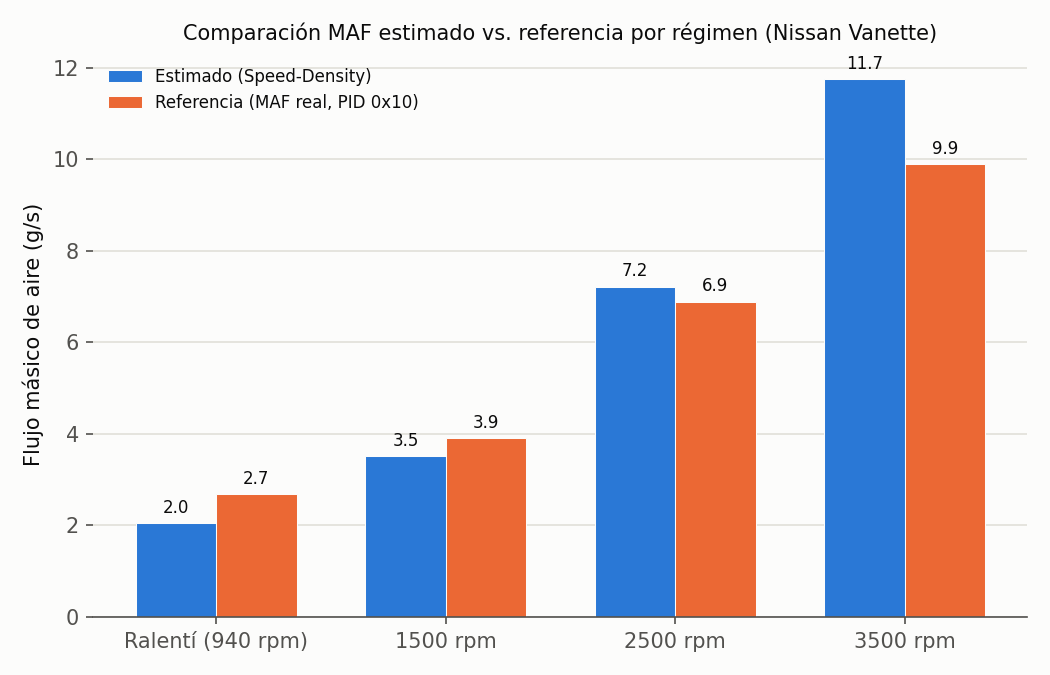
\includegraphics[width=0.8\textwidth]{Images/figura_4_9_speed_density.png}

	\vspace{2pt}
	{\footnotesize\textit{Nota.} Gráfico de barras agrupadas, un par de barras (estimado / referencia) por cada uno de los cuatro regímenes evaluados. Se prefiere sobre un diagrama de dispersión porque el diseño experimental produce cuatro promedios discretos por punto de régimen, no una nube de muestras continuas cuya correlación interese visualizar: precisamente el caso de uso de las barras agrupadas frente a la dispersión. Elaboración propia.}
\end{figure}

\subsubsection*{Calibración del modelo Speed-Density}
\label{sec:calibracion_speed_density}

Los resultados de la Tabla~\ref{tab:speed_density_resultados} muestran un error grande y, más importante, de \emph{signo variable} entre regímenes: el modelo subestima el caudal de aire en ralentí y a 1500\,rpm ($-23{,}7\,\%$ y $-9{,}8\,\%$), pero lo sobrestima a 2500 y 3500\,rpm ($+4{,}7\,\%$ y $+18{,}7\,\%$). Un sesgo de signo constante podría explicarse por un solo factor de escala mal calibrado (por ejemplo, la cilindrada); un sesgo que cambia de signo con el régimen, en cambio, apunta a que la \emph{forma} de la curva de eficiencia volumétrica (VE) usada por el modelo no corresponde a la de este motor en particular. Al notar un error de esta magnitud, se procede a calibrar el sistema con los mismos datos de la Tabla~\ref{tab:speed_density_resultados}, en vez de aceptar la tabla VE genérica con la que partió el diseño.

La revisión encontró además un segundo problema, independiente del anterior: la constante \texttt{ENGINE\_DISPLACEMENT\_L} del firmware (\texttt{config.h}) estaba fijada en 1,6\,L, mientras que la cilindrada real del Nissan Vanette, según su ficha técnica (Tabla~\ref{tab:vehiculos}), es de 1626\,mL. Ambas correcciones —cilindrada real y tabla VE calibrada— se aplican juntas antes de recalcular.

\paragraph{Método de calibración.} La ecuación de \texttt{fuel\_calc.cpp} (Sección~\ref{sec:speeddensity} del Capítulo~3) se invierte algebraicamente para despejar la VE que, dada una muestra real de RPM, MAP e IAT, hace que el MAF estimado coincida exactamente con el MAF de referencia:

\begin{equation}
	VE_{\text{requerida}} = \frac{MAF_{\text{ref}} \cdot 100 \cdot 2 \cdot R \cdot T_{IAT} \cdot 60}{RPM \cdot P_{MAP} \cdot V_d \cdot 28{,}97}
	\label{eq:ve_calibracion}
\end{equation}

Esta inversión se aplica muestra por muestra sobre \texttt{speed\_density\_log.csv} y se promedia por punto de régimen mediante \texttt{CODIGOS/calibrate\_ve\_table.py}, un script nuevo e independiente de \texttt{speed\_density\_bench.py} (no requiere el vehículo ni el ELM327, solo el CSV ya grabado). La Tabla~\ref{tab:ve_calibracion} resume la VE que exigía la tabla genérica original frente a la VE real requerida en cada punto.

\begin{table}[H]
	\centering
	\caption{Eficiencia volumétrica (VE) genérica frente a la VE real requerida, por punto de régimen}
	\label{tab:ve_calibracion}
	\begin{tabular}{cccc}
		\toprule
		\rowcolor[rgb]{0.851, 0.851, 0.851}
		\textbf{Punto} & \textbf{RPM promedio real} & \textbf{VE genérica (\%)} & \textbf{VE requerida (\%)} \\
		\midrule
		Ralentí & 936,3 & 64,1 & 82,7 \\
		1500    & 1446,7 & 73,1 & 79,7 \\
		2500    & 2491,6 & 84,9 & 79,7 \\
		3500    & 3483,0 & 87,0 & 72,7 \\
		\bottomrule
	\end{tabular}
	\vskip 0.15cm
	{\footnotesize \textit{Nota.} Calculado con \texttt{calibrate\_ve\_table.py} sobre \texttt{speed\_density\_log.csv}, usando $V_d=1{,}626$\,L. Los puntos 4000/5500/7000\,rpm de \texttt{kVeTable} no se modifican por no contar con datos de prueba en ese rango; quedan documentados como sin calibrar.}
\end{table}

La tabla \texttt{kVeTable} de \texttt{fuel\_calc.cpp} y su copia en \texttt{speed\_density\_bench.py} se actualizan con estos cuatro puntos calibrados, conservando sin cambios los tres puntos superiores (4000/5500/7000\,rpm) por no contarse con mediciones reales en ese rango.

\begin{figure}[H]
	\centering
	\caption{Validación de la tabla VE calibrada frente al MAF de referencia, mismo conjunto de datos de calibración}
	\label{fig:post_calibracion}
	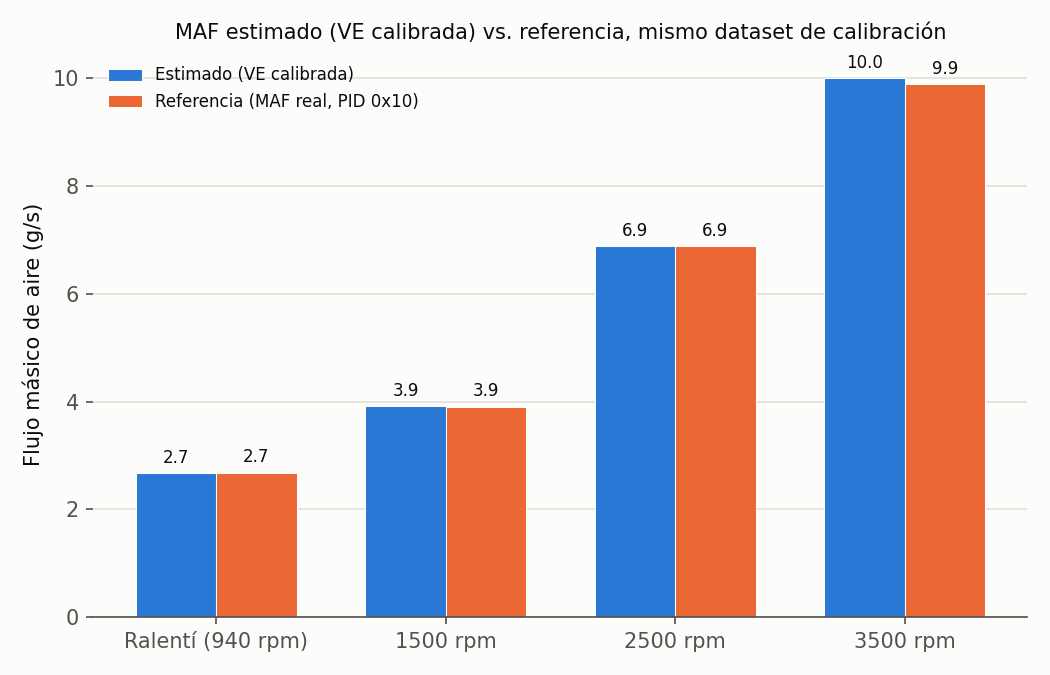
\includegraphics[width=0.8\textwidth]{Images/figura_4_10_post_calibracion.png}

	\vspace{2pt}
	{\footnotesize\textit{Nota.} Generado por \texttt{calibrate\_ve\_table.py} recalculando el MAF estimado de cada muestra con la tabla ya calibrada. El error residual (entre $-0{,}02\,\%$ y $+1{,}03\,\%$ según el punto) confirma que la inversión algebraica se aplicó correctamente, pero \textbf{no} es una validación independiente del modelo: al calibrar y verificar sobre el mismo conjunto de datos, un error cercano a cero es el resultado esperado por construcción, no evidencia de que el modelo generalice a condiciones dinámicas de conducción o a otro rango de régimen. Elaboración propia.}
\end{figure}

Esta limitación metodológica —validar sobre el mismo conjunto de datos con el que se calibró— se resuelve con una segunda prueba, dinámica, descrita a continuación.

\subsubsection*{Prueba dinámica (ruta real)}
\label{sec:sd_prueba_dinamica}

A diferencia de la prueba estática anterior, aquí no se sostiene el motor en puntos fijos de régimen: se conduce una ruta real (arranque, aceleración, crucero a distintas velocidades, frenado) mientras el sistema registra continuamente RPM, MAP, IAT y el MAF real de referencia. El objetivo no es calibrar nada —la tabla VE ya quedó fija en la prueba estática—, sino verificar qué tan bien predice el modelo \emph{ya calibrado} sobre datos que nunca participaron en esa calibración, resolviendo directamente la limitación señalada en la Figura~\ref{fig:post_calibracion}. Al igual que la prueba estática, esta solo aplica al \textbf{Nissan Vanette} (único vehículo con PID 0x10).

\texttt{CODIGOS/speed\_density\_drive\_log.py} realiza este registro: a diferencia de \texttt{speed\_density\_bench.py}, no agrupa las muestras por punto de régimen objetivo ni corta automáticamente (ese criterio, pensado para la prueba estática, cortaría una ruta real apenas el RPM de manejo normal pasara cerca de cualquiera de los 4 puntos fijos), así que aquí simplemente registra cada muestra tal como llega, sin requerir ninguna interacción mientras se maneja. Al finalizar (Ctrl+C), \texttt{CODIGOS/speed\_density\_drive\_validation.py} calcula sobre el registro completo las mismas métricas ya definidas en la Sección~\ref{sec:herramientas_analisis} (RMSE, MAE, MAPE, coeficiente de Pearson) y genera un diagrama de dispersión del MAF estimado frente al de referencia. A diferencia de la Figura~\ref{fig:speed_density_scatter} (barras, 4 promedios discretos), aquí sí corresponde un diagrama de dispersión: el registro de una ruta produce una nube continua de muchas muestras correlacionadas, el caso de uso exacto de ese tipo de gráfico.

\begin{figure}[H]
	\centering
	\caption{Dispersión del MAF estimado frente al MAF de referencia durante una ruta real}
	\label{fig:dispersion_dinamica}
	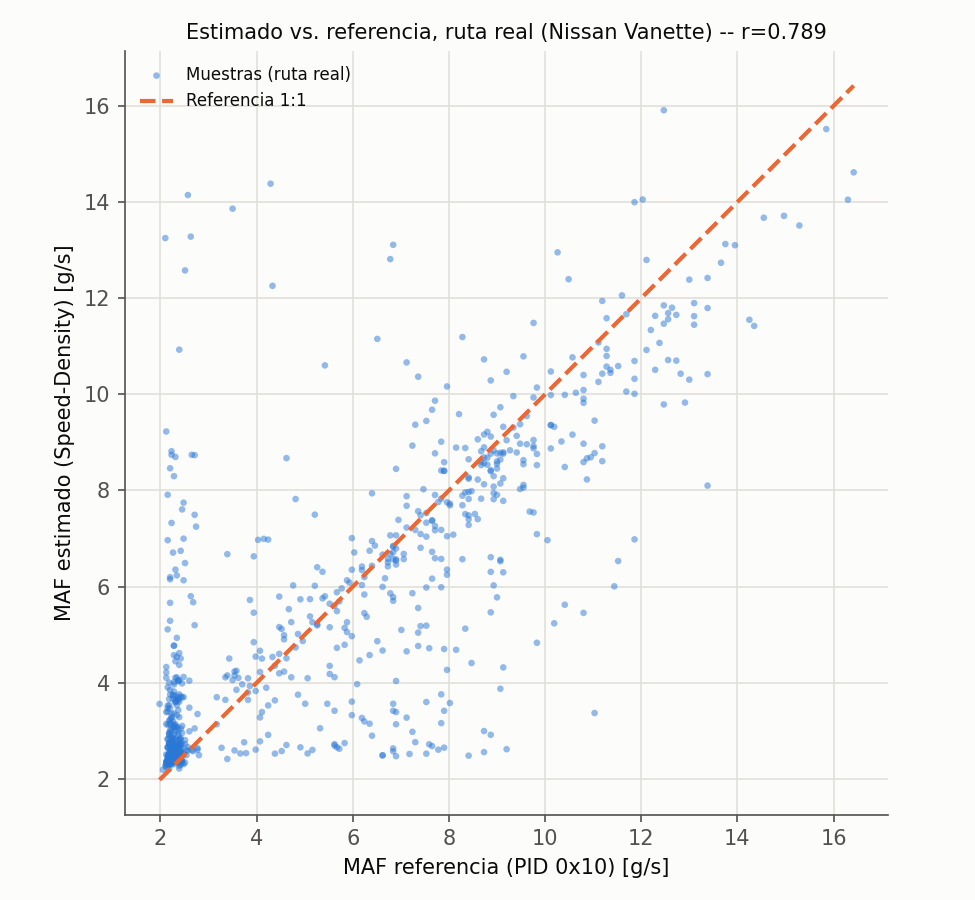
\includegraphics[width=0.7\textwidth]{Images/figura_dispersion_dinamica.png}

	\vspace{2pt}
	{\footnotesize\textit{Nota.} Cada punto es una muestra del registro de ruta; la línea discontinua es la recta 1:1 (predicción perfecta). Elaboración propia.}
\end{figure}

\subsection{Validación del sensor MAP frente a la altitud}
\label{sec:validacion_map_altitud}

A diferencia de una implementación que asumiera una presión de referencia fija
de nivel del mar, el método speed-density de este proyecto usa en cada ciclo
la presión absoluta real del colector (MAP, PID 0x0B) reportada por la propia
ECU, por lo que el cálculo de consumo ya queda corregido por altitud sin
necesitar ningún factor adicional (Sección~\ref{sec:speeddensity} y
Subsección~\ref{subsec:etav-altitud} del Capítulo~3). Lo que sí conviene
verificar en campo es que el \emph{sensor} MAP del vehículo esté bien
calibrado para operar a los $\approx 3\,600$\,msnm de La Paz, ya que un sesgo
de fábrica en ese sensor sí se propagaría al consumo calculado.

La prueba consiste en comparar, con el contacto puesto y el motor apagado
(\textit{key-on, engine-off}, sin vacío de admisión), la lectura de MAP
contra la presión barométrica real. El firmware registra esta última como
\texttt{baro\_kpa} en el CSV y en el panel web (PID 0x33 cuando el vehículo
lo soporta; en su defecto, la estimación del modelo ISA evaluado en
\texttt{SITE\_ALTITUDE\_M}, marcada como tal mediante
\texttt{baro\_is\_estimated}). La Tabla~\ref{tab:validacion_map_altitud}
propone el formato de registro.

\subsubsection*{Herramienta de medición}

Al ser una prueba puntual (motor apagado, sin trayecto de por medio), esta fila de la Tabla~\ref{tab:validacion_map_altitud} se llena con un script independiente, \texttt{CODIGOS/map\_altitude\_report.py}, que se conecta directamente al ELM327 por Bluetooth y no requiere el sistema propio conectado a la vez: solicita el PID~0x0B (MAP) y el PID~0x33 (presión barométrica) un número fijo de veces, promedia ambas lecturas y calcula la diferencia porcentual entre ellas. Si el vehículo no soporta el PID~0x33 —caso que se decide en tiempo de ejecución, no de antemano—, el script recurre al mismo modelo ISA evaluado en \texttt{SITE\_ALTITUDE\_M} que usa el firmware como respaldo (\texttt{isaPressureKpaAt()} en \texttt{can\_obd2.cpp}), replicado con la fórmula idéntica en Python. Cada corrida se ejecuta una vez por vehículo y se anexa a \texttt{map\_altitude\_report.csv}, listo para copiar a la Tabla~\ref{tab:validacion_map_altitud}.

\begin{table}[H]
	\centering
	\captionsetup{labelformat=simple, labelsep=newline, textfont=it, labelfont=bf, justification=raggedright, singlelinecheck=false}
	\caption{Validación del sensor MAP en \textit{key-on, engine-off} frente a la presión barométrica}
	\label{tab:validacion_map_altitud}
	\begin{tabularx}{\textwidth}{X >{\centering\arraybackslash}p{3cm} >{\centering\arraybackslash}p{3cm} >{\centering\arraybackslash}p{3cm}}
		\toprule
		\rowcolor[rgb]{0.851, 0.851, 0.851}
		Vehículo & MAP en KOEO (kPa) & \texttt{baro\_kpa} (kPa) & Diferencia (\%) \\
		\midrule
		Changan Honor & 63.0 & 63.0 & 0.0 \\
		Nissan Vanette & 63.0 & 64.6 & -2.5 \\
		\bottomrule
	\end{tabularx}
	\vspace{2mm}
	\\
	\begin{minipage}{\linewidth}
		\small
		\textit{Nota.} Una diferencia pequeña (idealmente de pocos kPa) confirma que el sensor MAP reporta la presión atmosférica real de La Paz, y con ello que el cálculo speed-density parte de una base correcta; una diferencia grande señalaría un sesgo de calibración del sensor MAP que ninguna corrección de software puede resolver por sí sola.
	\end{minipage}
\end{table}

Como referencia teórica de contraste, el modelo ISA evaluado a
$3\,600$\,msnm predice $P(3\,600) \approx 64{,}9$\,kPa (Capítulo~3,
Ecuación de la Atmósfera Estándar Internacional).

\subsection{Protocolo de trayectos de referencia (tanque lleno a tanque lleno)}
\label{sec:protocolo_tanque}

Esta es la prueba central de la validación (Sección~\ref{sec:validacion_cuantitativa}), ya que produce el único dato de consumo que no depende de ningún método de estimación electrónica: el volumen de combustible efectivamente repuesto. Su valor como referencia depende por completo de la disciplina con la que se ejecute el protocolo de llenado, por lo que se fijan las siguientes reglas antes de iniciar cada trayecto:

\begin{itemize}
	\item \textbf{Llenado de referencia.} Cargar combustible hasta el corte automático de la pistola del surtidor (\textit{primer clic}), sin continuar el llenado manualmente más allá de ese punto; repetir el mismo criterio al cerrar el trayecto. Siempre que sea posible, usar el mismo surtidor o al menos la misma estación de servicio en ambos extremos, para minimizar diferencias de calibración entre bombas.
	\item \textbf{Registro previo al arranque.} Anotar en la bitácora (Sección~\ref{sec:herramientas_analisis}): fecha, hora, odómetro del vehículo, y confirmar que el sistema propio pasó la lista de verificación de la Tabla~\ref{tab:checklist_arranque}.
	\item \textbf{Selección de rutas.} Definir de antemano tres categorías de trayecto por vehículo (corto, medio y largo) para cubrir un rango amplio de distancias y condiciones de manejo (urbano de La Paz y, cuando sea posible, ruta más abierta) en vez de validar el modelo en una única condición. El corto y el medio se repiten 2 veces cada uno, registrando ida y vuelta como tramos separados (4 tramos por categoría); el largo se recorre una sola vez, sin repetición ni separación ida/vuelta.
	\item \textbf{Control del conductor.} Mantener, en la medida de lo posible, el mismo conductor y un estilo de conducción habitual (sin aceleraciones ni frenadas deliberadamente extremas) entre trayectos, de forma que la variabilidad medida refleje principalmente al vehículo y al sistema, no al estilo de manejo.
	\item \textbf{Cierre de cada tramo.} Al final de cada uno de los nueve tramos (corto ida/vuelta $\times$2, medio ida/vuelta $\times$2, largo), registrar odómetro y descargar el CSV del trayecto (\texttt{trip\_km}, \texttt{trip\_fuel\_L}) antes de reiniciar el contador de viaje para el siguiente, \emph{sin} volver a llenar el tanque todavía.
\end{itemize}

A diferencia del planteamiento original de repetir el llenado en cada trayecto, en la práctica no es viable reabastecer en cada uno de los nueve tramos en una sola sesión de pruebas: el llenado de referencia se hace \textbf{una sola vez}, antes del primer tramo (ida del corto) y una vez más al cerrar el último (el largo), de modo que los litros repuestos en ese segundo llenado son el consumo real de referencia de los \textbf{nueve tramos combinados}, no de cada uno por separado. El sistema propio permanece conectado de forma continua durante todos, por lo que sí se puede leer su \texttt{trip\_fuel\_L} individual de cada tramo además del acumulado; la lectura del ELM327 + Car Scanner para cada tramo se obtiene, como en las demás pruebas, en una sesión separada e inmediatamente posterior sobre la misma ruta (Sección~\ref{sec:elm327_ref}). Las Tablas~\ref{tab:comparacion_consumo_vanette} y~\ref{tab:comparacion_consumo_changan} (una por vehículo) y las métricas de la Tabla~\ref{tab:metricas_validacion} comparan el sistema propio contra el ELM327 tramo por tramo, y contra el aforo real solo a nivel del total combinado —única granularidad en la que existe ese dato—, con la variabilidad entre pasadas documentada como limitación metodológica.

\subsection{Pruebas de registro de datos en MicroSD}
\label{sec:pruebas_microsd}

Se verifica la integridad de los archivos generados (formato, ausencia de líneas corruptas o incompletas) tras sesiones de registro de distinta duración, así como el comportamiento del sistema ante una desconexión abrupta de la alimentación durante la escritura, situación habitual al apagar el vehículo.

La prueba consta de dos partes. Primero, se registran al menos dos sesiones de duración claramente distinta (una corta y una larga) para caracterizar el tamaño de archivo y la tasa de muestreo real bajo uso normal; lo que importa no es un número exacto de minutos, sino confirmar que ambos valores se mantienen estables independientemente de la duración de la sesión. Segundo, durante una sesión de registro activa se desconecta la alimentación del sistema de forma abrupta, sin pasar por el apagado ordenado, y se examina el archivo resultante: dado que \texttt{sdLoggerTask()} llama \texttt{flush()} después de cada fila (\texttt{sd\_logger.cpp}), en el peor caso se espera perder únicamente la fila que estaba a medio escribir en el momento del corte, no el archivo completo ni sesiones anteriores. Esta segunda parte es independiente de las duraciones elegidas para la primera.

\subsubsection*{Herramienta de medición}

Ambas partes de la prueba se evalúan con \texttt{validate\_sd\_log.py}, un script que se corre directamente sobre los archivos \texttt{trip\_NNN.csv} ya descargados (desde \texttt{/api/download} o copiados de la tarjeta), sin necesitar ninguna conexión al vehículo ni al ELM327. Por cada archivo, verifica que el encabezado coincida con las 18 columnas de \texttt{sd\_logger.cpp}, cuenta las líneas corruptas o incompletas (número de columnas incorrecto o campos no numéricos) y los huecos de muestreo (saltos en \texttt{uptime\_ms} mayores a 2,5 veces el intervalo nominal de \texttt{SD\_LOG\_INTERVAL\_MS}), y calcula la duración cubierta, la tasa de muestreo real y el tamaño de archivo extrapolado a una hora de registro. Cada archivo analizado se anexa a \texttt{sd\_log\_report.csv}, listo para copiar a la Tabla~\ref{tab:validacion_microsd}.

\begin{table}[H]
	\centering
	\captionsetup{labelformat=simple, labelsep=newline, textfont=it, labelfont=bf, justification=raggedright, singlelinecheck=false}
	\caption{Integridad y tasa de registro de los archivos CSV generados en MicroSD, por sesión}
	\label{tab:validacion_microsd}
	\begin{tabularx}{\textwidth}{X >{\centering\arraybackslash}p{2cm} >{\centering\arraybackslash}p{2.2cm} >{\centering\arraybackslash}p{2.2cm} >{\centering\arraybackslash}p{2cm} >{\centering\arraybackslash}p{2.3cm}}
		\toprule
		\rowcolor[rgb]{0.851, 0.851, 0.851}
		Sesión & Duración & Filas válidas & Filas corruptas & Tasa (Hz) & Tamaño / hora \\
		\midrule
		5 min (nominal)  & 5.2 min & 292 & 0 & 1.004 & 290.3\,KB \\
		60 min (nominal) & 60,8 min & 3649 & 0 & 1,000 & 315,8\,KB \\
		Corte abrupto de alimentación & 60,8 min & 3649 & 0 & 1,000 & --- \\
		\bottomrule
	\end{tabularx}
	\vspace{2mm}
	\\
	\begin{minipage}{\linewidth}
		\small
		\textit{Nota.} Valores obtenidos con \texttt{validate\_sd\_log.py} (Changan Honor). Las filas de 60~min y corte abrupto provienen del mismo archivo (\texttt{trip\_003.csv}: sesión en ralentí, cortada de forma abrupta al final). La tasa y el tamaño por hora varían solo $8{,}8\,\%$ entre la sesión corta y la larga: no dependen, entonces, de la duración de la sesión. Las 0 filas corruptas en ambas confirman que el \texttt{flush()} por fila evita corrupción, salvo la última fila, que ni llega a escribirse.
	\end{minipage}
\end{table}

\subsection{Pruebas del panel de control web (WebSocket/HMI)}
\label{sec:pruebas_panel_web}

Se evalúan tres aspectos del panel: la latencia de actualización (qué tan seguido llegan datos nuevos frente al periodo nominal de envío), la estabilidad de la conexión WebSocket durante sesiones prolongadas, y el comportamiento ante la pérdida temporal de la señal WiFi al alejarse del punto de acceso generado por el ESP32-S3.

\subsubsection*{Herramienta de medición}

El propio panel web se instrumentó para esta prueba (\texttt{web\_server.cpp}), sin alterar su funcionamiento normal: cada vez que llega un mensaje por el WebSocket se registra, en el propio navegador, el intervalo respecto al mensaje anterior; cada reconexión también se cuenta. Dos funciones quedan disponibles desde la consola del navegador (F12) mientras el panel está abierto:

\begin{itemize}
	\item \texttt{wsStatsReport()}: imprime un resumen en el momento (n.° de muestras, media, desviación estándar, mínimo, máximo, reconexiones y duración de la sesión).
	\item \texttt{wsStatsDownload()}: descarga \texttt{ws\_intervals.csv} con todos los intervalos individuales, para analizarlos con \texttt{CODIGOS/ws\_latency\_report.py}, que calcula el resumen estadístico y genera un histograma frente al valor nominal (\texttt{WS\_PUSH\_PERIOD\_MS}~=~500\,ms en \texttt{config.h}).
\end{itemize}

El protocolo tiene tres partes: (1) una sesión con el panel abierto y el vehículo en ralentí, leyendo tanto la latencia de actualización (\texttt{wsStatsDownload()}) como el número de reconexiones acumulado (\texttt{wsStatsReport()}) al final (una sola sesión sirve para ambas, ya que no hay razón para separarlas en dos corridas); (2) alejarse físicamente del vehículo con el dispositivo que muestra el panel, en pasos de distancia crecientes, anotando a qué distancia se pierde la conexión (el indicador ``Enlace: WS'' cambia a ``Enlace: polling'') y si reconecta solo al volver a acercarse.

\begin{table}[H]
	\centering
	\captionsetup{labelformat=simple, labelsep=newline, textfont=it, labelfont=bf, justification=raggedright, singlelinecheck=false}
	\caption{Latencia de actualización del panel web (intervalos entre mensajes WebSocket)}
	\label{tab:latencia_panel}
	\begin{tabularx}{\textwidth}{X >{\centering\arraybackslash}p{2cm} >{\centering\arraybackslash}p{2cm} >{\centering\arraybackslash}p{2cm} >{\centering\arraybackslash}p{2cm} >{\centering\arraybackslash}p{2.3cm}}
		\toprule
		\rowcolor[rgb]{0.851, 0.851, 0.851}
		Nominal (ms) & n muestras & Media (ms) & Desv. (ms) & Mín. (ms) & Máx. (ms) \\
		\midrule
		500 & 945 & 500,0 & 10,0 & 314,9 & 602,0 \\
		\bottomrule
	\end{tabularx}
	\vskip 0.15cm
	{\footnotesize \textit{Nota.} Valores calculados por \texttt{ws\_latency\_report.py} sobre \texttt{ws\_intervals.csv}.}
\end{table}

\begin{figure}[H]
	\centering
	\caption{Distribución del intervalo de actualización del panel web frente al valor nominal}
	\label{fig:histograma_ws}
	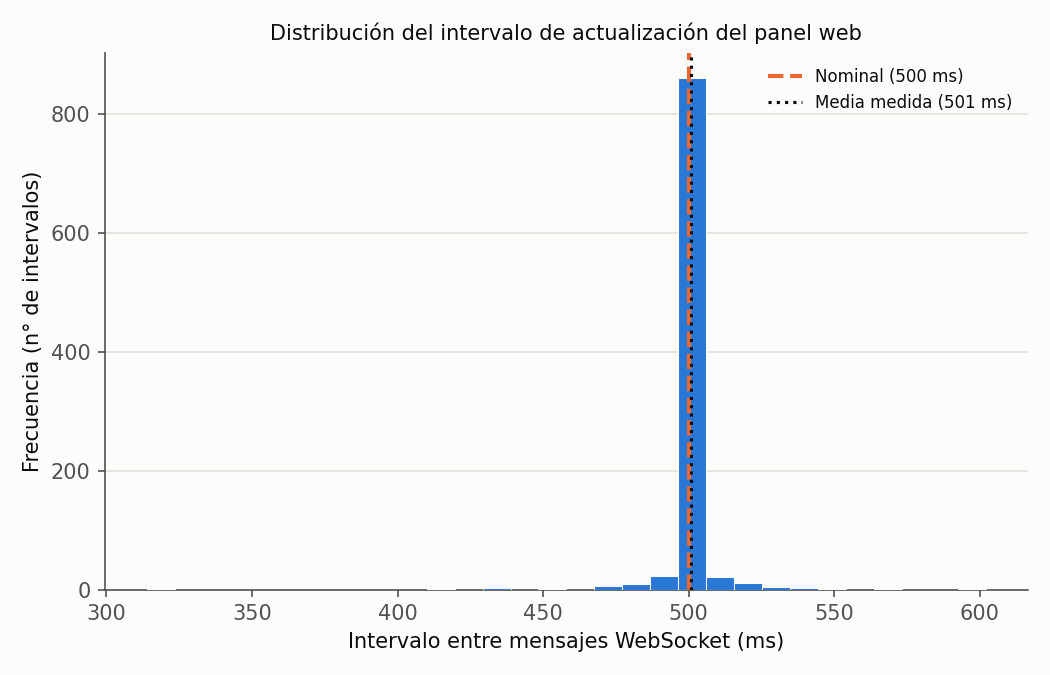
\includegraphics[width=0.8\textwidth]{Images/figura_ws_latencia.png}

	\vspace{2pt}
	{\footnotesize\textit{Nota.} Histograma de los intervalos individuales, con líneas verticales marcando el valor nominal (500\,ms) y la media medida. Se prefiere el histograma sobre otros tipos de gráfico porque la pregunta es ``qué tan dispersos están los intervalos alrededor del valor esperado'', una distribución de una sola variable continua. Elaboración propia.}
\end{figure}

\begin{table}[H]
	\centering
	\captionsetup{labelformat=simple, labelsep=newline, textfont=it, labelfont=bf, justification=raggedright, singlelinecheck=false}
	\caption{Estabilidad de la conexión WebSocket en sesión prolongada}
	\label{tab:estabilidad_ws}
	\begin{tabularx}{\textwidth}{X >{\centering\arraybackslash}p{3cm} >{\centering\arraybackslash}p{3.5cm}}
		\toprule
		\rowcolor[rgb]{0.851, 0.851, 0.851}
		Duración de la sesión & N.° de reconexiones & Observaciones \\
		\midrule
		8,1 min & 0 & Misma sesión de la Tabla~\ref{tab:latencia_panel}; sin caídas en todo el registro \\
		\bottomrule
	\end{tabularx}
	\vskip 0.15cm
	{\footnotesize \textit{Nota.} Reconexiones acumuladas reportadas por \texttt{wsStatsReport()} al cierre de la sesión. El reconector automático (\texttt{setTimeout(connectWs, 2000)}) hace que una caída puntual no requiera intervención manual; esta tabla registra cuántas veces ocurrió, no si el panel dejó de funcionar. La sesión registrada (8,1~min) es más corta que una sesión típica de uso, pero al no presentar ninguna reconexión aporta evidencia consistente con una conexión estable; ampliarla queda como posible verificación adicional.}
\end{table}

\begin{table}[H]
	\centering
	\captionsetup{labelformat=simple, labelsep=newline, textfont=it, labelfont=bf, justification=raggedright, singlelinecheck=false}
	\caption{Alcance del punto de acceso WiFi generado por el ESP32-S3}
	\label{tab:alcance_wifi}
	\begin{tabularx}{\textwidth}{>{\centering\arraybackslash}p{2.5cm} >{\centering\arraybackslash}p{3.5cm} >{\centering\arraybackslash}p{2.5cm} X}
		\toprule
		\rowcolor[rgb]{0.851, 0.851, 0.851}
		Distancia (m) & Obstáculos & ¿Conectado? & Reconectó al acercarse \\
		\midrule
		{}5 & Si (pared) & \checkmark & - \\
		{}10 & Si (pared) & \checkmark & - \\
		{}20 & Si (cuartos) & \checkmark & - \\
		\bottomrule
	\end{tabularx}
	\vskip 0.15cm
	{\footnotesize \textit{Nota.} Distancia aproximada entre el punto de acceso (ESP32-S3, dentro del vehículo) y el dispositivo que muestra el panel; agregar una fila por cada distancia probada.}
\end{table}

\subsection{Pruebas de consumo energético y modo de bajo consumo}
\label{sec:pruebas_consumo}

Esta prueba requiere medir corriente directamente sobre la placa (un multímetro o pinza en serie con la alimentación de 12\,V), algo que todavía no es posible con el prototipo actual sobre protoboard sin alterar el cableado de forma poco representativa. Queda pendiente hasta contar con la PCB ensamblada (Capítulo~5); mientras tanto, la Tabla~\ref{tab:consumo_energetico} ya incorpora la corriente \emph{teórica} de cada modo, derivada en la Sección~\ref{sec:consumo_activo} (modos activos) y la Ecuación~\eqref{eq:i12v_reposo} (\textit{deep sleep}) del Capítulo~3, y deja la columna de corriente medida en blanco para completarla en cuanto la PCB esté disponible.

\begin{table}[H]
	\centering
	\captionsetup{labelformat=simple, labelsep=newline, textfont=it, labelfont=bf, justification=raggedright, singlelinecheck=false}
	\caption{Consumo de corriente en los distintos modos de operación, teórico y medido}
	\label{tab:consumo_energetico}
	\begin{tabularx}{\textwidth}{X >{\centering\arraybackslash}p{4cm} >{\centering\arraybackslash}p{4cm}}
		\toprule
		\rowcolor[rgb]{0.851, 0.851, 0.851}
		Modo de operación & Corriente teórica (mA) & Corriente medida (mA) \\
		\midrule
		Activo, pantalla y WiFi encendidos & $\sim$52 & {}[COMPLETAR, pendiente de PCB] \\
		Activo, solo registro CAN/MicroSD & $\sim$34 & [COMPLETAR, pendiente de PCB] \\
		Deep sleep & $\sim$8 & [COMPLETAR, pendiente de PCB] \\
		\bottomrule
	\end{tabularx}
	\vspace{2mm}
	\\
	\begin{minipage}{\linewidth}
		\small
		\textit{Nota.} Corriente teórica calculada a la entrada de 12\,V (\texttt{OBD2}), sumando el aporte de cada componente a su riel nativo y convirtiendo a través de la eficiencia estimada del TPS54302 ($\sim$80\,\%), igual que en la Sección~\ref{sec:consumo} del Capítulo~3. Son estimaciones de orden de magnitud, no mediciones.
	\end{minipage}
\end{table}

\section{Resultados obtenidos}

\subsection{Resultados de la validación de la comunicación CAN}

Los resultados de la Tabla~\ref{tab:validacion_can}, obtenidos con las herramientas de la Sección~3.1, muestran una diferencia sistemática y no marginal entre ambos dispositivos en los tres indicadores medidos:

\begin{itemize}
	\item \textbf{Tramas recibidas.} El sistema propio registró 2\,936 respuestas válidas en la ventana de 5~minutos frente a 1\,712 del ELM327, un 71,5\,\% más de tramas procesadas en el mismo intervalo.
	\item \textbf{Tasa de error.} El sistema propio no presentó ninguna trama con error de bus (0 de 2\,936), mientras que el ELM327 registró 34 respuestas de error o \textit{NO DATA} sobre 1\,746 intentos clasificados, una tasa de error de $\approx 1{,}9\,\%$.
	\item \textbf{Latencia.} La latencia promedio del sistema propio (2,2~ms) fue del orden de 100 veces menor que la del ELM327 (231,4~ms).
\end{itemize}

Esta diferencia es atribuible a la arquitectura de cada dispositivo y no a una falla del ELM327: el sistema propio accede al controlador TWAI del ESP32-S3 de forma nativa, con la trama de respuesta disponible en la propia pila de firmware apenas el hardware la recibe del bus. El ELM327, en cambio, resuelve cada solicitud a través de una capa adicional de comandos AT en texto ASCII, que el propio adaptador debe traducir hacia y desde tramas CAN, y transporta el resultado por un enlace Bluetooth serie. Son dos fuentes adicionales de retardo y de posibles pérdidas de trama, ausentes en una implementación con acceso directo al controlador CAN.

Para la finalidad específica de este proyecto (adquirir parámetros del motor a alta frecuencia y con baja latencia para integrar el consumo instantáneo), el sistema desarrollado demuestra un desempeño de comunicación superior al de un adaptador comercial genérico como el ELM327, no en la precisión del cálculo de consumo en sí (que se evalúa por separado, contra el aforo real, en la Sección~\ref{sec:validacion_cuantitativa}), sino específicamente en la capa de adquisición de datos de la que depende esa precisión: una mayor tasa de muestreo efectiva y una latencia baja y estable reducen el error de integración temporal del consumo acumulado, y una tasa de error nula evita que datos corruptos o ausentes se propaguen al cálculo de \texttt{fuel\_calc.cpp}.

\subsection{Resultados de precisión del modelo Speed-Density}
\label{sec:resultados_speed_density}

La prueba estática (Sección~4.3.3) ya arrojó resultados concretos: antes de calibrar, el modelo subestimaba el caudal de aire en ralentí y 1500\,rpm ($-23{,}7\,\%$ y $-9{,}8\,\%$) y lo sobrestimaba a 2500 y 3500\,rpm ($+4{,}7\,\%$ y $+18{,}7\,\%$); tras calibrar la tabla VE con esos mismos datos, el error residual bajó a un rango de $-0{,}02\,\%$ a $+1{,}03\,\%$ (Figura~\ref{fig:post_calibracion}, Capítulo~3), una validación que, como se explicó ahí, es circular por construcción y no basta por sí sola. La Tabla~\ref{tab:validacion_dinamica} cierra ese punto con la prueba dinámica (Sección~\ref{sec:sd_prueba_dinamica}): métricas calculadas sobre una ruta real que nunca participó en la calibración.

\begin{table}[H]
	\centering
	\captionsetup{labelformat=simple, labelsep=newline, textfont=it, labelfont=bf, justification=raggedright, singlelinecheck=false}
	\caption{Métricas de validación dinámica del modelo Speed-Density (ruta real, Nissan Vanette)}
	\label{tab:validacion_dinamica}
	\begin{tabularx}{\textwidth}{X >{\centering\arraybackslash}p{2.2cm} >{\centering\arraybackslash}p{2.2cm} >{\centering\arraybackslash}p{2.2cm} >{\centering\arraybackslash}p{2.2cm}}
		\toprule
		\rowcolor[rgb]{0.851, 0.851, 0.851}
		n muestras & RMSE (g/s) & MAE (g/s) & MAPE (\%) & Pearson $r$ \\
		\midrule
		777 & 2,159 & 1,343 & 32,24 & 0,789 \\
		\bottomrule
	\end{tabularx}
	\vskip 0.15cm
	{\footnotesize \textit{Nota.} Calculado por \texttt{speed\_density\_drive\_validation.py} sobre el registro completo de \texttt{speed\_density\_drive\_log.csv} (777 muestras válidas), sin ningún dato compartido con la calibración de la Sección~4.3.3. $R^2=0{,}622$.}
\end{table}

\begin{figure}[H]
	\centering
	\caption{Distribución del error porcentual del modelo Speed-Density, ruta real (Nissan Vanette)}
	\label{fig:histograma_error_sd}
	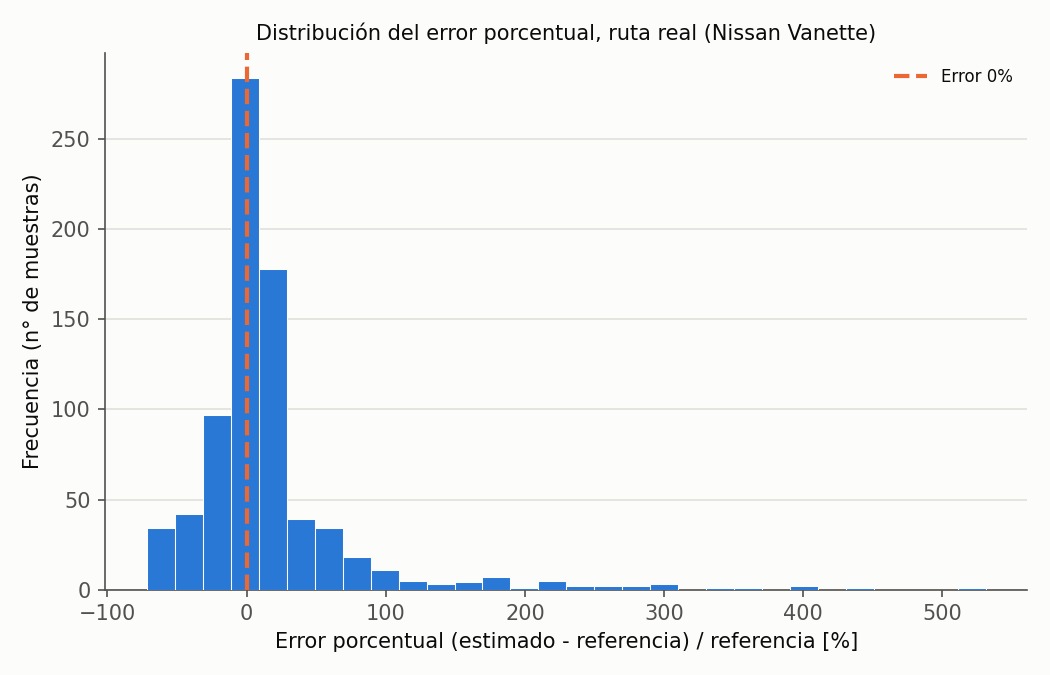
\includegraphics[width=0.8\textwidth]{Images/figura_histograma_error_dinamico.png}

	\vspace{2pt}
	{\footnotesize\textit{Nota.} Distribución del error porcentual muestra a muestra durante la ruta real; complementa la dispersión estimado-vs-referencia de la Figura~\ref{fig:dispersion_dinamica}. Elaboración propia.}
\end{figure}

La prueba dinámica confirma lo que la validación circular de la Figura~\ref{fig:post_calibracion} no podía garantizar: sobre 777 muestras de una ruta real, ajenas a la calibración, el modelo mantiene una correlación fuerte con la referencia ($r=0{,}789$, $R^2=0{,}622$) y un error absoluto moderado (RMSE $2{,}16$\,g/s, MAE $1{,}34$\,g/s sobre un rango de referencia de 2 a 16\,g/s), pero el MAPE ($32{,}2\,\%$) es considerablemente mayor que el $\pm 1\,\%$ observado en la calibración estática, la brecha esperable entre calibrar y generalizar. La Figura~\ref{fig:dispersion_dinamica} muestra por qué: la mayoría de los puntos se agrupan cerca de la recta 1:1, pero hay dispersión notable a caudal de referencia bajo (cerca de $2$\,g/s, correspondiente a ralentí y desaceleración), donde el estimado se dispara hasta $14$\,g/s en algunas muestras. El histograma de la Figura~\ref{fig:histograma_error_sd} confirma el mismo patrón: el grueso de las muestras cae cerca de $0\,\%$ de error, con una cola larga de errores porcentuales muy grandes que solo puede venir de esas condiciones de flujo bajo, donde dividir entre una referencia pequeña amplifica cualquier discrepancia absoluta modesta. Dos causas probables, no excluyentes entre sí: (1) el modelo asume un régimen cuasiestático (Sección~\ref{sec:speeddensity} del Capítulo~3), hipótesis que se degrada durante transitorios de aceleración/desaceleración reales, ausentes en la prueba estática por diseño; y (2) las cuatro lecturas de PID (RPM, MAP, IAT, MAF) se consultan de forma secuencial, no simultánea, así que en un transitorio rápido cada una corresponde a un instante ligeramente distinto. De ahí que el MAPE agregado deba leerse con cautela: está dominado por unas pocas muestras de bajo caudal, mientras que RMSE y MAE, menos sensibles a denominadores pequeños, son el indicador más representativo del error típico en conducción real.

\begin{table}[H]
	\centering
	\captionsetup{labelformat=simple, labelsep=newline, textfont=it, labelfont=bf, justification=raggedright, singlelinecheck=false}
	\caption{Validación del modelo Speed-Density en el Changan Honor}
	\label{tab:validacion_changan_sd}
	\begin{tabularx}{\textwidth}{>{\centering\arraybackslash}p{3cm} X}
		\toprule
		\rowcolor[rgb]{0.851, 0.851, 0.851}
		Vehículo & Validación disponible \\
		\midrule
		Changan Honor & No soporta el PID~0x10 (MAF), por lo que no existe una referencia directa de caudal de aire contra la cual calcular RMSE/MAE/MAPE, ni en la prueba estática ni en la dinámica (Sección~\ref{sec:ve-general} del Capítulo~3, ``Caso sin MAF''). Su exactitud se evalúa en cambio de forma indirecta, a nivel de consumo acumulado, en la Tabla~\ref{tab:comparacion_consumo_changan} (Sección~4.4.5) frente al aforo real de tanque lleno. \\
		\bottomrule
	\end{tabularx}
	\vskip 0.15cm
	{\footnotesize \textit{Nota.} A diferencia del Vanette, aquí no aplica ninguna de las métricas punto a punto de la Tabla~\ref{tab:validacion_dinamica} por ausencia de sensor de referencia, no por falta de la prueba.}
\end{table}

\subsection{Resultados de la validación del sensor MAP frente a la altitud}

Los resultados de la Tabla~\ref{tab:validacion_map_altitud} son favorables en ambos vehículos, pero no del mismo tipo de evidencia. El \textbf{Changan Honor} sí soporta el PID~0x33, así que su fila compara dos sensores reales de la propia ECU entre sí (MAP contra presión barométrica real) y da una diferencia de $0{,}0\,\%$ ($63{,}0$ frente a $63{,}0$\,kPa): una confirmación directa de que el sensor MAP reporta la presión atmosférica real de La Paz. El \textbf{Nissan Vanette}, en cambio, no soporta el PID~0x33, así que su \texttt{baro\_kpa} cae al respaldo del modelo ISA evaluado en \texttt{SITE\_ALTITUDE\_M} (Subsección~\ref{subsec:etav-altitud} del Capítulo~3); su diferencia de $-2{,}5\,\%$ ($63{,}0$ frente a $64{,}6$\,kPa) es entonces una comparación del MAP contra un \emph{modelo} de la atmósfera estándar, no contra un segundo sensor real: una validación más débil, aunque igualmente favorable. El valor ISA de $64{,}6$\,kPa es además consistente con la predicción teórica ya calculada en el Capítulo~3 ($P(3600)\approx 64{,}9$\,kPa, Ecuación~\eqref{eq:isa}), la pequeña diferencia atribuible a la altitud exacta configurada ($3640$ frente a $3600$\,m).

En ambos casos la diferencia es pequeña (menos de 2\,kPa). Esto descarta un sesgo de calibración de fábrica en el sensor MAP de cualquiera de los dos vehículos y confirma que el método speed-density parte, en ambos, de una lectura de presión correctamente calibrada para la altitud de operación, sin necesitar ningún factor de corrección adicional, como se justificó en el Capítulo~3.

\subsection{Resultados de las pruebas del panel web (WebSocket/HMI)}
\label{sec:resultados_panel_web}

Los resultados de las Tablas~\ref{tab:latencia_panel}--\ref{tab:alcance_wifi} (Changan Honor) confirman que el panel es apto para monitoreo en tiempo real: el intervalo de actualización promedió 500,0\,ms con una desviación de solo 10,0\,ms frente al periodo nominal configurado (\texttt{WS\_PUSH\_PERIOD\_MS}), sin ninguna reconexión en el registro de 8,1\,min, y sin pérdida de enlace hasta 20\,m de distancia con paredes de por medio, más que suficiente para el uso previsto, con el dispositivo dentro del mismo vehículo. Estos resultados son evidencia objetiva de la confiabilidad del panel y complementan, desde la capa de comunicación, la percepción subjetiva relevada en la encuesta de usabilidad de la Sección~\ref{sec:usabilidad_cualitativa}.

\subsection{Comparación de consumo estimado vs. consumo real}

Esta sección constituye el resultado central de la validación, ya que contrasta tres cantidades sobre nueve tramos de referencia (el corto y el medio, cada uno con 2 repeticiones completas: ida y vuelta por repetición, 4 tramos por categoría; y el largo una sola vez, sin ida/vuelta, Sección~\ref{sec:protocolo_tanque}): el consumo estimado por el sistema propio (medido de forma continua durante cada tramo), el consumo estimado por el adaptador ELM327 junto con la aplicación comercial (medido en una sesión separada e inmediatamente posterior sobre la misma ruta, por la limitación de conexión simultánea explicada en la Sección~\ref{sec:elm327_ref}), y el consumo real determinado por el método de aforo de tanque lleno a tanque lleno.

Repetir los trayectos corto y medio, y registrar ida y vuelta por separado en vez de como un solo tramo de ida-y-vuelta, no es solo para acumular más distancia: de ahí sale la \textbf{repetibilidad} del sistema propio (coeficiente de variación entre pasadas del mismo trayecto y del mismo sentido) de la Sección~\ref{sec:validacion_cuantitativa}, que de otro modo no tendría con qué calcularse; separar ida de vuelta además evita mezclar dos perfiles de tráfico/pendiente potencialmente distintos bajo un mismo número. El aforo real solo existe a nivel del \textbf{total combinado} de los nueve tramos (un único llenado de referencia cubre a todos, no se repitió por tramo, Sección~\ref{sec:protocolo_tanque}), así que la fila de ``Total'' es la única que se puede comparar directamente contra el aforo real; las filas individuales sirven para comparar el sistema propio contra el ELM327 tramo por tramo. Las Tablas~\ref{tab:comparacion_consumo_vanette} y~\ref{tab:comparacion_consumo_changan} (una por vehículo) y la Figura~\ref{fig:comparacion_consumo_grafico} presentan estos valores en forma descriptiva; el análisis estadístico formal (RMSE, MAPE, concordancia de Bland-Altman) se desarrolla por separado en la Sección~\ref{sec:validacion_cuantitativa}. Al interpretar la columna del ELM327 conviene tener presente que su comparación contra el sistema propio está sujeta a la variabilidad adicional de tratarse de una pasada distinta del mismo trayecto, y no de la misma sesión de manejo.

\begin{figure}[H]
	\centering
	\caption{Ejemplo del trayecto corto}
	\label{fig:ruta_corta}
	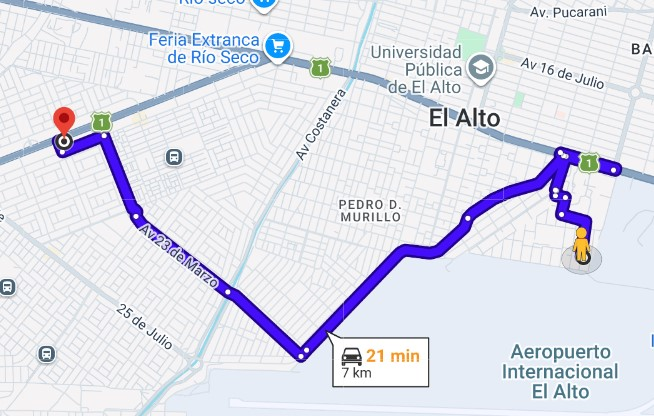
\includegraphics[width=0.8\textwidth]{Images/CORTO.jpg}
	\\
	\vspace{2pt}
	{\footnotesize\textit{Nota.} Recorrido de referencia del trayecto corto, con 2 repeticiones completas (ida y vuelta cada una, Tablas~\ref{tab:comparacion_consumo_vanette}/\ref{tab:comparacion_consumo_changan}); la ruta real puede variar levemente entre repeticiones. Elaboración propia.}
\end{figure}

\begin{figure}[H]
	\centering
	\caption{Ejemplo del trayecto medio}
	\label{fig:ruta_media}
	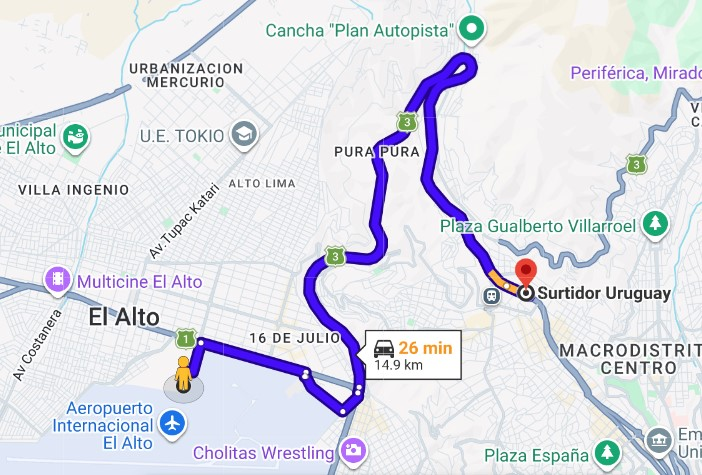
\includegraphics[width=0.8\textwidth]{Images/MEDIA.jpg}
	\\
	\vspace{2pt}
	{\footnotesize\textit{Nota.} Recorrido de referencia del trayecto medio, con 2 repeticiones completas (ida y vuelta cada una). Elaboración propia.}
\end{figure}

\begin{figure}[H]
	\centering
	\caption{Trayecto del viaje largo}
	\label{fig:ruta_larga}
	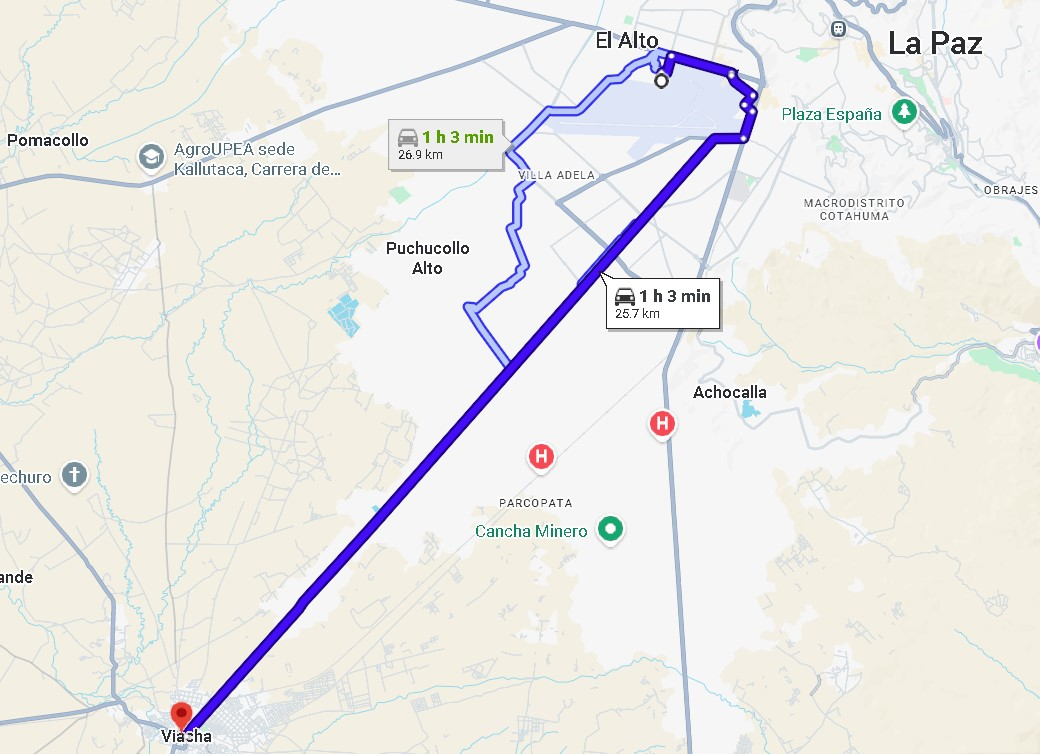
\includegraphics[width=0.8\textwidth]{Images/LARGO.jpg}
	\\
	\vspace{2pt}
	{\footnotesize\textit{Nota.} Recorrido único (sin repetición) del trayecto largo. Elaboración propia.}
\end{figure}

Las tres rutas de la Figura~\ref{fig:ruta_corta}--\ref{fig:ruta_larga} se recorrieron con \textbf{ambos vehículos} por separado, cada uno con su propio par de llenados de referencia; la Tabla~\ref{tab:comparacion_consumo_vanette} y la Tabla~\ref{tab:comparacion_consumo_changan} presentan los resultados de cada uno.

\begin{table}[H]
	\centering
	\captionsetup{labelformat=simple, labelsep=newline, textfont=it, labelfont=bf, justification=raggedright, singlelinecheck=false}
	\caption{Comparación de consumo de combustible entre el sistema propuesto, la referencia comercial y el consumo real, por trayecto (Nissan Vanette)}
	\label{tab:comparacion_consumo_vanette}
	\begin{tabularx}{\textwidth}{X >{\centering\arraybackslash}p{2.3cm} >{\centering\arraybackslash}p{2.8cm} >{\centering\arraybackslash}p{2.8cm} >{\centering\arraybackslash}p{2.8cm}}
		\toprule
		\rowcolor[rgb]{0.851, 0.851, 0.851}
		Trayecto & Distancia (km) & Sistema propuesto (L) & ELM327 + app (L)$^{a}$ & Real, tanque lleno (L) \\
		\midrule
		Viaje corto 1 (ida) & {}5,72 & 0,52 & 0,50 & --- \\
		Viaje corto 1 (vuelta) & 5,53 & 0,46 & 0,49 & --- \\
		Viaje corto 2 (ida) & 10,56 & 1,12 & 1,15 & --- \\
		Viaje corto 2 (vuelta) & 10,49 & 1,24 & 1,28 & --- \\
		Viaje medio 1 (ida) & 14,31 & 1,23 & 1,22 & --- \\
		Viaje medio 1 (vuelta) & 15,10 & 1,57 & 1,61 & --- \\
		Viaje medio 2 (ida) & 18,01 & 1,66 & 1,68 & --- \\
		Viaje medio 2 (vuelta) & 18,24 & 1,86 & 1,89 & --- \\
		Viaje largo & 26,3 & 2,43 & 2,44 & --- \\
		\midrule
		\textbf{Total (suma de los 9)} & \textbf{124,26} & \textbf{12,09} & \textbf{12,26} & \textbf{12,96} \\
		\bottomrule
	\end{tabularx}
	\vspace{2mm}
	\\
	\begin{minipage}{\linewidth}
		\small
		\textit{Nota.} Prototipo frente a herramienta comercial y reabastecimiento real. $^{a}$Sesión separada, misma ruta (Sección~\ref{sec:elm327_ref}). Aforo real solo en el total (Sección~\ref{sec:protocolo_tanque}). Viajes medio y largo: litros = gasto en Bs / 6,96\,Bs/L (\texttt{FUEL\_PRICE\_BS\_PER\_L}).
	\end{minipage}
\end{table}

\begin{table}[H]
	\centering
	\captionsetup{labelformat=simple, labelsep=newline, textfont=it, labelfont=bf, justification=raggedright, singlelinecheck=false}
	\caption{Comparación de consumo de combustible entre el sistema propuesto, la referencia comercial y el consumo real, por trayecto (Changan Honor)}
	\label{tab:comparacion_consumo_changan}
	\begin{tabularx}{\textwidth}{X >{\centering\arraybackslash}p{2.3cm} >{\centering\arraybackslash}p{2.8cm} >{\centering\arraybackslash}p{2.8cm} >{\centering\arraybackslash}p{2.8cm}}
		\toprule
		\rowcolor[rgb]{0.851, 0.851, 0.851}
		Trayecto & Distancia (km) & Sistema propuesto (L) & ELM327 + app (L)$^{a}$ & Real, tanque lleno (L) \\
		\midrule
		Viaje corto 1 (ida) & {}6,28 & 0,52 & 0,53 & --- \\
		Viaje corto 1 (vuelta) & 6,14 & 0.58 & 0,57 & --- \\
		Viaje corto 2 (ida) & 6,74 & 0,60 & 0,56 & --- \\
		Viaje corto 2 (vuelta) & 4.02 & 0,40 & 0,42 & --- \\
		Viaje medio 1 (ida) & 14,25 & 1,00 & 0,99 & --- \\
		Viaje medio 1 (vuelta) & 15,04 & 1,39 & 1,31 & --- \\
		Viaje medio 2 (ida) & 18,01 & 1,30 & 1,33 & --- \\
		Viaje medio 2 (vuelta) & 17,78 & 1,71 & 1,68 & --- \\
		Viaje largo & 25,99 & 1,839 & 1,825 & --- \\
		\midrule
		\textbf{Total (suma de los 9)} & \textbf{114,25} & \textbf{9,34} & \textbf{9,21} & \textbf{9,07} \\
		\bottomrule
	\end{tabularx}
	\vspace{2mm}
	\\
	\begin{minipage}{\linewidth}
		\small
		\textit{Nota.} Igual estructura que la Tabla~\ref{tab:comparacion_consumo_vanette}. Sin PID~0x10, ``sistema propuesto'' corre en Speed-Density puro; esta tabla es la validación aguas abajo de la Tabla~\ref{tab:validacion_changan_sd}. $^{a}$Ídem nota anterior.
	\end{minipage}
\end{table}

\begin{figure}[H]
	\centering
	\caption{Comparación gráfica del consumo de combustible por trayecto y vehículo según los tres métodos evaluados}
	\label{fig:comparacion_consumo_grafico}
	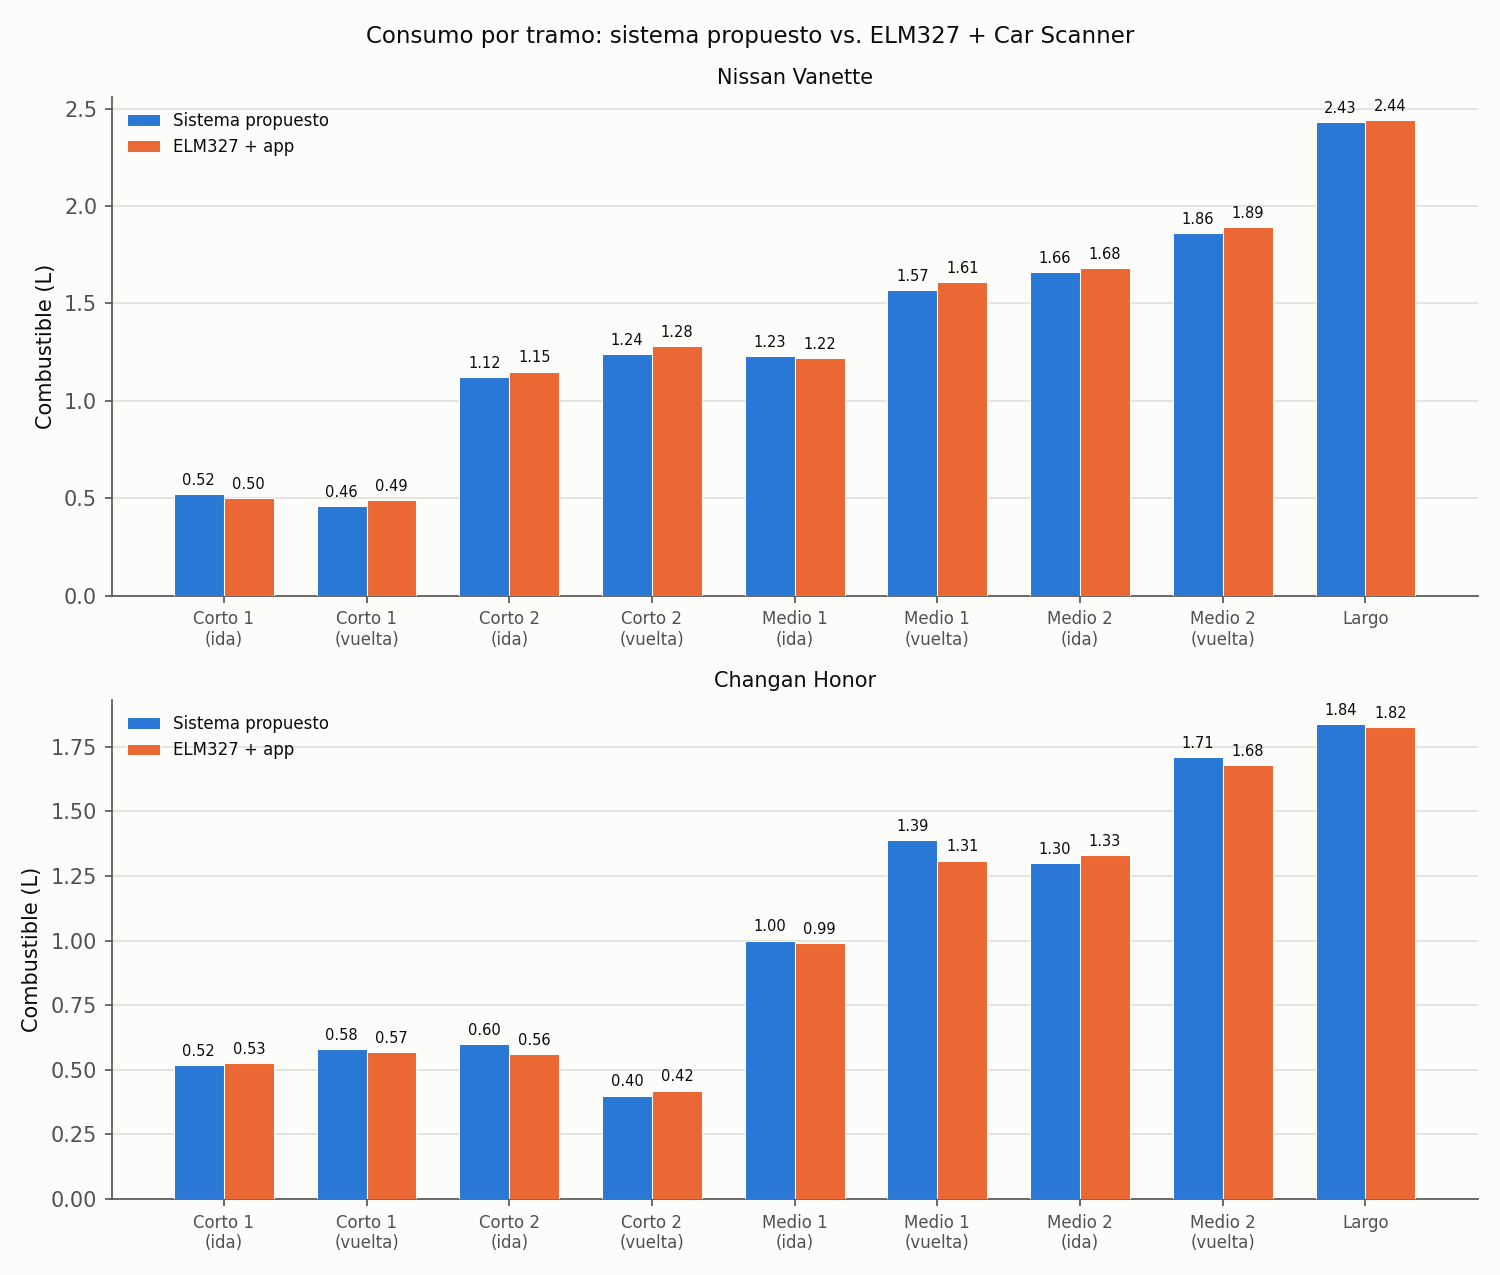
\includegraphics[width=\textwidth]{Images/figura_comparacion_consumo.png}

	\vspace{2pt}
	{\footnotesize\textit{Nota.} Comparativa del volumen de combustible estimado frente a las lecturas obtenidas por cada método, tramo por tramo, para cada vehículo. Elaboración propia.}
\end{figure}

Con los nueve tramos completos en ambos vehículos, el acuerdo entre el sistema propio y el ELM327 + Car Scanner vuelve a ser bueno en el total combinado ($-1{,}4\,\%$ en el Vanette: $12{,}090$ frente a $12{,}260$\,L en $124{,}26$\,km; y $+1{,}4\,\%$ en el Changan: $9{,}338$ frente a $9{,}212$\,L en $114{,}25$\,km), aunque, a diferencia de la comparación con solo tres trayectos, ahora el error por tramo individual oscila en ambos sentidos y con más dispersión: de $-6{,}1\,\%$ a $+4{,}0\,\%$ en el Vanette, y de $-4{,}8\,\%$ a $+7{,}1\,\%$ en el Changan, sin que el signo se mantenga constante ni siquiera entre ida y vuelta del mismo trayecto. Esto es consistente con lo ya discutido en la Figura~\ref{fig:ve_consumo_impacto}: el error por tramo depende de la mezcla de regímenes de motor de ese tramo en particular, no es una propiedad fija del ``trayecto corto'' o ``trayecto medio'' como categoría.

Al tener ahora dos repeticiones de cada categoría, se puede estimar por primera vez la \textbf{repetibilidad} del sistema propio (Sección~\ref{sec:validacion_cuantitativa}): el coeficiente de variación del consumo normalizado (L/100\,km) entre las 4 mediciones de cada categoría es de $13{,}6\,\%$ (corto) y $7{,}6\,\%$ (medio) en el Vanette, y de $6{,}9\,\%$ (corto) y $14{,}1\,\%$ (medio) en el Changan. Esta variabilidad, de un solo dígito alto a poco más de $13\,\%$, es del orden de magnitud esperable para conducción real en tráfico urbano de La Paz, donde el mismo trayecto nominal rara vez se recorre dos veces en condiciones idénticas (semáforos, tráfico, pendiente efectiva según el sentido); no debe leerse como ruido propio del sistema de medición, ya que la Tabla~\ref{tab:validacion_dinamica} ya mostró que el modelo, sobre las mismas condiciones de manejo, correlaciona fuertemente con el MAF real ($r=0{,}789$).

\subsubsection*{De dónde viene la diferencia: impacto de la curva VE en el consumo}

Las Tablas~\ref{tab:speed_density_resultados} y~\ref{tab:validacion_dinamica} ya mostraron que la tabla VE calibrada no es igual de precisa en todo el rango de régimen; lo que no muestran es cuánto vale eso en litros. La Figura~\ref{fig:ve_consumo_impacto}, generada por \texttt{CODIGOS/ve\_consumo\_impacto.py} sobre el mismo registro de la prueba dinámica (Sección~\ref{sec:sd_prueba_dinamica}), conecta ambas cosas: agrupa las muestras por bin de RPM y, en cada uno, calcula tanto el consumo instantáneo que resulta de la VE calibrada como el que resultaría del MAF real, expresando la diferencia directamente en L/100km en vez de en g/s de aire.

\begin{figure}[H]
	\centering
	\caption{Curva VE calibrada y su impacto en el consumo estimado, por bin de RPM (ruta real, Nissan Vanette)}
	\label{fig:ve_consumo_impacto}
	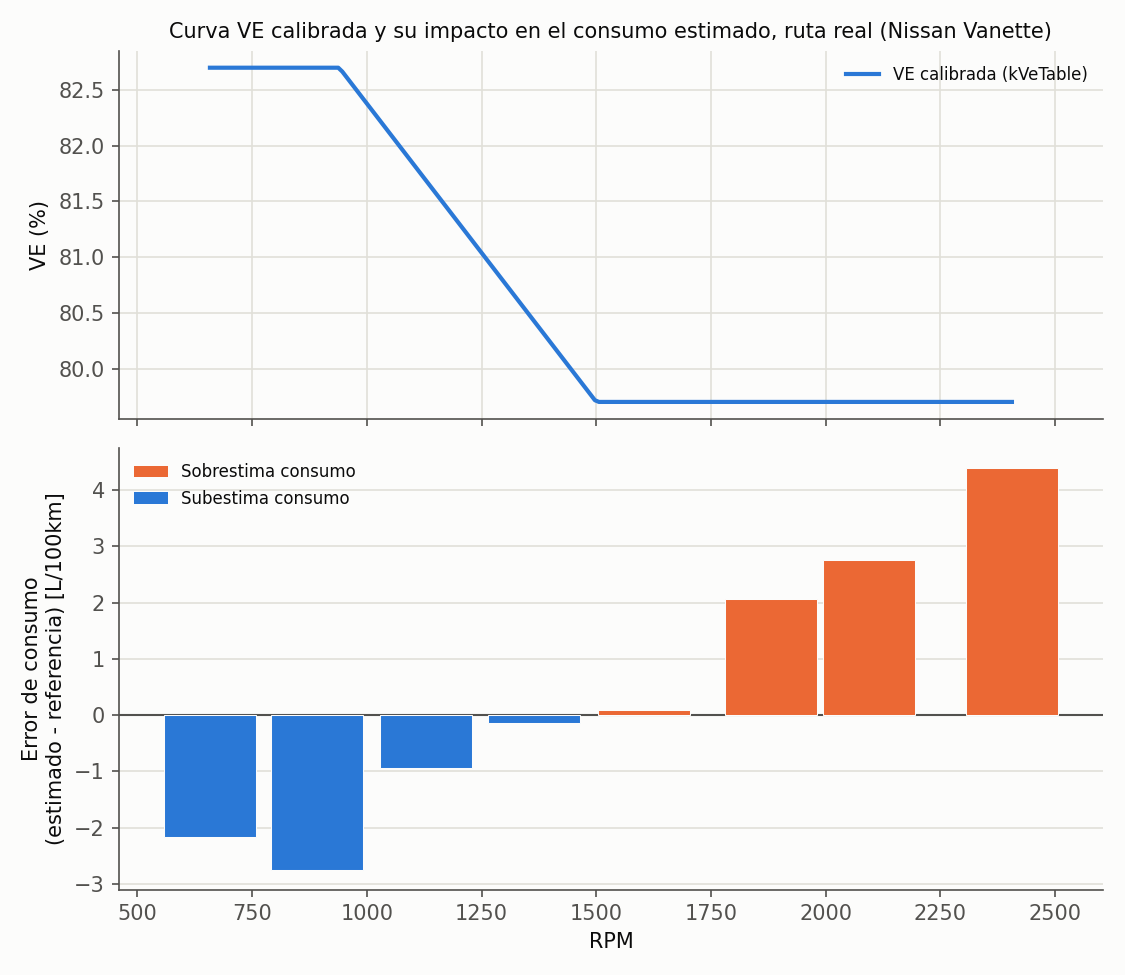
\includegraphics[width=0.85\textwidth]{Images/figura_ve_consumo_impacto.png}

	\vspace{2pt}
	{\footnotesize\textit{Nota.} Panel superior: curva VE calibrada (\texttt{kVeTable}) en el rango de RPM cubierto por la ruta. Panel inferior: error de consumo promedio por bin de RPM (estimado $-$ referencia), con barras coloreadas por signo. Ambos paneles comparten el eje de RPM para leer directamente en qué régimen se origina cada tramo de la diferencia. Elaboración propia.}
\end{figure}

El patrón es claro y consistente con la Figura~\ref{fig:histograma_error_sd}: por debajo de $\sim$1500\,rpm el sistema \textbf{subestima} el consumo (hasta $-2{,}7$\,L/100km en el bin de $\sim$890\,rpm), y por encima de $\sim$1600\,rpm lo \textbf{sobrestima}, con una brecha creciente que llega a $+4{,}4$\,L/100km cerca de $2400$\,rpm. Esto es consecuencia directa de la forma de la tabla VE calibrada (Tabla~\ref{tab:ve_calibracion}, Capítulo~3): con solo cuatro puntos calibrados contra régimen sostenido y sin datos por encima de $3500$\,rpm, la curva no captura del todo la variación real de la eficiencia volumétrica del motor durante los transitorios de una ruta: la misma limitación ya discutida en la Sección~\ref{sec:sd_prueba_dinamica}. En términos prácticos, esto explica por qué el error total de un trayecto del Vanette (Tabla~\ref{tab:comparacion_consumo_vanette}) no es simplemente la suma de errores aleatorios: depende de qué proporción del viaje se pasó en cada rango de régimen, de modo que una ruta con más tramos por encima de $1600$\,rpm tenderá a mostrar una sobrestimación neta mayor que una de manejo predominantemente urbano a bajas revoluciones.

\subsection{Desempeño del sistema en condiciones reales de conducción}

Con los nueve tramos ya medidos en ambos vehículos (Tablas~\ref{tab:comparacion_consumo_vanette} y~\ref{tab:comparacion_consumo_changan}), el sistema propio se mantiene cerca del ELM327 + Car Scanner en el total combinado: $-1{,}4\,\%$ en el Vanette, $+1{,}4\,\%$ en el Changan (Sección~\ref{sec:validacion_cuantitativa} desarrolla las métricas formales sobre estos mismos datos). Vale la pena notar la aparente contradicción con el $32\,\%$ de MAPE de la Sección~\ref{sec:resultados_speed_density}: esas cifras no son incompatibles, sino que miden cosas distintas. El MAPE se calcula muestra a muestra, así que un error grande y de signo variable en cada instante (Figura~\ref{fig:ve_consumo_impacto}) puede compensarse casi por completo al integrarlo en litros a lo largo de todo un trayecto, si el tiempo pasado sobrestimando y subestimando es comparable. En otras palabras: el modelo es menos preciso instante a instante de lo que sugiere el litraje total de un viaje, una distinción relevante para cualquier uso que dependa de la lectura instantánea (por ejemplo, retroalimentar el estilo de conducción en tiempo real) y no solo del acumulado al final del trayecto.

Los tramos cortos fueron viajes de no más de 15 minutos circulando en la ciudad de El Alto: el terreno fue en general plano, con la excepción del tráfico denso en los distintos puntos céntricos recorridos. Los tramos medios cubrieron mayor distancia y se realizaron por dos zonas distintas de la urbe paceña, cada una con su propia condición particular. Uno de ellos aprovechó la autopista La Paz-El Alto, donde se observa una asimetría clara entre ida y vuelta: en la bajada el acelerador no se pisa de forma continua, lo que se refleja en el menor consumo registrado por el sistema (Medio~1 ida, $8{,}60$\,L/100\,km, Tabla~\ref{tab:comparacion_consumo_vanette}); en la subida de vuelta, en cambio, el acelerador se mantiene pisado por más tiempo, y el consumo sube de forma correspondiente ($10{,}40$\,L/100\,km). El otro tramo medio se realizó por las avenidas principales de la ciudad de La Paz, esta vez con mayor peso a bordo del vehículo, factor que también influye en el consumo. En todos los tramos cortos y medios la temperatura ambiente fue fría, ya que las pruebas se realizaron de madrugada o por la noche.

En el viaje largo a Viacha, el sistema reaccionó de forma más lenta de lo esperado al inicio del trayecto, pero se estabilizó conforme avanzó el recorrido, resultado consistente con la calibración de la curva de eficiencia volumétrica del Nissan Vanette (Sección~\ref{sec:calibracion_speed_density}). Comparado con el Changan Honor, se esperaba, y se observó en el total combinado (Tablas~\ref{tab:comparacion_consumo_vanette}/\ref{tab:comparacion_consumo_changan}), un consumo menor en el Changan, coherente con su cilindrada más pequeña frente a la del Vanette.

\section{Validación del sistema}
\label{sec:validacion_cuantitativa}

\subsection{Validación cuantitativa (error porcentual y métricas estadísticas)}

Tomando como insumo los mismos trayectos ya presentados de forma descriptiva en las Tablas~\ref{tab:comparacion_consumo_vanette} y~\ref{tab:comparacion_consumo_changan} (Sección~4.4), se recomienda calcular, para cada conjunto de datos comparado (sistema propio frente a ELM327 y app, y sistema propio frente al consumo real de tanque lleno), las siguientes métricas (con las herramientas y fórmulas ya detalladas en la Sección~\ref{sec:herramientas_analisis}):

\begin{itemize}
	\item \textbf{Error porcentual relativo}, punto a punto, definido como:
	\begin{equation}
		\text{Error}_{\%} = \frac{|V_{\text{estimado}} - V_{\text{referencia}}|}{V_{\text{referencia}}} \times 100
		\label{eq:error_porcentual_relativo}
	\end{equation}
	\item \textbf{Error cuadrático medio (RMSE)} y \textbf{error absoluto medio (MAE)}, que expresan la magnitud típica del error en las mismas unidades que la variable medida (litros o litros por cada 100\,km), sobre los $n$ tramos comparados:
	\begin{equation}
		\text{RMSE} = \sqrt{\frac{1}{n}\sum_{i=1}^{n}\left(V_{\text{estimado},i} - V_{\text{referencia},i}\right)^2}
		\label{eq:rmse}
	\end{equation}
	\begin{equation}
		\text{MAE} = \frac{1}{n}\sum_{i=1}^{n}\left|V_{\text{estimado},i} - V_{\text{referencia},i}\right|
		\label{eq:mae}
	\end{equation}
	\item \textbf{Error porcentual absoluto medio (MAPE)}, útil para comparar el desempeño entre trayectos de distinta longitud; es el promedio del error porcentual relativo (Ecuación~\ref{eq:error_porcentual_relativo}) sobre los $n$ tramos:
	\begin{equation}
		\text{MAPE} = \frac{1}{n}\sum_{i=1}^{n}\frac{\left|V_{\text{estimado},i} - V_{\text{referencia},i}\right|}{V_{\text{referencia},i}} \times 100
		\label{eq:mape}
	\end{equation}
	\item \textbf{Coeficiente de correlación de Pearson} y \textbf{coeficiente de determinación ($R^2$)} de una regresión lineal entre los valores estimados y los de referencia, que indican qué tan bien se explica la variación de un método a partir del otro:
	\begin{equation}
		r = \frac{\displaystyle\sum_{i=1}^{n}\left(V_{\text{estimado},i}-\overline{V}_{\text{estimado}}\right)\left(V_{\text{referencia},i}-\overline{V}_{\text{referencia}}\right)}{\sqrt{\displaystyle\sum_{i=1}^{n}\left(V_{\text{estimado},i}-\overline{V}_{\text{estimado}}\right)^2}\ \sqrt{\displaystyle\sum_{i=1}^{n}\left(V_{\text{referencia},i}-\overline{V}_{\text{referencia}}\right)^2}}
		\label{eq:pearson_r}
	\end{equation}
	con $R^2 = r^2$ para el caso de una regresión lineal simple entre las dos series.
	\item \textbf{Análisis de concordancia de Bland-Altman}, recomendado específicamente para comparar dos métodos de medición que estiman una misma magnitud, como es el caso del sistema propuesto frente al adaptador ELM327 con su aplicación comercial. Este método grafica la diferencia entre ambas mediciones contra su promedio, y permite estimar el sesgo medio y los límites de concordancia, evidenciando si existe un sesgo sistemático entre los dos sistemas y no solo una correlación:
	\begin{align}
		d_i &= V_{\text{estimado},i} - V_{\text{referencia},i} \label{eq:ba_diferencia}\\
		\overline{d} &= \frac{1}{n}\sum_{i=1}^{n} d_i \qquad \text{(sesgo medio)} \label{eq:ba_sesgo}\\
		\text{LoA} &= \overline{d} \pm 1{,}96\, s_d \label{eq:ba_loa}
	\end{align}
	donde $s_d$ es la desviación estándar (muestral) de las diferencias $d_i$.
	\item \textbf{Repetibilidad}, expresada como el coeficiente de variación del sistema propio al repetir el mismo trayecto varias veces bajo condiciones similares; esto separa el error atribuible al método de estimación del error atribuible a la variabilidad de la conducción. Se calcula sobre las $n=4$ mediciones de consumo normalizado (L/100\,km) de una misma categoría de trayecto (ida y vuelta $\times$ 2 repeticiones) y vehículo:
	\begin{equation}
		\text{CV} = \frac{s}{\overline{x}} \times 100
		\label{eq:cv_repetibilidad}
	\end{equation}
	con $\overline{x}$ la media y $s$ la desviación estándar de esas $n=4$ mediciones.
\end{itemize}

La Tabla~\ref{tab:metricas_validacion} propone el formato de resumen de estas métricas.

\begin{table}[H]
	\centering
	\small
	\captionsetup{labelformat=simple, labelsep=newline, textfont=it, labelfont=bf, justification=raggedright, singlelinecheck=false}
	\caption{Resumen de métricas de validación cuantitativa}
	\label{tab:metricas_validacion}
	\begin{tabularx}{\textwidth}{X >{\centering\arraybackslash}p{3.2cm} >{\centering\arraybackslash}p{3.2cm}}
		\toprule
		\rowcolor[rgb]{0.851, 0.851, 0.851}
		Métrica & Sistema propio vs. ELM327+app & Sistema propio vs. tanque lleno \\
		\midrule
		RMSE (L) & 0,0312 & 0,64$^{c}$ \\
		MAE (L) & 0,0262 & 0,57$^{c}$ \\
		MAPE (\%) & 2,75 & 4,84$^{c}$ \\
		$R^2$ & 0,9971 & ---$^{c}$ \\
		Sesgo medio, Bland-Altman (L) & $-0,0024$ & ---$^{c}$ \\
		Límites de concordancia (L) & $[-0,0635,\ 0,0586]$ & ---$^{c}$ \\
		Repetibilidad$^{b}$ (CV, \%): Vanette corto & 13,6 & --- \\
		Repetibilidad$^{b}$ (CV, \%): Vanette medio & 7,6 & --- \\
		Repetibilidad$^{b}$ (CV, \%): Changan corto & 6,9 & --- \\
		Repetibilidad$^{b}$ (CV, \%): Changan medio & 14,1 & --- \\
		\bottomrule
	\end{tabularx}
	\vspace{2mm}
	\\
	\begin{minipage}{\linewidth}
		\small
		\textit{Nota.} Estadísticos de precisión, error global y concordancia evaluados para validar el ajuste numérico del modelo desarrollado frente a las referencias. Sistema propio vs. ELM327+app calculado sobre los 18 tramos combinados de ambos vehículos (Tablas~\ref{tab:comparacion_consumo_vanette}/\ref{tab:comparacion_consumo_changan}). $^{b}$La repetibilidad no es una comparación \textit{vs.}\ una referencia externa, sino la variabilidad del propio sistema (coeficiente de variación del consumo en L/100\,km) entre las 4 mediciones de cada categoría de trayecto por vehículo; se deja en la primera columna por consistencia visual con el resto de filas, y el guion en la segunda porque no aplica una comparación contra el tanque lleno. $^{c}$Sistema propio vs. tanque lleno tiene $n=2$ (el total del Vanette y el del Changan, Tablas~\ref{tab:comparacion_consumo_vanette}/\ref{tab:comparacion_consumo_changan}: único nivel en el que existe aforo real, Sección~\ref{sec:protocolo_tanque}); RMSE, MAE y MAPE se reportan igual sobre esos dos puntos, pero deben leerse como una referencia gruesa y no como una estimación estadísticamente robusta. $R^2$ y el análisis de Bland-Altman no se reportan en esta columna porque con $n=2$ el coeficiente de correlación es trivialmente $\pm 1$ (una recta pasa exactamente por cualquier par de puntos) y no refleja una bondad de ajuste real.
	\end{minipage}
\end{table}

\subsection{Validación cualitativa (usabilidad de la interfaz y confiabilidad)}
\label{sec:usabilidad_cualitativa}

Se recomienda complementar la validación numérica con una evaluación cualitativa breve de usabilidad, por ejemplo mediante una escala de Likert de 5 puntos aplicada a un pequeño grupo de usuarios (conductores de los vehículos de prueba o compañeros del programa), sobre aspectos como la claridad de la información mostrada en la pantalla OLED, la facilidad de acceso al panel web, y la percepción general de confiabilidad del dispositivo durante el uso cotidiano. Esta encuesta mide la \emph{percepción} del usuario; como contraparte objetiva de la afirmación ``confiaría en el valor mostrado'', la Sección~\ref{sec:resultados_panel_web} ya reporta datos medidos de la estabilidad y latencia reales de la conexión con el panel.

\begin{table}[H]
	\centering
	\captionsetup{labelformat=simple, labelsep=newline, textfont=it, labelfont=bf, justification=raggedright, singlelinecheck=false}
	\caption{Formato de encuesta de usabilidad (escala de Likert, 1 = muy en desacuerdo, 5 = muy de acuerdo)}
	\label{tab:usabilidad}
	\begin{tabularx}{\textwidth}{X *{5}{>{\centering\arraybackslash}p{1cm}}}
		\toprule
		\rowcolor[rgb]{0.851, 0.851, 0.851}
		Afirmación & 1 & 2 & 3 & 4 & 5 \\
		\midrule
		La información en la pantalla OLED es clara y legible & & &\checkmark & & \\
		El panel web es fácil de interpretar & & &\checkmark & & \\
		El dispositivo no interfiere con la conducción & & & & & \checkmark\\
		Confiaría en el valor de consumo mostrado & & & &\checkmark & \\
		\bottomrule
	\end{tabularx}
	\vspace{2mm}
	\\
	\begin{minipage}{\linewidth}
		\small
		\textit{Nota.} Cuestionario cualitativo diseñado para medir la percepción de usuario en aspectos de legibilidad, ergonomía e interfaz del prototipo desarrollado.
	\end{minipage}
\end{table}

\subsection{Discusión de resultados frente a los objetivos del proyecto}

Retomando los seis objetivos específicos planteados en el Capítulo~1, a continuación se discute, uno por uno, en qué medida los resultados de este capítulo los satisfacen:

\begin{itemize}
	\item \textbf{Determinar los parámetros del sistema OBD-II disponibles.} Se cumple: la Tabla~\ref{tab:pids_verificacion} confirma que ambos vehículos exponen RPM (\texttt{0x0C}) y velocidad (\texttt{0x0D}), pero difieren justo en el parámetro crítico del modelo: el Nissan Vanette reporta MAF (\texttt{0x10}) y el Changan Honor no. Esta asimetría, lejos de ser un obstáculo, es la que motivó desarrollar la ruta alternativa sin MAF (VE genérica y STFT/LTFT, Sección~\ref{sec:ve-general} del Capítulo~3) que exige implícitamente el objetivo al hablar de MAF \emph{y/o} MAP.

	\item \textbf{Desarrollar un modelo matemático de estimación basado en la relación aire-combustible.} Cumplido mediante el modelo Speed-Density calibrado en el Capítulo~3 y puesto a prueba en este: la calibración de la tabla VE con datos reales del Vanette (Sección~\ref{sec:calibracion_speed_density}) y su aplicación en la prueba dinámica de ruta real (Tabla~\ref{tab:validacion_dinamica}, $r=0{,}789$) muestran que el modelo captura la tendencia del caudal de aire real, aunque con una dispersión instantánea considerable (MAPE del $32\,\%$ punto a punto) que debe leerse como una limitación del modelo en sí, no solo de su calibración.

	\item \textbf{Adquirir y registrar datos del motor mediante OBD-II.} Este objetivo se cumple: el firmware adquiere y registra RPM, MAP o MAF, IAT y velocidad en cada ciclo, con una tasa de integridad de registro en MicroSD del $100\,\%$ (0 archivos corruptos en las tres sesiones de la Tabla~\ref{tab:validacion_microsd}, incluida una prueba deliberada de corte abrupto de energía).

	\item \textbf{Diseñar un sistema embebido de adquisición para validar el modelo.} Cumplido también: el prototipo basado en ESP32-S3 (Capítulo~3) fue el instrumento con el que se generaron todos los datos de este capítulo, desde la validación estática (Tabla~\ref{tab:speed_density_resultados}) hasta los nueve tramos de ruta real (Tablas~\ref{tab:comparacion_consumo_vanette}/\ref{tab:comparacion_consumo_changan}).

	\item \textbf{Diseñar e implementar una plataforma telemétrica IoT.} Cumplido de forma parcial. El ESP32-S3 sí actúa como servidor local, transmite la telemetría por WebSocket con latencia estable ($500{,}0 \pm 10{,}0$\,ms sobre 945 muestras, Tabla~\ref{tab:latencia_panel}) y sin reconexiones en la sesión prolongada registrada (Tabla~\ref{tab:estabilidad_ws}), y el punto de acceso WiFi se mantuvo conectado hasta los $20$\,m, la mayor distancia probada (Tabla~\ref{tab:alcance_wifi}), suficiente para el caso de uso dentro de un vehículo. Sin embargo, el objetivo específico planteaba explícitamente el almacenamiento en una \emph{base de datos estructurada}; lo efectivamente implementado es un registro en archivos CSV sobre MicroSD, sin una base de datos relacional o documental de por medio. Esta es una limitación real frente al objetivo original, que queda como trabajo futuro (por ejemplo, una capa de sincronización periódica del CSV hacia una base de datos en el servidor local o en la nube).

	\item \textbf{Evaluar el sistema integral bajo condiciones reales.} Cumplido con matices. El acuerdo global frente al ELM327 + Car Scanner es bueno sobre los nueve tramos ($-1{,}4\,\%$ Vanette, $+1{,}4\,\%$ Changan) y, frente al aforo real de tanque lleno, se mantiene en el mismo orden de magnitud (MAPE $\approx 4{,}8\,\%$, Sección~\ref{sec:validacion_cuantitativa}); pero dos limitaciones deben señalarse explícitamente. Primero, el tamaño de muestra es reducido —nueve tramos por vehículo y un único par de vehículos—, insuficiente para generalizar sin pruebas adicionales al resto de la flota de transporte público de La Paz. Segundo, los dos vehículos de prueba no se comportaron de forma equivalente frente al sistema: el Changan Honor, al no soportar el PID de MAF, solo pudo validarse de forma indirecta (a nivel de consumo acumulado) y no cuenta con la validación dinámica punto a punto que sí tiene el Vanette (Tabla~\ref{tab:validacion_dinamica}). Esta asimetría entre vehículos es en sí misma un hallazgo relevante, y amerita, como trabajo futuro, repetir la prueba dinámica en un vehículo adicional con sensor MAF para confirmar que el patrón de error observado no es específico de un solo motor.
\end{itemize}

Como cierre metodológico, conviene recordar que el modelo Speed-Density es, en sí mismo, una técnica ampliamente utilizada en unidades de control electrónico comerciales para la estimación del flujo de aire cuando no se dispone de un sensor MAF dedicado, y que su exactitud depende críticamente de una correcta caracterización de la eficiencia volumétrica del motor y de las condiciones ambientales; de ahí la pertinencia de las pruebas de corrección por altitud realizadas en este capítulo.
	% !TEX root = ../main.tex
% ============================================================================
% CAPÍTULO 5 — ANÁLISIS DE COSTOS Y PRESUPUESTO
% ============================================================================

\chapter{ANÁLISIS DE COSTOS Y PRESUPUESTO}

Este capítulo cuantifica el costo de desarrollar, fabricar y validar el sistema descrito en los Capítulos 3 y 4, y evalúa su viabilidad económica frente a alternativas comerciales existentes. El desglose sigue el mismo criterio de agrupación funcional ya establecido en la lista de materiales del Capítulo~3 (Tabla~\ref{bom}) y en la tabla de componentes del prototipo del Capítulo~4 (Tabla~\ref{tab:componentes_protoboard}). Así, cada partida de costo puede rastrearse hasta el componente físico concreto que la origina, en lugar de quedar como una cifra agregada sin respaldo.

Los montos se expresan en bolivianos (Bs), moneda de referencia ya utilizada en el resto de la tesis (por ejemplo, \texttt{FUEL\_PRICE\_BS\_PER\_L} en el firmware), con una columna equivalente en dólares (USD) para los componentes que se cotizan internacionalmente (LCSC, JLCPCB, AliExpress). Dado que el tipo de cambio BOB/USD ha tenido variaciones significativas en el mercado boliviano en los últimos años, las conversiones de este capítulo usan el tipo de cambio paralelo vigente al momento de la cotización, 11,60\,Bs/USD (agosto de 2026), y no un valor fijo asumido de antemano ni el tipo de cambio oficial, que en este periodo no refleja el costo real de acceso a dólares para la importación de componentes.

\section{Costos de componentes electrónicos}

Esta sección desglosa el costo de los componentes electrónicos en los mismos cuatro bloques funcionales de la Tabla~\ref{bom}: procesamiento, alimentación, interfaz CAN y periféricos. Las cantidades de cada fila provienen directamente de esa tabla; aquí solo se añaden el precio unitario y el subtotal por bloque.

\subsection{Costos del módulo de procesamiento (ESP32-S3)}

\begin{table}[H]
	\centering
	\captionsetup{labelformat=simple, labelsep=newline, textfont=it, labelfont=bf, justification=raggedright, singlelinecheck=false}
	\caption{Costo del módulo de procesamiento}
	\label{tab:costo_procesamiento}
	\begin{tabularx}{\textwidth}{X >{\centering\arraybackslash}p{1.6cm} >{\centering\arraybackslash}p{2.6cm} >{\centering\arraybackslash}p{2.6cm} >{\centering\arraybackslash}p{2.6cm}}
		\toprule
		\rowcolor[rgb]{0.851, 0.851, 0.851}
		Componente & Cant. & Precio unit. (USD) & Precio unit. (Bs) & Subtotal (Bs) \\
		\midrule
		Módulo ESP32-S3-WROOM-1-N16R8 (DevKitC-1, prototipo) & 1 & 9,48 & 110 & 110 \\
		\bottomrule
	\end{tabularx}
	\vspace{2mm}
	\\
	\begin{minipage}{\linewidth}
		\small
		\textit{Nota.} Precio de referencia del módulo de desarrollo completo (\textit{DevKitC-1}) usado en el prototipo sobre protoboard (Tabla~\ref{tab:componentes_protoboard}); si la versión final en PCB propia usa el módulo ESP32-S3-WROOM-1-N16R8 suelto en vez del DevKit completo, el precio unitario es menor pero requiere programador externo para el primer flasheo.
	\end{minipage}
\end{table}

\subsection{Costos de la etapa de alimentación (buck y LDOs)}

\begin{table}[H]
	\centering
	\captionsetup{labelformat=simple, labelsep=newline, textfont=it, labelfont=bf, justification=raggedright, singlelinecheck=false}
	\caption{Costo de la etapa de alimentación de dos rieles}
	\label{tab:costo_alimentacion}
	\begin{tabularx}{\textwidth}{X >{\centering\arraybackslash}p{1.6cm} >{\centering\arraybackslash}p{2.6cm} >{\centering\arraybackslash}p{2.6cm} >{\centering\arraybackslash}p{2.6cm}}
		\toprule
		\rowcolor[rgb]{0.851, 0.851, 0.851}
		Componente & Cant. & Precio unit. (USD) & Precio unit. (Bs) & Subtotal (Bs) \\
		\midrule
		Convertidor buck síncrono TPS54302DDCR & 1 & 0,2538 & 2,94 & 2,94 \\
		LDO AMS1117-3.3 (riel 1) & 1 & 0,2039 & 2,37 & 2,37 \\
		LDO AP2112K-3.3TRG1 (riel 2) & 1 & 0.2043 & 2,37 & 2,37 \\
		Diodo Schottky SS34 (protección polaridad) & 1 & 0,039 & 0,45 & 0,45 \\
		Fusible PTC reseteable 1812L150/33GR & 1 & 0,0575 & 0,67 & 0,67 \\
		Inductor de potencia 10~\textmu H & 1 & 1,3769 & 15,97 & 15,97 \\
		Condensadores y resistencias pasivas (Tabla~\ref{bom}) & 16 & 0,7323 & 8,49 & 135,91 \\
		\bottomrule
	\end{tabularx}
	\vspace{2mm}
	\\
	\begin{minipage}{\linewidth}
		\small
		\textit{Nota.} Los pasivos (condensadores, resistencias) se cotizan casi siempre por cinta/carrete completo aunque el diseño solo use unas pocas unidades; a cantidad de prototipo (1 placa), su costo unitario efectivo suele ser mayor que en producción en volumen. Es algo esperable, que debería diluirse si el proyecto escala a una serie de unidades, según se discute en la Subsección~\ref{sec:costo_beneficio}.
	\end{minipage}
\end{table}

\subsection{Costos de la interfaz CAN (transceptor y protección)}

\begin{table}[H]
	\centering
	\captionsetup{labelformat=simple, labelsep=newline, textfont=it, labelfont=bf, justification=raggedright, singlelinecheck=false}
	\caption{Costo de la interfaz de bus CAN}
	\label{tab:costo_can}
	\begin{tabularx}{\textwidth}{X >{\centering\arraybackslash}p{1.6cm} >{\centering\arraybackslash}p{2.6cm} >{\centering\arraybackslash}p{2.6cm} >{\centering\arraybackslash}p{2.6cm}}
		\toprule
		\rowcolor[rgb]{0.851, 0.851, 0.851}
		Componente & Cant. & Precio unit. (USD) & Precio unit. (Bs) & Subtotal (Bs) \\
		\midrule
		Transceptor CAN SN65HVD230 & 1 & 1,5216 & 17,65 & 17,65 \\
		Resistor control de pendiente (10~k$\Omega$) & 1 & 0,0912 & 1,06 & 1,06 \\
		Resistor de terminación 120~$\Omega$ (\textit{footprint} opcional, no poblado) & 0 & --- & --- & 0{,}00 \\
		Condensador de desacople & 1 & 0,4296 & 4,98 & 4,98 \\
		\bottomrule
	\end{tabularx}
	\vspace{2mm}
	\\
	\begin{minipage}{\linewidth}
		\small
		\textit{Nota.} El resistor de terminación no se puebla por defecto (Tabla~\ref{bom}, nota $^{a}$), ya que el dispositivo se conecta en derivación a un bus CAN que el vehículo ya termina; se incluye en la tabla únicamente para dejar registrado el criterio de costo cero de esa partida, no por omisión.
	\end{minipage}
\end{table}

\subsection{Costos de periféricos (MicroSD, OLED, conectores)}

\begin{table}[H]
	\centering
	\captionsetup{labelformat=simple, labelsep=newline, textfont=it, labelfont=bf, justification=raggedright, singlelinecheck=false}
	\caption{Costo de periféricos de almacenamiento, visualización y conexión}
	\label{tab:costo_perifericos}
	\begin{tabularx}{\textwidth}{X >{\centering\arraybackslash}p{1.6cm} >{\centering\arraybackslash}p{2.6cm} >{\centering\arraybackslash}p{2.6cm} >{\centering\arraybackslash}p{2.6cm}}
		\toprule
		\rowcolor[rgb]{0.851, 0.851, 0.851}
		Componente & Cant. & Precio unit. (USD) & Precio unit. (Bs) & Subtotal (Bs) \\
		\midrule
		Zócalo MicroSD (\textit{push-push}) & 1 & 0,1318 & 1,53 & 1,53 \\
		Tarjeta MicroSD (capacidad de referencia) & 1 & 3,2141 & 37,28 & 37,28 \\
		Pantalla OLED SSD1306 I\textsuperscript{2}C 0,96 & 1 & 2,686 & 31,16 & 31,16 \\
		Conector OBD-II tipo A con cable & 1 & 0,8 & 9,28 & 9,28 \\
		LEDs indicadores + resistencias limitadoras & 4 & 0,2120 & 2,46 & 9,84 \\
		Resistencias \textit{pull-up} SPI/I\textsuperscript{2}C (Tabla~\ref{bom}) & 6 & 0,0460 & 0,53 & 3,20 \\
		\bottomrule
	\end{tabularx}
	\vspace{2mm}
	\\
	\begin{minipage}{\linewidth}
		\small
		\textit{Nota.} La capacidad de la tarjeta MicroSD es más una decisión de autonomía de registro que de costo: dado el tamaño de fila estimado en el Capítulo~4 ($\approx$100 bytes/fila a 1 muestra/s), incluso una tarjeta de 8~GB excede ampliamente los requisitos de años de uso continuo, así que pagar por mayor capacidad no tiene sentido.
	\end{minipage}
\end{table}

\section{Costos de desarrollo y software}

El conjunto de herramientas de desarrollo empleado (Visual Studio Code, la extensión PlatformIO IDE, el \textit{framework} \texttt{arduino-esp32}, y el editor EasyEDA en su capa gratuita para el esquemático y la PCB) es de uso libre y sin costo de licenciamiento, criterio de selección ya justificado en la Sección de herramientas del Capítulo~3. El costo real de esta partida no está en licencias, entonces, sino en el tiempo de ingeniería invertido en el diseño de hardware, el firmware y la interfaz web.

\begin{table}[H]
	\centering
	\captionsetup{labelformat=simple, labelsep=newline, textfont=it, labelfont=bf, justification=raggedright, singlelinecheck=false}
	\caption{Costo estimado de horas de ingeniería por etapa de desarrollo}
	\label{tab:costo_horas}
	\begin{tabularx}{\textwidth}{X >{\centering\arraybackslash}p{2.6cm} >{\centering\arraybackslash}p{2.6cm} >{\centering\arraybackslash}p{2.6cm}}
		\toprule
		\rowcolor[rgb]{0.851, 0.851, 0.851}
		Etapa & Horas estimadas & Tarifa (Bs/h) & Subtotal (Bs) \\
		\midrule
		Diseño de esquemático y PCB & 8 & 0 & 0 \\
		Desarrollo de firmware (adquisición, cálculo, almacenamiento) & 28 & 0 & 0 \\
		Desarrollo del panel web (HMI) & 28 & 0 & 0 \\
		Pruebas, calibración y depuración & 120 & 0 & 0 \\
		\midrule
		\textbf{Total} & \textbf{184} & --- & \textbf{0} \\
		\bottomrule
	\end{tabularx}
	\vspace{2mm}
	\\
	\begin{minipage}{\linewidth}
		\small
		\textit{Nota.} Horas estimadas a partir de la dedicación real registrada por el autor ($\approx$4\,h/día): 2 días (PCB), 1 semana (firmware y panel web, 7 días cada uno) y 1 mes (calibración, 30 días). La tarifa se deja en 0\,Bs/h a propósito. Este capítulo lo permite porque el objetivo es el costo de materiales y fabricación, no el valor de mercado de las horas de un proyecto de grado; el total de 184\,h queda documentado como referencia de esfuerzo, no como partida monetaria del presupuesto.
	\end{minipage}
\end{table}

\section{Costos de fabricación y ensamblaje}

\subsection{Costos de la placa preliminar (Robokit)}
\label{sec:costo_pcb_preliminar}

La placa preliminar en EasyEDA descrita en la Sección~\ref{sec:placa_preliminar} (Capítulo~4) es, hasta el momento, la única placa de este proyecto efectivamente fabricada y ensamblada; por eso es la que se usa como \textbf{costo real del prototipo} en el presupuesto consolidado de este capítulo (Tabla~\ref{tab:presupuesto_total}). Se encargó localmente a Robokit (La Paz), lo que evita el envío internacional y la aduana que sí aplican a una fabricación en JLCPCB (Subsección~\ref{sec:costo_pcb_final}).

\begin{table}[H]
	\centering
	\captionsetup{labelformat=simple, labelsep=newline, textfont=it, labelfont=bf, justification=raggedright, singlelinecheck=false}
	\caption{Costo de fabricación de la placa preliminar en Robokit}
	\label{tab:costo_pcb_preliminar}
	\begin{tabularx}{\textwidth}{X >{\centering\arraybackslash}p{2cm} >{\centering\arraybackslash}p{2.6cm}}
		\toprule
		\rowcolor[rgb]{0.851, 0.851, 0.851}
		Concepto & Cantidad & Subtotal (Bs) \\
		\midrule
		Fabricación de PCB (Robokit, La Paz) & 1 & 150,00 \\
		Ensamblaje (soldadura manual, propia) & --- & 0,00 \\
		\midrule
		\textbf{Total} & --- & \textbf{150,00} \\
		\bottomrule
	\end{tabularx}
	\vspace{2mm}
	\\
	\begin{minipage}{\linewidth}
		\small
		\textit{Nota.} Cotización y fabricación locales (La Paz), sin envío internacional ni aduana. El ensamblaje fue realizado por el propio autor, por lo que no tiene costo monetario adicional, consistente con el criterio ya aplicado en la Tabla~\ref{tab:costo_horas} (tarifa de horas propias en 0\,Bs/h).
	\end{minipage}
\end{table}

La lista de materiales real de esta placa (16 referencias, exportada desde EasyEDA) muestra que su etapa de alimentación es una regulación lineal simple (7805 + transistor de paso TIP42C) y no la conversión conmutada de dos rieles de la Tabla~\ref{tab:costo_alimentacion} —esa etapa es específica de la placa final—; el módulo ESP32-S3, el transceptor CAN, la pantalla OLED y la tarjeta microSD son los mismos ya presupuestados en las Tablas~\ref{tab:costo_procesamiento}, \ref{tab:costo_can} y~\ref{tab:costo_perifericos}, reutilizados desde la etapa de protoboard y conectados a esta placa mediante los conectores de la Tabla~\ref{tab:costo_placa_preliminar_bom} en vez de cableado suelto. Los indicadores LED y sus resistencias limitadoras también coinciden con los ya contabilizados en la Tabla~\ref{tab:costo_perifericos}, por lo que no se repiten aquí.

\begin{table}[H]
	\centering
	\captionsetup{labelformat=simple, labelsep=newline, textfont=it, labelfont=bf, justification=raggedright, singlelinecheck=false}
	\caption{Componentes adicionales de la placa preliminar (etapa de alimentación y conectores)}
	\label{tab:costo_placa_preliminar_bom}
	\begin{tabularx}{\textwidth}{X >{\centering\arraybackslash}p{1.6cm} >{\centering\arraybackslash}p{2.2cm} >{\centering\arraybackslash}p{2.2cm} >{\centering\arraybackslash}p{2.2cm}}
		\toprule
		\rowcolor[rgb]{0.851, 0.851, 0.851}
		Componente & Cant. & Precio unit. (USD) & Precio unit. (Bs) & Subtotal (Bs) \\
		\midrule
		Regulador lineal 7805 (TO-252) & 1 & 0,0979 & 1,14 & 1,14 \\
		Transistor de paso TIP42C (TO-220) & 1 & 0,1777 & 2,06 & 2,06 \\
		Capacitor electrolítico 220\,\textmu F & 1 & 0,1400 & 1,62 & 1,62 \\
		Capacitor electrolítico 22\,\textmu F & 1 & 0,1200 & 1,39 & 1,39 \\
		Capacitor cerámico 100\,nF & 2 & 0,0200 & 0,23 & 0,46 \\
		Resistor THT 47\,$\Omega$ 1\,W & 1 & 0,0112 & 0,13 & 0,13 \\
		Conector de entrada de alimentación, 4~pines (WJ301V-5.0) & 1 & 0,1700 & 1,97 & 1,97 \\
		Header 4~pines (pantalla OLED) & 1 & 0,0198 & 0,23 & 0,23 \\
		Header 6~pines (transceptor SN65HVD230) & 1 & 0,0298 & 0,35 & 0,35 \\
		Header 8~pines (módulo microSD) & 1 & 0,0400 & 0,46 & 0,46 \\
		\midrule
		\textbf{Total} & --- & --- & --- & \textbf{9,81} \\
		\bottomrule
	\end{tabularx}
	\vspace{2mm}
	\\
	\begin{minipage}{\linewidth}
		\small
		\textit{Nota.} Precios de referencia LCSC para las referencias de fabricante exportadas desde EasyEDA (por ejemplo, \texttt{KS104M050C07RR0VH2FP0} para el capacitor de 100\,nF), convertidos a bolivianos al tipo de cambio de este capítulo (11,60\,Bs/USD); las referencias sin coincidencia exacta en el catálogo (capacitor de 22\,\textmu F, header de 8 pines y conector de 4 pines) se estiman por interpolación directa a partir de variantes de la misma familia con precio confirmado (por ejemplo, el conector WJ301V-5.0 sí tiene precio publicado en sus variantes de 2 y 3 pines), no por un valor arbitrario.
	\end{minipage}
\end{table}

\subsection{Costos de manufactura de la placa final (JLCPCB)}
\label{sec:costo_pcb_final}

A diferencia de la placa preliminar, la placa final documentada en el Capítulo~3 (diseñada en Altium Designer) todavía no se ha mandado a fabricar; esta subsección presenta su cotización de referencia, relevante si el proyecto avanza hacia esa versión más profesional o hacia una serie piloto para varios vehículos de transporte público. Se cotiza sobre el lote mínimo estándar de JLCPCB para placas de dos capas (Tabla~\ref{jlcpcb}, Capítulo~3), habitualmente de 5 unidades, que es también el tamaño de lote recomendado para tener margen ante fallas de soldadura o defectos de una unidad individual durante las pruebas iniciales.

\begin{table}[H]
	\centering
	\captionsetup{labelformat=simple, labelsep=newline, textfont=it, labelfont=bf, justification=raggedright, singlelinecheck=false}
	\caption{Costo de fabricación de PCB en JLCPCB}
	\label{tab:costo_pcb}
	\begin{tabularx}{\textwidth}{X >{\centering\arraybackslash}p{1.6cm} >{\centering\arraybackslash}p{2.2cm} >{\centering\arraybackslash}p{2.2cm} >{\centering\arraybackslash}p{2.2cm}}
		\toprule
		\rowcolor[rgb]{0.851, 0.851, 0.851}
		Concepto & Cantidad & Precio unit. (USD) & Precio unit. (Bs) & Subtotal (Bs) \\
		\midrule
		Fabricación de PCB (lote mínimo, 2 capas, 1~oz) & 1 & 4,00 & 46,40 & 46,40 \\
		Envío internacional (DHL/courier) & 1 & 38,00 & 440,80 & 440,80 \\
		Impuestos/aduana de importación (si aplica) & 1 & - & - & - \\
		\bottomrule
	\end{tabularx}
	\vspace{2mm}
	\\
	\begin{minipage}{\linewidth}
		\small
		\textit{Nota.} El envío y la aduana suelen pesar más en el costo total que la fabricación misma para lotes de prototipo pequeños importados a Bolivia; conviene cotizar ambos conceptos por separado y no asumir que están incluidos en el precio de fabricación publicado por JLCPCB.
	\end{minipage}
\end{table}

\subsection{Costos de ensamblaje SMD de la placa final}

Para la placa final, el ensamblaje de los componentes de montaje superficial puede resolverse por dos vías con una disyuntiva clara de costo contra riesgo: el servicio de ensamblaje (PCBA) del propio fabricante, o el soldado manual con estación de aire caliente/soldadora de precisión. La placa preliminar (Sección~\ref{sec:costo_pcb_preliminar}), en cambio, ya se ensambló manualmente por el propio autor, sin necesidad de esta disyuntiva.

\begin{table}[H]
	\centering
	\captionsetup{labelformat=simple, labelsep=newline, textfont=it, labelfont=bf, justification=raggedright, singlelinecheck=false}
	\caption{Comparación de estrategias de ensamblaje SMD}
	\label{tab:costo_ensamblaje}
	\begin{tabularx}{\textwidth}{>{\raggedright\arraybackslash}p{3.2cm} X X}
		\toprule
		\rowcolor[rgb]{0.851, 0.851, 0.851}
		Criterio & Ensamblaje PCBA (JLCPCB) & Soldadura manual \\
		\midrule
		Costo & 1\,440,60 Bs (124,19 USD; incluye \textit{setup} + componentes + mano de obra) & Solo costo de componentes; tiempo propio no facturado \\
		Riesgo técnico & Bajo: máquina \textit{pick-and-place} coloca el TPS54302DDCR (SOT-23-6) sin riesgo de puente de soldadura & Medio-alto en los pasivos 0603 y el regulador \textit{buck}, componentes de paso fino \\
		Tiempo de entrega & Sujeto al lote de fabricación + envío & Inmediato una vez recibida la PCB desnuda \\
		Recomendado cuando & Se fabrica más de una unidad, o no se dispone de estación de retrabajo SMD & Se ensambla una sola unidad de prototipo y ya se cuenta con el equipo de soldadura \\
		\bottomrule
	\end{tabularx}
	\vspace{2mm}
	\\
	\begin{minipage}{\linewidth}
		\small
		\textit{Nota.} Elaboración propia. Comparación de referencia para cuando se mande a fabricar la placa final; la vía efectivamente utilizada para la placa preliminar ya construida (Tabla~\ref{tab:costo_pcb_preliminar}) fue la soldadura manual (columna derecha), con el mismo criterio de costo cero de mano de obra propia que el resto del capítulo.
	\end{minipage}
\end{table}

\section{Costos de pruebas y validación}

\begin{table}[H]
	\centering
	\captionsetup{labelformat=simple, labelsep=newline, textfont=it, labelfont=bf, justification=raggedright, singlelinecheck=false}
	\caption{Costos asociados a la fase de pruebas y validación (Capítulo 4)}
	\label{tab:costo_pruebas}
	\begin{tabularx}{\textwidth}{X >{\centering\arraybackslash}p{2.6cm} >{\centering\arraybackslash}p{2.6cm} >{\centering\arraybackslash}p{2.6cm}}
		\toprule
		\rowcolor[rgb]{0.851, 0.851, 0.851}
		Concepto & Cantidad & Precio unit. (Bs) & Subtotal (Bs) \\
		\midrule
		Adaptador ELM327 Bluetooth (referencia de validación) & 1 & 85,00 & 85,00 \\
		Suscripción \textit{Car Scanner} Premium (3 meses) & 1 & 22,99 & 22,99 \\
		Combustible para trayectos de prueba tanque a tanque (Sección~\ref{sec:protocolo_tanque}, Cap.~4) & 22,03~L & 6,96 & 153,33 \\
		Instrumento de medición de corriente (tester) & 1 & 55,00 & 55,00 \\
		\midrule
		\textbf{Total} & --- & --- & \textbf{316,32} \\
		\bottomrule
	\end{tabularx}
	\vspace{2mm}
	\\
	\begin{minipage}{\linewidth}
		\small
		\textit{Nota.} El precio del litro de gasolina (6,96~Bs) es el mismo valor de referencia (\texttt{FUEL\_PRICE\_BS\_PER\_L}) que usa el propio firmware para calcular el costo acumulado del viaje (Capítulo~3), de modo que lo que reporta el dispositivo en campo y lo que presupuesta este capítulo quedan alineados. Los 22,03~L de combustible son la suma de los dos totales reales de aforo tanque lleno del Capítulo~4 (Nissan Vanette 12,96~L + Changan Honor 9,07~L, Tablas~\ref{tab:comparacion_consumo_vanette}/\ref{tab:comparacion_consumo_changan}): el consumo efectivamente gastado en los nueve tramos de prueba de ambos vehículos, no la capacidad de los tanques.
	\end{minipage}
\end{table}

\section{Presupuesto total del proyecto}

La Tabla~\ref{tab:presupuesto_total} consolida los subtotales de las secciones anteriores, usando la placa preliminar de Robokit (Sección~\ref{sec:costo_pcb_preliminar}) como fabricación real del prototipo. El presupuesto se presenta también en su forma de \textit{costo marginal por unidad adicional} (Tabla~\ref{tab:presupuesto_total}, última fila), escalando esta vez hacia la placa final en Altium Designer y su fabricación en JLCPCB (Sección~\ref{sec:costo_pcb_final}), relevante si el proyecto avanza hacia esa versión más profesional o hacia una pequeña serie de dispositivos para varios vehículos de transporte público, escenario directamente ligado a la motivación planteada en el Capítulo~1.

\begin{table}[H]
	\centering
	\captionsetup{labelformat=simple, labelsep=newline, textfont=it, labelfont=bf, justification=raggedright, singlelinecheck=false}
	\caption{Presupuesto total del proyecto, por categoría}
	\label{tab:presupuesto_total}
	\begin{tabularx}{\textwidth}{X >{\centering\arraybackslash}p{3.5cm} >{\centering\arraybackslash}p{3cm}}
		\toprule
		\rowcolor[rgb]{0.851, 0.851, 0.851}
		Categoría & Subtotal (Bs) & \%~del total \\
		\midrule
		Componentes electrónicos (Tablas~\ref{tab:costo_procesamiento}, \ref{tab:costo_can}, \ref{tab:costo_perifericos} y~\ref{tab:costo_placa_preliminar_bom}) & 235,79 & 33,58\,\% \\
		Desarrollo y software (Tabla~\ref{tab:costo_horas}) & 0,00 & 0,00\,\% \\
		Fabricación y ensamblaje, placa preliminar (Tabla~\ref{tab:costo_pcb_preliminar}) & 150,00 & 21,36\,\% \\
		Pruebas y validación (Tabla~\ref{tab:costo_pruebas}) & 316,32 & 45,05\,\% \\
		\midrule
		\textbf{Total del prototipo} & \textbf{702,11} & \textbf{100\,\%} \\
		\midrule
		Costo marginal estimado por unidad adicional, placa final$^{a}$ & 772,22 & --- \\
		\bottomrule
	\end{tabularx}
	\vspace{2mm}
	\\
	\begin{minipage}{\linewidth}
		\small
		\textit{Nota.} $^{a}$A diferencia del total del prototipo (que usa la placa preliminar de Robokit, ya fabricada), esta fila estima el costo de una unidad adicional producida por la vía de la placa final: excluye las horas de diseño de hardware/firmware (Tabla~\ref{tab:costo_horas}), que son un costo de desarrollo único (\textit{non-recurring engineering}) y no se repiten por unidad adicional fabricada. Incluye componentes (386,66\,Bs) más la fabricación de PCB y el ensamblaje PCBA a prorrata del lote mínimo de 5 unidades de JLCPCB (Tablas~\ref{tab:costo_pcb}/\ref{tab:costo_ensamblaje}: $(487{,}20+1\,440{,}60)/5 = 385{,}56$\,Bs), es decir $386{,}66+385{,}56=772{,}22$\,Bs por unidad adicional dentro del mismo lote.
	\end{minipage}
\end{table}

\begin{figure}[H]
	\centering
	\caption{Distribución porcentual del presupuesto total del proyecto por categoría}
	\label{fig:pastel_presupuesto}
	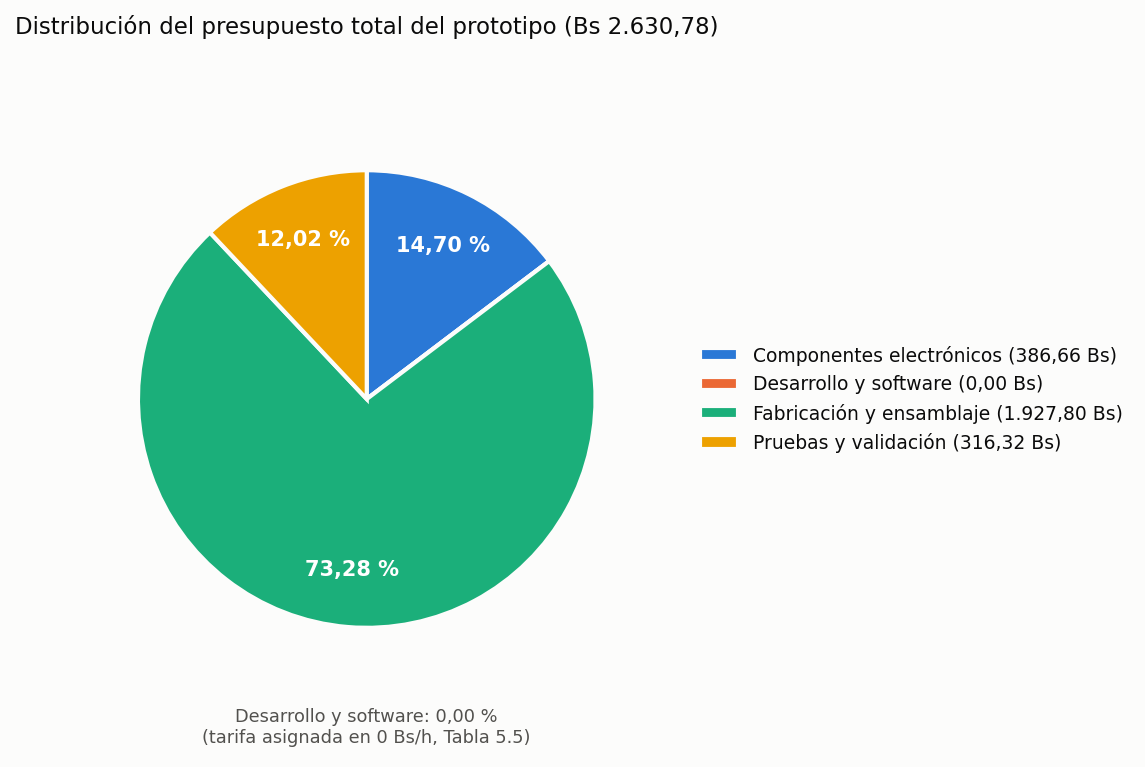
\includegraphics[width=0.85\textwidth]{Images/figura_presupuesto_pastel.png}

	\vspace{2pt}
	{\footnotesize\textit{Nota.} Se elige un gráfico de pastel porque las cuatro categorías son mutuamente excluyentes y suman el 100\,\% de un mismo presupuesto total; este tipo de gráfico comunica de forma directa qué proporción del gasto corresponde a componentes frente a mano de obra de desarrollo; una tabla de números no se lee con la misma claridad de un vistazo. Elaboración propia a partir de \texttt{CODIGOS/presupuesto\_pie.py} \citep{CalleGitHub2026}.}
\end{figure}

\section{Análisis de viabilidad económica}

\subsection{Comparación con soluciones comerciales existentes}

El sistema propuesto se contrasta contra dos categorías de alternativas ya mencionadas en los Antecedentes del Capítulo~1: los adaptadores OBD-II genéricos de bajo costo combinados con una aplicación móvil (por ejemplo, ELM327 + \textit{Car Scanner}, ya usado como referencia de validación en el Capítulo~4), y las plataformas de telemetría de flota comerciales orientadas a empresas de transporte.

\begin{table}[H]
	\centering
	\captionsetup{labelformat=simple, labelsep=newline, textfont=it, labelfont=bf, justification=raggedright, singlelinecheck=false}
	\caption{Comparación funcional y de costo frente a alternativas comerciales}
	\label{tab:comparacion_comercial}
	\begin{tabularx}{\textwidth}{>{\raggedright\arraybackslash}p{3.4cm} X X X}
		\toprule
		\rowcolor[rgb]{0.851, 0.851, 0.851}
		Criterio & Sistema propuesto & ELM327 + app comercial & Telemetría de flota comercial \\
		\midrule
		Costo inicial & 772,22 Bs$^{a}$ (Tabla~\ref{tab:presupuesto_total}) & 85,00 Bs (Tabla~\ref{tab:costo_pruebas}) & Desde 58\,000 Bs$^{b}$ (USD 5\,000, \textit{FuelForce}, pago único); el resto de proveedores cobra el hardware por separado, sin monto público \\
		Costo recurrente & Ninguno (sin suscripción) & Suscripción \textit{Car Scanner} Premium: 22,99\,Bs cada 3 meses & USD 4 a 100 por vehículo/mes según proveedor$^{b}$ ($\approx$46 a 1\,160\,Bs/mes) \\
		Registro local sin conexión a internet & Sí (microSD) & Depende de la app & Generalmente requiere conectividad \\
		Panel propio, sin dependencia de un tercero & Sí (SoftAP local) & No (depende del proveedor de la app) & No (plataforma del proveedor) \\
		Código y diseño abiertos, personalizables & Sí & No & No \\
		Corrección/\allowbreak calibración específica del vehículo & Sí (\texttt{FUEL\_\allowbreak CALIBRATION\_\allowbreak FACTOR}, tabla VE) & Limitada o inexistente & Variable según proveedor \\
		\bottomrule
	\end{tabularx}
	\vspace{2mm}
	\\
	\begin{minipage}{\linewidth}
		\small
		\textit{Nota.} Elaboración propia. $^{a}$Se usa el costo marginal por unidad adicional escalando a la placa final (Tabla~\ref{tab:presupuesto_total}) y no el presupuesto total del prototipo (702,11\,Bs, fabricado con la placa preliminar de Robokit), porque este segundo aún incluye los instrumentos de prueba del Capítulo~4 (ELM327, tester, combustible de validación) —costos de validación, no de una unidad desplegable—, mientras que la cifra de la placa final sí representa lo que costaría producir una unidad adicional a mayor escala, con un acabado más cercano al de un producto terminado y comparable con las alternativas comerciales de esta tabla. $^{b}$Precios de mercado internacional (no existe cotización pública para el mercado boliviano), tomados de \textit{Fleetio}, ``6 Best Fuel Monitoring Systems: 2025 Comparison Guide'' (\texttt{fleetio.com/blog/fuel-monitoring-systems}, consultado en agosto de 2026): Fleetio USD 4--10/vehículo/mes; Motive desde USD~25/vehículo/mes más costo de dispositivos ELD; Samsara USD 27--33/vehículo/mes (software; hardware facturado aparte); Geotab USD 35--100/vehículo/mes (software; hardware facturado aparte); FuelForce desde USD~5\,000 en modalidad de pago único por funcionalidad, en vez de suscripción. La conversión a bolivianos usa el mismo tipo de cambio de este capítulo (11,60\,Bs/USD).
	\end{minipage}
\end{table}

\begin{figure}[H]
	\centering
	\caption{Comparación de costo inicial entre el sistema propuesto y alternativas comerciales}
	\label{fig:barras_comparacion_comercial}
	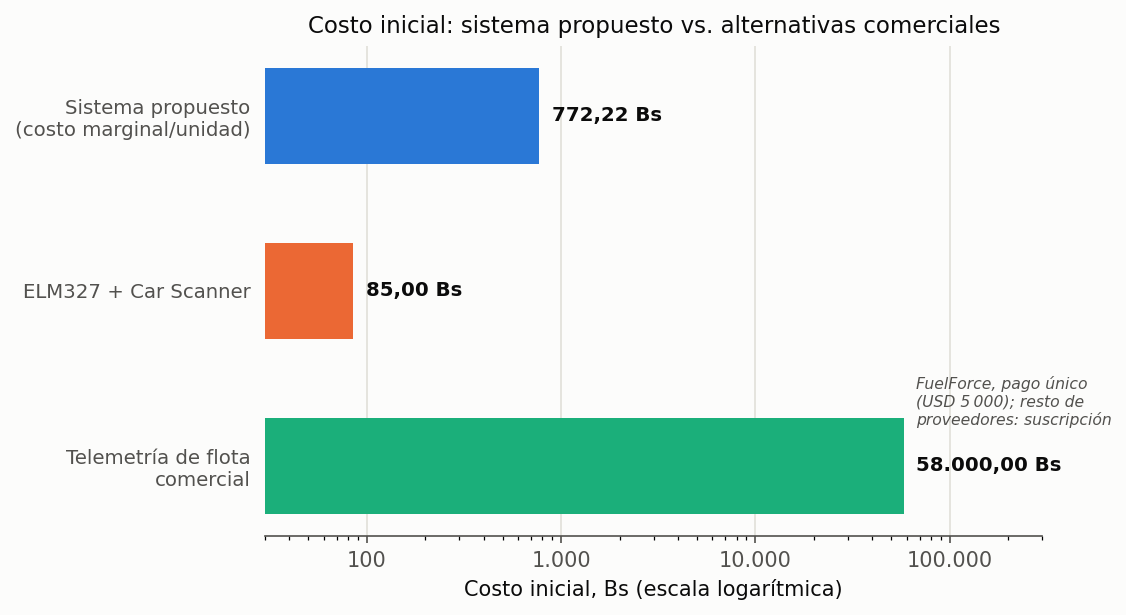
\includegraphics[width=0.85\textwidth]{Images/figura_comparacion_comercial.png}

	\vspace{2pt}
	{\footnotesize\textit{Nota.} Se elige un gráfico de barras horizontales, en vez de uno vertical, porque los nombres de las tres alternativas comparadas son largos y se leen mejor como etiquetas de eje horizontal; al ser solo tres categorías discretas comparadas por una única magnitud (costo), la barra es más directa de leer que un gráfico de líneas o de dispersión. El eje de costo usa escala logarítmica porque los tres valores abarcan casi tres órdenes de magnitud (85 a 58\,000\,Bs); cada barra conserva su valor exacto como etiqueta directa para que la escala no distorsione la lectura del monto real. El valor de telemetría de flota corresponde a un único proveedor (\textit{FuelForce}, pago único; Tabla~\ref{tab:comparacion_comercial}) y no a un promedio del rubro, ya que el resto de proveedores citados cobra por suscripción con hardware facturado aparte. Elaboración propia.}
\end{figure}

\subsection{Análisis costo-beneficio}
\label{sec:costo_beneficio}

El beneficio económico del sistema no proviene de evitar un gasto de compra (como en la comparación anterior), sino de la reducción de consumo de combustible que su uso puede inducir en el conductor al hacer visible, en tiempo real, un comportamiento de manejo ineficiente. El mecanismo exacto por el que un sistema de monitoreo reduce el consumo es de naturaleza conductual (retroalimentación al conductor) y no una modificación mecánica del vehículo, así que su magnitud solo puede estimarse una vez completada la comparación de consumo del Capítulo~4 (Tablas~\ref{tab:comparacion_consumo_vanette} y~\ref{tab:comparacion_consumo_changan}) entre trayectos con y sin atención activa al panel del dispositivo.

El periodo de recuperación de la inversión (\textit{payback period}) se estima como:

\begin{equation}
	T_{recuperación}\,[\text{meses}] = \frac{\text{Costo total del prototipo (Tabla~\ref{tab:presupuesto_total})}}{\text{Ahorro mensual estimado}\,[\text{Bs/mes}]}
	\label{eq:payback}
\end{equation}

donde el ahorro mensual se obtiene de multiplicar la reducción porcentual de consumo por retroalimentación al conductor (valor de literatura, ya que no se midió en este proyecto) por el gasto mensual de combustible típico del vehículo evaluado, a su vez estimado a partir del kilometraje mensual habitual (también de literatura) y el consumo promedio real observado en el Capítulo~4 (totales de aforo de las Tablas~\ref{tab:comparacion_consumo_vanette}/\ref{tab:comparacion_consumo_changan}).

\begin{table}[H]
	\centering
	\captionsetup{labelformat=simple, labelsep=newline, textfont=it, labelfont=bf, justification=raggedright, singlelinecheck=false}
	\caption{Estimación del periodo de recuperación de la inversión}
	\label{tab:payback}
	\begin{tabularx}{\textwidth}{X >{\centering\arraybackslash}p{3.5cm} >{\centering\arraybackslash}p{3.5cm}}
		\toprule
		\rowcolor[rgb]{0.851, 0.851, 0.851}
		Variable & Changan Honor & Nissan Vanette \\
		\midrule
		Kilometraje mensual estimado (km)$^{a}$ & 6\,000 & 6\,000 \\
		Consumo promedio (L/100\,km, Cap.~4)$^{b}$ & 7,94 & 10,43 \\
		Gasto mensual de combustible (Bs) & 3\,315,74 & 4\,355,57 \\
		Reducción de consumo atribuible al monitoreo (\%)$^{c}$ & 6,6 & 6,6 \\
		Ahorro mensual estimado (Bs/mes) & 218,84 & 287,47 \\
		Periodo de recuperación (meses) & 3,21 & 2,44 \\
		\bottomrule
	\end{tabularx}
	\vspace{2mm}
	\\
	\begin{minipage}{\linewidth}
		\small
		\textit{Nota.} $^{a}$No se midió el kilometraje real de estos vehículos: se usa un valor representativo (200\,km/día $\times$ 30 días) dentro del rango de 150 a 300\,km/día que reporta la literatura de operación de buses urbanos en servicio de todo el día \citep{PPIAF_UrbanBusToolkit_kpvpd}, igual para ambos vehículos al no existir un dato diferenciado por unidad. $^{b}$Consumo real de referencia (tanque lleno, no la estimación del sistema propio): total de aforo entre distancia total recorrida en los nueve tramos de prueba (Tablas~\ref{tab:comparacion_consumo_vanette}/\ref{tab:comparacion_consumo_changan}, Capítulo~4): Nissan Vanette $12{,}96/124{,}26\times100$; Changan Honor $9{,}07/114{,}25\times100$. $^{c}$La fila de reducción de consumo es la variable crítica de esta tabla y no se midió en este proyecto (requeriría un diseño experimental adicional al del Capítulo~4, por ejemplo contrastar el mismo trayecto con el panel visible frente al panel oculto para el conductor); se usa en su lugar el efecto promedio reportado por un metaanálisis de 17 estudios sobre sistemas de retroalimentación \textit{eco-driving} a bordo, $6{,}6\,\%$ de mejora en economía de combustible \citep{Sanguinetti2020EcoDriving}, dejando explícito que es un valor de literatura y no una medición propia.
	\end{minipage}
\end{table}

\begin{figure}[H]
	\centering
	\caption{Punto de equilibrio (\textit{breakeven}) entre el costo del dispositivo y el ahorro acumulado de combustible}
	\label{fig:breakeven}
	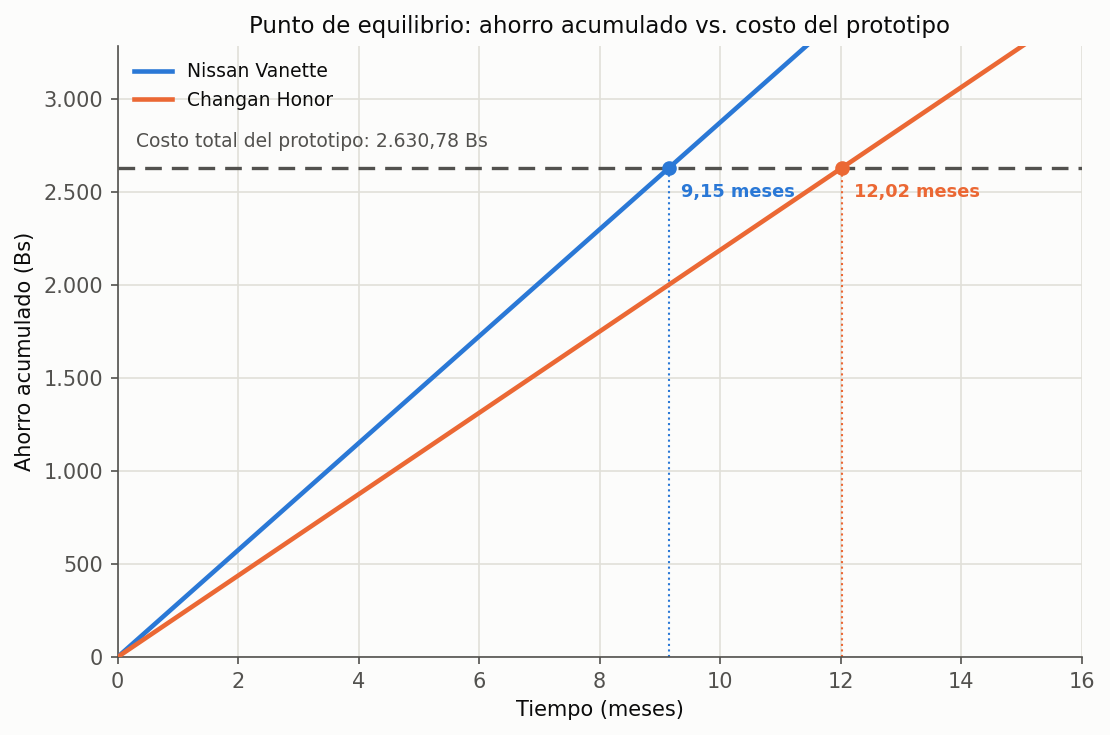
\includegraphics[width=0.85\textwidth]{Images/figura_breakeven.png}

	\vspace{2pt}
	{\footnotesize\textit{Nota.} Se elige un gráfico de líneas porque ambas magnitudes (costo fijo y ahorro acumulado) son funciones continuas del tiempo, y lo relevante para el lector es identificar visualmente el punto de cruce entre ambas curvas, algo que una tabla de valores puntuales no comunica con la misma inmediatez. Las rectas de ahorro acumulado y los periodos de recuperación (2,44 y 3,21 meses) se derivan del costo real del prototipo con la placa preliminar (Tabla~\ref{tab:presupuesto_total}) y de los valores de literatura de la Tabla~\ref{tab:payback} (kilometraje mensual y reducción de consumo atribuible al monitoreo); estos últimos no son una medición directa y el resultado debe leerse como una estimación, no como una garantía de recuperación en ese plazo exacto. Elaboración propia.}
\end{figure}

La viabilidad económica de este proyecto, para cerrar el capítulo, no depende únicamente de recuperar el costo de un prototipo individual: depende de su potencial de escalar a una pequeña serie de unidades para el transporte público de La Paz. En ese escenario, el costo marginal por unidad (Tabla~\ref{tab:presupuesto_total}), ya sin las horas de diseño amortizadas por este primer desarrollo, es la cifra económicamente relevante, y no el presupuesto total del prototipo aquí calculado.

	% !TEX root = ../main.tex
% ============================================================================
% CAPÍTULO 6 — CONCLUSIONES Y RECOMENDACIONES
% ============================================================================

\chapter{CONCLUSIONES Y RECOMENDACIONES}

\section{Conclusiones}

\subsection{Conclusiones respecto a los objetivos planteados}

A continuación se retoma cada objetivo específico del Capítulo~1 y se concluye sobre su grado de cumplimiento a partir de la evidencia de diseño (Capítulo~3) y de las pruebas experimentales (Capítulo~4).

\begin{itemize}
	\item \textbf{Determinación de los parámetros OBD-II disponibles.} El escaneo de PIDs realizado en campo sobre ambos vehículos de prueba (Sección~\ref{subsec:soporte_pids}, Capítulo~3) determinó de forma directa, no supuesta, que el Changan Honor no soporta el PID~0x10 (MAF) mientras que el Nissan Vanette sí; este hallazgo, además, fue el que justificó adoptar el método Speed-Density como vía principal de estimación. Objetivo cumplido.
	\item \textbf{Modelo matemático de estimación del consumo.} Se cumplió en su componente de lazo abierto: el modelo Speed-Density (Ecuación~\ref{eq:speed_density}) fue formalizado, implementado en firmware y corregido por ajustes de combustible del ECU. El componente de lazo cerrado con aprendizaje adaptativo (factor $K$, curva $\eta_v(N)$ en línea) fue formalizado matemáticamente en su totalidad (Sección~\ref{sec:lazo-cerrado}) pero no se implementó en el firmware evaluado; se documenta como trabajo futuro en la Sección~\ref{sec:escalabilidad} de este capítulo.
	\item \textbf{Adquisición y registro de datos del motor.} El firmware sondea cíclicamente MAP, RPM, velocidad, IAT y los ajustes de combustible por CAN/TWAI, y los registra junto con las variables derivadas en un archivo CSV por viaje en la tarjeta microSD (Sección de diseño de software, Capítulo~3); con esto el objetivo queda cumplido.
	\item \textbf{Diseño del sistema embebido de adquisición.} Se completó el diseño de hardware (Capítulo~3) y su validación mediante prototipo en protoboard (Capítulo~4), incluyendo la gestión de energía por dos rieles conmutados y el modo de bajo consumo por ausencia de contacto: el objetivo queda así satisfecho.
	\item \textbf{Plataforma telemétrica IoT con panel local.} El ESP32-S3 expone un panel web propio vía WiFi SoftAP (sin depender de conectividad externa ni de un servidor de terceros), con datos en vivo por WebSocket y descarga del histórico en CSV. Queda así satisfecho el requisito de una plataforma de telemetría accesible localmente.
	\item \textbf{Evaluación del sistema en condiciones reales.} Se cumple, aunque con matices. A nivel de consumo acumulado por trayecto (la magnitud relevante para retroalimentar al conductor y, por extensión, contribuir a la mejora de la eficiencia energética planteada en el Capítulo~1), el sistema propio concuerda con el ELM327 + \textit{Car Scanner} dentro de un MAPE de $2{,}75\,\%$ y con el aforo real de tanque lleno dentro de un MAPE de $4{,}84\,\%$ ($n=2$; Tabla~\ref{tab:metricas_validacion}, Capítulo~4), un nivel de exactitud suficiente para ese propósito. A nivel instantáneo, en cambio, el modelo solo pudo validarse de forma directa contra una referencia de MAF real en el Nissan Vanette ($r=0{,}789$, $\mathrm{MAPE}=32{,}2\,\%$ muestra a muestra; Tabla~\ref{tab:validacion_dinamica}), mientras que el Changan Honor, al no soportar el PID~0x10, se validó únicamente de forma indirecta a nivel de consumo acumulado. El ajuste queda entonces mejor fundamentado en el Vanette, con una cadena de validación completa (estática, dinámica y de consumo acumulado); el buen resultado agregado del Changan, aunque real, descansa sobre una validación menos directa y debe interpretarse con esa salvedad.
\end{itemize}

\subsection{Conclusiones sobre el diseño del hardware}

El diseño de hardware adoptó, desde su primera decisión de arquitectura, el módulo ESP32-S3-WROOM-1-N16R8 con controlador TWAI nativo en lugar de la combinación inicialmente considerada de un microcontrolador más simple con el controlador CAN externo MCP2515, con lo cual se redujo el conteo de componentes y se eliminó una fuente adicional de fallas en la interfaz SPI entre ambos circuitos integrados.

La etapa de alimentación de dos rieles (TPS54302DDCR como conversión conmutada de 12~V a 5~V, seguida de los LDO AMS1117-3.3 y AP2112K-3.3TRG1 en paralelo para separar la alimentación del microcontrolador de la de los periféricos) demostró ser una decisión de diseño acertada para la robustez del sistema frente a los picos de corriente del transmisor WiFi, aunque, como se documentó en la Sección de consumo del Capítulo~3, introduce un costo de corriente de reposo no trivial en el riel permanentemente activo, atribuible a que el AMS1117 no es una LDO de bajo consumo. Esta tensión entre simplicidad de la lista de materiales y autonomía de batería en reposo quedó documentada como una decisión consciente y no como un descuido, y se retoma como recomendación de mejora en la Sección~\ref{sec:mejoras_hardware}.

Gracias al circuito de \textit{power-gating} de dos MOSFET de canal P para las cargas conmutadas (LEDs/OLED y microSD) fue posible implementar un modo de bajo consumo real basado en \textit{deep sleep} del ESP32-S3, en vez de solamente reducir el ritmo de sondeo del bus CAN como en la primera aproximación del proyecto. Esto representa una mejora sustancial en la autonomía del dispositivo frente a la batería del vehículo cuando este permanece estacionado por periodos prolongados.

\subsection{Conclusiones sobre el desarrollo del firmware}

La arquitectura de firmware basada en FreeRTOS con tareas repartidas explícitamente entre los dos núcleos del ESP32-S3 (adquisición CAN y pila WiFi en el núcleo~0; pantalla, registro en microSD y LEDs de estado en el núcleo~1) permitió que el sondeo del bus OBD-II, el proceso más sensible a interrupciones de tiempo real, no compitiera por CPU con el servidor web ni con la escritura a la tarjeta microSD. El patrón de fusión mediante una copia local (\textit{scratch}) del estado del vehículo, sincronizada con el estado global solo bajo mutex al final de cada ciclo de sondeo, resultó ser el mecanismo central que evita que una escritura concurrente (por ejemplo, el reinicio de viaje desde el panel web) corrompa un ciclo de lectura en curso.

Implementar únicamente el método Speed-Density con corrección directa por ajustes de combustible del ECU, en vez de la arquitectura completa de lazo cerrado con aprendizaje adaptativo formalizada en el Capítulo~3, fue la decisión de alcance más relevante del desarrollo de firmware: privilegió tener un sistema simple, íntegramente verificable y coherente con lo efectivamente probado en campo, sobre un sistema más sofisticado pero sin validar experimentalmente dentro del plazo del proyecto de grado.

\subsection{Conclusiones sobre la interfaz web HMI}

El uso de un punto de acceso WiFi propio (SoftAP) en vez de depender de una red conocida resultó coherente con el contexto real de uso del dispositivo (dentro de un vehículo, donde rara vez hay una red WiFi doméstica en rango), y garantiza acceso al panel de control en cualquier circunstancia de despliegue. La elección de ESPAsyncWebServer sobre el servidor síncrono estándar del núcleo Arduino-ESP32, junto con un renderizador de gráficas en \textit{canvas} desarrollado a medida en vez de una librería externa, evitó introducir una dependencia de conectividad a internet que el propio punto de acceso local no puede satisfacer.

\subsection{Conclusiones sobre las pruebas y validación del sistema}

La exactitud global del sistema propio, evaluada sobre los nueve tramos de prueba combinados de ambos vehículos (Tablas~\ref{tab:comparacion_consumo_vanette} y~\ref{tab:comparacion_consumo_changan}), resultó buena a nivel de consumo acumulado por trayecto: frente al ELM327 + \textit{Car Scanner}, RMSE $=0{,}0312$\,L, MAE $=0{,}0262$\,L, MAPE $=2{,}75\,\%$ y $R^2=0{,}9971$ (Tabla~\ref{tab:metricas_validacion}); frente al aforo real de tanque lleno —disponible solo como total combinado por vehículo, $n=2$— RMSE $=0{,}64$\,L, MAE $=0{,}57$\,L y MAPE $=4{,}84\,\%$. El sesgo medio de Bland-Altman frente al ELM327 fue de apenas $-0{,}0024$\,L, con límites de concordancia de $[-0{,}0635,\,0{,}0586]$\,L: esto descarta un sesgo sistemático relevante entre ambos sistemas. Esta exactitud contrasta con el MAPE del $32{,}2\,\%$ obtenido en la validación dinámica muestra a muestra (Tabla~\ref{tab:validacion_dinamica}); ambos resultados son consistentes entre sí, no contradictorios, porque un error instantáneo de signo variable se compensa al integrarse en litros a lo largo de un trayecto completo (Sección~4.4.6, Capítulo~4).

El desempeño sí difirió entre vehículos, pero por profundidad de validación disponible más que por exactitud del resultado final. El Nissan Vanette, al soportar el PID~0x10 (MAF), cuenta con una cadena de validación completa: estática (Tabla~\ref{tab:speed_density_resultados}), dinámica frente a una referencia de flujo de aire real ($r=0{,}789$, Tabla~\ref{tab:validacion_dinamica}) y de consumo acumulado. El Changan Honor, al carecer de sensor MAF, solo pudo validarse de forma indirecta a nivel de consumo acumulado (Tabla~\ref{tab:validacion_changan_sd}), pese a lo cual su acuerdo agregado con el ELM327 fue comparable al del Vanette ($+1{,}4\,\%$ frente a $-1{,}4\,\%$ en el total combinado). La repetibilidad (coeficiente de variación entre repeticiones del mismo trayecto, Tabla~\ref{tab:metricas_validacion}) tampoco mostró un patrón sistemático a favor de un vehículo: osciló entre $6{,}9\,\%$ y $14{,}1\,\%$ según la combinación de vehículo y categoría de trayecto, un rango atribuible a la variabilidad normal del tráfico urbano de La Paz y no a un defecto propio de alguno de los dos vehículos.

Un tercer punto de validación tiene que ver con el sensor MAP: la comparación frente a la altitud (Tabla~\ref{tab:validacion_map_altitud}) respalda el supuesto de autocorrección por altitud discutido en el Capítulo~3. En la prueba \textit{key-on, engine-off}, la lectura de MAP coincidió exactamente con la presión barométrica real en el Changan Honor ($0{,}0\,\%$ de diferencia) y se apartó apenas $-2{,}5\,\%$ en el Nissan Vanette, ambas cifras cercanas al valor teórico del modelo ISA a $3\,600$\,msnm ($\approx 64{,}9$\,kPa). Esto confirma que el sensor MAP de ambos vehículos reporta la presión atmosférica real de La Paz (y no un valor de fábrica calibrado para el nivel del mar), de modo que el modelo Speed-Density parte de una base correcta sin requerir una corrección adicional por altitud en el firmware, tal como se anticipó conceptualmente en el Capítulo~3.

\section{Recomendaciones}

\subsection{Mejoras propuestas para el hardware}
\label{sec:mejoras_hardware}

\begin{itemize}
	\item \textbf{LDO de baja corriente de reposo en el riel 1.} Sustituir el AMS1117-3.3 por una LDO de baja $I_q$ (por ejemplo, una TPS7A02 o similar, con corriente de reposo del orden de nanoamperios) reduciría de forma directa el consumo del dispositivo mientras el vehículo permanece estacionado, sin necesitar ningún cambio de firmware, ya que es una sustitución de componente sobre el mismo riel.
	\item \textbf{Recubrimiento conformado (\textit{conformal coating}).} Dado que la PCB se instala bajo el tablero del vehículo, expuesta a humedad y polvo, se recomienda aplicar un recubrimiento conformado sobre la placa ensamblada antes de la instalación definitiva, especialmente sobre el transceptor CAN y el conector OBD-II.
	\item \textbf{Alivio de tensión mecánica en el conector OBD-II.} Se recomienda anclar mecánicamente el cable del conector OBD-II al gabinete del dispositivo (por ejemplo, con una brida o prensaestopas), de forma que los tirones accidentales del cable no transmitan esfuerzo directamente a las soldaduras del conector J1 en la PCB.
	\item \textbf{Unificación de la documentación de diseño.} La documentación de hardware del Capítulo~3 alterna referencias a Altium Designer y a EasyEDA como herramienta de captura esquemática y ruteado; dado que el servicio de fabricación JLCPCB se integra nativamente con EasyEDA (Sección de capacidades de fabricación, Capítulo~3), se recomienda unificar la documentación y las capturas de pantalla hacia una sola herramienta antes de la entrega final, para evitar dar la impresión de que se usaron dos flujos de diseño distintos.
\end{itemize}

\subsection{Mejoras propuestas para el firmware}

\begin{itemize}
	\item \textbf{Parámetros configurables desde el panel web.} Actualmente, valores como \texttt{FUEL\_PRICE\_BS\_PER\_L}, \texttt{ENGINE\_DISPLACEMENT\_L} o \texttt{FUEL\_CALIBRATION\_FACTOR} solo pueden cambiarse recompilando el firmware (\texttt{config.h}). Exponerlos como una página de configuración persistida en la propia microSD permitiría recalibrar el dispositivo para un vehículo distinto sin reprogramar el ESP32-S3, lo cual es particularmente relevante si el sistema se replica en varias unidades del transporte público.
	\item \textbf{Actualización de firmware por WiFi (OTA).} Añadir soporte de actualización \textit{over-the-air} evitaría desmontar el dispositivo del vehículo cada vez que se corrija o mejore el firmware, algo especialmente valioso si el proyecto escala a varias unidades instaladas simultáneamente.
	\item \textbf{Vigilancia por \textit{watchdog}.} Incorporar un temporizador \textit{watchdog} de hardware que reinicie el ESP32-S3 ante un bloqueo no capturado de alguna tarea de FreeRTOS aumentaría la tolerancia a fallos del dispositivo en operación desatendida durante viajes largos.
	\item \textbf{Paginación del historial en el panel web.} Para sesiones de registro muy largas, descargar y parsear el CSV completo en el navegador (\texttt{/api/chartdata}) puede volverse lento; se recomienda explorar una paginación o resumen por tramos en el propio firmware para historiales de varios días.
\end{itemize}

\subsection{Escalabilidad y trabajo futuro}
\label{sec:escalabilidad}

El Capítulo~3 (Sección~\ref{sec:lazo-cerrado}) formalizó una arquitectura de
estimador en lazo cerrado más amplia que la evaluada en el Capítulo~4. Se
recomienda como línea de continuidad directa del proyecto implementar en
firmware los siguientes tres componentes, ya diseñados y justificados
matemáticamente, pero pendientes de codificación y validación experimental:

\begin{itemize}
	\item \textbf{Factor de calibración adaptativo $K$ (filtro EMA).} Sustituir
	el \texttt{FUEL\_CALIBRATION\_FACTOR} estático de \texttt{config.h} por la
	actualización en línea de la Ecuación~\eqref{eq:ema-k-simpl}
	($\alpha_K=0{,}20$), acotada a $[0{,}70,\,1{,}30]$, accionada por el
	$\mathrm{LTFT}$ ya disponible en \texttt{g\_vehicleData}. Es el cambio de
	menor costo de implementación de los tres, ya que no requiere PIDs
	adicionales a los que el firmware actual ya consulta.
	\item \textbf{Identificación en línea de la curva $\eta_v(N)$.} Reemplazar
	la tabla fija \texttt{kVeTable} (\texttt{fuel\_calc.cpp}) por el
	procedimiento de compuerta, promediado por bin y regresión polinómica
	cúbica del Algoritmo~\ref{alg:etav}, lo que eliminaría la necesidad de
	recalibrar manualmente la tabla por vehículo.
	\item \textbf{Conmutación automática MAF/Speed-Density.} Agregar el sondeo
	del PID 0x10 en la inicialización (análogo al ya implementado para el PID
	0x33) y, cuando el vehículo lo soporte, usar el flujo de aire medido
	directamente en vez de estimarlo, conforme al Algoritmo~\ref{alg:conmutacion}.
	Esto beneficiaría en particular a vehículos como el Nissan Vanette de este
	estudio, que sí soporta MAF pero se evaluó en modo speed-density para
	mantener un único método comparable entre ambas unidades de prueba.
\end{itemize}

Los tres componentes son independientes entre sí y pueden implementarse y
validarse por separado, de modo que pueden priorizarse según el tiempo
disponible en una eventual continuación del proyecto.

En un plano más inmediato, la tabla \texttt{kVeTable} calibrada en la
Sección~\ref{sec:calibracion_speed_density} del Capítulo~4 se validó sobre
el mismo conjunto de datos con el que se calibró, lo que confirma que la
inversión algebraica se aplicó correctamente pero no constituye evidencia
de que el modelo generalice fuera de esas condiciones. Se recomienda, como
trabajo futuro de corto plazo, repetir la prueba de pasos de RPM en el
Nissan Vanette en una sesión independiente, extendiéndola además a los
regímenes de 4000\,rpm en adelante (donde \texttt{kVeTable} conserva
todavía sus valores genéricos sin calibrar), para validar la tabla contra
datos que no participaron en su propia calibración.

En el caso del Changan Honor, que no soporta el PID~0x10 y queda por ello
fuera del método de calibración directa anterior, la Sección
``Caso sin MAF'' del Capítulo~3 documenta un procedimiento alternativo basado
en STFT/LTFT (\texttt{CODIGOS/changan\_trim\_logger.py} y
\texttt{ve\_curve\_calibrator\_indirect.py}) que no llegó a ejecutarse
dentro del alcance de este trabajo. Queda como trabajo futuro recolectar
ese registro de campo en el Changan Honor y correr el ajuste indirecto,
teniendo presente que su resultado sería una corrección relativa a una
curva semilla genérica, no una calibración absoluta como la del Vanette.

Más allá del firmware de una sola unidad, la motivación original del proyecto (el transporte público urbano de La Paz, Capítulo~1) sugiere una línea de escalabilidad natural hacia una flota: agregación de los históricos de varias unidades en un servidor central (por ejemplo, sincronizando el CSV cuando el vehículo se conecta a una red WiFi conocida al final del día), y un panel comparativo que permita a un operador de transporte identificar qué unidades de su flota presentan un consumo sistemáticamente por encima del resto.

El acceso al bus CAN que ya provee el hardware desarrollado, actualmente empleado solo para lectura de parámetros de consumo, habilita además dos líneas de extensión funcional que exceden el alcance de este proyecto pero que se documentan aquí como trabajo futuro:

\begin{itemize}
	\item \textbf{Escáner de fallas (lectura de DTC).} El firmware ya implementa el ciclo de solicitud/respuesta del Modo~01 (datos en tiempo real); extenderlo a los Modos~03 (códigos de falla almacenados), 07 (códigos pendientes) y 02 (\textit{freeze frame}) del estándar OBD-II reutilizaría la misma infraestructura de tramas CAN sobre 0x7DF/0x7E8--0x7EF, añadiendo únicamente la decodificación específica de DTC. Esto convertiría al dispositivo en un escáner de diagnóstico general, no limitado a consumo de combustible.
	\item \textbf{Comunicación bidireccional con la ECU.} La Sección de configuración de SavvyCAN del Capítulo~3 ya documenta un puente bidireccional funcional (\texttt{handleSavvyCANTransmit()}) que permite a una PC no solo escuchar sino también inyectar tramas hacia el bus CAN a través del ESP32, usado allí con fines de ingeniería inversa del protocolo del vehículo. Formalizar esta capacidad en el propio firmware —por ejemplo, para accionar funciones del vehículo mediante los mismos identificadores CAN ya identificados— es técnicamente alcanzable con el hardware actual, pero constituye un cambio de naturaleza del dispositivo: pasa de ser un instrumento de monitoreo pasivo a uno de control activo. El bus CAN de un vehículo no incorpora autenticación a nivel de trama, por lo que cualquier implementación de esta capacidad debería incorporar, como requisito de diseño y no como añadido posterior, control de acceso a la función de transmisión, límites por lista blanca de qué tramas puede emitir el dispositivo, y una revisión de seguridad específica antes de instalarse en un vehículo en uso real. Por esa misma razón, esta capacidad queda fuera del alcance de un despliegue de campo dentro de este proyecto de grado.
\end{itemize}

\subsection{Recomendaciones para la etapa de producción en PCB}

\begin{itemize}
	\item \textbf{Escalado del lote de fabricación.} El diseño ya cumple con margen las reglas de diseño del proceso estándar de dos capas de JLCPCB (Tabla~\ref{jlcpcb}, Capítulo~3), por lo que no requiere cambios de \textit{layout} para escalar del lote mínimo de prototipo (5 unidades) a un lote mayor si el proyecto avanza a una serie piloto para varios vehículos de transporte público.
	\item \textbf{Puntos de prueba (\textit{test points}).} Se recomienda añadir puntos de prueba accesibles para las señales críticas (salida de 5~V del TPS54302, salidas de 3,3~V de ambos LDO, líneas CAN\_H/CAN\_L) en futuras revisiones de la PCB, para agilizar el diagnóstico de fallas de ensamblaje sin necesidad de desoldar componentes.
	\item \textbf{Paso de un lote ensamblado manualmente a servicio PCBA.} Como se discutió en el Capítulo~5, el ensamblaje manual es adecuado para una unidad de prototipo, pero para una serie piloto se recomienda migrar al servicio de ensamblaje del propio fabricante, dado el riesgo de defectos de soldadura en el regulador \textit{buck} de paso fino (SOT-23-6) al escalar la cantidad de placas ensambladas a mano.
\end{itemize}

\section{Aportes del proyecto}

\subsection{Aporte tecnológico}

El proyecto entrega un dispositivo de monitoreo de consumo de combustible que no depende de un proveedor externo ni de una suscripción recurrente: el registro histórico se almacena localmente en microSD y el panel de control se sirve desde el propio dispositivo, características que lo diferencian de las soluciones comerciales de telemetría de flota comparadas en el Capítulo~5. La caracterización experimental de los PIDs OBD-II realmente soportados por dos vehículos representativos del parque automotor de La Paz (incluyendo la ausencia confirmada de sensor MAF en un vehículo de fabricación 2023) aporta un dato de campo concreto y poco documentado localmente, útil más allá de este proyecto para cualquier desarrollo posterior de sistemas de diagnóstico OBD-II orientados al contexto boliviano.

\subsection{Aporte académico}

Más allá del sistema efectivamente implementado y evaluado en el Capítulo~4, el desarrollo matemático del estimador en lazo cerrado (Capítulo~3, Sección~\ref{sec:lazo-cerrado}) —incluyendo el análisis de estabilidad del filtro EMA por transformada Z y el procedimiento de identificación de la curva de eficiencia volumétrica por regresión— constituye un aporte formal que excede el alcance mínimo de un proyecto de grado y queda disponible como base directa para un trabajo de continuación. El análisis cuantitativo del efecto de la altitud de La Paz sobre los métodos de estimación de consumo basados en OBD-II, con el hallazgo de que el método Speed-Density se autocorrige por altitud al usar la presión real del colector, corrige además una simplificación conceptual frecuente en la literatura de sistemas similares evaluados a nivel del mar, y queda documentado en este trabajo con su justificación física completa (Sección~\ref{subsec:etav-altitud}, Capítulo~3).

\clearpage

	\addcontentsline{toc}{section}{REFERENCIAS}
	
	\bibliographystyle{apalike}
	\bibliography{references1}
	
	\newpage
\appendix
\renewcommand{\appendixname}{Apéndice}

\newpage
\cleardoublepage % Limpia cualquier residuo de contadores anteriores
\refstepcounter{section}
\def\thesection{A} % <--- ¡ESTO SOLUCIONA EL ERROR! Fuerza a que el valor de la referencia sea solo "A"
\label{anexo:pids}
\begin{center}
	\bfseries Apéndice A \\
	\normalfont\bfseries\itshape PIDs OBD-II Modo 01 — Datos en Tiempo Real
\end{center}
\addcontentsline{toc}{section}{Apéndice A: PIDs OBD-II Modo 01}

\vspace{4mm}

% --- CONFIGURACIÓN DE ENCABEZADOS PARA TABLAS LARGAS ---
\small
\renewcommand{\arraystretch}{1.3}
\tablefirsthead{
	\multicolumn{6}{l}{\textbf{Tabla A1} \textit{Códigos de Parámetro (PIDs) del Modo 01 del estándar OBD-II.}} \\ \toprule
	\textbf{PID (hex)} & \textbf{Bytes} & \textbf{Descripción} & \textbf{Mín.} & \textbf{Máx.} & \textbf{Unidad} \\ \midrule
}
\tablehead{
	\multicolumn{6}{l}{\textit{Continúa de la página anterior...}} \\ \toprule
	\textbf{PID (hex)} & \textbf{Bytes} & \textbf{Descripción} & \textbf{Mín.} & \textbf{Máx.} & \textbf{Unidad} \\ \midrule
}
\tabletail{\hline \multicolumn{6}{r}{\textit{Continúa en la siguiente página...}} \\}
\tablelasttail{\bottomrule}

% --- CUERPO DE LA TABLA QUE CAMBIA DE HOJA AUTOMÁTICAMENTE ---
\begin{supertabular}{ccp{7cm}ccc}
	00 & 4 & PIDs implementados [01--20] & -- & -- & bits \\
	01 & 4 & Estado de monitores de diagnóstico (MIL y DTC) & -- & -- & bits \\
	02 & 2 & Código de falla DTC almacenado & -- & -- & bits \\
	03 & 2 & Estado del sistema de combustible & -- & -- & bits \\
	04 & 1 & Carga calculada del motor & 0 & 100 & \% \\
	05 & 1 & Temperatura del líquido de enfriamiento & -40 & 215 & °C \\
	06 & 1 & Ajuste de combustible corto plazo — Banco 1 & -100 & 99.2 & \% \\
	07 & 1 & Ajuste de combustible largo plazo — Banco 1 & -100 & 99.2 & \% \\
	08 & 1 & Ajuste de combustible corto plazo — Banco 2 & -100 & 99.2 & \% \\
	09 & 1 & Ajuste de combustible largo plazo — Banco 2 & -100 & 99.2 & \% \\
	0A & 1 & Presión del combustible & 0 & 765 & kPa \\
	0B & 1 & Presión absoluta del colector de admisión & 0 & 255 & kPa \\
	0C & 2 & RPM del motor & 0 & 16383.75 & rpm \\
	0D & 1 & Velocidad del vehículo & 0 & 255 & km/h \\
	0E & 1 & Avance del tiempo de encendido & -64 & 63.5 & ° \\
	0F & 1 & Temperatura del aire de admisión & -40 & 215 & °C \\
	10 & 2 & Velocidad de flujo de aire MAF & 0 & 655.35 & g/s \\
	11 & 1 & Posición del acelerador & 0 & 100 & \% \\
	12 & 1 & Estado del aire secundario & -- & -- & bits \\
	1C & 1 & Estándar OBD implementado & -- & -- & bits \\
	1F & 2 & Tiempo desde arranque del motor & 0 & 65535 & s \\
	21 & 2 & Distancia recorrida con MIL encendido & 0 & 65535 & km \\
	2C & 1 & EGR comandado & 0 & 100 & \% \\
	2F & 1 & Nivel del tanque de combustible & 0 & 100 & \% \\
	31 & 2 & Distancia recorrida desde borrado de fallas & 0 & 65535 & km \\
	33 & 1 & Presión barométrica absoluta & 0 & 255 & kPa \\
	3C & 2 & Temperatura del catalizador: Banco 1, Sensor 1 & -40 & 6513.5 & °C \\
	42 & 2 & Voltaje del módulo de control & 0 & 65.535 & V \\
	45 & 1 & Posición relativa del acelerador & 0 & 100 & \% \\
	46 & 1 & Temperatura del aire ambiental & -40 & 215 & °C \\
	4D & 2 & Tiempo con MIL encendido & 0 & 65535 & min \\
	5A & 1 & Posición relativa del pedal del acelerador & 0 & 100 & \% \\
	5C & 1 & Temperatura del aceite del motor & -40 & 210 & °C \\
	5E & 2 & Velocidad del combustible del motor & 0 & 3276.75 & L/h \\
	61 & 1 & Porcentaje de torque solicitado por conductor & -125 & 125 & \% \\
	62 & 1 & Porcentaje de torque actual del motor & -125 & 125 & \% \\
	63 & 2 & Torque de referencia del motor & 0 & 65535 & Nm \\
\end{supertabular}

\vspace{3mm}

	\textit{Nota.} Selección de los PIDs más relevantes del Modo 01 del estándar OBD-II, correspondientes a datos en tiempo real provistos por la ECU del vehículo. La lista completa incluye PIDs adicionales hasta el código \texttt{C4}. Adaptado de \textit{El OBDII Completo/Los PIDs/PID Modo 01}, por Wikilibros, 2024 (\url{https://es.wikibooks.org/wiki/El_OBDII_Completo/Los_PIDs/PID_Modo_01}). Contenido bajo licencia Creative Commons Atribución-CompartirIgual.


\newpage
\cleardoublepage % Limpia cualquier residuo de contadores anteriores
\refstepcounter{section}
\def\thesection{B} % <--- Fuerza a que el valor de la referencia sea solo "B"
\label{anexo:tja1050}
\begin{center}
	\bfseries Apéndice B \\
	\normalfont\bfseries\itshape Hoja de Datos Técnicos del Transceptor CAN TJA1050
\end{center}
\addcontentsline{toc}{section}{Apéndice B: Hoja de Datos Técnicos del Transceptor CAN TJA1050}

\vspace{4mm}

El transceptor TJA1050 es la interfaz física entre el controlador del protocolo Area Network (CAN) y el bus físico diferencial de datos \citep{tja1050_datasheet}. Está diseñado específicamente para aplicaciones automotrices de alta velocidad que requieren tasas de transferencia de hasta 1~Mbaud.

\subsection*{Características Principales y Funcionalidades}
De acuerdo con las especificaciones del fabricante, el dispositivo destaca por las siguientes prestaciones de ingeniería:
\begin{itemize}
	\item \textbf{Compatibilidad Estándar:} Totalmente compatible con la norma internacional ISO 11898.
	\item \textbf{Inmunidad Electromagnética:} Emisión electromagnética (EME) extremadamente baja gracias al emparejamiento óptimo de las señales de salida CANH y CANL, combinada con una alta inmunidad a interferencias (EMI).
	\item \textbf{Compatibilidad Lógica:} Niveles de entrada tolerantes y compatibles con dispositivos de lógica de 5~V.
	\item \textbf{Protección Automotriz:} Pines de bus protegidos contra transitorios eléctricos en entornos automotrices de acuerdo con la norma ISO 7637, además de contar con protección térmica y salvaguarda contra cortocircuitos a batería y a masa.
	\item \textbf{Temporizador de Seguridad:} Circuito de tiempo muerto (\textit{Dominant Time-out}) en la línea TXD que previene el bloqueo permanente del bus por fallas de hardware.
\end{itemize}

\subsection*{Configuración de Pines (Pinout)}
El TJA1050 se presenta en un encapsulado plástico de contorno reducido SO8 con 8 terminales. La función de cada pin se detalla a continuación en la Tabla B1.

\vspace{2mm}

% --- CONFIGURACIÓN DE ENCABEZADOS PARA TABLA B1 (3 COLUMNAS) ---
\small
\renewcommand{\arraystretch}{1.3}
\tablefirsthead{
	\multicolumn{3}{l}{\textbf{Tabla B1} \textit{Descripción de pines del transceptor TJA1050.}} \\ \toprule
	\rowcolor{gray!15} \textbf{Símbolo} & \textbf{Pin} & \textbf{Descripción Técnica} \\ \midrule
}
\tablehead{
	\multicolumn{3}{l}{\textit{Tabla B1. Continúa de la página anterior...}} \\ \toprule
	\rowcolor{gray!15} \textbf{Símbolo} & \textbf{Pin} & \textbf{Descripción Técnica} \\ \midrule
}
\tabletail{\hline \multicolumn{3}{r}{\textit{Continúa en la siguiente página...}} \\}
\tablelasttail{\bottomrule}

\begin{center}
	\begin{supertabular}{p{1.5cm} p{1.5cm} p{10.5cm}}
		TXD  & 1 & Entrada de datos de transmisión; lee los datos lógicos provenientes del controlador CAN. \\ 
		GND  & 2 & Conexión de referencia a tierra (0~V). \\ 
		VCC  & 3 & Voltaje de alimentación principal (4.75~V a 5.25~V). \\ 
		RXD  & 4 & Salida de datos de recepción; envía los datos leídos desde el bus hacia el controlador CAN. \\ 
		Vref & 5 & Salida de voltaje de referencia del circuito ($0.5 \cdot V_{CC}$ nominal). \\
		CANL & 6 & Línea de nivel bajo del bus CAN físico (\textit{LOW-level CAN bus line}). \\ 
		CANH & 7 & Línea de nivel alto del bus CAN físico (\textit{HIGH-level CAN bus line}). \\ 
		S    & 8 & Entrada de selección de modo: conectar a GND para modo de alta velocidad o a VCC para modo silencioso. \\ 
	\end{supertabular}
\end{center}

{\raggedright\small\textit{Nota.} Datos técnicos adaptados de la especificación de producto de Philips Semiconductors para el encapsulado plástico SO8. Los pines lógicos de entrada (TXD y S) cuentan con tolerancia de nivel tanto para 3.3~V como para 5~V, facilitando el acoplamiento directo con el microcontrolador.\par}

\vspace{2mm}
\subsection*{Especificaciones Eléctricas de Referencia}
La Tabla B2 resume las magnitudes límites y de operación indispensables para el correcto acoplamiento eléctrico del componente dentro del hardware diseñado.

\vspace{2mm}

% --- CONFIGURACIÓN DE ENCABEZADOS PARA TABLA B2 (5 COLUMNAS) ---
\small
\renewcommand{\arraystretch}{1.3}
\tablefirsthead{
	\multicolumn{5}{l}{\textbf{Tabla B2} \textit{Valores eléctricos fundamentales y límites absolutos del TJA1050.}} \\ \toprule
	\rowcolor{gray!15} \textbf{Símbolo} & \textbf{Parámetro} & \textbf{Mínimo} & \textbf{Máximo} & \textbf{Unidad} \\ \midrule
}
\tablehead{
	\multicolumn{5}{l}{\textit{Tabla B2. Continúa de la página anterior...}} \\ \toprule
	\rowcolor{gray!15} \textbf{Símbolo} & \textbf{Parámetro} & \textbf{Mínimo} & \textbf{Máximo} & \textbf{Unidad} \\ \midrule
}
\tabletail{\hline \multicolumn{5}{r}{\textit{Continúa en la siguiente página...}} \\}
\tablelasttail{\bottomrule}

\begin{center}
	\begin{supertabular}{p{2.2cm} p{5.3cm} p{2.0cm} p{2.0cm} p{1.5cm}}
		$V_{CC}$ & Voltaje de alimentación de operación & 4.75 & 5.25 & V \\ 
		$V_{CC(abs)}$ & Voltaje de alimentación límite absoluto & -0.3 & +6.0 & V \\ 
		$V_{CANH}$ & Voltaje continuo en pin CANH & -27 & +40 & V \\ 
		$V_{CANL}$ & Voltaje continuo en pin CANL & -27 & +40 & V \\ 
		$V_{i(dif)(bus)}$ & Voltaje de entrada diferencial (Dominante) & 1.5 & 3.0 & V \\ 
		$t_{d(TXD-RXD)}$ & Retraso de propagación total (TXD a RXD) & — & 250 & ns \\
		$T_{vj}$ & Temperatura de unión virtual de operación & -40 & +150 & °C \\ 
		$V_{esd}$ & Voltaje de descarga electroestática (HBM) & -4000 & +4000 & V \\
	\end{supertabular}
\end{center}
{\raggedright\small\textit{Nota.} Los parámetros eléctricos delimitan las condiciones nominales de funcionamiento frente a los rangos límites absolutos del fabricante. Destaca la alta tolerancia a voltajes continuos inversos y transitorios en las líneas del bus, así como el nivel de protección contra descargas electrostáticas (ESD), fundamentales para preservar la integridad del circuito ante las perturbaciones eléctricas del vehículo.\par}


\newpage
\cleardoublepage % Limpia cualquier residuo de contadores anteriores
\refstepcounter{section}
\def\thesection{C} % <--- Fuerza a que el valor de la referencia sea solo "C"
\label{anexo:sn65hvd230}
\begin{center}
	\bfseries Apéndice C \\
	\normalfont\bfseries\itshape Hoja de Datos Transceptor SN65HVD230
\end{center}
\addcontentsline{toc}{section}{Apéndice C: Hoja de Datos Transceptor SN65HVD230}

\vspace{4mm}

Transceptor CAN de 3{,}3~V de Texas Instruments, interfaz física entre el controlador TWAI del ESP32-S3 y el bus diferencial CAN \citep{sn65hvd230_datasheet}. Se reproducen la página de características y la de dimensiones mecánicas de la hoja de datos original.

\begin{center}
	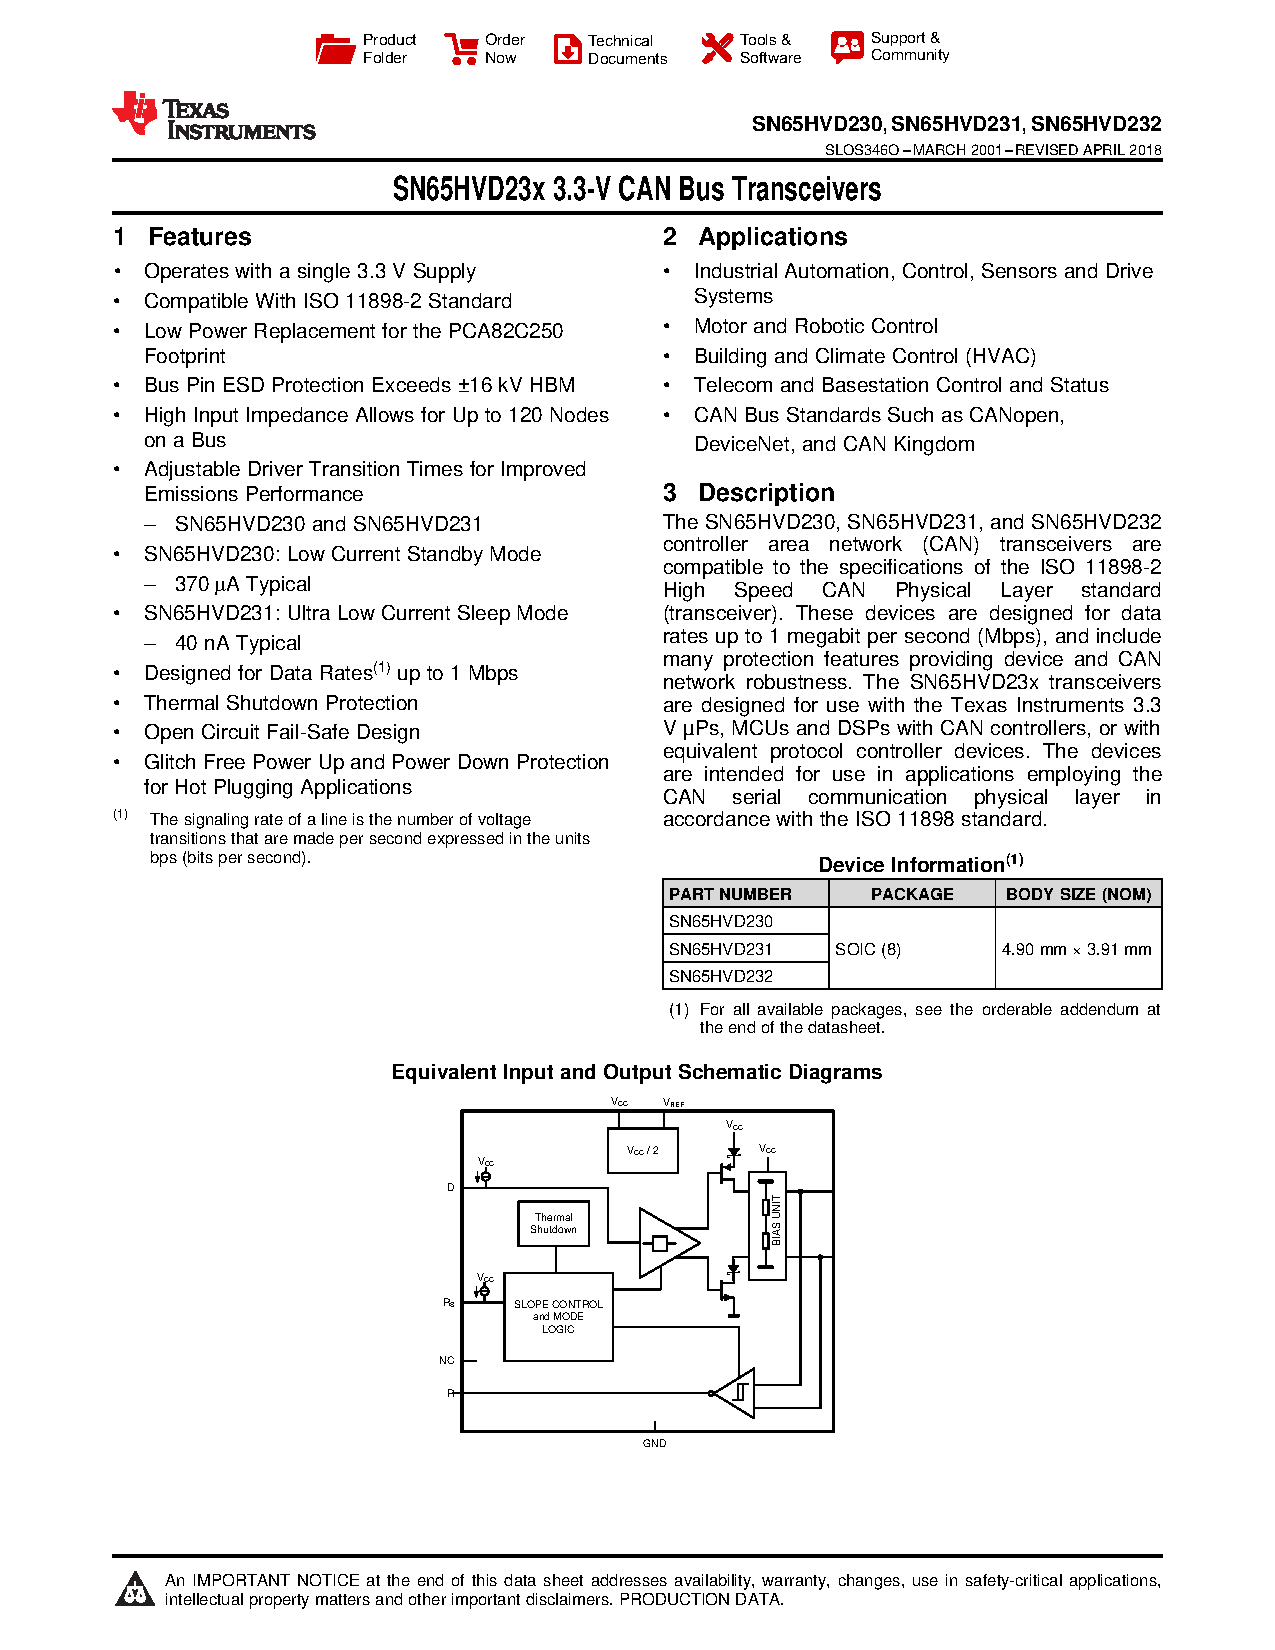
\includegraphics[page=1, width=0.95\textwidth]{DATASHEET/sn65hvd230.pdf}

	\vspace{4mm}
	\includegraphics[page=40, width=0.95\textwidth]{DATASHEET/sn65hvd230.pdf}
\end{center}

\newpage
\cleardoublepage % Limpia cualquier residuo de contadores anteriores
\refstepcounter{section}
\def\thesection{D} % <--- Fuerza a que el valor de la referencia sea solo "D"
\label{anexo:esp32}
\begin{center}
	\bfseries Apéndice D \\
	\normalfont\bfseries\itshape Hoja de Datos Técnicos del Módulo ESP32-S3-WROOM-1-N16R8
\end{center}
\addcontentsline{toc}{section}{Apéndice D: Hoja de Datos Técnicos del Módulo ESP32-S3-WROOM-1-N16R8}

\vspace{4mm}

Módulo Espressif ESP32-S3-WROOM-1-N16R8 (16~MB flash, 8~MB PSRAM octal), con controlador TWAI.

\begin{center}
	\includegraphics[page=2, width=0.91\textwidth]{DATASHEET/ESP32-S3.pdf}

	\vspace{4mm}
	\includegraphics[page=15, width=0.95\textwidth]{DATASHEET/ESP32-S3.pdf}

	
\end{center}

\newpage
\cleardoublepage % Limpia cualquier residuo de contadores anteriores
\refstepcounter{section}
\def\thesection{E} % <--- Fuerza a que el valor de la referencia sea solo "E"
\label{anexo:ssd1306}
\begin{center}
	\bfseries Apéndice E \\
	\normalfont\bfseries\itshape Hoja de Datos Técnicos del Controlador de Pantalla OLED SSD1306
\end{center}
\addcontentsline{toc}{section}{Apéndice E: Hoja de Datos Técnicos del Controlador de Pantalla OLED SSD1306}

\vspace{4mm}

Módulo de pantalla OLED I2C de 0,96", $128\times64$ píxeles, basado en el controlador SSD1306 \citep{ssd1306_datasheet}, con dirección I2C configurable entre \texttt{0x3C} y \texttt{0x3D}. Se reproducen las páginas de especificaciones básicas y el plano de dimensiones mecánicas del módulo.

\begin{center}
	\includegraphics[page=5, width=0.885\textwidth]{DATASHEET/OLED.pdf}

	\vspace{4mm}
	\includegraphics[page=6, width=0.95\textwidth]{DATASHEET/OLED.pdf}
\end{center}

\newpage
\cleardoublepage % Limpia cualquier residuo de contadores anteriores
\refstepcounter{section}
\def\thesection{F} % <--- Fuerza a que el valor de la referencia sea solo "F"
\label{anexo:fusible_ptc}
\begin{center}
	\bfseries Apéndice F \\
	\normalfont\bfseries\itshape Hoja de Datos Técnicos del Fusible PTC Reseteable, Serie BSMD1812
\end{center}
\addcontentsline{toc}{section}{Apéndice F: Hoja de Datos Técnicos del Fusible PTC Reseteable, Serie BSMD1812}

\vspace{4mm}

Fusible autorrecuperable PPTC de la serie BSMD1812 (encapsulado SMD 1812), con corriente de mantenimiento ($I_{hold}$) de 1{,}5~A y de disparo ($I_{trip}$) de 3{,}0~A \citep{bourns_bsmd1812}, primera línea de protección contra sobrecorriente en la línea de 12~V del conector OBD-II.

\begin{center}
	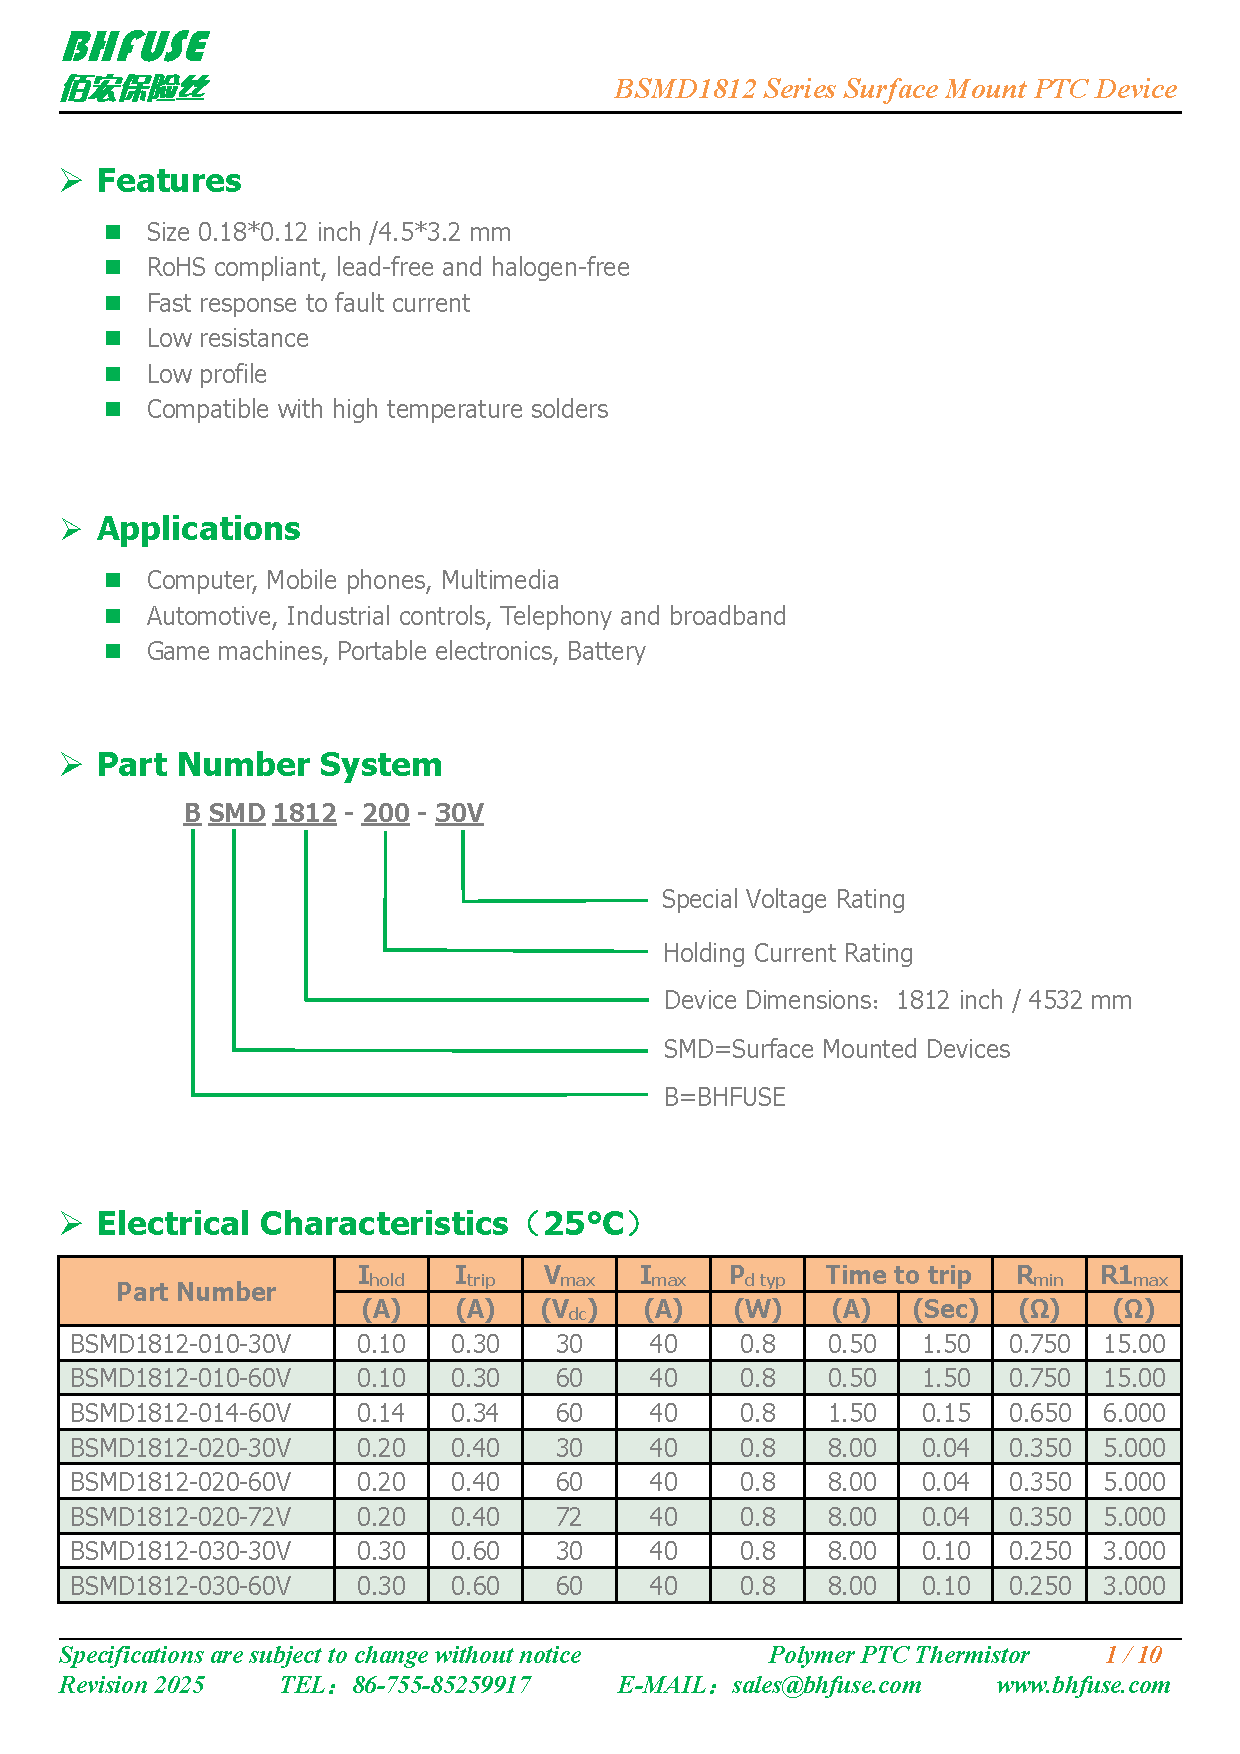
\includegraphics[page=1, width=0.85\textwidth]{DATASHEET/FUSE.pdf}
\end{center}

\newpage
\cleardoublepage
\refstepcounter{section}
\def\thesection{G}
\label{anexo:ss36}
\begin{center}
	\bfseries Apéndice G \\
	\normalfont\bfseries\itshape Diodo Schottky SS34 — Especificaciones Técnicas
\end{center}
\addcontentsline{toc}{section}{Apéndice G: Diodo Schottky SS34}

\vspace{4mm}

Diodo Schottky SS34 (familia SS32 a SS3200, MDD/China Base Electronics), encapsulado DO-214AC (SMA), con tensión inversa repetitiva máxima ($V_{RRM}$) de 40~V y corriente media rectificada ($I_O$) de 3~A \citep{onsemi_ss36}, usado como protección de polaridad inversa en la línea de 12~V del OBD-II. La fila correspondiente a SS34 es la aplicable a este proyecto.

\begin{center}
	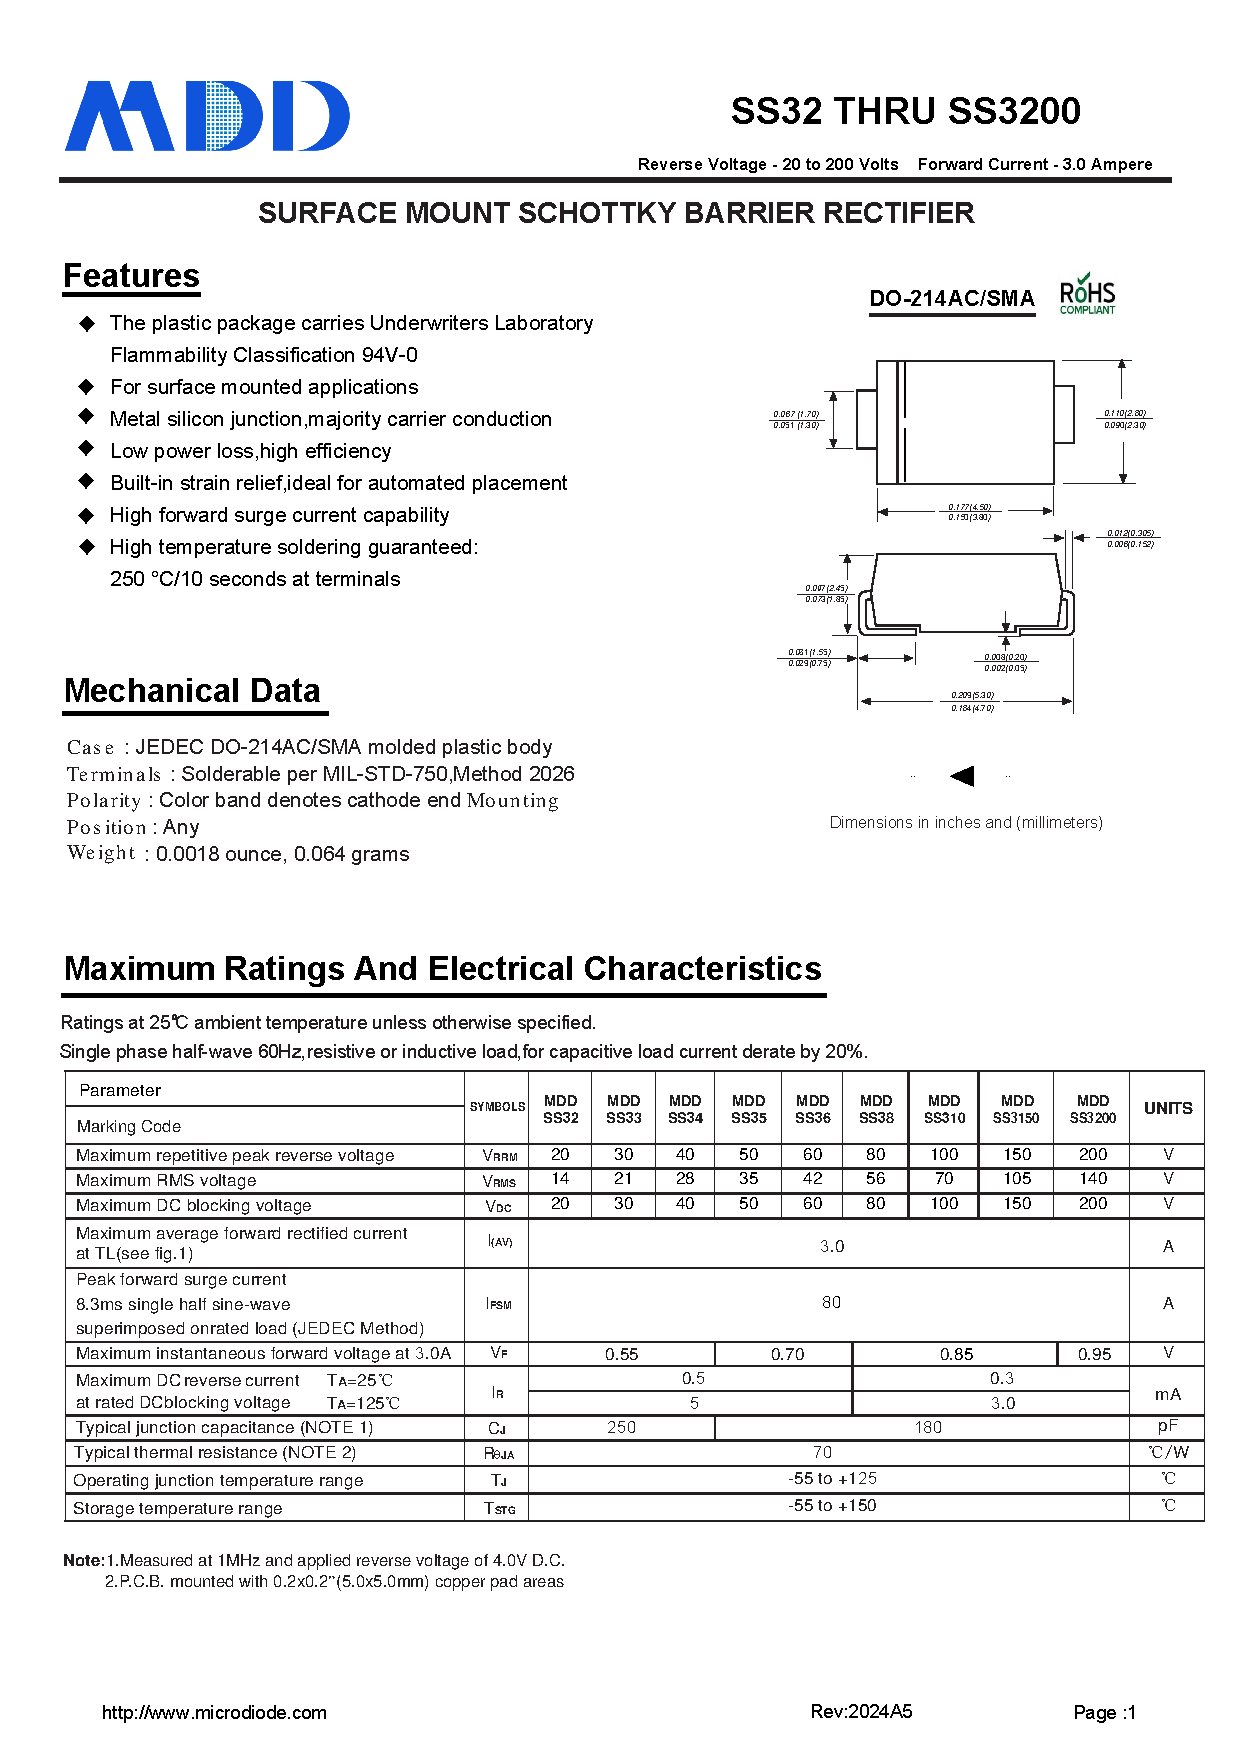
\includegraphics[page=1, width=0.85\textwidth]{DATASHEET/DIODE SS34.pdf}
\end{center}

\newpage
\cleardoublepage
\refstepcounter{section}
\def\thesection{H}
\label{apendiceG}
\begin{center}
	\bfseries Apéndice H \\
	\normalfont\bfseries\itshape Hoja de Datos Técnicos del Diodo Supresor de Tensión Transitoria (TVS) SMAJ18A
\end{center}
\addcontentsline{toc}{section}{Apéndice H: Hoja de Datos Técnicos del Diodo Supresor de Tensión Transitoria (TVS) SMAJ18A}

\vspace{4mm}

Diodo TVS Littelfuse serie SMAJ, modelo SMAJ18A (DO-214AC/SMA, 400~W pico), con tensión de trabajo (\textit{stand-off}) de 18~V y tensión de sujeción máxima de 29{,}2~V a 13{,}7~A \citep{vishay_smaj28a}, usado como protección contra transitorios de \textit{load dump} y ESD en la línea de 12~V.

\begin{center}
	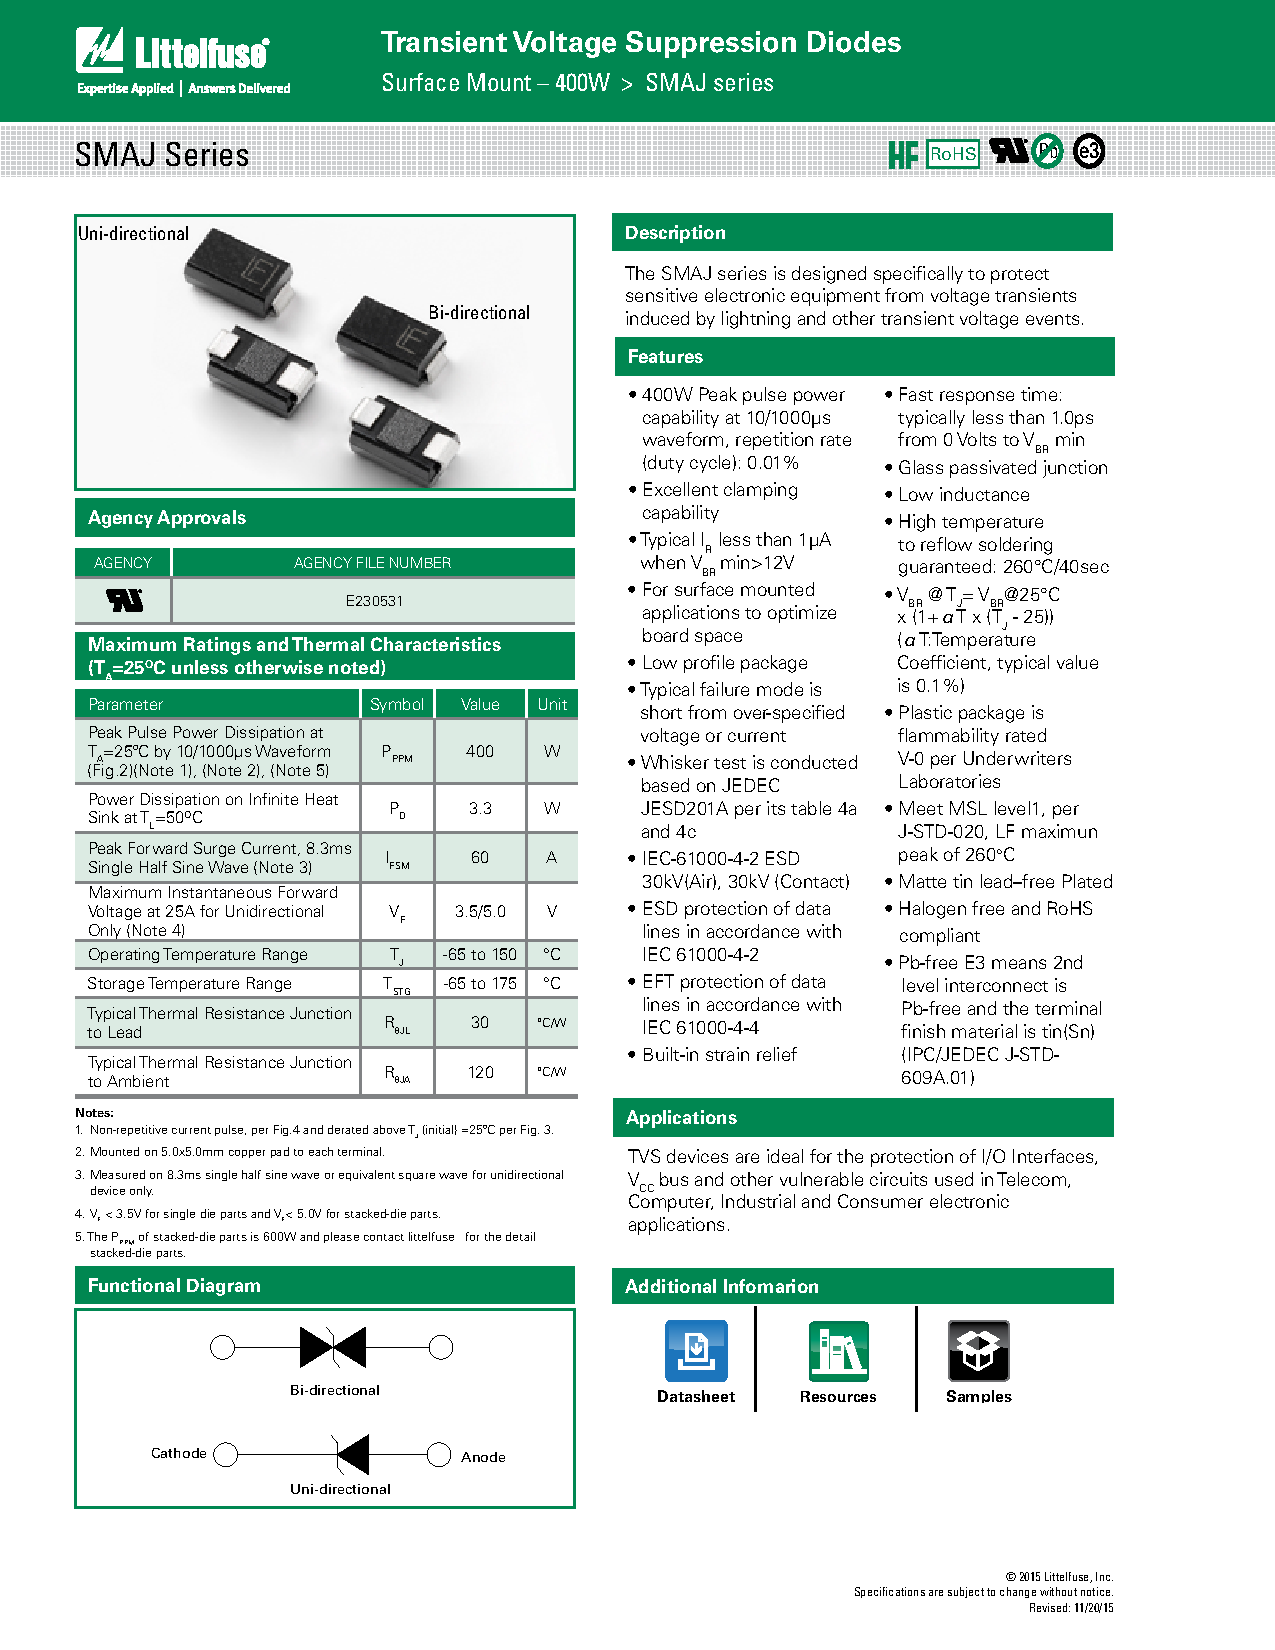
\includegraphics[page=1, width=0.85\textwidth]{DATASHEET/SMAJ18A.pdf}
\end{center}

\newpage
\cleardoublepage
\refstepcounter{section}
\def\thesection{I}
\label{anexo:tps54302}
\begin{center}
	\bfseries Apéndice I \\
	\normalfont\bfseries\itshape Hoja de Datos Técnicos del Convertidor Buck Síncrono TPS54302DDCR
\end{center}
\addcontentsline{toc}{section}{Apéndice I: Hoja de Datos Técnicos del Convertidor Buck Síncrono TPS54302DDCR}

\vspace{4mm}

Convertidor \textit{buck} síncrono TPS54302DDCR (Texas Instruments), primera etapa de la cadena de regulación de dos rieles (Capítulo~3): 12~V~$\rightarrow$~5~V, entrada de 4{,}5~V a 28~V, hasta 3~A continuos a 400~kHz, encapsulado SOT-23-6. Se reproducen las páginas de características y de dimensiones del encapsulado.

\begin{center}
	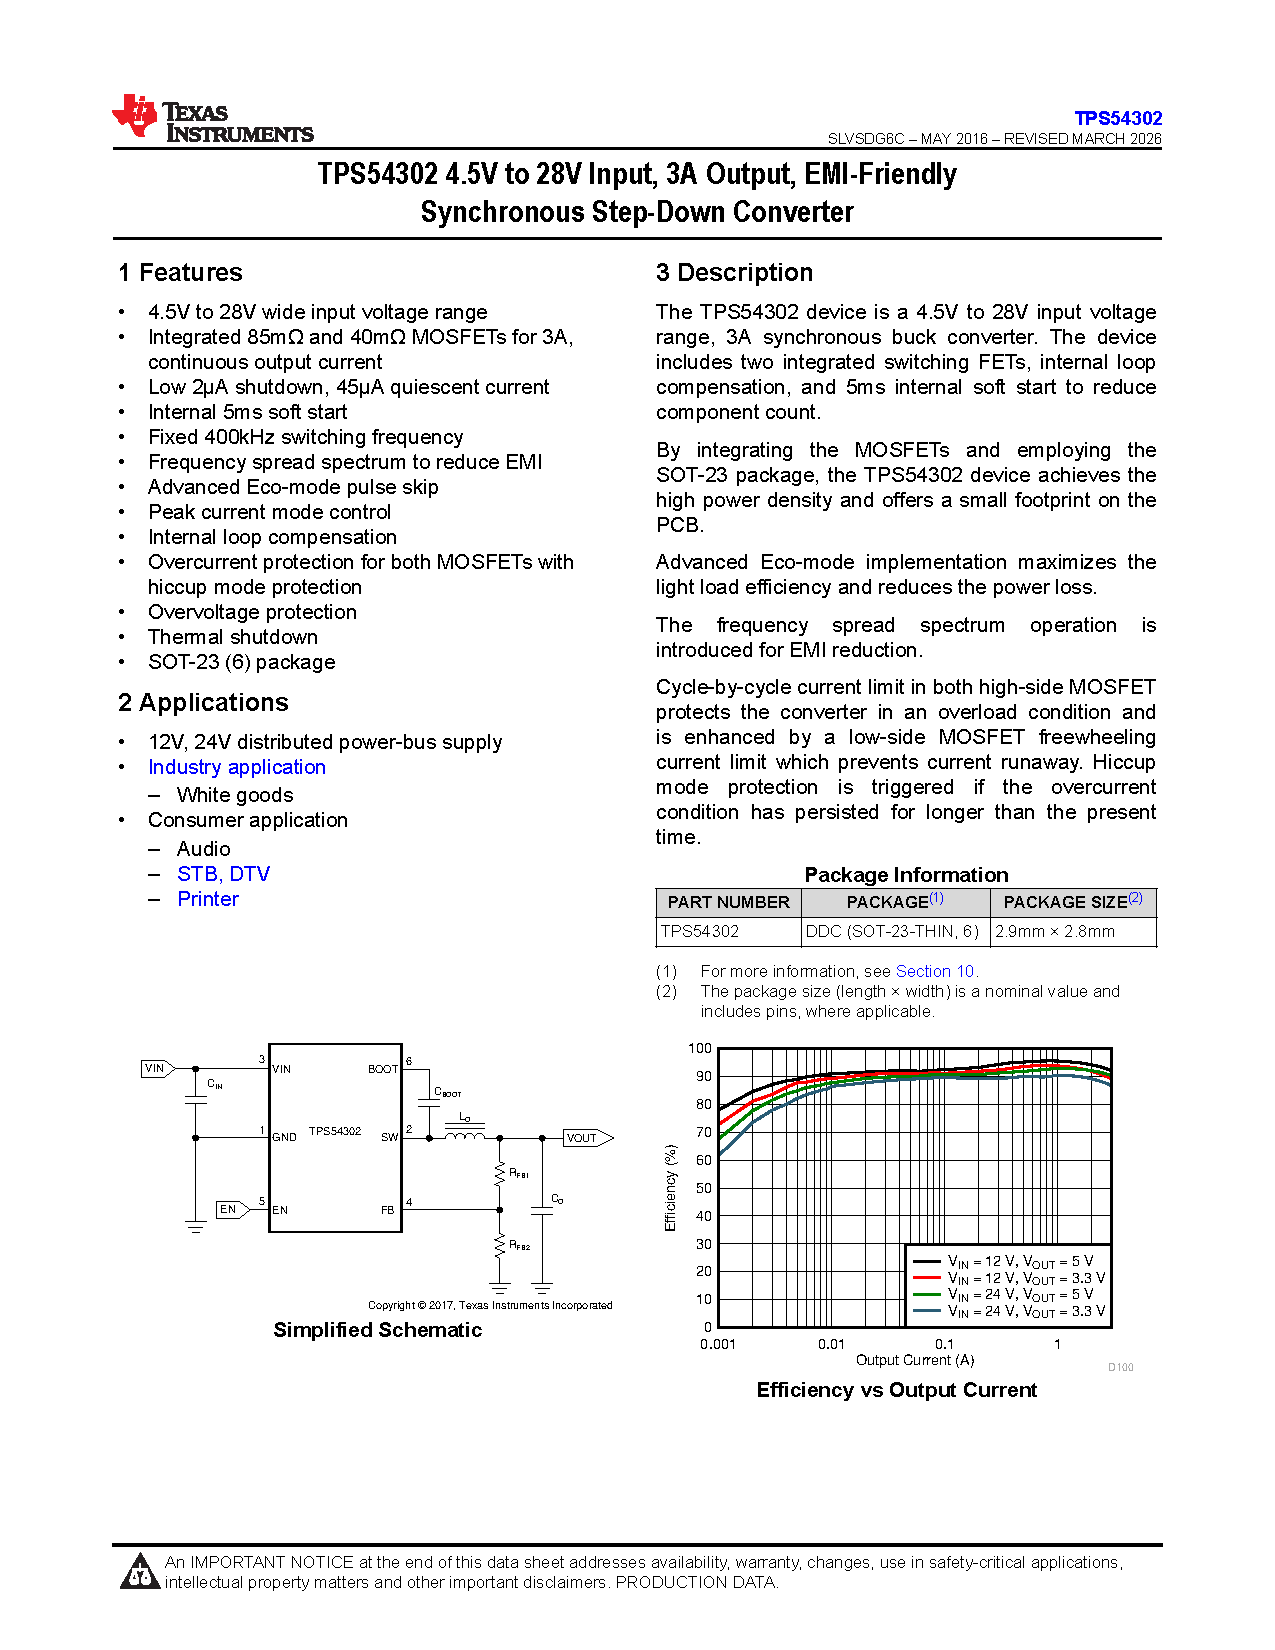
\includegraphics[page=1, width=0.85\textwidth]{DATASHEET/TPS54302.pdf}

	\vspace{4mm}
	\includegraphics[page=14, width=0.98\textwidth]{DATASHEET/TPS54302.pdf}
\end{center}

\newpage
\cleardoublepage
\refstepcounter{section}
\def\thesection{J}
\label{anexo:ams1117}
\begin{center}
	\bfseries Apéndice J \\
	\normalfont\bfseries\itshape Hoja de Datos Técnicos del Regulador Lineal AMS1117-3.3
\end{center}
\addcontentsline{toc}{section}{Apéndice J: Hoja de Datos Técnicos del Regulador Lineal AMS1117-3.3}

\vspace{4mm}

LDO AMS1117-3.3, alimenta el riel~1 permanentemente activo (ESP32-S3-WROOM-1-N16R8 y SN65HVD230) a partir de los 5~V del TPS54302DDCR (Apéndice~I), con capacidad de hasta 1~A continuo.

\begin{center}
	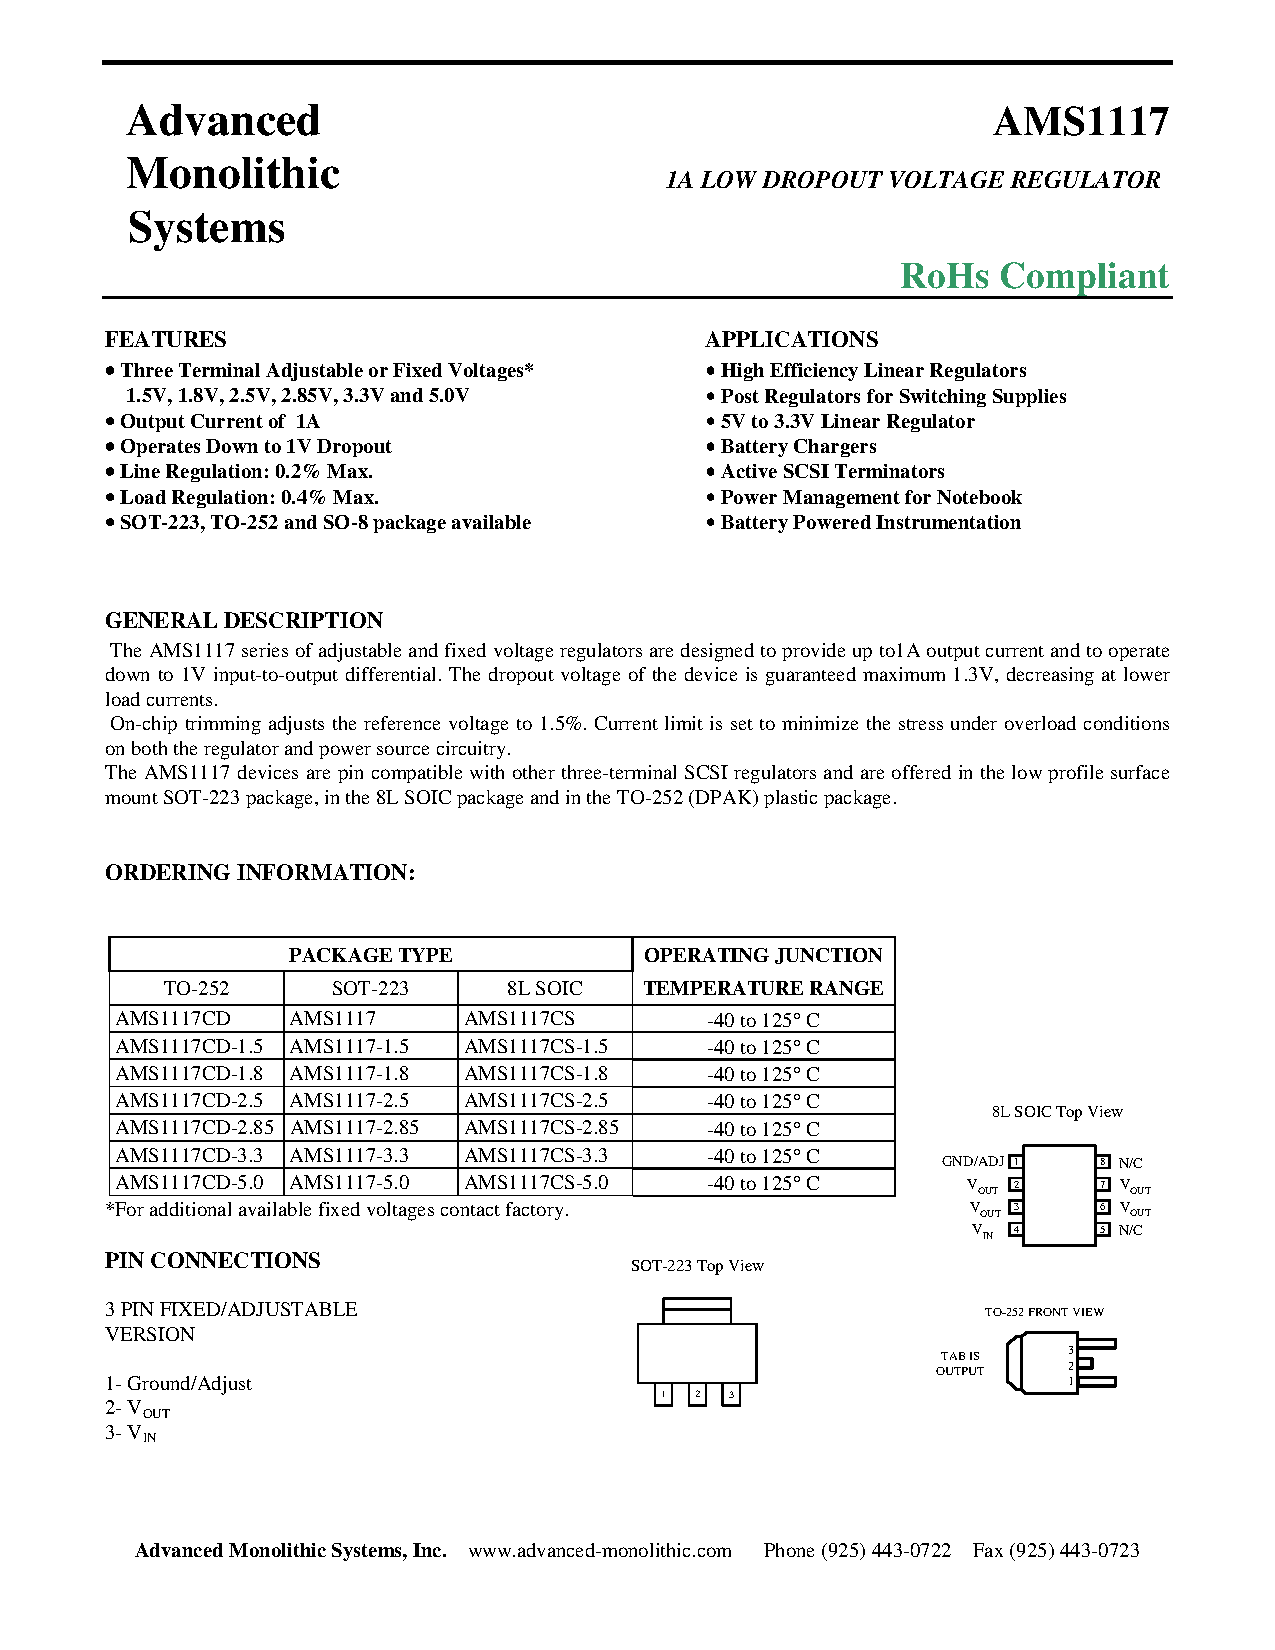
\includegraphics[page=1, width=0.95\textwidth]{DATASHEET/AMS1117.pdf}
\end{center}

\newpage
\cleardoublepage
\refstepcounter{section}
\def\thesection{K}
\label{anexo:ap2112k}
\begin{center}
	\bfseries Apéndice K \\
	\normalfont\bfseries\itshape Hoja de Datos Técnicos del Regulador Lineal AP2112K-3.3TRG1
\end{center}
\addcontentsline{toc}{section}{Apéndice K: Hoja de Datos Técnicos del Regulador Lineal AP2112K-3.3TRG1}

\vspace{4mm}

LDO AP2112K-3.3TRG1 (Diodes Incorporated), alimenta el riel~2 conmutado (OLED, microSD) vía el interruptor de carga TPS22918 (Apéndice~L), con capacidad de hasta 600~mA y bajo nivel de ruido.

\begin{center}
	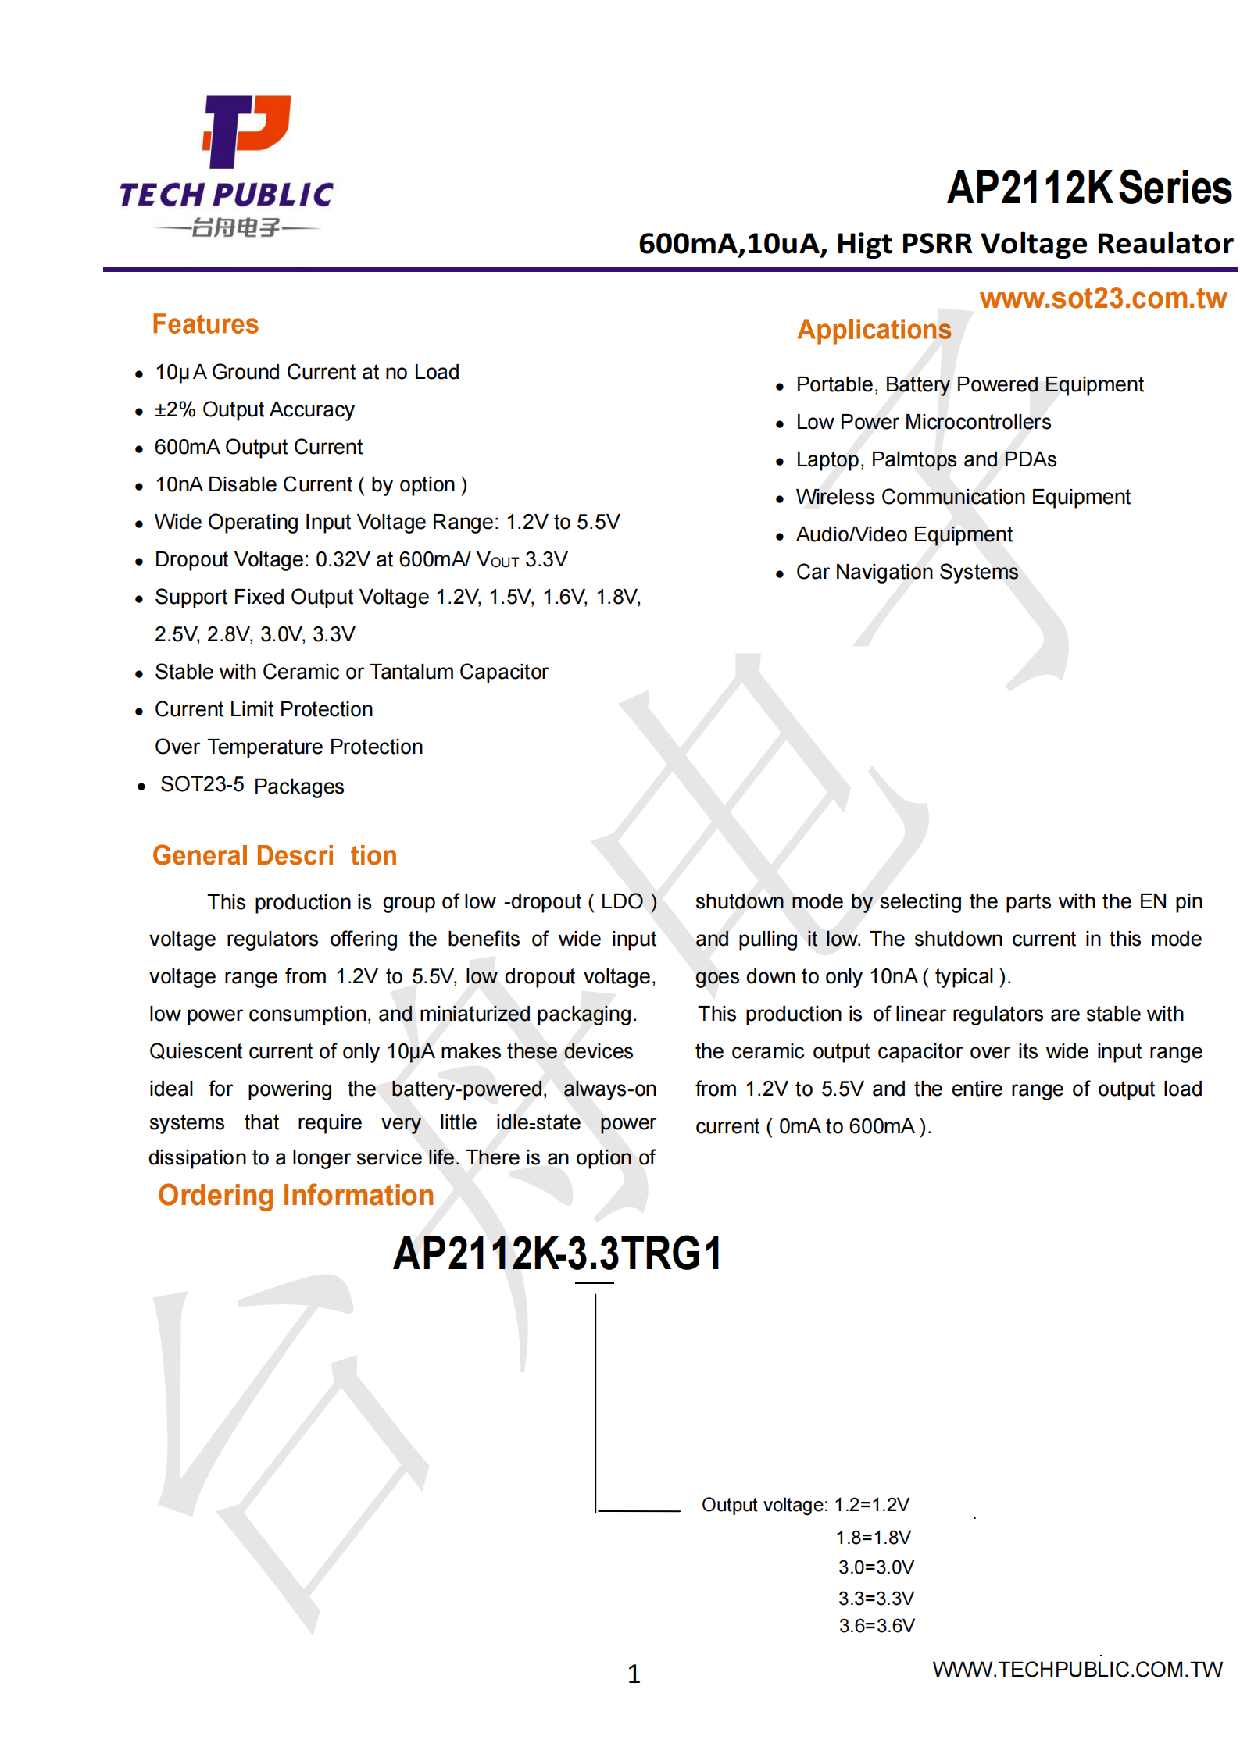
\includegraphics[page=1, width=0.85\textwidth]{DATASHEET/AP2112K.pdf}
\end{center}

\newpage
\cleardoublepage
\refstepcounter{section}
\def\thesection{L}
\label{anexo:tps22918}
\begin{center}
	\bfseries Apéndice L \\
	\normalfont\bfseries\itshape Hoja de Datos Técnicos del Interruptor de Carga TPS22918
\end{center}
\addcontentsline{toc}{section}{Apéndice L: Hoja de Datos Técnicos del Interruptor de Carga TPS22918}

\vspace{4mm}

Interruptor de carga (\textit{load switch}) TPS22918 (Texas Instruments), conecta/desconecta el riel~2 de 3{,}3~V (OLED, microSD) bajo control de un GPIO del ESP32-S3, implementando el modo de bajo consumo del Capítulo~3. $R_{ON}\approx 52\,\text{m}\Omega$, control configurable del tiempo de subida.

\begin{center}
	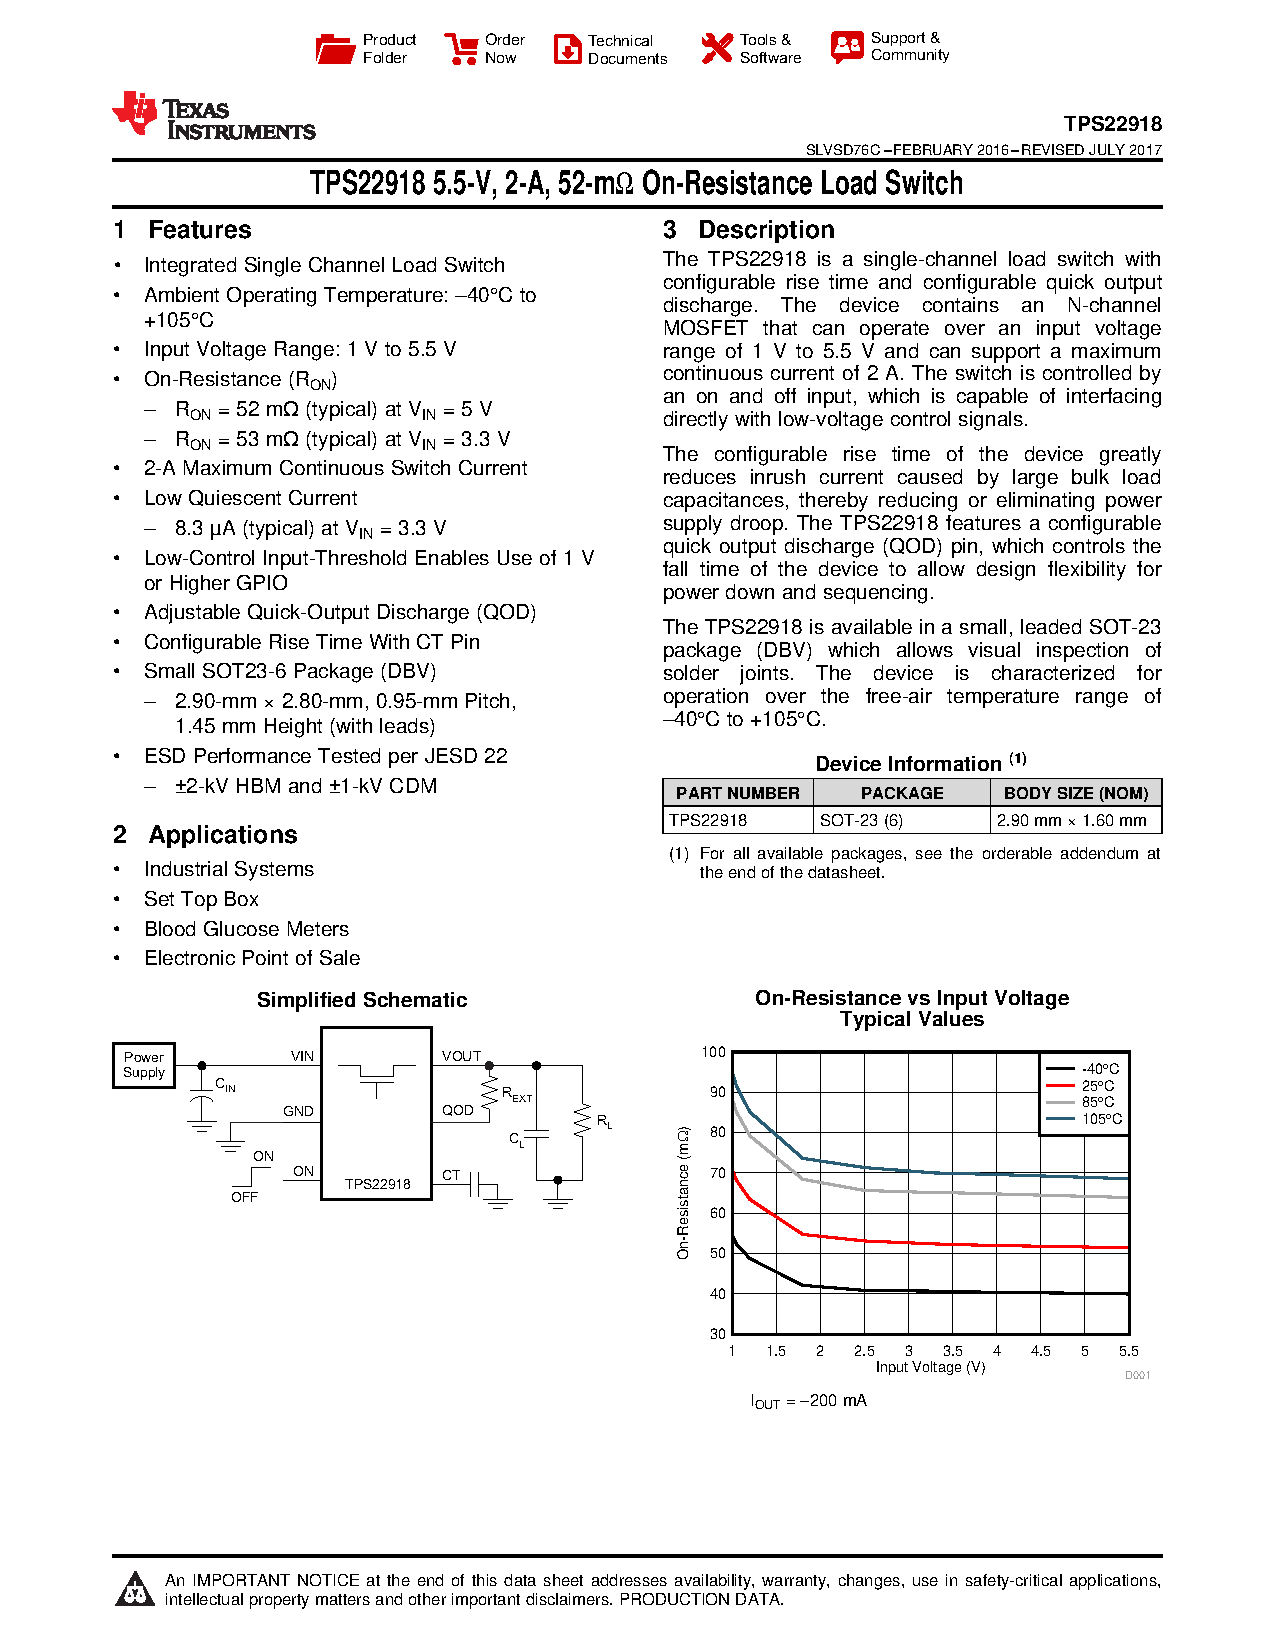
\includegraphics[page=1, width=0.95\textwidth]{DATASHEET/TPS22918.pdf}

	\vspace{4mm}
	\includegraphics[page=16, width=1\textwidth]{DATASHEET/TPS22918.pdf}

	\vspace{4mm}
	\includegraphics[page=18, width=1\textwidth]{DATASHEET/TPS22918.pdf}
\end{center}

\newpage
\cleardoublepage
\refstepcounter{section}
\def\thesection{M}
\label{anexo:esquematico_pcb}
\begin{center}
	\bfseries Apéndice M \\
	\normalfont\bfseries\itshape Esquemático Eléctrico Completo y Diseño de la PCB
\end{center}
\addcontentsline{toc}{section}{Apéndice M: Esquemático Eléctrico Completo y Diseño de la PCB}

\vspace{4mm}

Esquemático eléctrico completo del sistema (diseñado en Altium Designer), disposición física de la PCB (vista de capas y ruteado) y reporte de la pila de capas (\textit{board stack}), referenciados desde la Sección de diseño de hardware del Capítulo~3.

\begin{center}
	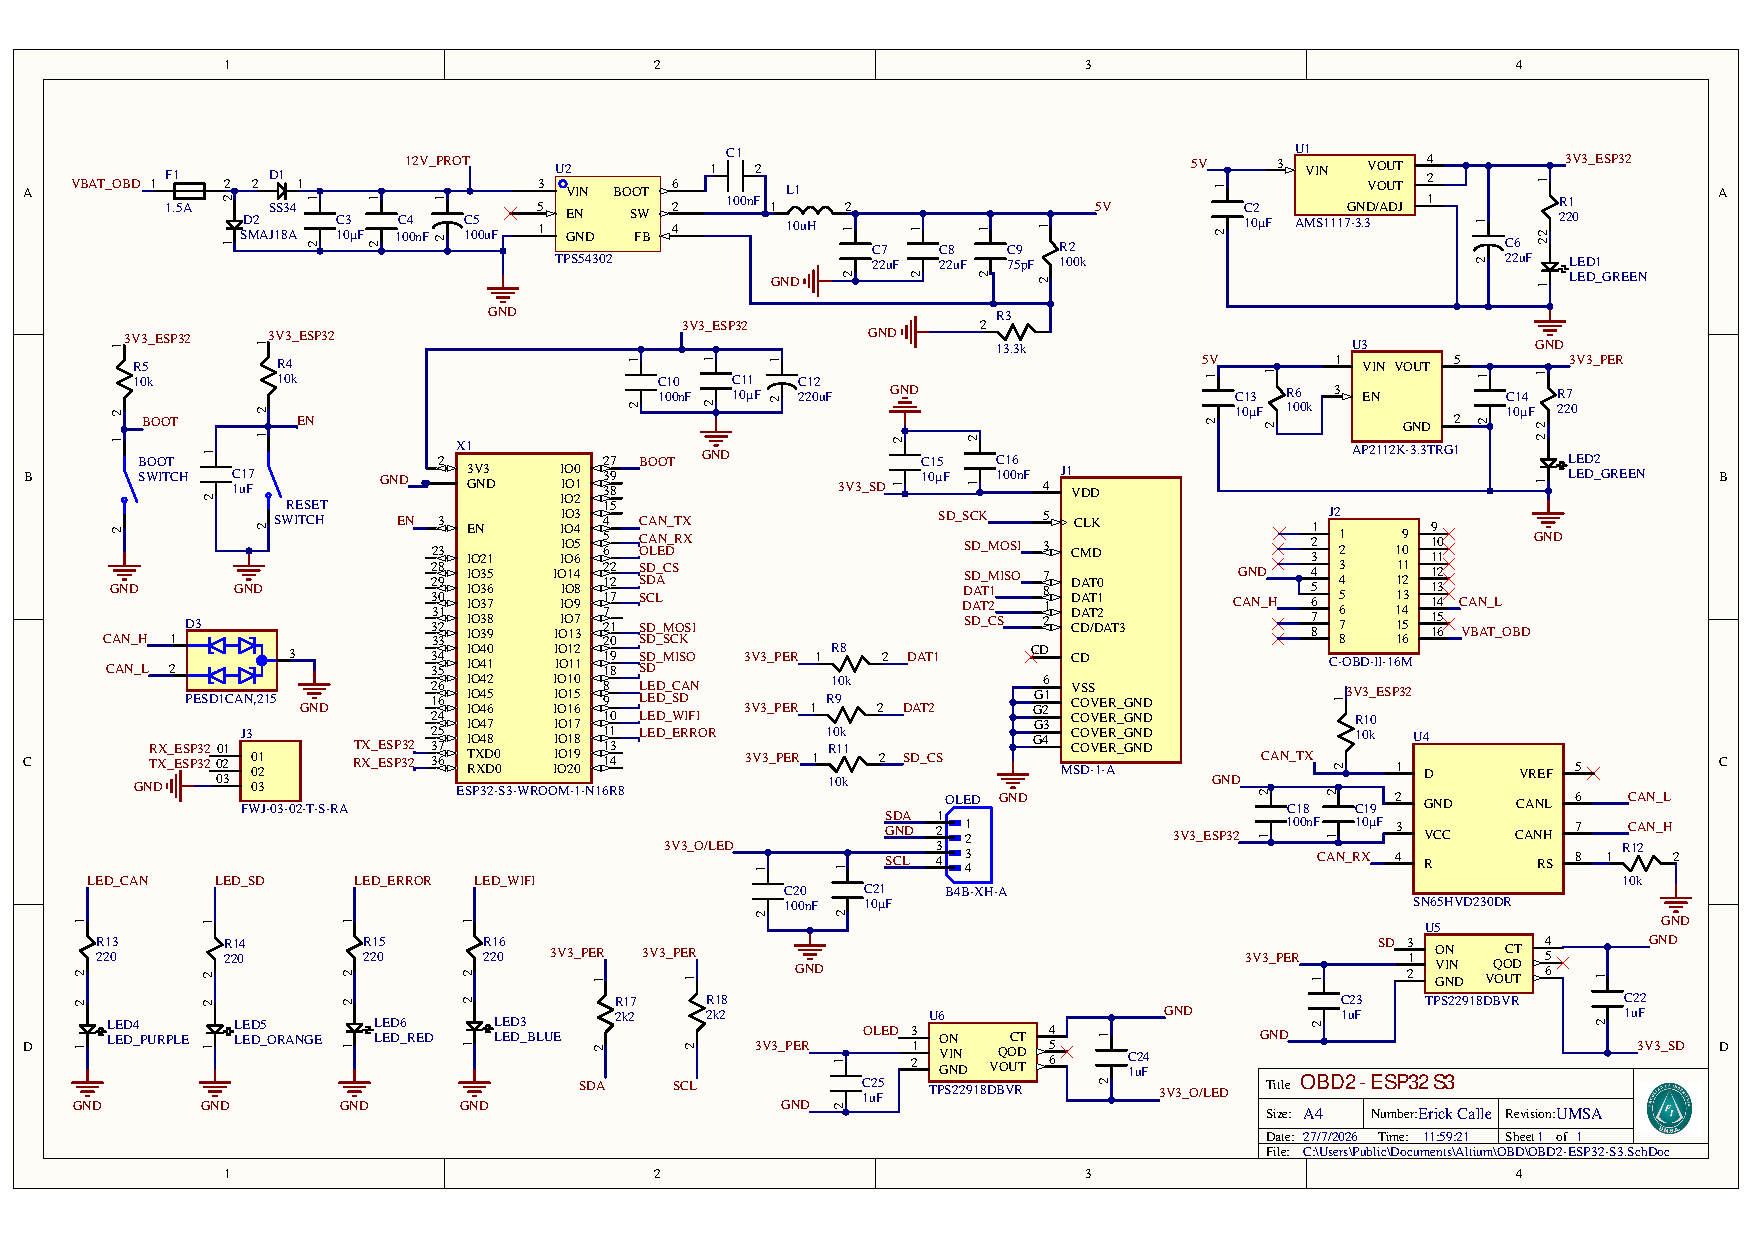
\includegraphics[page=1, width=\textwidth]{DATASHEET/OBD2.pdf}

	\vspace{4mm}
	\includegraphics[page=2, width=0.7\textwidth]{DATASHEET/OBD2.pdf}

\end{center}

\newpage
\cleardoublepage
\refstepcounter{section}
\def\thesection{N}
\label{anexo:bom_detalle}
\begin{center}
	\bfseries Apéndice N \\
	\normalfont\bfseries\itshape Lista de Materiales (BOM) — Detalle de Fabricación
\end{center}
\addcontentsline{toc}{section}{Apéndice N: Lista de Materiales (BOM) — Detalle de Fabricación}

\vspace{4mm}

A diferencia de la Tabla~\ref{bom} del Capítulo~3 —que agrupa los componentes por bloque funcional con fines explicativos—, este apéndice reproduce la lista de materiales tal como se exportó para la fabricación y el ensamblaje de la PCB.
\begin{center}
	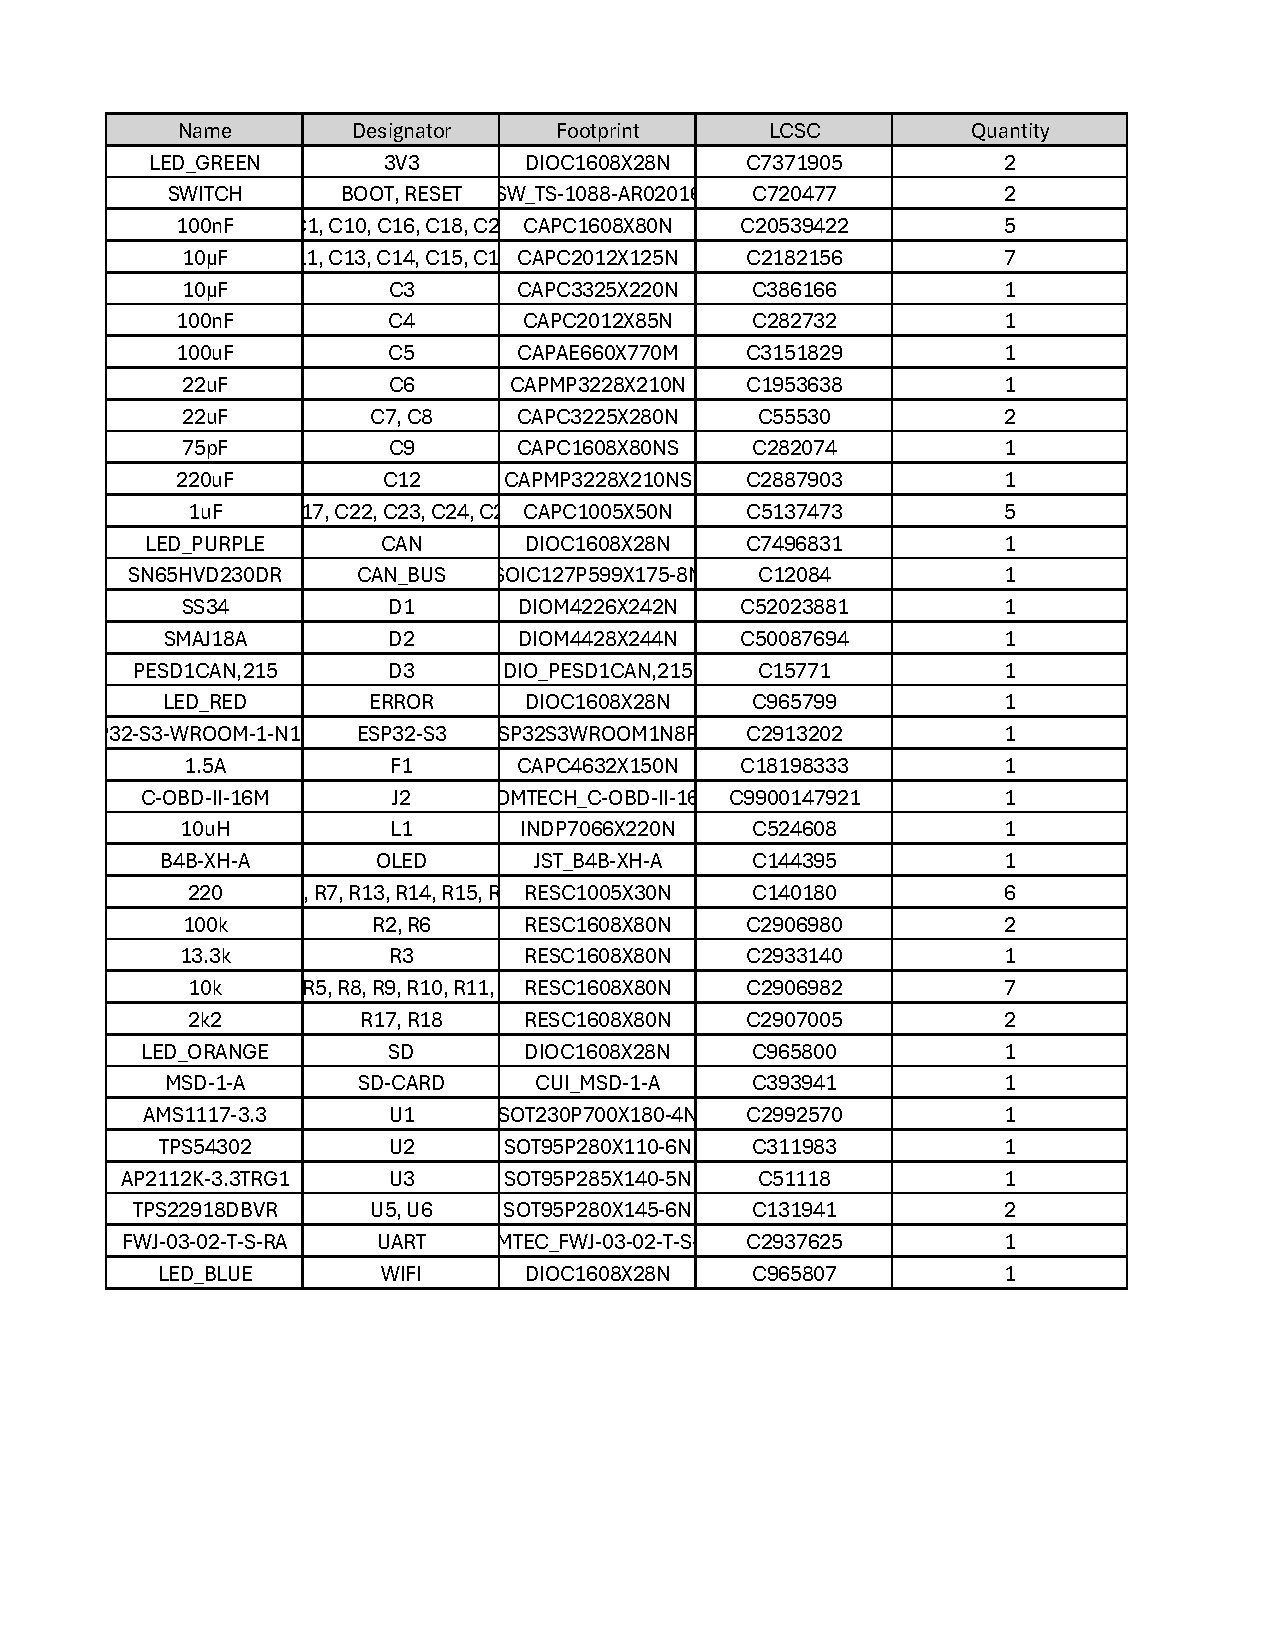
\includegraphics[page=1, width=0.92\textwidth]{DATASHEET/BOOM.pdf}
\end{center}

\newpage
\cleardoublepage
\refstepcounter{section}
\def\thesection{O}
\label{anexo:pids_vehiculos}
\begin{center}
	\bfseries Apéndice O \\
	\normalfont\bfseries\itshape PIDs OBD-II Soportados por los Vehículos de Prueba: Changan Honor y Nissan Vanette
\end{center}
\addcontentsline{toc}{section}{Apéndice O: PIDs OBD-II Soportados por los Vehículos de Prueba}

\vspace{4mm}

Listado completo y decodificado de los PIDs OBD-II (Modo~01) soportados por cada vehículo de validación, obtenido mediante el escaneo activo del Capítulo~3. Changan Honor: 34 PIDs, sin el PID~0x10 (MAF). Nissan Vanette: 33 PIDs, incluyendo el PID~0x10.

\begin{center}
	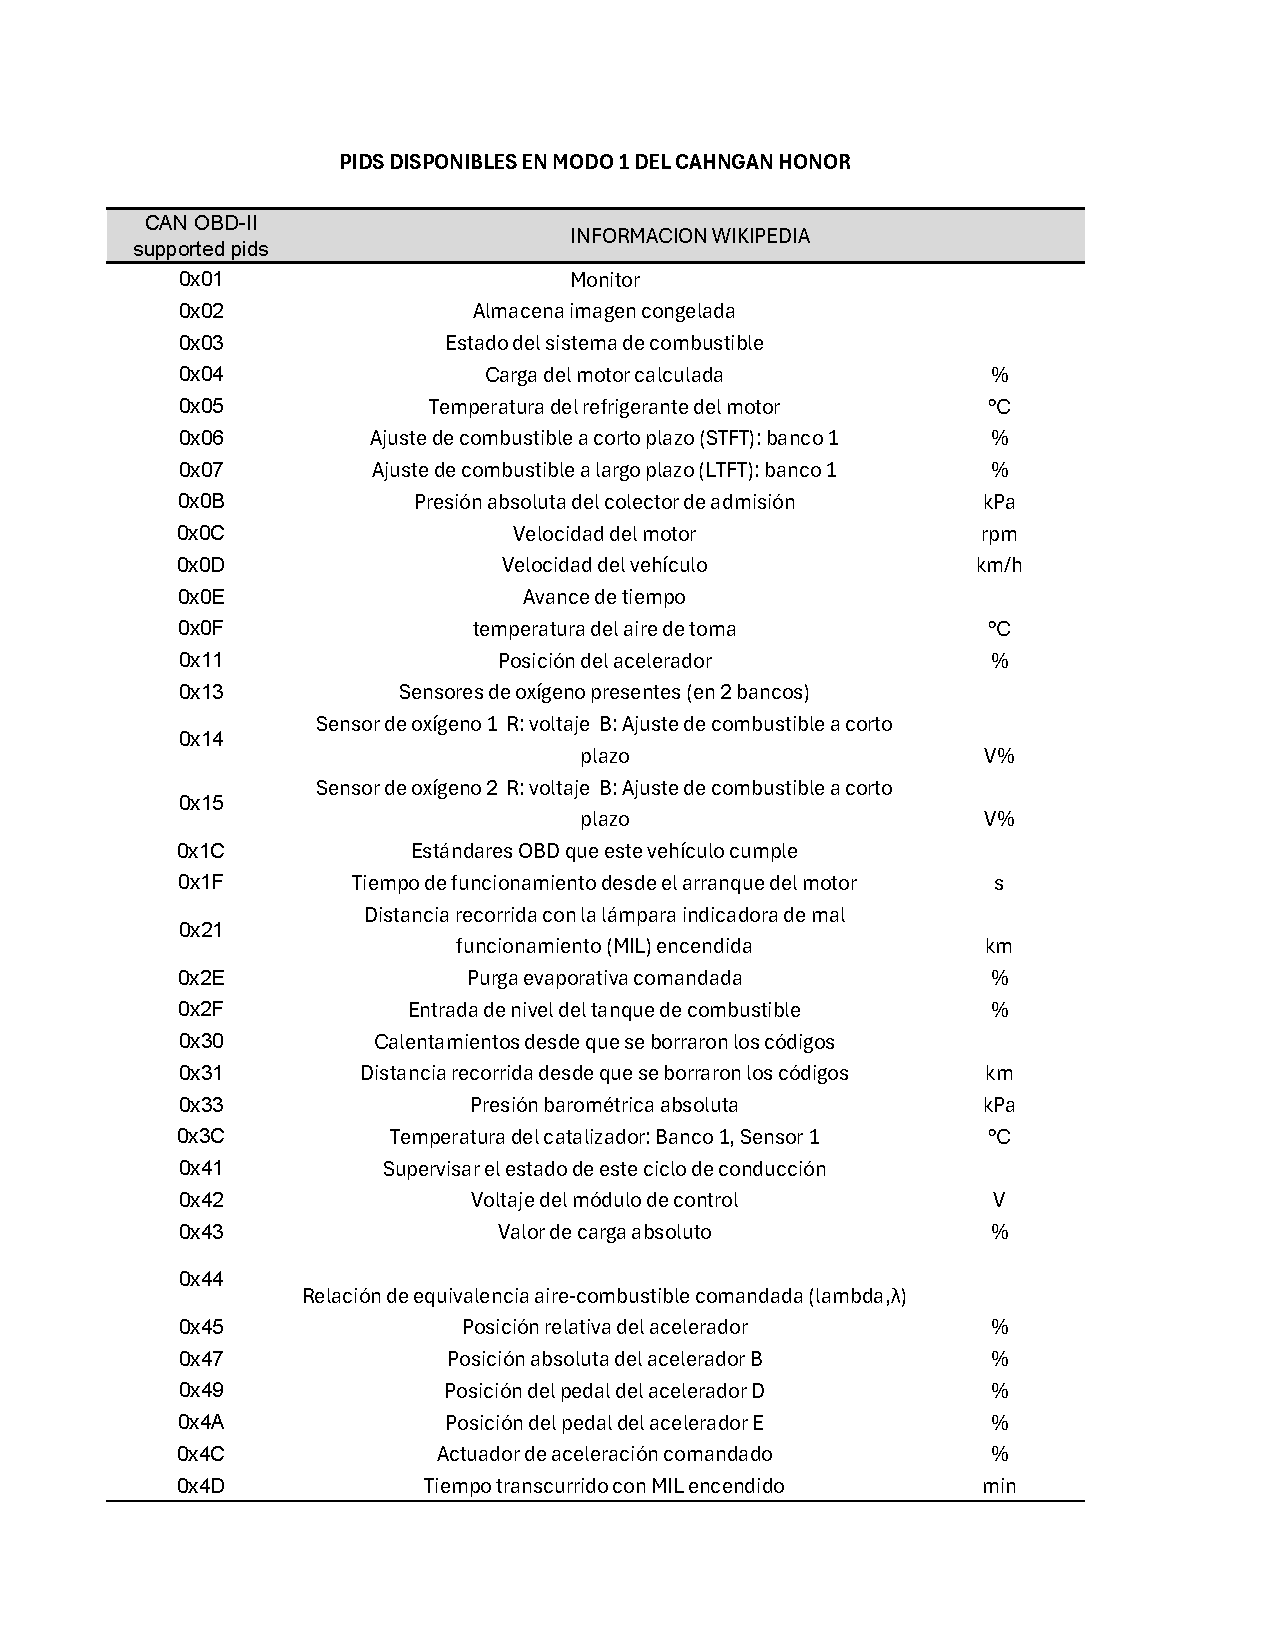
\includegraphics[page=1, width=0.94\textwidth]{DATASHEET/CHANGAN.pdf}

	\vspace{4mm}
	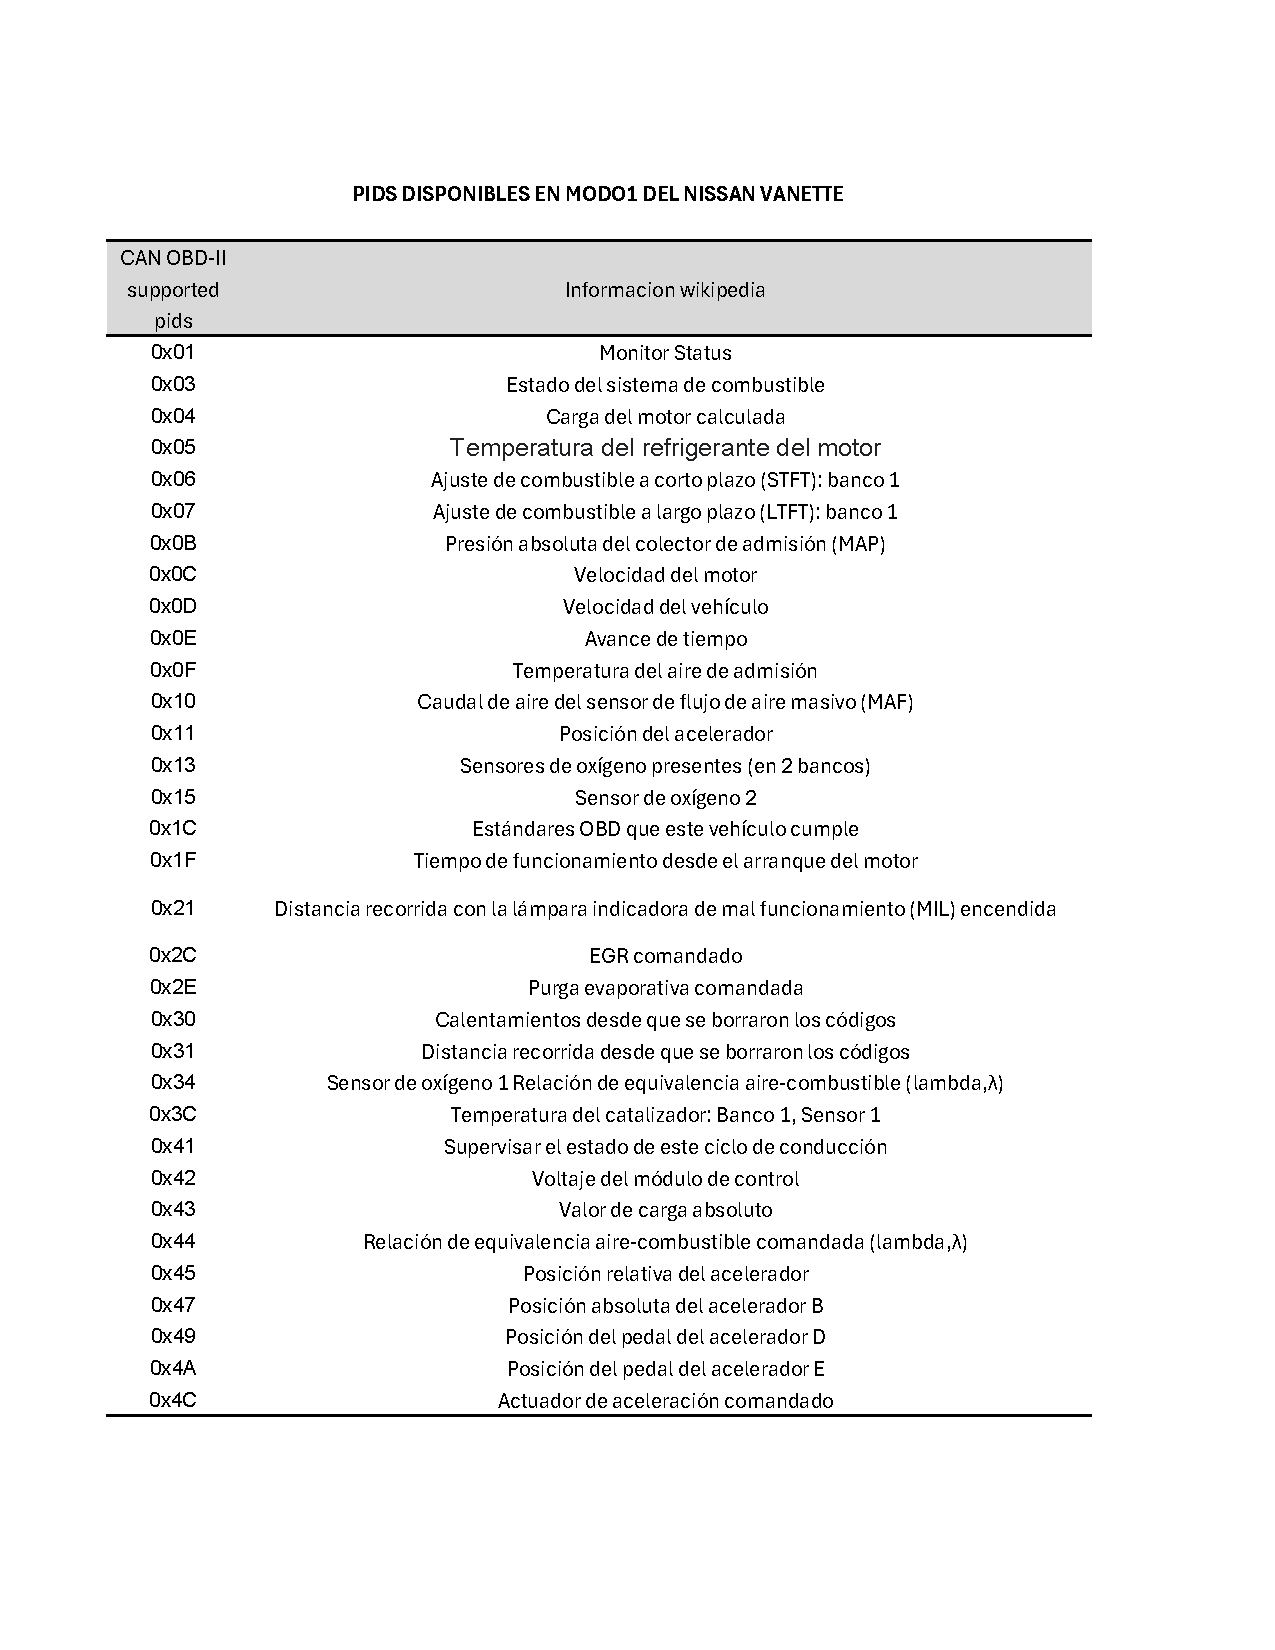
\includegraphics[page=1, width=1.1\textwidth]{DATASHEET/NISSAN.pdf}
\end{center}

\newpage
\cleardoublepage
\refstepcounter{section}
\def\thesection{P}
\label{anexo:mcp2515}
\begin{center}
	\bfseries Apéndice P \\
	\normalfont\bfseries\itshape Hoja de Datos Técnicos del Controlador CAN MCP2515 (Arquitectura Descartada)
\end{center}
\addcontentsline{toc}{section}{Apéndice P: Hoja de Datos Técnicos del Controlador CAN MCP2515 (Arquitectura Descartada)}

\vspace{4mm}

Controlador CAN independiente con interfaz SPI (Microchip), evaluado en la etapa inicial del proyecto y descartado en favor del periférico TWAI integrado en el ESP32-S3-WROOM-1-N16R8 (Apéndice~D). Se documenta únicamente como referencia del proceso de decisión de diseño, no como componente del sistema final.

\begin{center}
	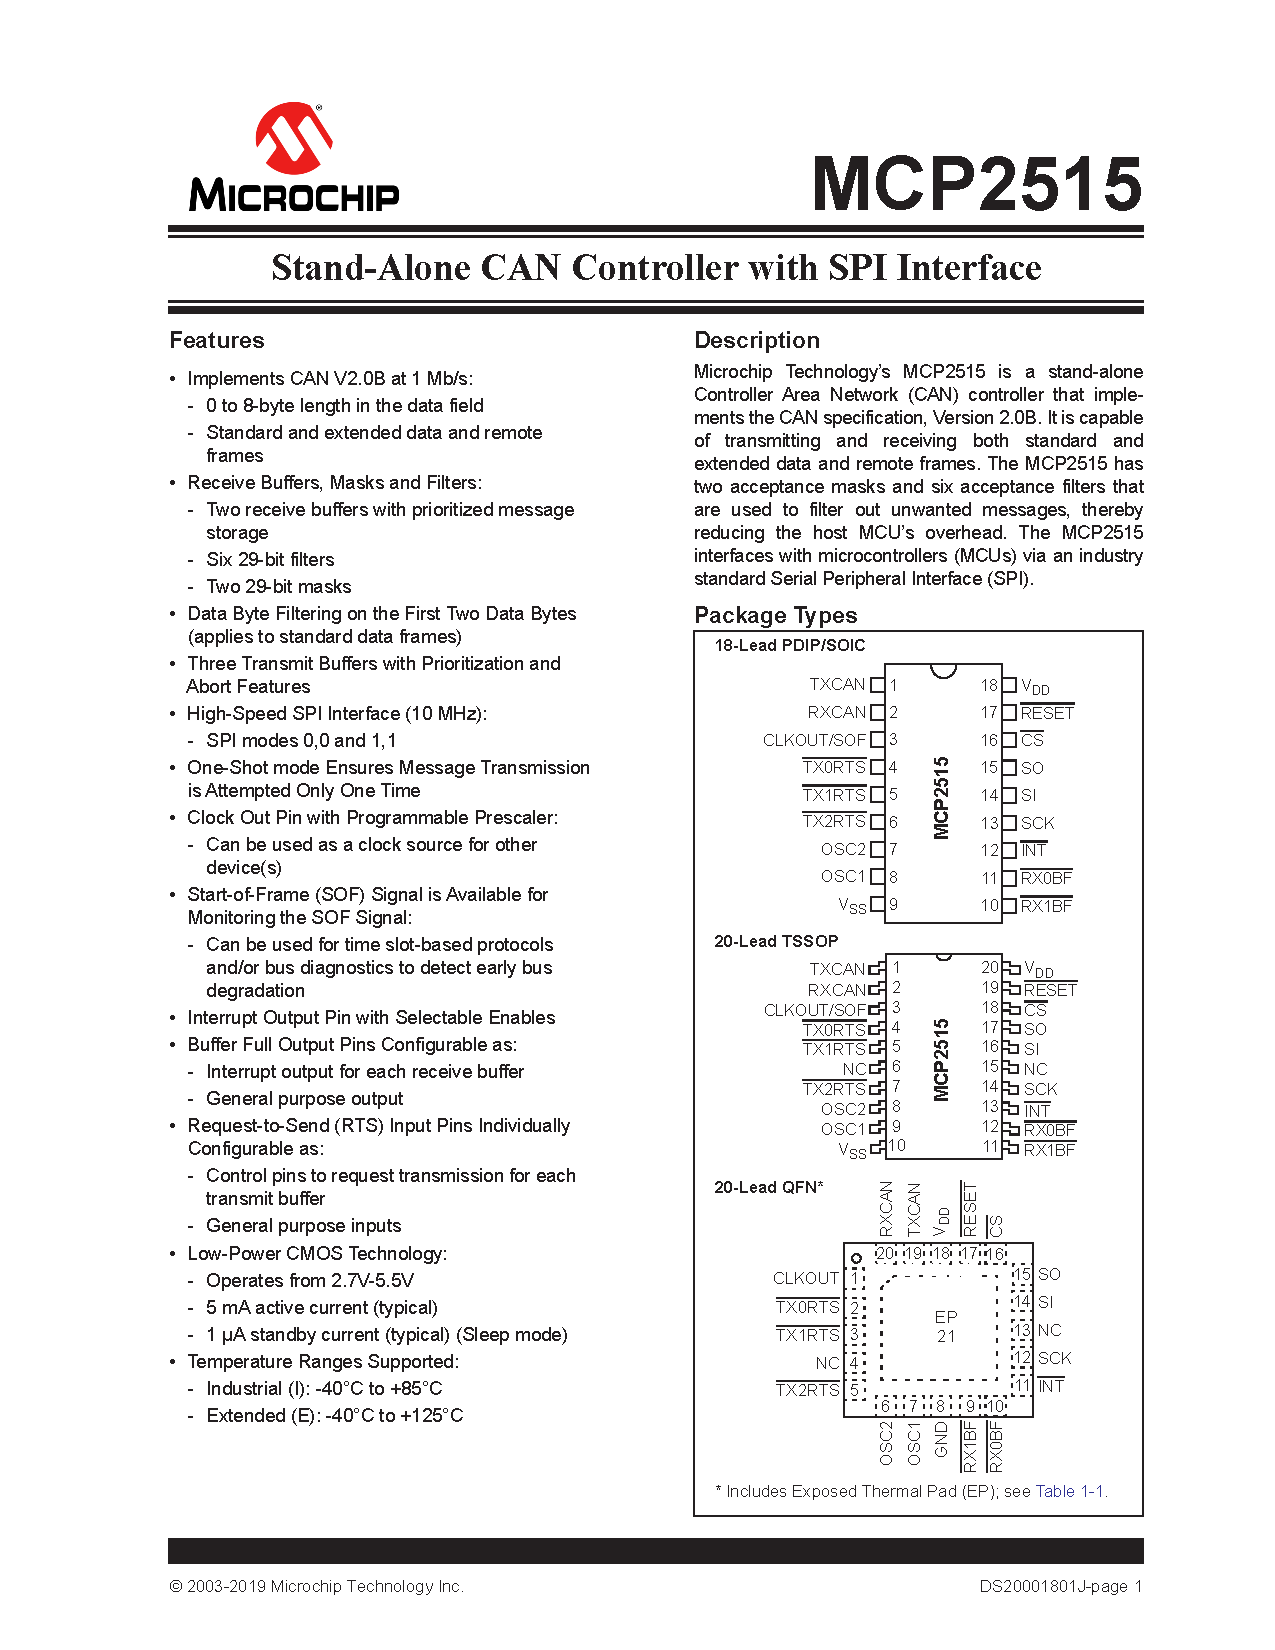
\includegraphics[page=1, width=0.89\textwidth]{DATASHEET/MCP2515.pdf}

	
\end{center}
	
\end{document}
